\documentclass[twoside]{book}

% Packages required by doxygen
\usepackage{calc}
\usepackage{doxygen}
\usepackage{graphicx}
\usepackage[utf8]{inputenc}
\usepackage{makeidx}
\usepackage{multicol}
\usepackage{multirow}
\usepackage{textcomp}
\usepackage[table]{xcolor}

% Font selection
\usepackage[T1]{fontenc}
\usepackage{mathptmx}
\usepackage[scaled=.90]{helvet}
\usepackage{courier}
\usepackage{amssymb}
\usepackage{sectsty}
\renewcommand{\familydefault}{\sfdefault}
\allsectionsfont{%
  \fontseries{bc}\selectfont%
  \color{darkgray}%
}
\renewcommand{\DoxyLabelFont}{%
  \fontseries{bc}\selectfont%
  \color{darkgray}%
}

% Page & text layout
\usepackage{geometry}
\geometry{%
  a4paper,%
  top=2.5cm,%
  bottom=2.5cm,%
  left=2.5cm,%
  right=2.5cm%
}
\tolerance=750
\hfuzz=15pt
\hbadness=750
\setlength{\emergencystretch}{15pt}
\setlength{\parindent}{0cm}
\setlength{\parskip}{0.2cm}
\makeatletter
\renewcommand{\paragraph}{%
  \@startsection{paragraph}{4}{0ex}{-1.0ex}{1.0ex}{%
    \normalfont\normalsize\bfseries\SS@parafont%
  }%
}
\renewcommand{\subparagraph}{%
  \@startsection{subparagraph}{5}{0ex}{-1.0ex}{1.0ex}{%
    \normalfont\normalsize\bfseries\SS@subparafont%
  }%
}
\makeatother

% Headers & footers
\usepackage{fancyhdr}
\pagestyle{fancyplain}
\fancyhead[LE]{\fancyplain{}{\bfseries\thepage}}
\fancyhead[CE]{\fancyplain{}{}}
\fancyhead[RE]{\fancyplain{}{\bfseries\leftmark}}
\fancyhead[LO]{\fancyplain{}{\bfseries\rightmark}}
\fancyhead[CO]{\fancyplain{}{}}
\fancyhead[RO]{\fancyplain{}{\bfseries\thepage}}
\fancyfoot[LE]{\fancyplain{}{}}
\fancyfoot[CE]{\fancyplain{}{}}
\fancyfoot[RE]{\fancyplain{}{\bfseries\scriptsize Generated on Wed May 6 2015 17\-:39\-:49 for Global\-Search by Doxygen }}
\fancyfoot[LO]{\fancyplain{}{\bfseries\scriptsize Generated on Wed May 6 2015 17\-:39\-:49 for Global\-Search by Doxygen }}
\fancyfoot[CO]{\fancyplain{}{}}
\fancyfoot[RO]{\fancyplain{}{}}
\renewcommand{\footrulewidth}{0.4pt}
\renewcommand{\chaptermark}[1]{%
  \markboth{#1}{}%
}
\renewcommand{\sectionmark}[1]{%
  \markright{\thesection\ #1}%
}

% Indices & bibliography
\usepackage{natbib}
\usepackage[titles]{tocloft}
\setcounter{tocdepth}{3}
\setcounter{secnumdepth}{5}
\makeindex

% Hyperlinks (required, but should be loaded last)
\usepackage{ifpdf}
\ifpdf
  \usepackage[pdftex,pagebackref=true]{hyperref}
\else
  \usepackage[ps2pdf,pagebackref=true]{hyperref}
\fi
\hypersetup{%
  colorlinks=true,%
  linkcolor=blue,%
  citecolor=blue,%
  unicode%
}

% Custom commands
\newcommand{\clearemptydoublepage}{%
  \newpage{\pagestyle{empty}\cleardoublepage}%
}


%===== C O N T E N T S =====

\begin{document}

% Titlepage & ToC
\hypersetup{pageanchor=false}
\pagenumbering{roman}
\begin{titlepage}
\vspace*{7cm}
\begin{center}%
{\Large Global\-Search \\[1ex]\large dev }\\
\vspace*{1cm}
{\large Generated by Doxygen 1.8.6}\\
\vspace*{0.5cm}
{\small Wed May 6 2015 17:39:49}\\
\end{center}
\end{titlepage}
\clearemptydoublepage
\tableofcontents
\clearemptydoublepage
\pagenumbering{arabic}
\hypersetup{pageanchor=true}

%--- Begin generated contents ---
\chapter{Optimization Schemes}
\label{optschemes}
\hypertarget{optschemes}{}
\hypertarget{tut-xo_Contents}{}\section{Contents}\label{tut-xo_Contents}

\begin{DoxyItemize}
\item \hyperlink{optschemes_overview}{Overview\-: What are optimimization schemes, and why use them?}
\begin{DoxyItemize}
\item \hyperlink{optschemes_quick-over}{In a nutshell..}
\item \hyperlink{optschemes_detailed-over}{More details}
\end{DoxyItemize}
\item \hyperlink{optschemes_gui}{Optimization scheme user interface}
\begin{DoxyItemize}
\item \hyperlink{optschemes_gui-list}{Optimization step list}
\item \hyperlink{optschemes_gui-add}{Add new optimization step}
\item \hyperlink{optschemes_gui-rem}{Remove current optimization step}
\item \hyperlink{optschemes_gui-tselect}{Select template}
\item \hyperlink{optschemes_gui-editor}{Template editor}
\item \hyperlink{optschemes_gui-save}{Save scheme}
\item \hyperlink{optschemes_gui-load}{Resume scheme}
\end{DoxyItemize}
\item \hyperlink{optschemes_creating}{How to build an optimization scheme?}
\item \hyperlink{optschemes_saving}{How to save an optimization scheme for later?}
\item \hyperlink{optschemes_loading}{How to load an optimization scheme?}
\item \hyperlink{optschemes_format}{What is saved?}
\item \hyperlink{optschemes_suggest}{Suggestions for optimization schemes}
\begin{DoxyItemize}
\item \hyperlink{optschemes_sug-xtal}{Crystals (Xtal\-Opt)}
\end{DoxyItemize}
\end{DoxyItemize}\hypertarget{optschemes_overview}{}\section{Overview\-: What are optimimization schemes, and why use them?}\label{optschemes_overview}
\hypertarget{optschemes_quick-over}{}\subsection{In a nutshell..}\label{optschemes_quick-over}
An optimization scheme is a series of optimization steps (\char`\"{}optsteps\char`\"{}) that are to be performed in sequence on a structure. Each optimization step consists of a set of input file templates for the queuing system and optimizer to be used, and the structure is updated after each completes. So if an optimization scheme contains three optimization steps, a stucture's lifecycle is\-:


\begin{DoxyEnumerate}
\item Generation of initial structure
\item Perform optstep 1 on initial structure
\item Update structure from the results of optstep 1
\item Perform optstep 2 on current structure (result of optstep 1)
\item Update structure from the results of optstep 2
\item Perform optstep 3 on current structure (result of optstep 2)
\item Update structure from the results of optstep 3
\item Current structure (result of optstep 3) is either accepted into the breeding pool or discarded, depending on its enthalpy relative to the other optimized structures.
\end{DoxyEnumerate}\hypertarget{optschemes_detailed-over}{}\subsection{More details}\label{optschemes_detailed-over}
The efficiency of searching a potential energy surface for a global minimum can be significantly improved by moving each candidate structure to the nearest local minimum, i.\-e. performing a geometry optimization. The differences between searching with and without carrying out these local optimizations are explored in detail in Woodley S\-M, Catlow C\-R\-A. Comp. Mat. Sci. 2009;45(1)\-:84-\/95 (Available at\-: \href{http://linkinghub.elsevier.com/retrieve/pii/S0927025608003030}{\tt http\-://linkinghub.\-elsevier.\-com/retrieve/pii/\-S0927025608003030} ).

Why not just perform a single geometry optimization on each structure? Stochastic search techniques, such as Xtal\-Opt, will often need to perform geometry optimizations on structures that are far from a stationary point on the potential energy surface. For example, the randomly generated structures in the first generation of an evolutionary search are often highly disordered with unrealistic atomic separations. If these structures were to be optimized in a single step with accurately small convergence criteria, it would be quite expensive. Also, it is more than likely that most of the optimizations would not finish successfully before reaching the maximum number of geometry steps allowed by the optimizer or specified in the input. A second issue is that complex structures (periodic crystals, for example) often have so many degrees of freedom that convergence in a single step is difficult from a poor starting point (consider the effect on atomic coordinates when a unit cell's translation vector is modified).

The first problem (effectively optimizing to small convergence) can be solved by implementing an optimization scheme that optimizes to successively smaller convergence cutoffs.

The second problem can be addressed by reducing the degrees of freedom in the early optsteps and only optimizing everything once each component has individually converged to a reasonable parameterization. See \hyperlink{optschemes_suggest}{Suggestions for optimization schemes} for examples.\hypertarget{optschemes_gui}{}\section{Optimization scheme user interface}\label{optschemes_gui}
 
\begin{DoxyImage}
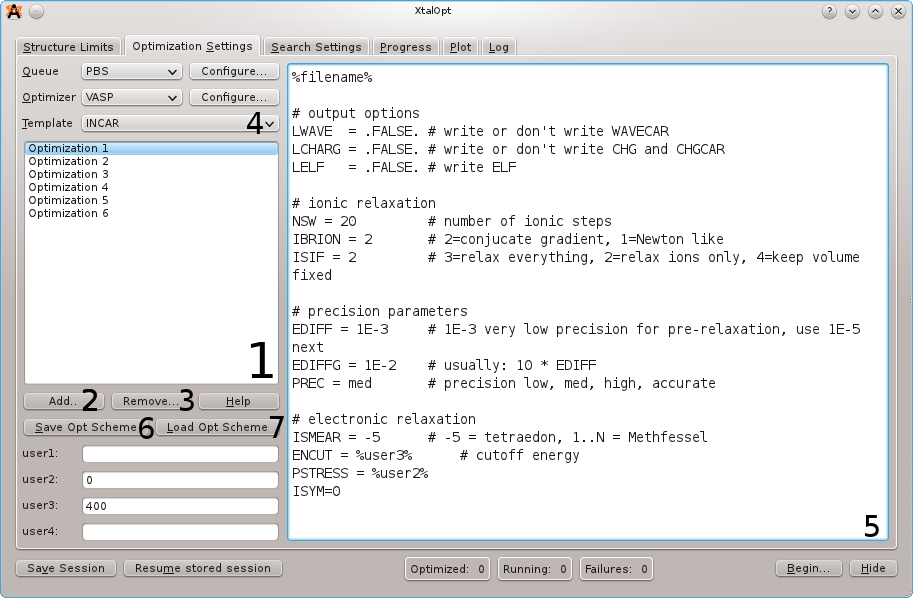
\includegraphics{optschemes-numberededitor.png}
\caption{width=}
\end{DoxyImage}


We will use the above screenshot as we describe the process of creating, saving, and loading optimization schemes. The numbers indicate\-:


\begin{DoxyEnumerate}
\item List of optimization steps
\item Button to add new optimization step
\item Button to remove current optimization step
\item Template selection menu
\item Template editor
\item Button to save current optimization scheme to file
\item Button to load optimization scheme from file
\end{DoxyEnumerate}\hypertarget{optschemes_gui-list}{}\subsection{Optimization step list}\label{optschemes_gui-list}
This list shows the currently available optimization steps in the order that they will be performed. The optstep that is currently selected for editing is highlighted, and the editable optstep can be selected by clicking the appropriate entry.\hypertarget{optschemes_gui-add}{}\subsection{Add new optimization step}\label{optschemes_gui-add}
Clicking this button will append a new optimization step to the optstep list. The new optstep's templates will be copies of the currently selected optstep's templates.\hypertarget{optschemes_gui-rem}{}\subsection{Remove current optimization step}\label{optschemes_gui-rem}
Click this button to delete the currently selected optimization step.\hypertarget{optschemes_gui-tselect}{}\subsection{Select template}\label{optschemes_gui-tselect}
This menu contains the filenames of the templates that are required by the currently selected queuing system (e.\-g. P\-B\-S, S\-G\-E, local...) and optimizer. The currently selected template is displayed in the template editor, and selecting a different template will update the editor.\hypertarget{optschemes_gui-editor}{}\subsection{Template editor}\label{optschemes_gui-editor}
This text editor is used to view and edit the currently selected template for the current optstep.\hypertarget{optschemes_gui-save}{}\subsection{Save scheme}\label{optschemes_gui-save}
This button will prompt for a location to save a .scheme file containing the current optimization step.\hypertarget{optschemes_gui-load}{}\subsection{Resume scheme}\label{optschemes_gui-load}
This button will prompt for an existing .scheme file to load.\hypertarget{optschemes_creating}{}\section{How to build an optimization scheme?}\label{optschemes_creating}
Creating a working scheme from scratch may take some time. We recommend checking the samples/ directory of the source code to obtain sample scheme for each optimizer (see \hyperlink{optschemes_loading}{How to load an optimization scheme?}) and verifying that they are appropriate for the system under consideration before starting a search.

If there is not an appropriate sample, the following prescription may be used to generate your own\-:


\begin{DoxyEnumerate}
\item Generate a random structure of the system under consideration. This may be done by hand, or by running a search just long enough to create the first random generation and saving one of the structures.
\item Create a starting optstep with the desired convergence criteria
\item Manually submit the optimization
\item If the optimization fails\-:
\begin{DoxyEnumerate}
\item First determine why -- if the maximum iterations were exceeded or the optimization was aborted due to a badly performing minimizer, try one of the ideas below. Other optimization problems are beyond the scope of this document.
\item Reduce the convergence criteria of the current trial optstep
\item Remove degrees of freedom, e.\-g. by fixing cell parameters, atomic positions, etc
\item Reduce the accuracy of the calculation in other ways (use a courser integration grid, etc).
\item Change the minimizer (e.\-g. tell the optimizer to use conjugate gradients rather than B\-F\-G\-S, etc)
\end{DoxyEnumerate}
\item Once the optimization succeeds, create another set of input files with the desired convergence criteria for all degrees of freedom.
\item Manually submit the new optimization step. If it fails, try the ideas above until it converges.
\item Once the structure has converged to the desired level of accuracy, try to optimize another randomly generated structure using the optsteps that succeeded previously. Refine them if needed.
\item Once you have successfully optimized enough random structures that you are confident in your method, gather all of the inputs used and write your scheme from them.
\end{DoxyEnumerate}

The scheme may be written by copying each input file into the template editor (with the appropriate optstep and template selected, of course) and replacing the structure-\/specific information with the appropriate keywords. Click the \char`\"{}\-Help\char`\"{} button for the complete list of keywords.

We have found that the optimization schemes are surprisingly transferable within an optimizer, so once you have a working optimization scheme for a given optimization code only minor tweaks (usually to the energy cutoffs, etc ) are necessary to use it on a different chemical system.\hypertarget{optschemes_saving}{}\section{How to save an optimization scheme for later?}\label{optschemes_saving}
Once you have written your optimization scheme, you will want to save it for fast retrieval later (otherwise you will need to copy/paste and edit all of the templates again!). To save, simply click the \char`\"{}\-Save Opt
\-Scheme\char`\"{} button and enter an appropriate filename with an extension of .scheme.\hypertarget{optschemes_loading}{}\section{How to load an optimization scheme?}\label{optschemes_loading}
Loading an optimization is quite simple -- just click the \char`\"{}\-Load Opt
\-Scheme\char`\"{} button and select the .scheme file you wish to load. This will also update the current queuing system and optimizer to those specified by the scheme.\hypertarget{optschemes_format}{}\section{What is saved?}\label{optschemes_format}
The optimization scheme files contain more than just the templates for each optstep. They also store queue and optimizer specific settings. This is useful for storing configuration options for different clusters along with the scheme. Note that although Xtal\-Opt will prompt for an S\-S\-H password if needed, it is {\bfseries N\-O\-T} stored in the scheme file.\hypertarget{optschemes_suggest}{}\section{Suggestions for optimization schemes}\label{optschemes_suggest}
\hypertarget{optschemes_sug-xtal}{}\subsection{Crystals (\-Xtal\-Opt)}\label{optschemes_sug-xtal}
The following list describes the optimization steps used in the samples/vasp-\/xtalopt.\-scheme file distributed with the Xtal\-Opt source code\-:
\begin{DoxyEnumerate}
\item Fix unit cell, only optimize atomic coordinates. A very loose convergence criterion is used, and the number of K\-P\-O\-I\-N\-Ts is kept small.
\item The cell volume is fixed, but atomic positions and cell parameters are allowed to vary. The convergence criteria is the same as before, as is the K\-P\-O\-I\-N\-T grid.
\item All degrees of freedom are considered using the same convergence criteria as before, but with a finer K\-P\-O\-I\-N\-T grid.
\item Same as before, but with a stricter convergence criteria.
\item Same as before, but with a stricter convergence criteria and more K\-P\-O\-I\-N\-Ts.
\item Same as before, but with more K\-P\-O\-I\-N\-Ts.
\end{DoxyEnumerate}

This is only one of many possible optimization schemes that may work for crystals. It may need to be modified to work for your particular system. 
\chapter{Angle correction in Xtal\-Opt}
\label{fixAngles}
\hypertarget{fixAngles}{}
 Prior to optimization, the structure's lattice is adjusted so that all angles are between $60^\circ$ and $120^\circ$; by a process similar to that described by Oganov et al. in their 2008 paper. The following transformations are applied to all combinations of the three lattice vectors\-:

If both conditions \begin{eqnarray} \left| \arccos\left(\frac{\vec{v_i}\cdot \vec{v_j}} {||\vec{v_i}||\,||\vec{v_j}||} \right) - \pi \right| &> \frac{\pi}{3} \mbox{\ ,\ and\ } ||\vec{v_i}|| &\geq ||\vec{v_j}|| \end{eqnarray}

are true, the cell should be transformed. To do this, the vector $\vec{v_i}$ is replaced by the vector $\vec{v_i'}$, defined as

\[ \vec{v_i'} = \vec{v_i} - \mbox{ceil}\left(\left|\frac{\vec{v_i}\cdot \vec{v_j}} {||\vec{v_j}||^2}\right|\right)\mbox{sign}(\vec{v_i}\cdot \vec{v_j})\vec{v_j} \]

This transformation adds a vector $\vec{a} = \pm n \vec{v_j}$ that is parallel to $\vec{v_j}$ with length that is an integer multiple of $||\vec{v_j}||$. The multiplier $n$ is defined as the next highest integer from the absolute value of the scalar projection of $\vec{v_i}$ on $\vec{v_j}$ divided by the length of $\vec{v_j}$ $n = \mbox{ceil}\left(\left(\left|\,\vec{v_i}\cdot \vec{v_j}/ ||\vec{v_j}||\,\right|\right)/||\vec{v_j}||\right)$)\}. The sign of $n\vec{v_j}$ from is determined by $-\mbox{sign}(\vec{v_i}\cdot\vec{v_j})$, resulting in the transformation equation above. For clarification, see the preceeding image.

These equations differ somewhat from those provided by Oganov et al., since the above equations apply to arbitrary length vectors, while those published for Oganov's U\-S\-P\-E\-X code seem to only be applicable to unit vectors.

Atomic coordinates are stored in Cartesian form before the lattice transformation to maintain the structure's atomic configuration. After the new angles are set, the atoms are adjusted so that they lie within the new cell by adding or subtracting 1 from the new fractional coordinates. 
\chapter{Saving and Resuming Sessions in Xtal\-Opt}
\label{xo_saveresume}
\hypertarget{xo_saveresume}{}
\hypertarget{xo_saveresume_sr_contents}{}\section{Contents}\label{xo_saveresume_sr_contents}

\begin{DoxyItemize}
\item \hyperlink{xo_saveresume_sr_saving}{How to save your session}
\item \hyperlink{xo_saveresume_sr_resuming}{How to resume your session}
\end{DoxyItemize}

 
\begin{DoxyImageNoCaption}
  \mbox{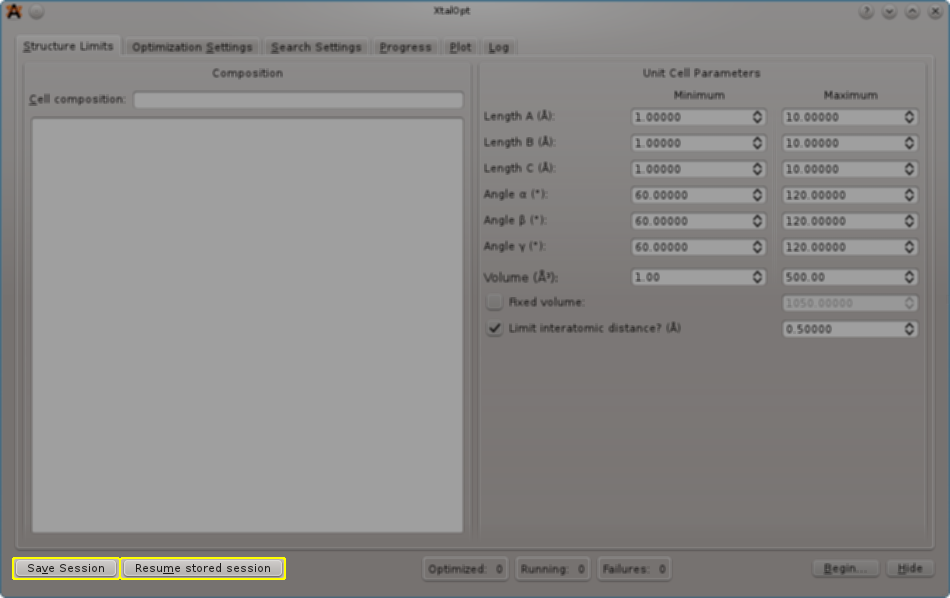
\includegraphics[width=\textwidth]{xo-saveresume.png}}
\end{DoxyImageNoCaption}
\hypertarget{xo_saveresume_sr_saving}{}\section{How to save your session}\label{xo_saveresume_sr_saving}
Xtal\+Opt will write a small file named xtalopt.\+state to its working directory that contains the information necessary to resume the session at a later time. The file can be rewritten manually by clicking the \char`\"{}\+Save Session\char`\"{} button highlighted above, and Xtal\+Opt will automatically save the session every time a structure is updated.

Xtal\+Opt will also write a file \char`\"{}structure.\+state\char`\"{} in each candidate structure\textquotesingle{}s directory. This file stores Xtal\+Opt-\/specific information about the structure.\hypertarget{xo_saveresume_sr_resuming}{}\section{How to resume your session}\label{xo_saveresume_sr_resuming}
To resume a session, simply click \char`\"{}\+Resume stored session\char`\"{} (highlighted above) and select the xtalopt.\+state file in the working directory of the session you would like to resume. Xtal\+Opt will then begin to load the structures and search parameters. You can monitor the progress with the progress bar that appears at the bottom of the window.

While the structures are loading, you may encounter errors that say\+:

\begin{DoxyVerb}Error, no (or not appropriate for [OPTIMIZER]) xtal data in [DIRECTORY].

This could be a result of resuming a structure that has not yet done
any local optimizations. If so, safely ignore this message.
\end{DoxyVerb}


As mentioned in the message, these can typically be ignored if it only happens for a handful of structures. This occurs when a structure has been generated in Xtal\+Opt, but it has not completed any geometry optimization so there are no output files from which to load the geometry. If it happens for a significant number of structures (or structures that are known to have completed at least one geometry optimization step), the output files from the optimizer may be missing or corrupt.

After resuming a session, Xtal\+Opt will ask if you would like to continue the search or enter read-\/only mode. Read-\/only mode will not generate new structures or submit geometry optimizations.

\begin{DoxyNote}{Note}
If you are considering resuming a read-\/only session, take a look at the results.\+txt file in the working directory. It contains a list of all structures, sorted by enthalpy, with additional useful information. This can save some time when trying to locate the most stable structure of a old search.
\end{DoxyNote}
The working directories for Xtal\+Opt are relocatable, meaning that the directory containing xtalopt.\+state and the \mbox{[}gen\mbox{]}x\mbox{[}id\mbox{]} structure folders may be moved, tarred, zipped, etc. and still be resumed at a later time from a different location on the filesystem, or even a different computer. 
\chapter{Xtal\-Opt Tutorial}
\label{tut-xo}
\hypertarget{tut-xo}{}
\hypertarget{tut-xo_Contents}{}\section{Contents}\label{tut-xo_Contents}

\begin{DoxyItemize}
\item \hyperlink{tut-xo_launch}{Launch Xtal\+Opt}
\item \hyperlink{tut-xo_init}{Enter composition and restraints}
\item \hyperlink{tut-xo_opt}{Optimizer setup}
\begin{DoxyItemize}
\item \hyperlink{tut-xo_vasp-opt}{V\+A\+S\+P}
\item \hyperlink{tut-xo_gulp-opt}{G\+U\+L\+P}
\item \hyperlink{tut-xo_pwscf-opt}{P\+Wscf}
\item \hyperlink{tut-xo_castep-opt}{C\+A\+S\+T\+E\+P}
\item \hyperlink{tut-xo_siesta-opt}{S\+I\+E\+S\+T\+A}
\end{DoxyItemize}
\item \hyperlink{tut-xo_qisetup}{Queue setup}
\begin{DoxyItemize}
\item \hyperlink{tut-xo_remotepbs}{Using a remote P\+B\+S cluster}
\item \hyperlink{tut-xo_remotesge}{Using a remote S\+G\+E cluster}
\item \hyperlink{tut-xo_remoteslurm}{Using a remote S\+L\+U\+R\+M cluster}
\item \hyperlink{tut-xo_remotelsf}{Using a remote L\+S\+F cluster}
\item \hyperlink{tut-xo_remotell}{Using a remote Load\+Leveler cluster}
\item \hyperlink{tut-xo_localqi}{Running optimations locally}
\end{DoxyItemize}
\item \hyperlink{tut-xo_files}{What is written to the local directory?}
\item \hyperlink{tut-xo_search-set}{Search Settings}
\item \hyperlink{tut-xo_begin}{\char`\"{}\+Begin\char`\"{}}
\item \hyperlink{tut-xo_prog-mon}{Monitor progress}
\begin{DoxyItemize}
\item \hyperlink{tut-xo_trends}{View trends}
\end{DoxyItemize}
\end{DoxyItemize}\hypertarget{tut-xo_launch}{}\section{Launch Xtal\+Opt}\label{tut-xo_launch}
Open avogadro, go to the \char`\"{}\+Extensions\char`\"{} menu and select \char`\"{}\+Xtal\+Opt\char`\"{}.\hypertarget{tut-xo_init}{}\section{Enter composition and restraints}\label{tut-xo_init}
 
\begin{DoxyImageNoCaption}
  \mbox{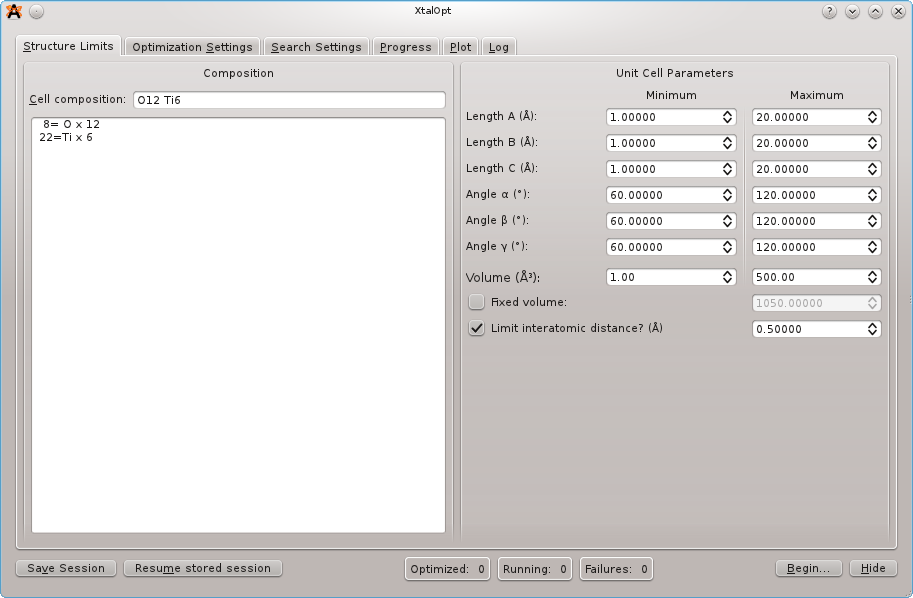
\includegraphics[width=\textwidth]{struct-lim.png}}
\end{DoxyImageNoCaption}


The interface opens to the \char`\"{}\+Structure Limits\char`\"{} tab, shown above. We will use a 6 formula unit supercell of titanium dioxide for this tutorial, so enter \char`\"{}\+Ti6 O12\char`\"{} for the cell composition. We will assume that we know nothing about the system and use very loose restraints. Set all cell length minima to 1 angstrom and maxima to 20 angstrom. Constrain the angles to be between 60 and 120 degrees, and the volume from between 1 and 500 cubic angstrom. Specify a minimum interatomic distance of 0.\+5 angstrom. (Note that due to the angle adjustment described in the C\+P\+C 2010 publication, 60-\/120 degrees is the largest range of cell angles that Xtal\+Opt will generate.)\hypertarget{tut-xo_opt}{}\section{Optimizer setup}\label{tut-xo_opt}
Xtal\+Opt currently supports the \hyperlink{tut-xo_vasp-opt}{V\+A\+S\+P}, \hyperlink{tut-xo_gulp-opt}{G\+U\+L\+P}, \hyperlink{tut-xo_pwscf-opt}{P\+Wscf}, \hyperlink{tut-xo_castep-opt}{C\+A\+S\+T\+E\+P}, and \hyperlink{tut-xo_siesta-opt}{S\+I\+E\+S\+T\+A} codes for performing geometry optimizations. Each is detailed in its own section below.\hypertarget{tut-xo_vasp-opt}{}\subsection{V\+A\+S\+P}\label{tut-xo_vasp-opt}
 
\begin{DoxyImageNoCaption}
  \mbox{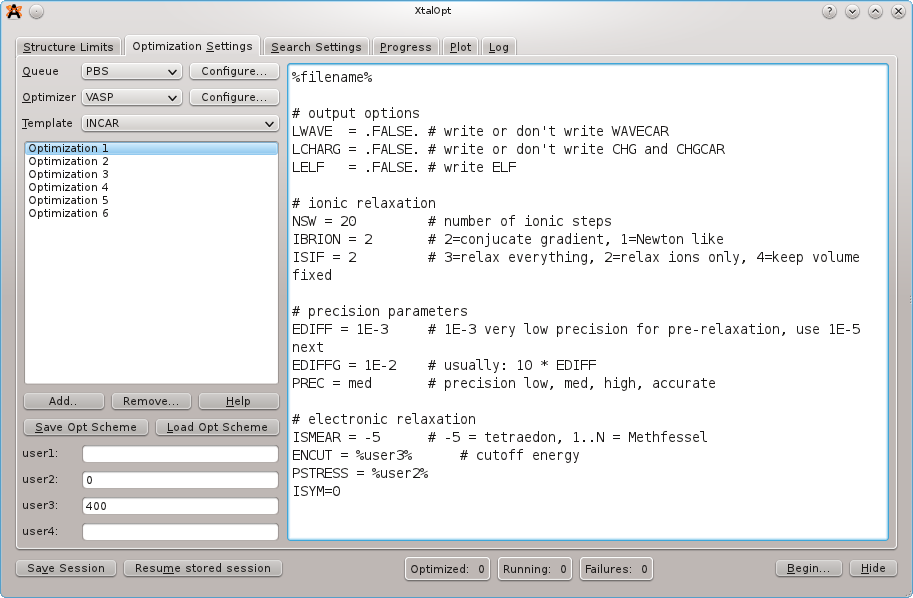
\includegraphics[width=\textwidth]{opt-set-vasp.png}}
\end{DoxyImageNoCaption}


On the next tab, load the optimization scheme by clicking the \char`\"{}\+Load
\+Opt Scheme\char`\"{} button and selecting the \char`\"{}samples/vasp-\/xtalopt.\+scheme\char`\"{} file that is distributed with the source code. If you do not have a copy of the source code, the scheme file can be obtained by clicking the \href{http://xtalopt.github.io/samples/vasp-xtalopt.scheme}{\tt here}.

For more details on optimization schemes, see \hyperlink{optschemes}{Optimization Schemes}.

After loading the optimization scheme, Xtal\+Opt will prompt for the P\+O\+T\+C\+A\+R files to use. Select files appropriated for the prompted atom. Xtal\+Opt will construct the P\+O\+T\+C\+A\+R files on the local computer, and then copy them over to the cluster when the calculation is submitted. It is necessary to have the V\+A\+S\+P P\+O\+T\+C\+A\+R files for each atomic species located somewhere on the local computer. See the V\+A\+S\+P manual for information on obtaining the P\+O\+T\+C\+A\+R files.

Take a moment to look through each file for each optimization step. Notice that the I\+N\+C\+A\+R template includes two user-\/specified values, \%user2\% and \%user3\% for the external pressure and the energy cutoff, respectively. By entering appropriate values in the \char`\"{}user2\+:\char`\"{} and \char`\"{}user3\+:\char`\"{} fields on the left, it is easy to update these values for all optimization steps.

Notice the other \%keyword\% values in the job.\+pbs templates. These are used to enter information that is specific to a search or structure when the actual input files are written prior to job submission. Click the \char`\"{}\+Help\char`\"{} button for a full listing of the available keywords.

Xtal\+Opt expects V\+A\+S\+P to use the default filenames, mainly P\+O\+S\+C\+A\+R, C\+O\+N\+T\+C\+A\+R, and O\+U\+T\+C\+A\+R.

\hyperlink{tut-xo_qisetup}{Skip to next section.}\hypertarget{tut-xo_gulp-opt}{}\subsection{G\+U\+L\+P}\label{tut-xo_gulp-opt}
 
\begin{DoxyImageNoCaption}
  \mbox{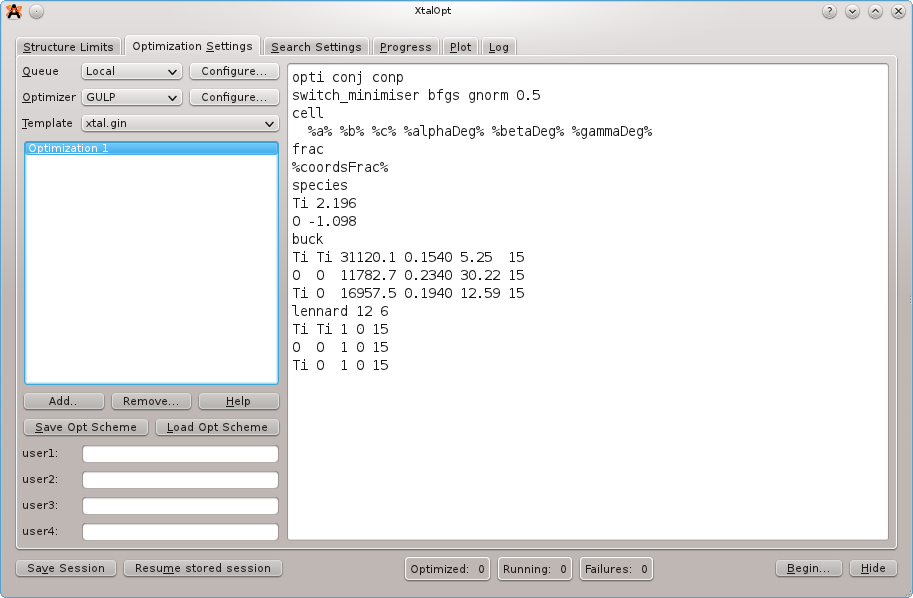
\includegraphics[width=\textwidth]{opt-set-gulp.png}}
\end{DoxyImageNoCaption}


On the next tab we choose G\+U\+L\+P for the local optimizer and enter a template for G\+U\+L\+P to use. Select \char`\"{}\+G\+U\+L\+P\char`\"{} as the \char`\"{}\+Optimizer\char`\"{} and \char`\"{}xtal.\+gin\char`\"{} as \char`\"{}\+Template\char`\"{}. Next, fill out the text field on the right with the following template\+: 
\begin{DoxyCode}
opti conj conp
switch\_minimiser bfgs gnorm 0.5
cell
  %a% %b% %c% %alphaDeg% %betaDeg% %gammaDeg%
frac
%coordsFrac%
species
Ti 2.196
O -1.098
buck
Ti Ti 31120.1 0.1540 5.25  15
O  O  11782.7 0.2340 30.22 15
Ti O  16957.5 0.1940 12.59 15
lennard 12 6
Ti Ti 1 0 15
O  O  1 0 15
Ti O  1 0 15
\end{DoxyCode}


Alternatively, one can load the scheme file distributed with the source code under samples/gulp-\/\+Ti\+O-\/xtalopt.\+scheme. If the source code is not available, the scheme file can be obtained by clicking \href{http://xtalopt.github.io/samples/gulp-TiO-xtalopt.scheme}{\tt here}.

For more details on optimization schemes, see \hyperlink{optschemes}{Optimization Schemes}.

Note the \char`\"{}\%\char`\"{} surrounding various keywords. These will be replaced by the structure-\/specific data when the optimizer is invoked for each structure. Click \char`\"{}\+Help\char`\"{} to view all of the keywords available. The number of optimization steps can be modified with the \char`\"{}\+Add/\+Resume\char`\"{} buttons. The \char`\"{}user\char`\"{} fields in the lower left corner allow users to specify their own keyword/value pairs, which is useful for making changes to multiple optimization steps at once. We will only be using one optimization step in this tutorial.

Xtal\+Opt expects G\+U\+L\+P to use the following filenames\+:


\begin{DoxyCode}
gulp < xtal.gin > xtal.got
\end{DoxyCode}


\hyperlink{tut-xo_qisetup}{Skip to next section.}\hypertarget{tut-xo_pwscf-opt}{}\subsection{P\+Wscf}\label{tut-xo_pwscf-opt}
 
\begin{DoxyImageNoCaption}
  \mbox{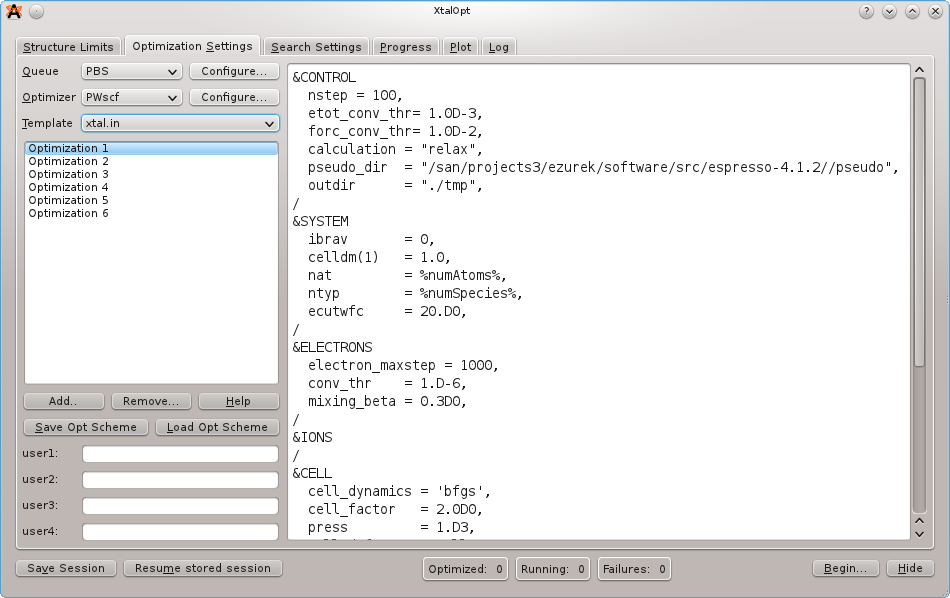
\includegraphics[width=\textwidth]{opt-set-pwscf.png}}
\end{DoxyImageNoCaption}


On the next tab, load the optimization scheme that is distributed with the source code under the samples/ directory. The scheme that we want is named \char`\"{}pwscf-\/xtalopt.\+scheme\char`\"{}. If the source code is not available, the scheme file can be obtained by clicking the \char`\"{}\+Original Format\char`\"{} link at the bottom of the page \href{http://xtalopt.github.io/samples/pwscf-xtalopt.scheme}{\tt here}.

For more details on optimization schemes, see \hyperlink{optschemes}{Optimization Schemes}.

Each P\+Wscf input file will need to be edited to specify\+:
\begin{DoxyEnumerate}
\item The pseudo\+\_\+dir containing the pseudopotential files on the remote cluster, and
\item The pseudopotentials for each atom (under A\+T\+O\+M\+I\+C\+\_\+\+S\+P\+E\+C\+I\+E\+S)
\end{DoxyEnumerate}

Take a moment to look through each file for each optimization step.

Notice the \%keyword\% values in the job.\+pbs templates. These are used to enter information that is specific to a search or structure when the actual input files are written prior to job submission. Click the \char`\"{}\+Help\char`\"{} button for a full listing of the available keywords.

Be aware that every P\+Wscf/\+C\+A\+S\+T\+E\+P installation is different, and it is almost certain that the job.\+pbs file included with this scheme will not work on any cluster other than the Zurek group\textquotesingle{}s \char`\"{}parity\char`\"{} cluster at S\+U\+N\+Y Buffalo\textquotesingle{}s Center for Computational Resources. It may take some experimentation to get jobs to submit successfully, and you may need to contact the mantainers of the cluster for assistance for information about M\+P\+I, executable locations, etc. Perhaps the easiest method to find the correct P\+B\+S script is to run some trial submissions by hand, and then replace the structure/search specific information with the appropriate keywords once a working script has been generated.

Xtal\+Opt expects P\+Wscf to use the following filenames\+:


\begin{DoxyCode}
pw.x < xtal.in > xtal.out
\end{DoxyCode}


\hyperlink{tut-xo_qisetup}{Skip to next section.}\hypertarget{tut-xo_castep-opt}{}\subsection{C\+A\+S\+T\+E\+P}\label{tut-xo_castep-opt}
 
\begin{DoxyImageNoCaption}
  \mbox{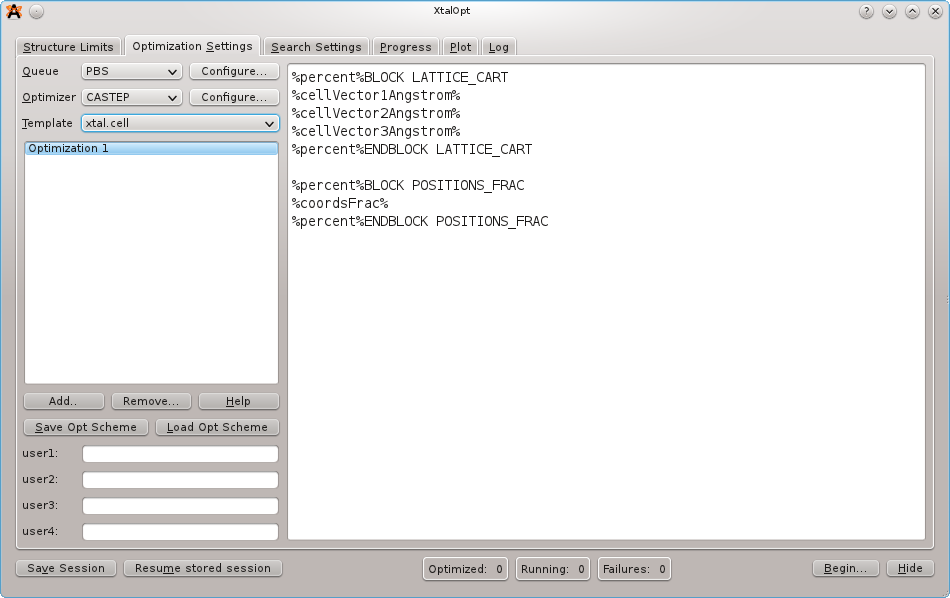
\includegraphics[width=\textwidth]{opt-set-castep.png}}
\end{DoxyImageNoCaption}


On the next tab, load the optimization scheme that is distributed with the source code under the samples/ directory. The scheme that we want is named \char`\"{}castep-\/xtalopt.\+scheme\char`\"{}. If the source code is not available, the scheme file can be obtained by clicking the \char`\"{}\+Original Format\char`\"{} link at the bottom of the page \href{http://xtalopt.github.io/samples/castep-xtalopt.scheme}{\tt here}.

For more details on optimization schemes, see \hyperlink{optschemes}{Optimization Schemes}.

It is important to note that C\+A\+S\+T\+E\+P input files require the \char`\"{}\%\char`\"{} character to define blocks. The percent character is special in the Xtal\+Opt input template parser to define keywords (see below). To insert a literal \char`\"{}\%\char`\"{} into the input, use percent\%.

E.\+g. Specification of the fractional coordinate block in the .cell template should look like\+:


\begin{DoxyCode}
%percent%BLOCK POSITIONS\_FRAC
%coordsFrac%
%percent%ENDBLOCK POSITIONS\_FRAC
\end{DoxyCode}


Take a moment to look through each file for each optimization step.

Notice the \%keyword\% values in the job.\+pbs templates. These are used to enter information that is specific to a search or structure when the actual input files are written prior to job submission. Click the \char`\"{}\+Help\char`\"{} button for a full listing of the available keywords.

Be aware that every P\+Wscf/\+C\+A\+S\+T\+E\+P installation is different, and it is almost certain that the job.\+pbs file included with this scheme will not work on any cluster other than the Zurek group\textquotesingle{}s \char`\"{}parity\char`\"{} cluster at S\+U\+N\+Y Buffalo\textquotesingle{}s Center for Computational Resources. It may take some experimentation to get jobs to submit successfully, and you may need to contact the mantainers of the cluster for assistance for information about M\+P\+I, executable locations, etc. Perhaps the easiest method to find the correct P\+B\+S script is to run some trial submissions by hand, and then replace the structure/search specific information with the appropriate keywords once a working script has been generated.

Xtal\+Opt expects C\+A\+S\+T\+E\+P to use the following filenames\+:


\begin{DoxyCode}
\textcolor{preprocessor}{# XtalOpt will write xtal.cell, xtal.param}
castep xtal
\textcolor{preprocessor}{# CASTEP will create xtal.castep}
\end{DoxyCode}


\hyperlink{tut-xo_qisetup}{Skip to next section.}\hypertarget{tut-xo_siesta-opt}{}\subsection{S\+I\+E\+S\+T\+A}\label{tut-xo_siesta-opt}
 
\begin{DoxyImageNoCaption}
  \mbox{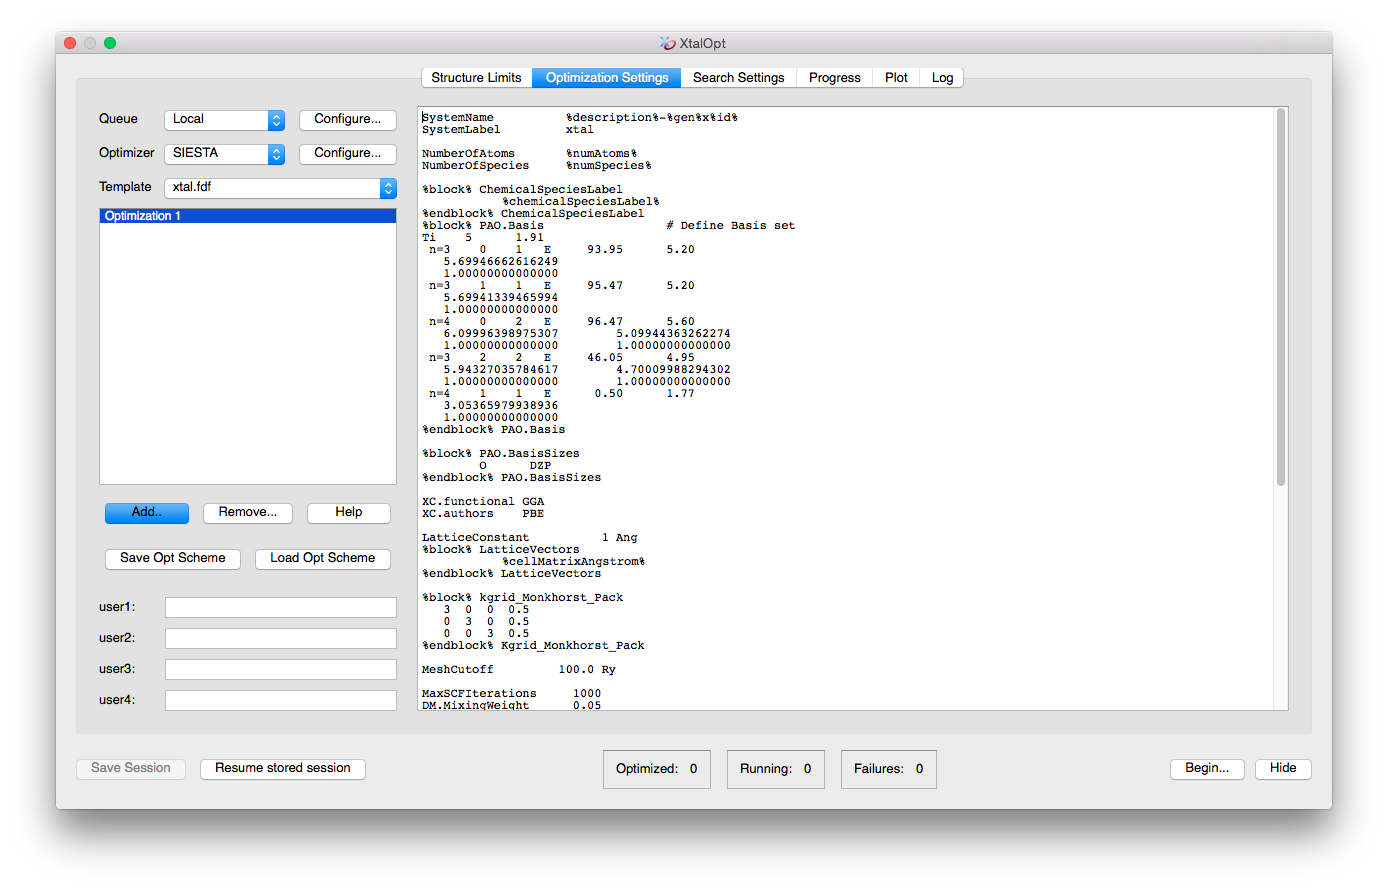
\includegraphics[width=\textwidth]{opt-set-siesta.png}}
\end{DoxyImageNoCaption}


On the next tab we choose G\+U\+L\+P for the local optimizer and enter a template for S\+I\+E\+S\+T\+A to use. Select \char`\"{}\+S\+I\+E\+S\+T\+A\char`\"{} as the \char`\"{}\+Optimizer\char`\"{} and \char`\"{}xtal.\+fdf\char`\"{} as \char`\"{}\+Template\char`\"{}.

Next, fill out the text field on the right with the following template\+:


\begin{DoxyCode}
SystemName          %description%-%gen%x%\textcolor{keywordtype}{id}%
SystemLabel         xtal

NumberOfAtoms       %numAtoms%
NumberOfSpecies     %numSpecies%

%block% ChemicalSpeciesLabel
%chemicalSpeciesLabel%
%endblock% ChemicalSpeciesLabel

%block% PAO.Basis                 # Define Basis set
Ti    5      1.91
 n=3    0    1   E     93.95      5.20
   5.69946662616249
   1.00000000000000
 n=3    1    1   E     95.47      5.20
   5.69941339465994
   1.00000000000000
 n=4    0    2   E     96.47      5.60
   6.09996398975307        5.09944363262274
   1.00000000000000        1.00000000000000
 n=3    2    2   E     46.05      4.95
   5.94327035784617        4.70009988294302
   1.00000000000000        1.00000000000000
 n=4    1    1   E      0.50      1.77
   3.05365979938936
   1.00000000000000
%endblock% PAO.Basis

%block% PAO.BasisSizes
        O      DZP
%endblock% PAO.BasisSizes

XC.functional GGA
XC.authors    PBE

LatticeConstant          1 Ang
%block% LatticeVectors
%cellMatrixAngstrom%
%endblock% LatticeVectors

%block% kgrid\_Monkhorst\_Pack
   3  0  0  0.5
   0  3  0  0.5
   0  0  3  0.5
%endblock% Kgrid\_Monkhorst\_Pack

MeshCutoff         100.0 Ry

MaxSCFIterations     1000
DM.MixingWeight      0.05
DM.NumberPulay       3
DM.Tolerance         1.d-4

SolutionMethod       diagon

SpinPolarized   \textcolor{keyword}{true}
LongOutput \textcolor{keyword}{true}

MD.TypeOfRun        cg
MD.NumCGsteps       1000
MD.VariableCell     \textcolor{keyword}{true}
MD.MaxForceTol      0.01 eV/Ang  #0.005 eV/Ang
WriteForces         \textcolor{keyword}{true}
WriteCoorCerius     \textcolor{keyword}{true}
WriteCoorXmol       \textcolor{keyword}{false}
WriteDenchar        \textcolor{keyword}{true}
WriteMullikenPop    1

UseSaveData         \textcolor{keyword}{true}

\textcolor{preprocessor}{#Diag.ParallelOverK true}

AtomicCoordinatesFormat Fractional
%block% AtomicCoordinatesAndAtomicSpecies
%atomicCoordsAndAtomicSpecies%
%endblock% AtomicCoordinatesAndAtomicSpecies
\end{DoxyCode}


Or load the optimization scheme by clicking the \char`\"{}\+Load Opt Scheme\char`\"{} button and selecting the \char`\"{}samples/siesta-\/\+Ti\+O-\/xtalopt.\+scheme\char`\"{} file that is distributed with the source code. If the source code is not available, the scheme file can be obtained by clicking \href{http://xtalopt.github.io/samples/siesta-TiO-xtalopt.scheme}{\tt here}.

For more details on optimization schemes, see \hyperlink{optschemes}{Optimization Schemes}.

After loading the optimization scheme, Xtal\+Opt will prompt for the xtal.\+psf files to use. Select files appropriated for the prompted atom. Xtal\+Opt will copy the individual files over to each structure directory when the calculation is submitted. See the S\+I\+E\+S\+T\+A manual for information on obtaining the .psf files.

Notice the other keyword\% values in the xtal.\+fdf templates. These are used to enter information that is specific to a search or structure when the actual input files are written prior to job submission. Click the \char`\"{}\+Help\char`\"{} button for a full listing of the available keywords.

Xtal\+Opt expects S\+I\+E\+S\+T\+A to use the following filenames\+:


\begin{DoxyPre}siesta < xtal.fdf > xtal.out\end{DoxyPre}
\hypertarget{tut-xo_qisetup}{}\section{Queue setup}\label{tut-xo_qisetup}
Xtal\+Opt currently supports using the \hyperlink{tut-xo_remotepbs}{P\+B\+S}, \hyperlink{tut-xo_remotesge}{S\+G\+E}, \hyperlink{tut-xo_remoteslurm}{S\+L\+U\+R\+M}, \hyperlink{tut-xo_remotelsf}{L\+S\+F}, and \hyperlink{tut-xo_remotell}{Load\+Leveler} queuing systems on remote S\+S\+H-\/accessible clusters, as well as an internal \hyperlink{tut-xo_localqi}{local} queue that manages calculations on the user\textquotesingle{}s workstation. Each queueing interface is detailed in its own section below.\hypertarget{tut-xo_remotepbs}{}\subsection{Using a remote P\+B\+S cluster}\label{tut-xo_remotepbs}
 
\begin{DoxyImageNoCaption}
  \mbox{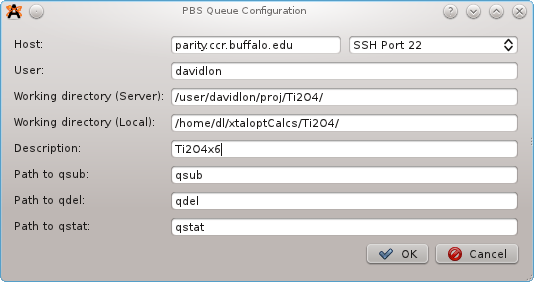
\includegraphics[width=\textwidth]{opt-set-pbs.png}}
\end{DoxyImageNoCaption}


Select \char`\"{}\+P\+B\+S\char`\"{} from the list of Queues, and then click the \char`\"{}\+Configure...\char`\"{} button. A new window will prompt for\+:
\begin{DoxyItemize}
\item host\+: The hostname of the P\+B\+S cluster\textquotesingle{}s head node
\item user\+: The username used to log into the cluster
\item Working directory (Server)\+: A directory that is readable/writable by \char`\"{}user\char`\"{} on the cluster, used when performing optimizations.
\item Working directory (Local)\+: A directory that is readable/writable by the current user on the local computer. This is where the final structures and resume files are written.
\item Description\+: Used for the \%description\% keyword in input templates.
\item Path to qsub\+: Where to find the qsub executable on the remote cluster. Note that if qsub is in the cluster\textquotesingle{}s \$\+P\+A\+T\+H, setting this to just \textquotesingle{}qsub\textquotesingle{} will work.
\item Path to qdel\+: Where to find the qdel executable on the remote cluster. Note that if qdel is in the cluster\textquotesingle{}s \$\+P\+A\+T\+H, setting this to just \textquotesingle{}qdel\textquotesingle{} will work.
\item Path to qstat\+: Where to find the qstat executable on the remote cluster. Note that if qstat is in the cluster\textquotesingle{}s \$\+P\+A\+T\+H, setting this to just \textquotesingle{}qstat\textquotesingle{} will work.
\end{DoxyItemize}

A new template, \char`\"{}job.\+pbs\char`\"{} is added to the list of available templates. This is the job submission script for P\+B\+S. This script should roughly follow this design\+:


\begin{DoxyCode}
\textcolor{preprocessor}{#/bin/bash}
\textcolor{preprocessor}{#PBS -l nodes=1:ppn=8}
\textcolor{preprocessor}{#PBS -o ../%gen%x%id%-%optstep%.out}
\textcolor{preprocessor}{#PBS -e ../%gen%x%id%-%optstep%.err}
\textcolor{preprocessor}{#PBS -N %description%-%gen%x%id%-%optstep%}

\textcolor{preprocessor}{###Include this for XtalOpt scripts!###}
export PBS\_O\_WORKDIR=%rempath%

\textcolor{preprocessor}{# Change to structure's working directory, copy input files to node's scratch dirs:}
\textcolor{keywordflow}{for} node in `cat $PBS\_NODEFILE | sort | uniq`; \textcolor{keywordflow}{do}
rsh $node \textcolor{stringliteral}{"cp $PBS\_O\_WORKDIR/* $PBSTMPDIR/;"};
done

\textcolor{preprocessor}{# Move to the scratch directory}
cd $PBSTMPDIR
echo \textcolor{stringliteral}{"running in directory $PBSTMPDIR"}

\textcolor{preprocessor}{# Set any environment variables needed for the optimizer/MPI here:}

\textcolor{preprocessor}{# Run optimizer, be sure to use the filenames that XtalOpt expects.}
\textcolor{preprocessor}{# See the template menu in XtalOpt and the example templates in the}
\textcolor{preprocessor}{# samples/ directory of the XtalOpt sources.}

\textcolor{preprocessor}{# Don't forget to clean up after MPI if needed!}

\textcolor{comment}{// Print files from each node}
\textcolor{keywordflow}{for} node in `cat $PBS\_NODEFILE | sort | uniq`; \textcolor{keywordflow}{do}
echo \textcolor{stringliteral}{"$node:"}
rsh $node \textcolor{stringliteral}{"ls -l $PBSTMPDIR"}
done
\textcolor{preprocessor}{# Copy back results from master node's scratch directory}
\textcolor{preprocessor}{cp $PBSTMPDIR}\textcolor{comment}{/* $PBS\_O\_WORKDIR/}
\end{DoxyCode}


For more details on optimization schemes, see \hyperlink{optschemes}{Optimization Schemes}.

Be aware that every installation is different, and it is almost certain that the job.\+pbs file included with this scheme will not work on any cluster other than the Zurek group\textquotesingle{}s \char`\"{}parity\char`\"{} cluster at S\+U\+N\+Y Buffalo\textquotesingle{}s Center for Computational Resources. It may take some experimentation to get jobs to submit successfully, and you may need to contact the mantainers of the cluster for assistance or information about M\+P\+I, executable locations, etc. Perhaps the easiest method to find the correct P\+B\+S script is to run some trial submissions by hand, and then replace the structure/search specific information with the appropriate keywords once a working script has been generated.

A handy trick for monitoring jobs outside of Xtal\+Opt is to include the following line in job.\+pbs\+:


\begin{DoxyCode}
\textcolor{preprocessor}{#PBS -N %description%-%gen%x%id%-%optstep%}
\end{DoxyCode}


This will name each job, for example, xtal\+Search-\/3x4-\/2, where xtal\+Search is a user-\/specified description of the search, and 3x4-\/2 means that it is the fourth structure in the third generation running its second optimization step.

\hyperlink{tut-xo_files}{Skip to next section.}\hypertarget{tut-xo_remotesge}{}\subsection{Using a remote S\+G\+E cluster}\label{tut-xo_remotesge}
 
\begin{DoxyImageNoCaption}
  \mbox{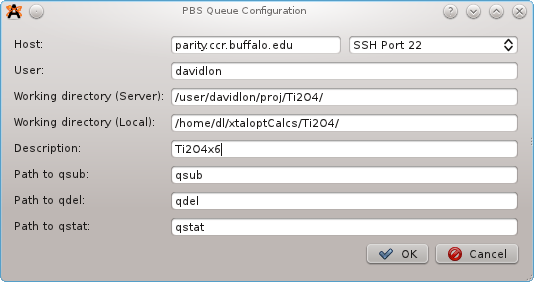
\includegraphics[width=\textwidth]{opt-set-pbs.png}}
\end{DoxyImageNoCaption}
 \begin{DoxyRefDesc}{Todo}
\item[\hyperlink{todo__todo000001}{Todo}]Get screenshots of S\+G\+E config dialog\end{DoxyRefDesc}


Select \char`\"{}\+S\+G\+E\char`\"{} from the list of Queues, and then click the \char`\"{}\+Configure...\char`\"{} button. A new window will prompt for\+:
\begin{DoxyItemize}
\item host\+: The hostname of the S\+G\+E cluster\textquotesingle{}s head node
\item user\+: The username used to log into the cluster
\item Working directory (Server)\+: A directory that is readable/writable by \char`\"{}user\char`\"{} on the cluster, used when performing optimizations.
\item Working directory (Local)\+: A directory that is readable/writable by the current user on the local computer. This is where the final structures and resume files are written.
\item Description\+: Used for the \%description\% keyword in input templates.
\item Path to qsub\+: Where to find the qsub executable on the remote cluster. Note that if qsub is in the cluster\textquotesingle{}s \$\+P\+A\+T\+H, setting this to just \textquotesingle{}qsub\textquotesingle{} will work.
\item Path to qdel\+: Where to find the qdel executable on the remote cluster. Note that if qdel is in the cluster\textquotesingle{}s \$\+P\+A\+T\+H, setting this to just \textquotesingle{}qdel\textquotesingle{} will work.
\item Path to qstat\+: Where to find the qstat executable on the remote cluster. Note that if qstat is in the cluster\textquotesingle{}s \$\+P\+A\+T\+H, setting this to just \textquotesingle{}qstat\textquotesingle{} will work.
\end{DoxyItemize}

\begin{DoxyRefDesc}{Todo}
\item[\hyperlink{todo__todo000002}{Todo}]Get template for job.\+sge scripts\end{DoxyRefDesc}


A new template, \char`\"{}job.\+sge\char`\"{} is added to the list of available templates. This is the job submission script for S\+G\+E. It may take some experimentation to get jobs to submit successfully, and you may need to contact the mantainers of the cluster for assistance or information about M\+P\+I, executable locations, etc. Perhaps the easiest method to find the correct S\+G\+E script is to run some trial submissions by hand, and then replace the structure/search specific information with the appropriate keywords once a working script has been generated.

For more details on optimization schemes, see \hyperlink{optschemes}{Optimization Schemes}.

\hyperlink{tut-xo_files}{Skip to next section.}\hypertarget{tut-xo_remoteslurm}{}\subsection{Using a remote S\+L\+U\+R\+M cluster}\label{tut-xo_remoteslurm}
 
\begin{DoxyImageNoCaption}
  \mbox{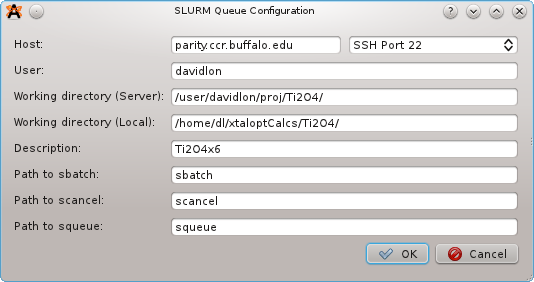
\includegraphics[width=\textwidth]{opt-set-slurm.png}}
\end{DoxyImageNoCaption}


Select \char`\"{}\+S\+L\+U\+R\+M\char`\"{} from the list of Queues, and then click the \char`\"{}\+Configure...\char`\"{} button. A new window will prompt for\+:
\begin{DoxyItemize}
\item host\+: The hostname of the S\+G\+E cluster\textquotesingle{}s head node
\item user\+: The username used to log into the cluster
\item Working directory (Server)\+: A directory that is readable/writable by \char`\"{}user\char`\"{} on the cluster, used when performing optimizations.
\item Working directory (Local)\+: A directory that is readable/writable by the current user on the local computer. This is where the final structures and resume files are written.
\item Description\+: Used for the \%description\% keyword in input templates.
\item Path to sbatch\+: Where to find the sbatch executable on the remote cluster. Note that if sbatch is in the cluster\textquotesingle{}s \$\+P\+A\+T\+H, setting this to just \textquotesingle{}sbatch\textquotesingle{} will work.
\item Path to scancel\+: Where to find the scancel executable on the remote cluster. Note that if scancel is in the cluster\textquotesingle{}s \$\+P\+A\+T\+H, setting this to just \textquotesingle{}scancel\textquotesingle{} will work.
\item Path to squeue\+: Where to find the squeue executable on the remote cluster. Note that if squeue is in the cluster\textquotesingle{}s \$\+P\+A\+T\+H, setting this to just \textquotesingle{}squeue\textquotesingle{} will work.
\end{DoxyItemize}

\begin{DoxyRefDesc}{Todo}
\item[\hyperlink{todo__todo000003}{Todo}]Get template for job.\+slurm scripts\end{DoxyRefDesc}


A new template, \char`\"{}job.\+slurm\char`\"{} is added to the list of available templates. This is the job submission script for S\+L\+U\+R\+M. It may take some experimentation to get jobs to submit successfully, and you may need to contact the mantainers of the cluster for assistance or information about M\+P\+I, executable locations, etc. Perhaps the easiest method to find the correct S\+L\+U\+R\+M script is to run some trial submissions by hand, and then replace the structure/search specific information with the appropriate keywords once a working script has been generated.

For more details on optimization schemes, see \hyperlink{optschemes}{Optimization Schemes}.

\hyperlink{tut-xo_files}{Skip to next section.}\hypertarget{tut-xo_remotelsf}{}\subsection{Using a remote L\+S\+F cluster}\label{tut-xo_remotelsf}
 
\begin{DoxyImageNoCaption}
  \mbox{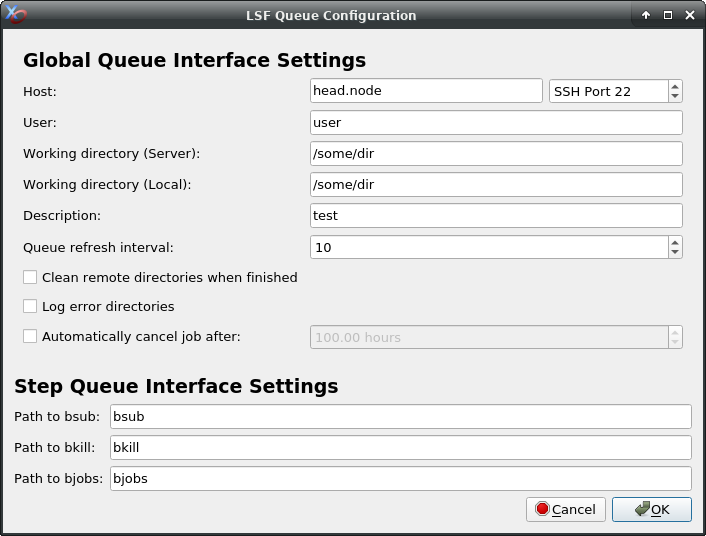
\includegraphics[width=\textwidth]{opt-set-lsf.png}}
\end{DoxyImageNoCaption}


Select \char`\"{}\+L\+S\+F\char`\"{} from the list of Queues, and then click the \char`\"{}\+Configure...\char`\"{} button. A new window will prompt for\+:
\begin{DoxyItemize}
\item host\+: The hostname of the L\+S\+F cluster\textquotesingle{}s head node
\item user\+: The username used to log into the cluster
\item Working directory (Server)\+: A directory that is readable/writable by \char`\"{}user\char`\"{} on the cluster, used when performing optimizations.
\item Working directory (Local)\+: A directory that is readable/writable by the current user on the local computer. This is where the final structures and resume files are written.
\begin{DoxyItemize}
\item Description\+: Used for the description\% keyword in input templates.
\item Path to bsub\+: Where to find the bsub executable on the remote cluster. Note that if bsub is in the cluster\textquotesingle{}s \$\+P\+A\+T\+H, setting this to just \textquotesingle{}bsub\textquotesingle{} will work.
\item Path to bkill\+: Where to find the bkill executable on the remote cluster. Note that if bkill is in the cluster\textquotesingle{}s \$\+P\+A\+T\+H, setting this to just \textquotesingle{}bkill\textquotesingle{} will work.
\item Path to bjobs\+: Where to find the bjobs executable on the remote cluster. Note that if bjobs is in the cluster\textquotesingle{}s \$\+P\+A\+T\+H, setting this to just \textquotesingle{}bjobs\textquotesingle{} will work.
\end{DoxyItemize}
\end{DoxyItemize}

A new template, \char`\"{}job.\+lsf\char`\"{} is added to the list of available templates. This is the job submission script for L\+S\+F. It may take some experimentation to get jobs to submit successfully, and you may need to contact the mantainers of the cluster for assistance or information about M\+P\+I, executable locations, etc. Perhaps the easiest method to find the correct L\+S\+F script is to run some trial submissions by hand, and then replace the structure/search specific information with the appropriate keywords once a working script has been generated.

For more details on optimization schemes, see \hyperlink{optschemes}{Optimization Schemes}.

\hyperlink{tut-xo_files}{Skip to next section.}\hypertarget{tut-xo_remotell}{}\subsection{Using a remote Load\+Leveler cluster}\label{tut-xo_remotell}
 
\begin{DoxyImageNoCaption}
  \mbox{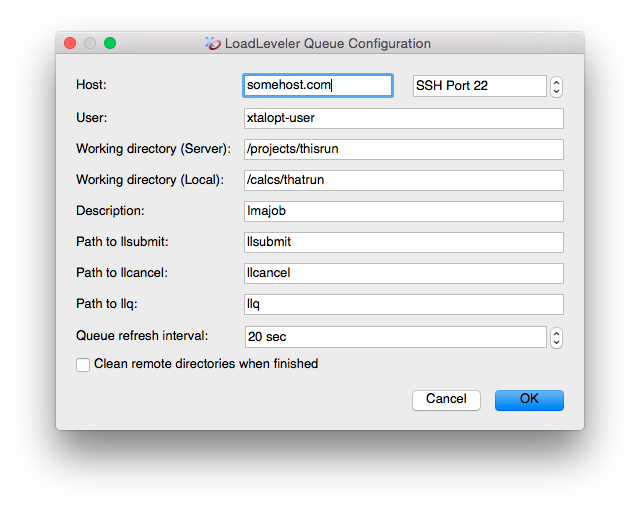
\includegraphics[width=\textwidth]{opt-set-ll.png}}
\end{DoxyImageNoCaption}


Select \char`\"{}\+Load\+Leveler\char`\"{} from the list of Queues, and then click the \char`\"{}\+Configure...\char`\"{} button. A new window will prompt for\+:
\begin{DoxyItemize}
\item host\+: The hostname of the Load\+Leveler cluster\textquotesingle{}s head node
\item user\+: The username used to log into the cluster
\item Working directory (Server)\+: A directory that is readable/writable by \char`\"{}user\char`\"{} on the cluster, used when performing optimizations.
\item Working directory (Local)\+: A directory that is readable/writable by the current user on the local computer. This is where the final structures and resume files are written.
\item Description\+: Used for the description\% keyword in input templates.
\item Path to llsubmit\+: Where to find the llsubmit executable on the remote cluster. Note that if llsubmit is in the cluster\textquotesingle{}s \$\+P\+A\+T\+H, setting this to just \textquotesingle{}llsubmit\textquotesingle{} will work.
\item Path to llcancel\+: Where to find the llcancel executable on the remote cluster. Note that if llcancel is in the cluster\textquotesingle{}s \$\+P\+A\+T\+H, setting this to just \textquotesingle{}llcancel\textquotesingle{} will work.
\item Path to llq\+: Where to find the llq executable on the remote cluster. Note that if llq is in the cluster\textquotesingle{}s \$\+P\+A\+T\+H, setting this to just \textquotesingle{}llq\textquotesingle{} will work.
\end{DoxyItemize}

A new template, \char`\"{}job.\+ll\char`\"{} is added to the list of available templates. This is the job submission script for Load\+Leveler. It may take some experimentation to get jobs to submit successfully, and you may need to contact the mantainers of the cluster for assistance or information about M\+P\+I, executable locations, etc. Perhaps the easiest method to find the correct Load\+Leveler script is to run some trial submissions by hand, and then replace the structure/search specific information with the appropriate keywords once a working script has been generated.

For more details on optimization schemes, see \hyperlink{optschemes}{Optimization Schemes}.

\hyperlink{tut-xo_files}{Skip to next section.}\hypertarget{tut-xo_localqi}{}\subsection{Running optimations locally}\label{tut-xo_localqi}
 
\begin{DoxyImageNoCaption}
  \mbox{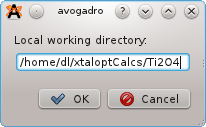
\includegraphics[width=.5\textwidth]{opt-set-local.png}}
\end{DoxyImageNoCaption}


Select \char`\"{}\+Local\char`\"{} from the list of Queues, and then click the configure button. A new window will prompt for\+:
\begin{DoxyItemize}
\item Local working directory\+: A directory that is readable/writable by the current user on the local computer. This is where the final structures and resume files are written.
\end{DoxyItemize}

If the optimizer\textquotesingle{}s executable (vasp, gulp, pw.\+x, castep, etc) is not in your system path, you will need to specify the location of the executable by clicking the \char`\"{}\+Configure...\char`\"{} button next to the optimizer selection menu.

For more details on optimization schemes, see \hyperlink{optschemes}{Optimization Schemes}.\hypertarget{tut-xo_files}{}\section{What is written to the local directory?}\label{tut-xo_files}
A directory for each structure is created at


\begin{DoxyCode}
[Local working directory]/<gen#>x<id#>
\end{DoxyCode}


that will contain input, output, and data files specific to each structure. Two additional files are also written to the local filesystem\+:


\begin{DoxyCode}
[Local working directory]/xtalopt.state
\end{DoxyCode}


which contains save/resume information to continue a session that has been stopped, and


\begin{DoxyCode}
[Local working directory]/results.txt
\end{DoxyCode}


which stores a list of all structures sorted by increasing enthalpy. The latter file is handy for offline analysis, since there is no need to open Xtal\+Opt to find the most stable structures of a previous search.\hypertarget{tut-xo_search-set}{}\section{Search Settings}\label{tut-xo_search-set}
 
\begin{DoxyImageNoCaption}
  \mbox{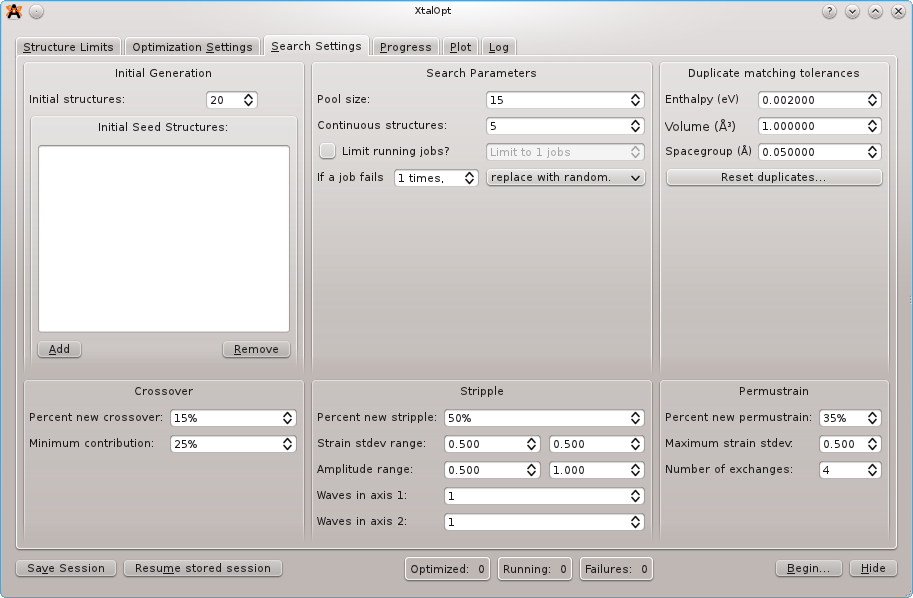
\includegraphics[width=\textwidth]{search-set.png}}
\end{DoxyImageNoCaption}


In the \char`\"{}\+Search Settings\char`\"{} tab, most of the default settings should suffice (See C\+P\+C 2010 publication). We arbitrarily set the initial structures to 20 and the continuous structures to 5, although these may need to be adjusted based on available resources. We will not specify initial seeds, but the option to do so exists on this screen.

It is not neccessary to limit the number of running jobs unless running locally, as the P\+B\+S queue on the cluster will manage job control for us. If running locally, set the job limit no higher than \mbox{[}number of available processor cores\mbox{]} -\/ 1 (e.\+g. for a quadcore processor, allow three jobs to run simultaneously). This allows one core to remain free for the system to run.

There is now a termination criteria called \char`\"{}\+Total Number of Structures\char`\"{} that will end the run once a certain number of strcutures have been produced by Xtal\+Opt.\hypertarget{tut-xo_begin}{}\section{\char`\"{}\+Begin\char`\"{}}\label{tut-xo_begin}

\begin{DoxyImage}
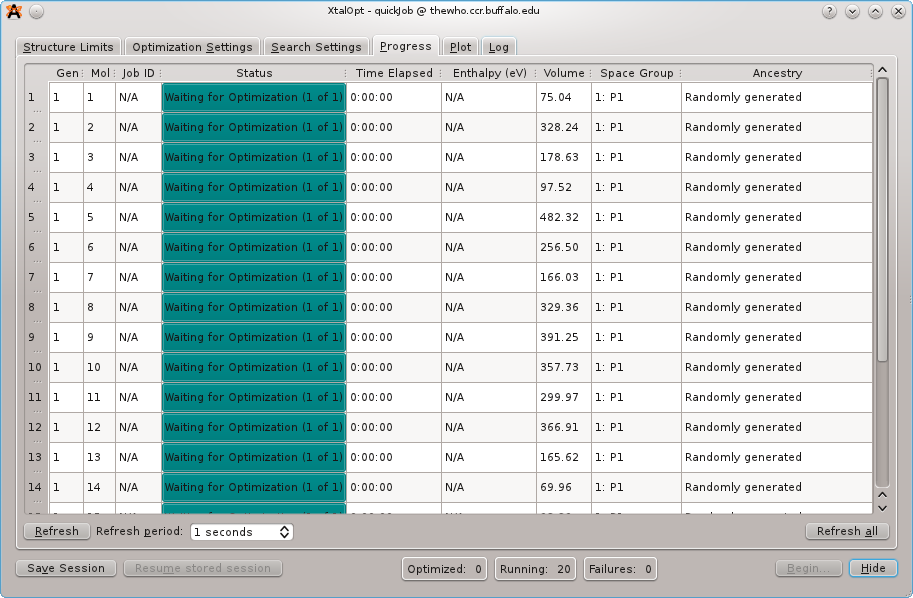
\includegraphics[width=\textwidth]{prog-start.png}
\caption{The ``\+Progress\textquotesingle{}\textquotesingle{} tab immediately after starting a search}
\end{DoxyImage}


Xtal\+Opt has everything it needs to start its search at this point; click the \char`\"{}\+Begin\char`\"{} button in the lower right corner of the application to tell it to start the search algorithm. A progress bar appears as the random first generation is created. Switch to the \char`\"{}\+Progress\char`\"{} tab and 20 entries will appear, all with a status of \char`\"{}\+Waiting for
\+Optimization\char`\"{}. Click \char`\"{}\+Refresh\char`\"{} on this tab to begin the local optimizations. From here, Xtal\+Opt will continue to run without user input, starting new optimizations and generating new structures until it is stopped by the user.\hypertarget{tut-xo_prog-mon}{}\section{Monitor progress}\label{tut-xo_prog-mon}

\begin{DoxyImage}
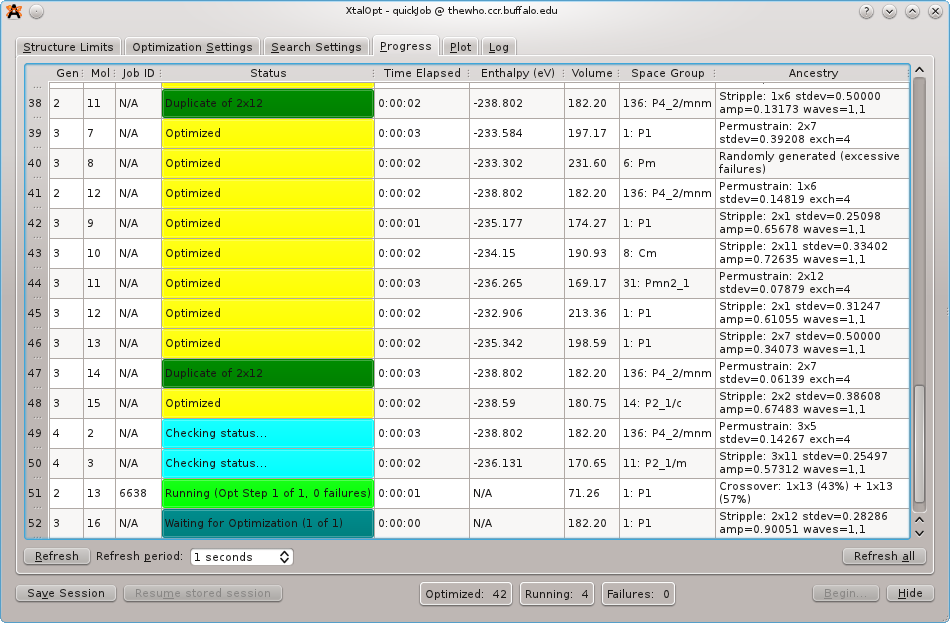
\includegraphics[width=\textwidth]{prog-mon.png}
\caption{The ``\+Progress\textquotesingle{}\textquotesingle{} tab mid-\/run}
\end{DoxyImage}


As Xtal\+Opt performs the search, the progress table continuously updates, providing information about each structure. We see individuals in various stages of completion\+: most are optimized (in blue), structure 2x7 has been automatically marked as a duplicate (dark green) of structure 3x3 and removed from the breeding pool, structure 4x4 is currently undergoing a local optimization (light green), while structure 4x5 is waiting to be optimized (light blue).

Other useful information is displayed about each structure, such as the time spent in optimization, the optimized enthalpy, the cell volume, spacegroup, and each structure\textquotesingle{}s ancestory (i.\+e. parent(s) and parameters for the genetic operator that generated it). A status bar on the bottom of the window shows the number of structures that are optimized, running, and failing at any given time. This information is visible regardless of which tab is currently being viewed.

An additional feature of the progress table is the ability to immediately visualize any of the individuals in the Avogadro main window -- simply clicking on a row in this table will display the three-\/dimensional structure in Avogadro, where it can be visualized, modified, or exported. If the user would like to add a bit of \char`\"{}intelligent design\char`\"{} to the evolutionary process, a structure can be modified and then resubmitted using a context (right-\/click) menu from the progress table. The context menu provides tools to (un)kill a structure, resubmit for local optimization at an arbitrary optimization step, or replace a problematic structure with a new, random individual.

Three additional buttons found near the \char`\"{}\+Refresh All\char`\"{} button in this tab are also available. The \char`\"{}\+Print Results File\char`\"{} button generates a run-\/results.\+txt file that lists all of the information about each structure in order of generation and structure number (As compared to the results.\+txt file which ranks the structures). The \char`\"{}\+Remove Extra Files\char`\"{} button is used for V\+A\+S\+P runs. It removes any extraneous files in each local subdirectory in order to reduce disk usage. Files kept are structure.\+state, P\+O\+T\+C\+A\+R, C\+O\+N\+T\+C\+A\+R, O\+S\+Z\+I\+C\+A\+R, job.\+slurm and O\+U\+T\+C\+A\+R. Finally, the \char`\"{}\+Rank All\char`\"{} button ranks all currently optimized structures and exports them to a subdirectory (Ranked) in two forms (depending on the optimizer)\+: P\+O\+S\+C\+A\+R/.got and .cif. Each can be found in separate directories. (Only works for G\+U\+L\+P and V\+A\+S\+P runs currently).\hypertarget{tut-xo_trends}{}\subsection{View trends}\label{tut-xo_trends}

\begin{DoxyImage}
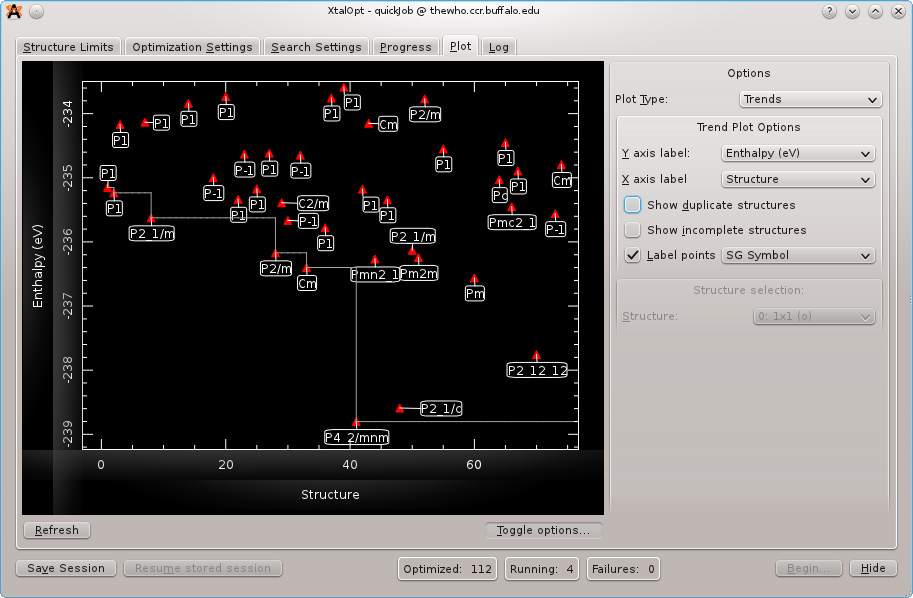
\includegraphics[width=\textwidth]{trend-view.png}
\caption{The ``\+Plot\textquotesingle{}\textquotesingle{} tab mid-\/run displaying enthalpy vs. volume. Each structure is labeled with its Hermann Mauguin spacegroup symbol.}
\end{DoxyImage}


Another visualization and analysis tool available during the search is the interactive plot. The plot is capable of investigating trends in the search by plotting a point for each individual using structure number, generation number, enthalpy, energy, \$\+P\+V\$ enthalpy term, lattice parameters, or cell volume on either axis. This powerful feature allows the user to visualize complex relationships present in the generated structures. E.\+g., a plot of enthalpy vs. structure number provides an overview of the search\textquotesingle{}s progress. Or, recalling that H = U + P\+V, plotting enthalpy vs. P\+V enthalpy term or energy lends insight into whether the enthalpy (H) is dominated by atomic interactions (U) or cell parameters (P\+V). Further information is available by labeling the points with the individual\textquotesingle{}s spacegroup number, Hermann Mauguin spacegroup symbol, enthalpy, energy, P\+V term, volume, generation, or index number.

A particularly useful plot is that of enthalpy vs. cell volume, as shown above. From this view, we see a general trend that enthalpy increases with volume (the effect is much more pronounced for systems at higher pressures), and also that below a certain volume enthalpy rises sharply. From this data set, we see that there is a cluster of very low enthalpy structures with cell volumes around 180 cubic angstroms. Armed with this data, we can update the starting volume on the Cell Initialization tab mid-\/run to reflect this new piece of information that the search has provided us. Many of the other parameters governing structure generation and algorithm specifics can be similarly modified during a search without the need to restart the algorithm.

The plot is also interactive; zooming and panning are possible using simple mouse controls. Clicking on a structure\textquotesingle{}s point on the plot will load it in the main Avogadro window, allow all the same functionality as described above in \hyperlink{tut-xo_prog-mon}{Monitor progress}. 
\chapter{Todo List}
\label{todo}
\hypertarget{todo}{}

\begin{DoxyRefList}
\item[\label{todo__todo000001}%
\hypertarget{todo__todo000001}{}%
Page \hyperlink{tut-xo}{Xtal\+Opt Tutorial} ]Get screenshots of S\+G\+E config dialog

Get template for job.\+sge scripts

Get template for job.\+slurm scripts
\end{DoxyRefList}
\chapter{Deprecated List}
\label{deprecated}
\hypertarget{deprecated}{}

\begin{DoxyRefList}
\item[\label{deprecated__deprecated000001}%
\hypertarget{deprecated__deprecated000001}{}%
Member \hyperlink{classGlobalSearch_1_1Structure_aa9ede9f516912b34000000caa849689c}{Global\+Search\+:\+:Structure\+:\+:load} (Q\+Text\+Stream \&in)]Use read\+Settings instead, and call this only as a backup for outdates .state files 
\begin{DoxyParams}{Parameters}
{\em in} & Q\+Text\+Stream containing load data. \\
\hline
\end{DoxyParams}
\begin{DoxySeeAlso}{See also}
\hyperlink{classGlobalSearch_1_1Structure_a352a550ebb2c8e511e3ad400a98b1373}{read\+Settings} 
\end{DoxySeeAlso}

\end{DoxyRefList}
\chapter{Module Index}
\subsection{Modules}
Here is a list of all modules\+:\begin{DoxyCompactList}
\item \contentsline{section}{Dialog access}{\pageref{group__dialog}}{}
\end{DoxyCompactList}

\chapter{Hierarchical Index}
\section{Class Hierarchy}
This inheritance list is sorted roughly, but not completely, alphabetically\-:\begin{DoxyCompactList}
\item \contentsline{section}{Global\-Search\-:\-:G\-S\-Random}{\pageref{classGlobalSearch_1_1GSRandom}}{}
\item Molecule\begin{DoxyCompactList}
\item \contentsline{section}{Global\-Search\-:\-:Structure}{\pageref{classGlobalSearch_1_1Structure}}{}
\end{DoxyCompactList}
\item Q\-Dialog\begin{DoxyCompactList}
\item \contentsline{section}{Global\-Search\-:\-:Abstract\-Dialog}{\pageref{classGlobalSearch_1_1AbstractDialog}}{}
\end{DoxyCompactList}
\item Q\-Object\begin{DoxyCompactList}
\item \contentsline{section}{Global\-Search\-:\-:Abstract\-Tab}{\pageref{classGlobalSearch_1_1AbstractTab}}{}
\begin{DoxyCompactList}
\item \contentsline{section}{Global\-Search\-:\-:Abstract\-Edit\-Tab}{\pageref{classGlobalSearch_1_1AbstractEditTab}}{}
\begin{DoxyCompactList}
\item \contentsline{section}{Global\-Search\-:\-:Default\-Edit\-Tab}{\pageref{classGlobalSearch_1_1DefaultEditTab}}{}
\end{DoxyCompactList}
\end{DoxyCompactList}
\item \contentsline{section}{Global\-Search\-:\-:Opt\-Base}{\pageref{classGlobalSearch_1_1OptBase}}{}
\item \contentsline{section}{Global\-Search\-:\-:Optimizer}{\pageref{classGlobalSearch_1_1Optimizer}}{}
\item \contentsline{section}{Global\-Search\-:\-:Queue\-Interface}{\pageref{classGlobalSearch_1_1QueueInterface}}{}
\begin{DoxyCompactList}
\item \contentsline{section}{Global\-Search\-:\-:Local\-Queue\-Interface}{\pageref{classGlobalSearch_1_1LocalQueueInterface}}{}
\end{DoxyCompactList}
\item \contentsline{section}{Global\-Search\-:\-:Queue\-Manager}{\pageref{classGlobalSearch_1_1QueueManager}}{}
\item \contentsline{section}{Global\-Search\-:\-:Slotted\-Wait\-Condition}{\pageref{classGlobalSearch_1_1SlottedWaitCondition}}{}
\item \contentsline{section}{Global\-Search\-:\-:Tracker}{\pageref{classGlobalSearch_1_1Tracker}}{}
\end{DoxyCompactList}
\item Q\-Wait\-Condition\begin{DoxyCompactList}
\item \contentsline{section}{Global\-Search\-:\-:Slotted\-Wait\-Condition}{\pageref{classGlobalSearch_1_1SlottedWaitCondition}}{}
\end{DoxyCompactList}
\end{DoxyCompactList}

\chapter{Class Index}
\subsection{Class List}
Here are the classes, structs, unions and interfaces with brief descriptions\+:\begin{DoxyCompactList}
\item\contentsline{section}{\hyperlink{classGlobalSearch_1_1AbstractDialog}{Global\+Search\+::\+Abstract\+Dialog} \\*A basic dialog that is preconfigured for use with Global\+Search }{\pageref{classGlobalSearch_1_1AbstractDialog}}{}
\item\contentsline{section}{\hyperlink{classGlobalSearch_1_1AbstractEditTab}{Global\+Search\+::\+Abstract\+Edit\+Tab} \\*Abstract class implementing a template editor }{\pageref{classGlobalSearch_1_1AbstractEditTab}}{}
\item\contentsline{section}{\hyperlink{classGlobalSearch_1_1AbstractTab}{Global\+Search\+::\+Abstract\+Tab} \\*The base class for U\+I tabs, preconfigured to work with dialogs derived from \hyperlink{classGlobalSearch_1_1AbstractDialog}{Abstract\+Dialog} }{\pageref{classGlobalSearch_1_1AbstractTab}}{}
\item\contentsline{section}{\hyperlink{classGlobalSearch_1_1DefaultEditTab}{Global\+Search\+::\+Default\+Edit\+Tab} \\*Default implementation of a template editor tab }{\pageref{classGlobalSearch_1_1DefaultEditTab}}{}
\item\contentsline{section}{\hyperlink{classGlobalSearch_1_1GSRandom}{Global\+Search\+::\+G\+S\+Random} \\*This class implements a thread-\/safe, cross-\/platform singleton random number generator }{\pageref{classGlobalSearch_1_1GSRandom}}{}
\item\contentsline{section}{\hyperlink{classGlobalSearch_1_1LocalQueueInterface}{Global\+Search\+::\+Local\+Queue\+Interface} \\*Interface for running jobs locally }{\pageref{classGlobalSearch_1_1LocalQueueInterface}}{}
\item\contentsline{section}{\hyperlink{classGlobalSearch_1_1OptBase}{Global\+Search\+::\+Opt\+Base} \\*Stores variables and helper functions for global searches }{\pageref{classGlobalSearch_1_1OptBase}}{}
\item\contentsline{section}{\hyperlink{classGlobalSearch_1_1Optimizer}{Global\+Search\+::\+Optimizer} \\*Interface between an \hyperlink{classGlobalSearch_1_1OptBase}{Opt\+Base} instance and an external optimization engine }{\pageref{classGlobalSearch_1_1Optimizer}}{}
\item\contentsline{section}{\hyperlink{classGlobalSearch_1_1QueueInterface}{Global\+Search\+::\+Queue\+Interface} \\*Abstract interface for job submission }{\pageref{classGlobalSearch_1_1QueueInterface}}{}
\item\contentsline{section}{\hyperlink{classGlobalSearch_1_1QueueManager}{Global\+Search\+::\+Queue\+Manager} \\*The \hyperlink{classGlobalSearch_1_1QueueManager}{Queue\+Manager} monitors the running jobs and updates \hyperlink{classGlobalSearch_1_1Structure}{Structure} status }{\pageref{classGlobalSearch_1_1QueueManager}}{}
\item\contentsline{section}{\hyperlink{classGlobalSearch_1_1SlottedWaitCondition}{Global\+Search\+::\+Slotted\+Wait\+Condition} \\*A wrapper for Q\+Wait\+Condition that has slots for wake\+One and wake\+All. See warning in expanded documentation }{\pageref{classGlobalSearch_1_1SlottedWaitCondition}}{}
\item\contentsline{section}{\hyperlink{classGlobalSearch_1_1Structure}{Global\+Search\+::\+Structure} \\*Generic molecule object }{\pageref{classGlobalSearch_1_1Structure}}{}
\item\contentsline{section}{\hyperlink{classGlobalSearch_1_1Tracker}{Global\+Search\+::\+Tracker} \\*The \hyperlink{classGlobalSearch_1_1Tracker}{Tracker} contains a thread-\/safe list of unique Structures }{\pageref{classGlobalSearch_1_1Tracker}}{}
\end{DoxyCompactList}

\chapter{Module Documentation}
\hypertarget{group__dialog}{}\section{Dialog access}
\label{group__dialog}\index{Dialog access@{Dialog access}}
\subsection*{Functions}
\begin{DoxyCompactItemize}
\item 
bool \hyperlink{group__dialog_gac4335196cdf08e3555f6d0e152761604}{Global\+Search\+::\+Optimizer\+::has\+Dialog} ()
\item 
virtual Q\+Dialog $\ast$ \hyperlink{group__dialog_ga9455d181accc40edd3ca6271fdc1e050}{Global\+Search\+::\+Optimizer\+::dialog} ()
\item 
bool \hyperlink{group__dialog_gaa78e95fa76777efba3cdfd70d8e3caf9}{Global\+Search\+::\+Queue\+Interface\+::has\+Dialog} ()
\item 
virtual Q\+Dialog $\ast$ \hyperlink{group__dialog_ga4457d66b93f0406af1b595659ca25dcf}{Global\+Search\+::\+Queue\+Interface\+::dialog} ()
\end{DoxyCompactItemize}
\subsection*{Public Slots}
\begin{DoxyCompactItemize}
\item 
virtual Q\+Dialog $\ast$ \hyperlink{group__dialog_ga4bd87bf2050209a72d1a35c824e515da}{Global\+Search\+::\+Local\+Queue\+Interface\+::dialog} ()
\end{DoxyCompactItemize}


\subsection{Detailed Description}


\subsection{Function Documentation}
\hypertarget{group__dialog_ga4457d66b93f0406af1b595659ca25dcf}{}\index{Dialog access@{Dialog access}!dialog@{dialog}}
\index{dialog@{dialog}!Dialog access@{Dialog access}}
\subsubsection[{dialog}]{\setlength{\rightskip}{0pt plus 5cm}virtual Q\+Dialog$\ast$ Global\+Search\+::\+Queue\+Interface\+::dialog (
\begin{DoxyParamCaption}
{}
\end{DoxyParamCaption}
)\hspace{0.3cm}{\ttfamily [inline]}, {\ttfamily [virtual]}}\label{group__dialog_ga4457d66b93f0406af1b595659ca25dcf}
\begin{DoxyReturn}{Returns}
The configuration dialog for this \hyperlink{classGlobalSearch_1_1QueueInterface}{Queue\+Interface}, if it exists, otherwise 0. 
\end{DoxyReturn}
\begin{DoxySeeAlso}{See also}
\hyperlink{group__dialog_gaa78e95fa76777efba3cdfd70d8e3caf9}{has\+Dialog()} 
\end{DoxySeeAlso}


Definition at line 272 of file queueinterface.\+h.



Referenced by Global\+Search\+::\+Abstract\+Edit\+Tab\+::configure\+Queue\+Interface().

\hypertarget{group__dialog_ga9455d181accc40edd3ca6271fdc1e050}{}\index{Dialog access@{Dialog access}!dialog@{dialog}}
\index{dialog@{dialog}!Dialog access@{Dialog access}}
\subsubsection[{dialog}]{\setlength{\rightskip}{0pt plus 5cm}Q\+Dialog $\ast$ Global\+Search\+::\+Optimizer\+::dialog (
\begin{DoxyParamCaption}
{}
\end{DoxyParamCaption}
)\hspace{0.3cm}{\ttfamily [virtual]}}\label{group__dialog_ga9455d181accc40edd3ca6271fdc1e050}
\begin{DoxyReturn}{Returns}
The configuration dialog for this \hyperlink{classGlobalSearch_1_1QueueInterface}{Queue\+Interface}, if it exists, otherwise 0. 
\end{DoxyReturn}
\begin{DoxySeeAlso}{See also}
\hyperlink{group__dialog_gac4335196cdf08e3555f6d0e152761604}{has\+Dialog()} 
\end{DoxySeeAlso}


Definition at line 329 of file optimizer.\+cpp.



References Global\+Search\+::\+Opt\+Base\+::dialog(), and Global\+Search\+::\+Optimizer\+::m\+\_\+opt.



Referenced by Global\+Search\+::\+Abstract\+Edit\+Tab\+::configure\+Optimizer().

\hypertarget{group__dialog_gaa78e95fa76777efba3cdfd70d8e3caf9}{}\index{Dialog access@{Dialog access}!has\+Dialog@{has\+Dialog}}
\index{has\+Dialog@{has\+Dialog}!Dialog access@{Dialog access}}
\subsubsection[{has\+Dialog}]{\setlength{\rightskip}{0pt plus 5cm}bool Global\+Search\+::\+Queue\+Interface\+::has\+Dialog (
\begin{DoxyParamCaption}
{}
\end{DoxyParamCaption}
)\hspace{0.3cm}{\ttfamily [inline]}}\label{group__dialog_gaa78e95fa76777efba3cdfd70d8e3caf9}
\begin{DoxyReturn}{Returns}
True if this \hyperlink{classGlobalSearch_1_1QueueInterface}{Queue\+Interface} has a configuration dialog. 
\end{DoxyReturn}
\begin{DoxySeeAlso}{See also}
\hyperlink{group__dialog_ga4457d66b93f0406af1b595659ca25dcf}{dialog()} 
\end{DoxySeeAlso}


Definition at line 264 of file queueinterface.\+h.



References Global\+Search\+::\+Queue\+Interface\+::m\+\_\+has\+Dialog.



Referenced by Global\+Search\+::\+Abstract\+Edit\+Tab\+::configure\+Queue\+Interface(), Global\+Search\+::\+Abstract\+Edit\+Tab\+::update\+G\+U\+I(), and Global\+Search\+::\+Abstract\+Edit\+Tab\+::update\+Queue\+Interface().

\hypertarget{group__dialog_gac4335196cdf08e3555f6d0e152761604}{}\index{Dialog access@{Dialog access}!has\+Dialog@{has\+Dialog}}
\index{has\+Dialog@{has\+Dialog}!Dialog access@{Dialog access}}
\subsubsection[{has\+Dialog}]{\setlength{\rightskip}{0pt plus 5cm}bool Global\+Search\+::\+Optimizer\+::has\+Dialog (
\begin{DoxyParamCaption}
{}
\end{DoxyParamCaption}
)\hspace{0.3cm}{\ttfamily [inline]}}\label{group__dialog_gac4335196cdf08e3555f6d0e152761604}
\begin{DoxyReturn}{Returns}
True if this \hyperlink{classGlobalSearch_1_1QueueInterface}{Queue\+Interface} has a configuration dialog. 
\end{DoxyReturn}
\begin{DoxySeeAlso}{See also}
\hyperlink{group__dialog_ga9455d181accc40edd3ca6271fdc1e050}{dialog()} 
\end{DoxySeeAlso}


Definition at line 409 of file optimizer.\+h.



Referenced by Global\+Search\+::\+Abstract\+Edit\+Tab\+::configure\+Optimizer(), and Global\+Search\+::\+Abstract\+Edit\+Tab\+::update\+Optimizer().



\subsection{Public Slots}
\hypertarget{group__dialog_ga4bd87bf2050209a72d1a35c824e515da}{}\index{Dialog access@{Dialog access}!dialog@{dialog}}
\index{dialog@{dialog}!Dialog access@{Dialog access}}
\subsubsection[{dialog}]{\setlength{\rightskip}{0pt plus 5cm}Q\+Dialog $\ast$ Global\+Search\+::\+Local\+Queue\+Interface\+::dialog (
\begin{DoxyParamCaption}
{}
\end{DoxyParamCaption}
)\hspace{0.3cm}{\ttfamily [virtual]}, {\ttfamily [slot]}}\label{group__dialog_ga4bd87bf2050209a72d1a35c824e515da}
\begin{DoxyReturn}{Returns}
The configuration dialog for this \hyperlink{classGlobalSearch_1_1QueueInterface}{Queue\+Interface}, if it exists, otherwise 0. 
\end{DoxyReturn}
\begin{DoxySeeAlso}{See also}
\hyperlink{group__dialog_gaa78e95fa76777efba3cdfd70d8e3caf9}{has\+Dialog()} 
\end{DoxySeeAlso}


Definition at line 376 of file local.\+cpp.



References Global\+Search\+::\+Opt\+Base\+::dialog(), Global\+Search\+::\+Queue\+Interface\+::m\+\_\+dialog, and Global\+Search\+::\+Queue\+Interface\+::m\+\_\+opt.


\chapter{Class Documentation}
\hypertarget{classGlobalSearch_1_1AbstractDialog}{}\subsection{Global\+Search\+:\+:Abstract\+Dialog Class Reference}
\label{classGlobalSearch_1_1AbstractDialog}\index{Global\+Search\+::\+Abstract\+Dialog@{Global\+Search\+::\+Abstract\+Dialog}}


A basic dialog that is preconfigured for use with Global\+Search.  




{\ttfamily \#include $<$globalsearch/ui/abstractdialog.\+h$>$}

Inheritance diagram for Global\+Search\+:\+:Abstract\+Dialog\+:\begin{figure}[H]
\begin{center}
\leavevmode
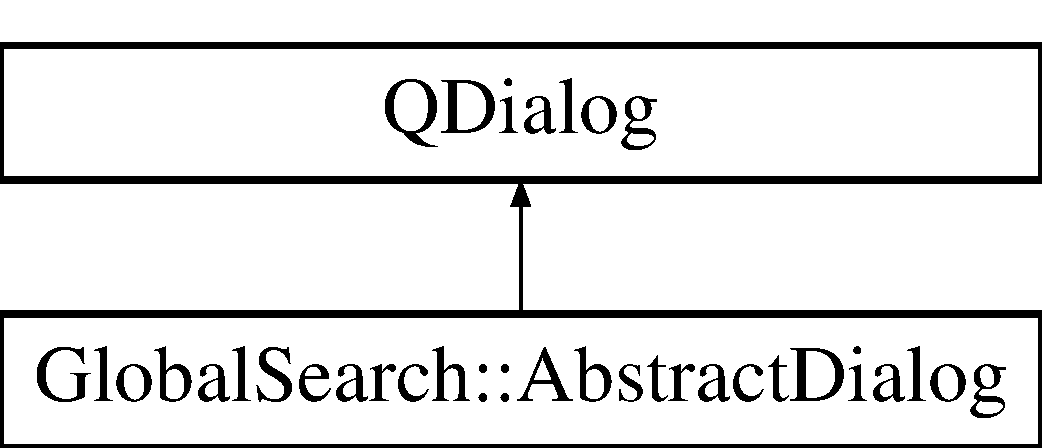
\includegraphics[height=2.000000cm]{classGlobalSearch_1_1AbstractDialog}
\end{center}
\end{figure}
\subsubsection*{Public Slots}
\begin{DoxyCompactItemize}
\item 
virtual void \hyperlink{classGlobalSearch_1_1AbstractDialog_af25e016b17402f6695eb9428c197bce6}{disconnect\+G\+U\+I} ()
\item 
virtual void \hyperlink{classGlobalSearch_1_1AbstractDialog_af0a84714b098c38a3311299fc7f547bc}{lock\+G\+U\+I} ()
\item 
virtual void \hyperlink{classGlobalSearch_1_1AbstractDialog_a70a82283ccccb007cf0142f2e166240f}{update\+G\+U\+I} ()
\item 
virtual void \hyperlink{classGlobalSearch_1_1AbstractDialog_afab2e36367be4fa97e891b020afd1e60}{write\+Settings} (const Q\+String \&filename=\char`\"{}\char`\"{})
\end{DoxyCompactItemize}
\subsubsection*{Signals}
\begin{DoxyCompactItemize}
\item 
void \hyperlink{classGlobalSearch_1_1AbstractDialog_a3557cb9d441d0aabbd9ee3aa8cfdaea9}{tabs\+Disconnect\+G\+U\+I} ()
\item 
void \hyperlink{classGlobalSearch_1_1AbstractDialog_a93ef632734bcb7228216f5685e90e3f1}{tabs\+Lock\+G\+U\+I} ()
\item 
void \hyperlink{classGlobalSearch_1_1AbstractDialog_a17e7f95159cbbf74b44739636271bc59}{tabs\+Write\+Settings} (const Q\+String \&filename)
\item 
void \hyperlink{classGlobalSearch_1_1AbstractDialog_aac4850039323bd7bf05f048bc7e8437e}{tabs\+Read\+Settings} (const Q\+String \&filename)
\item 
void \hyperlink{classGlobalSearch_1_1AbstractDialog_aea96d15a1dcd0715e4cd2b4377f052d0}{tabs\+Update\+G\+U\+I} ()
\item 
void \hyperlink{classGlobalSearch_1_1AbstractDialog_ac9ca934578ad9620bf49b9074a2b6982}{molecule\+Changed} (\hyperlink{classGlobalSearch_1_1Structure}{Global\+Search\+::\+Structure} $\ast$)
\item 
void \hyperlink{classGlobalSearch_1_1AbstractDialog_a94fdb4c5a3ec5963f2764f0d821b2583}{new\+Log} (const Q\+String \&str)
\item 
void \hyperlink{classGlobalSearch_1_1AbstractDialog_a99f0d05314c6da0ceb54cac2fd911c00}{sig\+\_\+update\+Status} (int, int, int)
\item 
void \hyperlink{classGlobalSearch_1_1AbstractDialog_a85a70ecb4d340cfeae15c18f69419827}{sig\+\_\+start\+Progress\+Update} (const Q\+String \&, int, int)
\item 
void \hyperlink{classGlobalSearch_1_1AbstractDialog_a738c3769545f233bb38b45a4724d527d}{sig\+\_\+stop\+Progress\+Update} ()
\item 
void \hyperlink{classGlobalSearch_1_1AbstractDialog_ab4aa18927ac8220ed98cdd6367eb1416}{sig\+\_\+update\+Progress\+Minimum} (int)
\item 
void \hyperlink{classGlobalSearch_1_1AbstractDialog_a8eb81a20fe5ad425482d3400d868fa16}{sig\+\_\+update\+Progress\+Maximum} (int)
\item 
void \hyperlink{classGlobalSearch_1_1AbstractDialog_adac485f7c7d5ac013a12b183a814da95}{sig\+\_\+update\+Progress\+Value} (int)
\item 
void \hyperlink{classGlobalSearch_1_1AbstractDialog_a4201bb13ca8322d5031ad7065d9f4afd}{sig\+\_\+update\+Progress\+Label} (const Q\+String \&)
\item 
void \hyperlink{classGlobalSearch_1_1AbstractDialog_a171b7b488362e506ba05e1016d3de0b0}{sig\+\_\+repaint\+Progress\+Bar} ()
\item 
void \hyperlink{classGlobalSearch_1_1AbstractDialog_a3d14409c0c74cea8b4b3e32e3a9eb7d0}{sig\+\_\+error\+Box} (const Q\+String \&)
\end{DoxyCompactItemize}
\subsubsection*{Public Member Functions}
\begin{DoxyCompactItemize}
\item 
\hyperlink{classGlobalSearch_1_1AbstractDialog_a44af0af55038d330e284d3ddc567dd3f}{Abstract\+Dialog} (Avogadro\+::\+G\+L\+Widget $\ast$gl\+Widget=0, Q\+Widget $\ast$parent=0, Qt\+::\+Window\+Flags f=0)
\item 
void \hyperlink{classGlobalSearch_1_1AbstractDialog_aea19edd77198f2e6155002f53a61add6}{initialize} ()
\item 
virtual \hyperlink{classGlobalSearch_1_1AbstractDialog_a55ebf148332cc0eca585e816bda871ae}{$\sim$\+Abstract\+Dialog} ()
\item 
Avogadro\+::\+G\+L\+Widget $\ast$ \hyperlink{classGlobalSearch_1_1AbstractDialog_a4823851b13319cd2a4384c00346faf22}{get\+G\+L\+Widget} ()
\item 
\hyperlink{classGlobalSearch_1_1OptBase}{Opt\+Base} $\ast$ \hyperlink{classGlobalSearch_1_1AbstractDialog_ad2fe5c3c110152b29207b54df72dbd45}{get\+Opt\+Base} ()
\item 
virtual void \hyperlink{classGlobalSearch_1_1AbstractDialog_aa798b5d3d1099bce37207a3f15b0eb6a}{read\+Settings} (const Q\+String \&filename=\char`\"{}\char`\"{})
\item 
virtual void \hyperlink{classGlobalSearch_1_1AbstractDialog_a6e9ef21da0b2e60513a11f7de55ffbd7}{save\+Session} ()=0
\item 
void \hyperlink{classGlobalSearch_1_1AbstractDialog_a40bbc9eb104fe418e1fb2ba93bd2a2ae}{update\+Status} (int opt, int run, int fail)
\item 
void \hyperlink{classGlobalSearch_1_1AbstractDialog_a861a8ddbb5ca235f5966737755911aa3}{set\+G\+L\+Widget} (Avogadro\+::\+G\+L\+Widget $\ast$w)
\item 
void \hyperlink{classGlobalSearch_1_1AbstractDialog_a7353bd5b3393faf017287674691e56c6}{new\+Debug} (const Q\+String \&s)
\item 
void \hyperlink{classGlobalSearch_1_1AbstractDialog_abe3084783126e2d1f09c9250c11f8f39}{new\+Warning} (const Q\+String \&s)
\item 
void \hyperlink{classGlobalSearch_1_1AbstractDialog_ae0b664aa133ded37df0dc5f7a040f0c5}{new\+Error} (const Q\+String \&s)
\item 
void \hyperlink{classGlobalSearch_1_1AbstractDialog_aee94863a2a275b8a91613b191451bc1e}{error\+Box} (const Q\+String \&s)
\end{DoxyCompactItemize}
\begin{Indent}{\bf Progressbar functions}\par
{\em These functions are used to display and control a progress notification system for log processes. }\begin{DoxyCompactItemize}
\item 
void \hyperlink{classGlobalSearch_1_1AbstractDialog_ac2b3d31770c83a49b8d817a857ef377e}{start\+Progress\+Update} (const Q\+String \&text, int min, int max)
\item 
void \hyperlink{classGlobalSearch_1_1AbstractDialog_a5159109a62a0d755a6d201bce5ab6466}{stop\+Progress\+Update} ()
\item 
void \hyperlink{classGlobalSearch_1_1AbstractDialog_a37d58a75a23e7082963937caba89e47f}{update\+Progress\+Minimum} (int min)
\item 
void \hyperlink{classGlobalSearch_1_1AbstractDialog_aeadfeb3807fd25918136263e13634827}{update\+Progress\+Maximum} (int max)
\item 
void \hyperlink{classGlobalSearch_1_1AbstractDialog_a33bc475a9faf3f8307beaa2b20bf3c1c}{update\+Progress\+Value} (int val)
\item 
void \hyperlink{classGlobalSearch_1_1AbstractDialog_a74180c40bc787fae62909aa3cde450a3}{update\+Progress\+Label} (const Q\+String \&text)
\item 
void \hyperlink{classGlobalSearch_1_1AbstractDialog_a2b2e126bf000fb92e962f1c4db71a231}{repaint\+Progress\+Bar} ()
\end{DoxyCompactItemize}
\end{Indent}
\subsubsection*{Protected Slots}
\begin{DoxyCompactItemize}
\item 
virtual void \hyperlink{classGlobalSearch_1_1AbstractDialog_a40b7d250a73097f76edb2d77fce5482e}{start\+Search} ()=0
\item 
virtual void \hyperlink{classGlobalSearch_1_1AbstractDialog_a503a264e1a67559ace47d15d2c3aa61b}{resume\+Session} ()
\item 
void \hyperlink{classGlobalSearch_1_1AbstractDialog_ae5276198173f5a0da4a64adedc46f676}{update\+Status\+\_\+} (int, int, int)
\item 
void \hyperlink{classGlobalSearch_1_1AbstractDialog_a5370d90758c991200a233a78a1a51d16}{start\+Progress\+Update\+\_\+} (const Q\+String \&, int, int)
\item 
void \hyperlink{classGlobalSearch_1_1AbstractDialog_a5dd0aa68a9c1445965b9900290d4a507}{stop\+Progress\+Update\+\_\+} ()
\item 
void \hyperlink{classGlobalSearch_1_1AbstractDialog_a9013ffdb7bcec2ce4e6fec13fb0f1c0a}{update\+Progress\+Minimum\+\_\+} (int)
\item 
void \hyperlink{classGlobalSearch_1_1AbstractDialog_aa346e6c775c7edc9e423134ef8842c7b}{update\+Progress\+Maximum\+\_\+} (int)
\item 
void \hyperlink{classGlobalSearch_1_1AbstractDialog_af4c90078d59537ef9b9f7d69cbdc09c2}{update\+Progress\+Value\+\_\+} (int)
\item 
void \hyperlink{classGlobalSearch_1_1AbstractDialog_aff9811ebc7606ac13ae33b6130697fa9}{update\+Progress\+Label\+\_\+} (const Q\+String \&)
\item 
void \hyperlink{classGlobalSearch_1_1AbstractDialog_a455ad76e725fe59cd6f260d2c90d7a6d}{repaint\+Progress\+Bar\+\_\+} ()
\item 
void \hyperlink{classGlobalSearch_1_1AbstractDialog_a4ccf7b6a73663c780f82c2c6f4a39536}{error\+Box\+\_\+} (const Q\+String \&s)
\end{DoxyCompactItemize}
\subsubsection*{Protected Member Functions}
\begin{DoxyCompactItemize}
\item 
virtual void \hyperlink{classGlobalSearch_1_1AbstractDialog_a4ef7df380968131422757b20889d37b0}{resume\+Session\+\_\+} (const Q\+String \&filename)
\end{DoxyCompactItemize}
\subsubsection*{Protected Attributes}
\begin{DoxyCompactItemize}
\item 
\hyperlink{classGlobalSearch_1_1OptBase}{Opt\+Base} $\ast$ \hyperlink{classGlobalSearch_1_1AbstractDialog_a6a5b08f59d1521ebc4769e9e9903346b}{m\+\_\+opt}
\item 
Avogadro\+::\+Molecule $\ast$ \hyperlink{classGlobalSearch_1_1AbstractDialog_a9cf65fe592eebca0ec72a5597edc7faf}{m\+\_\+molecule}
\item 
Avogadro\+::\+G\+L\+Widget $\ast$ \hyperlink{classGlobalSearch_1_1AbstractDialog_a18c6963416c0b49012fa94fd451c96d9}{m\+\_\+gl\+Widget}
\item 
Q\+Mutex $\ast$ \hyperlink{classGlobalSearch_1_1AbstractDialog_a06e3b73c319208a706aaf629a5f05165}{prog\+Mutex}
\item 
Q\+Timer $\ast$ \hyperlink{classGlobalSearch_1_1AbstractDialog_a1cf317e8206fd80628a9fe6d2ec711fc}{prog\+Timer}
\item 
Q\+Push\+Button $\ast$ \hyperlink{classGlobalSearch_1_1AbstractDialog_a526c9ad4ea52454ba41be74de24cdd6c}{ui\+\_\+push\+\_\+begin}
\item 
Q\+Push\+Button $\ast$ \hyperlink{classGlobalSearch_1_1AbstractDialog_a695ed25af57ce8c854e21d3f2c18e250}{ui\+\_\+push\+\_\+save}
\item 
Q\+Push\+Button $\ast$ \hyperlink{classGlobalSearch_1_1AbstractDialog_a04a1131601c5eab39ef105f385aceca5}{ui\+\_\+push\+\_\+resume}
\item 
Q\+Label $\ast$ \hyperlink{classGlobalSearch_1_1AbstractDialog_af30548b5ed4d5a22a7dc648afae4115b}{ui\+\_\+label\+\_\+opt}
\item 
Q\+Label $\ast$ \hyperlink{classGlobalSearch_1_1AbstractDialog_af65c818f2bf846bcd76aa0e755e13453}{ui\+\_\+label\+\_\+run}
\item 
Q\+Label $\ast$ \hyperlink{classGlobalSearch_1_1AbstractDialog_a28b127a410ed219e13a0e85c889934e7}{ui\+\_\+label\+\_\+fail}
\item 
Q\+Label $\ast$ \hyperlink{classGlobalSearch_1_1AbstractDialog_a21e1395aea6ac29a9c97b7ec2f54eb14}{ui\+\_\+label\+\_\+prog}
\item 
Q\+Progress\+Bar $\ast$ \hyperlink{classGlobalSearch_1_1AbstractDialog_a9b91400d03e9c7f3e94bf6b1f91bb97a}{ui\+\_\+progbar}
\item 
Q\+Tab\+Widget $\ast$ \hyperlink{classGlobalSearch_1_1AbstractDialog_acc93d22a99eb7c11610494ce754b1502}{ui\+\_\+tabs}
\end{DoxyCompactItemize}


\subsubsection{Detailed Description}
A basic dialog that is preconfigured for use with Global\+Search. 

\begin{DoxyAuthor}{Author}
David C. Lonie
\end{DoxyAuthor}
\hyperlink{classGlobalSearch_1_1AbstractDialog}{Abstract\+Dialog} is set up for use with an \hyperlink{classGlobalSearch_1_1OptBase}{Opt\+Base} class. See the accompanying .ui file for a Qt\+Designer template.

To properly use this class, modify abstractdialog.\+ui in Qt Designer without changing the names of any existing elements. Do not add tabs, this will be done later programmatically.

Include a block like this in the derived class\textquotesingle{}s constructor to setup the U\+I\+: \begin{DoxyVerb}    // Initialize UI
    ui.setupUi(this);
    ui_push_begin   = ui.push_begin;
    ui_push_save    = ui.push_save;
    ui_push_resume  = ui.push_resume;
    ui_label_opt    = ui.label_opt;
    ui_label_run    = ui.label_run;
    ui_label_fail   = ui.label_fail;
    ui_label_prog   = ui.label_prog;
    ui_progbar      = ui.progbar;
    ui_tabs         = ui.tabs;

    // Tabs: be sure to include and define in derived header.
    // Initialize tabs (modify as needed)
    m_tab_init     = new TabInit(this, m_opt);
    m_tab_edit     = new TabEdit(this, m_opt);
    m_tab_opt      = new TabOpt(this, m_opt);
    m_tab_sys      = new TabSys(this, m_opt);
    m_tab_progress = new TabProgress(this, m_opt);
    m_tab_plot     = new TabPlot(this, m_opt);
    m_tab_log      = new TabLog(this, m_opt);

    // Populate tab widget (modify as needed)
    ui.tabs->clear();
    ui.tabs->addTab(m_tab_init->getTabWidget(),     tr("Cell &Initialization"));
    ui.tabs->addTab(m_tab_edit->getTabWidget(),     tr("Optimization &Templates"));
    ui.tabs->addTab(m_tab_opt->getTabWidget(),      tr("&Optimization Settings"));
    ui.tabs->addTab(m_tab_sys->getTabWidget(),      tr("&System Settings"));
    ui.tabs->addTab(m_tab_progress->getTabWidget(), tr("&Progress"));
    ui.tabs->addTab(m_tab_plot->getTabWidget(),     tr("&Plot"));
    ui.tabs->addTab(m_tab_log->getTabWidget(),      tr("&Log"));

    // Select the first tab by default
    ui.tabs->setCurrentIndex(0);

    // Hide the progress bar/label
    ui.label_prog->setVisible(false);
    ui.progbar->setVisible(false);
\end{DoxyVerb}
 \begin{DoxyVerb} It is also essential to call initialize() at the end of the
 derived constructor.\end{DoxyVerb}
 

Definition at line 99 of file abstractdialog.\+h.



\subsubsection{Constructor \& Destructor Documentation}
\hypertarget{classGlobalSearch_1_1AbstractDialog_a44af0af55038d330e284d3ddc567dd3f}{}\index{Global\+Search\+::\+Abstract\+Dialog@{Global\+Search\+::\+Abstract\+Dialog}!Abstract\+Dialog@{Abstract\+Dialog}}
\index{Abstract\+Dialog@{Abstract\+Dialog}!Global\+Search\+::\+Abstract\+Dialog@{Global\+Search\+::\+Abstract\+Dialog}}
\paragraph[{Abstract\+Dialog}]{\setlength{\rightskip}{0pt plus 5cm}Global\+Search\+::\+Abstract\+Dialog\+::\+Abstract\+Dialog (
\begin{DoxyParamCaption}
\item[{Avogadro\+::\+G\+L\+Widget $\ast$}]{gl\+Widget = {\ttfamily 0}, }
\item[{Q\+Widget $\ast$}]{parent = {\ttfamily 0}, }
\item[{Qt\+::\+Window\+Flags}]{f = {\ttfamily 0}}
\end{DoxyParamCaption}
)\hspace{0.3cm}{\ttfamily [explicit]}}\label{classGlobalSearch_1_1AbstractDialog_a44af0af55038d330e284d3ddc567dd3f}
Constructor.

When deriving, be sure to call \hyperlink{classGlobalSearch_1_1AbstractDialog_aea19edd77198f2e6155002f53a61add6}{initialize()} after initializing m\+\_\+opt and ui. \begin{DoxySeeAlso}{See also}
\hyperlink{classGlobalSearch_1_1AbstractDialog_aea19edd77198f2e6155002f53a61add6}{initialize} 
\end{DoxySeeAlso}

\begin{DoxyParams}{Parameters}
{\em gl\+Widget} & The G\+Lwidget from the Avogadro instance \\
\hline
{\em parent} & Parent object \\
\hline
{\em f} & Window flags \\
\hline
\end{DoxyParams}


Definition at line 39 of file abstractdialog.\+cpp.



References prog\+Mutex, and prog\+Timer.

\hypertarget{classGlobalSearch_1_1AbstractDialog_a55ebf148332cc0eca585e816bda871ae}{}\index{Global\+Search\+::\+Abstract\+Dialog@{Global\+Search\+::\+Abstract\+Dialog}!````~Abstract\+Dialog@{$\sim$\+Abstract\+Dialog}}
\index{````~Abstract\+Dialog@{$\sim$\+Abstract\+Dialog}!Global\+Search\+::\+Abstract\+Dialog@{Global\+Search\+::\+Abstract\+Dialog}}
\paragraph[{$\sim$\+Abstract\+Dialog}]{\setlength{\rightskip}{0pt plus 5cm}Global\+Search\+::\+Abstract\+Dialog\+::$\sim$\+Abstract\+Dialog (
\begin{DoxyParamCaption}
{}
\end{DoxyParamCaption}
)\hspace{0.3cm}{\ttfamily [virtual]}}\label{classGlobalSearch_1_1AbstractDialog_a55ebf148332cc0eca585e816bda871ae}
Destructor. Deletes m\+\_\+opt.

Consider calling something along the lines of \begin{DoxyVerb}    if (m_opt->saveOnExit) {
      m_opt->tracker()->lockForRead();
      writeSettings();
      saveSession();
      m_opt->tracker()->unlock();
    }
\end{DoxyVerb}
 in the derived destructor. 

Definition at line 140 of file abstractdialog.\+cpp.



References m\+\_\+opt.



\subsubsection{Member Function Documentation}
\hypertarget{classGlobalSearch_1_1AbstractDialog_af25e016b17402f6695eb9428c197bce6}{}\index{Global\+Search\+::\+Abstract\+Dialog@{Global\+Search\+::\+Abstract\+Dialog}!disconnect\+G\+U\+I@{disconnect\+G\+U\+I}}
\index{disconnect\+G\+U\+I@{disconnect\+G\+U\+I}!Global\+Search\+::\+Abstract\+Dialog@{Global\+Search\+::\+Abstract\+Dialog}}
\paragraph[{disconnect\+G\+U\+I}]{\setlength{\rightskip}{0pt plus 5cm}void Global\+Search\+::\+Abstract\+Dialog\+::disconnect\+G\+U\+I (
\begin{DoxyParamCaption}
{}
\end{DoxyParamCaption}
)\hspace{0.3cm}{\ttfamily [virtual]}, {\ttfamily [slot]}}\label{classGlobalSearch_1_1AbstractDialog_af25e016b17402f6695eb9428c197bce6}
Call this to disable G\+U\+I updates. Useful when benchmarking non-\/interactively. \begin{DoxyNote}{Note}
This call is passed on to all tabs. 
\end{DoxyNote}


Definition at line 145 of file abstractdialog.\+cpp.



References m\+\_\+opt, sig\+\_\+update\+Status(), tabs\+Disconnect\+G\+U\+I(), update\+G\+U\+I(), and update\+Status\+\_\+().

\hypertarget{classGlobalSearch_1_1AbstractDialog_aee94863a2a275b8a91613b191451bc1e}{}\index{Global\+Search\+::\+Abstract\+Dialog@{Global\+Search\+::\+Abstract\+Dialog}!error\+Box@{error\+Box}}
\index{error\+Box@{error\+Box}!Global\+Search\+::\+Abstract\+Dialog@{Global\+Search\+::\+Abstract\+Dialog}}
\paragraph[{error\+Box}]{\setlength{\rightskip}{0pt plus 5cm}void Global\+Search\+::\+Abstract\+Dialog\+::error\+Box (
\begin{DoxyParamCaption}
\item[{const Q\+String \&}]{s}
\end{DoxyParamCaption}
)\hspace{0.3cm}{\ttfamily [inline]}}\label{classGlobalSearch_1_1AbstractDialog_aee94863a2a275b8a91613b191451bc1e}
Displays an error box with the indicated message. This function will block the G\+U\+I thread until user clicks \char`\"{}\+Ok\char`\"{}.

\begin{DoxyNote}{Note}
Do not use this function, but instead send call \hyperlink{classGlobalSearch_1_1OptBase_a0069abbd35393e6a5760b049e3497a21}{Opt\+Base\+::error}
\end{DoxyNote}

\begin{DoxyParams}{Parameters}
{\em s} & Error message. \\
\hline
\end{DoxyParams}


Definition at line 335 of file abstractdialog.\+h.



References sig\+\_\+error\+Box().



Referenced by new\+Error().

\hypertarget{classGlobalSearch_1_1AbstractDialog_a4ccf7b6a73663c780f82c2c6f4a39536}{}\index{Global\+Search\+::\+Abstract\+Dialog@{Global\+Search\+::\+Abstract\+Dialog}!error\+Box\+\_\+@{error\+Box\+\_\+}}
\index{error\+Box\+\_\+@{error\+Box\+\_\+}!Global\+Search\+::\+Abstract\+Dialog@{Global\+Search\+::\+Abstract\+Dialog}}
\paragraph[{error\+Box\+\_\+}]{\setlength{\rightskip}{0pt plus 5cm}void Global\+Search\+::\+Abstract\+Dialog\+::error\+Box\+\_\+ (
\begin{DoxyParamCaption}
\item[{const Q\+String \&}]{s}
\end{DoxyParamCaption}
)\hspace{0.3cm}{\ttfamily [inline]}, {\ttfamily [protected]}, {\ttfamily [slot]}}\label{classGlobalSearch_1_1AbstractDialog_a4ccf7b6a73663c780f82c2c6f4a39536}
Hidden call. Ensures that the G\+U\+I is modified from the appropriate thread. \begin{DoxySeeAlso}{See also}
\hyperlink{classGlobalSearch_1_1AbstractDialog_aee94863a2a275b8a91613b191451bc1e}{error\+Box} 
\end{DoxySeeAlso}


Definition at line 415 of file abstractdialog.\+h.



Referenced by initialize().

\hypertarget{classGlobalSearch_1_1AbstractDialog_a4823851b13319cd2a4384c00346faf22}{}\index{Global\+Search\+::\+Abstract\+Dialog@{Global\+Search\+::\+Abstract\+Dialog}!get\+G\+L\+Widget@{get\+G\+L\+Widget}}
\index{get\+G\+L\+Widget@{get\+G\+L\+Widget}!Global\+Search\+::\+Abstract\+Dialog@{Global\+Search\+::\+Abstract\+Dialog}}
\paragraph[{get\+G\+L\+Widget}]{\setlength{\rightskip}{0pt plus 5cm}Avogadro\+::\+G\+L\+Widget$\ast$ Global\+Search\+::\+Abstract\+Dialog\+::get\+G\+L\+Widget (
\begin{DoxyParamCaption}
{}
\end{DoxyParamCaption}
)\hspace{0.3cm}{\ttfamily [inline]}}\label{classGlobalSearch_1_1AbstractDialog_a4823851b13319cd2a4384c00346faf22}
\begin{DoxyReturn}{Returns}
The G\+L\+Widget of the main Avogadro window. 
\end{DoxyReturn}


Definition at line 144 of file abstractdialog.\+h.



References m\+\_\+gl\+Widget.

\hypertarget{classGlobalSearch_1_1AbstractDialog_ad2fe5c3c110152b29207b54df72dbd45}{}\index{Global\+Search\+::\+Abstract\+Dialog@{Global\+Search\+::\+Abstract\+Dialog}!get\+Opt\+Base@{get\+Opt\+Base}}
\index{get\+Opt\+Base@{get\+Opt\+Base}!Global\+Search\+::\+Abstract\+Dialog@{Global\+Search\+::\+Abstract\+Dialog}}
\paragraph[{get\+Opt\+Base}]{\setlength{\rightskip}{0pt plus 5cm}{\bf Opt\+Base}$\ast$ Global\+Search\+::\+Abstract\+Dialog\+::get\+Opt\+Base (
\begin{DoxyParamCaption}
{}
\end{DoxyParamCaption}
)\hspace{0.3cm}{\ttfamily [inline]}}\label{classGlobalSearch_1_1AbstractDialog_ad2fe5c3c110152b29207b54df72dbd45}
\begin{DoxyReturn}{Returns}
The associated \hyperlink{classGlobalSearch_1_1OptBase}{Opt\+Base} derived class. 
\end{DoxyReturn}


Definition at line 149 of file abstractdialog.\+h.



References m\+\_\+opt.

\hypertarget{classGlobalSearch_1_1AbstractDialog_aea19edd77198f2e6155002f53a61add6}{}\index{Global\+Search\+::\+Abstract\+Dialog@{Global\+Search\+::\+Abstract\+Dialog}!initialize@{initialize}}
\index{initialize@{initialize}!Global\+Search\+::\+Abstract\+Dialog@{Global\+Search\+::\+Abstract\+Dialog}}
\paragraph[{initialize}]{\setlength{\rightskip}{0pt plus 5cm}void Global\+Search\+::\+Abstract\+Dialog\+::initialize (
\begin{DoxyParamCaption}
{}
\end{DoxyParamCaption}
)}\label{classGlobalSearch_1_1AbstractDialog_aea19edd77198f2e6155002f53a61add6}
Connect m\+\_\+opt and the ui to the dialog. Call this in the derived class\textquotesingle{}s constructor after initializing m\+\_\+opt and the private ui\+\_\+$\ast$ member variables. 

Definition at line 55 of file abstractdialog.\+cpp.



References error\+Box\+\_\+(), lock\+G\+U\+I(), m\+\_\+opt, new\+Debug(), new\+Error(), new\+Warning(), prog\+Timer, Global\+Search\+::\+Opt\+Base\+::queue(), read\+Settings(), repaint\+Progress\+Bar\+\_\+(), resume\+Session(), save\+Session(), sig\+\_\+error\+Box(), sig\+\_\+repaint\+Progress\+Bar(), sig\+\_\+start\+Progress\+Update(), sig\+\_\+stop\+Progress\+Update(), sig\+\_\+update\+Progress\+Label(), sig\+\_\+update\+Progress\+Maximum(), sig\+\_\+update\+Progress\+Minimum(), sig\+\_\+update\+Progress\+Value(), sig\+\_\+update\+Status(), start\+Progress\+Update\+\_\+(), start\+Search(), stop\+Progress\+Update\+\_\+(), tabs\+Read\+Settings(), tabs\+Write\+Settings(), Global\+Search\+::\+Opt\+Base\+::tracker(), ui\+\_\+label\+\_\+prog, ui\+\_\+progbar, ui\+\_\+push\+\_\+begin, ui\+\_\+push\+\_\+resume, ui\+\_\+push\+\_\+save, ui\+\_\+tabs, update\+G\+U\+I(), update\+Progress\+Label\+\_\+(), update\+Progress\+Maximum\+\_\+(), update\+Progress\+Minimum\+\_\+(), update\+Progress\+Value\+\_\+(), update\+Status(), and update\+Status\+\_\+().

\hypertarget{classGlobalSearch_1_1AbstractDialog_af0a84714b098c38a3311299fc7f547bc}{}\index{Global\+Search\+::\+Abstract\+Dialog@{Global\+Search\+::\+Abstract\+Dialog}!lock\+G\+U\+I@{lock\+G\+U\+I}}
\index{lock\+G\+U\+I@{lock\+G\+U\+I}!Global\+Search\+::\+Abstract\+Dialog@{Global\+Search\+::\+Abstract\+Dialog}}
\paragraph[{lock\+G\+U\+I}]{\setlength{\rightskip}{0pt plus 5cm}void Global\+Search\+::\+Abstract\+Dialog\+::lock\+G\+U\+I (
\begin{DoxyParamCaption}
{}
\end{DoxyParamCaption}
)\hspace{0.3cm}{\ttfamily [virtual]}, {\ttfamily [slot]}}\label{classGlobalSearch_1_1AbstractDialog_af0a84714b098c38a3311299fc7f547bc}
Called when the search session starts to disable G\+U\+I components that should only be modified during initialization. \begin{DoxyNote}{Note}
This call is passed on to all tabs. 
\end{DoxyNote}


Definition at line 155 of file abstractdialog.\+cpp.



References tabs\+Lock\+G\+U\+I(), ui\+\_\+push\+\_\+begin, ui\+\_\+push\+\_\+resume, and ui\+\_\+push\+\_\+save.



Referenced by initialize().

\hypertarget{classGlobalSearch_1_1AbstractDialog_ac9ca934578ad9620bf49b9074a2b6982}{}\index{Global\+Search\+::\+Abstract\+Dialog@{Global\+Search\+::\+Abstract\+Dialog}!molecule\+Changed@{molecule\+Changed}}
\index{molecule\+Changed@{molecule\+Changed}!Global\+Search\+::\+Abstract\+Dialog@{Global\+Search\+::\+Abstract\+Dialog}}
\paragraph[{molecule\+Changed}]{\setlength{\rightskip}{0pt plus 5cm}void Global\+Search\+::\+Abstract\+Dialog\+::molecule\+Changed (
\begin{DoxyParamCaption}
\item[{{\bf Global\+Search\+::\+Structure} $\ast$}]{}
\end{DoxyParamCaption}
)\hspace{0.3cm}{\ttfamily [signal]}}\label{classGlobalSearch_1_1AbstractDialog_ac9ca934578ad9620bf49b9074a2b6982}
Emitted to change/update the molecule displayed in the Avogadro main window. \hypertarget{classGlobalSearch_1_1AbstractDialog_a7353bd5b3393faf017287674691e56c6}{}\index{Global\+Search\+::\+Abstract\+Dialog@{Global\+Search\+::\+Abstract\+Dialog}!new\+Debug@{new\+Debug}}
\index{new\+Debug@{new\+Debug}!Global\+Search\+::\+Abstract\+Dialog@{Global\+Search\+::\+Abstract\+Dialog}}
\paragraph[{new\+Debug}]{\setlength{\rightskip}{0pt plus 5cm}void Global\+Search\+::\+Abstract\+Dialog\+::new\+Debug (
\begin{DoxyParamCaption}
\item[{const Q\+String \&}]{s}
\end{DoxyParamCaption}
)\hspace{0.3cm}{\ttfamily [inline]}}\label{classGlobalSearch_1_1AbstractDialog_a7353bd5b3393faf017287674691e56c6}
Called by \hyperlink{classGlobalSearch_1_1OptBase_a3e24cda71c456027edbcab36c9a5e08c}{Opt\+Base\+::debug} and sends a message to the log tab.

\begin{DoxyNote}{Note}
Do not use this function, but instead send call \hyperlink{classGlobalSearch_1_1OptBase_a3e24cda71c456027edbcab36c9a5e08c}{Opt\+Base\+::debug}
\end{DoxyNote}

\begin{DoxyParams}{Parameters}
{\em s} & The debugging message. \\
\hline
\end{DoxyParams}


Definition at line 302 of file abstractdialog.\+h.



References new\+Log().



Referenced by initialize().

\hypertarget{classGlobalSearch_1_1AbstractDialog_ae0b664aa133ded37df0dc5f7a040f0c5}{}\index{Global\+Search\+::\+Abstract\+Dialog@{Global\+Search\+::\+Abstract\+Dialog}!new\+Error@{new\+Error}}
\index{new\+Error@{new\+Error}!Global\+Search\+::\+Abstract\+Dialog@{Global\+Search\+::\+Abstract\+Dialog}}
\paragraph[{new\+Error}]{\setlength{\rightskip}{0pt plus 5cm}void Global\+Search\+::\+Abstract\+Dialog\+::new\+Error (
\begin{DoxyParamCaption}
\item[{const Q\+String \&}]{s}
\end{DoxyParamCaption}
)\hspace{0.3cm}{\ttfamily [inline]}}\label{classGlobalSearch_1_1AbstractDialog_ae0b664aa133ded37df0dc5f7a040f0c5}
Called by \hyperlink{classGlobalSearch_1_1OptBase_a0069abbd35393e6a5760b049e3497a21}{Opt\+Base\+::error}. Sends a message to the log tab and calls error\+Box.

\begin{DoxyNote}{Note}
Do not use this function, but instead send call \hyperlink{classGlobalSearch_1_1OptBase_a0069abbd35393e6a5760b049e3497a21}{Opt\+Base\+::error}
\end{DoxyNote}

\begin{DoxyParams}{Parameters}
{\em s} & The error message. \\
\hline
\end{DoxyParams}


Definition at line 323 of file abstractdialog.\+h.



References error\+Box(), and new\+Log().



Referenced by initialize().

\hypertarget{classGlobalSearch_1_1AbstractDialog_a94fdb4c5a3ec5963f2764f0d821b2583}{}\index{Global\+Search\+::\+Abstract\+Dialog@{Global\+Search\+::\+Abstract\+Dialog}!new\+Log@{new\+Log}}
\index{new\+Log@{new\+Log}!Global\+Search\+::\+Abstract\+Dialog@{Global\+Search\+::\+Abstract\+Dialog}}
\paragraph[{new\+Log}]{\setlength{\rightskip}{0pt plus 5cm}void Global\+Search\+::\+Abstract\+Dialog\+::new\+Log (
\begin{DoxyParamCaption}
\item[{const Q\+String \&}]{str}
\end{DoxyParamCaption}
)\hspace{0.3cm}{\ttfamily [signal]}}\label{classGlobalSearch_1_1AbstractDialog_a94fdb4c5a3ec5963f2764f0d821b2583}
Emitted when there is a new log message ready. \begin{DoxySeeAlso}{See also}
\hyperlink{classGlobalSearch_1_1OptBase_a3e24cda71c456027edbcab36c9a5e08c}{Opt\+Base\+::debug} 

\hyperlink{classGlobalSearch_1_1OptBase_a4f70a04b72a92665b7fb6f8e868b527e}{Opt\+Base\+::warning} 

\hyperlink{classGlobalSearch_1_1OptBase_a0069abbd35393e6a5760b049e3497a21}{Opt\+Base\+::error} 
\end{DoxySeeAlso}

\begin{DoxyParams}{Parameters}
{\em str} & Log message \\
\hline
\end{DoxyParams}


Referenced by new\+Debug(), new\+Error(), and new\+Warning().

\hypertarget{classGlobalSearch_1_1AbstractDialog_abe3084783126e2d1f09c9250c11f8f39}{}\index{Global\+Search\+::\+Abstract\+Dialog@{Global\+Search\+::\+Abstract\+Dialog}!new\+Warning@{new\+Warning}}
\index{new\+Warning@{new\+Warning}!Global\+Search\+::\+Abstract\+Dialog@{Global\+Search\+::\+Abstract\+Dialog}}
\paragraph[{new\+Warning}]{\setlength{\rightskip}{0pt plus 5cm}void Global\+Search\+::\+Abstract\+Dialog\+::new\+Warning (
\begin{DoxyParamCaption}
\item[{const Q\+String \&}]{s}
\end{DoxyParamCaption}
)\hspace{0.3cm}{\ttfamily [inline]}}\label{classGlobalSearch_1_1AbstractDialog_abe3084783126e2d1f09c9250c11f8f39}
Called by \hyperlink{classGlobalSearch_1_1OptBase_a4f70a04b72a92665b7fb6f8e868b527e}{Opt\+Base\+::warning} and sends a message to the log tab.

\begin{DoxyNote}{Note}
Do not use this function, but instead send call \hyperlink{classGlobalSearch_1_1OptBase_a4f70a04b72a92665b7fb6f8e868b527e}{Opt\+Base\+::warning}
\end{DoxyNote}

\begin{DoxyParams}{Parameters}
{\em s} & The warning message. \\
\hline
\end{DoxyParams}


Definition at line 312 of file abstractdialog.\+h.



References new\+Log().



Referenced by initialize().

\hypertarget{classGlobalSearch_1_1AbstractDialog_aa798b5d3d1099bce37207a3f15b0eb6a}{}\index{Global\+Search\+::\+Abstract\+Dialog@{Global\+Search\+::\+Abstract\+Dialog}!read\+Settings@{read\+Settings}}
\index{read\+Settings@{read\+Settings}!Global\+Search\+::\+Abstract\+Dialog@{Global\+Search\+::\+Abstract\+Dialog}}
\paragraph[{read\+Settings}]{\setlength{\rightskip}{0pt plus 5cm}virtual void Global\+Search\+::\+Abstract\+Dialog\+::read\+Settings (
\begin{DoxyParamCaption}
\item[{const Q\+String \&}]{filename = {\ttfamily \char`\"{}\char`\"{}}}
\end{DoxyParamCaption}
)\hspace{0.3cm}{\ttfamily [inline]}, {\ttfamily [virtual]}}\label{classGlobalSearch_1_1AbstractDialog_aa798b5d3d1099bce37207a3f15b0eb6a}
Read persistant settings or resume information. If the filename is omitted, settings are read from the Avogadro configuration file. Otherwise, they are read from the provided file.

\begin{DoxyNote}{Note}
This call is passed on to all tabs. 
\end{DoxyNote}

\begin{DoxyParams}{Parameters}
{\em filename} & Optional filename to holding resume information \\
\hline
\end{DoxyParams}


Definition at line 192 of file abstractdialog.\+h.



References tabs\+Read\+Settings().



Referenced by initialize().

\hypertarget{classGlobalSearch_1_1AbstractDialog_a2b2e126bf000fb92e962f1c4db71a231}{}\index{Global\+Search\+::\+Abstract\+Dialog@{Global\+Search\+::\+Abstract\+Dialog}!repaint\+Progress\+Bar@{repaint\+Progress\+Bar}}
\index{repaint\+Progress\+Bar@{repaint\+Progress\+Bar}!Global\+Search\+::\+Abstract\+Dialog@{Global\+Search\+::\+Abstract\+Dialog}}
\paragraph[{repaint\+Progress\+Bar}]{\setlength{\rightskip}{0pt plus 5cm}void Global\+Search\+::\+Abstract\+Dialog\+::repaint\+Progress\+Bar (
\begin{DoxyParamCaption}
{}
\end{DoxyParamCaption}
)\hspace{0.3cm}{\ttfamily [inline]}}\label{classGlobalSearch_1_1AbstractDialog_a2b2e126bf000fb92e962f1c4db71a231}
Forces a redraw of the progress bar.

\begin{DoxyNote}{Note}
This shouldn\textquotesingle{}t need to be called, as it is handled automatically. 
\end{DoxyNote}


Definition at line 290 of file abstractdialog.\+h.



References sig\+\_\+repaint\+Progress\+Bar().



Referenced by start\+Progress\+Update\+\_\+(), stop\+Progress\+Update\+\_\+(), update\+Progress\+Label\+\_\+(), update\+Progress\+Maximum\+\_\+(), update\+Progress\+Minimum\+\_\+(), and update\+Progress\+Value\+\_\+().

\hypertarget{classGlobalSearch_1_1AbstractDialog_a455ad76e725fe59cd6f260d2c90d7a6d}{}\index{Global\+Search\+::\+Abstract\+Dialog@{Global\+Search\+::\+Abstract\+Dialog}!repaint\+Progress\+Bar\+\_\+@{repaint\+Progress\+Bar\+\_\+}}
\index{repaint\+Progress\+Bar\+\_\+@{repaint\+Progress\+Bar\+\_\+}!Global\+Search\+::\+Abstract\+Dialog@{Global\+Search\+::\+Abstract\+Dialog}}
\paragraph[{repaint\+Progress\+Bar\+\_\+}]{\setlength{\rightskip}{0pt plus 5cm}void Global\+Search\+::\+Abstract\+Dialog\+::repaint\+Progress\+Bar\+\_\+ (
\begin{DoxyParamCaption}
{}
\end{DoxyParamCaption}
)\hspace{0.3cm}{\ttfamily [protected]}, {\ttfamily [slot]}}\label{classGlobalSearch_1_1AbstractDialog_a455ad76e725fe59cd6f260d2c90d7a6d}
Hidden call. Ensures that the G\+U\+I is modified from the appropriate thread. \begin{DoxySeeAlso}{See also}
\hyperlink{classGlobalSearch_1_1AbstractDialog_a2b2e126bf000fb92e962f1c4db71a231}{repaint\+Progress\+Bar} 
\end{DoxySeeAlso}


Definition at line 265 of file abstractdialog.\+cpp.



References ui\+\_\+label\+\_\+prog, and ui\+\_\+progbar.



Referenced by initialize().

\hypertarget{classGlobalSearch_1_1AbstractDialog_a503a264e1a67559ace47d15d2c3aa61b}{}\index{Global\+Search\+::\+Abstract\+Dialog@{Global\+Search\+::\+Abstract\+Dialog}!resume\+Session@{resume\+Session}}
\index{resume\+Session@{resume\+Session}!Global\+Search\+::\+Abstract\+Dialog@{Global\+Search\+::\+Abstract\+Dialog}}
\paragraph[{resume\+Session}]{\setlength{\rightskip}{0pt plus 5cm}void Global\+Search\+::\+Abstract\+Dialog\+::resume\+Session (
\begin{DoxyParamCaption}
{}
\end{DoxyParamCaption}
)\hspace{0.3cm}{\ttfamily [protected]}, {\ttfamily [virtual]}, {\ttfamily [slot]}}\label{classGlobalSearch_1_1AbstractDialog_a503a264e1a67559ace47d15d2c3aa61b}
Prompt user for a resume file and then call resume\+Session\+\_\+ in a background thread. 

Definition at line 175 of file abstractdialog.\+cpp.



References Global\+Search\+::\+Opt\+Base\+::file\+Path, Global\+Search\+::\+Opt\+Base\+::get\+I\+D\+String(), m\+\_\+opt, and resume\+Session\+\_\+().



Referenced by initialize().

\hypertarget{classGlobalSearch_1_1AbstractDialog_a4ef7df380968131422757b20889d37b0}{}\index{Global\+Search\+::\+Abstract\+Dialog@{Global\+Search\+::\+Abstract\+Dialog}!resume\+Session\+\_\+@{resume\+Session\+\_\+}}
\index{resume\+Session\+\_\+@{resume\+Session\+\_\+}!Global\+Search\+::\+Abstract\+Dialog@{Global\+Search\+::\+Abstract\+Dialog}}
\paragraph[{resume\+Session\+\_\+}]{\setlength{\rightskip}{0pt plus 5cm}void Global\+Search\+::\+Abstract\+Dialog\+::resume\+Session\+\_\+ (
\begin{DoxyParamCaption}
\item[{const Q\+String \&}]{filename}
\end{DoxyParamCaption}
)\hspace{0.3cm}{\ttfamily [protected]}, {\ttfamily [virtual]}}\label{classGlobalSearch_1_1AbstractDialog_a4ef7df380968131422757b20889d37b0}
Resumes the session in file {\itshape filename}. 

Definition at line 194 of file abstractdialog.\+cpp.



References Global\+Search\+::\+Tracker\+::delete\+All\+Structures(), Global\+Search\+::\+Opt\+Base\+::emit\+Read\+Only\+Session\+Started(), Global\+Search\+::\+Opt\+Base\+::emit\+Session\+Started(), Global\+Search\+::\+Opt\+Base\+::emit\+Starting\+Session(), Global\+Search\+::\+Opt\+Base\+::is\+Starting, Global\+Search\+::\+Opt\+Base\+::load(), Global\+Search\+::\+Tracker\+::lock\+For\+Write(), m\+\_\+opt, Global\+Search\+::\+Opt\+Base\+::read\+Only, start\+Progress\+Update(), stop\+Progress\+Update(), Global\+Search\+::\+Opt\+Base\+::tracker(), Global\+Search\+::\+Tracker\+::unlock(), and write\+Settings().



Referenced by resume\+Session().

\hypertarget{classGlobalSearch_1_1AbstractDialog_a6e9ef21da0b2e60513a11f7de55ffbd7}{}\index{Global\+Search\+::\+Abstract\+Dialog@{Global\+Search\+::\+Abstract\+Dialog}!save\+Session@{save\+Session}}
\index{save\+Session@{save\+Session}!Global\+Search\+::\+Abstract\+Dialog@{Global\+Search\+::\+Abstract\+Dialog}}
\paragraph[{save\+Session}]{\setlength{\rightskip}{0pt plus 5cm}virtual void Global\+Search\+::\+Abstract\+Dialog\+::save\+Session (
\begin{DoxyParamCaption}
{}
\end{DoxyParamCaption}
)\hspace{0.3cm}{\ttfamily [pure virtual]}}\label{classGlobalSearch_1_1AbstractDialog_a6e9ef21da0b2e60513a11f7de55ffbd7}
Saves resume information to a state file in \hyperlink{classGlobalSearch_1_1OptBase_a707d2bf2511d4fec3f244afb2f094c6e}{Opt\+Base\+::file\+Path}.

This should look something like\+: \begin{DoxyVerb}  void DerivedDialog::saveSession() {
    // Notify if this was user requested.
    if (m_opt->savePending) {
      return;
    }
    bool notify = false;
    if (sender() == ui_push_save) {
      notify = true;
    }
    m_opt->savePending = true;
    QtConcurrent::run(m_opt, &DerivedOptBase::save, QString(""), notify);
  }
\end{DoxyVerb}
 

Referenced by initialize().

\hypertarget{classGlobalSearch_1_1AbstractDialog_a861a8ddbb5ca235f5966737755911aa3}{}\index{Global\+Search\+::\+Abstract\+Dialog@{Global\+Search\+::\+Abstract\+Dialog}!set\+G\+L\+Widget@{set\+G\+L\+Widget}}
\index{set\+G\+L\+Widget@{set\+G\+L\+Widget}!Global\+Search\+::\+Abstract\+Dialog@{Global\+Search\+::\+Abstract\+Dialog}}
\paragraph[{set\+G\+L\+Widget}]{\setlength{\rightskip}{0pt plus 5cm}void Global\+Search\+::\+Abstract\+Dialog\+::set\+G\+L\+Widget (
\begin{DoxyParamCaption}
\item[{Avogadro\+::\+G\+L\+Widget $\ast$}]{w}
\end{DoxyParamCaption}
)\hspace{0.3cm}{\ttfamily [inline]}}\label{classGlobalSearch_1_1AbstractDialog_a861a8ddbb5ca235f5966737755911aa3}
Update the cached Avogadro\+::\+G\+L\+Widget pointer


\begin{DoxyParams}{Parameters}
{\em w} & The Avogadro G\+L\+Widget \\
\hline
\end{DoxyParams}


Definition at line 232 of file abstractdialog.\+h.



References m\+\_\+gl\+Widget.

\hypertarget{classGlobalSearch_1_1AbstractDialog_a3d14409c0c74cea8b4b3e32e3a9eb7d0}{}\index{Global\+Search\+::\+Abstract\+Dialog@{Global\+Search\+::\+Abstract\+Dialog}!sig\+\_\+error\+Box@{sig\+\_\+error\+Box}}
\index{sig\+\_\+error\+Box@{sig\+\_\+error\+Box}!Global\+Search\+::\+Abstract\+Dialog@{Global\+Search\+::\+Abstract\+Dialog}}
\paragraph[{sig\+\_\+error\+Box}]{\setlength{\rightskip}{0pt plus 5cm}void Global\+Search\+::\+Abstract\+Dialog\+::sig\+\_\+error\+Box (
\begin{DoxyParamCaption}
\item[{const Q\+String \&}]{}
\end{DoxyParamCaption}
)\hspace{0.3cm}{\ttfamily [signal]}}\label{classGlobalSearch_1_1AbstractDialog_a3d14409c0c74cea8b4b3e32e3a9eb7d0}
Hidden call. Ensures that the G\+U\+I is modified from the appropriate thread. \begin{DoxySeeAlso}{See also}
\hyperlink{classGlobalSearch_1_1AbstractDialog_aee94863a2a275b8a91613b191451bc1e}{error\+Box} 
\end{DoxySeeAlso}


Referenced by error\+Box(), and initialize().

\hypertarget{classGlobalSearch_1_1AbstractDialog_a171b7b488362e506ba05e1016d3de0b0}{}\index{Global\+Search\+::\+Abstract\+Dialog@{Global\+Search\+::\+Abstract\+Dialog}!sig\+\_\+repaint\+Progress\+Bar@{sig\+\_\+repaint\+Progress\+Bar}}
\index{sig\+\_\+repaint\+Progress\+Bar@{sig\+\_\+repaint\+Progress\+Bar}!Global\+Search\+::\+Abstract\+Dialog@{Global\+Search\+::\+Abstract\+Dialog}}
\paragraph[{sig\+\_\+repaint\+Progress\+Bar}]{\setlength{\rightskip}{0pt plus 5cm}void Global\+Search\+::\+Abstract\+Dialog\+::sig\+\_\+repaint\+Progress\+Bar (
\begin{DoxyParamCaption}
{}
\end{DoxyParamCaption}
)\hspace{0.3cm}{\ttfamily [signal]}}\label{classGlobalSearch_1_1AbstractDialog_a171b7b488362e506ba05e1016d3de0b0}
Hidden call. Ensures that the G\+U\+I is modified from the appropriate thread. \begin{DoxySeeAlso}{See also}
\hyperlink{classGlobalSearch_1_1AbstractDialog_a2b2e126bf000fb92e962f1c4db71a231}{repaint\+Progress\+Bar} 
\end{DoxySeeAlso}


Referenced by initialize(), and repaint\+Progress\+Bar().

\hypertarget{classGlobalSearch_1_1AbstractDialog_a85a70ecb4d340cfeae15c18f69419827}{}\index{Global\+Search\+::\+Abstract\+Dialog@{Global\+Search\+::\+Abstract\+Dialog}!sig\+\_\+start\+Progress\+Update@{sig\+\_\+start\+Progress\+Update}}
\index{sig\+\_\+start\+Progress\+Update@{sig\+\_\+start\+Progress\+Update}!Global\+Search\+::\+Abstract\+Dialog@{Global\+Search\+::\+Abstract\+Dialog}}
\paragraph[{sig\+\_\+start\+Progress\+Update}]{\setlength{\rightskip}{0pt plus 5cm}void Global\+Search\+::\+Abstract\+Dialog\+::sig\+\_\+start\+Progress\+Update (
\begin{DoxyParamCaption}
\item[{const Q\+String \&}]{, }
\item[{int}]{, }
\item[{int}]{}
\end{DoxyParamCaption}
)\hspace{0.3cm}{\ttfamily [signal]}}\label{classGlobalSearch_1_1AbstractDialog_a85a70ecb4d340cfeae15c18f69419827}
Hidden call. Ensures that the G\+U\+I is modified from the appropriate thread. \begin{DoxySeeAlso}{See also}
\hyperlink{classGlobalSearch_1_1AbstractDialog_ac2b3d31770c83a49b8d817a857ef377e}{start\+Progress\+Update} 
\end{DoxySeeAlso}


Referenced by initialize(), and start\+Progress\+Update().

\hypertarget{classGlobalSearch_1_1AbstractDialog_a738c3769545f233bb38b45a4724d527d}{}\index{Global\+Search\+::\+Abstract\+Dialog@{Global\+Search\+::\+Abstract\+Dialog}!sig\+\_\+stop\+Progress\+Update@{sig\+\_\+stop\+Progress\+Update}}
\index{sig\+\_\+stop\+Progress\+Update@{sig\+\_\+stop\+Progress\+Update}!Global\+Search\+::\+Abstract\+Dialog@{Global\+Search\+::\+Abstract\+Dialog}}
\paragraph[{sig\+\_\+stop\+Progress\+Update}]{\setlength{\rightskip}{0pt plus 5cm}void Global\+Search\+::\+Abstract\+Dialog\+::sig\+\_\+stop\+Progress\+Update (
\begin{DoxyParamCaption}
{}
\end{DoxyParamCaption}
)\hspace{0.3cm}{\ttfamily [signal]}}\label{classGlobalSearch_1_1AbstractDialog_a738c3769545f233bb38b45a4724d527d}
Hidden call. Ensures that the G\+U\+I is modified from the appropriate thread. \begin{DoxySeeAlso}{See also}
\hyperlink{classGlobalSearch_1_1AbstractDialog_a5159109a62a0d755a6d201bce5ab6466}{stop\+Progress\+Update} 
\end{DoxySeeAlso}


Referenced by initialize(), and stop\+Progress\+Update().

\hypertarget{classGlobalSearch_1_1AbstractDialog_a4201bb13ca8322d5031ad7065d9f4afd}{}\index{Global\+Search\+::\+Abstract\+Dialog@{Global\+Search\+::\+Abstract\+Dialog}!sig\+\_\+update\+Progress\+Label@{sig\+\_\+update\+Progress\+Label}}
\index{sig\+\_\+update\+Progress\+Label@{sig\+\_\+update\+Progress\+Label}!Global\+Search\+::\+Abstract\+Dialog@{Global\+Search\+::\+Abstract\+Dialog}}
\paragraph[{sig\+\_\+update\+Progress\+Label}]{\setlength{\rightskip}{0pt plus 5cm}void Global\+Search\+::\+Abstract\+Dialog\+::sig\+\_\+update\+Progress\+Label (
\begin{DoxyParamCaption}
\item[{const Q\+String \&}]{}
\end{DoxyParamCaption}
)\hspace{0.3cm}{\ttfamily [signal]}}\label{classGlobalSearch_1_1AbstractDialog_a4201bb13ca8322d5031ad7065d9f4afd}
Hidden call. Ensures that the G\+U\+I is modified from the appropriate thread. \begin{DoxySeeAlso}{See also}
\hyperlink{classGlobalSearch_1_1AbstractDialog_a74180c40bc787fae62909aa3cde450a3}{update\+Progress\+Label} 
\end{DoxySeeAlso}


Referenced by initialize(), and update\+Progress\+Label().

\hypertarget{classGlobalSearch_1_1AbstractDialog_a8eb81a20fe5ad425482d3400d868fa16}{}\index{Global\+Search\+::\+Abstract\+Dialog@{Global\+Search\+::\+Abstract\+Dialog}!sig\+\_\+update\+Progress\+Maximum@{sig\+\_\+update\+Progress\+Maximum}}
\index{sig\+\_\+update\+Progress\+Maximum@{sig\+\_\+update\+Progress\+Maximum}!Global\+Search\+::\+Abstract\+Dialog@{Global\+Search\+::\+Abstract\+Dialog}}
\paragraph[{sig\+\_\+update\+Progress\+Maximum}]{\setlength{\rightskip}{0pt plus 5cm}void Global\+Search\+::\+Abstract\+Dialog\+::sig\+\_\+update\+Progress\+Maximum (
\begin{DoxyParamCaption}
\item[{int}]{}
\end{DoxyParamCaption}
)\hspace{0.3cm}{\ttfamily [signal]}}\label{classGlobalSearch_1_1AbstractDialog_a8eb81a20fe5ad425482d3400d868fa16}
Hidden call. Ensures that the G\+U\+I is modified from the appropriate thread. \begin{DoxySeeAlso}{See also}
\hyperlink{classGlobalSearch_1_1AbstractDialog_aeadfeb3807fd25918136263e13634827}{update\+Progress\+Maximum} 
\end{DoxySeeAlso}


Referenced by initialize(), and update\+Progress\+Maximum().

\hypertarget{classGlobalSearch_1_1AbstractDialog_ab4aa18927ac8220ed98cdd6367eb1416}{}\index{Global\+Search\+::\+Abstract\+Dialog@{Global\+Search\+::\+Abstract\+Dialog}!sig\+\_\+update\+Progress\+Minimum@{sig\+\_\+update\+Progress\+Minimum}}
\index{sig\+\_\+update\+Progress\+Minimum@{sig\+\_\+update\+Progress\+Minimum}!Global\+Search\+::\+Abstract\+Dialog@{Global\+Search\+::\+Abstract\+Dialog}}
\paragraph[{sig\+\_\+update\+Progress\+Minimum}]{\setlength{\rightskip}{0pt plus 5cm}void Global\+Search\+::\+Abstract\+Dialog\+::sig\+\_\+update\+Progress\+Minimum (
\begin{DoxyParamCaption}
\item[{int}]{}
\end{DoxyParamCaption}
)\hspace{0.3cm}{\ttfamily [signal]}}\label{classGlobalSearch_1_1AbstractDialog_ab4aa18927ac8220ed98cdd6367eb1416}
Hidden call. Ensures that the G\+U\+I is modified from the appropriate thread. \begin{DoxySeeAlso}{See also}
\hyperlink{classGlobalSearch_1_1AbstractDialog_a37d58a75a23e7082963937caba89e47f}{update\+Progress\+Minimum} 
\end{DoxySeeAlso}


Referenced by initialize(), and update\+Progress\+Minimum().

\hypertarget{classGlobalSearch_1_1AbstractDialog_adac485f7c7d5ac013a12b183a814da95}{}\index{Global\+Search\+::\+Abstract\+Dialog@{Global\+Search\+::\+Abstract\+Dialog}!sig\+\_\+update\+Progress\+Value@{sig\+\_\+update\+Progress\+Value}}
\index{sig\+\_\+update\+Progress\+Value@{sig\+\_\+update\+Progress\+Value}!Global\+Search\+::\+Abstract\+Dialog@{Global\+Search\+::\+Abstract\+Dialog}}
\paragraph[{sig\+\_\+update\+Progress\+Value}]{\setlength{\rightskip}{0pt plus 5cm}void Global\+Search\+::\+Abstract\+Dialog\+::sig\+\_\+update\+Progress\+Value (
\begin{DoxyParamCaption}
\item[{int}]{}
\end{DoxyParamCaption}
)\hspace{0.3cm}{\ttfamily [signal]}}\label{classGlobalSearch_1_1AbstractDialog_adac485f7c7d5ac013a12b183a814da95}
Hidden call. Ensures that the G\+U\+I is modified from the appropriate thread. \begin{DoxySeeAlso}{See also}
\hyperlink{classGlobalSearch_1_1AbstractDialog_a33bc475a9faf3f8307beaa2b20bf3c1c}{update\+Progress\+Value} 
\end{DoxySeeAlso}


Referenced by initialize(), and update\+Progress\+Value().

\hypertarget{classGlobalSearch_1_1AbstractDialog_a99f0d05314c6da0ceb54cac2fd911c00}{}\index{Global\+Search\+::\+Abstract\+Dialog@{Global\+Search\+::\+Abstract\+Dialog}!sig\+\_\+update\+Status@{sig\+\_\+update\+Status}}
\index{sig\+\_\+update\+Status@{sig\+\_\+update\+Status}!Global\+Search\+::\+Abstract\+Dialog@{Global\+Search\+::\+Abstract\+Dialog}}
\paragraph[{sig\+\_\+update\+Status}]{\setlength{\rightskip}{0pt plus 5cm}void Global\+Search\+::\+Abstract\+Dialog\+::sig\+\_\+update\+Status (
\begin{DoxyParamCaption}
\item[{int}]{, }
\item[{int}]{, }
\item[{int}]{}
\end{DoxyParamCaption}
)\hspace{0.3cm}{\ttfamily [signal]}}\label{classGlobalSearch_1_1AbstractDialog_a99f0d05314c6da0ceb54cac2fd911c00}
Hidden call. Ensures that the G\+U\+I is modified from the appropriate thread. \begin{DoxySeeAlso}{See also}
\hyperlink{classGlobalSearch_1_1AbstractDialog_a40bbc9eb104fe418e1fb2ba93bd2a2ae}{update\+Status} 
\end{DoxySeeAlso}


Referenced by disconnect\+G\+U\+I(), initialize(), and update\+Status().

\hypertarget{classGlobalSearch_1_1AbstractDialog_ac2b3d31770c83a49b8d817a857ef377e}{}\index{Global\+Search\+::\+Abstract\+Dialog@{Global\+Search\+::\+Abstract\+Dialog}!start\+Progress\+Update@{start\+Progress\+Update}}
\index{start\+Progress\+Update@{start\+Progress\+Update}!Global\+Search\+::\+Abstract\+Dialog@{Global\+Search\+::\+Abstract\+Dialog}}
\paragraph[{start\+Progress\+Update}]{\setlength{\rightskip}{0pt plus 5cm}void Global\+Search\+::\+Abstract\+Dialog\+::start\+Progress\+Update (
\begin{DoxyParamCaption}
\item[{const Q\+String \&}]{text, }
\item[{int}]{min, }
\item[{int}]{max}
\end{DoxyParamCaption}
)\hspace{0.3cm}{\ttfamily [inline]}}\label{classGlobalSearch_1_1AbstractDialog_ac2b3d31770c83a49b8d817a857ef377e}
Show the progressbar and initialize a status update.

Only one progress update may run at a time.


\begin{DoxyParams}{Parameters}
{\em text} & Label text describing the operation \\
\hline
{\em min} & Minimum progress value \\
\hline
{\em max} & Maximum progress value \\
\hline
\end{DoxyParams}


Definition at line 250 of file abstractdialog.\+h.



References sig\+\_\+start\+Progress\+Update().



Referenced by resume\+Session\+\_\+(), and Global\+Search\+::\+Opt\+Base\+::save().

\hypertarget{classGlobalSearch_1_1AbstractDialog_a5370d90758c991200a233a78a1a51d16}{}\index{Global\+Search\+::\+Abstract\+Dialog@{Global\+Search\+::\+Abstract\+Dialog}!start\+Progress\+Update\+\_\+@{start\+Progress\+Update\+\_\+}}
\index{start\+Progress\+Update\+\_\+@{start\+Progress\+Update\+\_\+}!Global\+Search\+::\+Abstract\+Dialog@{Global\+Search\+::\+Abstract\+Dialog}}
\paragraph[{start\+Progress\+Update\+\_\+}]{\setlength{\rightskip}{0pt plus 5cm}void Global\+Search\+::\+Abstract\+Dialog\+::start\+Progress\+Update\+\_\+ (
\begin{DoxyParamCaption}
\item[{const Q\+String \&}]{text, }
\item[{int}]{min, }
\item[{int}]{max}
\end{DoxyParamCaption}
)\hspace{0.3cm}{\ttfamily [protected]}, {\ttfamily [slot]}}\label{classGlobalSearch_1_1AbstractDialog_a5370d90758c991200a233a78a1a51d16}
Hidden call. Ensures that the G\+U\+I is modified from the appropriate thread. \begin{DoxySeeAlso}{See also}
\hyperlink{classGlobalSearch_1_1AbstractDialog_ac2b3d31770c83a49b8d817a857ef377e}{start\+Progress\+Update} 
\end{DoxySeeAlso}


Definition at line 223 of file abstractdialog.\+cpp.



References prog\+Timer, repaint\+Progress\+Bar(), ui\+\_\+label\+\_\+prog, and ui\+\_\+progbar.



Referenced by initialize().

\hypertarget{classGlobalSearch_1_1AbstractDialog_a40b7d250a73097f76edb2d77fce5482e}{}\index{Global\+Search\+::\+Abstract\+Dialog@{Global\+Search\+::\+Abstract\+Dialog}!start\+Search@{start\+Search}}
\index{start\+Search@{start\+Search}!Global\+Search\+::\+Abstract\+Dialog@{Global\+Search\+::\+Abstract\+Dialog}}
\paragraph[{start\+Search}]{\setlength{\rightskip}{0pt plus 5cm}virtual void Global\+Search\+::\+Abstract\+Dialog\+::start\+Search (
\begin{DoxyParamCaption}
{}
\end{DoxyParamCaption}
)\hspace{0.3cm}{\ttfamily [protected]}, {\ttfamily [pure virtual]}, {\ttfamily [slot]}}\label{classGlobalSearch_1_1AbstractDialog_a40b7d250a73097f76edb2d77fce5482e}
Begin the search. Suggested form for derived class\+: \begin{DoxyVerb}  void DerivedDialog::startSearch() {
    QtConcurrent::run(m_opt, &DerivedOptBase::startSearch);
  }
\end{DoxyVerb}
 

Referenced by initialize().

\hypertarget{classGlobalSearch_1_1AbstractDialog_a5159109a62a0d755a6d201bce5ab6466}{}\index{Global\+Search\+::\+Abstract\+Dialog@{Global\+Search\+::\+Abstract\+Dialog}!stop\+Progress\+Update@{stop\+Progress\+Update}}
\index{stop\+Progress\+Update@{stop\+Progress\+Update}!Global\+Search\+::\+Abstract\+Dialog@{Global\+Search\+::\+Abstract\+Dialog}}
\paragraph[{stop\+Progress\+Update}]{\setlength{\rightskip}{0pt plus 5cm}void Global\+Search\+::\+Abstract\+Dialog\+::stop\+Progress\+Update (
\begin{DoxyParamCaption}
{}
\end{DoxyParamCaption}
)\hspace{0.3cm}{\ttfamily [inline]}}\label{classGlobalSearch_1_1AbstractDialog_a5159109a62a0d755a6d201bce5ab6466}
Reset and hide progress bar and label. Also frees the associated mutex, allowing other processes to use it. 

Definition at line 257 of file abstractdialog.\+h.



References sig\+\_\+stop\+Progress\+Update().



Referenced by resume\+Session\+\_\+(), and Global\+Search\+::\+Opt\+Base\+::save().

\hypertarget{classGlobalSearch_1_1AbstractDialog_a5dd0aa68a9c1445965b9900290d4a507}{}\index{Global\+Search\+::\+Abstract\+Dialog@{Global\+Search\+::\+Abstract\+Dialog}!stop\+Progress\+Update\+\_\+@{stop\+Progress\+Update\+\_\+}}
\index{stop\+Progress\+Update\+\_\+@{stop\+Progress\+Update\+\_\+}!Global\+Search\+::\+Abstract\+Dialog@{Global\+Search\+::\+Abstract\+Dialog}}
\paragraph[{stop\+Progress\+Update\+\_\+}]{\setlength{\rightskip}{0pt plus 5cm}void Global\+Search\+::\+Abstract\+Dialog\+::stop\+Progress\+Update\+\_\+ (
\begin{DoxyParamCaption}
{}
\end{DoxyParamCaption}
)\hspace{0.3cm}{\ttfamily [protected]}, {\ttfamily [slot]}}\label{classGlobalSearch_1_1AbstractDialog_a5dd0aa68a9c1445965b9900290d4a507}
Hidden call. Ensures that the G\+U\+I is modified from the appropriate thread. \begin{DoxySeeAlso}{See also}
\hyperlink{classGlobalSearch_1_1AbstractDialog_a5159109a62a0d755a6d201bce5ab6466}{stop\+Progress\+Update} 
\end{DoxySeeAlso}


Definition at line 235 of file abstractdialog.\+cpp.



References prog\+Timer, repaint\+Progress\+Bar(), ui\+\_\+label\+\_\+prog, and ui\+\_\+progbar.



Referenced by initialize().

\hypertarget{classGlobalSearch_1_1AbstractDialog_a3557cb9d441d0aabbd9ee3aa8cfdaea9}{}\index{Global\+Search\+::\+Abstract\+Dialog@{Global\+Search\+::\+Abstract\+Dialog}!tabs\+Disconnect\+G\+U\+I@{tabs\+Disconnect\+G\+U\+I}}
\index{tabs\+Disconnect\+G\+U\+I@{tabs\+Disconnect\+G\+U\+I}!Global\+Search\+::\+Abstract\+Dialog@{Global\+Search\+::\+Abstract\+Dialog}}
\paragraph[{tabs\+Disconnect\+G\+U\+I}]{\setlength{\rightskip}{0pt plus 5cm}void Global\+Search\+::\+Abstract\+Dialog\+::tabs\+Disconnect\+G\+U\+I (
\begin{DoxyParamCaption}
{}
\end{DoxyParamCaption}
)\hspace{0.3cm}{\ttfamily [signal]}}\label{classGlobalSearch_1_1AbstractDialog_a3557cb9d441d0aabbd9ee3aa8cfdaea9}
Emitted when tabs should run their disconnect\+G\+U\+I function 

Referenced by disconnect\+G\+U\+I().

\hypertarget{classGlobalSearch_1_1AbstractDialog_a93ef632734bcb7228216f5685e90e3f1}{}\index{Global\+Search\+::\+Abstract\+Dialog@{Global\+Search\+::\+Abstract\+Dialog}!tabs\+Lock\+G\+U\+I@{tabs\+Lock\+G\+U\+I}}
\index{tabs\+Lock\+G\+U\+I@{tabs\+Lock\+G\+U\+I}!Global\+Search\+::\+Abstract\+Dialog@{Global\+Search\+::\+Abstract\+Dialog}}
\paragraph[{tabs\+Lock\+G\+U\+I}]{\setlength{\rightskip}{0pt plus 5cm}void Global\+Search\+::\+Abstract\+Dialog\+::tabs\+Lock\+G\+U\+I (
\begin{DoxyParamCaption}
{}
\end{DoxyParamCaption}
)\hspace{0.3cm}{\ttfamily [signal]}}\label{classGlobalSearch_1_1AbstractDialog_a93ef632734bcb7228216f5685e90e3f1}
Emitted when tabs should run their lock\+G\+U\+I function 

Referenced by lock\+G\+U\+I().

\hypertarget{classGlobalSearch_1_1AbstractDialog_aac4850039323bd7bf05f048bc7e8437e}{}\index{Global\+Search\+::\+Abstract\+Dialog@{Global\+Search\+::\+Abstract\+Dialog}!tabs\+Read\+Settings@{tabs\+Read\+Settings}}
\index{tabs\+Read\+Settings@{tabs\+Read\+Settings}!Global\+Search\+::\+Abstract\+Dialog@{Global\+Search\+::\+Abstract\+Dialog}}
\paragraph[{tabs\+Read\+Settings}]{\setlength{\rightskip}{0pt plus 5cm}void Global\+Search\+::\+Abstract\+Dialog\+::tabs\+Read\+Settings (
\begin{DoxyParamCaption}
\item[{const Q\+String \&}]{filename}
\end{DoxyParamCaption}
)\hspace{0.3cm}{\ttfamily [signal]}}\label{classGlobalSearch_1_1AbstractDialog_aac4850039323bd7bf05f048bc7e8437e}
Emitted when tabs should run their lock\+G\+U\+I function 
\begin{DoxyParams}{Parameters}
{\em filename} & Optional state file to read from \\
\hline
\end{DoxyParams}
\begin{DoxySeeAlso}{See also}
\hyperlink{classGlobalSearch_1_1AbstractDialog_aa798b5d3d1099bce37207a3f15b0eb6a}{read\+Settings} 
\end{DoxySeeAlso}


Referenced by initialize(), and read\+Settings().

\hypertarget{classGlobalSearch_1_1AbstractDialog_aea96d15a1dcd0715e4cd2b4377f052d0}{}\index{Global\+Search\+::\+Abstract\+Dialog@{Global\+Search\+::\+Abstract\+Dialog}!tabs\+Update\+G\+U\+I@{tabs\+Update\+G\+U\+I}}
\index{tabs\+Update\+G\+U\+I@{tabs\+Update\+G\+U\+I}!Global\+Search\+::\+Abstract\+Dialog@{Global\+Search\+::\+Abstract\+Dialog}}
\paragraph[{tabs\+Update\+G\+U\+I}]{\setlength{\rightskip}{0pt plus 5cm}void Global\+Search\+::\+Abstract\+Dialog\+::tabs\+Update\+G\+U\+I (
\begin{DoxyParamCaption}
{}
\end{DoxyParamCaption}
)\hspace{0.3cm}{\ttfamily [signal]}}\label{classGlobalSearch_1_1AbstractDialog_aea96d15a1dcd0715e4cd2b4377f052d0}
Emitted when tabs should run their lock\+G\+U\+I function 

Referenced by update\+G\+U\+I().

\hypertarget{classGlobalSearch_1_1AbstractDialog_a17e7f95159cbbf74b44739636271bc59}{}\index{Global\+Search\+::\+Abstract\+Dialog@{Global\+Search\+::\+Abstract\+Dialog}!tabs\+Write\+Settings@{tabs\+Write\+Settings}}
\index{tabs\+Write\+Settings@{tabs\+Write\+Settings}!Global\+Search\+::\+Abstract\+Dialog@{Global\+Search\+::\+Abstract\+Dialog}}
\paragraph[{tabs\+Write\+Settings}]{\setlength{\rightskip}{0pt plus 5cm}void Global\+Search\+::\+Abstract\+Dialog\+::tabs\+Write\+Settings (
\begin{DoxyParamCaption}
\item[{const Q\+String \&}]{filename}
\end{DoxyParamCaption}
)\hspace{0.3cm}{\ttfamily [signal]}}\label{classGlobalSearch_1_1AbstractDialog_a17e7f95159cbbf74b44739636271bc59}
Emitted when tabs should run their write\+Settings function 
\begin{DoxyParams}{Parameters}
{\em filename} & Optional state file to write to \\
\hline
\end{DoxyParams}
\begin{DoxySeeAlso}{See also}
\hyperlink{classGlobalSearch_1_1AbstractDialog_afab2e36367be4fa97e891b020afd1e60}{write\+Settings} 
\end{DoxySeeAlso}


Referenced by initialize(), and write\+Settings().

\hypertarget{classGlobalSearch_1_1AbstractDialog_a70a82283ccccb007cf0142f2e166240f}{}\index{Global\+Search\+::\+Abstract\+Dialog@{Global\+Search\+::\+Abstract\+Dialog}!update\+G\+U\+I@{update\+G\+U\+I}}
\index{update\+G\+U\+I@{update\+G\+U\+I}!Global\+Search\+::\+Abstract\+Dialog@{Global\+Search\+::\+Abstract\+Dialog}}
\paragraph[{update\+G\+U\+I}]{\setlength{\rightskip}{0pt plus 5cm}void Global\+Search\+::\+Abstract\+Dialog\+::update\+G\+U\+I (
\begin{DoxyParamCaption}
{}
\end{DoxyParamCaption}
)\hspace{0.3cm}{\ttfamily [virtual]}, {\ttfamily [slot]}}\label{classGlobalSearch_1_1AbstractDialog_a70a82283ccccb007cf0142f2e166240f}
Refresh the G\+U\+I from data stored in m\+\_\+opt. \begin{DoxyNote}{Note}
This call is passed on to all tabs. 
\end{DoxyNote}


Definition at line 163 of file abstractdialog.\+cpp.



References Global\+Search\+::\+Opt\+Base\+::description, Global\+Search\+::\+Opt\+Base\+::get\+I\+D\+String(), Global\+Search\+::\+Opt\+Base\+::host, m\+\_\+opt, Global\+Search\+::\+Opt\+Base\+::read\+Only, and tabs\+Update\+G\+U\+I().



Referenced by disconnect\+G\+U\+I(), and initialize().

\hypertarget{classGlobalSearch_1_1AbstractDialog_a74180c40bc787fae62909aa3cde450a3}{}\index{Global\+Search\+::\+Abstract\+Dialog@{Global\+Search\+::\+Abstract\+Dialog}!update\+Progress\+Label@{update\+Progress\+Label}}
\index{update\+Progress\+Label@{update\+Progress\+Label}!Global\+Search\+::\+Abstract\+Dialog@{Global\+Search\+::\+Abstract\+Dialog}}
\paragraph[{update\+Progress\+Label}]{\setlength{\rightskip}{0pt plus 5cm}void Global\+Search\+::\+Abstract\+Dialog\+::update\+Progress\+Label (
\begin{DoxyParamCaption}
\item[{const Q\+String \&}]{text}
\end{DoxyParamCaption}
)\hspace{0.3cm}{\ttfamily [inline]}}\label{classGlobalSearch_1_1AbstractDialog_a74180c40bc787fae62909aa3cde450a3}

\begin{DoxyParams}{Parameters}
{\em text} & The text for the progress label. \\
\hline
\end{DoxyParams}


Definition at line 281 of file abstractdialog.\+h.



References sig\+\_\+update\+Progress\+Label().



Referenced by Global\+Search\+::\+Opt\+Base\+::save().

\hypertarget{classGlobalSearch_1_1AbstractDialog_aff9811ebc7606ac13ae33b6130697fa9}{}\index{Global\+Search\+::\+Abstract\+Dialog@{Global\+Search\+::\+Abstract\+Dialog}!update\+Progress\+Label\+\_\+@{update\+Progress\+Label\+\_\+}}
\index{update\+Progress\+Label\+\_\+@{update\+Progress\+Label\+\_\+}!Global\+Search\+::\+Abstract\+Dialog@{Global\+Search\+::\+Abstract\+Dialog}}
\paragraph[{update\+Progress\+Label\+\_\+}]{\setlength{\rightskip}{0pt plus 5cm}void Global\+Search\+::\+Abstract\+Dialog\+::update\+Progress\+Label\+\_\+ (
\begin{DoxyParamCaption}
\item[{const Q\+String \&}]{text}
\end{DoxyParamCaption}
)\hspace{0.3cm}{\ttfamily [protected]}, {\ttfamily [slot]}}\label{classGlobalSearch_1_1AbstractDialog_aff9811ebc7606ac13ae33b6130697fa9}
Hidden call. Ensures that the G\+U\+I is modified from the appropriate thread. \begin{DoxySeeAlso}{See also}
\hyperlink{classGlobalSearch_1_1AbstractDialog_a74180c40bc787fae62909aa3cde450a3}{update\+Progress\+Label} 
\end{DoxySeeAlso}


Definition at line 260 of file abstractdialog.\+cpp.



References repaint\+Progress\+Bar(), and ui\+\_\+label\+\_\+prog.



Referenced by initialize().

\hypertarget{classGlobalSearch_1_1AbstractDialog_aeadfeb3807fd25918136263e13634827}{}\index{Global\+Search\+::\+Abstract\+Dialog@{Global\+Search\+::\+Abstract\+Dialog}!update\+Progress\+Maximum@{update\+Progress\+Maximum}}
\index{update\+Progress\+Maximum@{update\+Progress\+Maximum}!Global\+Search\+::\+Abstract\+Dialog@{Global\+Search\+::\+Abstract\+Dialog}}
\paragraph[{update\+Progress\+Maximum}]{\setlength{\rightskip}{0pt plus 5cm}void Global\+Search\+::\+Abstract\+Dialog\+::update\+Progress\+Maximum (
\begin{DoxyParamCaption}
\item[{int}]{max}
\end{DoxyParamCaption}
)\hspace{0.3cm}{\ttfamily [inline]}}\label{classGlobalSearch_1_1AbstractDialog_aeadfeb3807fd25918136263e13634827}

\begin{DoxyParams}{Parameters}
{\em max} & The maximum value for the progress bar. \\
\hline
\end{DoxyParams}


Definition at line 269 of file abstractdialog.\+h.



References sig\+\_\+update\+Progress\+Maximum().

\hypertarget{classGlobalSearch_1_1AbstractDialog_aa346e6c775c7edc9e423134ef8842c7b}{}\index{Global\+Search\+::\+Abstract\+Dialog@{Global\+Search\+::\+Abstract\+Dialog}!update\+Progress\+Maximum\+\_\+@{update\+Progress\+Maximum\+\_\+}}
\index{update\+Progress\+Maximum\+\_\+@{update\+Progress\+Maximum\+\_\+}!Global\+Search\+::\+Abstract\+Dialog@{Global\+Search\+::\+Abstract\+Dialog}}
\paragraph[{update\+Progress\+Maximum\+\_\+}]{\setlength{\rightskip}{0pt plus 5cm}void Global\+Search\+::\+Abstract\+Dialog\+::update\+Progress\+Maximum\+\_\+ (
\begin{DoxyParamCaption}
\item[{int}]{max}
\end{DoxyParamCaption}
)\hspace{0.3cm}{\ttfamily [protected]}, {\ttfamily [slot]}}\label{classGlobalSearch_1_1AbstractDialog_aa346e6c775c7edc9e423134ef8842c7b}
Hidden call. Ensures that the G\+U\+I is modified from the appropriate thread. \begin{DoxySeeAlso}{See also}
\hyperlink{classGlobalSearch_1_1AbstractDialog_aeadfeb3807fd25918136263e13634827}{update\+Progress\+Maximum} 
\end{DoxySeeAlso}


Definition at line 250 of file abstractdialog.\+cpp.



References repaint\+Progress\+Bar(), and ui\+\_\+progbar.



Referenced by initialize().

\hypertarget{classGlobalSearch_1_1AbstractDialog_a37d58a75a23e7082963937caba89e47f}{}\index{Global\+Search\+::\+Abstract\+Dialog@{Global\+Search\+::\+Abstract\+Dialog}!update\+Progress\+Minimum@{update\+Progress\+Minimum}}
\index{update\+Progress\+Minimum@{update\+Progress\+Minimum}!Global\+Search\+::\+Abstract\+Dialog@{Global\+Search\+::\+Abstract\+Dialog}}
\paragraph[{update\+Progress\+Minimum}]{\setlength{\rightskip}{0pt plus 5cm}void Global\+Search\+::\+Abstract\+Dialog\+::update\+Progress\+Minimum (
\begin{DoxyParamCaption}
\item[{int}]{min}
\end{DoxyParamCaption}
)\hspace{0.3cm}{\ttfamily [inline]}}\label{classGlobalSearch_1_1AbstractDialog_a37d58a75a23e7082963937caba89e47f}

\begin{DoxyParams}{Parameters}
{\em min} & The minimum value for the progress bar. \\
\hline
\end{DoxyParams}


Definition at line 263 of file abstractdialog.\+h.



References sig\+\_\+update\+Progress\+Minimum().

\hypertarget{classGlobalSearch_1_1AbstractDialog_a9013ffdb7bcec2ce4e6fec13fb0f1c0a}{}\index{Global\+Search\+::\+Abstract\+Dialog@{Global\+Search\+::\+Abstract\+Dialog}!update\+Progress\+Minimum\+\_\+@{update\+Progress\+Minimum\+\_\+}}
\index{update\+Progress\+Minimum\+\_\+@{update\+Progress\+Minimum\+\_\+}!Global\+Search\+::\+Abstract\+Dialog@{Global\+Search\+::\+Abstract\+Dialog}}
\paragraph[{update\+Progress\+Minimum\+\_\+}]{\setlength{\rightskip}{0pt plus 5cm}void Global\+Search\+::\+Abstract\+Dialog\+::update\+Progress\+Minimum\+\_\+ (
\begin{DoxyParamCaption}
\item[{int}]{min}
\end{DoxyParamCaption}
)\hspace{0.3cm}{\ttfamily [protected]}, {\ttfamily [slot]}}\label{classGlobalSearch_1_1AbstractDialog_a9013ffdb7bcec2ce4e6fec13fb0f1c0a}
Hidden call. Ensures that the G\+U\+I is modified from the appropriate thread. \begin{DoxySeeAlso}{See also}
\hyperlink{classGlobalSearch_1_1AbstractDialog_a37d58a75a23e7082963937caba89e47f}{update\+Progress\+Minimum} 
\end{DoxySeeAlso}


Definition at line 245 of file abstractdialog.\+cpp.



References repaint\+Progress\+Bar(), and ui\+\_\+progbar.



Referenced by initialize().

\hypertarget{classGlobalSearch_1_1AbstractDialog_a33bc475a9faf3f8307beaa2b20bf3c1c}{}\index{Global\+Search\+::\+Abstract\+Dialog@{Global\+Search\+::\+Abstract\+Dialog}!update\+Progress\+Value@{update\+Progress\+Value}}
\index{update\+Progress\+Value@{update\+Progress\+Value}!Global\+Search\+::\+Abstract\+Dialog@{Global\+Search\+::\+Abstract\+Dialog}}
\paragraph[{update\+Progress\+Value}]{\setlength{\rightskip}{0pt plus 5cm}void Global\+Search\+::\+Abstract\+Dialog\+::update\+Progress\+Value (
\begin{DoxyParamCaption}
\item[{int}]{val}
\end{DoxyParamCaption}
)\hspace{0.3cm}{\ttfamily [inline]}}\label{classGlobalSearch_1_1AbstractDialog_a33bc475a9faf3f8307beaa2b20bf3c1c}

\begin{DoxyParams}{Parameters}
{\em val} & The current value for the progress bar. \\
\hline
\end{DoxyParams}


Definition at line 275 of file abstractdialog.\+h.



References sig\+\_\+update\+Progress\+Value().

\hypertarget{classGlobalSearch_1_1AbstractDialog_af4c90078d59537ef9b9f7d69cbdc09c2}{}\index{Global\+Search\+::\+Abstract\+Dialog@{Global\+Search\+::\+Abstract\+Dialog}!update\+Progress\+Value\+\_\+@{update\+Progress\+Value\+\_\+}}
\index{update\+Progress\+Value\+\_\+@{update\+Progress\+Value\+\_\+}!Global\+Search\+::\+Abstract\+Dialog@{Global\+Search\+::\+Abstract\+Dialog}}
\paragraph[{update\+Progress\+Value\+\_\+}]{\setlength{\rightskip}{0pt plus 5cm}void Global\+Search\+::\+Abstract\+Dialog\+::update\+Progress\+Value\+\_\+ (
\begin{DoxyParamCaption}
\item[{int}]{val}
\end{DoxyParamCaption}
)\hspace{0.3cm}{\ttfamily [protected]}, {\ttfamily [slot]}}\label{classGlobalSearch_1_1AbstractDialog_af4c90078d59537ef9b9f7d69cbdc09c2}
Hidden call. Ensures that the G\+U\+I is modified from the appropriate thread. \begin{DoxySeeAlso}{See also}
\hyperlink{classGlobalSearch_1_1AbstractDialog_a33bc475a9faf3f8307beaa2b20bf3c1c}{update\+Progress\+Value} 
\end{DoxySeeAlso}


Definition at line 255 of file abstractdialog.\+cpp.



References repaint\+Progress\+Bar(), and ui\+\_\+progbar.



Referenced by initialize().

\hypertarget{classGlobalSearch_1_1AbstractDialog_a40bbc9eb104fe418e1fb2ba93bd2a2ae}{}\index{Global\+Search\+::\+Abstract\+Dialog@{Global\+Search\+::\+Abstract\+Dialog}!update\+Status@{update\+Status}}
\index{update\+Status@{update\+Status}!Global\+Search\+::\+Abstract\+Dialog@{Global\+Search\+::\+Abstract\+Dialog}}
\paragraph[{update\+Status}]{\setlength{\rightskip}{0pt plus 5cm}void Global\+Search\+::\+Abstract\+Dialog\+::update\+Status (
\begin{DoxyParamCaption}
\item[{int}]{opt, }
\item[{int}]{run, }
\item[{int}]{fail}
\end{DoxyParamCaption}
)\hspace{0.3cm}{\ttfamily [inline]}}\label{classGlobalSearch_1_1AbstractDialog_a40bbc9eb104fe418e1fb2ba93bd2a2ae}
Update the G\+U\+I with how many Structures are optimized, running, or failing.


\begin{DoxyParams}{Parameters}
{\em opt} & Number of optimized structures \\
\hline
{\em run} & Number of running structures \\
\hline
{\em fail} & Number of failing structures \\
\hline
\end{DoxyParams}


Definition at line 224 of file abstractdialog.\+h.



References sig\+\_\+update\+Status().



Referenced by initialize().

\hypertarget{classGlobalSearch_1_1AbstractDialog_ae5276198173f5a0da4a64adedc46f676}{}\index{Global\+Search\+::\+Abstract\+Dialog@{Global\+Search\+::\+Abstract\+Dialog}!update\+Status\+\_\+@{update\+Status\+\_\+}}
\index{update\+Status\+\_\+@{update\+Status\+\_\+}!Global\+Search\+::\+Abstract\+Dialog@{Global\+Search\+::\+Abstract\+Dialog}}
\paragraph[{update\+Status\+\_\+}]{\setlength{\rightskip}{0pt plus 5cm}void Global\+Search\+::\+Abstract\+Dialog\+::update\+Status\+\_\+ (
\begin{DoxyParamCaption}
\item[{int}]{opt, }
\item[{int}]{run, }
\item[{int}]{fail}
\end{DoxyParamCaption}
)\hspace{0.3cm}{\ttfamily [protected]}, {\ttfamily [slot]}}\label{classGlobalSearch_1_1AbstractDialog_ae5276198173f5a0da4a64adedc46f676}
Hidden call. Ensures that the G\+U\+I is modified from the appropriate thread. \begin{DoxySeeAlso}{See also}
\hyperlink{classGlobalSearch_1_1AbstractDialog_a40bbc9eb104fe418e1fb2ba93bd2a2ae}{update\+Status} 
\end{DoxySeeAlso}


Definition at line 217 of file abstractdialog.\+cpp.



References ui\+\_\+label\+\_\+fail, ui\+\_\+label\+\_\+opt, and ui\+\_\+label\+\_\+run.



Referenced by disconnect\+G\+U\+I(), and initialize().

\hypertarget{classGlobalSearch_1_1AbstractDialog_afab2e36367be4fa97e891b020afd1e60}{}\index{Global\+Search\+::\+Abstract\+Dialog@{Global\+Search\+::\+Abstract\+Dialog}!write\+Settings@{write\+Settings}}
\index{write\+Settings@{write\+Settings}!Global\+Search\+::\+Abstract\+Dialog@{Global\+Search\+::\+Abstract\+Dialog}}
\paragraph[{write\+Settings}]{\setlength{\rightskip}{0pt plus 5cm}virtual void Global\+Search\+::\+Abstract\+Dialog\+::write\+Settings (
\begin{DoxyParamCaption}
\item[{const Q\+String \&}]{filename = {\ttfamily \char`\"{}\char`\"{}}}
\end{DoxyParamCaption}
)\hspace{0.3cm}{\ttfamily [inline]}, {\ttfamily [virtual]}, {\ttfamily [slot]}}\label{classGlobalSearch_1_1AbstractDialog_afab2e36367be4fa97e891b020afd1e60}
Write persistant settings or resume information. If the filename is omitted, settings are written to the Avogadro configuration file. Otherwise, they are written to the provided file.

\begin{DoxyNote}{Note}
This call is passed on to all tabs. 
\end{DoxyNote}

\begin{DoxyParams}{Parameters}
{\em filename} & Optional filename to hold resume information \\
\hline
\end{DoxyParams}


Definition at line 181 of file abstractdialog.\+h.



References tabs\+Write\+Settings().



Referenced by resume\+Session\+\_\+(), and Global\+Search\+::\+Opt\+Base\+::save().



\subsubsection{Member Data Documentation}
\hypertarget{classGlobalSearch_1_1AbstractDialog_a18c6963416c0b49012fa94fd451c96d9}{}\index{Global\+Search\+::\+Abstract\+Dialog@{Global\+Search\+::\+Abstract\+Dialog}!m\+\_\+gl\+Widget@{m\+\_\+gl\+Widget}}
\index{m\+\_\+gl\+Widget@{m\+\_\+gl\+Widget}!Global\+Search\+::\+Abstract\+Dialog@{Global\+Search\+::\+Abstract\+Dialog}}
\paragraph[{m\+\_\+gl\+Widget}]{\setlength{\rightskip}{0pt plus 5cm}Avogadro\+::\+G\+L\+Widget$\ast$ Global\+Search\+::\+Abstract\+Dialog\+::m\+\_\+gl\+Widget\hspace{0.3cm}{\ttfamily [protected]}}\label{classGlobalSearch_1_1AbstractDialog_a18c6963416c0b49012fa94fd451c96d9}
Cached pointer to the Avogadro G\+L\+Widget. 

Definition at line 545 of file abstractdialog.\+h.



Referenced by get\+G\+L\+Widget(), and set\+G\+L\+Widget().

\hypertarget{classGlobalSearch_1_1AbstractDialog_a9cf65fe592eebca0ec72a5597edc7faf}{}\index{Global\+Search\+::\+Abstract\+Dialog@{Global\+Search\+::\+Abstract\+Dialog}!m\+\_\+molecule@{m\+\_\+molecule}}
\index{m\+\_\+molecule@{m\+\_\+molecule}!Global\+Search\+::\+Abstract\+Dialog@{Global\+Search\+::\+Abstract\+Dialog}}
\paragraph[{m\+\_\+molecule}]{\setlength{\rightskip}{0pt plus 5cm}Avogadro\+::\+Molecule$\ast$ Global\+Search\+::\+Abstract\+Dialog\+::m\+\_\+molecule\hspace{0.3cm}{\ttfamily [protected]}}\label{classGlobalSearch_1_1AbstractDialog_a9cf65fe592eebca0ec72a5597edc7faf}
The molecule object in the main Avogadro window. 

Definition at line 540 of file abstractdialog.\+h.

\hypertarget{classGlobalSearch_1_1AbstractDialog_a6a5b08f59d1521ebc4769e9e9903346b}{}\index{Global\+Search\+::\+Abstract\+Dialog@{Global\+Search\+::\+Abstract\+Dialog}!m\+\_\+opt@{m\+\_\+opt}}
\index{m\+\_\+opt@{m\+\_\+opt}!Global\+Search\+::\+Abstract\+Dialog@{Global\+Search\+::\+Abstract\+Dialog}}
\paragraph[{m\+\_\+opt}]{\setlength{\rightskip}{0pt plus 5cm}{\bf Opt\+Base}$\ast$ Global\+Search\+::\+Abstract\+Dialog\+::m\+\_\+opt\hspace{0.3cm}{\ttfamily [protected]}}\label{classGlobalSearch_1_1AbstractDialog_a6a5b08f59d1521ebc4769e9e9903346b}
Cached pointer to the associated \hyperlink{classGlobalSearch_1_1OptBase}{Opt\+Base} object. 

Definition at line 535 of file abstractdialog.\+h.



Referenced by disconnect\+G\+U\+I(), get\+Opt\+Base(), initialize(), resume\+Session(), resume\+Session\+\_\+(), update\+G\+U\+I(), and $\sim$\+Abstract\+Dialog().

\hypertarget{classGlobalSearch_1_1AbstractDialog_a06e3b73c319208a706aaf629a5f05165}{}\index{Global\+Search\+::\+Abstract\+Dialog@{Global\+Search\+::\+Abstract\+Dialog}!prog\+Mutex@{prog\+Mutex}}
\index{prog\+Mutex@{prog\+Mutex}!Global\+Search\+::\+Abstract\+Dialog@{Global\+Search\+::\+Abstract\+Dialog}}
\paragraph[{prog\+Mutex}]{\setlength{\rightskip}{0pt plus 5cm}Q\+Mutex$\ast$ Global\+Search\+::\+Abstract\+Dialog\+::prog\+Mutex\hspace{0.3cm}{\ttfamily [protected]}}\label{classGlobalSearch_1_1AbstractDialog_a06e3b73c319208a706aaf629a5f05165}
Mutex governing progress bar usage. 

Definition at line 550 of file abstractdialog.\+h.



Referenced by Abstract\+Dialog().

\hypertarget{classGlobalSearch_1_1AbstractDialog_a1cf317e8206fd80628a9fe6d2ec711fc}{}\index{Global\+Search\+::\+Abstract\+Dialog@{Global\+Search\+::\+Abstract\+Dialog}!prog\+Timer@{prog\+Timer}}
\index{prog\+Timer@{prog\+Timer}!Global\+Search\+::\+Abstract\+Dialog@{Global\+Search\+::\+Abstract\+Dialog}}
\paragraph[{prog\+Timer}]{\setlength{\rightskip}{0pt plus 5cm}Q\+Timer$\ast$ Global\+Search\+::\+Abstract\+Dialog\+::prog\+Timer\hspace{0.3cm}{\ttfamily [protected]}}\label{classGlobalSearch_1_1AbstractDialog_a1cf317e8206fd80628a9fe6d2ec711fc}
Timer to automatically refresh the progress bar. 

Definition at line 555 of file abstractdialog.\+h.



Referenced by Abstract\+Dialog(), initialize(), start\+Progress\+Update\+\_\+(), and stop\+Progress\+Update\+\_\+().

\hypertarget{classGlobalSearch_1_1AbstractDialog_a28b127a410ed219e13a0e85c889934e7}{}\index{Global\+Search\+::\+Abstract\+Dialog@{Global\+Search\+::\+Abstract\+Dialog}!ui\+\_\+label\+\_\+fail@{ui\+\_\+label\+\_\+fail}}
\index{ui\+\_\+label\+\_\+fail@{ui\+\_\+label\+\_\+fail}!Global\+Search\+::\+Abstract\+Dialog@{Global\+Search\+::\+Abstract\+Dialog}}
\paragraph[{ui\+\_\+label\+\_\+fail}]{\setlength{\rightskip}{0pt plus 5cm}Q\+Label$\ast$ Global\+Search\+::\+Abstract\+Dialog\+::ui\+\_\+label\+\_\+fail\hspace{0.3cm}{\ttfamily [protected]}}\label{classGlobalSearch_1_1AbstractDialog_a28b127a410ed219e13a0e85c889934e7}
Pointer to G\+U\+I element. Do not use in derived class code. \begin{DoxyNote}{Note}
This must be set up in the derived-\/constructor. See class description. 
\end{DoxyNote}


Definition at line 597 of file abstractdialog.\+h.



Referenced by update\+Status\+\_\+().

\hypertarget{classGlobalSearch_1_1AbstractDialog_af30548b5ed4d5a22a7dc648afae4115b}{}\index{Global\+Search\+::\+Abstract\+Dialog@{Global\+Search\+::\+Abstract\+Dialog}!ui\+\_\+label\+\_\+opt@{ui\+\_\+label\+\_\+opt}}
\index{ui\+\_\+label\+\_\+opt@{ui\+\_\+label\+\_\+opt}!Global\+Search\+::\+Abstract\+Dialog@{Global\+Search\+::\+Abstract\+Dialog}}
\paragraph[{ui\+\_\+label\+\_\+opt}]{\setlength{\rightskip}{0pt plus 5cm}Q\+Label$\ast$ Global\+Search\+::\+Abstract\+Dialog\+::ui\+\_\+label\+\_\+opt\hspace{0.3cm}{\ttfamily [protected]}}\label{classGlobalSearch_1_1AbstractDialog_af30548b5ed4d5a22a7dc648afae4115b}
Pointer to G\+U\+I element. Do not use in derived class code. \begin{DoxyNote}{Note}
This must be set up in the derived-\/constructor. See class description. 
\end{DoxyNote}


Definition at line 583 of file abstractdialog.\+h.



Referenced by update\+Status\+\_\+().

\hypertarget{classGlobalSearch_1_1AbstractDialog_a21e1395aea6ac29a9c97b7ec2f54eb14}{}\index{Global\+Search\+::\+Abstract\+Dialog@{Global\+Search\+::\+Abstract\+Dialog}!ui\+\_\+label\+\_\+prog@{ui\+\_\+label\+\_\+prog}}
\index{ui\+\_\+label\+\_\+prog@{ui\+\_\+label\+\_\+prog}!Global\+Search\+::\+Abstract\+Dialog@{Global\+Search\+::\+Abstract\+Dialog}}
\paragraph[{ui\+\_\+label\+\_\+prog}]{\setlength{\rightskip}{0pt plus 5cm}Q\+Label$\ast$ Global\+Search\+::\+Abstract\+Dialog\+::ui\+\_\+label\+\_\+prog\hspace{0.3cm}{\ttfamily [protected]}}\label{classGlobalSearch_1_1AbstractDialog_a21e1395aea6ac29a9c97b7ec2f54eb14}
Pointer to G\+U\+I element. Do not use in derived class code. \begin{DoxyNote}{Note}
This must be set up in the derived-\/constructor. See class description. 
\end{DoxyNote}


Definition at line 604 of file abstractdialog.\+h.



Referenced by initialize(), repaint\+Progress\+Bar\+\_\+(), start\+Progress\+Update\+\_\+(), stop\+Progress\+Update\+\_\+(), and update\+Progress\+Label\+\_\+().

\hypertarget{classGlobalSearch_1_1AbstractDialog_af65c818f2bf846bcd76aa0e755e13453}{}\index{Global\+Search\+::\+Abstract\+Dialog@{Global\+Search\+::\+Abstract\+Dialog}!ui\+\_\+label\+\_\+run@{ui\+\_\+label\+\_\+run}}
\index{ui\+\_\+label\+\_\+run@{ui\+\_\+label\+\_\+run}!Global\+Search\+::\+Abstract\+Dialog@{Global\+Search\+::\+Abstract\+Dialog}}
\paragraph[{ui\+\_\+label\+\_\+run}]{\setlength{\rightskip}{0pt plus 5cm}Q\+Label$\ast$ Global\+Search\+::\+Abstract\+Dialog\+::ui\+\_\+label\+\_\+run\hspace{0.3cm}{\ttfamily [protected]}}\label{classGlobalSearch_1_1AbstractDialog_af65c818f2bf846bcd76aa0e755e13453}
Pointer to G\+U\+I element. Do not use in derived class code. \begin{DoxyNote}{Note}
This must be set up in the derived-\/constructor. See class description. 
\end{DoxyNote}


Definition at line 590 of file abstractdialog.\+h.



Referenced by update\+Status\+\_\+().

\hypertarget{classGlobalSearch_1_1AbstractDialog_a9b91400d03e9c7f3e94bf6b1f91bb97a}{}\index{Global\+Search\+::\+Abstract\+Dialog@{Global\+Search\+::\+Abstract\+Dialog}!ui\+\_\+progbar@{ui\+\_\+progbar}}
\index{ui\+\_\+progbar@{ui\+\_\+progbar}!Global\+Search\+::\+Abstract\+Dialog@{Global\+Search\+::\+Abstract\+Dialog}}
\paragraph[{ui\+\_\+progbar}]{\setlength{\rightskip}{0pt plus 5cm}Q\+Progress\+Bar$\ast$ Global\+Search\+::\+Abstract\+Dialog\+::ui\+\_\+progbar\hspace{0.3cm}{\ttfamily [protected]}}\label{classGlobalSearch_1_1AbstractDialog_a9b91400d03e9c7f3e94bf6b1f91bb97a}
Pointer to G\+U\+I element. Do not use in derived class code. \begin{DoxyNote}{Note}
This must be set up in the derived-\/constructor. See class description. 
\end{DoxyNote}


Definition at line 611 of file abstractdialog.\+h.



Referenced by initialize(), repaint\+Progress\+Bar\+\_\+(), start\+Progress\+Update\+\_\+(), stop\+Progress\+Update\+\_\+(), update\+Progress\+Maximum\+\_\+(), update\+Progress\+Minimum\+\_\+(), and update\+Progress\+Value\+\_\+().

\hypertarget{classGlobalSearch_1_1AbstractDialog_a526c9ad4ea52454ba41be74de24cdd6c}{}\index{Global\+Search\+::\+Abstract\+Dialog@{Global\+Search\+::\+Abstract\+Dialog}!ui\+\_\+push\+\_\+begin@{ui\+\_\+push\+\_\+begin}}
\index{ui\+\_\+push\+\_\+begin@{ui\+\_\+push\+\_\+begin}!Global\+Search\+::\+Abstract\+Dialog@{Global\+Search\+::\+Abstract\+Dialog}}
\paragraph[{ui\+\_\+push\+\_\+begin}]{\setlength{\rightskip}{0pt plus 5cm}Q\+Push\+Button$\ast$ Global\+Search\+::\+Abstract\+Dialog\+::ui\+\_\+push\+\_\+begin\hspace{0.3cm}{\ttfamily [protected]}}\label{classGlobalSearch_1_1AbstractDialog_a526c9ad4ea52454ba41be74de24cdd6c}
Pointer to G\+U\+I element. Do not use in derived class code. \begin{DoxyNote}{Note}
This must be set up in the derived-\/constructor. See class description. 
\end{DoxyNote}


Definition at line 562 of file abstractdialog.\+h.



Referenced by initialize(), and lock\+G\+U\+I().

\hypertarget{classGlobalSearch_1_1AbstractDialog_a04a1131601c5eab39ef105f385aceca5}{}\index{Global\+Search\+::\+Abstract\+Dialog@{Global\+Search\+::\+Abstract\+Dialog}!ui\+\_\+push\+\_\+resume@{ui\+\_\+push\+\_\+resume}}
\index{ui\+\_\+push\+\_\+resume@{ui\+\_\+push\+\_\+resume}!Global\+Search\+::\+Abstract\+Dialog@{Global\+Search\+::\+Abstract\+Dialog}}
\paragraph[{ui\+\_\+push\+\_\+resume}]{\setlength{\rightskip}{0pt plus 5cm}Q\+Push\+Button$\ast$ Global\+Search\+::\+Abstract\+Dialog\+::ui\+\_\+push\+\_\+resume\hspace{0.3cm}{\ttfamily [protected]}}\label{classGlobalSearch_1_1AbstractDialog_a04a1131601c5eab39ef105f385aceca5}
Pointer to G\+U\+I element. Do not use in derived class code. \begin{DoxyNote}{Note}
This must be set up in the derived-\/constructor. See class description. 
\end{DoxyNote}


Definition at line 576 of file abstractdialog.\+h.



Referenced by initialize(), and lock\+G\+U\+I().

\hypertarget{classGlobalSearch_1_1AbstractDialog_a695ed25af57ce8c854e21d3f2c18e250}{}\index{Global\+Search\+::\+Abstract\+Dialog@{Global\+Search\+::\+Abstract\+Dialog}!ui\+\_\+push\+\_\+save@{ui\+\_\+push\+\_\+save}}
\index{ui\+\_\+push\+\_\+save@{ui\+\_\+push\+\_\+save}!Global\+Search\+::\+Abstract\+Dialog@{Global\+Search\+::\+Abstract\+Dialog}}
\paragraph[{ui\+\_\+push\+\_\+save}]{\setlength{\rightskip}{0pt plus 5cm}Q\+Push\+Button$\ast$ Global\+Search\+::\+Abstract\+Dialog\+::ui\+\_\+push\+\_\+save\hspace{0.3cm}{\ttfamily [protected]}}\label{classGlobalSearch_1_1AbstractDialog_a695ed25af57ce8c854e21d3f2c18e250}
Pointer to G\+U\+I element. Do not use in derived class code. \begin{DoxyNote}{Note}
This must be set up in the derived-\/constructor. See class description. 
\end{DoxyNote}


Definition at line 569 of file abstractdialog.\+h.



Referenced by initialize(), and lock\+G\+U\+I().

\hypertarget{classGlobalSearch_1_1AbstractDialog_acc93d22a99eb7c11610494ce754b1502}{}\index{Global\+Search\+::\+Abstract\+Dialog@{Global\+Search\+::\+Abstract\+Dialog}!ui\+\_\+tabs@{ui\+\_\+tabs}}
\index{ui\+\_\+tabs@{ui\+\_\+tabs}!Global\+Search\+::\+Abstract\+Dialog@{Global\+Search\+::\+Abstract\+Dialog}}
\paragraph[{ui\+\_\+tabs}]{\setlength{\rightskip}{0pt plus 5cm}Q\+Tab\+Widget$\ast$ Global\+Search\+::\+Abstract\+Dialog\+::ui\+\_\+tabs\hspace{0.3cm}{\ttfamily [protected]}}\label{classGlobalSearch_1_1AbstractDialog_acc93d22a99eb7c11610494ce754b1502}
Pointer to G\+U\+I element. Do not use in derived class code. \begin{DoxyNote}{Note}
This must be set up in the derived-\/constructor. See class description. 
\end{DoxyNote}


Definition at line 618 of file abstractdialog.\+h.



Referenced by initialize().



The documentation for this class was generated from the following files\+:\begin{DoxyCompactItemize}
\item 
src/globalsearch/ui/abstractdialog.\+h\item 
src/globalsearch/ui/abstractdialog.\+cpp\end{DoxyCompactItemize}

\hypertarget{classGlobalSearch_1_1AbstractEditTab}{}\subsection{Global\+Search\+:\+:Abstract\+Edit\+Tab Class Reference}
\label{classGlobalSearch_1_1AbstractEditTab}\index{Global\+Search\+::\+Abstract\+Edit\+Tab@{Global\+Search\+::\+Abstract\+Edit\+Tab}}


Abstract class implementing a template editor.  




{\ttfamily \#include $<$globalsearch/abstractedittab.\+h$>$}

Inheritance diagram for Global\+Search\+:\+:Abstract\+Edit\+Tab\+:\begin{figure}[H]
\begin{center}
\leavevmode
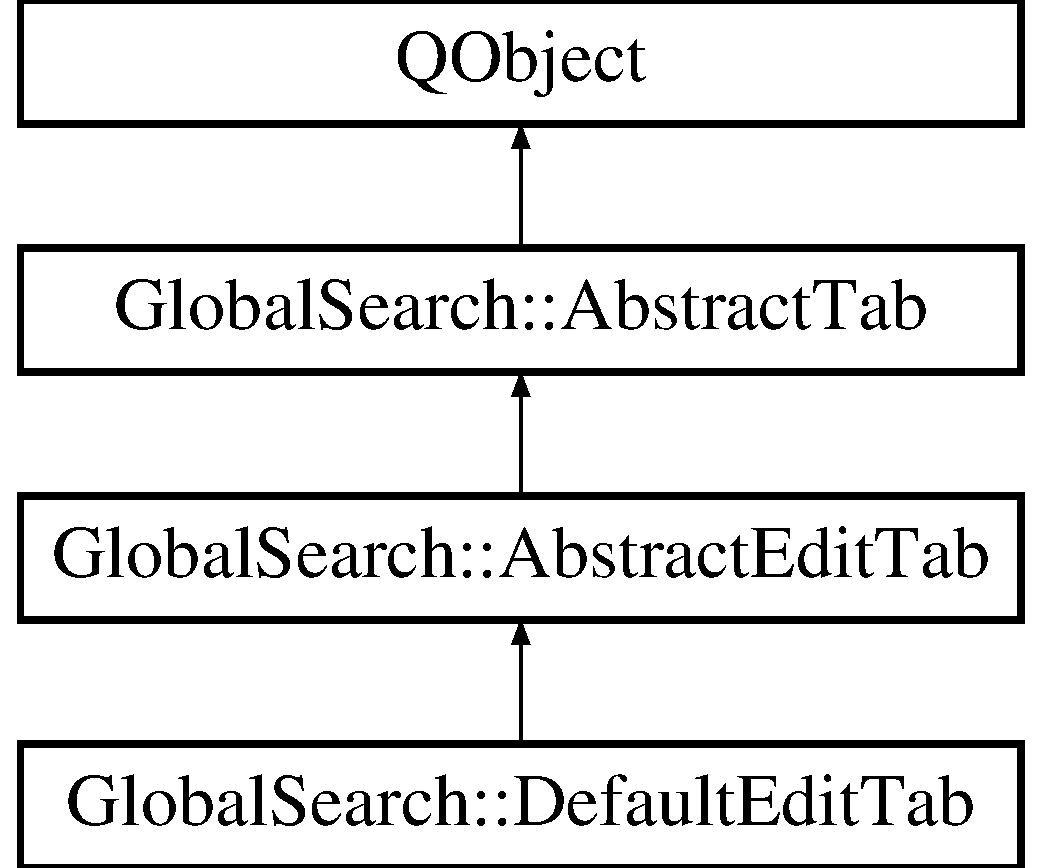
\includegraphics[height=4.000000cm]{classGlobalSearch_1_1AbstractEditTab}
\end{center}
\end{figure}
\subsubsection*{Public Slots}
\begin{DoxyCompactItemize}
\item 
virtual void \hyperlink{classGlobalSearch_1_1AbstractEditTab_a450c63567ac48b329469b2c380ff46a4}{lock\+G\+U\+I} ()
\item 
virtual void \hyperlink{classGlobalSearch_1_1AbstractEditTab_ae34c4af22aa9a04eebc3a4a4a284da53}{update\+G\+U\+I} ()
\item 
virtual void \hyperlink{classGlobalSearch_1_1AbstractEditTab_a19292ce55de31e989deee2b166c188d1}{update\+Edit\+Widget} ()
\item 
virtual void \hyperlink{classGlobalSearch_1_1AbstractEditTab_a19d5d4e568a67e46cc6431ba8c4199d0}{show\+Help} ()
\item 
virtual void \hyperlink{classGlobalSearch_1_1AbstractEditTab_a27965a0c57832b480b6663e786950e7d}{save\+Current\+Template} ()
\item 
virtual void \hyperlink{classGlobalSearch_1_1AbstractEditTab_ac973d18ed4a3c2d4ed8392a1fc8bed10}{populate\+Opt\+Step\+List} ()
\item 
virtual void \hyperlink{classGlobalSearch_1_1AbstractEditTab_ae37c49f896c0d668d48ef9bcae90dcf7}{populate\+Templates} ()
\item 
virtual void \hyperlink{classGlobalSearch_1_1AbstractEditTab_ae86997d35f9d05458638766b4378b92d}{append\+Opt\+Step} ()
\item 
virtual void \hyperlink{classGlobalSearch_1_1AbstractEditTab_a5507b5aaa5021085a57d1be72b71d975}{remove\+Current\+Opt\+Step} ()
\item 
virtual void \hyperlink{classGlobalSearch_1_1AbstractEditTab_a5ff01d9316ca927b7cf75d7a6720a793}{save\+Scheme} ()
\item 
virtual void \hyperlink{classGlobalSearch_1_1AbstractEditTab_a0b0d6a412e3b73113a0e84f6a86c0a8c}{load\+Scheme} ()
\item 
virtual Q\+String\+List \hyperlink{classGlobalSearch_1_1AbstractEditTab_a78c72c6174761b4c95eb4d512042120c}{get\+Template\+Names} ()
\end{DoxyCompactItemize}
\subsubsection*{Signals}
\begin{DoxyCompactItemize}
\item 
void \hyperlink{classGlobalSearch_1_1AbstractEditTab_a439d2f12f3121c30adf8f3375b631dee}{optimizer\+Changed} (\hyperlink{classGlobalSearch_1_1Optimizer}{Optimizer} $\ast$)
\item 
void \hyperlink{classGlobalSearch_1_1AbstractEditTab_a069c8370545d5fbde59b7634ba6bb621}{queue\+Interface\+Changed} (\hyperlink{classGlobalSearch_1_1QueueInterface}{Queue\+Interface} $\ast$)
\end{DoxyCompactItemize}
\subsubsection*{Public Member Functions}
\begin{DoxyCompactItemize}
\item 
\hyperlink{classGlobalSearch_1_1AbstractEditTab_a7c6f355f4e1ee393bb2dd93425e6f02a}{Abstract\+Edit\+Tab} (\hyperlink{classGlobalSearch_1_1AbstractDialog}{Abstract\+Dialog} $\ast$parent, \hyperlink{classGlobalSearch_1_1OptBase}{Opt\+Base} $\ast$p)
\item 
virtual \hyperlink{classGlobalSearch_1_1AbstractEditTab_ab4d202689e2018ad8db8b23a485d091d}{$\sim$\+Abstract\+Edit\+Tab} ()
\end{DoxyCompactItemize}
\subsubsection*{Protected Slots}
\begin{DoxyCompactItemize}
\item 
virtual void \hyperlink{classGlobalSearch_1_1AbstractEditTab_afb9fd8fbcf71d7287a8117ce4d75a00b}{initialize} ()
\item 
virtual void \hyperlink{classGlobalSearch_1_1AbstractEditTab_a3c241c0807a7f1dff4e75a7d9f2354fc}{update\+User\+Values} ()
\item 
virtual void \hyperlink{classGlobalSearch_1_1AbstractEditTab_aec415636f7b9aa295f8ae6d9a9035184}{update\+Queue\+Interface} ()
\item 
virtual void \hyperlink{classGlobalSearch_1_1AbstractEditTab_ad92c42eafb4b2bf681f3032148083441}{update\+Optimizer} ()
\item 
virtual void \hyperlink{classGlobalSearch_1_1AbstractEditTab_a4bd14eb377b74813bfc1474b92432567}{configure\+Queue\+Interface} ()
\item 
virtual void \hyperlink{classGlobalSearch_1_1AbstractEditTab_a4cc539eb78a2bcb984e46f73cbe2dfcd}{configure\+Optimizer} ()
\end{DoxyCompactItemize}
\subsubsection*{Protected Attributes}
\begin{DoxyCompactItemize}
\item 
Q\+List$<$ \hyperlink{classGlobalSearch_1_1Optimizer}{Optimizer} $\ast$ $>$ \hyperlink{classGlobalSearch_1_1AbstractEditTab_a91f1cbcdf3321b4502aaa11074559eba}{m\+\_\+optimizers}
\item 
Q\+List$<$ \hyperlink{classGlobalSearch_1_1QueueInterface}{Queue\+Interface} $\ast$ $>$ \hyperlink{classGlobalSearch_1_1AbstractEditTab_a364845072bfc0409a145c1cd6b60a60a}{m\+\_\+queue\+Interfaces}
\item 
\hypertarget{classGlobalSearch_1_1AbstractEditTab_af8be46a29c5959f04b5686cf2b222245}{}Q\+Combo\+Box $\ast$ \hyperlink{classGlobalSearch_1_1AbstractEditTab_af8be46a29c5959f04b5686cf2b222245}{ui\+\_\+combo\+\_\+queue\+Interfaces}\label{classGlobalSearch_1_1AbstractEditTab_af8be46a29c5959f04b5686cf2b222245}

\begin{DoxyCompactList}\small\item\em Cached G\+U\+I pointer. This is set in \hyperlink{classGlobalSearch_1_1DefaultEditTab}{Default\+Edit\+Tab}. \end{DoxyCompactList}\item 
\hypertarget{classGlobalSearch_1_1AbstractEditTab_a8145b8270f711300f397d39bfd9e54c4}{}Q\+Combo\+Box $\ast$ \hyperlink{classGlobalSearch_1_1AbstractEditTab_a8145b8270f711300f397d39bfd9e54c4}{ui\+\_\+combo\+\_\+optimizers}\label{classGlobalSearch_1_1AbstractEditTab_a8145b8270f711300f397d39bfd9e54c4}

\begin{DoxyCompactList}\small\item\em Cached G\+U\+I pointer. This is set in \hyperlink{classGlobalSearch_1_1DefaultEditTab}{Default\+Edit\+Tab}. \end{DoxyCompactList}\item 
\hypertarget{classGlobalSearch_1_1AbstractEditTab_afb3ed174abbd52491c89a76a7d749148}{}Q\+Combo\+Box $\ast$ \hyperlink{classGlobalSearch_1_1AbstractEditTab_afb3ed174abbd52491c89a76a7d749148}{ui\+\_\+combo\+\_\+templates}\label{classGlobalSearch_1_1AbstractEditTab_afb3ed174abbd52491c89a76a7d749148}

\begin{DoxyCompactList}\small\item\em Cached G\+U\+I pointer. This is set in \hyperlink{classGlobalSearch_1_1DefaultEditTab}{Default\+Edit\+Tab}. \end{DoxyCompactList}\item 
\hypertarget{classGlobalSearch_1_1AbstractEditTab_a5d584e064980b7b67f48d91b9236401d}{}Q\+Line\+Edit $\ast$ \hyperlink{classGlobalSearch_1_1AbstractEditTab_a5d584e064980b7b67f48d91b9236401d}{ui\+\_\+edit\+\_\+user1}\label{classGlobalSearch_1_1AbstractEditTab_a5d584e064980b7b67f48d91b9236401d}

\begin{DoxyCompactList}\small\item\em Cached G\+U\+I pointer. This is set in \hyperlink{classGlobalSearch_1_1DefaultEditTab}{Default\+Edit\+Tab}. \end{DoxyCompactList}\item 
\hypertarget{classGlobalSearch_1_1AbstractEditTab_a75db8027d5940557d102eecb3b161875}{}Q\+Line\+Edit $\ast$ \hyperlink{classGlobalSearch_1_1AbstractEditTab_a75db8027d5940557d102eecb3b161875}{ui\+\_\+edit\+\_\+user2}\label{classGlobalSearch_1_1AbstractEditTab_a75db8027d5940557d102eecb3b161875}

\begin{DoxyCompactList}\small\item\em Cached G\+U\+I pointer. This is set in \hyperlink{classGlobalSearch_1_1DefaultEditTab}{Default\+Edit\+Tab}. \end{DoxyCompactList}\item 
\hypertarget{classGlobalSearch_1_1AbstractEditTab_a7aaeb62e42fecda530bde483bbb7d8bc}{}Q\+Line\+Edit $\ast$ \hyperlink{classGlobalSearch_1_1AbstractEditTab_a7aaeb62e42fecda530bde483bbb7d8bc}{ui\+\_\+edit\+\_\+user3}\label{classGlobalSearch_1_1AbstractEditTab_a7aaeb62e42fecda530bde483bbb7d8bc}

\begin{DoxyCompactList}\small\item\em Cached G\+U\+I pointer. This is set in \hyperlink{classGlobalSearch_1_1DefaultEditTab}{Default\+Edit\+Tab}. \end{DoxyCompactList}\item 
\hypertarget{classGlobalSearch_1_1AbstractEditTab_a659f38ccad4e97c2c0a31847e9d4a51b}{}Q\+Line\+Edit $\ast$ \hyperlink{classGlobalSearch_1_1AbstractEditTab_a659f38ccad4e97c2c0a31847e9d4a51b}{ui\+\_\+edit\+\_\+user4}\label{classGlobalSearch_1_1AbstractEditTab_a659f38ccad4e97c2c0a31847e9d4a51b}

\begin{DoxyCompactList}\small\item\em Cached G\+U\+I pointer. This is set in \hyperlink{classGlobalSearch_1_1DefaultEditTab}{Default\+Edit\+Tab}. \end{DoxyCompactList}\item 
\hypertarget{classGlobalSearch_1_1AbstractEditTab_a9e43a02e109c453cd8df4ed9604885c7}{}Q\+List\+Widget $\ast$ \hyperlink{classGlobalSearch_1_1AbstractEditTab_a9e43a02e109c453cd8df4ed9604885c7}{ui\+\_\+list\+\_\+edit}\label{classGlobalSearch_1_1AbstractEditTab_a9e43a02e109c453cd8df4ed9604885c7}

\begin{DoxyCompactList}\small\item\em Cached G\+U\+I pointer. This is set in \hyperlink{classGlobalSearch_1_1DefaultEditTab}{Default\+Edit\+Tab}. \end{DoxyCompactList}\item 
\hypertarget{classGlobalSearch_1_1AbstractEditTab_a4635dc6d48af05e1dfb59b2a901ab80d}{}Q\+List\+Widget $\ast$ \hyperlink{classGlobalSearch_1_1AbstractEditTab_a4635dc6d48af05e1dfb59b2a901ab80d}{ui\+\_\+list\+\_\+opt\+Step}\label{classGlobalSearch_1_1AbstractEditTab_a4635dc6d48af05e1dfb59b2a901ab80d}

\begin{DoxyCompactList}\small\item\em Cached G\+U\+I pointer. This is set in \hyperlink{classGlobalSearch_1_1DefaultEditTab}{Default\+Edit\+Tab}. \end{DoxyCompactList}\item 
\hypertarget{classGlobalSearch_1_1AbstractEditTab_a8c5e86839aff6f2e437178101cce5d01}{}Q\+Push\+Button $\ast$ \hyperlink{classGlobalSearch_1_1AbstractEditTab_a8c5e86839aff6f2e437178101cce5d01}{ui\+\_\+push\+\_\+add}\label{classGlobalSearch_1_1AbstractEditTab_a8c5e86839aff6f2e437178101cce5d01}

\begin{DoxyCompactList}\small\item\em Cached G\+U\+I pointer. This is set in \hyperlink{classGlobalSearch_1_1DefaultEditTab}{Default\+Edit\+Tab}. \end{DoxyCompactList}\item 
\hypertarget{classGlobalSearch_1_1AbstractEditTab_a700455d26872a053bec69a10b7ddc2b4}{}Q\+Push\+Button $\ast$ \hyperlink{classGlobalSearch_1_1AbstractEditTab_a700455d26872a053bec69a10b7ddc2b4}{ui\+\_\+push\+\_\+help}\label{classGlobalSearch_1_1AbstractEditTab_a700455d26872a053bec69a10b7ddc2b4}

\begin{DoxyCompactList}\small\item\em Cached G\+U\+I pointer. This is set in \hyperlink{classGlobalSearch_1_1DefaultEditTab}{Default\+Edit\+Tab}. \end{DoxyCompactList}\item 
\hypertarget{classGlobalSearch_1_1AbstractEditTab_a7c4e25039853ec2c346b9d58d6a4dd73}{}Q\+Push\+Button $\ast$ \hyperlink{classGlobalSearch_1_1AbstractEditTab_a7c4e25039853ec2c346b9d58d6a4dd73}{ui\+\_\+push\+\_\+load\+Scheme}\label{classGlobalSearch_1_1AbstractEditTab_a7c4e25039853ec2c346b9d58d6a4dd73}

\begin{DoxyCompactList}\small\item\em Cached G\+U\+I pointer. This is set in \hyperlink{classGlobalSearch_1_1DefaultEditTab}{Default\+Edit\+Tab}. \end{DoxyCompactList}\item 
\hypertarget{classGlobalSearch_1_1AbstractEditTab_af9d6d07961a9d1bf1a8dcaa9b5f0835c}{}Q\+Push\+Button $\ast$ \hyperlink{classGlobalSearch_1_1AbstractEditTab_af9d6d07961a9d1bf1a8dcaa9b5f0835c}{ui\+\_\+push\+\_\+optimizer\+Config}\label{classGlobalSearch_1_1AbstractEditTab_af9d6d07961a9d1bf1a8dcaa9b5f0835c}

\begin{DoxyCompactList}\small\item\em Cached G\+U\+I pointer. This is set in \hyperlink{classGlobalSearch_1_1DefaultEditTab}{Default\+Edit\+Tab}. \end{DoxyCompactList}\item 
\hypertarget{classGlobalSearch_1_1AbstractEditTab_afa96b5d51634e8273f3db35d419b79a7}{}Q\+Push\+Button $\ast$ \hyperlink{classGlobalSearch_1_1AbstractEditTab_afa96b5d51634e8273f3db35d419b79a7}{ui\+\_\+push\+\_\+queue\+Interface\+Config}\label{classGlobalSearch_1_1AbstractEditTab_afa96b5d51634e8273f3db35d419b79a7}

\begin{DoxyCompactList}\small\item\em Cached G\+U\+I pointer. This is set in \hyperlink{classGlobalSearch_1_1DefaultEditTab}{Default\+Edit\+Tab}. \end{DoxyCompactList}\item 
\hypertarget{classGlobalSearch_1_1AbstractEditTab_a962cb890fe6a7028229e5ac6ffcc9872}{}Q\+Push\+Button $\ast$ \hyperlink{classGlobalSearch_1_1AbstractEditTab_a962cb890fe6a7028229e5ac6ffcc9872}{ui\+\_\+push\+\_\+remove}\label{classGlobalSearch_1_1AbstractEditTab_a962cb890fe6a7028229e5ac6ffcc9872}

\begin{DoxyCompactList}\small\item\em Cached G\+U\+I pointer. This is set in \hyperlink{classGlobalSearch_1_1DefaultEditTab}{Default\+Edit\+Tab}. \end{DoxyCompactList}\item 
\hypertarget{classGlobalSearch_1_1AbstractEditTab_a8ccc45a84048faa0b5bde84571fda19e}{}Q\+Push\+Button $\ast$ \hyperlink{classGlobalSearch_1_1AbstractEditTab_a8ccc45a84048faa0b5bde84571fda19e}{ui\+\_\+push\+\_\+save\+Scheme}\label{classGlobalSearch_1_1AbstractEditTab_a8ccc45a84048faa0b5bde84571fda19e}

\begin{DoxyCompactList}\small\item\em Cached G\+U\+I pointer. This is set in \hyperlink{classGlobalSearch_1_1DefaultEditTab}{Default\+Edit\+Tab}. \end{DoxyCompactList}\item 
\hypertarget{classGlobalSearch_1_1AbstractEditTab_affbc19b0e29c3f0aab22dc8f2a616c1f}{}Q\+Text\+Edit $\ast$ \hyperlink{classGlobalSearch_1_1AbstractEditTab_affbc19b0e29c3f0aab22dc8f2a616c1f}{ui\+\_\+edit\+\_\+edit}\label{classGlobalSearch_1_1AbstractEditTab_affbc19b0e29c3f0aab22dc8f2a616c1f}

\begin{DoxyCompactList}\small\item\em Cached G\+U\+I pointer. This is set in \hyperlink{classGlobalSearch_1_1DefaultEditTab}{Default\+Edit\+Tab}. \end{DoxyCompactList}\end{DoxyCompactItemize}


\subsubsection{Detailed Description}
Abstract class implementing a template editor. 

\begin{DoxyAuthor}{Author}
David C. Lonie 
\end{DoxyAuthor}


Definition at line 45 of file abstractedittab.\+h.



\subsubsection{Constructor \& Destructor Documentation}
\hypertarget{classGlobalSearch_1_1AbstractEditTab_a7c6f355f4e1ee393bb2dd93425e6f02a}{}\index{Global\+Search\+::\+Abstract\+Edit\+Tab@{Global\+Search\+::\+Abstract\+Edit\+Tab}!Abstract\+Edit\+Tab@{Abstract\+Edit\+Tab}}
\index{Abstract\+Edit\+Tab@{Abstract\+Edit\+Tab}!Global\+Search\+::\+Abstract\+Edit\+Tab@{Global\+Search\+::\+Abstract\+Edit\+Tab}}
\paragraph[{Abstract\+Edit\+Tab}]{\setlength{\rightskip}{0pt plus 5cm}Global\+Search\+::\+Abstract\+Edit\+Tab\+::\+Abstract\+Edit\+Tab (
\begin{DoxyParamCaption}
\item[{{\bf Abstract\+Dialog} $\ast$}]{parent, }
\item[{{\bf Opt\+Base} $\ast$}]{p}
\end{DoxyParamCaption}
)\hspace{0.3cm}{\ttfamily [explicit]}}\label{classGlobalSearch_1_1AbstractEditTab_a7c6f355f4e1ee393bb2dd93425e6f02a}
Constructor


\begin{DoxyParams}{Parameters}
{\em parent} & \hyperlink{classGlobalSearch_1_1AbstractDialog}{Abstract\+Dialog} that will use this tab \\
\hline
{\em p} & Associated \hyperlink{classGlobalSearch_1_1OptBase}{Opt\+Base} \\
\hline
\end{DoxyParams}


Definition at line 35 of file abstractedittab.\+cpp.

\hypertarget{classGlobalSearch_1_1AbstractEditTab_ab4d202689e2018ad8db8b23a485d091d}{}\index{Global\+Search\+::\+Abstract\+Edit\+Tab@{Global\+Search\+::\+Abstract\+Edit\+Tab}!````~Abstract\+Edit\+Tab@{$\sim$\+Abstract\+Edit\+Tab}}
\index{````~Abstract\+Edit\+Tab@{$\sim$\+Abstract\+Edit\+Tab}!Global\+Search\+::\+Abstract\+Edit\+Tab@{Global\+Search\+::\+Abstract\+Edit\+Tab}}
\paragraph[{$\sim$\+Abstract\+Edit\+Tab}]{\setlength{\rightskip}{0pt plus 5cm}Global\+Search\+::\+Abstract\+Edit\+Tab\+::$\sim$\+Abstract\+Edit\+Tab (
\begin{DoxyParamCaption}
{}
\end{DoxyParamCaption}
)\hspace{0.3cm}{\ttfamily [virtual]}}\label{classGlobalSearch_1_1AbstractEditTab_ab4d202689e2018ad8db8b23a485d091d}
Destructor 

Definition at line 148 of file abstractedittab.\+cpp.



\subsubsection{Member Function Documentation}
\hypertarget{classGlobalSearch_1_1AbstractEditTab_ae86997d35f9d05458638766b4378b92d}{}\index{Global\+Search\+::\+Abstract\+Edit\+Tab@{Global\+Search\+::\+Abstract\+Edit\+Tab}!append\+Opt\+Step@{append\+Opt\+Step}}
\index{append\+Opt\+Step@{append\+Opt\+Step}!Global\+Search\+::\+Abstract\+Edit\+Tab@{Global\+Search\+::\+Abstract\+Edit\+Tab}}
\paragraph[{append\+Opt\+Step}]{\setlength{\rightskip}{0pt plus 5cm}void Global\+Search\+::\+Abstract\+Edit\+Tab\+::append\+Opt\+Step (
\begin{DoxyParamCaption}
{}
\end{DoxyParamCaption}
)\hspace{0.3cm}{\ttfamily [virtual]}, {\ttfamily [slot]}}\label{classGlobalSearch_1_1AbstractEditTab_ae86997d35f9d05458638766b4378b92d}
Create a new optstep at the end of the optstep list. It will initialize using the currently selected optstep\textquotesingle{}s templates. 

Definition at line 411 of file abstractedittab.\+cpp.



References Global\+Search\+::\+Optimizer\+::get\+Number\+Of\+Opt\+Steps(), get\+Template\+Names(), Global\+Search\+::\+Abstract\+Tab\+::m\+\_\+opt, Global\+Search\+::\+Opt\+Base\+::optimizer(), populate\+Opt\+Step\+List(), and ui\+\_\+list\+\_\+opt\+Step.



Referenced by initialize().

\hypertarget{classGlobalSearch_1_1AbstractEditTab_a4cc539eb78a2bcb984e46f73cbe2dfcd}{}\index{Global\+Search\+::\+Abstract\+Edit\+Tab@{Global\+Search\+::\+Abstract\+Edit\+Tab}!configure\+Optimizer@{configure\+Optimizer}}
\index{configure\+Optimizer@{configure\+Optimizer}!Global\+Search\+::\+Abstract\+Edit\+Tab@{Global\+Search\+::\+Abstract\+Edit\+Tab}}
\paragraph[{configure\+Optimizer}]{\setlength{\rightskip}{0pt plus 5cm}void Global\+Search\+::\+Abstract\+Edit\+Tab\+::configure\+Optimizer (
\begin{DoxyParamCaption}
{}
\end{DoxyParamCaption}
)\hspace{0.3cm}{\ttfamily [protected]}, {\ttfamily [virtual]}, {\ttfamily [slot]}}\label{classGlobalSearch_1_1AbstractEditTab_a4cc539eb78a2bcb984e46f73cbe2dfcd}
Launch the \hyperlink{classGlobalSearch_1_1Optimizer}{Optimizer} configuration dialog. 

Definition at line 276 of file abstractedittab.\+cpp.



References Global\+Search\+::\+Optimizer\+::dialog(), Global\+Search\+::\+Optimizer\+::has\+Dialog(), Global\+Search\+::\+Abstract\+Tab\+::m\+\_\+opt, and Global\+Search\+::\+Opt\+Base\+::optimizer().



Referenced by initialize().

\hypertarget{classGlobalSearch_1_1AbstractEditTab_a4bd14eb377b74813bfc1474b92432567}{}\index{Global\+Search\+::\+Abstract\+Edit\+Tab@{Global\+Search\+::\+Abstract\+Edit\+Tab}!configure\+Queue\+Interface@{configure\+Queue\+Interface}}
\index{configure\+Queue\+Interface@{configure\+Queue\+Interface}!Global\+Search\+::\+Abstract\+Edit\+Tab@{Global\+Search\+::\+Abstract\+Edit\+Tab}}
\paragraph[{configure\+Queue\+Interface}]{\setlength{\rightskip}{0pt plus 5cm}void Global\+Search\+::\+Abstract\+Edit\+Tab\+::configure\+Queue\+Interface (
\begin{DoxyParamCaption}
{}
\end{DoxyParamCaption}
)\hspace{0.3cm}{\ttfamily [protected]}, {\ttfamily [virtual]}, {\ttfamily [slot]}}\label{classGlobalSearch_1_1AbstractEditTab_a4bd14eb377b74813bfc1474b92432567}
Launch the \hyperlink{classGlobalSearch_1_1QueueInterface}{Queue\+Interface} configuration dialog. 

Definition at line 264 of file abstractedittab.\+cpp.



References Global\+Search\+::\+Queue\+Interface\+::dialog(), Global\+Search\+::\+Queue\+Interface\+::has\+Dialog(), Global\+Search\+::\+Abstract\+Tab\+::m\+\_\+opt, and Global\+Search\+::\+Opt\+Base\+::queue\+Interface().



Referenced by initialize().

\hypertarget{classGlobalSearch_1_1AbstractEditTab_a78c72c6174761b4c95eb4d512042120c}{}\index{Global\+Search\+::\+Abstract\+Edit\+Tab@{Global\+Search\+::\+Abstract\+Edit\+Tab}!get\+Template\+Names@{get\+Template\+Names}}
\index{get\+Template\+Names@{get\+Template\+Names}!Global\+Search\+::\+Abstract\+Edit\+Tab@{Global\+Search\+::\+Abstract\+Edit\+Tab}}
\paragraph[{get\+Template\+Names}]{\setlength{\rightskip}{0pt plus 5cm}Q\+String\+List Global\+Search\+::\+Abstract\+Edit\+Tab\+::get\+Template\+Names (
\begin{DoxyParamCaption}
{}
\end{DoxyParamCaption}
)\hspace{0.3cm}{\ttfamily [virtual]}, {\ttfamily [slot]}}\label{classGlobalSearch_1_1AbstractEditTab_a78c72c6174761b4c95eb4d512042120c}
\begin{DoxyReturn}{Returns}
A list of the available template names for the current \hyperlink{classGlobalSearch_1_1QueueInterface}{Queue\+Interface} and \hyperlink{classGlobalSearch_1_1Optimizer}{Optimizer}. 
\end{DoxyReturn}


Definition at line 288 of file abstractedittab.\+cpp.



References Global\+Search\+::\+Queue\+Interface\+::get\+Template\+File\+Names(), Global\+Search\+::\+Optimizer\+::get\+Template\+Names(), Global\+Search\+::\+Abstract\+Tab\+::m\+\_\+is\+Initialized, Global\+Search\+::\+Abstract\+Tab\+::m\+\_\+opt, Global\+Search\+::\+Opt\+Base\+::optimizer(), and Global\+Search\+::\+Opt\+Base\+::queue\+Interface().



Referenced by append\+Opt\+Step(), populate\+Templates(), save\+Current\+Template(), and update\+Edit\+Widget().

\hypertarget{classGlobalSearch_1_1AbstractEditTab_afb9fd8fbcf71d7287a8117ce4d75a00b}{}\index{Global\+Search\+::\+Abstract\+Edit\+Tab@{Global\+Search\+::\+Abstract\+Edit\+Tab}!initialize@{initialize}}
\index{initialize@{initialize}!Global\+Search\+::\+Abstract\+Edit\+Tab@{Global\+Search\+::\+Abstract\+Edit\+Tab}}
\paragraph[{initialize}]{\setlength{\rightskip}{0pt plus 5cm}void Global\+Search\+::\+Abstract\+Edit\+Tab\+::initialize (
\begin{DoxyParamCaption}
{}
\end{DoxyParamCaption}
)\hspace{0.3cm}{\ttfamily [protected]}, {\ttfamily [virtual]}, {\ttfamily [slot]}}\label{classGlobalSearch_1_1AbstractEditTab_afb9fd8fbcf71d7287a8117ce4d75a00b}
Create connections and initialize G\+U\+I. 

Definition at line 54 of file abstractedittab.\+cpp.



References append\+Opt\+Step(), configure\+Optimizer(), configure\+Queue\+Interface(), Global\+Search\+::\+Abstract\+Tab\+::initialize(), load\+Scheme(), Global\+Search\+::\+Abstract\+Tab\+::m\+\_\+dialog, Global\+Search\+::\+Abstract\+Tab\+::m\+\_\+opt, m\+\_\+optimizers, m\+\_\+queue\+Interfaces, optimizer\+Changed(), populate\+Opt\+Step\+List(), populate\+Templates(), queue\+Interface\+Changed(), remove\+Current\+Opt\+Step(), save\+Current\+Template(), save\+Scheme(), show\+Help(), ui\+\_\+combo\+\_\+optimizers, ui\+\_\+combo\+\_\+queue\+Interfaces, ui\+\_\+combo\+\_\+templates, ui\+\_\+edit\+\_\+edit, ui\+\_\+edit\+\_\+user1, ui\+\_\+edit\+\_\+user2, ui\+\_\+edit\+\_\+user3, ui\+\_\+edit\+\_\+user4, ui\+\_\+list\+\_\+opt\+Step, ui\+\_\+push\+\_\+add, ui\+\_\+push\+\_\+help, ui\+\_\+push\+\_\+load\+Scheme, ui\+\_\+push\+\_\+optimizer\+Config, ui\+\_\+push\+\_\+queue\+Interface\+Config, ui\+\_\+push\+\_\+remove, ui\+\_\+push\+\_\+save\+Scheme, update\+Edit\+Widget(), update\+G\+U\+I(), update\+Optimizer(), update\+Queue\+Interface(), and update\+User\+Values().



Referenced by Global\+Search\+::\+Default\+Edit\+Tab\+::initialize().

\hypertarget{classGlobalSearch_1_1AbstractEditTab_a0b0d6a412e3b73113a0e84f6a86c0a8c}{}\index{Global\+Search\+::\+Abstract\+Edit\+Tab@{Global\+Search\+::\+Abstract\+Edit\+Tab}!load\+Scheme@{load\+Scheme}}
\index{load\+Scheme@{load\+Scheme}!Global\+Search\+::\+Abstract\+Edit\+Tab@{Global\+Search\+::\+Abstract\+Edit\+Tab}}
\paragraph[{load\+Scheme}]{\setlength{\rightskip}{0pt plus 5cm}void Global\+Search\+::\+Abstract\+Edit\+Tab\+::load\+Scheme (
\begin{DoxyParamCaption}
{}
\end{DoxyParamCaption}
)\hspace{0.3cm}{\ttfamily [virtual]}, {\ttfamily [slot]}}\label{classGlobalSearch_1_1AbstractEditTab_a0b0d6a412e3b73113a0e84f6a86c0a8c}
Load an optimization scheme from a file. This will prompt the user for the filename. 

Definition at line 468 of file abstractedittab.\+cpp.



References Global\+Search\+::\+Opt\+Base\+::get\+I\+D\+String(), Global\+Search\+::\+Abstract\+Tab\+::m\+\_\+opt, and Global\+Search\+::\+Abstract\+Tab\+::read\+Settings().



Referenced by initialize().

\hypertarget{classGlobalSearch_1_1AbstractEditTab_a450c63567ac48b329469b2c380ff46a4}{}\index{Global\+Search\+::\+Abstract\+Edit\+Tab@{Global\+Search\+::\+Abstract\+Edit\+Tab}!lock\+G\+U\+I@{lock\+G\+U\+I}}
\index{lock\+G\+U\+I@{lock\+G\+U\+I}!Global\+Search\+::\+Abstract\+Edit\+Tab@{Global\+Search\+::\+Abstract\+Edit\+Tab}}
\paragraph[{lock\+G\+U\+I}]{\setlength{\rightskip}{0pt plus 5cm}void Global\+Search\+::\+Abstract\+Edit\+Tab\+::lock\+G\+U\+I (
\begin{DoxyParamCaption}
{}
\end{DoxyParamCaption}
)\hspace{0.3cm}{\ttfamily [virtual]}, {\ttfamily [slot]}}\label{classGlobalSearch_1_1AbstractEditTab_a450c63567ac48b329469b2c380ff46a4}
Lock G\+U\+I elements that shouldn\textquotesingle{}t change once the search begins. 

Definition at line 195 of file abstractedittab.\+cpp.



References ui\+\_\+combo\+\_\+optimizers, and ui\+\_\+combo\+\_\+queue\+Interfaces.

\hypertarget{classGlobalSearch_1_1AbstractEditTab_a439d2f12f3121c30adf8f3375b631dee}{}\index{Global\+Search\+::\+Abstract\+Edit\+Tab@{Global\+Search\+::\+Abstract\+Edit\+Tab}!optimizer\+Changed@{optimizer\+Changed}}
\index{optimizer\+Changed@{optimizer\+Changed}!Global\+Search\+::\+Abstract\+Edit\+Tab@{Global\+Search\+::\+Abstract\+Edit\+Tab}}
\paragraph[{optimizer\+Changed}]{\setlength{\rightskip}{0pt plus 5cm}void Global\+Search\+::\+Abstract\+Edit\+Tab\+::optimizer\+Changed (
\begin{DoxyParamCaption}
\item[{{\bf Optimizer} $\ast$}]{}
\end{DoxyParamCaption}
)\hspace{0.3cm}{\ttfamily [signal]}}\label{classGlobalSearch_1_1AbstractEditTab_a439d2f12f3121c30adf8f3375b631dee}
Emitted when the \hyperlink{classGlobalSearch_1_1Optimizer}{Optimizer} changes. 

Referenced by initialize(), and update\+Optimizer().

\hypertarget{classGlobalSearch_1_1AbstractEditTab_ac973d18ed4a3c2d4ed8392a1fc8bed10}{}\index{Global\+Search\+::\+Abstract\+Edit\+Tab@{Global\+Search\+::\+Abstract\+Edit\+Tab}!populate\+Opt\+Step\+List@{populate\+Opt\+Step\+List}}
\index{populate\+Opt\+Step\+List@{populate\+Opt\+Step\+List}!Global\+Search\+::\+Abstract\+Edit\+Tab@{Global\+Search\+::\+Abstract\+Edit\+Tab}}
\paragraph[{populate\+Opt\+Step\+List}]{\setlength{\rightskip}{0pt plus 5cm}void Global\+Search\+::\+Abstract\+Edit\+Tab\+::populate\+Opt\+Step\+List (
\begin{DoxyParamCaption}
{}
\end{DoxyParamCaption}
)\hspace{0.3cm}{\ttfamily [virtual]}, {\ttfamily [slot]}}\label{classGlobalSearch_1_1AbstractEditTab_ac973d18ed4a3c2d4ed8392a1fc8bed10}
Generate the list of optsteps. 

Definition at line 384 of file abstractedittab.\+cpp.



References Global\+Search\+::\+Optimizer\+::get\+Number\+Of\+Opt\+Steps(), Global\+Search\+::\+Abstract\+Tab\+::m\+\_\+is\+Initialized, Global\+Search\+::\+Abstract\+Tab\+::m\+\_\+opt, Global\+Search\+::\+Opt\+Base\+::optimizer(), Global\+Search\+::\+Opt\+Base\+::queue\+Interface(), and ui\+\_\+list\+\_\+opt\+Step.



Referenced by append\+Opt\+Step(), initialize(), remove\+Current\+Opt\+Step(), save\+Current\+Template(), update\+Edit\+Widget(), and update\+G\+U\+I().

\hypertarget{classGlobalSearch_1_1AbstractEditTab_ae37c49f896c0d668d48ef9bcae90dcf7}{}\index{Global\+Search\+::\+Abstract\+Edit\+Tab@{Global\+Search\+::\+Abstract\+Edit\+Tab}!populate\+Templates@{populate\+Templates}}
\index{populate\+Templates@{populate\+Templates}!Global\+Search\+::\+Abstract\+Edit\+Tab@{Global\+Search\+::\+Abstract\+Edit\+Tab}}
\paragraph[{populate\+Templates}]{\setlength{\rightskip}{0pt plus 5cm}void Global\+Search\+::\+Abstract\+Edit\+Tab\+::populate\+Templates (
\begin{DoxyParamCaption}
{}
\end{DoxyParamCaption}
)\hspace{0.3cm}{\ttfamily [virtual]}, {\ttfamily [slot]}}\label{classGlobalSearch_1_1AbstractEditTab_ae37c49f896c0d668d48ef9bcae90dcf7}
Fill the template selection combo using the template names for the current \hyperlink{classGlobalSearch_1_1QueueInterface}{Queue\+Interface} and \hyperlink{classGlobalSearch_1_1Optimizer}{Optimizer}. 

Definition at line 299 of file abstractedittab.\+cpp.



References get\+Template\+Names(), Global\+Search\+::\+Abstract\+Tab\+::m\+\_\+is\+Initialized, and ui\+\_\+combo\+\_\+templates.



Referenced by initialize(), and update\+G\+U\+I().

\hypertarget{classGlobalSearch_1_1AbstractEditTab_a069c8370545d5fbde59b7634ba6bb621}{}\index{Global\+Search\+::\+Abstract\+Edit\+Tab@{Global\+Search\+::\+Abstract\+Edit\+Tab}!queue\+Interface\+Changed@{queue\+Interface\+Changed}}
\index{queue\+Interface\+Changed@{queue\+Interface\+Changed}!Global\+Search\+::\+Abstract\+Edit\+Tab@{Global\+Search\+::\+Abstract\+Edit\+Tab}}
\paragraph[{queue\+Interface\+Changed}]{\setlength{\rightskip}{0pt plus 5cm}void Global\+Search\+::\+Abstract\+Edit\+Tab\+::queue\+Interface\+Changed (
\begin{DoxyParamCaption}
\item[{{\bf Queue\+Interface} $\ast$}]{}
\end{DoxyParamCaption}
)\hspace{0.3cm}{\ttfamily [signal]}}\label{classGlobalSearch_1_1AbstractEditTab_a069c8370545d5fbde59b7634ba6bb621}
Emitted when the \hyperlink{classGlobalSearch_1_1QueueInterface}{Queue\+Interface} changes. 

Referenced by initialize(), and update\+Queue\+Interface().

\hypertarget{classGlobalSearch_1_1AbstractEditTab_a5507b5aaa5021085a57d1be72b71d975}{}\index{Global\+Search\+::\+Abstract\+Edit\+Tab@{Global\+Search\+::\+Abstract\+Edit\+Tab}!remove\+Current\+Opt\+Step@{remove\+Current\+Opt\+Step}}
\index{remove\+Current\+Opt\+Step@{remove\+Current\+Opt\+Step}!Global\+Search\+::\+Abstract\+Edit\+Tab@{Global\+Search\+::\+Abstract\+Edit\+Tab}}
\paragraph[{remove\+Current\+Opt\+Step}]{\setlength{\rightskip}{0pt plus 5cm}void Global\+Search\+::\+Abstract\+Edit\+Tab\+::remove\+Current\+Opt\+Step (
\begin{DoxyParamCaption}
{}
\end{DoxyParamCaption}
)\hspace{0.3cm}{\ttfamily [virtual]}, {\ttfamily [slot]}}\label{classGlobalSearch_1_1AbstractEditTab_a5507b5aaa5021085a57d1be72b71d975}
Delete the currently selected optstep. 

Definition at line 435 of file abstractedittab.\+cpp.



References Global\+Search\+::\+Optimizer\+::get\+Number\+Of\+Opt\+Steps(), Global\+Search\+::\+Abstract\+Tab\+::m\+\_\+opt, Global\+Search\+::\+Opt\+Base\+::optimizer(), populate\+Opt\+Step\+List(), Global\+Search\+::\+Optimizer\+::remove\+All\+Templates\+For\+Opt\+Step(), and ui\+\_\+list\+\_\+opt\+Step.



Referenced by initialize().

\hypertarget{classGlobalSearch_1_1AbstractEditTab_a27965a0c57832b480b6663e786950e7d}{}\index{Global\+Search\+::\+Abstract\+Edit\+Tab@{Global\+Search\+::\+Abstract\+Edit\+Tab}!save\+Current\+Template@{save\+Current\+Template}}
\index{save\+Current\+Template@{save\+Current\+Template}!Global\+Search\+::\+Abstract\+Edit\+Tab@{Global\+Search\+::\+Abstract\+Edit\+Tab}}
\paragraph[{save\+Current\+Template}]{\setlength{\rightskip}{0pt plus 5cm}void Global\+Search\+::\+Abstract\+Edit\+Tab\+::save\+Current\+Template (
\begin{DoxyParamCaption}
{}
\end{DoxyParamCaption}
)\hspace{0.3cm}{\ttfamily [virtual]}, {\ttfamily [slot]}}\label{classGlobalSearch_1_1AbstractEditTab_a27965a0c57832b480b6663e786950e7d}
Save the text in the template editor to the appropriate template list. 

Definition at line 349 of file abstractedittab.\+cpp.



References Global\+Search\+::\+Optimizer\+::get\+Number\+Of\+Opt\+Steps(), get\+Template\+Names(), Global\+Search\+::\+Abstract\+Tab\+::m\+\_\+opt, Global\+Search\+::\+Opt\+Base\+::optimizer(), populate\+Opt\+Step\+List(), Global\+Search\+::\+Optimizer\+::set\+Template(), ui\+\_\+combo\+\_\+templates, ui\+\_\+edit\+\_\+edit, and ui\+\_\+list\+\_\+opt\+Step.



Referenced by initialize().

\hypertarget{classGlobalSearch_1_1AbstractEditTab_a5ff01d9316ca927b7cf75d7a6720a793}{}\index{Global\+Search\+::\+Abstract\+Edit\+Tab@{Global\+Search\+::\+Abstract\+Edit\+Tab}!save\+Scheme@{save\+Scheme}}
\index{save\+Scheme@{save\+Scheme}!Global\+Search\+::\+Abstract\+Edit\+Tab@{Global\+Search\+::\+Abstract\+Edit\+Tab}}
\paragraph[{save\+Scheme}]{\setlength{\rightskip}{0pt plus 5cm}void Global\+Search\+::\+Abstract\+Edit\+Tab\+::save\+Scheme (
\begin{DoxyParamCaption}
{}
\end{DoxyParamCaption}
)\hspace{0.3cm}{\ttfamily [virtual]}, {\ttfamily [slot]}}\label{classGlobalSearch_1_1AbstractEditTab_a5ff01d9316ca927b7cf75d7a6720a793}
Save the current optimization scheme. This will prompt for the user to specify the filename. 

Definition at line 447 of file abstractedittab.\+cpp.



References Global\+Search\+::\+Opt\+Base\+::get\+I\+D\+String(), Global\+Search\+::\+Optimizer\+::get\+I\+D\+String(), Global\+Search\+::\+Abstract\+Tab\+::m\+\_\+opt, Global\+Search\+::\+Opt\+Base\+::optimizer(), and Global\+Search\+::\+Abstract\+Tab\+::write\+Settings().



Referenced by initialize().

\hypertarget{classGlobalSearch_1_1AbstractEditTab_a19d5d4e568a67e46cc6431ba8c4199d0}{}\index{Global\+Search\+::\+Abstract\+Edit\+Tab@{Global\+Search\+::\+Abstract\+Edit\+Tab}!show\+Help@{show\+Help}}
\index{show\+Help@{show\+Help}!Global\+Search\+::\+Abstract\+Edit\+Tab@{Global\+Search\+::\+Abstract\+Edit\+Tab}}
\paragraph[{show\+Help}]{\setlength{\rightskip}{0pt plus 5cm}void Global\+Search\+::\+Abstract\+Edit\+Tab\+::show\+Help (
\begin{DoxyParamCaption}
{}
\end{DoxyParamCaption}
)\hspace{0.3cm}{\ttfamily [virtual]}, {\ttfamily [slot]}}\label{classGlobalSearch_1_1AbstractEditTab_a19d5d4e568a67e46cc6431ba8c4199d0}
Popup a message box displaying the keyword documentation. 

Definition at line 201 of file abstractedittab.\+cpp.



References Global\+Search\+::\+Opt\+Base\+::get\+Template\+Keyword\+Help(), Global\+Search\+::\+Abstract\+Tab\+::m\+\_\+dialog, and Global\+Search\+::\+Abstract\+Tab\+::m\+\_\+opt.



Referenced by initialize().

\hypertarget{classGlobalSearch_1_1AbstractEditTab_a19292ce55de31e989deee2b166c188d1}{}\index{Global\+Search\+::\+Abstract\+Edit\+Tab@{Global\+Search\+::\+Abstract\+Edit\+Tab}!update\+Edit\+Widget@{update\+Edit\+Widget}}
\index{update\+Edit\+Widget@{update\+Edit\+Widget}!Global\+Search\+::\+Abstract\+Edit\+Tab@{Global\+Search\+::\+Abstract\+Edit\+Tab}}
\paragraph[{update\+Edit\+Widget}]{\setlength{\rightskip}{0pt plus 5cm}void Global\+Search\+::\+Abstract\+Edit\+Tab\+::update\+Edit\+Widget (
\begin{DoxyParamCaption}
{}
\end{DoxyParamCaption}
)\hspace{0.3cm}{\ttfamily [virtual]}, {\ttfamily [slot]}}\label{classGlobalSearch_1_1AbstractEditTab_a19292ce55de31e989deee2b166c188d1}
Display the currently selected template in the text editor. 

Definition at line 311 of file abstractedittab.\+cpp.



References Global\+Search\+::\+Optimizer\+::get\+Number\+Of\+Opt\+Steps(), Global\+Search\+::\+Optimizer\+::get\+Template(), get\+Template\+Names(), Global\+Search\+::\+Abstract\+Tab\+::m\+\_\+is\+Initialized, Global\+Search\+::\+Abstract\+Tab\+::m\+\_\+opt, Global\+Search\+::\+Opt\+Base\+::optimizer(), populate\+Opt\+Step\+List(), ui\+\_\+combo\+\_\+templates, ui\+\_\+edit\+\_\+edit, ui\+\_\+list\+\_\+edit, and ui\+\_\+list\+\_\+opt\+Step.



Referenced by initialize(), and update\+G\+U\+I().

\hypertarget{classGlobalSearch_1_1AbstractEditTab_ae34c4af22aa9a04eebc3a4a4a284da53}{}\index{Global\+Search\+::\+Abstract\+Edit\+Tab@{Global\+Search\+::\+Abstract\+Edit\+Tab}!update\+G\+U\+I@{update\+G\+U\+I}}
\index{update\+G\+U\+I@{update\+G\+U\+I}!Global\+Search\+::\+Abstract\+Edit\+Tab@{Global\+Search\+::\+Abstract\+Edit\+Tab}}
\paragraph[{update\+G\+U\+I}]{\setlength{\rightskip}{0pt plus 5cm}void Global\+Search\+::\+Abstract\+Edit\+Tab\+::update\+G\+U\+I (
\begin{DoxyParamCaption}
{}
\end{DoxyParamCaption}
)\hspace{0.3cm}{\ttfamily [virtual]}, {\ttfamily [slot]}}\label{classGlobalSearch_1_1AbstractEditTab_ae34c4af22aa9a04eebc3a4a4a284da53}
Force a refresh of the G\+U\+I elements using the internal state. 

Definition at line 152 of file abstractedittab.\+cpp.



References Global\+Search\+::\+Optimizer\+::get\+User1(), Global\+Search\+::\+Optimizer\+::get\+User2(), Global\+Search\+::\+Optimizer\+::get\+User3(), Global\+Search\+::\+Optimizer\+::get\+User4(), Global\+Search\+::\+Queue\+Interface\+::has\+Dialog(), Global\+Search\+::\+Abstract\+Tab\+::m\+\_\+is\+Initialized, Global\+Search\+::\+Abstract\+Tab\+::m\+\_\+opt, m\+\_\+optimizers, m\+\_\+queue\+Interfaces, Global\+Search\+::\+Opt\+Base\+::optimizer(), populate\+Opt\+Step\+List(), populate\+Templates(), Global\+Search\+::\+Opt\+Base\+::queue\+Interface(), ui\+\_\+combo\+\_\+optimizers, ui\+\_\+combo\+\_\+queue\+Interfaces, ui\+\_\+edit\+\_\+user1, ui\+\_\+edit\+\_\+user2, ui\+\_\+edit\+\_\+user3, ui\+\_\+edit\+\_\+user4, ui\+\_\+push\+\_\+queue\+Interface\+Config, and update\+Edit\+Widget().



Referenced by initialize().

\hypertarget{classGlobalSearch_1_1AbstractEditTab_ad92c42eafb4b2bf681f3032148083441}{}\index{Global\+Search\+::\+Abstract\+Edit\+Tab@{Global\+Search\+::\+Abstract\+Edit\+Tab}!update\+Optimizer@{update\+Optimizer}}
\index{update\+Optimizer@{update\+Optimizer}!Global\+Search\+::\+Abstract\+Edit\+Tab@{Global\+Search\+::\+Abstract\+Edit\+Tab}}
\paragraph[{update\+Optimizer}]{\setlength{\rightskip}{0pt plus 5cm}void Global\+Search\+::\+Abstract\+Edit\+Tab\+::update\+Optimizer (
\begin{DoxyParamCaption}
{}
\end{DoxyParamCaption}
)\hspace{0.3cm}{\ttfamily [protected]}, {\ttfamily [virtual]}, {\ttfamily [slot]}}\label{classGlobalSearch_1_1AbstractEditTab_ad92c42eafb4b2bf681f3032148083441}
Determine the currently selected \hyperlink{classGlobalSearch_1_1Optimizer}{Optimizer} and emit optimizer\+Changed if it differs from the current one. 

Definition at line 236 of file abstractedittab.\+cpp.



References Global\+Search\+::\+Optimizer\+::has\+Dialog(), Global\+Search\+::\+Abstract\+Tab\+::m\+\_\+opt, m\+\_\+optimizers, Global\+Search\+::\+Opt\+Base\+::optimizer(), optimizer\+Changed(), ui\+\_\+combo\+\_\+optimizers, and ui\+\_\+push\+\_\+optimizer\+Config.



Referenced by initialize().

\hypertarget{classGlobalSearch_1_1AbstractEditTab_aec415636f7b9aa295f8ae6d9a9035184}{}\index{Global\+Search\+::\+Abstract\+Edit\+Tab@{Global\+Search\+::\+Abstract\+Edit\+Tab}!update\+Queue\+Interface@{update\+Queue\+Interface}}
\index{update\+Queue\+Interface@{update\+Queue\+Interface}!Global\+Search\+::\+Abstract\+Edit\+Tab@{Global\+Search\+::\+Abstract\+Edit\+Tab}}
\paragraph[{update\+Queue\+Interface}]{\setlength{\rightskip}{0pt plus 5cm}void Global\+Search\+::\+Abstract\+Edit\+Tab\+::update\+Queue\+Interface (
\begin{DoxyParamCaption}
{}
\end{DoxyParamCaption}
)\hspace{0.3cm}{\ttfamily [protected]}, {\ttfamily [virtual]}, {\ttfamily [slot]}}\label{classGlobalSearch_1_1AbstractEditTab_aec415636f7b9aa295f8ae6d9a9035184}
Determine the currently selected \hyperlink{classGlobalSearch_1_1QueueInterface}{Queue\+Interface} and emit queue\+Interface\+Changed if it differs from the current one. 

Definition at line 208 of file abstractedittab.\+cpp.



References Global\+Search\+::\+Queue\+Interface\+::has\+Dialog(), Global\+Search\+::\+Abstract\+Tab\+::m\+\_\+opt, m\+\_\+queue\+Interfaces, Global\+Search\+::\+Opt\+Base\+::queue\+Interface(), queue\+Interface\+Changed(), ui\+\_\+combo\+\_\+queue\+Interfaces, and ui\+\_\+push\+\_\+queue\+Interface\+Config.



Referenced by initialize().

\hypertarget{classGlobalSearch_1_1AbstractEditTab_a3c241c0807a7f1dff4e75a7d9f2354fc}{}\index{Global\+Search\+::\+Abstract\+Edit\+Tab@{Global\+Search\+::\+Abstract\+Edit\+Tab}!update\+User\+Values@{update\+User\+Values}}
\index{update\+User\+Values@{update\+User\+Values}!Global\+Search\+::\+Abstract\+Edit\+Tab@{Global\+Search\+::\+Abstract\+Edit\+Tab}}
\paragraph[{update\+User\+Values}]{\setlength{\rightskip}{0pt plus 5cm}void Global\+Search\+::\+Abstract\+Edit\+Tab\+::update\+User\+Values (
\begin{DoxyParamCaption}
{}
\end{DoxyParamCaption}
)\hspace{0.3cm}{\ttfamily [protected]}, {\ttfamily [virtual]}, {\ttfamily [slot]}}\label{classGlobalSearch_1_1AbstractEditTab_a3c241c0807a7f1dff4e75a7d9f2354fc}
Refresh the \char`\"{}user\+X\char`\"{} line edits. 

Definition at line 376 of file abstractedittab.\+cpp.



References Global\+Search\+::\+Abstract\+Tab\+::m\+\_\+opt, Global\+Search\+::\+Opt\+Base\+::optimizer(), Global\+Search\+::\+Optimizer\+::set\+User1(), Global\+Search\+::\+Optimizer\+::set\+User2(), Global\+Search\+::\+Optimizer\+::set\+User3(), Global\+Search\+::\+Optimizer\+::set\+User4(), ui\+\_\+edit\+\_\+user1, ui\+\_\+edit\+\_\+user2, ui\+\_\+edit\+\_\+user3, and ui\+\_\+edit\+\_\+user4.



Referenced by initialize().



\subsubsection{Member Data Documentation}
\hypertarget{classGlobalSearch_1_1AbstractEditTab_a91f1cbcdf3321b4502aaa11074559eba}{}\index{Global\+Search\+::\+Abstract\+Edit\+Tab@{Global\+Search\+::\+Abstract\+Edit\+Tab}!m\+\_\+optimizers@{m\+\_\+optimizers}}
\index{m\+\_\+optimizers@{m\+\_\+optimizers}!Global\+Search\+::\+Abstract\+Edit\+Tab@{Global\+Search\+::\+Abstract\+Edit\+Tab}}
\paragraph[{m\+\_\+optimizers}]{\setlength{\rightskip}{0pt plus 5cm}Q\+List$<${\bf Optimizer}$\ast$$>$ Global\+Search\+::\+Abstract\+Edit\+Tab\+::m\+\_\+optimizers\hspace{0.3cm}{\ttfamily [protected]}}\label{classGlobalSearch_1_1AbstractEditTab_a91f1cbcdf3321b4502aaa11074559eba}
List of all optimizers. This must be filled in derived classes prior to calling \hyperlink{classGlobalSearch_1_1AbstractEditTab_afb9fd8fbcf71d7287a8117ce4d75a00b}{initialize()} 

Definition at line 177 of file abstractedittab.\+h.



Referenced by initialize(), update\+G\+U\+I(), and update\+Optimizer().

\hypertarget{classGlobalSearch_1_1AbstractEditTab_a364845072bfc0409a145c1cd6b60a60a}{}\index{Global\+Search\+::\+Abstract\+Edit\+Tab@{Global\+Search\+::\+Abstract\+Edit\+Tab}!m\+\_\+queue\+Interfaces@{m\+\_\+queue\+Interfaces}}
\index{m\+\_\+queue\+Interfaces@{m\+\_\+queue\+Interfaces}!Global\+Search\+::\+Abstract\+Edit\+Tab@{Global\+Search\+::\+Abstract\+Edit\+Tab}}
\paragraph[{m\+\_\+queue\+Interfaces}]{\setlength{\rightskip}{0pt plus 5cm}Q\+List$<${\bf Queue\+Interface}$\ast$$>$ Global\+Search\+::\+Abstract\+Edit\+Tab\+::m\+\_\+queue\+Interfaces\hspace{0.3cm}{\ttfamily [protected]}}\label{classGlobalSearch_1_1AbstractEditTab_a364845072bfc0409a145c1cd6b60a60a}
List of all Queue\+Interfaces. This must be filled in derived classes prior to calling \hyperlink{classGlobalSearch_1_1AbstractEditTab_afb9fd8fbcf71d7287a8117ce4d75a00b}{initialize()} 

Definition at line 181 of file abstractedittab.\+h.



Referenced by initialize(), update\+G\+U\+I(), and update\+Queue\+Interface().



The documentation for this class was generated from the following files\+:\begin{DoxyCompactItemize}
\item 
src/globalsearch/ui/abstractedittab.\+h\item 
src/globalsearch/ui/abstractedittab.\+cpp\end{DoxyCompactItemize}

\hypertarget{classGlobalSearch_1_1AbstractTab}{\section{Global\-Search\-:\-:Abstract\-Tab Class Reference}
\label{classGlobalSearch_1_1AbstractTab}\index{Global\-Search\-::\-Abstract\-Tab@{Global\-Search\-::\-Abstract\-Tab}}
}


The base class for U\-I tabs, preconfigured to work with dialogs derived from \hyperlink{classGlobalSearch_1_1AbstractDialog}{Abstract\-Dialog}.  




{\ttfamily \#include $<$globalsearch/ui/abstracttab.\-h$>$}

Inheritance diagram for Global\-Search\-:\-:Abstract\-Tab\-:\begin{figure}[H]
\begin{center}
\leavevmode
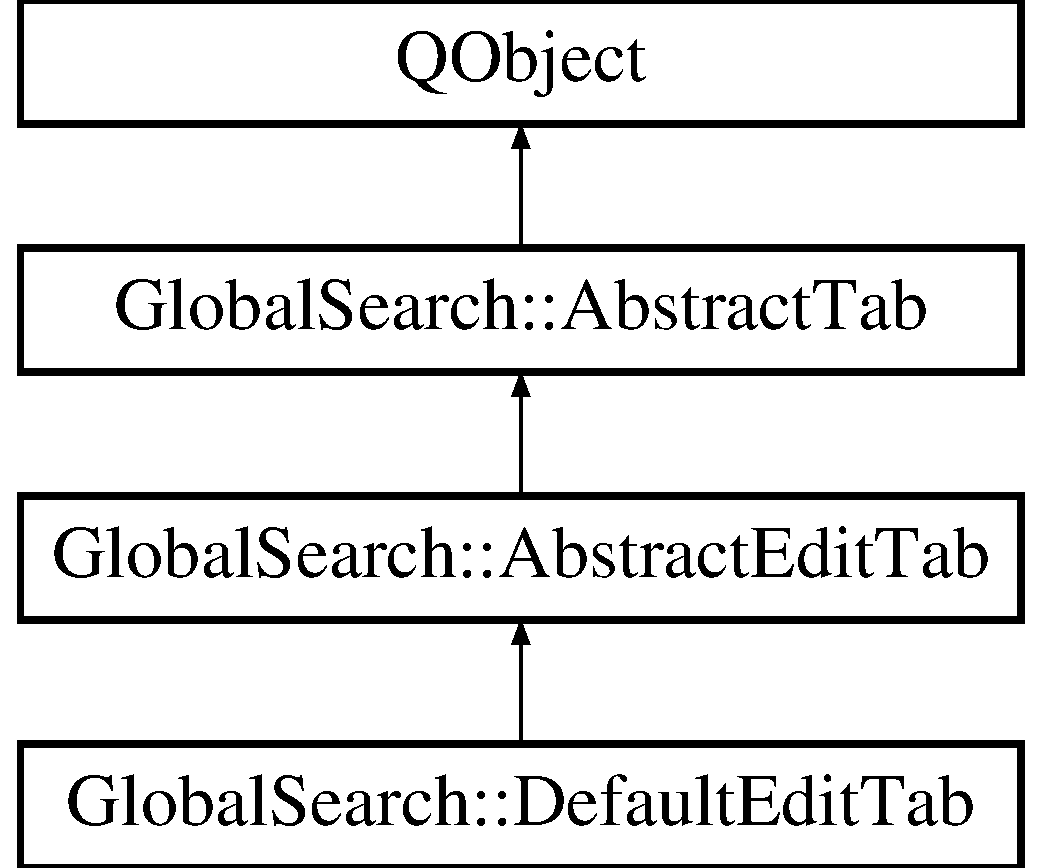
\includegraphics[height=4.000000cm]{classGlobalSearch_1_1AbstractTab}
\end{center}
\end{figure}
\subsection*{Public Slots}
\begin{DoxyCompactItemize}
\item 
virtual void \hyperlink{classGlobalSearch_1_1AbstractTab_a82adaa8137d80906a35beebe92944a3e}{lock\-G\-U\-I} ()
\item 
virtual void \hyperlink{classGlobalSearch_1_1AbstractTab_adc4ad2d0853e7db17a0b147857304cba}{read\-Settings} (const Q\-String \&filename=\char`\"{}\char`\"{})
\item 
virtual void \hyperlink{classGlobalSearch_1_1AbstractTab_a5b09ac7389e664c60ee5ab11a1f8d8fd}{write\-Settings} (const Q\-String \&filename=\char`\"{}\char`\"{})
\item 
virtual void \hyperlink{classGlobalSearch_1_1AbstractTab_a35194ae3ff3b875c1f2e886a69555050}{update\-G\-U\-I} ()
\item 
virtual void \hyperlink{classGlobalSearch_1_1AbstractTab_a63ec89943d1e740fd162877c7cb3679a}{disconnect\-G\-U\-I} ()
\end{DoxyCompactItemize}
\subsection*{Signals}
\begin{DoxyCompactItemize}
\item 
void \hyperlink{classGlobalSearch_1_1AbstractTab_a343c4e401d69ec8364c5a0d53602bb02}{molecule\-Changed} (\hyperlink{classGlobalSearch_1_1Structure}{Global\-Search\-::\-Structure} $\ast$)
\item 
void \hyperlink{classGlobalSearch_1_1AbstractTab_a873c603fd50a66b14d47307aeaaa5fc8}{starting\-Background\-Processing} ()
\item 
void \hyperlink{classGlobalSearch_1_1AbstractTab_a5b06b32887aa1ba75cfcfad24f9c9a86}{finished\-Background\-Processing} ()
\item 
void \hyperlink{classGlobalSearch_1_1AbstractTab_aed63eed75abeb8c0e1e87344225f95cd}{initialized} ()
\end{DoxyCompactItemize}
\subsection*{Public Member Functions}
\begin{DoxyCompactItemize}
\item 
\hyperlink{classGlobalSearch_1_1AbstractTab_aead424f45ea35bc3b8d5d57dc64a9d70}{Abstract\-Tab} (\hyperlink{classGlobalSearch_1_1AbstractDialog}{Abstract\-Dialog} $\ast$parent, \hyperlink{classGlobalSearch_1_1OptBase}{Opt\-Base} $\ast$p)
\item 
virtual \hyperlink{classGlobalSearch_1_1AbstractTab_ab1c9b883cf4fc56d38045028600e20b7}{$\sim$\-Abstract\-Tab} ()
\item 
Q\-Widget $\ast$ \hyperlink{classGlobalSearch_1_1AbstractTab_a2ee691faf240a36dafde7620dc9a9293}{get\-Tab\-Widget} ()
\end{DoxyCompactItemize}
\subsection*{Protected Slots}
\begin{DoxyCompactItemize}
\item 
virtual void \hyperlink{classGlobalSearch_1_1AbstractTab_a70d03cb6f128710bd2af11a7915acad4}{initialize} ()
\item 
void \hyperlink{classGlobalSearch_1_1AbstractTab_a4c6f7ae72bcc7e1eaf06734b7ccb8635}{set\-Busy\-Cursor} ()
\item 
void \hyperlink{classGlobalSearch_1_1AbstractTab_a32efcb7e485b106fc728f39d3174df0e}{clear\-Busy\-Cursor} ()
\end{DoxyCompactItemize}
\subsection*{Protected Attributes}
\begin{DoxyCompactItemize}
\item 
\hypertarget{classGlobalSearch_1_1AbstractTab_a7c461733097abaefd6709de1516b2b6b}{Q\-Widget $\ast$ \hyperlink{classGlobalSearch_1_1AbstractTab_a7c461733097abaefd6709de1516b2b6b}{m\-\_\-tab\-\_\-widget}}\label{classGlobalSearch_1_1AbstractTab_a7c461733097abaefd6709de1516b2b6b}

\begin{DoxyCompactList}\small\item\em The actual widget that will be made into a tab. \end{DoxyCompactList}\item 
\hypertarget{classGlobalSearch_1_1AbstractTab_a1bbcd914bf7dfc64f0c7212719ce8001}{\hyperlink{classGlobalSearch_1_1AbstractDialog}{Abstract\-Dialog} $\ast$ \hyperlink{classGlobalSearch_1_1AbstractTab_a1bbcd914bf7dfc64f0c7212719ce8001}{m\-\_\-dialog}}\label{classGlobalSearch_1_1AbstractTab_a1bbcd914bf7dfc64f0c7212719ce8001}

\begin{DoxyCompactList}\small\item\em A pointer to the parent dialog. \end{DoxyCompactList}\item 
\hypertarget{classGlobalSearch_1_1AbstractTab_a1bf5c32868bc8e6024358078838fb87a}{\hyperlink{classGlobalSearch_1_1OptBase}{Opt\-Base} $\ast$ \hyperlink{classGlobalSearch_1_1AbstractTab_a1bf5c32868bc8e6024358078838fb87a}{m\-\_\-opt}}\label{classGlobalSearch_1_1AbstractTab_a1bf5c32868bc8e6024358078838fb87a}

\begin{DoxyCompactList}\small\item\em A pointer to the associated \hyperlink{classGlobalSearch_1_1OptBase}{Opt\-Base} class. \end{DoxyCompactList}\item 
\hypertarget{classGlobalSearch_1_1AbstractTab_a98d4e176a6385cc5ef29c1436cac1e46}{bool \hyperlink{classGlobalSearch_1_1AbstractTab_a98d4e176a6385cc5ef29c1436cac1e46}{m\-\_\-is\-Initialized}}\label{classGlobalSearch_1_1AbstractTab_a98d4e176a6385cc5ef29c1436cac1e46}

\begin{DoxyCompactList}\small\item\em Set to true once \hyperlink{classGlobalSearch_1_1AbstractTab_aed63eed75abeb8c0e1e87344225f95cd}{initialized()} completes. \end{DoxyCompactList}\end{DoxyCompactItemize}


\subsection{Detailed Description}
The base class for U\-I tabs, preconfigured to work with dialogs derived from \hyperlink{classGlobalSearch_1_1AbstractDialog}{Abstract\-Dialog}. 

\begin{DoxyAuthor}{Author}
David C. Lonie 
\end{DoxyAuthor}


Definition at line 35 of file abstracttab.\-h.



\subsection{Constructor \& Destructor Documentation}
\hypertarget{classGlobalSearch_1_1AbstractTab_aead424f45ea35bc3b8d5d57dc64a9d70}{\index{Global\-Search\-::\-Abstract\-Tab@{Global\-Search\-::\-Abstract\-Tab}!Abstract\-Tab@{Abstract\-Tab}}
\index{Abstract\-Tab@{Abstract\-Tab}!GlobalSearch::AbstractTab@{Global\-Search\-::\-Abstract\-Tab}}
\subsubsection[{Abstract\-Tab}]{\setlength{\rightskip}{0pt plus 5cm}Global\-Search\-::\-Abstract\-Tab\-::\-Abstract\-Tab (
\begin{DoxyParamCaption}
\item[{{\bf Abstract\-Dialog} $\ast$}]{parent, }
\item[{{\bf Opt\-Base} $\ast$}]{p}
\end{DoxyParamCaption}
)\hspace{0.3cm}{\ttfamily [explicit]}}}\label{classGlobalSearch_1_1AbstractTab_aead424f45ea35bc3b8d5d57dc64a9d70}
Constructor

Minimum constructor for derived tab\-: \begin{DoxyVerb}  DerivedTab::DerivedTab(AbstractDialog *parent,
                         OptBase *p) :
    AbstractTab(parent, p)
  {
  ui.setupUi(m_tab_widget);

  initialize();
  }
\end{DoxyVerb}
 

Definition at line 28 of file abstracttab.\-cpp.



References m\-\_\-tab\-\_\-widget.

\hypertarget{classGlobalSearch_1_1AbstractTab_ab1c9b883cf4fc56d38045028600e20b7}{\index{Global\-Search\-::\-Abstract\-Tab@{Global\-Search\-::\-Abstract\-Tab}!$\sim$\-Abstract\-Tab@{$\sim$\-Abstract\-Tab}}
\index{$\sim$\-Abstract\-Tab@{$\sim$\-Abstract\-Tab}!GlobalSearch::AbstractTab@{Global\-Search\-::\-Abstract\-Tab}}
\subsubsection[{$\sim$\-Abstract\-Tab}]{\setlength{\rightskip}{0pt plus 5cm}Global\-Search\-::\-Abstract\-Tab\-::$\sim$\-Abstract\-Tab (
\begin{DoxyParamCaption}
{}
\end{DoxyParamCaption}
)\hspace{0.3cm}{\ttfamily [virtual]}}}\label{classGlobalSearch_1_1AbstractTab_ab1c9b883cf4fc56d38045028600e20b7}
Destructor 

Definition at line 72 of file abstracttab.\-cpp.



\subsection{Member Function Documentation}
\hypertarget{classGlobalSearch_1_1AbstractTab_a32efcb7e485b106fc728f39d3174df0e}{\index{Global\-Search\-::\-Abstract\-Tab@{Global\-Search\-::\-Abstract\-Tab}!clear\-Busy\-Cursor@{clear\-Busy\-Cursor}}
\index{clear\-Busy\-Cursor@{clear\-Busy\-Cursor}!GlobalSearch::AbstractTab@{Global\-Search\-::\-Abstract\-Tab}}
\subsubsection[{clear\-Busy\-Cursor}]{\setlength{\rightskip}{0pt plus 5cm}void Global\-Search\-::\-Abstract\-Tab\-::clear\-Busy\-Cursor (
\begin{DoxyParamCaption}
{}
\end{DoxyParamCaption}
)\hspace{0.3cm}{\ttfamily [protected]}, {\ttfamily [slot]}}}\label{classGlobalSearch_1_1AbstractTab_a32efcb7e485b106fc728f39d3174df0e}
Resets the application's busy cursor. This should not be called directly, instead emit \hyperlink{classGlobalSearch_1_1AbstractTab_a5b06b32887aa1ba75cfcfad24f9c9a86}{finished\-Background\-Processing()}, which is safe to use from a background thread.

\begin{DoxySeeAlso}{See Also}
\hyperlink{classGlobalSearch_1_1AbstractTab_a873c603fd50a66b14d47307aeaaa5fc8}{starting\-Background\-Processing()} 

\hyperlink{classGlobalSearch_1_1AbstractTab_a5b06b32887aa1ba75cfcfad24f9c9a86}{finished\-Background\-Processing()} 
\end{DoxySeeAlso}


Definition at line 84 of file abstracttab.\-cpp.



Referenced by initialize().

\hypertarget{classGlobalSearch_1_1AbstractTab_a63ec89943d1e740fd162877c7cb3679a}{\index{Global\-Search\-::\-Abstract\-Tab@{Global\-Search\-::\-Abstract\-Tab}!disconnect\-G\-U\-I@{disconnect\-G\-U\-I}}
\index{disconnect\-G\-U\-I@{disconnect\-G\-U\-I}!GlobalSearch::AbstractTab@{Global\-Search\-::\-Abstract\-Tab}}
\subsubsection[{disconnect\-G\-U\-I}]{\setlength{\rightskip}{0pt plus 5cm}virtual void Global\-Search\-::\-Abstract\-Tab\-::disconnect\-G\-U\-I (
\begin{DoxyParamCaption}
{}
\end{DoxyParamCaption}
)\hspace{0.3cm}{\ttfamily [inline]}, {\ttfamily [virtual]}, {\ttfamily [slot]}}}\label{classGlobalSearch_1_1AbstractTab_a63ec89943d1e740fd162877c7cb3679a}
Used during benchmarking to disable any G\-U\-I update connections. 

Definition at line 104 of file abstracttab.\-h.



Referenced by initialize().

\hypertarget{classGlobalSearch_1_1AbstractTab_a5b06b32887aa1ba75cfcfad24f9c9a86}{\index{Global\-Search\-::\-Abstract\-Tab@{Global\-Search\-::\-Abstract\-Tab}!finished\-Background\-Processing@{finished\-Background\-Processing}}
\index{finished\-Background\-Processing@{finished\-Background\-Processing}!GlobalSearch::AbstractTab@{Global\-Search\-::\-Abstract\-Tab}}
\subsubsection[{finished\-Background\-Processing}]{\setlength{\rightskip}{0pt plus 5cm}void Global\-Search\-::\-Abstract\-Tab\-::finished\-Background\-Processing (
\begin{DoxyParamCaption}
{}
\end{DoxyParamCaption}
)\hspace{0.3cm}{\ttfamily [signal]}}}\label{classGlobalSearch_1_1AbstractTab_a5b06b32887aa1ba75cfcfad24f9c9a86}
Emit this signal after user-\/requested processing has completed. This will reset the busy cursor in the application. 

Referenced by initialize().

\hypertarget{classGlobalSearch_1_1AbstractTab_a2ee691faf240a36dafde7620dc9a9293}{\index{Global\-Search\-::\-Abstract\-Tab@{Global\-Search\-::\-Abstract\-Tab}!get\-Tab\-Widget@{get\-Tab\-Widget}}
\index{get\-Tab\-Widget@{get\-Tab\-Widget}!GlobalSearch::AbstractTab@{Global\-Search\-::\-Abstract\-Tab}}
\subsubsection[{get\-Tab\-Widget}]{\setlength{\rightskip}{0pt plus 5cm}Q\-Widget$\ast$ Global\-Search\-::\-Abstract\-Tab\-::get\-Tab\-Widget (
\begin{DoxyParamCaption}
{}
\end{DoxyParamCaption}
)\hspace{0.3cm}{\ttfamily [inline]}}}\label{classGlobalSearch_1_1AbstractTab_a2ee691faf240a36dafde7620dc9a9293}
\begin{DoxyReturn}{Returns}
The widget for this tab. 
\end{DoxyReturn}


Definition at line 66 of file abstracttab.\-h.



References m\-\_\-tab\-\_\-widget.

\hypertarget{classGlobalSearch_1_1AbstractTab_a70d03cb6f128710bd2af11a7915acad4}{\index{Global\-Search\-::\-Abstract\-Tab@{Global\-Search\-::\-Abstract\-Tab}!initialize@{initialize}}
\index{initialize@{initialize}!GlobalSearch::AbstractTab@{Global\-Search\-::\-Abstract\-Tab}}
\subsubsection[{initialize}]{\setlength{\rightskip}{0pt plus 5cm}void Global\-Search\-::\-Abstract\-Tab\-::initialize (
\begin{DoxyParamCaption}
{}
\end{DoxyParamCaption}
)\hspace{0.3cm}{\ttfamily [protected]}, {\ttfamily [virtual]}, {\ttfamily [slot]}}}\label{classGlobalSearch_1_1AbstractTab_a70d03cb6f128710bd2af11a7915acad4}
Create some default connections between the main dialog and this tab. 

Definition at line 38 of file abstracttab.\-cpp.



References clear\-Busy\-Cursor(), disconnect\-G\-U\-I(), finished\-Background\-Processing(), initialized(), lock\-G\-U\-I(), m\-\_\-dialog, m\-\_\-is\-Initialized, molecule\-Changed(), read\-Settings(), set\-Busy\-Cursor(), starting\-Background\-Processing(), update\-G\-U\-I(), and write\-Settings().



Referenced by Global\-Search\-::\-Abstract\-Edit\-Tab\-::initialize().

\hypertarget{classGlobalSearch_1_1AbstractTab_aed63eed75abeb8c0e1e87344225f95cd}{\index{Global\-Search\-::\-Abstract\-Tab@{Global\-Search\-::\-Abstract\-Tab}!initialized@{initialized}}
\index{initialized@{initialized}!GlobalSearch::AbstractTab@{Global\-Search\-::\-Abstract\-Tab}}
\subsubsection[{initialized}]{\setlength{\rightskip}{0pt plus 5cm}void Global\-Search\-::\-Abstract\-Tab\-::initialized (
\begin{DoxyParamCaption}
{}
\end{DoxyParamCaption}
)\hspace{0.3cm}{\ttfamily [signal]}}}\label{classGlobalSearch_1_1AbstractTab_aed63eed75abeb8c0e1e87344225f95cd}
Emitted when initialize completes 

Referenced by initialize().

\hypertarget{classGlobalSearch_1_1AbstractTab_a82adaa8137d80906a35beebe92944a3e}{\index{Global\-Search\-::\-Abstract\-Tab@{Global\-Search\-::\-Abstract\-Tab}!lock\-G\-U\-I@{lock\-G\-U\-I}}
\index{lock\-G\-U\-I@{lock\-G\-U\-I}!GlobalSearch::AbstractTab@{Global\-Search\-::\-Abstract\-Tab}}
\subsubsection[{lock\-G\-U\-I}]{\setlength{\rightskip}{0pt plus 5cm}virtual void Global\-Search\-::\-Abstract\-Tab\-::lock\-G\-U\-I (
\begin{DoxyParamCaption}
{}
\end{DoxyParamCaption}
)\hspace{0.3cm}{\ttfamily [inline]}, {\ttfamily [virtual]}, {\ttfamily [slot]}}}\label{classGlobalSearch_1_1AbstractTab_a82adaa8137d80906a35beebe92944a3e}
Disable portions of the G\-U\-I that shouldn't be modified after the search has started. 

Definition at line 73 of file abstracttab.\-h.



Referenced by initialize().

\hypertarget{classGlobalSearch_1_1AbstractTab_a343c4e401d69ec8364c5a0d53602bb02}{\index{Global\-Search\-::\-Abstract\-Tab@{Global\-Search\-::\-Abstract\-Tab}!molecule\-Changed@{molecule\-Changed}}
\index{molecule\-Changed@{molecule\-Changed}!GlobalSearch::AbstractTab@{Global\-Search\-::\-Abstract\-Tab}}
\subsubsection[{molecule\-Changed}]{\setlength{\rightskip}{0pt plus 5cm}void Global\-Search\-::\-Abstract\-Tab\-::molecule\-Changed (
\begin{DoxyParamCaption}
\item[{{\bf Global\-Search\-::\-Structure} $\ast$}]{}
\end{DoxyParamCaption}
)\hspace{0.3cm}{\ttfamily [signal]}}}\label{classGlobalSearch_1_1AbstractTab_a343c4e401d69ec8364c5a0d53602bb02}
Emit to update the molecule displayed in the Avogadro G\-L\-Widget 

Referenced by initialize().

\hypertarget{classGlobalSearch_1_1AbstractTab_adc4ad2d0853e7db17a0b147857304cba}{\index{Global\-Search\-::\-Abstract\-Tab@{Global\-Search\-::\-Abstract\-Tab}!read\-Settings@{read\-Settings}}
\index{read\-Settings@{read\-Settings}!GlobalSearch::AbstractTab@{Global\-Search\-::\-Abstract\-Tab}}
\subsubsection[{read\-Settings}]{\setlength{\rightskip}{0pt plus 5cm}virtual void Global\-Search\-::\-Abstract\-Tab\-::read\-Settings (
\begin{DoxyParamCaption}
\item[{const Q\-String \&}]{filename = {\ttfamily \char`\"{}\char`\"{}}}
\end{DoxyParamCaption}
)\hspace{0.3cm}{\ttfamily [inline]}, {\ttfamily [virtual]}, {\ttfamily [slot]}}}\label{classGlobalSearch_1_1AbstractTab_adc4ad2d0853e7db17a0b147857304cba}
Load any parameters that this tab is responible for here. \begin{DoxyNote}{Note}
In most cases, this shouldn't be called directly, but rather call the same function in the parent dialog class. 
\end{DoxyNote}

\begin{DoxyParams}{Parameters}
{\em filename} & If specified, read from given file. Otherwise read from system config file. \\
\hline
\end{DoxyParams}


Definition at line 82 of file abstracttab.\-h.



Referenced by initialize(), and Global\-Search\-::\-Abstract\-Edit\-Tab\-::load\-Scheme().

\hypertarget{classGlobalSearch_1_1AbstractTab_a4c6f7ae72bcc7e1eaf06734b7ccb8635}{\index{Global\-Search\-::\-Abstract\-Tab@{Global\-Search\-::\-Abstract\-Tab}!set\-Busy\-Cursor@{set\-Busy\-Cursor}}
\index{set\-Busy\-Cursor@{set\-Busy\-Cursor}!GlobalSearch::AbstractTab@{Global\-Search\-::\-Abstract\-Tab}}
\subsubsection[{set\-Busy\-Cursor}]{\setlength{\rightskip}{0pt plus 5cm}void Global\-Search\-::\-Abstract\-Tab\-::set\-Busy\-Cursor (
\begin{DoxyParamCaption}
{}
\end{DoxyParamCaption}
)\hspace{0.3cm}{\ttfamily [protected]}, {\ttfamily [slot]}}}\label{classGlobalSearch_1_1AbstractTab_a4c6f7ae72bcc7e1eaf06734b7ccb8635}
Sets the application's busy cursor. This should not be called directly, instead emit \hyperlink{classGlobalSearch_1_1AbstractTab_a873c603fd50a66b14d47307aeaaa5fc8}{starting\-Background\-Processing()}, which is safe to use from a background thread.

\begin{DoxySeeAlso}{See Also}
\hyperlink{classGlobalSearch_1_1AbstractTab_a873c603fd50a66b14d47307aeaaa5fc8}{starting\-Background\-Processing()} 

\hyperlink{classGlobalSearch_1_1AbstractTab_a5b06b32887aa1ba75cfcfad24f9c9a86}{finished\-Background\-Processing()} 
\end{DoxySeeAlso}


Definition at line 76 of file abstracttab.\-cpp.



Referenced by initialize().

\hypertarget{classGlobalSearch_1_1AbstractTab_a873c603fd50a66b14d47307aeaaa5fc8}{\index{Global\-Search\-::\-Abstract\-Tab@{Global\-Search\-::\-Abstract\-Tab}!starting\-Background\-Processing@{starting\-Background\-Processing}}
\index{starting\-Background\-Processing@{starting\-Background\-Processing}!GlobalSearch::AbstractTab@{Global\-Search\-::\-Abstract\-Tab}}
\subsubsection[{starting\-Background\-Processing}]{\setlength{\rightskip}{0pt plus 5cm}void Global\-Search\-::\-Abstract\-Tab\-::starting\-Background\-Processing (
\begin{DoxyParamCaption}
{}
\end{DoxyParamCaption}
)\hspace{0.3cm}{\ttfamily [signal]}}}\label{classGlobalSearch_1_1AbstractTab_a873c603fd50a66b14d47307aeaaa5fc8}
Emit this signal before beginning user-\/requested processing. This will set the busy cursor in the application. 

Referenced by initialize().

\hypertarget{classGlobalSearch_1_1AbstractTab_a35194ae3ff3b875c1f2e886a69555050}{\index{Global\-Search\-::\-Abstract\-Tab@{Global\-Search\-::\-Abstract\-Tab}!update\-G\-U\-I@{update\-G\-U\-I}}
\index{update\-G\-U\-I@{update\-G\-U\-I}!GlobalSearch::AbstractTab@{Global\-Search\-::\-Abstract\-Tab}}
\subsubsection[{update\-G\-U\-I}]{\setlength{\rightskip}{0pt plus 5cm}virtual void Global\-Search\-::\-Abstract\-Tab\-::update\-G\-U\-I (
\begin{DoxyParamCaption}
{}
\end{DoxyParamCaption}
)\hspace{0.3cm}{\ttfamily [inline]}, {\ttfamily [virtual]}, {\ttfamily [slot]}}}\label{classGlobalSearch_1_1AbstractTab_a35194ae3ff3b875c1f2e886a69555050}
Set any G\-U\-I elements from information in internal data structures. 

Definition at line 99 of file abstracttab.\-h.



Referenced by initialize().

\hypertarget{classGlobalSearch_1_1AbstractTab_a5b09ac7389e664c60ee5ab11a1f8d8fd}{\index{Global\-Search\-::\-Abstract\-Tab@{Global\-Search\-::\-Abstract\-Tab}!write\-Settings@{write\-Settings}}
\index{write\-Settings@{write\-Settings}!GlobalSearch::AbstractTab@{Global\-Search\-::\-Abstract\-Tab}}
\subsubsection[{write\-Settings}]{\setlength{\rightskip}{0pt plus 5cm}virtual void Global\-Search\-::\-Abstract\-Tab\-::write\-Settings (
\begin{DoxyParamCaption}
\item[{const Q\-String \&}]{filename = {\ttfamily \char`\"{}\char`\"{}}}
\end{DoxyParamCaption}
)\hspace{0.3cm}{\ttfamily [inline]}, {\ttfamily [virtual]}, {\ttfamily [slot]}}}\label{classGlobalSearch_1_1AbstractTab_a5b09ac7389e664c60ee5ab11a1f8d8fd}
Save any parameters that this tab is responible for here. \begin{DoxyNote}{Note}
In most cases, this shouldn't be called directly, but rather call the same function in the parent dialog class. 
\end{DoxyNote}

\begin{DoxyParams}{Parameters}
{\em filename} & If specified, write to given file. Otherwise write to system config file. \\
\hline
\end{DoxyParams}


Definition at line 92 of file abstracttab.\-h.



Referenced by initialize(), and Global\-Search\-::\-Abstract\-Edit\-Tab\-::save\-Scheme().



The documentation for this class was generated from the following files\-:\begin{DoxyCompactItemize}
\item 
src/globalsearch/ui/abstracttab.\-h\item 
src/globalsearch/ui/abstracttab.\-cpp\end{DoxyCompactItemize}

\hypertarget{classGlobalSearch_1_1DefaultEditTab}{}\section{Global\+Search\+:\+:Default\+Edit\+Tab Class Reference}
\label{classGlobalSearch_1_1DefaultEditTab}\index{Global\+Search\+::\+Default\+Edit\+Tab@{Global\+Search\+::\+Default\+Edit\+Tab}}


Default implementation of a template editor tab.  




{\ttfamily \#include $<$globalsearch/defaultedittab.\+h$>$}

Inheritance diagram for Global\+Search\+:\+:Default\+Edit\+Tab\+:\begin{figure}[H]
\begin{center}
\leavevmode
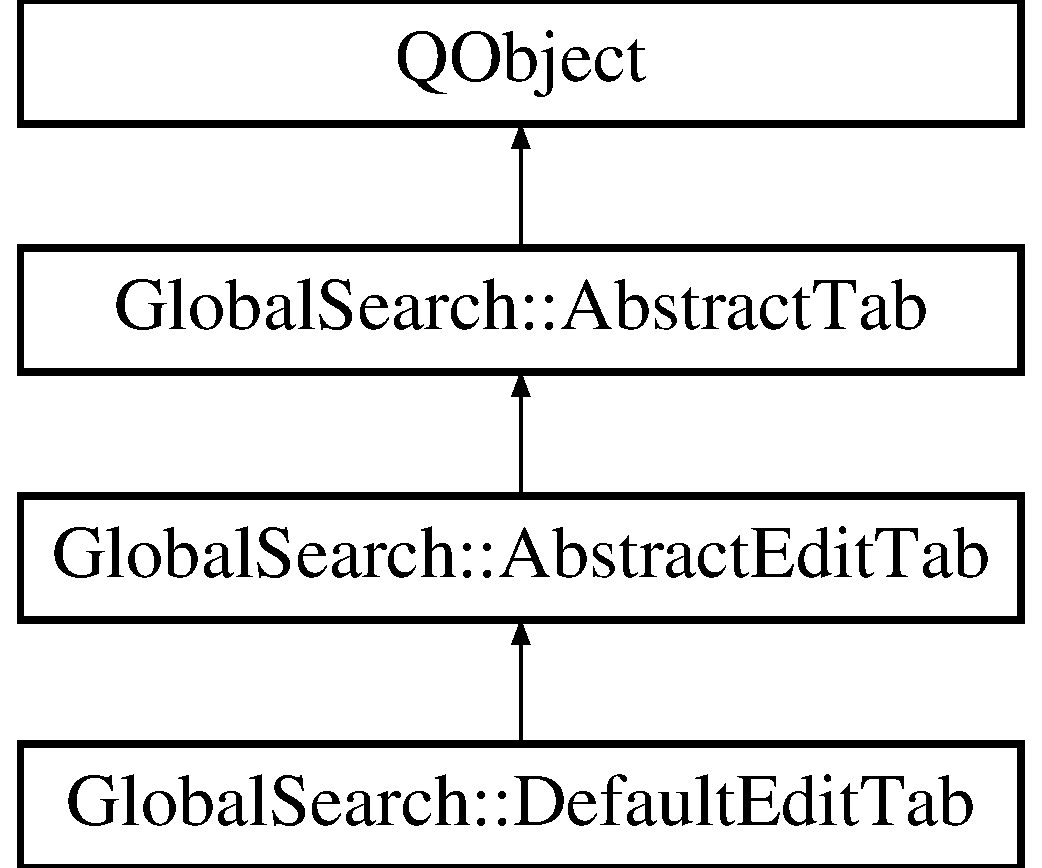
\includegraphics[height=4.000000cm]{classGlobalSearch_1_1DefaultEditTab}
\end{center}
\end{figure}
\subsection*{Public Member Functions}
\begin{DoxyCompactItemize}
\item 
\hyperlink{classGlobalSearch_1_1DefaultEditTab_ae511483de60e194bcf2e82e931da541d}{Default\+Edit\+Tab} (\hyperlink{classGlobalSearch_1_1AbstractDialog}{Abstract\+Dialog} $\ast$dialog, \hyperlink{classGlobalSearch_1_1OptBase}{Opt\+Base} $\ast$opt)
\item 
virtual \hyperlink{classGlobalSearch_1_1DefaultEditTab_ab2b458010ec73753f0e00b568af00d0b}{$\sim$\+Default\+Edit\+Tab} ()
\end{DoxyCompactItemize}
\subsection*{Protected Slots}
\begin{DoxyCompactItemize}
\item 
virtual void \hyperlink{classGlobalSearch_1_1DefaultEditTab_aabb8111d57852154b366640b728baabb}{initialize} ()
\end{DoxyCompactItemize}
\subsection*{Additional Inherited Members}


\subsection{Detailed Description}
Default implementation of a template editor tab. 

\begin{DoxyAuthor}{Author}
David C. Lonie 
\end{DoxyAuthor}


Definition at line 37 of file defaultedittab.\+h.



\subsection{Constructor \& Destructor Documentation}
\hypertarget{classGlobalSearch_1_1DefaultEditTab_ae511483de60e194bcf2e82e931da541d}{}\index{Global\+Search\+::\+Default\+Edit\+Tab@{Global\+Search\+::\+Default\+Edit\+Tab}!Default\+Edit\+Tab@{Default\+Edit\+Tab}}
\index{Default\+Edit\+Tab@{Default\+Edit\+Tab}!Global\+Search\+::\+Default\+Edit\+Tab@{Global\+Search\+::\+Default\+Edit\+Tab}}
\subsubsection[{Default\+Edit\+Tab}]{\setlength{\rightskip}{0pt plus 5cm}Global\+Search\+::\+Default\+Edit\+Tab\+::\+Default\+Edit\+Tab (
\begin{DoxyParamCaption}
\item[{{\bf Abstract\+Dialog} $\ast$}]{dialog, }
\item[{{\bf Opt\+Base} $\ast$}]{opt}
\end{DoxyParamCaption}
)\hspace{0.3cm}{\ttfamily [explicit]}}\label{classGlobalSearch_1_1DefaultEditTab_ae511483de60e194bcf2e82e931da541d}
Constructor


\begin{DoxyParams}{Parameters}
{\em dialog} & Parent \hyperlink{classGlobalSearch_1_1AbstractDialog}{Abstract\+Dialog} \\
\hline
{\em opt} & Associated \hyperlink{classGlobalSearch_1_1OptBase}{Opt\+Base} \\
\hline
\end{DoxyParams}


Definition at line 23 of file defaultedittab.\+cpp.



References Global\+Search\+::\+Abstract\+Tab\+::m\+\_\+tab\+\_\+widget, Global\+Search\+::\+Abstract\+Edit\+Tab\+::ui\+\_\+combo\+\_\+optimizers, Global\+Search\+::\+Abstract\+Edit\+Tab\+::ui\+\_\+combo\+\_\+queue\+Interfaces, Global\+Search\+::\+Abstract\+Edit\+Tab\+::ui\+\_\+combo\+\_\+templates, Global\+Search\+::\+Abstract\+Edit\+Tab\+::ui\+\_\+edit\+\_\+edit, Global\+Search\+::\+Abstract\+Edit\+Tab\+::ui\+\_\+edit\+\_\+user1, Global\+Search\+::\+Abstract\+Edit\+Tab\+::ui\+\_\+edit\+\_\+user2, Global\+Search\+::\+Abstract\+Edit\+Tab\+::ui\+\_\+edit\+\_\+user3, Global\+Search\+::\+Abstract\+Edit\+Tab\+::ui\+\_\+edit\+\_\+user4, Global\+Search\+::\+Abstract\+Edit\+Tab\+::ui\+\_\+list\+\_\+edit, Global\+Search\+::\+Abstract\+Edit\+Tab\+::ui\+\_\+list\+\_\+opt\+Step, Global\+Search\+::\+Abstract\+Edit\+Tab\+::ui\+\_\+push\+\_\+add, Global\+Search\+::\+Abstract\+Edit\+Tab\+::ui\+\_\+push\+\_\+help, Global\+Search\+::\+Abstract\+Edit\+Tab\+::ui\+\_\+push\+\_\+load\+Scheme, Global\+Search\+::\+Abstract\+Edit\+Tab\+::ui\+\_\+push\+\_\+optimizer\+Config, Global\+Search\+::\+Abstract\+Edit\+Tab\+::ui\+\_\+push\+\_\+queue\+Interface\+Config, Global\+Search\+::\+Abstract\+Edit\+Tab\+::ui\+\_\+push\+\_\+remove, and Global\+Search\+::\+Abstract\+Edit\+Tab\+::ui\+\_\+push\+\_\+save\+Scheme.

\hypertarget{classGlobalSearch_1_1DefaultEditTab_ab2b458010ec73753f0e00b568af00d0b}{}\index{Global\+Search\+::\+Default\+Edit\+Tab@{Global\+Search\+::\+Default\+Edit\+Tab}!````~Default\+Edit\+Tab@{$\sim$\+Default\+Edit\+Tab}}
\index{````~Default\+Edit\+Tab@{$\sim$\+Default\+Edit\+Tab}!Global\+Search\+::\+Default\+Edit\+Tab@{Global\+Search\+::\+Default\+Edit\+Tab}}
\subsubsection[{$\sim$\+Default\+Edit\+Tab}]{\setlength{\rightskip}{0pt plus 5cm}Global\+Search\+::\+Default\+Edit\+Tab\+::$\sim$\+Default\+Edit\+Tab (
\begin{DoxyParamCaption}
{}
\end{DoxyParamCaption}
)\hspace{0.3cm}{\ttfamily [virtual]}}\label{classGlobalSearch_1_1DefaultEditTab_ab2b458010ec73753f0e00b568af00d0b}
Destructor 

Definition at line 50 of file defaultedittab.\+cpp.



\subsection{Member Function Documentation}
\hypertarget{classGlobalSearch_1_1DefaultEditTab_aabb8111d57852154b366640b728baabb}{}\index{Global\+Search\+::\+Default\+Edit\+Tab@{Global\+Search\+::\+Default\+Edit\+Tab}!initialize@{initialize}}
\index{initialize@{initialize}!Global\+Search\+::\+Default\+Edit\+Tab@{Global\+Search\+::\+Default\+Edit\+Tab}}
\subsubsection[{initialize}]{\setlength{\rightskip}{0pt plus 5cm}void Global\+Search\+::\+Default\+Edit\+Tab\+::initialize (
\begin{DoxyParamCaption}
{}
\end{DoxyParamCaption}
)\hspace{0.3cm}{\ttfamily [protected]}, {\ttfamily [virtual]}, {\ttfamily [slot]}}\label{classGlobalSearch_1_1DefaultEditTab_aabb8111d57852154b366640b728baabb}
Set up the G\+U\+I pointers and call \hyperlink{classGlobalSearch_1_1AbstractEditTab_afb9fd8fbcf71d7287a8117ce4d75a00b}{Abstract\+Edit\+Tab\+::initialize()} 

Definition at line 55 of file defaultedittab.\+cpp.



References Global\+Search\+::\+Abstract\+Edit\+Tab\+::initialize().



The documentation for this class was generated from the following files\+:\begin{DoxyCompactItemize}
\item 
src/globalsearch/ui/defaultedittab.\+h\item 
src/globalsearch/ui/defaultedittab.\+cpp\end{DoxyCompactItemize}

\hypertarget{classGlobalSearch_1_1GSRandom}{}\subsection{Global\+Search\+:\+:G\+S\+Random Class Reference}
\label{classGlobalSearch_1_1GSRandom}\index{Global\+Search\+::\+G\+S\+Random@{Global\+Search\+::\+G\+S\+Random}}


This class implements a thread-\/safe, cross-\/platform singleton random number generator.  




{\ttfamily \#include $<$globalsearch/random.\+h$>$}

\subsubsection*{Public Member Functions}
\begin{DoxyCompactItemize}
\item 
double \hyperlink{classGlobalSearch_1_1GSRandom_ae648223ac2769459d66f446ac862955e}{get\+Random\+Double} ()
\item 
unsigned int \hyperlink{classGlobalSearch_1_1GSRandom_a225a2c9598d7d6636afecacdd7750228}{get\+Random\+U\+Int} ()
\end{DoxyCompactItemize}
\subsubsection*{Static Public Member Functions}
\begin{DoxyCompactItemize}
\item 
static \hyperlink{classGlobalSearch_1_1GSRandom}{G\+S\+Random} $\ast$ \hyperlink{classGlobalSearch_1_1GSRandom_a19c0a95c0f92f3ffedfbcb4e4f15a782}{instance} ()
\end{DoxyCompactItemize}
\subsubsection*{Protected Member Functions}
\begin{DoxyCompactItemize}
\item 
\hypertarget{classGlobalSearch_1_1GSRandom_a87c1478f68605a85be05376799898185}{}\hyperlink{classGlobalSearch_1_1GSRandom_a87c1478f68605a85be05376799898185}{G\+S\+Random} ()\label{classGlobalSearch_1_1GSRandom_a87c1478f68605a85be05376799898185}

\begin{DoxyCompactList}\small\item\em Constructor. \end{DoxyCompactList}\item 
\hypertarget{classGlobalSearch_1_1GSRandom_a43fb2fb498f272c8150e59e58ca8ce37}{}\hyperlink{classGlobalSearch_1_1GSRandom_a43fb2fb498f272c8150e59e58ca8ce37}{G\+S\+Random} (const \hyperlink{classGlobalSearch_1_1GSRandom}{G\+S\+Random} \&)\label{classGlobalSearch_1_1GSRandom_a43fb2fb498f272c8150e59e58ca8ce37}

\begin{DoxyCompactList}\small\item\em Disabled copy constructor. \end{DoxyCompactList}\item 
\hypertarget{classGlobalSearch_1_1GSRandom_ac4d2afd7e581d4d3daa9def13f34f11a}{}\hyperlink{classGlobalSearch_1_1GSRandom}{G\+S\+Random} \& \hyperlink{classGlobalSearch_1_1GSRandom_ac4d2afd7e581d4d3daa9def13f34f11a}{operator=} (const \hyperlink{classGlobalSearch_1_1GSRandom}{G\+S\+Random} \&)\label{classGlobalSearch_1_1GSRandom_ac4d2afd7e581d4d3daa9def13f34f11a}

\begin{DoxyCompactList}\small\item\em Disabled assignment operator. \end{DoxyCompactList}\end{DoxyCompactItemize}


\subsubsection{Detailed Description}
This class implements a thread-\/safe, cross-\/platform singleton random number generator. 

Direct use of this class is discouraged. Rather, use the R\+A\+N\+D\+D\+O\+U\+B\+L\+E(), etc macros in \hyperlink{macros_8h_source}{globalsearch/macros.\+h}.

\begin{DoxyAuthor}{Author}
David C. Lonie 
\end{DoxyAuthor}


Definition at line 32 of file random.\+h.



\subsubsection{Member Function Documentation}
\hypertarget{classGlobalSearch_1_1GSRandom_ae648223ac2769459d66f446ac862955e}{}\index{Global\+Search\+::\+G\+S\+Random@{Global\+Search\+::\+G\+S\+Random}!get\+Random\+Double@{get\+Random\+Double}}
\index{get\+Random\+Double@{get\+Random\+Double}!Global\+Search\+::\+G\+S\+Random@{Global\+Search\+::\+G\+S\+Random}}
\paragraph[{get\+Random\+Double}]{\setlength{\rightskip}{0pt plus 5cm}double Global\+Search\+::\+G\+S\+Random\+::get\+Random\+Double (
\begin{DoxyParamCaption}
{}
\end{DoxyParamCaption}
)}\label{classGlobalSearch_1_1GSRandom_ae648223ac2769459d66f446ac862955e}
\begin{DoxyReturn}{Returns}
a random floating point number between zero and one 
\end{DoxyReturn}


Definition at line 67 of file random.\+cpp.

\hypertarget{classGlobalSearch_1_1GSRandom_a225a2c9598d7d6636afecacdd7750228}{}\index{Global\+Search\+::\+G\+S\+Random@{Global\+Search\+::\+G\+S\+Random}!get\+Random\+U\+Int@{get\+Random\+U\+Int}}
\index{get\+Random\+U\+Int@{get\+Random\+U\+Int}!Global\+Search\+::\+G\+S\+Random@{Global\+Search\+::\+G\+S\+Random}}
\paragraph[{get\+Random\+U\+Int}]{\setlength{\rightskip}{0pt plus 5cm}unsigned int Global\+Search\+::\+G\+S\+Random\+::get\+Random\+U\+Int (
\begin{DoxyParamCaption}
{}
\end{DoxyParamCaption}
)}\label{classGlobalSearch_1_1GSRandom_a225a2c9598d7d6636afecacdd7750228}
\begin{DoxyReturn}{Returns}
a random unsigned integer 
\end{DoxyReturn}


Definition at line 76 of file random.\+cpp.

\hypertarget{classGlobalSearch_1_1GSRandom_a19c0a95c0f92f3ffedfbcb4e4f15a782}{}\index{Global\+Search\+::\+G\+S\+Random@{Global\+Search\+::\+G\+S\+Random}!instance@{instance}}
\index{instance@{instance}!Global\+Search\+::\+G\+S\+Random@{Global\+Search\+::\+G\+S\+Random}}
\paragraph[{instance}]{\setlength{\rightskip}{0pt plus 5cm}{\bf G\+S\+Random} $\ast$ Global\+Search\+::\+G\+S\+Random\+::instance (
\begin{DoxyParamCaption}
{}
\end{DoxyParamCaption}
)\hspace{0.3cm}{\ttfamily [static]}}\label{classGlobalSearch_1_1GSRandom_a19c0a95c0f92f3ffedfbcb4e4f15a782}
\begin{DoxyReturn}{Returns}
the global \hyperlink{classGlobalSearch_1_1GSRandom}{G\+S\+Random} instance 
\end{DoxyReturn}


Definition at line 50 of file random.\+cpp.



References G\+S\+Random().



The documentation for this class was generated from the following files\+:\begin{DoxyCompactItemize}
\item 
src/globalsearch/random.\+h\item 
src/globalsearch/random.\+cpp\end{DoxyCompactItemize}

\hypertarget{classGlobalSearch_1_1LocalQueueInterface}{}\section{Global\+Search\+:\+:Local\+Queue\+Interface Class Reference}
\label{classGlobalSearch_1_1LocalQueueInterface}\index{Global\+Search\+::\+Local\+Queue\+Interface@{Global\+Search\+::\+Local\+Queue\+Interface}}


Interface for running jobs locally.  




{\ttfamily \#include $<$globalsearch/local.\+h$>$}

Inheritance diagram for Global\+Search\+:\+:Local\+Queue\+Interface\+:\begin{figure}[H]
\begin{center}
\leavevmode
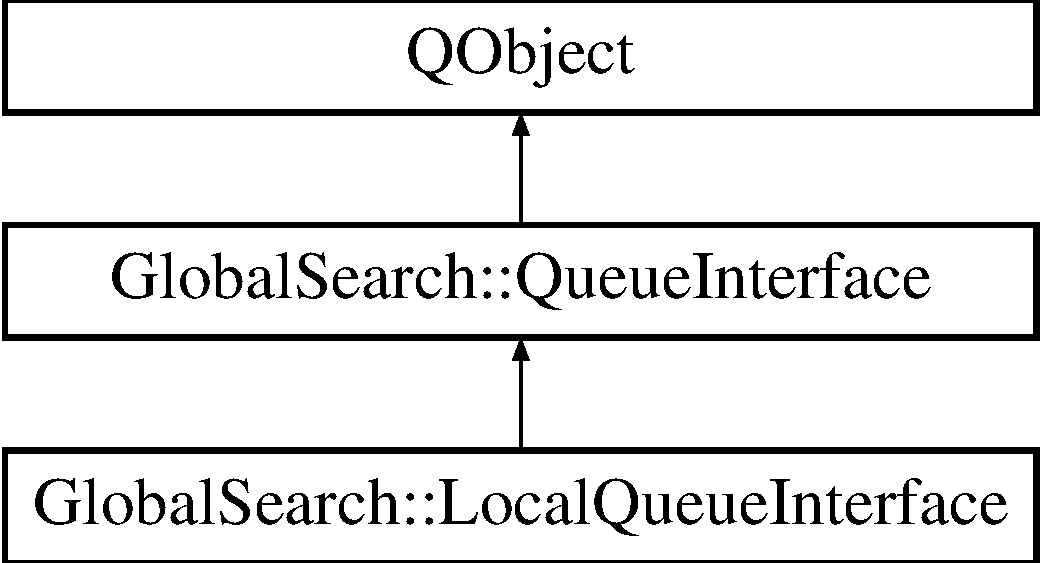
\includegraphics[height=3.000000cm]{classGlobalSearch_1_1LocalQueueInterface}
\end{center}
\end{figure}
\subsection*{Public Slots}
\begin{DoxyCompactItemize}
\item 
virtual bool \hyperlink{classGlobalSearch_1_1LocalQueueInterface_a68b017d4ee519055fc22dcb486ec2d45}{write\+Files} (\hyperlink{classGlobalSearch_1_1Structure}{Structure} $\ast$s, const Q\+Hash$<$ Q\+String, Q\+String $>$ \&files) const 
\item 
virtual bool \hyperlink{classGlobalSearch_1_1LocalQueueInterface_a5dae655b3316d9443ca5865a65b8d9f4}{start\+Job} (\hyperlink{classGlobalSearch_1_1Structure}{Structure} $\ast$s)
\item 
virtual bool \hyperlink{classGlobalSearch_1_1LocalQueueInterface_abd9adf1468347b0bdcc4f1f8c3676c1a}{stop\+Job} (\hyperlink{classGlobalSearch_1_1Structure}{Structure} $\ast$s)
\item 
virtual \hyperlink{classGlobalSearch_1_1QueueInterface_a08dcf06d1b99f6333472470490ca9a6d}{Queue\+Interface\+::\+Queue\+Status} \hyperlink{classGlobalSearch_1_1LocalQueueInterface_a1a6177bcf15d3df5dd744ca096cab86d}{get\+Status} (\hyperlink{classGlobalSearch_1_1Structure}{Structure} $\ast$s) const 
\item 
virtual bool \hyperlink{classGlobalSearch_1_1LocalQueueInterface_aec8ffad280b7e550d90529624c3b50fe}{prepare\+For\+Structure\+Update} (\hyperlink{classGlobalSearch_1_1Structure}{Structure} $\ast$s) const 
\item 
virtual bool \hyperlink{classGlobalSearch_1_1LocalQueueInterface_a7dfd8f70a313746a2651b405651d5c6c}{check\+If\+File\+Exists} (\hyperlink{classGlobalSearch_1_1Structure}{Structure} $\ast$s, const Q\+String \&filename, bool $\ast$exists)
\item 
virtual bool \hyperlink{classGlobalSearch_1_1LocalQueueInterface_ae0b1b95c62405c79b41604b7a4794a0d}{fetch\+File} (\hyperlink{classGlobalSearch_1_1Structure}{Structure} $\ast$s, const Q\+String \&filename, Q\+String $\ast$contents) const 
\item 
virtual bool \hyperlink{classGlobalSearch_1_1LocalQueueInterface_a948f5d6109f3fd3dff74799bb7573363}{grep\+File} (\hyperlink{classGlobalSearch_1_1Structure}{Structure} $\ast$s, const Q\+String \&match\+Text, const Q\+String \&filename, Q\+String\+List $\ast$matches=0, int $\ast$exitcode=0, const bool case\+Sensitive=true) const 
\item 
virtual Q\+Dialog $\ast$ \hyperlink{group__dialog_ga4bd87bf2050209a72d1a35c824e515da}{dialog} ()
\end{DoxyCompactItemize}
\subsection*{Public Member Functions}
\begin{DoxyCompactItemize}
\item 
\hyperlink{classGlobalSearch_1_1LocalQueueInterface_ae1188c7950216c209249923050410489}{Local\+Queue\+Interface} (\hyperlink{classGlobalSearch_1_1OptBase}{Opt\+Base} $\ast$parent, const Q\+String \&setting\+File=\char`\"{}\char`\"{})
\item 
virtual \hyperlink{classGlobalSearch_1_1LocalQueueInterface_a1749a7451caa140ecd6cc244a5117f99}{$\sim$\+Local\+Queue\+Interface} ()
\item 
virtual bool \hyperlink{classGlobalSearch_1_1LocalQueueInterface_ab414f1b5b47610e45fece054512566ed}{is\+Ready\+To\+Search} (Q\+String $\ast$err)
\end{DoxyCompactItemize}
\subsection*{Protected Attributes}
\begin{DoxyCompactItemize}
\item 
Q\+Hash$<$ unsigned long, Local\+Queue\+Process $\ast$ $>$ \hyperlink{classGlobalSearch_1_1LocalQueueInterface_a7a7326a16048896fd7c88d17e3973cda}{m\+\_\+processes}
\end{DoxyCompactItemize}
\subsection*{Friends}
\begin{DoxyCompactItemize}
\item 
\hypertarget{classGlobalSearch_1_1LocalQueueInterface_aa3688f9c489918804f3ee222a3a9f028}{}class {\bfseries Local\+Queue\+Interface\+Config\+Dialog}\label{classGlobalSearch_1_1LocalQueueInterface_aa3688f9c489918804f3ee222a3a9f028}

\end{DoxyCompactItemize}
\subsection*{Additional Inherited Members}


\subsection{Detailed Description}
Interface for running jobs locally. 

\begin{DoxyAuthor}{Author}
David C. Lonie 
\end{DoxyAuthor}


Definition at line 59 of file local.\+h.



\subsection{Constructor \& Destructor Documentation}
\hypertarget{classGlobalSearch_1_1LocalQueueInterface_ae1188c7950216c209249923050410489}{}\index{Global\+Search\+::\+Local\+Queue\+Interface@{Global\+Search\+::\+Local\+Queue\+Interface}!Local\+Queue\+Interface@{Local\+Queue\+Interface}}
\index{Local\+Queue\+Interface@{Local\+Queue\+Interface}!Global\+Search\+::\+Local\+Queue\+Interface@{Global\+Search\+::\+Local\+Queue\+Interface}}
\subsubsection[{Local\+Queue\+Interface}]{\setlength{\rightskip}{0pt plus 5cm}Global\+Search\+::\+Local\+Queue\+Interface\+::\+Local\+Queue\+Interface (
\begin{DoxyParamCaption}
\item[{{\bf Opt\+Base} $\ast$}]{parent, }
\item[{const Q\+String \&}]{setting\+File = {\ttfamily \char`\"{}\char`\"{}}}
\end{DoxyParamCaption}
)\hspace{0.3cm}{\ttfamily [explicit]}}\label{classGlobalSearch_1_1LocalQueueInterface_ae1188c7950216c209249923050410489}
Constructor


\begin{DoxyParams}{Parameters}
{\em parent} & \hyperlink{classGlobalSearch_1_1OptBase}{Opt\+Base} parent \\
\hline
{\em setting\+File} & Filename from which to initialize settings. \\
\hline
\end{DoxyParams}


Definition at line 38 of file local.\+cpp.



References Global\+Search\+::\+Queue\+Interface\+::m\+\_\+has\+Dialog, and Global\+Search\+::\+Queue\+Interface\+::m\+\_\+id\+String.

\hypertarget{classGlobalSearch_1_1LocalQueueInterface_a1749a7451caa140ecd6cc244a5117f99}{}\index{Global\+Search\+::\+Local\+Queue\+Interface@{Global\+Search\+::\+Local\+Queue\+Interface}!````~Local\+Queue\+Interface@{$\sim$\+Local\+Queue\+Interface}}
\index{````~Local\+Queue\+Interface@{$\sim$\+Local\+Queue\+Interface}!Global\+Search\+::\+Local\+Queue\+Interface@{Global\+Search\+::\+Local\+Queue\+Interface}}
\subsubsection[{$\sim$\+Local\+Queue\+Interface}]{\setlength{\rightskip}{0pt plus 5cm}Global\+Search\+::\+Local\+Queue\+Interface\+::$\sim$\+Local\+Queue\+Interface (
\begin{DoxyParamCaption}
{}
\end{DoxyParamCaption}
)\hspace{0.3cm}{\ttfamily [virtual]}}\label{classGlobalSearch_1_1LocalQueueInterface_a1749a7451caa140ecd6cc244a5117f99}
Destructor 

Definition at line 50 of file local.\+cpp.



References m\+\_\+processes.



\subsection{Member Function Documentation}
\hypertarget{classGlobalSearch_1_1LocalQueueInterface_a7dfd8f70a313746a2651b405651d5c6c}{}\index{Global\+Search\+::\+Local\+Queue\+Interface@{Global\+Search\+::\+Local\+Queue\+Interface}!check\+If\+File\+Exists@{check\+If\+File\+Exists}}
\index{check\+If\+File\+Exists@{check\+If\+File\+Exists}!Global\+Search\+::\+Local\+Queue\+Interface@{Global\+Search\+::\+Local\+Queue\+Interface}}
\subsubsection[{check\+If\+File\+Exists}]{\setlength{\rightskip}{0pt plus 5cm}bool Global\+Search\+::\+Local\+Queue\+Interface\+::check\+If\+File\+Exists (
\begin{DoxyParamCaption}
\item[{{\bf Structure} $\ast$}]{s, }
\item[{const Q\+String \&}]{filename, }
\item[{bool $\ast$}]{exists}
\end{DoxyParamCaption}
)\hspace{0.3cm}{\ttfamily [virtual]}, {\ttfamily [slot]}}\label{classGlobalSearch_1_1LocalQueueInterface_a7dfd8f70a313746a2651b405651d5c6c}
Check if the file {\itshape filename} exists in the working directory of \hyperlink{classGlobalSearch_1_1Structure}{Structure} {\itshape s} and store the result in {\itshape exists}.

\begin{DoxyNote}{Note}
This function uses the argument {\itshape exists} to report whether or not the file exists. The return value indicates whether the file check was performed without errors (e.\+g. network errors).
\end{DoxyNote}
\begin{DoxyReturn}{Returns}
True if the test encountered no errors, false otherwise. 
\end{DoxyReturn}


Definition at line 305 of file local.\+cpp.

\hypertarget{classGlobalSearch_1_1LocalQueueInterface_ae0b1b95c62405c79b41604b7a4794a0d}{}\index{Global\+Search\+::\+Local\+Queue\+Interface@{Global\+Search\+::\+Local\+Queue\+Interface}!fetch\+File@{fetch\+File}}
\index{fetch\+File@{fetch\+File}!Global\+Search\+::\+Local\+Queue\+Interface@{Global\+Search\+::\+Local\+Queue\+Interface}}
\subsubsection[{fetch\+File}]{\setlength{\rightskip}{0pt plus 5cm}bool Global\+Search\+::\+Local\+Queue\+Interface\+::fetch\+File (
\begin{DoxyParamCaption}
\item[{{\bf Structure} $\ast$}]{s, }
\item[{const Q\+String \&}]{filename, }
\item[{Q\+String $\ast$}]{contents}
\end{DoxyParamCaption}
) const\hspace{0.3cm}{\ttfamily [virtual]}, {\ttfamily [slot]}}\label{classGlobalSearch_1_1LocalQueueInterface_ae0b1b95c62405c79b41604b7a4794a0d}
Retrieve the contents of the file {\itshape filename} for \hyperlink{classGlobalSearch_1_1Structure}{Structure} {\itshape s} as a Q\+String {\itshape contents}.

\begin{DoxyReturn}{Returns}
True on success, false otherwise. 
\end{DoxyReturn}


Definition at line 315 of file local.\+cpp.



Referenced by grep\+File().

\hypertarget{classGlobalSearch_1_1LocalQueueInterface_a1a6177bcf15d3df5dd744ca096cab86d}{}\index{Global\+Search\+::\+Local\+Queue\+Interface@{Global\+Search\+::\+Local\+Queue\+Interface}!get\+Status@{get\+Status}}
\index{get\+Status@{get\+Status}!Global\+Search\+::\+Local\+Queue\+Interface@{Global\+Search\+::\+Local\+Queue\+Interface}}
\subsubsection[{get\+Status}]{\setlength{\rightskip}{0pt plus 5cm}{\bf Queue\+Interface\+::\+Queue\+Status} Global\+Search\+::\+Local\+Queue\+Interface\+::get\+Status (
\begin{DoxyParamCaption}
\item[{{\bf Structure} $\ast$}]{s}
\end{DoxyParamCaption}
) const\hspace{0.3cm}{\ttfamily [virtual]}, {\ttfamily [slot]}}\label{classGlobalSearch_1_1LocalQueueInterface_a1a6177bcf15d3df5dd744ca096cab86d}
\begin{DoxyReturn}{Returns}
The queue status of \hyperlink{classGlobalSearch_1_1Structure}{Structure} {\itshape s}. 
\end{DoxyReturn}


Definition at line 219 of file local.\+cpp.



References Global\+Search\+::\+Optimizer\+::check\+For\+Successful\+Output(), Global\+Search\+::\+Optimizer\+::check\+If\+Output\+File\+Exists(), Global\+Search\+::\+Queue\+Interface\+::\+Error, Global\+Search\+::\+Structure\+::get\+I\+D\+String(), Global\+Search\+::\+Structure\+::get\+Job\+I\+D(), Global\+Search\+::\+Structure\+::get\+Status(), Global\+Search\+::\+Queue\+Interface\+::m\+\_\+opt, m\+\_\+processes, Global\+Search\+::\+Opt\+Base\+::optimizer(), Global\+Search\+::\+Queue\+Interface\+::\+Pending, Global\+Search\+::\+Queue\+Interface\+::\+Running, Global\+Search\+::\+Queue\+Interface\+::\+Started, Global\+Search\+::\+Structure\+::\+Submitted, Global\+Search\+::\+Queue\+Interface\+::\+Success, Global\+Search\+::\+Queue\+Interface\+::\+Unknown, and Global\+Search\+::\+Opt\+Base\+::warning().

\hypertarget{classGlobalSearch_1_1LocalQueueInterface_a948f5d6109f3fd3dff74799bb7573363}{}\index{Global\+Search\+::\+Local\+Queue\+Interface@{Global\+Search\+::\+Local\+Queue\+Interface}!grep\+File@{grep\+File}}
\index{grep\+File@{grep\+File}!Global\+Search\+::\+Local\+Queue\+Interface@{Global\+Search\+::\+Local\+Queue\+Interface}}
\subsubsection[{grep\+File}]{\setlength{\rightskip}{0pt plus 5cm}bool Global\+Search\+::\+Local\+Queue\+Interface\+::grep\+File (
\begin{DoxyParamCaption}
\item[{{\bf Structure} $\ast$}]{s, }
\item[{const Q\+String \&}]{match\+Text, }
\item[{const Q\+String \&}]{filename, }
\item[{Q\+String\+List $\ast$}]{matches = {\ttfamily 0}, }
\item[{int $\ast$}]{exitcode = {\ttfamily 0}, }
\item[{const bool}]{case\+Sensitive = {\ttfamily true}}
\end{DoxyParamCaption}
) const\hspace{0.3cm}{\ttfamily [virtual]}, {\ttfamily [slot]}}\label{classGlobalSearch_1_1LocalQueueInterface_a948f5d6109f3fd3dff74799bb7573363}
Grep through the file {\itshape filename} for \hyperlink{classGlobalSearch_1_1Structure}{Structure} {\itshape s\textquotesingle{}s} working directory, looking for {\itshape match\+Text}. The list of matches is returned in the Q\+String\+List {\itshape matches} and the exit status is returned as {\itshape exitcode}.

Possible exitcodes\+:
\begin{DoxyItemize}
\item 0\+: Matches were found, execution successful
\item 1\+: No matches found, execution successful
\item 2\+: Execution unsuccessful
\end{DoxyItemize}


\begin{DoxyParams}{Parameters}
{\em s} & \hyperlink{classGlobalSearch_1_1Structure}{Structure} of interest \\
\hline
{\em match\+Text} & Text to match \\
\hline
{\em filename} & Name of file to grep \\
\hline
{\em matches} & List of matches (return) \\
\hline
{\em exitcode} & Exit code of grep (see details) (return) \\
\hline
{\em case\+Sensitive} & If true, match case. Otherwise, perform case-\/insensitive search (e.\+g. grep -\/i) Default is true.\\
\hline
\end{DoxyParams}
\begin{DoxyReturn}{Returns}
True on success, false otherwise.
\end{DoxyReturn}
\begin{DoxyNote}{Note}
There are two types of failure possible here\+: Either the {\itshape exitcode} can be 2 or the function can return false. If the {\itshape exitcode} is 2, then grep failed to execute. If false, then there was a failure in the interface code, likely a communication error with a remote server.

On local queue interface, grep is not actually used and the exit code behavior is emulated. 
\end{DoxyNote}


Definition at line 329 of file local.\+cpp.



References fetch\+File().

\hypertarget{classGlobalSearch_1_1LocalQueueInterface_ab414f1b5b47610e45fece054512566ed}{}\index{Global\+Search\+::\+Local\+Queue\+Interface@{Global\+Search\+::\+Local\+Queue\+Interface}!is\+Ready\+To\+Search@{is\+Ready\+To\+Search}}
\index{is\+Ready\+To\+Search@{is\+Ready\+To\+Search}!Global\+Search\+::\+Local\+Queue\+Interface@{Global\+Search\+::\+Local\+Queue\+Interface}}
\subsubsection[{is\+Ready\+To\+Search}]{\setlength{\rightskip}{0pt plus 5cm}bool Global\+Search\+::\+Local\+Queue\+Interface\+::is\+Ready\+To\+Search (
\begin{DoxyParamCaption}
\item[{Q\+String $\ast$}]{err}
\end{DoxyParamCaption}
)\hspace{0.3cm}{\ttfamily [virtual]}}\label{classGlobalSearch_1_1LocalQueueInterface_ab414f1b5b47610e45fece054512566ed}
Check that all mandatory internal variables are set. Check this before starting a search.


\begin{DoxyParams}{Parameters}
{\em err} & String to be overwritten with an error message\\
\hline
\end{DoxyParams}
\begin{DoxyReturn}{Returns}
true if all variables are initialized, false otherwise. If false, {\itshape err} will be overwritten with a user-\/friendly error message. 
\end{DoxyReturn}


Reimplemented from \hyperlink{classGlobalSearch_1_1QueueInterface_a5da91bc3cd0c30e9a3c7259aada7b5f9}{Global\+Search\+::\+Queue\+Interface}.



Definition at line 66 of file local.\+cpp.



References Global\+Search\+::\+Opt\+Base\+::file\+Path, and Global\+Search\+::\+Queue\+Interface\+::m\+\_\+opt.

\hypertarget{classGlobalSearch_1_1LocalQueueInterface_aec8ffad280b7e550d90529624c3b50fe}{}\index{Global\+Search\+::\+Local\+Queue\+Interface@{Global\+Search\+::\+Local\+Queue\+Interface}!prepare\+For\+Structure\+Update@{prepare\+For\+Structure\+Update}}
\index{prepare\+For\+Structure\+Update@{prepare\+For\+Structure\+Update}!Global\+Search\+::\+Local\+Queue\+Interface@{Global\+Search\+::\+Local\+Queue\+Interface}}
\subsubsection[{prepare\+For\+Structure\+Update}]{\setlength{\rightskip}{0pt plus 5cm}bool Global\+Search\+::\+Local\+Queue\+Interface\+::prepare\+For\+Structure\+Update (
\begin{DoxyParamCaption}
\item[{{\bf Structure} $\ast$}]{s}
\end{DoxyParamCaption}
) const\hspace{0.3cm}{\ttfamily [virtual]}, {\ttfamily [slot]}}\label{classGlobalSearch_1_1LocalQueueInterface_aec8ffad280b7e550d90529624c3b50fe}
Perform any work needed before calling \hyperlink{classGlobalSearch_1_1Optimizer_a7e57844e4e6d713c87e6cf29ea03c5e2}{Optimizer\+::update}. This function mainly exists for Remote\+Queue classes to copy files back from the server, but may be used for other purposes. It is guaranteed to be called by \hyperlink{classGlobalSearch_1_1Optimizer}{Optimizer} before updating.


\begin{DoxyParams}{Parameters}
{\em s} & The structure that is to be updated.\\
\hline
\end{DoxyParams}
\begin{DoxyReturn}{Returns}
True on success, false otherwise. 
\end{DoxyReturn}


Definition at line 299 of file local.\+cpp.

\hypertarget{classGlobalSearch_1_1LocalQueueInterface_a5dae655b3316d9443ca5865a65b8d9f4}{}\index{Global\+Search\+::\+Local\+Queue\+Interface@{Global\+Search\+::\+Local\+Queue\+Interface}!start\+Job@{start\+Job}}
\index{start\+Job@{start\+Job}!Global\+Search\+::\+Local\+Queue\+Interface@{Global\+Search\+::\+Local\+Queue\+Interface}}
\subsubsection[{start\+Job}]{\setlength{\rightskip}{0pt plus 5cm}bool Global\+Search\+::\+Local\+Queue\+Interface\+::start\+Job (
\begin{DoxyParamCaption}
\item[{{\bf Structure} $\ast$}]{s}
\end{DoxyParamCaption}
)\hspace{0.3cm}{\ttfamily [virtual]}, {\ttfamily [slot]}}\label{classGlobalSearch_1_1LocalQueueInterface_a5dae655b3316d9443ca5865a65b8d9f4}
Start a job for \hyperlink{classGlobalSearch_1_1Structure}{Structure} {\itshape s}.

\begin{DoxyNote}{Note}
Ensure that write\+Files is called before attempting to start the job.
\end{DoxyNote}
\begin{DoxyReturn}{Returns}
True on success, false otherwise. 
\end{DoxyReturn}


Definition at line 145 of file local.\+cpp.



References Global\+Search\+::\+Structure\+::get\+I\+D\+String(), Global\+Search\+::\+Structure\+::get\+Job\+I\+D(), Global\+Search\+::\+Optimizer\+::local\+Run\+Command(), Global\+Search\+::\+Queue\+Interface\+::m\+\_\+opt, m\+\_\+processes, Global\+Search\+::\+Opt\+Base\+::optimizer(), Global\+Search\+::\+Structure\+::set\+Job\+I\+D(), Global\+Search\+::\+Structure\+::start\+Opt\+Timer(), Global\+Search\+::\+Optimizer\+::stderr\+Filename(), Global\+Search\+::\+Optimizer\+::stdin\+Filename(), Global\+Search\+::\+Optimizer\+::stdout\+Filename(), and Global\+Search\+::\+Opt\+Base\+::warning().

\hypertarget{classGlobalSearch_1_1LocalQueueInterface_abd9adf1468347b0bdcc4f1f8c3676c1a}{}\index{Global\+Search\+::\+Local\+Queue\+Interface@{Global\+Search\+::\+Local\+Queue\+Interface}!stop\+Job@{stop\+Job}}
\index{stop\+Job@{stop\+Job}!Global\+Search\+::\+Local\+Queue\+Interface@{Global\+Search\+::\+Local\+Queue\+Interface}}
\subsubsection[{stop\+Job}]{\setlength{\rightskip}{0pt plus 5cm}bool Global\+Search\+::\+Local\+Queue\+Interface\+::stop\+Job (
\begin{DoxyParamCaption}
\item[{{\bf Structure} $\ast$}]{s}
\end{DoxyParamCaption}
)\hspace{0.3cm}{\ttfamily [virtual]}, {\ttfamily [slot]}}\label{classGlobalSearch_1_1LocalQueueInterface_abd9adf1468347b0bdcc4f1f8c3676c1a}
Stop any currently running jobs for \hyperlink{classGlobalSearch_1_1Structure}{Structure} {\itshape s}.

\begin{DoxyReturn}{Returns}
True on success, false otherwise. 
\end{DoxyReturn}


Definition at line 192 of file local.\+cpp.



References Global\+Search\+::\+Structure\+::get\+Job\+I\+D(), m\+\_\+processes, Global\+Search\+::\+Structure\+::set\+Job\+I\+D(), and Global\+Search\+::\+Structure\+::stop\+Opt\+Timer().

\hypertarget{classGlobalSearch_1_1LocalQueueInterface_a68b017d4ee519055fc22dcb486ec2d45}{}\index{Global\+Search\+::\+Local\+Queue\+Interface@{Global\+Search\+::\+Local\+Queue\+Interface}!write\+Files@{write\+Files}}
\index{write\+Files@{write\+Files}!Global\+Search\+::\+Local\+Queue\+Interface@{Global\+Search\+::\+Local\+Queue\+Interface}}
\subsubsection[{write\+Files}]{\setlength{\rightskip}{0pt plus 5cm}bool Global\+Search\+::\+Local\+Queue\+Interface\+::write\+Files (
\begin{DoxyParamCaption}
\item[{{\bf Structure} $\ast$}]{s, }
\item[{const Q\+Hash$<$ Q\+String, Q\+String $>$ \&}]{files}
\end{DoxyParamCaption}
) const\hspace{0.3cm}{\ttfamily [virtual]}, {\ttfamily [slot]}}\label{classGlobalSearch_1_1LocalQueueInterface_a68b017d4ee519055fc22dcb486ec2d45}
Write the input files in the hash {\itshape files} to the appropriate location for \hyperlink{classGlobalSearch_1_1Structure}{Structure} {\itshape s}.


\begin{DoxyParams}{Parameters}
{\em s} & \hyperlink{classGlobalSearch_1_1Structure}{Structure} of interest \\
\hline
{\em files} & Key\+: filename, Value\+: text.\\
\hline
\end{DoxyParams}
\begin{DoxyNote}{Note}
The filenames in {\itshape files} must not be absolute, but relative to the structure\textquotesingle{}s working directory.
\end{DoxyNote}
\begin{DoxyReturn}{Returns}
True on success, false otherwise. 
\end{DoxyReturn}


Definition at line 105 of file local.\+cpp.



\subsection{Member Data Documentation}
\hypertarget{classGlobalSearch_1_1LocalQueueInterface_a7a7326a16048896fd7c88d17e3973cda}{}\index{Global\+Search\+::\+Local\+Queue\+Interface@{Global\+Search\+::\+Local\+Queue\+Interface}!m\+\_\+processes@{m\+\_\+processes}}
\index{m\+\_\+processes@{m\+\_\+processes}!Global\+Search\+::\+Local\+Queue\+Interface@{Global\+Search\+::\+Local\+Queue\+Interface}}
\subsubsection[{m\+\_\+processes}]{\setlength{\rightskip}{0pt plus 5cm}Q\+Hash$<$unsigned long, Local\+Queue\+Process$\ast$$>$ Global\+Search\+::\+Local\+Queue\+Interface\+::m\+\_\+processes\hspace{0.3cm}{\ttfamily [protected]}}\label{classGlobalSearch_1_1LocalQueueInterface_a7a7326a16048896fd7c88d17e3973cda}
Look up hash for mapping job\+I\+D\textquotesingle{}s to processes. Key\+: P\+I\+D, Value\+: Q\+Process handle 

Definition at line 216 of file local.\+h.



Referenced by get\+Status(), start\+Job(), stop\+Job(), and $\sim$\+Local\+Queue\+Interface().



The documentation for this class was generated from the following files\+:\begin{DoxyCompactItemize}
\item 
src/globalsearch/queueinterfaces/local.\+h\item 
src/globalsearch/queueinterfaces/local.\+cpp\end{DoxyCompactItemize}

\hypertarget{classGlobalSearch_1_1OptBase}{\section{Global\-Search\-:\-:Opt\-Base Class Reference}
\label{classGlobalSearch_1_1OptBase}\index{Global\-Search\-::\-Opt\-Base@{Global\-Search\-::\-Opt\-Base}}
}


The \hyperlink{classGlobalSearch_1_1OptBase}{Opt\-Base} class stores variables and helper functions for global searches.  




{\ttfamily \#include $<$globalsearch/optbase.\-h$>$}

Inheritance diagram for Global\-Search\-:\-:Opt\-Base\-:\begin{figure}[H]
\begin{center}
\leavevmode
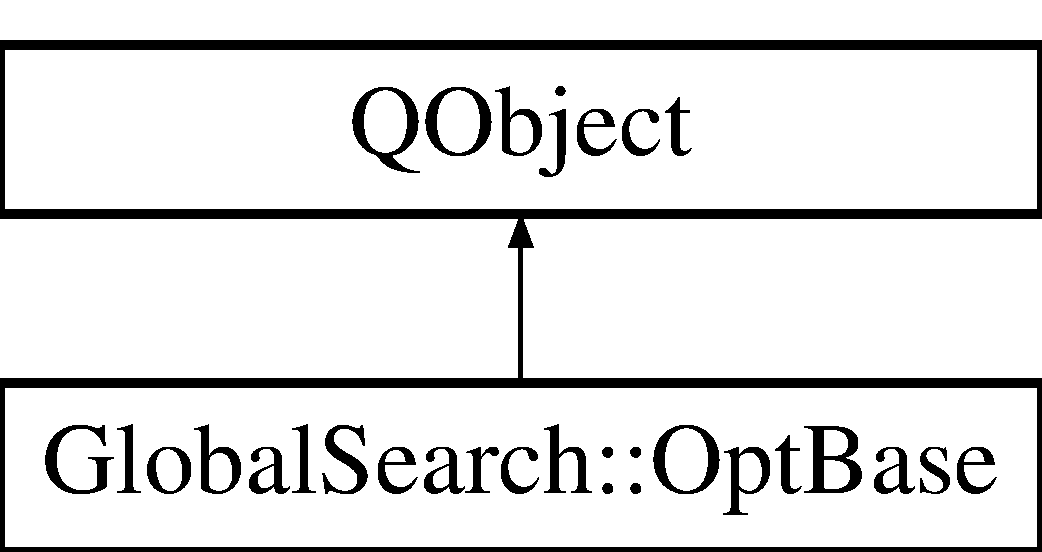
\includegraphics[height=2.000000cm]{classGlobalSearch_1_1OptBase}
\end{center}
\end{figure}
\subsection*{Public Types}
\begin{DoxyCompactItemize}
\item 
enum \hyperlink{classGlobalSearch_1_1OptBase_a970b328cd0a36335c34c6b24c6ac2775}{Fail\-Actions} \{ \hyperlink{classGlobalSearch_1_1OptBase_a970b328cd0a36335c34c6b24c6ac2775ab04d2d04ae7df7ba1da75a185c53dfca}{F\-A\-\_\-\-Do\-Nothing} = 0, 
\hyperlink{classGlobalSearch_1_1OptBase_a970b328cd0a36335c34c6b24c6ac2775a4457ab4b5903c890b0edf0817bf00e74}{F\-A\-\_\-\-Kill\-It}, 
\hyperlink{classGlobalSearch_1_1OptBase_a970b328cd0a36335c34c6b24c6ac2775a79cd7097c06d1b27824ae7c90201276a}{F\-A\-\_\-\-Randomize}, 
\hyperlink{classGlobalSearch_1_1OptBase_a970b328cd0a36335c34c6b24c6ac2775a548d59265329ca034e4e99257b85aa5e}{F\-A\-\_\-\-New\-Offspring}
 \}
\end{DoxyCompactItemize}
\subsection*{Public Slots}
\begin{DoxyCompactItemize}
\item 
virtual void \hyperlink{classGlobalSearch_1_1OptBase_aeb13548fad4b090a7e570011292fd389}{reset} ()
\item 
virtual void \hyperlink{classGlobalSearch_1_1OptBase_adc0d183586cb9433edc941ccea4cd1a4}{start\-Search} ()=0
\item 
virtual void \hyperlink{classGlobalSearch_1_1OptBase_a24b6e929232e6b82551c3917bf7dcc1c}{generate\-New\-Structure} ()
\item 
void \hyperlink{classGlobalSearch_1_1OptBase_a3e24cda71c456027edbcab36c9a5e08c}{debug} (const Q\-String \&s)
\item 
void \hyperlink{classGlobalSearch_1_1OptBase_a4f70a04b72a92665b7fb6f8e868b527e}{warning} (const Q\-String \&s)
\item 
void \hyperlink{classGlobalSearch_1_1OptBase_a0069abbd35393e6a5760b049e3497a21}{error} (const Q\-String \&s)
\item 
void \hyperlink{classGlobalSearch_1_1OptBase_ae71d020ca740d76941b66c682eea6986}{emit\-Session\-Started} ()
\item 
void \hyperlink{classGlobalSearch_1_1OptBase_ae1bd90daf659e169a56622d47f6a5be2}{emit\-Read\-Only\-Session\-Started} ()
\item 
void \hyperlink{classGlobalSearch_1_1OptBase_abbcfe0cbb229deb3781b718d175c14c2}{emit\-Starting\-Session} ()
\item 
void \hyperlink{classGlobalSearch_1_1OptBase_aa26f280c771034e15a1579057f4b5735}{set\-Is\-Starting\-True} ()
\item 
void \hyperlink{classGlobalSearch_1_1OptBase_a539171ea69cf4cfe55c08262e4af40f8}{set\-Is\-Starting\-False} ()
\item 
void \hyperlink{classGlobalSearch_1_1OptBase_a8f8fa9427077b974cbfc897089e34115}{set\-Read\-Only\-True} ()
\item 
void \hyperlink{classGlobalSearch_1_1OptBase_a284697394517be5888968af5c7716f6a}{set\-Read\-Only\-False} ()
\item 
void \hyperlink{classGlobalSearch_1_1OptBase_af00d6357f3ed311e9bcd2b03153fc3cc}{print\-Back\-Trace} ()
\item 
void \hyperlink{classGlobalSearch_1_1OptBase_add9178a3bfd695f1d42191a328956451}{set\-Queue\-Interface} (\hyperlink{classGlobalSearch_1_1QueueInterface}{Queue\-Interface} $\ast$q)
\item 
void \hyperlink{classGlobalSearch_1_1OptBase_addd46a192c8a68553a12b30d18246f1e}{set\-Optimizer} (\hyperlink{classGlobalSearch_1_1Optimizer}{Optimizer} $\ast$o)
\item 
void \hyperlink{classGlobalSearch_1_1OptBase_a3460f008a4a3cc3f8d00b3c0cd531069}{prompt\-For\-Boolean} (const Q\-String \&message, bool $\ast$ok=0)
\item 
void \hyperlink{classGlobalSearch_1_1OptBase_a934195fac431de2882383b0483505c95}{prompt\-For\-Password} (const Q\-String \&message, Q\-String $\ast$new\-Password, bool $\ast$ok=0)
\item 
void \hyperlink{classGlobalSearch_1_1OptBase_a3a509ee5a0aa4d8021dcb2d1bc34f1c1}{set\-Clipboard} (const Q\-String \&text) const 
\end{DoxyCompactItemize}
\subsection*{Signals}
\begin{DoxyCompactItemize}
\item 
void \hyperlink{classGlobalSearch_1_1OptBase_ac8b7b372d127a2ba9fada95645b4b4c7}{starting\-Session} ()
\item 
void \hyperlink{classGlobalSearch_1_1OptBase_a7d786f0cf4c5e95ea0b35e3b3c9eb87e}{session\-Started} ()
\item 
void \hyperlink{classGlobalSearch_1_1OptBase_a3d614aba63df12ea0e42e2b5cb0fe050}{read\-Only\-Session\-Started} ()
\item 
void \hyperlink{classGlobalSearch_1_1OptBase_ac1e2aa7f7dc57461fd12ff47b25e7c5c}{queue\-Interface\-Changed} (\hyperlink{classGlobalSearch_1_1QueueInterface}{Queue\-Interface} $\ast$)
\item 
void \hyperlink{classGlobalSearch_1_1OptBase_a8f07729ab8372e2a41de0d38d7947c6a}{optimizer\-Changed} (\hyperlink{classGlobalSearch_1_1Optimizer}{Optimizer} $\ast$)
\item 
void \hyperlink{classGlobalSearch_1_1OptBase_aa194f330e51154ce95a6cabb7fa4fccc}{debug\-Statement} (const Q\-String \&s)
\item 
void \hyperlink{classGlobalSearch_1_1OptBase_a70a45deb53ed3dbd6a1c2c458ea88afe}{warning\-Statement} (const Q\-String \&s)
\item 
void \hyperlink{classGlobalSearch_1_1OptBase_a6bcbb9a259f9173084e2f4a82ffa0b86}{error\-Statement} (const Q\-String \&s)
\item 
void \hyperlink{classGlobalSearch_1_1OptBase_a771c4b00f1fd857750ccb3d48116334d}{need\-Boolean} (const Q\-String \&message, bool $\ast$ok)
\item 
void \hyperlink{classGlobalSearch_1_1OptBase_aa140b7676a1fee73e1d416c164232fb3}{need\-Password} (const Q\-String \&message, Q\-String $\ast$new\-Password, bool $\ast$ok)
\item 
void \hyperlink{classGlobalSearch_1_1OptBase_a3d04c32b50632a6745cc013cf91d2551}{refresh\-All\-Structure\-Info} ()
\end{DoxyCompactItemize}
\subsection*{Public Member Functions}
\begin{DoxyCompactItemize}
\item 
\hyperlink{classGlobalSearch_1_1OptBase_a673110fb0bfe11da3f9f7811744c6578}{Opt\-Base} (\hyperlink{classGlobalSearch_1_1AbstractDialog}{Abstract\-Dialog} $\ast$parent)
\item 
virtual \hyperlink{classGlobalSearch_1_1OptBase_a8b5809d4bb0f97a2bad0ffc05c161f86}{$\sim$\-Opt\-Base} ()
\item 
Q\-String \hyperlink{classGlobalSearch_1_1OptBase_ae4223191dd58c47e186bbdf07f99ef1c}{get\-I\-D\-String} ()
\item 
virtual \hyperlink{classGlobalSearch_1_1Structure}{Structure} $\ast$ \hyperlink{classGlobalSearch_1_1OptBase_a8a370fdd83d4a157bb72fb0c865e31a4}{replace\-With\-Random} (\hyperlink{classGlobalSearch_1_1Structure}{Structure} $\ast$s, const Q\-String \&reason=\char`\"{}\char`\"{})
\item 
virtual \hyperlink{classGlobalSearch_1_1Structure}{Structure} $\ast$ \hyperlink{classGlobalSearch_1_1OptBase_a95ca1cb22a947989817c7cfc952cffbd}{replace\-With\-Offspring} (\hyperlink{classGlobalSearch_1_1Structure}{Structure} $\ast$s, const Q\-String \&reason=\char`\"{}\char`\"{})
\item 
virtual bool \hyperlink{classGlobalSearch_1_1OptBase_a406ca6399df3ef7fa545f3b34f90e0a4}{check\-Limits} ()=0
\item 
virtual bool \hyperlink{classGlobalSearch_1_1OptBase_abfacbe5ffa9d69db4e27bf6db2ad62f7}{save} (const Q\-String \&filename=\char`\"{}\char`\"{}, bool notify=false)
\item 
virtual bool \hyperlink{classGlobalSearch_1_1OptBase_a1d5e689eb327ccaf4c25f64e83e5678b}{load} (const Q\-String \&filename, const bool force\-Read\-Only=false)
\item 
virtual Q\-String \hyperlink{classGlobalSearch_1_1OptBase_a238dbb50b8d7aac7a6660613397565f0}{interpret\-Template} (const Q\-String \&template\-String, \hyperlink{classGlobalSearch_1_1Structure}{Structure} $\ast$structure)
\item 
virtual Q\-String \hyperlink{classGlobalSearch_1_1OptBase_a79650b4bd0dde4580a98a89e7032be96}{get\-Template\-Keyword\-Help} ()
\item 
\hyperlink{classGlobalSearch_1_1AbstractDialog}{Abstract\-Dialog} $\ast$ \hyperlink{classGlobalSearch_1_1OptBase_a3ccbd5949beb6e1efac734da29b726b7}{dialog} ()
\item 
\hyperlink{classGlobalSearch_1_1Tracker}{Tracker} $\ast$ \hyperlink{classGlobalSearch_1_1OptBase_a304d0d10064bd3913c8089aca76067d6}{tracker} ()
\item 
\hyperlink{classGlobalSearch_1_1QueueManager}{Queue\-Manager} $\ast$ \hyperlink{classGlobalSearch_1_1OptBase_aa10982ae8ea63745203a025b2be8054d}{queue} ()
\item 
\hyperlink{classGlobalSearch_1_1QueueInterface}{Queue\-Interface} $\ast$ \hyperlink{classGlobalSearch_1_1OptBase_a73faf60edcd3db57538349f5a636576e}{queue\-Interface} ()
\item 
\hyperlink{classGlobalSearch_1_1Optimizer}{Optimizer} $\ast$ \hyperlink{classGlobalSearch_1_1OptBase_a4dce62d15f24d665c807047aa5c618fc}{optimizer} ()
\item 
S\-S\-H\-Manager $\ast$ \hyperlink{classGlobalSearch_1_1OptBase_a40064a3c1e6d0acae26b1908a8bdf5db}{ssh} ()
\end{DoxyCompactItemize}
\subsection*{Static Public Member Functions}
\begin{DoxyCompactItemize}
\item 
static Q\-List$<$ double $>$ \hyperlink{classGlobalSearch_1_1OptBase_a863b23c21cf06829e39420fcc94f0348}{get\-Probability\-List} (const Q\-List$<$ \hyperlink{classGlobalSearch_1_1Structure}{Structure} $\ast$ $>$ \&structures)
\end{DoxyCompactItemize}
\subsection*{Public Attributes}
\begin{DoxyCompactItemize}
\item 
\hypertarget{classGlobalSearch_1_1OptBase_a3b5202a4793e24dd7d42d1df9e94ee27}{bool \hyperlink{classGlobalSearch_1_1OptBase_a3b5202a4793e24dd7d42d1df9e94ee27}{limit\-Running\-Jobs}}\label{classGlobalSearch_1_1OptBase_a3b5202a4793e24dd7d42d1df9e94ee27}

\begin{DoxyCompactList}\small\item\em Whether to impose the running job limit. \end{DoxyCompactList}\item 
\hypertarget{classGlobalSearch_1_1OptBase_a02fd48b57bdd72ec4a4c20209967bd07}{uint \hyperlink{classGlobalSearch_1_1OptBase_a02fd48b57bdd72ec4a4c20209967bd07}{running\-Job\-Limit}}\label{classGlobalSearch_1_1OptBase_a02fd48b57bdd72ec4a4c20209967bd07}

\begin{DoxyCompactList}\small\item\em Number of concurrent jobs allowed. \end{DoxyCompactList}\item 
\hypertarget{classGlobalSearch_1_1OptBase_a973fbcff3e2abbc66c19236092439ce1}{uint \hyperlink{classGlobalSearch_1_1OptBase_a973fbcff3e2abbc66c19236092439ce1}{cont\-Structs}}\label{classGlobalSearch_1_1OptBase_a973fbcff3e2abbc66c19236092439ce1}

\begin{DoxyCompactList}\small\item\em Number of continuous structures generated. \end{DoxyCompactList}\item 
\hypertarget{classGlobalSearch_1_1OptBase_a6fe1eb9eef50d0c0851c7113cc8f24f0}{int \hyperlink{classGlobalSearch_1_1OptBase_a6fe1eb9eef50d0c0851c7113cc8f24f0}{cutoff}}\label{classGlobalSearch_1_1OptBase_a6fe1eb9eef50d0c0851c7113cc8f24f0}

\begin{DoxyCompactList}\small\item\em How many structures to produce before halting search. -\/1 for no limit. \end{DoxyCompactList}\item 
\hypertarget{classGlobalSearch_1_1OptBase_a4aee28dd2991e1ada81243d05a1f23c9}{bool \hyperlink{classGlobalSearch_1_1OptBase_a4aee28dd2991e1ada81243d05a1f23c9}{testing\-Mode}}\label{classGlobalSearch_1_1OptBase_a4aee28dd2991e1ada81243d05a1f23c9}

\begin{DoxyCompactList}\small\item\em Whether to run benchmarking tests. \end{DoxyCompactList}\item 
\hypertarget{classGlobalSearch_1_1OptBase_a8d8902d09ca98a8f078182394bd1d7a1}{uint \hyperlink{classGlobalSearch_1_1OptBase_a8d8902d09ca98a8f078182394bd1d7a1}{test\-\_\-n\-Runs\-Start}}\label{classGlobalSearch_1_1OptBase_a8d8902d09ca98a8f078182394bd1d7a1}

\begin{DoxyCompactList}\small\item\em Starting run number for benchmark. \end{DoxyCompactList}\item 
\hypertarget{classGlobalSearch_1_1OptBase_a3433cbd854cbbb5d350e2ba7bb665c44}{uint \hyperlink{classGlobalSearch_1_1OptBase_a3433cbd854cbbb5d350e2ba7bb665c44}{test\-\_\-n\-Runs\-End}}\label{classGlobalSearch_1_1OptBase_a3433cbd854cbbb5d350e2ba7bb665c44}

\begin{DoxyCompactList}\small\item\em Ending run number for benchmark. \end{DoxyCompactList}\item 
\hypertarget{classGlobalSearch_1_1OptBase_a973157ab02d197102e5f67d80aacd706}{uint \hyperlink{classGlobalSearch_1_1OptBase_a973157ab02d197102e5f67d80aacd706}{test\-\_\-n\-Structs}}\label{classGlobalSearch_1_1OptBase_a973157ab02d197102e5f67d80aacd706}

\begin{DoxyCompactList}\small\item\em Number of Structures per run when benchmarking. \end{DoxyCompactList}\item 
uint \hyperlink{classGlobalSearch_1_1OptBase_aec8bb712a35c23ab79608a5d70f52b90}{fail\-Limit}
\item 
\hyperlink{classGlobalSearch_1_1OptBase_a970b328cd0a36335c34c6b24c6ac2775}{Fail\-Actions} \hyperlink{classGlobalSearch_1_1OptBase_adda17a1eab956c00c6b14ab3ae451b91}{fail\-Action}
\item 
\hypertarget{classGlobalSearch_1_1OptBase_a707d2bf2511d4fec3f244afb2f094c6e}{Q\-String \hyperlink{classGlobalSearch_1_1OptBase_a707d2bf2511d4fec3f244afb2f094c6e}{file\-Path}}\label{classGlobalSearch_1_1OptBase_a707d2bf2511d4fec3f244afb2f094c6e}

\begin{DoxyCompactList}\small\item\em Local directory to work in. \end{DoxyCompactList}\item 
\hypertarget{classGlobalSearch_1_1OptBase_ae7a73ff186f939f8fab1647a2dea6872}{Q\-String \hyperlink{classGlobalSearch_1_1OptBase_ae7a73ff186f939f8fab1647a2dea6872}{description}}\label{classGlobalSearch_1_1OptBase_ae7a73ff186f939f8fab1647a2dea6872}

\begin{DoxyCompactList}\small\item\em Terse description of current search. \end{DoxyCompactList}\item 
\hypertarget{classGlobalSearch_1_1OptBase_a450b588c2994270e8e053365f094fb52}{Q\-String \hyperlink{classGlobalSearch_1_1OptBase_a450b588c2994270e8e053365f094fb52}{host}}\label{classGlobalSearch_1_1OptBase_a450b588c2994270e8e053365f094fb52}

\begin{DoxyCompactList}\small\item\em Host name or I\-P address of remote P\-B\-S server. \end{DoxyCompactList}\item 
\hypertarget{classGlobalSearch_1_1OptBase_aa07a4fe47df0f8d4fface200fdde4dee}{int \hyperlink{classGlobalSearch_1_1OptBase_aa07a4fe47df0f8d4fface200fdde4dee}{port}}\label{classGlobalSearch_1_1OptBase_aa07a4fe47df0f8d4fface200fdde4dee}

\begin{DoxyCompactList}\small\item\em Port on remote P\-B\-S server used for S\-S\-H communication. \end{DoxyCompactList}\item 
\hypertarget{classGlobalSearch_1_1OptBase_a75c9102491957d00fd6bd4da9329c2ed}{Q\-String \hyperlink{classGlobalSearch_1_1OptBase_a75c9102491957d00fd6bd4da9329c2ed}{username}}\label{classGlobalSearch_1_1OptBase_a75c9102491957d00fd6bd4da9329c2ed}

\begin{DoxyCompactList}\small\item\em Username for ssh login on remote P\-B\-S server. \end{DoxyCompactList}\item 
Q\-String \hyperlink{classGlobalSearch_1_1OptBase_a777ad7fbedbb76f522e02ca73883ab7d}{rempath}
\item 
Q\-Mutex $\ast$ \hyperlink{classGlobalSearch_1_1OptBase_a86c1868458b6f8430dc366c009c9deb5}{s\-O\-B\-Mutex}
\item 
Q\-Mutex $\ast$ \hyperlink{classGlobalSearch_1_1OptBase_af0df28a179c8a89022f4887c18761956}{state\-File\-Mutex}
\item 
\hypertarget{classGlobalSearch_1_1OptBase_aa74d5687ec2969388db9c4a87adbfce5}{Q\-Mutex $\ast$ \hyperlink{classGlobalSearch_1_1OptBase_aa74d5687ec2969388db9c4a87adbfce5}{back\-Trace\-Mutex}}\label{classGlobalSearch_1_1OptBase_aa74d5687ec2969388db9c4a87adbfce5}

\begin{DoxyCompactList}\small\item\em This is locked when generating a backtrace. \end{DoxyCompactList}\item 
\hypertarget{classGlobalSearch_1_1OptBase_a2e5ba27bde6be3257cc44b7a7bb87598}{bool \hyperlink{classGlobalSearch_1_1OptBase_a2e5ba27bde6be3257cc44b7a7bb87598}{save\-Pending}}\label{classGlobalSearch_1_1OptBase_a2e5ba27bde6be3257cc44b7a7bb87598}

\begin{DoxyCompactList}\small\item\em True if there is a save requested or in progress. \end{DoxyCompactList}\item 
\hypertarget{classGlobalSearch_1_1OptBase_a63828837cb869c94cb7309cbb7331f7c}{bool \hyperlink{classGlobalSearch_1_1OptBase_a63828837cb869c94cb7309cbb7331f7c}{is\-Starting}}\label{classGlobalSearch_1_1OptBase_a63828837cb869c94cb7309cbb7331f7c}

\begin{DoxyCompactList}\small\item\em True if a session is starting or being loaded. \end{DoxyCompactList}\item 
\hypertarget{classGlobalSearch_1_1OptBase_ac85d94d2e3b44f66461e470e04db3f0e}{bool \hyperlink{classGlobalSearch_1_1OptBase_ac85d94d2e3b44f66461e470e04db3f0e}{read\-Only}}\label{classGlobalSearch_1_1OptBase_ac85d94d2e3b44f66461e470e04db3f0e}

\begin{DoxyCompactList}\small\item\em Whether read\-Only mode is enabled (e.\-g. no connection to server) \end{DoxyCompactList}\end{DoxyCompactItemize}
\subsection*{Protected Member Functions}
\begin{DoxyCompactItemize}
\item 
\hypertarget{classGlobalSearch_1_1OptBase_abff4ef4b7e717351103658ff33dfa561}{void \hyperlink{classGlobalSearch_1_1OptBase_abff4ef4b7e717351103658ff33dfa561}{interpret\-Keyword\-\_\-base} (Q\-String \&keyword, \hyperlink{classGlobalSearch_1_1Structure}{Structure} $\ast$structure)}\label{classGlobalSearch_1_1OptBase_abff4ef4b7e717351103658ff33dfa561}

\begin{DoxyCompactList}\small\item\em Hidden call to interpret\-Keyword. \end{DoxyCompactList}\item 
\hypertarget{classGlobalSearch_1_1OptBase_a41a41f9733da4a68244bc56195ea835b}{Q\-String \hyperlink{classGlobalSearch_1_1OptBase_a41a41f9733da4a68244bc56195ea835b}{get\-Template\-Keyword\-Help\-\_\-base} ()}\label{classGlobalSearch_1_1OptBase_a41a41f9733da4a68244bc56195ea835b}

\begin{DoxyCompactList}\small\item\em Hidden call to get\-Template\-Keyword\-Help. \end{DoxyCompactList}\end{DoxyCompactItemize}
\subsection*{Protected Attributes}
\begin{DoxyCompactItemize}
\item 
Q\-String \hyperlink{classGlobalSearch_1_1OptBase_af9223062bbb616246d5bf60ad29e1c7d}{m\-\_\-id\-String}
\item 
S\-S\-H\-Manager $\ast$ \hyperlink{classGlobalSearch_1_1OptBase_a723a6dd0bb93aff451007ccb079e2f65}{m\-\_\-ssh}
\item 
\hyperlink{classGlobalSearch_1_1AbstractDialog}{Abstract\-Dialog} $\ast$ \hyperlink{classGlobalSearch_1_1OptBase_a4673e81b57e648320474bf3024906161}{m\-\_\-dialog}
\item 
\hyperlink{classGlobalSearch_1_1Tracker}{Tracker} $\ast$ \hyperlink{classGlobalSearch_1_1OptBase_a60a2c6053a8ae3716854c68d0837b921}{m\-\_\-tracker}
\item 
\hypertarget{classGlobalSearch_1_1OptBase_a80b28eb1b9d8d7a055ddabb55c753f20}{Q\-Thread $\ast$ \hyperlink{classGlobalSearch_1_1OptBase_a80b28eb1b9d8d7a055ddabb55c753f20}{m\-\_\-queue\-Thread}}\label{classGlobalSearch_1_1OptBase_a80b28eb1b9d8d7a055ddabb55c753f20}

\begin{DoxyCompactList}\small\item\em Thread to run the \hyperlink{classGlobalSearch_1_1QueueManager}{Queue\-Manager}. \end{DoxyCompactList}\item 
\hyperlink{classGlobalSearch_1_1QueueManager}{Queue\-Manager} $\ast$ \hyperlink{classGlobalSearch_1_1OptBase_a187a29ceafe0c4a45ecb7a925267f93a}{m\-\_\-queue}
\item 
\hyperlink{classGlobalSearch_1_1QueueInterface}{Queue\-Interface} $\ast$ \hyperlink{classGlobalSearch_1_1OptBase_a8f5f83dae1456bbff32ea9b3b6731ba0}{m\-\_\-queue\-Interface}
\item 
\hyperlink{classGlobalSearch_1_1Optimizer}{Optimizer} $\ast$ \hyperlink{classGlobalSearch_1_1OptBase_a9bc76450b0d52ab9fc9a4caaf97143b7}{m\-\_\-optimizer}
\item 
\hypertarget{classGlobalSearch_1_1OptBase_a7e2fe2db52705fd57edf9178e03345bd}{unsigned int \hyperlink{classGlobalSearch_1_1OptBase_a7e2fe2db52705fd57edf9178e03345bd}{m\-\_\-schema\-Version}}\label{classGlobalSearch_1_1OptBase_a7e2fe2db52705fd57edf9178e03345bd}

\begin{DoxyCompactList}\small\item\em Current version of save/resume schema. \end{DoxyCompactList}\end{DoxyCompactItemize}


\subsection{Detailed Description}
The \hyperlink{classGlobalSearch_1_1OptBase}{Opt\-Base} class stores variables and helper functions for global searches. 

\begin{DoxyAuthor}{Author}
David C. Lonie
\end{DoxyAuthor}
\hyperlink{classGlobalSearch_1_1OptBase}{Opt\-Base} is the main class in libglobalsearch. It contains the variables that define a search, as well as handling structure generation. This class ties all others together. 

Definition at line 53 of file optbase.\-h.



\subsection{Member Enumeration Documentation}
\hypertarget{classGlobalSearch_1_1OptBase_a970b328cd0a36335c34c6b24c6ac2775}{\index{Global\-Search\-::\-Opt\-Base@{Global\-Search\-::\-Opt\-Base}!Fail\-Actions@{Fail\-Actions}}
\index{Fail\-Actions@{Fail\-Actions}!GlobalSearch::OptBase@{Global\-Search\-::\-Opt\-Base}}
\subsubsection[{Fail\-Actions}]{\setlength{\rightskip}{0pt plus 5cm}enum {\bf Global\-Search\-::\-Opt\-Base\-::\-Fail\-Actions}}}\label{classGlobalSearch_1_1OptBase_a970b328cd0a36335c34c6b24c6ac2775}
Actions to take when a structure has failed optimization too many times.

\begin{DoxySeeAlso}{See Also}
\hyperlink{classGlobalSearch_1_1OptBase_adda17a1eab956c00c6b14ab3ae451b91}{Opt\-Base\-::fail\-Action} 

\hyperlink{classGlobalSearch_1_1OptBase_aec8bb712a35c23ab79608a5d70f52b90}{Opt\-Base\-::fail\-Limit} 
\end{DoxySeeAlso}
\begin{Desc}
\item[Enumerator]\par
\begin{description}
\index{F\-A\-\_\-\-Do\-Nothing@{F\-A\-\_\-\-Do\-Nothing}!Global\-Search\-::\-Opt\-Base@{Global\-Search\-::\-Opt\-Base}}\index{Global\-Search\-::\-Opt\-Base@{Global\-Search\-::\-Opt\-Base}!F\-A\-\_\-\-Do\-Nothing@{F\-A\-\_\-\-Do\-Nothing}}\item[{\em 
\hypertarget{classGlobalSearch_1_1OptBase_a970b328cd0a36335c34c6b24c6ac2775ab04d2d04ae7df7ba1da75a185c53dfca}{F\-A\-\_\-\-Do\-Nothing}\label{classGlobalSearch_1_1OptBase_a970b328cd0a36335c34c6b24c6ac2775ab04d2d04ae7df7ba1da75a185c53dfca}
}]Do nothing; keep submitting for optimization. \index{F\-A\-\_\-\-Kill\-It@{F\-A\-\_\-\-Kill\-It}!Global\-Search\-::\-Opt\-Base@{Global\-Search\-::\-Opt\-Base}}\index{Global\-Search\-::\-Opt\-Base@{Global\-Search\-::\-Opt\-Base}!F\-A\-\_\-\-Kill\-It@{F\-A\-\_\-\-Kill\-It}}\item[{\em 
\hypertarget{classGlobalSearch_1_1OptBase_a970b328cd0a36335c34c6b24c6ac2775a4457ab4b5903c890b0edf0817bf00e74}{F\-A\-\_\-\-Kill\-It}\label{classGlobalSearch_1_1OptBase_a970b328cd0a36335c34c6b24c6ac2775a4457ab4b5903c890b0edf0817bf00e74}
}]Kill the structure. \index{F\-A\-\_\-\-Randomize@{F\-A\-\_\-\-Randomize}!Global\-Search\-::\-Opt\-Base@{Global\-Search\-::\-Opt\-Base}}\index{Global\-Search\-::\-Opt\-Base@{Global\-Search\-::\-Opt\-Base}!F\-A\-\_\-\-Randomize@{F\-A\-\_\-\-Randomize}}\item[{\em 
\hypertarget{classGlobalSearch_1_1OptBase_a970b328cd0a36335c34c6b24c6ac2775a79cd7097c06d1b27824ae7c90201276a}{F\-A\-\_\-\-Randomize}\label{classGlobalSearch_1_1OptBase_a970b328cd0a36335c34c6b24c6ac2775a79cd7097c06d1b27824ae7c90201276a}
}]Replace the failing structure with a new random one. \index{F\-A\-\_\-\-New\-Offspring@{F\-A\-\_\-\-New\-Offspring}!Global\-Search\-::\-Opt\-Base@{Global\-Search\-::\-Opt\-Base}}\index{Global\-Search\-::\-Opt\-Base@{Global\-Search\-::\-Opt\-Base}!F\-A\-\_\-\-New\-Offspring@{F\-A\-\_\-\-New\-Offspring}}\item[{\em 
\hypertarget{classGlobalSearch_1_1OptBase_a970b328cd0a36335c34c6b24c6ac2775a548d59265329ca034e4e99257b85aa5e}{F\-A\-\_\-\-New\-Offspring}\label{classGlobalSearch_1_1OptBase_a970b328cd0a36335c34c6b24c6ac2775a548d59265329ca034e4e99257b85aa5e}
}]Replace with a new offspring structure. \end{description}
\end{Desc}


Definition at line 77 of file optbase.\-h.



\subsection{Constructor \& Destructor Documentation}
\hypertarget{classGlobalSearch_1_1OptBase_a673110fb0bfe11da3f9f7811744c6578}{\index{Global\-Search\-::\-Opt\-Base@{Global\-Search\-::\-Opt\-Base}!Opt\-Base@{Opt\-Base}}
\index{Opt\-Base@{Opt\-Base}!GlobalSearch::OptBase@{Global\-Search\-::\-Opt\-Base}}
\subsubsection[{Opt\-Base}]{\setlength{\rightskip}{0pt plus 5cm}Global\-Search\-::\-Opt\-Base\-::\-Opt\-Base (
\begin{DoxyParamCaption}
\item[{{\bf Abstract\-Dialog} $\ast$}]{parent}
\end{DoxyParamCaption}
)\hspace{0.3cm}{\ttfamily [explicit]}}}\label{classGlobalSearch_1_1OptBase_a673110fb0bfe11da3f9f7811744c6578}
Constructor


\begin{DoxyParams}{Parameters}
{\em parent} & Dialog window of G\-U\-I. \\
\hline
\end{DoxyParams}


Definition at line 48 of file optbase.\-cpp.



References m\-\_\-queue\-Thread, need\-Boolean(), need\-Password(), prompt\-For\-Boolean(), prompt\-For\-Password(), read\-Only\-Session\-Started(), session\-Started(), set\-Is\-Starting\-False(), set\-Is\-Starting\-True(), and starting\-Session().

\hypertarget{classGlobalSearch_1_1OptBase_a8b5809d4bb0f97a2bad0ffc05c161f86}{\index{Global\-Search\-::\-Opt\-Base@{Global\-Search\-::\-Opt\-Base}!$\sim$\-Opt\-Base@{$\sim$\-Opt\-Base}}
\index{$\sim$\-Opt\-Base@{$\sim$\-Opt\-Base}!GlobalSearch::OptBase@{Global\-Search\-::\-Opt\-Base}}
\subsubsection[{$\sim$\-Opt\-Base}]{\setlength{\rightskip}{0pt plus 5cm}Global\-Search\-::\-Opt\-Base\-::$\sim$\-Opt\-Base (
\begin{DoxyParamCaption}
{}
\end{DoxyParamCaption}
)\hspace{0.3cm}{\ttfamily [virtual]}}}\label{classGlobalSearch_1_1OptBase_a8b5809d4bb0f97a2bad0ffc05c161f86}
Destructor 

Definition at line 101 of file optbase.\-cpp.



References m\-\_\-optimizer, m\-\_\-queue, m\-\_\-queue\-Interface, m\-\_\-queue\-Thread, and m\-\_\-tracker.



\subsection{Member Function Documentation}
\hypertarget{classGlobalSearch_1_1OptBase_a406ca6399df3ef7fa545f3b34f90e0a4}{\index{Global\-Search\-::\-Opt\-Base@{Global\-Search\-::\-Opt\-Base}!check\-Limits@{check\-Limits}}
\index{check\-Limits@{check\-Limits}!GlobalSearch::OptBase@{Global\-Search\-::\-Opt\-Base}}
\subsubsection[{check\-Limits}]{\setlength{\rightskip}{0pt plus 5cm}virtual bool Global\-Search\-::\-Opt\-Base\-::check\-Limits (
\begin{DoxyParamCaption}
{}
\end{DoxyParamCaption}
)\hspace{0.3cm}{\ttfamily [pure virtual]}}}\label{classGlobalSearch_1_1OptBase_a406ca6399df3ef7fa545f3b34f90e0a4}
Before starting an optimization, this function will check the parameters of the search to ensure that they are within a reasonable range.

\begin{DoxyReturn}{Returns}
True if the search parameters are valid, false otherwise. 
\end{DoxyReturn}
\hypertarget{classGlobalSearch_1_1OptBase_a3e24cda71c456027edbcab36c9a5e08c}{\index{Global\-Search\-::\-Opt\-Base@{Global\-Search\-::\-Opt\-Base}!debug@{debug}}
\index{debug@{debug}!GlobalSearch::OptBase@{Global\-Search\-::\-Opt\-Base}}
\subsubsection[{debug}]{\setlength{\rightskip}{0pt plus 5cm}void Global\-Search\-::\-Opt\-Base\-::debug (
\begin{DoxyParamCaption}
\item[{const Q\-String \&}]{s}
\end{DoxyParamCaption}
)\hspace{0.3cm}{\ttfamily [slot]}}}\label{classGlobalSearch_1_1OptBase_a3e24cda71c456027edbcab36c9a5e08c}
Prints a debug message to the terminal and emits debug\-Statement 
\begin{DoxyParams}{Parameters}
{\em s} & The debug statement. \\
\hline
\end{DoxyParams}
\begin{DoxySeeAlso}{See Also}
\hyperlink{classGlobalSearch_1_1OptBase_a3e24cda71c456027edbcab36c9a5e08c}{debug} 

\hyperlink{classGlobalSearch_1_1OptBase_aa194f330e51154ce95a6cabb7fa4fccc}{debug\-Statement} 

\hyperlink{classGlobalSearch_1_1OptBase_a4f70a04b72a92665b7fb6f8e868b527e}{warning} 

\hyperlink{classGlobalSearch_1_1OptBase_a70a45deb53ed3dbd6a1c2c458ea88afe}{warning\-Statement} 

\hyperlink{classGlobalSearch_1_1OptBase_a0069abbd35393e6a5760b049e3497a21}{error} 

\hyperlink{classGlobalSearch_1_1OptBase_a6bcbb9a259f9173084e2f4a82ffa0b86}{error\-Statement} 
\end{DoxySeeAlso}


Definition at line 608 of file optbase.\-cpp.



References debug\-Statement().

\hypertarget{classGlobalSearch_1_1OptBase_aa194f330e51154ce95a6cabb7fa4fccc}{\index{Global\-Search\-::\-Opt\-Base@{Global\-Search\-::\-Opt\-Base}!debug\-Statement@{debug\-Statement}}
\index{debug\-Statement@{debug\-Statement}!GlobalSearch::OptBase@{Global\-Search\-::\-Opt\-Base}}
\subsubsection[{debug\-Statement}]{\setlength{\rightskip}{0pt plus 5cm}void Global\-Search\-::\-Opt\-Base\-::debug\-Statement (
\begin{DoxyParamCaption}
\item[{const Q\-String \&}]{s}
\end{DoxyParamCaption}
)\hspace{0.3cm}{\ttfamily [signal]}}}\label{classGlobalSearch_1_1OptBase_aa194f330e51154ce95a6cabb7fa4fccc}
Emitted when \hyperlink{classGlobalSearch_1_1OptBase_a3e24cda71c456027edbcab36c9a5e08c}{debug(const Q\-String\&)} is called. 
\begin{DoxyParams}{Parameters}
{\em s} & The debugging statement. \\
\hline
\end{DoxyParams}
\begin{DoxySeeAlso}{See Also}
\hyperlink{classGlobalSearch_1_1OptBase_a3e24cda71c456027edbcab36c9a5e08c}{debug} 

\hyperlink{classGlobalSearch_1_1OptBase_aa194f330e51154ce95a6cabb7fa4fccc}{debug\-Statement} 

\hyperlink{classGlobalSearch_1_1OptBase_a4f70a04b72a92665b7fb6f8e868b527e}{warning} 

\hyperlink{classGlobalSearch_1_1OptBase_a70a45deb53ed3dbd6a1c2c458ea88afe}{warning\-Statement} 

\hyperlink{classGlobalSearch_1_1OptBase_a0069abbd35393e6a5760b049e3497a21}{error} 

\hyperlink{classGlobalSearch_1_1OptBase_a6bcbb9a259f9173084e2f4a82ffa0b86}{error\-Statement} 
\end{DoxySeeAlso}


Referenced by debug().

\hypertarget{classGlobalSearch_1_1OptBase_a3ccbd5949beb6e1efac734da29b726b7}{\index{Global\-Search\-::\-Opt\-Base@{Global\-Search\-::\-Opt\-Base}!dialog@{dialog}}
\index{dialog@{dialog}!GlobalSearch::OptBase@{Global\-Search\-::\-Opt\-Base}}
\subsubsection[{dialog}]{\setlength{\rightskip}{0pt plus 5cm}{\bf Abstract\-Dialog}$\ast$ Global\-Search\-::\-Opt\-Base\-::dialog (
\begin{DoxyParamCaption}
{}
\end{DoxyParamCaption}
)\hspace{0.3cm}{\ttfamily [inline]}}}\label{classGlobalSearch_1_1OptBase_a3ccbd5949beb6e1efac734da29b726b7}
\begin{DoxyReturn}{Returns}
A pointer to the main dialog.. 
\end{DoxyReturn}


Definition at line 218 of file optbase.\-h.



References m\-\_\-dialog.



Referenced by Global\-Search\-::\-Local\-Queue\-Interface\-::dialog(), Global\-Search\-::\-Optimizer\-::dialog(), prompt\-For\-Boolean(), and prompt\-For\-Password().

\hypertarget{classGlobalSearch_1_1OptBase_ae1bd90daf659e169a56622d47f6a5be2}{\index{Global\-Search\-::\-Opt\-Base@{Global\-Search\-::\-Opt\-Base}!emit\-Read\-Only\-Session\-Started@{emit\-Read\-Only\-Session\-Started}}
\index{emit\-Read\-Only\-Session\-Started@{emit\-Read\-Only\-Session\-Started}!GlobalSearch::OptBase@{Global\-Search\-::\-Opt\-Base}}
\subsubsection[{emit\-Read\-Only\-Session\-Started}]{\setlength{\rightskip}{0pt plus 5cm}void Global\-Search\-::\-Opt\-Base\-::emit\-Read\-Only\-Session\-Started (
\begin{DoxyParamCaption}
{}
\end{DoxyParamCaption}
)\hspace{0.3cm}{\ttfamily [inline]}, {\ttfamily [slot]}}}\label{classGlobalSearch_1_1OptBase_ae1bd90daf659e169a56622d47f6a5be2}
Emits the read\-Only\-Session\-Started signal. \begin{DoxySeeAlso}{See Also}
\hyperlink{classGlobalSearch_1_1OptBase_a7d786f0cf4c5e95ea0b35e3b3c9eb87e}{session\-Started} 

\hyperlink{classGlobalSearch_1_1OptBase_ae71d020ca740d76941b66c682eea6986}{emit\-Session\-Started} 

\hyperlink{classGlobalSearch_1_1OptBase_a3d614aba63df12ea0e42e2b5cb0fe050}{read\-Only\-Session\-Started} 

\hyperlink{classGlobalSearch_1_1OptBase_ac8b7b372d127a2ba9fada95645b4b4c7}{starting\-Session} 

\hyperlink{classGlobalSearch_1_1OptBase_abbcfe0cbb229deb3781b718d175c14c2}{emit\-Starting\-Session} 
\end{DoxySeeAlso}


Definition at line 523 of file optbase.\-h.



References read\-Only\-Session\-Started().



Referenced by Global\-Search\-::\-Abstract\-Dialog\-::resume\-Session\-\_\-().

\hypertarget{classGlobalSearch_1_1OptBase_ae71d020ca740d76941b66c682eea6986}{\index{Global\-Search\-::\-Opt\-Base@{Global\-Search\-::\-Opt\-Base}!emit\-Session\-Started@{emit\-Session\-Started}}
\index{emit\-Session\-Started@{emit\-Session\-Started}!GlobalSearch::OptBase@{Global\-Search\-::\-Opt\-Base}}
\subsubsection[{emit\-Session\-Started}]{\setlength{\rightskip}{0pt plus 5cm}void Global\-Search\-::\-Opt\-Base\-::emit\-Session\-Started (
\begin{DoxyParamCaption}
{}
\end{DoxyParamCaption}
)\hspace{0.3cm}{\ttfamily [inline]}, {\ttfamily [slot]}}}\label{classGlobalSearch_1_1OptBase_ae71d020ca740d76941b66c682eea6986}
Emits the session\-Started signal. \begin{DoxySeeAlso}{See Also}
\hyperlink{classGlobalSearch_1_1OptBase_a7d786f0cf4c5e95ea0b35e3b3c9eb87e}{session\-Started} 

\hyperlink{classGlobalSearch_1_1OptBase_a3d614aba63df12ea0e42e2b5cb0fe050}{read\-Only\-Session\-Started} 

\hyperlink{classGlobalSearch_1_1OptBase_ae1bd90daf659e169a56622d47f6a5be2}{emit\-Read\-Only\-Session\-Started} 

\hyperlink{classGlobalSearch_1_1OptBase_ac8b7b372d127a2ba9fada95645b4b4c7}{starting\-Session} 

\hyperlink{classGlobalSearch_1_1OptBase_abbcfe0cbb229deb3781b718d175c14c2}{emit\-Starting\-Session} 
\end{DoxySeeAlso}


Definition at line 513 of file optbase.\-h.



References session\-Started().



Referenced by Global\-Search\-::\-Abstract\-Dialog\-::resume\-Session\-\_\-().

\hypertarget{classGlobalSearch_1_1OptBase_abbcfe0cbb229deb3781b718d175c14c2}{\index{Global\-Search\-::\-Opt\-Base@{Global\-Search\-::\-Opt\-Base}!emit\-Starting\-Session@{emit\-Starting\-Session}}
\index{emit\-Starting\-Session@{emit\-Starting\-Session}!GlobalSearch::OptBase@{Global\-Search\-::\-Opt\-Base}}
\subsubsection[{emit\-Starting\-Session}]{\setlength{\rightskip}{0pt plus 5cm}void Global\-Search\-::\-Opt\-Base\-::emit\-Starting\-Session (
\begin{DoxyParamCaption}
{}
\end{DoxyParamCaption}
)\hspace{0.3cm}{\ttfamily [inline]}, {\ttfamily [slot]}}}\label{classGlobalSearch_1_1OptBase_abbcfe0cbb229deb3781b718d175c14c2}
Emits the starting\-Session signal. \begin{DoxySeeAlso}{See Also}
\hyperlink{classGlobalSearch_1_1OptBase_a7d786f0cf4c5e95ea0b35e3b3c9eb87e}{session\-Started} 

\hyperlink{classGlobalSearch_1_1OptBase_ae71d020ca740d76941b66c682eea6986}{emit\-Session\-Started} 

\hyperlink{classGlobalSearch_1_1OptBase_ac8b7b372d127a2ba9fada95645b4b4c7}{starting\-Session} 

\hyperlink{classGlobalSearch_1_1OptBase_abbcfe0cbb229deb3781b718d175c14c2}{emit\-Starting\-Session} 
\end{DoxySeeAlso}


Definition at line 532 of file optbase.\-h.



References starting\-Session().



Referenced by Global\-Search\-::\-Abstract\-Dialog\-::resume\-Session\-\_\-().

\hypertarget{classGlobalSearch_1_1OptBase_a0069abbd35393e6a5760b049e3497a21}{\index{Global\-Search\-::\-Opt\-Base@{Global\-Search\-::\-Opt\-Base}!error@{error}}
\index{error@{error}!GlobalSearch::OptBase@{Global\-Search\-::\-Opt\-Base}}
\subsubsection[{error}]{\setlength{\rightskip}{0pt plus 5cm}void Global\-Search\-::\-Opt\-Base\-::error (
\begin{DoxyParamCaption}
\item[{const Q\-String \&}]{s}
\end{DoxyParamCaption}
)\hspace{0.3cm}{\ttfamily [slot]}}}\label{classGlobalSearch_1_1OptBase_a0069abbd35393e6a5760b049e3497a21}
Prints a error message to the terminal and emits error\-Statement 
\begin{DoxyParams}{Parameters}
{\em s} & The error statement. \\
\hline
\end{DoxyParams}
\begin{DoxySeeAlso}{See Also}
\hyperlink{classGlobalSearch_1_1OptBase_a3e24cda71c456027edbcab36c9a5e08c}{debug} 

\hyperlink{classGlobalSearch_1_1OptBase_aa194f330e51154ce95a6cabb7fa4fccc}{debug\-Statement} 

\hyperlink{classGlobalSearch_1_1OptBase_a4f70a04b72a92665b7fb6f8e868b527e}{warning} 

\hyperlink{classGlobalSearch_1_1OptBase_a70a45deb53ed3dbd6a1c2c458ea88afe}{warning\-Statement} 

\hyperlink{classGlobalSearch_1_1OptBase_a0069abbd35393e6a5760b049e3497a21}{error} 

\hyperlink{classGlobalSearch_1_1OptBase_a6bcbb9a259f9173084e2f4a82ffa0b86}{error\-Statement} 
\end{DoxySeeAlso}


Definition at line 613 of file optbase.\-cpp.



References error\-Statement().



Referenced by Global\-Search\-::\-Optimizer\-::read(), and save().

\hypertarget{classGlobalSearch_1_1OptBase_a6bcbb9a259f9173084e2f4a82ffa0b86}{\index{Global\-Search\-::\-Opt\-Base@{Global\-Search\-::\-Opt\-Base}!error\-Statement@{error\-Statement}}
\index{error\-Statement@{error\-Statement}!GlobalSearch::OptBase@{Global\-Search\-::\-Opt\-Base}}
\subsubsection[{error\-Statement}]{\setlength{\rightskip}{0pt plus 5cm}void Global\-Search\-::\-Opt\-Base\-::error\-Statement (
\begin{DoxyParamCaption}
\item[{const Q\-String \&}]{s}
\end{DoxyParamCaption}
)\hspace{0.3cm}{\ttfamily [signal]}}}\label{classGlobalSearch_1_1OptBase_a6bcbb9a259f9173084e2f4a82ffa0b86}
Emitted when \hyperlink{classGlobalSearch_1_1OptBase_a0069abbd35393e6a5760b049e3497a21}{error(const Q\-String\&)} is called. 
\begin{DoxyParams}{Parameters}
{\em s} & The error statement. \\
\hline
\end{DoxyParams}
\begin{DoxySeeAlso}{See Also}
\hyperlink{classGlobalSearch_1_1OptBase_a3e24cda71c456027edbcab36c9a5e08c}{debug} 

\hyperlink{classGlobalSearch_1_1OptBase_aa194f330e51154ce95a6cabb7fa4fccc}{debug\-Statement} 

\hyperlink{classGlobalSearch_1_1OptBase_a4f70a04b72a92665b7fb6f8e868b527e}{warning} 

\hyperlink{classGlobalSearch_1_1OptBase_a70a45deb53ed3dbd6a1c2c458ea88afe}{warning\-Statement} 

\hyperlink{classGlobalSearch_1_1OptBase_a0069abbd35393e6a5760b049e3497a21}{error} 

\hyperlink{classGlobalSearch_1_1OptBase_a6bcbb9a259f9173084e2f4a82ffa0b86}{error\-Statement} 
\end{DoxySeeAlso}


Referenced by error().

\hypertarget{classGlobalSearch_1_1OptBase_a24b6e929232e6b82551c3917bf7dcc1c}{\index{Global\-Search\-::\-Opt\-Base@{Global\-Search\-::\-Opt\-Base}!generate\-New\-Structure@{generate\-New\-Structure}}
\index{generate\-New\-Structure@{generate\-New\-Structure}!GlobalSearch::OptBase@{Global\-Search\-::\-Opt\-Base}}
\subsubsection[{generate\-New\-Structure}]{\setlength{\rightskip}{0pt plus 5cm}virtual void Global\-Search\-::\-Opt\-Base\-::generate\-New\-Structure (
\begin{DoxyParamCaption}
{}
\end{DoxyParamCaption}
)\hspace{0.3cm}{\ttfamily [inline]}, {\ttfamily [virtual]}, {\ttfamily [slot]}}}\label{classGlobalSearch_1_1OptBase_a24b6e929232e6b82551c3917bf7dcc1c}
Called when the \hyperlink{classGlobalSearch_1_1QueueManager}{Queue\-Manager} requests more Structures. \begin{DoxySeeAlso}{See Also}
\hyperlink{classGlobalSearch_1_1QueueManager}{Queue\-Manager} 
\end{DoxySeeAlso}


Definition at line 464 of file optbase.\-h.

\hypertarget{classGlobalSearch_1_1OptBase_ae4223191dd58c47e186bbdf07f99ef1c}{\index{Global\-Search\-::\-Opt\-Base@{Global\-Search\-::\-Opt\-Base}!get\-I\-D\-String@{get\-I\-D\-String}}
\index{get\-I\-D\-String@{get\-I\-D\-String}!GlobalSearch::OptBase@{Global\-Search\-::\-Opt\-Base}}
\subsubsection[{get\-I\-D\-String}]{\setlength{\rightskip}{0pt plus 5cm}Q\-String Global\-Search\-::\-Opt\-Base\-::get\-I\-D\-String (
\begin{DoxyParamCaption}
{}
\end{DoxyParamCaption}
)\hspace{0.3cm}{\ttfamily [inline]}}}\label{classGlobalSearch_1_1OptBase_ae4223191dd58c47e186bbdf07f99ef1c}
\begin{DoxyReturn}{Returns}
An I\-D string that uniquely identifies this \hyperlink{classGlobalSearch_1_1OptBase}{Opt\-Base}. 
\end{DoxyReturn}


Definition at line 91 of file optbase.\-h.



References m\-\_\-id\-String.



Referenced by Global\-Search\-::\-Abstract\-Edit\-Tab\-::load\-Scheme(), Global\-Search\-::\-Optimizer\-::read\-Data\-From\-Settings(), Global\-Search\-::\-Optimizer\-::read\-Templates\-From\-Settings(), Global\-Search\-::\-Optimizer\-::read\-User\-Values\-From\-Settings(), Global\-Search\-::\-Abstract\-Dialog\-::resume\-Session(), Global\-Search\-::\-Abstract\-Edit\-Tab\-::save\-Scheme(), Global\-Search\-::\-Abstract\-Dialog\-::update\-G\-U\-I(), Global\-Search\-::\-Optimizer\-::write\-Data\-To\-Settings(), Global\-Search\-::\-Optimizer\-::write\-Templates\-To\-Settings(), and Global\-Search\-::\-Optimizer\-::write\-User\-Values\-To\-Settings().

\hypertarget{classGlobalSearch_1_1OptBase_a863b23c21cf06829e39420fcc94f0348}{\index{Global\-Search\-::\-Opt\-Base@{Global\-Search\-::\-Opt\-Base}!get\-Probability\-List@{get\-Probability\-List}}
\index{get\-Probability\-List@{get\-Probability\-List}!GlobalSearch::OptBase@{Global\-Search\-::\-Opt\-Base}}
\subsubsection[{get\-Probability\-List}]{\setlength{\rightskip}{0pt plus 5cm}Q\-List$<$ double $>$ Global\-Search\-::\-Opt\-Base\-::get\-Probability\-List (
\begin{DoxyParamCaption}
\item[{const Q\-List$<$ {\bf Structure} $\ast$ $>$ \&}]{structures}
\end{DoxyParamCaption}
)\hspace{0.3cm}{\ttfamily [static]}}}\label{classGlobalSearch_1_1OptBase_a863b23c21cf06829e39420fcc94f0348}
Generate a probability list using the enthalpies of a collection of structures.

The probability is calculated by\-:

p\-\_\-i = N $\ast$ (1 -\/ (H\-\_\-i -\/ H\-\_\-min) / (H\-\_\-max -\/ H\-\_\-min) )

where p\-\_\-i is the probability of selecting structure i, H\-\_\-i is the enthalpy of structure i, H\-\_\-min and H\-\_\-max are the lowest and highest enthalpies in the collection, and N is a normalization factor.

To use the probability list generated by this function, run 
\begin{DoxyCode}
\textcolor{keywordtype}{double} r = RANDDOUBLE();
\textcolor{keywordtype}{int} ind;
\textcolor{keywordflow}{for} (ind = 0; ind < probs.size(); ind++)
  \textcolor{keywordflow}{if} (r < probs.at(ind)) \textcolor{keywordflow}{break};
\end{DoxyCode}
 ind will hold the chosen index.


\begin{DoxyParams}{Parameters}
{\em structures} & Collection of \hyperlink{classGlobalSearch_1_1Structure}{Structure} objects to use. Must be sorted by enthalpy\\
\hline
\end{DoxyParams}
\begin{DoxySeeAlso}{See Also}
\hyperlink{classGlobalSearch_1_1Structure_a58d72124caf9401902f6a7653e0e7646}{Structure\-::sort\-By\-Enthalpy()}
\end{DoxySeeAlso}
\begin{DoxyNote}{Note}
I\-M\-P\-O\-R\-T\-A\-N\-T\-: {\itshape structures} must contain one more structure than needed -- the last structure in the list will be removed from the probability list! (e.\-g. return list has size (structure.\-size()-\/1)).
\end{DoxyNote}
\begin{DoxyReturn}{Returns}

\end{DoxyReturn}


Definition at line 149 of file optbase.\-cpp.



References Global\-Search\-::\-Structure\-::get\-Enthalpy().

\hypertarget{classGlobalSearch_1_1OptBase_a79650b4bd0dde4580a98a89e7032be96}{\index{Global\-Search\-::\-Opt\-Base@{Global\-Search\-::\-Opt\-Base}!get\-Template\-Keyword\-Help@{get\-Template\-Keyword\-Help}}
\index{get\-Template\-Keyword\-Help@{get\-Template\-Keyword\-Help}!GlobalSearch::OptBase@{Global\-Search\-::\-Opt\-Base}}
\subsubsection[{get\-Template\-Keyword\-Help}]{\setlength{\rightskip}{0pt plus 5cm}virtual Q\-String Global\-Search\-::\-Opt\-Base\-::get\-Template\-Keyword\-Help (
\begin{DoxyParamCaption}
{}
\end{DoxyParamCaption}
)\hspace{0.3cm}{\ttfamily [inline]}, {\ttfamily [virtual]}}}\label{classGlobalSearch_1_1OptBase_a79650b4bd0dde4580a98a89e7032be96}
\begin{DoxyReturn}{Returns}
A Q\-String defining all known keywords. 
\end{DoxyReturn}


Definition at line 212 of file optbase.\-h.



References get\-Template\-Keyword\-Help\-\_\-base().



Referenced by Global\-Search\-::\-Abstract\-Edit\-Tab\-::show\-Help().

\hypertarget{classGlobalSearch_1_1OptBase_a238dbb50b8d7aac7a6660613397565f0}{\index{Global\-Search\-::\-Opt\-Base@{Global\-Search\-::\-Opt\-Base}!interpret\-Template@{interpret\-Template}}
\index{interpret\-Template@{interpret\-Template}!GlobalSearch::OptBase@{Global\-Search\-::\-Opt\-Base}}
\subsubsection[{interpret\-Template}]{\setlength{\rightskip}{0pt plus 5cm}Q\-String Global\-Search\-::\-Opt\-Base\-::interpret\-Template (
\begin{DoxyParamCaption}
\item[{const Q\-String \&}]{template\-String, }
\item[{{\bf Structure} $\ast$}]{structure}
\end{DoxyParamCaption}
)\hspace{0.3cm}{\ttfamily [virtual]}}}\label{classGlobalSearch_1_1OptBase_a238dbb50b8d7aac7a6660613397565f0}
Takes a template and inserts structure specific information by replacing keywords.


\begin{DoxyParams}{Parameters}
{\em template\-String} & Template \\
\hline
{\em structure} & \hyperlink{classGlobalSearch_1_1Structure}{Structure} of interest\\
\hline
\end{DoxyParams}
\begin{DoxyReturn}{Returns}
Interpreted template with structure information included 
\end{DoxyReturn}
\begin{DoxySeeAlso}{See Also}
\hyperlink{classGlobalSearch_1_1OptBase_a79650b4bd0dde4580a98a89e7032be96}{get\-Template\-Keyword\-Help} 

\hyperlink{classGlobalSearch_1_1OptBase_a41a41f9733da4a68244bc56195ea835b}{get\-Template\-Keyword\-Help\-\_\-base} 

interpret\-Template\-\_\-base 
\end{DoxySeeAlso}


Definition at line 336 of file optbase.\-cpp.



References interpret\-Keyword\-\_\-base().



Referenced by Global\-Search\-::\-Optimizer\-::get\-Interpreted\-Templates().

\hypertarget{classGlobalSearch_1_1OptBase_a1d5e689eb327ccaf4c25f64e83e5678b}{\index{Global\-Search\-::\-Opt\-Base@{Global\-Search\-::\-Opt\-Base}!load@{load}}
\index{load@{load}!GlobalSearch::OptBase@{Global\-Search\-::\-Opt\-Base}}
\subsubsection[{load}]{\setlength{\rightskip}{0pt plus 5cm}virtual bool Global\-Search\-::\-Opt\-Base\-::load (
\begin{DoxyParamCaption}
\item[{const Q\-String \&}]{filename, }
\item[{const bool}]{force\-Read\-Only = {\ttfamily false}}
\end{DoxyParamCaption}
)\hspace{0.3cm}{\ttfamily [inline]}, {\ttfamily [virtual]}}}\label{classGlobalSearch_1_1OptBase_a1d5e689eb327ccaf4c25f64e83e5678b}
Load a search session from the specified filename.


\begin{DoxyParams}{Parameters}
{\em filename} & State file to resume. \\
\hline
{\em force\-Read\-Only} & Set to true to skip any prompts and load the session readonly\\
\hline
\end{DoxyParams}
\begin{DoxyReturn}{Returns}
True is successful, false otherwise. 
\end{DoxyReturn}


Definition at line 189 of file optbase.\-h.



Referenced by Global\-Search\-::\-Abstract\-Dialog\-::resume\-Session\-\_\-().

\hypertarget{classGlobalSearch_1_1OptBase_a771c4b00f1fd857750ccb3d48116334d}{\index{Global\-Search\-::\-Opt\-Base@{Global\-Search\-::\-Opt\-Base}!need\-Boolean@{need\-Boolean}}
\index{need\-Boolean@{need\-Boolean}!GlobalSearch::OptBase@{Global\-Search\-::\-Opt\-Base}}
\subsubsection[{need\-Boolean}]{\setlength{\rightskip}{0pt plus 5cm}void Global\-Search\-::\-Opt\-Base\-::need\-Boolean (
\begin{DoxyParamCaption}
\item[{const Q\-String \&}]{message, }
\item[{bool $\ast$}]{ok}
\end{DoxyParamCaption}
)\hspace{0.3cm}{\ttfamily [signal]}}}\label{classGlobalSearch_1_1OptBase_a771c4b00f1fd857750ccb3d48116334d}
Prompts user with an \char`\"{}\-Yes/\-No\char`\"{} dialog


\begin{DoxyParams}{Parameters}
{\em message} & Message to the user. \\
\hline
{\em ok} & True if user accepts dialog, false if they cancel. \\
\hline
\end{DoxyParams}
\begin{DoxySeeAlso}{See Also}
\hyperlink{classGlobalSearch_1_1OptBase_a3460f008a4a3cc3f8d00b3c0cd531069}{prompt\-For\-Boolean} 
\end{DoxySeeAlso}


Referenced by Opt\-Base().

\hypertarget{classGlobalSearch_1_1OptBase_aa140b7676a1fee73e1d416c164232fb3}{\index{Global\-Search\-::\-Opt\-Base@{Global\-Search\-::\-Opt\-Base}!need\-Password@{need\-Password}}
\index{need\-Password@{need\-Password}!GlobalSearch::OptBase@{Global\-Search\-::\-Opt\-Base}}
\subsubsection[{need\-Password}]{\setlength{\rightskip}{0pt plus 5cm}void Global\-Search\-::\-Opt\-Base\-::need\-Password (
\begin{DoxyParamCaption}
\item[{const Q\-String \&}]{message, }
\item[{Q\-String $\ast$}]{new\-Password, }
\item[{bool $\ast$}]{ok}
\end{DoxyParamCaption}
)\hspace{0.3cm}{\ttfamily [signal]}}}\label{classGlobalSearch_1_1OptBase_aa140b7676a1fee73e1d416c164232fb3}
Request a password from the user, used for libssh authentication.


\begin{DoxyParams}{Parameters}
{\em message} & Message to the user. \\
\hline
{\em new\-Password} & pointer to the Q\-String that will hold the new password. \\
\hline
{\em ok} & True if user accepts dialog, false if they cancel. \\
\hline
\end{DoxyParams}
\begin{DoxySeeAlso}{See Also}
\hyperlink{classGlobalSearch_1_1OptBase_a934195fac431de2882383b0483505c95}{prompt\-For\-Password} 
\end{DoxySeeAlso}


Referenced by Opt\-Base().

\hypertarget{classGlobalSearch_1_1OptBase_a4dce62d15f24d665c807047aa5c618fc}{\index{Global\-Search\-::\-Opt\-Base@{Global\-Search\-::\-Opt\-Base}!optimizer@{optimizer}}
\index{optimizer@{optimizer}!GlobalSearch::OptBase@{Global\-Search\-::\-Opt\-Base}}
\subsubsection[{optimizer}]{\setlength{\rightskip}{0pt plus 5cm}{\bf Optimizer}$\ast$ Global\-Search\-::\-Opt\-Base\-::optimizer (
\begin{DoxyParamCaption}
{}
\end{DoxyParamCaption}
)\hspace{0.3cm}{\ttfamily [inline]}}}\label{classGlobalSearch_1_1OptBase_a4dce62d15f24d665c807047aa5c618fc}
\begin{DoxyReturn}{Returns}
A pointer to the current \hyperlink{classGlobalSearch_1_1Optimizer}{Optimizer}. 
\end{DoxyReturn}
\begin{DoxySeeAlso}{See Also}
\hyperlink{classGlobalSearch_1_1OptBase_addd46a192c8a68553a12b30d18246f1e}{set\-Optimizer} 

\hyperlink{classGlobalSearch_1_1OptBase_a8f07729ab8372e2a41de0d38d7947c6a}{optimizer\-Changed} 
\end{DoxySeeAlso}


Definition at line 242 of file optbase.\-h.



References m\-\_\-optimizer.



Referenced by Global\-Search\-::\-Abstract\-Edit\-Tab\-::append\-Opt\-Step(), Global\-Search\-::\-Abstract\-Edit\-Tab\-::configure\-Optimizer(), Global\-Search\-::\-Optimizer\-::get\-Interpreted\-Templates(), Global\-Search\-::\-Local\-Queue\-Interface\-::get\-Status(), Global\-Search\-::\-Abstract\-Edit\-Tab\-::get\-Template\-Names(), interpret\-Keyword\-\_\-base(), Global\-Search\-::\-Abstract\-Edit\-Tab\-::populate\-Opt\-Step\-List(), Global\-Search\-::\-Abstract\-Edit\-Tab\-::remove\-Current\-Opt\-Step(), Global\-Search\-::\-Abstract\-Edit\-Tab\-::save\-Current\-Template(), Global\-Search\-::\-Abstract\-Edit\-Tab\-::save\-Scheme(), Global\-Search\-::\-Local\-Queue\-Interface\-::start\-Job(), Global\-Search\-::\-Abstract\-Edit\-Tab\-::update\-Edit\-Widget(), Global\-Search\-::\-Abstract\-Edit\-Tab\-::update\-G\-U\-I(), Global\-Search\-::\-Abstract\-Edit\-Tab\-::update\-Optimizer(), Global\-Search\-::\-Abstract\-Edit\-Tab\-::update\-User\-Values(), and Global\-Search\-::\-Queue\-Interface\-::write\-Input\-Files().

\hypertarget{classGlobalSearch_1_1OptBase_a8f07729ab8372e2a41de0d38d7947c6a}{\index{Global\-Search\-::\-Opt\-Base@{Global\-Search\-::\-Opt\-Base}!optimizer\-Changed@{optimizer\-Changed}}
\index{optimizer\-Changed@{optimizer\-Changed}!GlobalSearch::OptBase@{Global\-Search\-::\-Opt\-Base}}
\subsubsection[{optimizer\-Changed}]{\setlength{\rightskip}{0pt plus 5cm}void Global\-Search\-::\-Opt\-Base\-::optimizer\-Changed (
\begin{DoxyParamCaption}
\item[{{\bf Optimizer} $\ast$}]{}
\end{DoxyParamCaption}
)\hspace{0.3cm}{\ttfamily [signal]}}}\label{classGlobalSearch_1_1OptBase_a8f07729ab8372e2a41de0d38d7947c6a}
Emitted when the current \hyperlink{classGlobalSearch_1_1Optimizer}{Optimizer} changed \begin{DoxySeeAlso}{See Also}
\hyperlink{classGlobalSearch_1_1OptBase_addd46a192c8a68553a12b30d18246f1e}{set\-Optimizer} 

\hyperlink{classGlobalSearch_1_1OptBase_a4dce62d15f24d665c807047aa5c618fc}{optimizer} 
\end{DoxySeeAlso}


Referenced by set\-Optimizer().

\hypertarget{classGlobalSearch_1_1OptBase_af00d6357f3ed311e9bcd2b03153fc3cc}{\index{Global\-Search\-::\-Opt\-Base@{Global\-Search\-::\-Opt\-Base}!print\-Back\-Trace@{print\-Back\-Trace}}
\index{print\-Back\-Trace@{print\-Back\-Trace}!GlobalSearch::OptBase@{Global\-Search\-::\-Opt\-Base}}
\subsubsection[{print\-Back\-Trace}]{\setlength{\rightskip}{0pt plus 5cm}void Global\-Search\-::\-Opt\-Base\-::print\-Back\-Trace (
\begin{DoxyParamCaption}
{}
\end{DoxyParamCaption}
)\hspace{0.3cm}{\ttfamily [slot]}}}\label{classGlobalSearch_1_1OptBase_af00d6357f3ed311e9bcd2b03153fc3cc}
Prints a backtrace to the terminal 

Definition at line 141 of file optbase.\-cpp.



References back\-Trace\-Mutex.

\hypertarget{classGlobalSearch_1_1OptBase_a3460f008a4a3cc3f8d00b3c0cd531069}{\index{Global\-Search\-::\-Opt\-Base@{Global\-Search\-::\-Opt\-Base}!prompt\-For\-Boolean@{prompt\-For\-Boolean}}
\index{prompt\-For\-Boolean@{prompt\-For\-Boolean}!GlobalSearch::OptBase@{Global\-Search\-::\-Opt\-Base}}
\subsubsection[{prompt\-For\-Boolean}]{\setlength{\rightskip}{0pt plus 5cm}void Global\-Search\-::\-Opt\-Base\-::prompt\-For\-Boolean (
\begin{DoxyParamCaption}
\item[{const Q\-String \&}]{message, }
\item[{bool $\ast$}]{ok = {\ttfamily 0}}
\end{DoxyParamCaption}
)\hspace{0.3cm}{\ttfamily [slot]}}}\label{classGlobalSearch_1_1OptBase_a3460f008a4a3cc3f8d00b3c0cd531069}
Prompt user with a \char`\"{}\-Yes/\-No\char`\"{} dialog.


\begin{DoxyParams}{Parameters}
{\em message} & Message to the user. \\
\hline
{\em ok} & True if user accepts dialog, false if they cancel. \\
\hline
\end{DoxyParams}
\begin{DoxySeeAlso}{See Also}
\hyperlink{classGlobalSearch_1_1OptBase_a771c4b00f1fd857750ccb3d48116334d}{need\-Boolean} 
\end{DoxySeeAlso}


Definition at line 492 of file optbase.\-cpp.



References dialog(), and m\-\_\-id\-String.



Referenced by Opt\-Base().

\hypertarget{classGlobalSearch_1_1OptBase_a934195fac431de2882383b0483505c95}{\index{Global\-Search\-::\-Opt\-Base@{Global\-Search\-::\-Opt\-Base}!prompt\-For\-Password@{prompt\-For\-Password}}
\index{prompt\-For\-Password@{prompt\-For\-Password}!GlobalSearch::OptBase@{Global\-Search\-::\-Opt\-Base}}
\subsubsection[{prompt\-For\-Password}]{\setlength{\rightskip}{0pt plus 5cm}void Global\-Search\-::\-Opt\-Base\-::prompt\-For\-Password (
\begin{DoxyParamCaption}
\item[{const Q\-String \&}]{message, }
\item[{Q\-String $\ast$}]{new\-Password, }
\item[{bool $\ast$}]{ok = {\ttfamily 0}}
\end{DoxyParamCaption}
)\hspace{0.3cm}{\ttfamily [slot]}}}\label{classGlobalSearch_1_1OptBase_a934195fac431de2882383b0483505c95}
Request a password from the user, used for libssh authentication.


\begin{DoxyParams}{Parameters}
{\em message} & Message to the user. \\
\hline
{\em new\-Password} & pointer to the Q\-String that will hold the new password. \\
\hline
{\em ok} & True if user accepts dialog, false if they cancel. \\
\hline
\end{DoxyParams}
\begin{DoxySeeAlso}{See Also}
\hyperlink{classGlobalSearch_1_1OptBase_aa140b7676a1fee73e1d416c164232fb3}{need\-Password} 
\end{DoxySeeAlso}


Definition at line 484 of file optbase.\-cpp.



References dialog().



Referenced by Opt\-Base().

\hypertarget{classGlobalSearch_1_1OptBase_aa10982ae8ea63745203a025b2be8054d}{\index{Global\-Search\-::\-Opt\-Base@{Global\-Search\-::\-Opt\-Base}!queue@{queue}}
\index{queue@{queue}!GlobalSearch::OptBase@{Global\-Search\-::\-Opt\-Base}}
\subsubsection[{queue}]{\setlength{\rightskip}{0pt plus 5cm}{\bf Queue\-Manager}$\ast$ Global\-Search\-::\-Opt\-Base\-::queue (
\begin{DoxyParamCaption}
{}
\end{DoxyParamCaption}
)\hspace{0.3cm}{\ttfamily [inline]}}}\label{classGlobalSearch_1_1OptBase_aa10982ae8ea63745203a025b2be8054d}
\begin{DoxyReturn}{Returns}
A pointer to the associated \hyperlink{classGlobalSearch_1_1QueueManager}{Queue\-Manager}. 
\end{DoxyReturn}


Definition at line 228 of file optbase.\-h.



References m\-\_\-queue.



Referenced by Global\-Search\-::\-Abstract\-Dialog\-::initialize().

\hypertarget{classGlobalSearch_1_1OptBase_a73faf60edcd3db57538349f5a636576e}{\index{Global\-Search\-::\-Opt\-Base@{Global\-Search\-::\-Opt\-Base}!queue\-Interface@{queue\-Interface}}
\index{queue\-Interface@{queue\-Interface}!GlobalSearch::OptBase@{Global\-Search\-::\-Opt\-Base}}
\subsubsection[{queue\-Interface}]{\setlength{\rightskip}{0pt plus 5cm}{\bf Queue\-Interface}$\ast$ Global\-Search\-::\-Opt\-Base\-::queue\-Interface (
\begin{DoxyParamCaption}
{}
\end{DoxyParamCaption}
)\hspace{0.3cm}{\ttfamily [inline]}}}\label{classGlobalSearch_1_1OptBase_a73faf60edcd3db57538349f5a636576e}
\begin{DoxyReturn}{Returns}
A pointer to the associated \hyperlink{classGlobalSearch_1_1QueueManager}{Queue\-Manager}. 
\end{DoxyReturn}
\begin{DoxySeeAlso}{See Also}
\hyperlink{classGlobalSearch_1_1OptBase_add9178a3bfd695f1d42191a328956451}{set\-Queue\-Interface} 

\hyperlink{classGlobalSearch_1_1OptBase_ac1e2aa7f7dc57461fd12ff47b25e7c5c}{queue\-Interface\-Changed} 
\end{DoxySeeAlso}


Definition at line 235 of file optbase.\-h.



References m\-\_\-queue\-Interface.



Referenced by Global\-Search\-::\-Optimizer\-::check\-For\-Successful\-Output(), Global\-Search\-::\-Optimizer\-::check\-If\-Output\-File\-Exists(), Global\-Search\-::\-Queue\-Manager\-::check\-Population(), Global\-Search\-::\-Abstract\-Edit\-Tab\-::configure\-Queue\-Interface(), Global\-Search\-::\-Optimizer\-::get\-Interpreted\-Templates(), Global\-Search\-::\-Abstract\-Edit\-Tab\-::get\-Template\-Names(), Global\-Search\-::\-Optimizer\-::\-Optimizer(), Global\-Search\-::\-Abstract\-Edit\-Tab\-::populate\-Opt\-Step\-List(), Global\-Search\-::\-Optimizer\-::read\-Templates\-From\-Settings(), Global\-Search\-::\-Queue\-Manager\-::start\-Job(), Global\-Search\-::\-Queue\-Manager\-::stop\-Job(), Global\-Search\-::\-Optimizer\-::update(), Global\-Search\-::\-Abstract\-Edit\-Tab\-::update\-G\-U\-I(), Global\-Search\-::\-Abstract\-Edit\-Tab\-::update\-Queue\-Interface(), Global\-Search\-::\-Optimizer\-::update\-Queue\-Interface(), Global\-Search\-::\-Optimizer\-::write\-Settings(), and Global\-Search\-::\-Optimizer\-::write\-Templates\-To\-Settings().

\hypertarget{classGlobalSearch_1_1OptBase_ac1e2aa7f7dc57461fd12ff47b25e7c5c}{\index{Global\-Search\-::\-Opt\-Base@{Global\-Search\-::\-Opt\-Base}!queue\-Interface\-Changed@{queue\-Interface\-Changed}}
\index{queue\-Interface\-Changed@{queue\-Interface\-Changed}!GlobalSearch::OptBase@{Global\-Search\-::\-Opt\-Base}}
\subsubsection[{queue\-Interface\-Changed}]{\setlength{\rightskip}{0pt plus 5cm}void Global\-Search\-::\-Opt\-Base\-::queue\-Interface\-Changed (
\begin{DoxyParamCaption}
\item[{{\bf Queue\-Interface} $\ast$}]{}
\end{DoxyParamCaption}
)\hspace{0.3cm}{\ttfamily [signal]}}}\label{classGlobalSearch_1_1OptBase_ac1e2aa7f7dc57461fd12ff47b25e7c5c}
Emitted when the current \hyperlink{classGlobalSearch_1_1QueueInterface}{Queue\-Interface} changes \begin{DoxySeeAlso}{See Also}
\hyperlink{classGlobalSearch_1_1OptBase_add9178a3bfd695f1d42191a328956451}{set\-Queue\-Interface} 

\hyperlink{classGlobalSearch_1_1OptBase_a73faf60edcd3db57538349f5a636576e}{queue\-Interface} 
\end{DoxySeeAlso}


Referenced by set\-Queue\-Interface().

\hypertarget{classGlobalSearch_1_1OptBase_a3d614aba63df12ea0e42e2b5cb0fe050}{\index{Global\-Search\-::\-Opt\-Base@{Global\-Search\-::\-Opt\-Base}!read\-Only\-Session\-Started@{read\-Only\-Session\-Started}}
\index{read\-Only\-Session\-Started@{read\-Only\-Session\-Started}!GlobalSearch::OptBase@{Global\-Search\-::\-Opt\-Base}}
\subsubsection[{read\-Only\-Session\-Started}]{\setlength{\rightskip}{0pt plus 5cm}void Global\-Search\-::\-Opt\-Base\-::read\-Only\-Session\-Started (
\begin{DoxyParamCaption}
{}
\end{DoxyParamCaption}
)\hspace{0.3cm}{\ttfamily [signal]}}}\label{classGlobalSearch_1_1OptBase_a3d614aba63df12ea0e42e2b5cb0fe050}
Emitted when a read-\/only session finishes loading. \begin{DoxySeeAlso}{See Also}
\hyperlink{classGlobalSearch_1_1OptBase_a7d786f0cf4c5e95ea0b35e3b3c9eb87e}{session\-Started} 

\hyperlink{classGlobalSearch_1_1OptBase_ae71d020ca740d76941b66c682eea6986}{emit\-Session\-Started} 

\hyperlink{classGlobalSearch_1_1OptBase_a3d614aba63df12ea0e42e2b5cb0fe050}{read\-Only\-Session\-Started} 

\hyperlink{classGlobalSearch_1_1OptBase_ae1bd90daf659e169a56622d47f6a5be2}{emit\-Read\-Only\-Session\-Started} 

\hyperlink{classGlobalSearch_1_1OptBase_ac8b7b372d127a2ba9fada95645b4b4c7}{starting\-Session} 

\hyperlink{classGlobalSearch_1_1OptBase_abbcfe0cbb229deb3781b718d175c14c2}{emit\-Starting\-Session} 
\end{DoxySeeAlso}


Referenced by emit\-Read\-Only\-Session\-Started(), and Opt\-Base().

\hypertarget{classGlobalSearch_1_1OptBase_a3d04c32b50632a6745cc013cf91d2551}{\index{Global\-Search\-::\-Opt\-Base@{Global\-Search\-::\-Opt\-Base}!refresh\-All\-Structure\-Info@{refresh\-All\-Structure\-Info}}
\index{refresh\-All\-Structure\-Info@{refresh\-All\-Structure\-Info}!GlobalSearch::OptBase@{Global\-Search\-::\-Opt\-Base}}
\subsubsection[{refresh\-All\-Structure\-Info}]{\setlength{\rightskip}{0pt plus 5cm}void Global\-Search\-::\-Opt\-Base\-::refresh\-All\-Structure\-Info (
\begin{DoxyParamCaption}
{}
\end{DoxyParamCaption}
)\hspace{0.3cm}{\ttfamily [signal]}}}\label{classGlobalSearch_1_1OptBase_a3d04c32b50632a6745cc013cf91d2551}
Emitted when a major change has occurred affecting many structures, e.\-g. when duplicates are set/reset. It is recommended that any user-\/visible structure data is rebuilt from scratch when this is called. \hypertarget{classGlobalSearch_1_1OptBase_a95ca1cb22a947989817c7cfc952cffbd}{\index{Global\-Search\-::\-Opt\-Base@{Global\-Search\-::\-Opt\-Base}!replace\-With\-Offspring@{replace\-With\-Offspring}}
\index{replace\-With\-Offspring@{replace\-With\-Offspring}!GlobalSearch::OptBase@{Global\-Search\-::\-Opt\-Base}}
\subsubsection[{replace\-With\-Offspring}]{\setlength{\rightskip}{0pt plus 5cm}virtual {\bf Structure}$\ast$ Global\-Search\-::\-Opt\-Base\-::replace\-With\-Offspring (
\begin{DoxyParamCaption}
\item[{{\bf Structure} $\ast$}]{s, }
\item[{const Q\-String \&}]{reason = {\ttfamily \char`\"{}\char`\"{}}}
\end{DoxyParamCaption}
)\hspace{0.3cm}{\ttfamily [inline]}, {\ttfamily [virtual]}}}\label{classGlobalSearch_1_1OptBase_a95ca1cb22a947989817c7cfc952cffbd}
Replace the \hyperlink{classGlobalSearch_1_1Structure}{Structure} with a new offspring. This only makes sense if the search method uses offspring (e.\-g. a G\-A). The default implementation of this method calls \hyperlink{classGlobalSearch_1_1OptBase_a8a370fdd83d4a157bb72fb0c865e31a4}{replace\-With\-Random()}.


\begin{DoxyParams}{Parameters}
{\em s} & The \hyperlink{classGlobalSearch_1_1Structure}{Structure} to be replaced. This pointer remains valid -- the structure it points to will be modified. \\
\hline
{\em reason} & Reason for replacing. This will appear in the \hyperlink{classGlobalSearch_1_1Structure_a0b30437b5e6cc5e6f3de9c413aa04847}{Structure\-::get\-Parents()} string. (Optional)\\
\hline
\end{DoxyParams}
\begin{DoxyReturn}{Returns}
The pointer to the structure (same as s). 
\end{DoxyReturn}


Definition at line 119 of file optbase.\-h.



References replace\-With\-Random().

\hypertarget{classGlobalSearch_1_1OptBase_a8a370fdd83d4a157bb72fb0c865e31a4}{\index{Global\-Search\-::\-Opt\-Base@{Global\-Search\-::\-Opt\-Base}!replace\-With\-Random@{replace\-With\-Random}}
\index{replace\-With\-Random@{replace\-With\-Random}!GlobalSearch::OptBase@{Global\-Search\-::\-Opt\-Base}}
\subsubsection[{replace\-With\-Random}]{\setlength{\rightskip}{0pt plus 5cm}virtual {\bf Structure}$\ast$ Global\-Search\-::\-Opt\-Base\-::replace\-With\-Random (
\begin{DoxyParamCaption}
\item[{{\bf Structure} $\ast$}]{s, }
\item[{const Q\-String \&}]{reason = {\ttfamily \char`\"{}\char`\"{}}}
\end{DoxyParamCaption}
)\hspace{0.3cm}{\ttfamily [inline]}, {\ttfamily [virtual]}}}\label{classGlobalSearch_1_1OptBase_a8a370fdd83d4a157bb72fb0c865e31a4}
Replace the \hyperlink{classGlobalSearch_1_1Structure}{Structure} with an appropriate random \hyperlink{classGlobalSearch_1_1Structure}{Structure}.


\begin{DoxyParams}{Parameters}
{\em s} & The \hyperlink{classGlobalSearch_1_1Structure}{Structure} to be replaced. This pointer remains valid -- the structure it points to will be modified. \\
\hline
{\em reason} & Reason for replacing. This will appear in the \hyperlink{classGlobalSearch_1_1Structure_a0b30437b5e6cc5e6f3de9c413aa04847}{Structure\-::get\-Parents()} string. (Optional)\\
\hline
\end{DoxyParams}
\begin{DoxyReturn}{Returns}
The pointer to the structure (same as s). 
\end{DoxyReturn}


Definition at line 103 of file optbase.\-h.



Referenced by replace\-With\-Offspring().

\hypertarget{classGlobalSearch_1_1OptBase_aeb13548fad4b090a7e570011292fd389}{\index{Global\-Search\-::\-Opt\-Base@{Global\-Search\-::\-Opt\-Base}!reset@{reset}}
\index{reset@{reset}!GlobalSearch::OptBase@{Global\-Search\-::\-Opt\-Base}}
\subsubsection[{reset}]{\setlength{\rightskip}{0pt plus 5cm}void Global\-Search\-::\-Opt\-Base\-::reset (
\begin{DoxyParamCaption}
{}
\end{DoxyParamCaption}
)\hspace{0.3cm}{\ttfamily [virtual]}, {\ttfamily [slot]}}}\label{classGlobalSearch_1_1OptBase_aeb13548fad4b090a7e570011292fd389}
Deletes all structures from m\-\_\-tracker and calls m\-\_\-tracker-\/$>$\hyperlink{classGlobalSearch_1_1OptBase_aeb13548fad4b090a7e570011292fd389}{reset()} and m\-\_\-queue-\/$>$\hyperlink{classGlobalSearch_1_1OptBase_aeb13548fad4b090a7e570011292fd389}{reset()}. 

Definition at line 122 of file optbase.\-cpp.



References Global\-Search\-::\-Tracker\-::delete\-All\-Structures(), Global\-Search\-::\-Tracker\-::lock\-For\-Write(), m\-\_\-queue, m\-\_\-tracker, Global\-Search\-::\-Tracker\-::reset(), Global\-Search\-::\-Queue\-Manager\-::reset(), and Global\-Search\-::\-Tracker\-::unlock().

\hypertarget{classGlobalSearch_1_1OptBase_abfacbe5ffa9d69db4e27bf6db2ad62f7}{\index{Global\-Search\-::\-Opt\-Base@{Global\-Search\-::\-Opt\-Base}!save@{save}}
\index{save@{save}!GlobalSearch::OptBase@{Global\-Search\-::\-Opt\-Base}}
\subsubsection[{save}]{\setlength{\rightskip}{0pt plus 5cm}bool Global\-Search\-::\-Opt\-Base\-::save (
\begin{DoxyParamCaption}
\item[{const Q\-String \&}]{filename = {\ttfamily \char`\"{}\char`\"{}}, }
\item[{bool}]{notify = {\ttfamily false}}
\end{DoxyParamCaption}
)\hspace{0.3cm}{\ttfamily [virtual]}}}\label{classGlobalSearch_1_1OptBase_abfacbe5ffa9d69db4e27bf6db2ad62f7}
Save the current search. If filename is omitted, default to m\-\_\-file\-Path + \char`\"{}/\mbox{[}search name\mbox{]}.\-state\char`\"{}. Must set \hyperlink{classGlobalSearch_1_1OptBase_a2e5ba27bde6be3257cc44b7a7bb87598}{Opt\-Base\-::save\-Pending} = true before calling.


\begin{DoxyParams}{Parameters}
{\em filename} & Filename to write to. Optional. \\
\hline
{\em notify} & Whether to display a user-\/visible notification\\
\hline
\end{DoxyParams}
\begin{DoxyReturn}{Returns}
True if successful, false otherwise. 
\end{DoxyReturn}


Definition at line 223 of file optbase.\-cpp.



References error(), file\-Path, Global\-Search\-::\-Structure\-::get\-Results\-Entry(), is\-Starting, Global\-Search\-::\-Tracker\-::list(), m\-\_\-dialog, m\-\_\-id\-String, m\-\_\-schema\-Version, m\-\_\-tracker, read\-Only, Global\-Search\-::\-Tracker\-::rw\-Lock(), save\-Pending, Global\-Search\-::\-Structure\-::set\-Index(), Global\-Search\-::\-Structure\-::sort\-And\-Rank\-By\-Enthalpy(), Global\-Search\-::\-Abstract\-Dialog\-::start\-Progress\-Update(), state\-File\-Mutex, Global\-Search\-::\-Abstract\-Dialog\-::stop\-Progress\-Update(), Global\-Search\-::\-Abstract\-Dialog\-::update\-Progress\-Label(), Global\-Search\-::\-Abstract\-Dialog\-::write\-Settings(), and Global\-Search\-::\-Structure\-::write\-Settings().

\hypertarget{classGlobalSearch_1_1OptBase_a7d786f0cf4c5e95ea0b35e3b3c9eb87e}{\index{Global\-Search\-::\-Opt\-Base@{Global\-Search\-::\-Opt\-Base}!session\-Started@{session\-Started}}
\index{session\-Started@{session\-Started}!GlobalSearch::OptBase@{Global\-Search\-::\-Opt\-Base}}
\subsubsection[{session\-Started}]{\setlength{\rightskip}{0pt plus 5cm}void Global\-Search\-::\-Opt\-Base\-::session\-Started (
\begin{DoxyParamCaption}
{}
\end{DoxyParamCaption}
)\hspace{0.3cm}{\ttfamily [signal]}}}\label{classGlobalSearch_1_1OptBase_a7d786f0cf4c5e95ea0b35e3b3c9eb87e}
Emitted when a session finishes starting or loading. \begin{DoxySeeAlso}{See Also}
\hyperlink{classGlobalSearch_1_1OptBase_a7d786f0cf4c5e95ea0b35e3b3c9eb87e}{session\-Started} 

\hyperlink{classGlobalSearch_1_1OptBase_ae71d020ca740d76941b66c682eea6986}{emit\-Session\-Started} 

\hyperlink{classGlobalSearch_1_1OptBase_a3d614aba63df12ea0e42e2b5cb0fe050}{read\-Only\-Session\-Started} 

\hyperlink{classGlobalSearch_1_1OptBase_ae1bd90daf659e169a56622d47f6a5be2}{emit\-Read\-Only\-Session\-Started} 

\hyperlink{classGlobalSearch_1_1OptBase_ac8b7b372d127a2ba9fada95645b4b4c7}{starting\-Session} 

\hyperlink{classGlobalSearch_1_1OptBase_abbcfe0cbb229deb3781b718d175c14c2}{emit\-Starting\-Session} 
\end{DoxySeeAlso}


Referenced by emit\-Session\-Started(), and Opt\-Base().

\hypertarget{classGlobalSearch_1_1OptBase_a3a509ee5a0aa4d8021dcb2d1bc34f1c1}{\index{Global\-Search\-::\-Opt\-Base@{Global\-Search\-::\-Opt\-Base}!set\-Clipboard@{set\-Clipboard}}
\index{set\-Clipboard@{set\-Clipboard}!GlobalSearch::OptBase@{Global\-Search\-::\-Opt\-Base}}
\subsubsection[{set\-Clipboard}]{\setlength{\rightskip}{0pt plus 5cm}void Global\-Search\-::\-Opt\-Base\-::set\-Clipboard (
\begin{DoxyParamCaption}
\item[{const Q\-String \&}]{text}
\end{DoxyParamCaption}
) const\hspace{0.3cm}{\ttfamily [slot]}}}\label{classGlobalSearch_1_1OptBase_a3a509ee5a0aa4d8021dcb2d1bc34f1c1}
Set the clipboard contents to {\itshape text}. Also sets the global mouse selection on supported systems.


\begin{DoxyParams}{Parameters}
{\em text} & Text to place on the clipboard \\
\hline
\end{DoxyParams}


Definition at line 504 of file optbase.\-cpp.

\hypertarget{classGlobalSearch_1_1OptBase_a539171ea69cf4cfe55c08262e4af40f8}{\index{Global\-Search\-::\-Opt\-Base@{Global\-Search\-::\-Opt\-Base}!set\-Is\-Starting\-False@{set\-Is\-Starting\-False}}
\index{set\-Is\-Starting\-False@{set\-Is\-Starting\-False}!GlobalSearch::OptBase@{Global\-Search\-::\-Opt\-Base}}
\subsubsection[{set\-Is\-Starting\-False}]{\setlength{\rightskip}{0pt plus 5cm}void Global\-Search\-::\-Opt\-Base\-::set\-Is\-Starting\-False (
\begin{DoxyParamCaption}
{}
\end{DoxyParamCaption}
)\hspace{0.3cm}{\ttfamily [inline]}, {\ttfamily [slot]}}}\label{classGlobalSearch_1_1OptBase_a539171ea69cf4cfe55c08262e4af40f8}
Sets this-\/$>$is\-Starting to false; \begin{DoxySeeAlso}{See Also}
\hyperlink{classGlobalSearch_1_1OptBase_aa26f280c771034e15a1579057f4b5735}{set\-Is\-Starting\-True} 
\end{DoxySeeAlso}


Definition at line 544 of file optbase.\-h.



References is\-Starting.



Referenced by Opt\-Base().

\hypertarget{classGlobalSearch_1_1OptBase_aa26f280c771034e15a1579057f4b5735}{\index{Global\-Search\-::\-Opt\-Base@{Global\-Search\-::\-Opt\-Base}!set\-Is\-Starting\-True@{set\-Is\-Starting\-True}}
\index{set\-Is\-Starting\-True@{set\-Is\-Starting\-True}!GlobalSearch::OptBase@{Global\-Search\-::\-Opt\-Base}}
\subsubsection[{set\-Is\-Starting\-True}]{\setlength{\rightskip}{0pt plus 5cm}void Global\-Search\-::\-Opt\-Base\-::set\-Is\-Starting\-True (
\begin{DoxyParamCaption}
{}
\end{DoxyParamCaption}
)\hspace{0.3cm}{\ttfamily [inline]}, {\ttfamily [slot]}}}\label{classGlobalSearch_1_1OptBase_aa26f280c771034e15a1579057f4b5735}
Sets this-\/$>$is\-Starting to true; \begin{DoxySeeAlso}{See Also}
\hyperlink{classGlobalSearch_1_1OptBase_a539171ea69cf4cfe55c08262e4af40f8}{set\-Is\-Starting\-False} 
\end{DoxySeeAlso}


Definition at line 538 of file optbase.\-h.



References is\-Starting.



Referenced by Opt\-Base().

\hypertarget{classGlobalSearch_1_1OptBase_addd46a192c8a68553a12b30d18246f1e}{\index{Global\-Search\-::\-Opt\-Base@{Global\-Search\-::\-Opt\-Base}!set\-Optimizer@{set\-Optimizer}}
\index{set\-Optimizer@{set\-Optimizer}!GlobalSearch::OptBase@{Global\-Search\-::\-Opt\-Base}}
\subsubsection[{set\-Optimizer}]{\setlength{\rightskip}{0pt plus 5cm}void Global\-Search\-::\-Opt\-Base\-::set\-Optimizer (
\begin{DoxyParamCaption}
\item[{{\bf Optimizer} $\ast$}]{o}
\end{DoxyParamCaption}
)\hspace{0.3cm}{\ttfamily [slot]}}}\label{classGlobalSearch_1_1OptBase_addd46a192c8a68553a12b30d18246f1e}
Update the \hyperlink{classGlobalSearch_1_1Optimizer}{Optimizer} to the one indicated


\begin{DoxyParams}{Parameters}
{\em o} & New \hyperlink{classGlobalSearch_1_1Optimizer}{Optimizer} to use. \\
\hline
\end{DoxyParams}
\begin{DoxySeeAlso}{See Also}
\hyperlink{classGlobalSearch_1_1OptBase_a8f07729ab8372e2a41de0d38d7947c6a}{optimizer\-Changed} 

\hyperlink{classGlobalSearch_1_1OptBase_a4dce62d15f24d665c807047aa5c618fc}{optimizer} 
\end{DoxySeeAlso}


Definition at line 472 of file optbase.\-cpp.



References m\-\_\-optimizer, and optimizer\-Changed().

\hypertarget{classGlobalSearch_1_1OptBase_add9178a3bfd695f1d42191a328956451}{\index{Global\-Search\-::\-Opt\-Base@{Global\-Search\-::\-Opt\-Base}!set\-Queue\-Interface@{set\-Queue\-Interface}}
\index{set\-Queue\-Interface@{set\-Queue\-Interface}!GlobalSearch::OptBase@{Global\-Search\-::\-Opt\-Base}}
\subsubsection[{set\-Queue\-Interface}]{\setlength{\rightskip}{0pt plus 5cm}void Global\-Search\-::\-Opt\-Base\-::set\-Queue\-Interface (
\begin{DoxyParamCaption}
\item[{{\bf Queue\-Interface} $\ast$}]{q}
\end{DoxyParamCaption}
)\hspace{0.3cm}{\ttfamily [slot]}}}\label{classGlobalSearch_1_1OptBase_add9178a3bfd695f1d42191a328956451}
Update the \hyperlink{classGlobalSearch_1_1QueueInterface}{Queue\-Interface} to {\itshape q}.

\begin{DoxySeeAlso}{See Also}
\hyperlink{classGlobalSearch_1_1OptBase_ac1e2aa7f7dc57461fd12ff47b25e7c5c}{queue\-Interface\-Changed} 

\hyperlink{classGlobalSearch_1_1OptBase_a73faf60edcd3db57538349f5a636576e}{queue\-Interface} 
\end{DoxySeeAlso}


Definition at line 478 of file optbase.\-cpp.



References m\-\_\-queue\-Interface, and queue\-Interface\-Changed().

\hypertarget{classGlobalSearch_1_1OptBase_a284697394517be5888968af5c7716f6a}{\index{Global\-Search\-::\-Opt\-Base@{Global\-Search\-::\-Opt\-Base}!set\-Read\-Only\-False@{set\-Read\-Only\-False}}
\index{set\-Read\-Only\-False@{set\-Read\-Only\-False}!GlobalSearch::OptBase@{Global\-Search\-::\-Opt\-Base}}
\subsubsection[{set\-Read\-Only\-False}]{\setlength{\rightskip}{0pt plus 5cm}void Global\-Search\-::\-Opt\-Base\-::set\-Read\-Only\-False (
\begin{DoxyParamCaption}
{}
\end{DoxyParamCaption}
)\hspace{0.3cm}{\ttfamily [inline]}, {\ttfamily [slot]}}}\label{classGlobalSearch_1_1OptBase_a284697394517be5888968af5c7716f6a}
Sets this-\/$>$read\-Only to false; \begin{DoxySeeAlso}{See Also}
\hyperlink{classGlobalSearch_1_1OptBase_a8f8fa9427077b974cbfc897089e34115}{set\-Read\-Only\-True} 
\end{DoxySeeAlso}


Definition at line 556 of file optbase.\-h.



References read\-Only.

\hypertarget{classGlobalSearch_1_1OptBase_a8f8fa9427077b974cbfc897089e34115}{\index{Global\-Search\-::\-Opt\-Base@{Global\-Search\-::\-Opt\-Base}!set\-Read\-Only\-True@{set\-Read\-Only\-True}}
\index{set\-Read\-Only\-True@{set\-Read\-Only\-True}!GlobalSearch::OptBase@{Global\-Search\-::\-Opt\-Base}}
\subsubsection[{set\-Read\-Only\-True}]{\setlength{\rightskip}{0pt plus 5cm}void Global\-Search\-::\-Opt\-Base\-::set\-Read\-Only\-True (
\begin{DoxyParamCaption}
{}
\end{DoxyParamCaption}
)\hspace{0.3cm}{\ttfamily [inline]}, {\ttfamily [slot]}}}\label{classGlobalSearch_1_1OptBase_a8f8fa9427077b974cbfc897089e34115}
Sets this-\/$>$read\-Only to true; \begin{DoxySeeAlso}{See Also}
\hyperlink{classGlobalSearch_1_1OptBase_a284697394517be5888968af5c7716f6a}{set\-Read\-Only\-False} 
\end{DoxySeeAlso}


Definition at line 550 of file optbase.\-h.



References read\-Only.

\hypertarget{classGlobalSearch_1_1OptBase_a40064a3c1e6d0acae26b1908a8bdf5db}{\index{Global\-Search\-::\-Opt\-Base@{Global\-Search\-::\-Opt\-Base}!ssh@{ssh}}
\index{ssh@{ssh}!GlobalSearch::OptBase@{Global\-Search\-::\-Opt\-Base}}
\subsubsection[{ssh}]{\setlength{\rightskip}{0pt plus 5cm}S\-S\-H\-Manager$\ast$ Global\-Search\-::\-Opt\-Base\-::ssh (
\begin{DoxyParamCaption}
{}
\end{DoxyParamCaption}
)\hspace{0.3cm}{\ttfamily [inline]}}}\label{classGlobalSearch_1_1OptBase_a40064a3c1e6d0acae26b1908a8bdf5db}
\begin{DoxyReturn}{Returns}
A pointer to the S\-S\-H\-Manager instance. 
\end{DoxyReturn}


Definition at line 247 of file optbase.\-h.



References m\-\_\-ssh.

\hypertarget{classGlobalSearch_1_1OptBase_ac8b7b372d127a2ba9fada95645b4b4c7}{\index{Global\-Search\-::\-Opt\-Base@{Global\-Search\-::\-Opt\-Base}!starting\-Session@{starting\-Session}}
\index{starting\-Session@{starting\-Session}!GlobalSearch::OptBase@{Global\-Search\-::\-Opt\-Base}}
\subsubsection[{starting\-Session}]{\setlength{\rightskip}{0pt plus 5cm}void Global\-Search\-::\-Opt\-Base\-::starting\-Session (
\begin{DoxyParamCaption}
{}
\end{DoxyParamCaption}
)\hspace{0.3cm}{\ttfamily [signal]}}}\label{classGlobalSearch_1_1OptBase_ac8b7b372d127a2ba9fada95645b4b4c7}
Emitted when a session is starting or being loaded. \begin{DoxySeeAlso}{See Also}
\hyperlink{classGlobalSearch_1_1OptBase_a7d786f0cf4c5e95ea0b35e3b3c9eb87e}{session\-Started} 

\hyperlink{classGlobalSearch_1_1OptBase_ae71d020ca740d76941b66c682eea6986}{emit\-Session\-Started} 

\hyperlink{classGlobalSearch_1_1OptBase_a3d614aba63df12ea0e42e2b5cb0fe050}{read\-Only\-Session\-Started} 

\hyperlink{classGlobalSearch_1_1OptBase_ae1bd90daf659e169a56622d47f6a5be2}{emit\-Read\-Only\-Session\-Started} 

\hyperlink{classGlobalSearch_1_1OptBase_ac8b7b372d127a2ba9fada95645b4b4c7}{starting\-Session} 

\hyperlink{classGlobalSearch_1_1OptBase_abbcfe0cbb229deb3781b718d175c14c2}{emit\-Starting\-Session} 
\end{DoxySeeAlso}


Referenced by emit\-Starting\-Session(), and Opt\-Base().

\hypertarget{classGlobalSearch_1_1OptBase_adc0d183586cb9433edc941ccea4cd1a4}{\index{Global\-Search\-::\-Opt\-Base@{Global\-Search\-::\-Opt\-Base}!start\-Search@{start\-Search}}
\index{start\-Search@{start\-Search}!GlobalSearch::OptBase@{Global\-Search\-::\-Opt\-Base}}
\subsubsection[{start\-Search}]{\setlength{\rightskip}{0pt plus 5cm}virtual void Global\-Search\-::\-Opt\-Base\-::start\-Search (
\begin{DoxyParamCaption}
{}
\end{DoxyParamCaption}
)\hspace{0.3cm}{\ttfamily [pure virtual]}, {\ttfamily [slot]}}}\label{classGlobalSearch_1_1OptBase_adc0d183586cb9433edc941ccea4cd1a4}
Begin the search. \hypertarget{classGlobalSearch_1_1OptBase_a304d0d10064bd3913c8089aca76067d6}{\index{Global\-Search\-::\-Opt\-Base@{Global\-Search\-::\-Opt\-Base}!tracker@{tracker}}
\index{tracker@{tracker}!GlobalSearch::OptBase@{Global\-Search\-::\-Opt\-Base}}
\subsubsection[{tracker}]{\setlength{\rightskip}{0pt plus 5cm}{\bf Tracker}$\ast$ Global\-Search\-::\-Opt\-Base\-::tracker (
\begin{DoxyParamCaption}
{}
\end{DoxyParamCaption}
)\hspace{0.3cm}{\ttfamily [inline]}}}\label{classGlobalSearch_1_1OptBase_a304d0d10064bd3913c8089aca76067d6}
\begin{DoxyReturn}{Returns}
A pointer to the main \hyperlink{classGlobalSearch_1_1Structure}{Structure} \hyperlink{classGlobalSearch_1_1Tracker}{Tracker}. 
\end{DoxyReturn}


Definition at line 223 of file optbase.\-h.



References m\-\_\-tracker.



Referenced by Global\-Search\-::\-Abstract\-Dialog\-::initialize(), and Global\-Search\-::\-Abstract\-Dialog\-::resume\-Session\-\_\-().

\hypertarget{classGlobalSearch_1_1OptBase_a4f70a04b72a92665b7fb6f8e868b527e}{\index{Global\-Search\-::\-Opt\-Base@{Global\-Search\-::\-Opt\-Base}!warning@{warning}}
\index{warning@{warning}!GlobalSearch::OptBase@{Global\-Search\-::\-Opt\-Base}}
\subsubsection[{warning}]{\setlength{\rightskip}{0pt plus 5cm}void Global\-Search\-::\-Opt\-Base\-::warning (
\begin{DoxyParamCaption}
\item[{const Q\-String \&}]{s}
\end{DoxyParamCaption}
)\hspace{0.3cm}{\ttfamily [slot]}}}\label{classGlobalSearch_1_1OptBase_a4f70a04b72a92665b7fb6f8e868b527e}
Prints a warning message to the terminal and emits warning\-Statement 
\begin{DoxyParams}{Parameters}
{\em s} & The warning message. \\
\hline
\end{DoxyParams}
\begin{DoxySeeAlso}{See Also}
\hyperlink{classGlobalSearch_1_1OptBase_a3e24cda71c456027edbcab36c9a5e08c}{debug} 

\hyperlink{classGlobalSearch_1_1OptBase_aa194f330e51154ce95a6cabb7fa4fccc}{debug\-Statement} 

\hyperlink{classGlobalSearch_1_1OptBase_a4f70a04b72a92665b7fb6f8e868b527e}{warning} 

\hyperlink{classGlobalSearch_1_1OptBase_a70a45deb53ed3dbd6a1c2c458ea88afe}{warning\-Statement} 

\hyperlink{classGlobalSearch_1_1OptBase_a0069abbd35393e6a5760b049e3497a21}{error} 

\hyperlink{classGlobalSearch_1_1OptBase_a6bcbb9a259f9173084e2f4a82ffa0b86}{error\-Statement} 
\end{DoxySeeAlso}


Definition at line 603 of file optbase.\-cpp.



References warning\-Statement().



Referenced by Global\-Search\-::\-Local\-Queue\-Interface\-::get\-Status(), Global\-Search\-::\-Optimizer\-::load(), Global\-Search\-::\-Optimizer\-::read(), Global\-Search\-::\-Local\-Queue\-Interface\-::start\-Job(), Global\-Search\-::\-Queue\-Manager\-::start\-Job(), and Global\-Search\-::\-Optimizer\-::update().

\hypertarget{classGlobalSearch_1_1OptBase_a70a45deb53ed3dbd6a1c2c458ea88afe}{\index{Global\-Search\-::\-Opt\-Base@{Global\-Search\-::\-Opt\-Base}!warning\-Statement@{warning\-Statement}}
\index{warning\-Statement@{warning\-Statement}!GlobalSearch::OptBase@{Global\-Search\-::\-Opt\-Base}}
\subsubsection[{warning\-Statement}]{\setlength{\rightskip}{0pt plus 5cm}void Global\-Search\-::\-Opt\-Base\-::warning\-Statement (
\begin{DoxyParamCaption}
\item[{const Q\-String \&}]{s}
\end{DoxyParamCaption}
)\hspace{0.3cm}{\ttfamily [signal]}}}\label{classGlobalSearch_1_1OptBase_a70a45deb53ed3dbd6a1c2c458ea88afe}
Emitted when \hyperlink{classGlobalSearch_1_1OptBase_a4f70a04b72a92665b7fb6f8e868b527e}{warning(const Q\-String\&)} is called. 
\begin{DoxyParams}{Parameters}
{\em s} & The warning statement. \\
\hline
\end{DoxyParams}
\begin{DoxySeeAlso}{See Also}
\hyperlink{classGlobalSearch_1_1OptBase_a3e24cda71c456027edbcab36c9a5e08c}{debug} 

\hyperlink{classGlobalSearch_1_1OptBase_aa194f330e51154ce95a6cabb7fa4fccc}{debug\-Statement} 

\hyperlink{classGlobalSearch_1_1OptBase_a4f70a04b72a92665b7fb6f8e868b527e}{warning} 

\hyperlink{classGlobalSearch_1_1OptBase_a70a45deb53ed3dbd6a1c2c458ea88afe}{warning\-Statement} 

\hyperlink{classGlobalSearch_1_1OptBase_a0069abbd35393e6a5760b049e3497a21}{error} 

\hyperlink{classGlobalSearch_1_1OptBase_a6bcbb9a259f9173084e2f4a82ffa0b86}{error\-Statement} 
\end{DoxySeeAlso}


Referenced by warning().



\subsection{Member Data Documentation}
\hypertarget{classGlobalSearch_1_1OptBase_adda17a1eab956c00c6b14ab3ae451b91}{\index{Global\-Search\-::\-Opt\-Base@{Global\-Search\-::\-Opt\-Base}!fail\-Action@{fail\-Action}}
\index{fail\-Action@{fail\-Action}!GlobalSearch::OptBase@{Global\-Search\-::\-Opt\-Base}}
\subsubsection[{fail\-Action}]{\setlength{\rightskip}{0pt plus 5cm}{\bf Fail\-Actions} Global\-Search\-::\-Opt\-Base\-::fail\-Action}}\label{classGlobalSearch_1_1OptBase_adda17a1eab956c00c6b14ab3ae451b91}
What to do when a \hyperlink{classGlobalSearch_1_1Structure}{Structure} exceeds fail\-Limit \begin{DoxySeeAlso}{See Also}
\hyperlink{classGlobalSearch_1_1OptBase_a970b328cd0a36335c34c6b24c6ac2775}{Opt\-Base\-::\-Fail\-Actions} 

\hyperlink{classGlobalSearch_1_1OptBase_aec8bb712a35c23ab79608a5d70f52b90}{Opt\-Base\-::fail\-Limit} 
\end{DoxySeeAlso}


Definition at line 281 of file optbase.\-h.

\hypertarget{classGlobalSearch_1_1OptBase_aec8bb712a35c23ab79608a5d70f52b90}{\index{Global\-Search\-::\-Opt\-Base@{Global\-Search\-::\-Opt\-Base}!fail\-Limit@{fail\-Limit}}
\index{fail\-Limit@{fail\-Limit}!GlobalSearch::OptBase@{Global\-Search\-::\-Opt\-Base}}
\subsubsection[{fail\-Limit}]{\setlength{\rightskip}{0pt plus 5cm}uint Global\-Search\-::\-Opt\-Base\-::fail\-Limit}}\label{classGlobalSearch_1_1OptBase_aec8bb712a35c23ab79608a5d70f52b90}
Number of times a \hyperlink{classGlobalSearch_1_1Structure}{Structure} may fail \begin{DoxySeeAlso}{See Also}
\hyperlink{classGlobalSearch_1_1OptBase_adda17a1eab956c00c6b14ab3ae451b91}{Opt\-Base\-::fail\-Action} 

\hyperlink{classGlobalSearch_1_1OptBase_a970b328cd0a36335c34c6b24c6ac2775}{Opt\-Base\-::\-Fail\-Actions} 
\end{DoxySeeAlso}


Definition at line 276 of file optbase.\-h.

\hypertarget{classGlobalSearch_1_1OptBase_a4673e81b57e648320474bf3024906161}{\index{Global\-Search\-::\-Opt\-Base@{Global\-Search\-::\-Opt\-Base}!m\-\_\-dialog@{m\-\_\-dialog}}
\index{m\-\_\-dialog@{m\-\_\-dialog}!GlobalSearch::OptBase@{Global\-Search\-::\-Opt\-Base}}
\subsubsection[{m\-\_\-dialog}]{\setlength{\rightskip}{0pt plus 5cm}{\bf Abstract\-Dialog}$\ast$ Global\-Search\-::\-Opt\-Base\-::m\-\_\-dialog\hspace{0.3cm}{\ttfamily [protected]}}}\label{classGlobalSearch_1_1OptBase_a4673e81b57e648320474bf3024906161}
Cached pointer to the Dialog window \begin{DoxySeeAlso}{See Also}
\hyperlink{classGlobalSearch_1_1OptBase_a304d0d10064bd3913c8089aca76067d6}{tracker} 
\end{DoxySeeAlso}


Definition at line 641 of file optbase.\-h.



Referenced by dialog(), and save().

\hypertarget{classGlobalSearch_1_1OptBase_af9223062bbb616246d5bf60ad29e1c7d}{\index{Global\-Search\-::\-Opt\-Base@{Global\-Search\-::\-Opt\-Base}!m\-\_\-id\-String@{m\-\_\-id\-String}}
\index{m\-\_\-id\-String@{m\-\_\-id\-String}!GlobalSearch::OptBase@{Global\-Search\-::\-Opt\-Base}}
\subsubsection[{m\-\_\-id\-String}]{\setlength{\rightskip}{0pt plus 5cm}Q\-String Global\-Search\-::\-Opt\-Base\-::m\-\_\-id\-String\hspace{0.3cm}{\ttfamily [protected]}}}\label{classGlobalSearch_1_1OptBase_af9223062bbb616246d5bf60ad29e1c7d}
String that uniquely identifies the derived \hyperlink{classGlobalSearch_1_1OptBase}{Opt\-Base} \begin{DoxySeeAlso}{See Also}
\hyperlink{classGlobalSearch_1_1OptBase_ae4223191dd58c47e186bbdf07f99ef1c}{get\-I\-D\-String} 
\end{DoxySeeAlso}


Definition at line 633 of file optbase.\-h.



Referenced by get\-I\-D\-String(), prompt\-For\-Boolean(), and save().

\hypertarget{classGlobalSearch_1_1OptBase_a9bc76450b0d52ab9fc9a4caaf97143b7}{\index{Global\-Search\-::\-Opt\-Base@{Global\-Search\-::\-Opt\-Base}!m\-\_\-optimizer@{m\-\_\-optimizer}}
\index{m\-\_\-optimizer@{m\-\_\-optimizer}!GlobalSearch::OptBase@{Global\-Search\-::\-Opt\-Base}}
\subsubsection[{m\-\_\-optimizer}]{\setlength{\rightskip}{0pt plus 5cm}{\bf Optimizer}$\ast$ Global\-Search\-::\-Opt\-Base\-::m\-\_\-optimizer\hspace{0.3cm}{\ttfamily [protected]}}}\label{classGlobalSearch_1_1OptBase_a9bc76450b0d52ab9fc9a4caaf97143b7}
Cache pointer to the current optimizer \begin{DoxySeeAlso}{See Also}
\hyperlink{classGlobalSearch_1_1OptBase_a8f07729ab8372e2a41de0d38d7947c6a}{optimizer\-Changed} 

\hyperlink{classGlobalSearch_1_1OptBase_a4dce62d15f24d665c807047aa5c618fc}{optimizer} 

\hyperlink{classGlobalSearch_1_1OptBase_addd46a192c8a68553a12b30d18246f1e}{set\-Optimizer} 
\end{DoxySeeAlso}


Definition at line 662 of file optbase.\-h.



Referenced by optimizer(), set\-Optimizer(), and $\sim$\-Opt\-Base().

\hypertarget{classGlobalSearch_1_1OptBase_a187a29ceafe0c4a45ecb7a925267f93a}{\index{Global\-Search\-::\-Opt\-Base@{Global\-Search\-::\-Opt\-Base}!m\-\_\-queue@{m\-\_\-queue}}
\index{m\-\_\-queue@{m\-\_\-queue}!GlobalSearch::OptBase@{Global\-Search\-::\-Opt\-Base}}
\subsubsection[{m\-\_\-queue}]{\setlength{\rightskip}{0pt plus 5cm}{\bf Queue\-Manager}$\ast$ Global\-Search\-::\-Opt\-Base\-::m\-\_\-queue\hspace{0.3cm}{\ttfamily [protected]}}}\label{classGlobalSearch_1_1OptBase_a187a29ceafe0c4a45ecb7a925267f93a}
Cached pointer to the \hyperlink{classGlobalSearch_1_1QueueManager}{Queue\-Manager} \begin{DoxySeeAlso}{See Also}
\hyperlink{classGlobalSearch_1_1OptBase_aa10982ae8ea63745203a025b2be8054d}{queue} 
\end{DoxySeeAlso}


Definition at line 652 of file optbase.\-h.



Referenced by queue(), reset(), and $\sim$\-Opt\-Base().

\hypertarget{classGlobalSearch_1_1OptBase_a8f5f83dae1456bbff32ea9b3b6731ba0}{\index{Global\-Search\-::\-Opt\-Base@{Global\-Search\-::\-Opt\-Base}!m\-\_\-queue\-Interface@{m\-\_\-queue\-Interface}}
\index{m\-\_\-queue\-Interface@{m\-\_\-queue\-Interface}!GlobalSearch::OptBase@{Global\-Search\-::\-Opt\-Base}}
\subsubsection[{m\-\_\-queue\-Interface}]{\setlength{\rightskip}{0pt plus 5cm}{\bf Queue\-Interface}$\ast$ Global\-Search\-::\-Opt\-Base\-::m\-\_\-queue\-Interface\hspace{0.3cm}{\ttfamily [protected]}}}\label{classGlobalSearch_1_1OptBase_a8f5f83dae1456bbff32ea9b3b6731ba0}
Cached pointer to the \hyperlink{classGlobalSearch_1_1QueueInterface}{Queue\-Interface} \begin{DoxySeeAlso}{See Also}
\hyperlink{classGlobalSearch_1_1OptBase_a73faf60edcd3db57538349f5a636576e}{queue\-Interface} 
\end{DoxySeeAlso}


Definition at line 656 of file optbase.\-h.



Referenced by queue\-Interface(), set\-Queue\-Interface(), and $\sim$\-Opt\-Base().

\hypertarget{classGlobalSearch_1_1OptBase_a723a6dd0bb93aff451007ccb079e2f65}{\index{Global\-Search\-::\-Opt\-Base@{Global\-Search\-::\-Opt\-Base}!m\-\_\-ssh@{m\-\_\-ssh}}
\index{m\-\_\-ssh@{m\-\_\-ssh}!GlobalSearch::OptBase@{Global\-Search\-::\-Opt\-Base}}
\subsubsection[{m\-\_\-ssh}]{\setlength{\rightskip}{0pt plus 5cm}S\-S\-H\-Manager$\ast$ Global\-Search\-::\-Opt\-Base\-::m\-\_\-ssh\hspace{0.3cm}{\ttfamily [protected]}}}\label{classGlobalSearch_1_1OptBase_a723a6dd0bb93aff451007ccb079e2f65}
Cached pointer to the S\-S\-H\-Manager \begin{DoxySeeAlso}{See Also}
\hyperlink{classGlobalSearch_1_1OptBase_a40064a3c1e6d0acae26b1908a8bdf5db}{ssh} 
\end{DoxySeeAlso}


Definition at line 637 of file optbase.\-h.



Referenced by ssh().

\hypertarget{classGlobalSearch_1_1OptBase_a60a2c6053a8ae3716854c68d0837b921}{\index{Global\-Search\-::\-Opt\-Base@{Global\-Search\-::\-Opt\-Base}!m\-\_\-tracker@{m\-\_\-tracker}}
\index{m\-\_\-tracker@{m\-\_\-tracker}!GlobalSearch::OptBase@{Global\-Search\-::\-Opt\-Base}}
\subsubsection[{m\-\_\-tracker}]{\setlength{\rightskip}{0pt plus 5cm}{\bf Tracker}$\ast$ Global\-Search\-::\-Opt\-Base\-::m\-\_\-tracker\hspace{0.3cm}{\ttfamily [protected]}}}\label{classGlobalSearch_1_1OptBase_a60a2c6053a8ae3716854c68d0837b921}
Cached pointer to the main \hyperlink{classGlobalSearch_1_1Tracker}{Tracker} \begin{DoxySeeAlso}{See Also}
\hyperlink{classGlobalSearch_1_1OptBase_a304d0d10064bd3913c8089aca76067d6}{tracker} 
\end{DoxySeeAlso}


Definition at line 645 of file optbase.\-h.



Referenced by reset(), save(), tracker(), and $\sim$\-Opt\-Base().

\hypertarget{classGlobalSearch_1_1OptBase_a777ad7fbedbb76f522e02ca73883ab7d}{\index{Global\-Search\-::\-Opt\-Base@{Global\-Search\-::\-Opt\-Base}!rempath@{rempath}}
\index{rempath@{rempath}!GlobalSearch::OptBase@{Global\-Search\-::\-Opt\-Base}}
\subsubsection[{rempath}]{\setlength{\rightskip}{0pt plus 5cm}Q\-String Global\-Search\-::\-Opt\-Base\-::rempath}}\label{classGlobalSearch_1_1OptBase_a777ad7fbedbb76f522e02ca73883ab7d}
Path on remote server to store files during and after optimization 

Definition at line 300 of file optbase.\-h.

\hypertarget{classGlobalSearch_1_1OptBase_a86c1868458b6f8430dc366c009c9deb5}{\index{Global\-Search\-::\-Opt\-Base@{Global\-Search\-::\-Opt\-Base}!s\-O\-B\-Mutex@{s\-O\-B\-Mutex}}
\index{s\-O\-B\-Mutex@{s\-O\-B\-Mutex}!GlobalSearch::OptBase@{Global\-Search\-::\-Opt\-Base}}
\subsubsection[{s\-O\-B\-Mutex}]{\setlength{\rightskip}{0pt plus 5cm}Q\-Mutex$\ast$ Global\-Search\-::\-Opt\-Base\-::s\-O\-B\-Mutex}}\label{classGlobalSearch_1_1OptBase_a86c1868458b6f8430dc366c009c9deb5}
Much of Open\-Babel is not written with thread safety in mind. This mutex should be locked whenever non-\/static Open\-Babel functions are called. 

Definition at line 305 of file optbase.\-h.



Referenced by Global\-Search\-::\-Optimizer\-::read().

\hypertarget{classGlobalSearch_1_1OptBase_af0df28a179c8a89022f4887c18761956}{\index{Global\-Search\-::\-Opt\-Base@{Global\-Search\-::\-Opt\-Base}!state\-File\-Mutex@{state\-File\-Mutex}}
\index{state\-File\-Mutex@{state\-File\-Mutex}!GlobalSearch::OptBase@{Global\-Search\-::\-Opt\-Base}}
\subsubsection[{state\-File\-Mutex}]{\setlength{\rightskip}{0pt plus 5cm}Q\-Mutex$\ast$ Global\-Search\-::\-Opt\-Base\-::state\-File\-Mutex}}\label{classGlobalSearch_1_1OptBase_af0df28a179c8a89022f4887c18761956}
This should be locked whenever the state file (resume file) is being written 

Definition at line 309 of file optbase.\-h.



Referenced by save().



The documentation for this class was generated from the following files\-:\begin{DoxyCompactItemize}
\item 
src/globalsearch/optbase.\-h\item 
src/globalsearch/optbase.\-cpp\end{DoxyCompactItemize}

\hypertarget{classGlobalSearch_1_1Optimizer}{\section{Global\-Search\-:\-:Optimizer Class Reference}
\label{classGlobalSearch_1_1Optimizer}\index{Global\-Search\-::\-Optimizer@{Global\-Search\-::\-Optimizer}}
}


The \hyperlink{classGlobalSearch_1_1Optimizer}{Optimizer} class provides an interface between an \hyperlink{classGlobalSearch_1_1OptBase}{Opt\-Base} instance and an external optimization engine.  




{\ttfamily \#include $<$globalsearch/optimizer.\-h$>$}

Inheritance diagram for Global\-Search\-:\-:Optimizer\-:\begin{figure}[H]
\begin{center}
\leavevmode
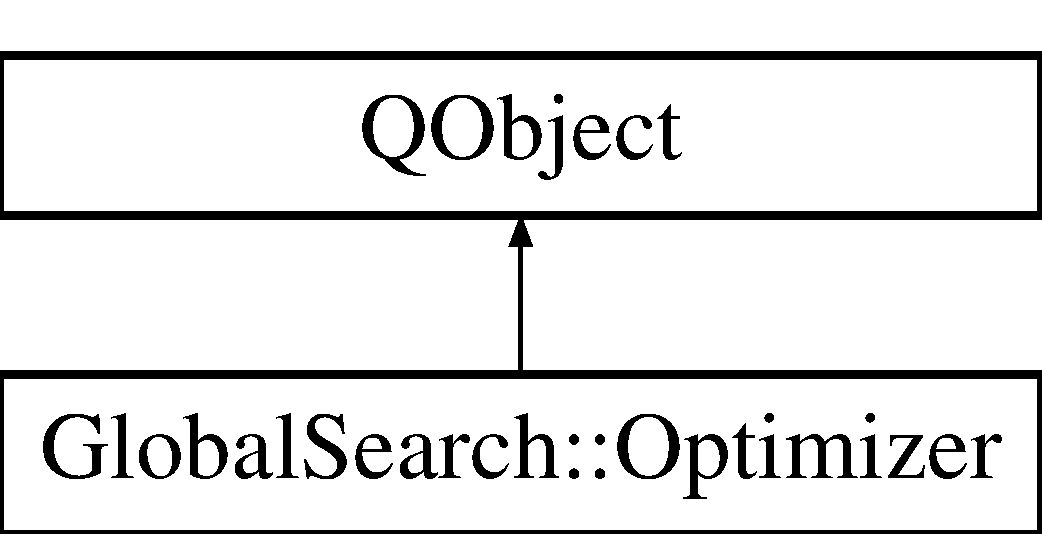
\includegraphics[height=2.000000cm]{classGlobalSearch_1_1Optimizer}
\end{center}
\end{figure}
\subsection*{Public Slots}
\begin{DoxyCompactItemize}
\item 
virtual bool \hyperlink{classGlobalSearch_1_1Optimizer_a83db0ac69c8b97825fc5d8361107ada4}{set\-Template} (const Q\-String \&filename, const Q\-String \&template\-Data, int opt\-Step\-Index)
\item 
virtual bool \hyperlink{classGlobalSearch_1_1Optimizer_ab4be28b4fc40d106ffa5ae1c9d67a6f3}{set\-Template} (const Q\-String \&filename, const Q\-String\-List \&template\-Data)
\item 
virtual bool \hyperlink{classGlobalSearch_1_1Optimizer_a8734827ff8773648cf4da48988208d87}{append\-Template} (const Q\-String \&filename, const Q\-String \&template\-Data)
\item 
virtual bool \hyperlink{classGlobalSearch_1_1Optimizer_a894c2cc508b92f2bb1678cc750faab30}{remove\-All\-Templates\-For\-Opt\-Step} (int opt\-Step\-Index)
\item 
virtual bool \hyperlink{classGlobalSearch_1_1Optimizer_a0bea17818fd8f29a13542119aebf2377}{set\-Data} (const Q\-String \&identifier, const Q\-Variant \&data)
\item 
void \hyperlink{classGlobalSearch_1_1Optimizer_adfb8a9de9d1eac7d5b188f6ae24c5ebc}{set\-User1} (const Q\-String \&s)
\item 
void \hyperlink{classGlobalSearch_1_1Optimizer_a9f53a4945abb35cda9a50fb973d27890}{set\-User2} (const Q\-String \&s)
\item 
void \hyperlink{classGlobalSearch_1_1Optimizer_a19e2d3e7c7a31f1ae94a3a58c0b3a6bf}{set\-User3} (const Q\-String \&s)
\item 
void \hyperlink{classGlobalSearch_1_1Optimizer_a713a94a031fc5fa7c653d54e6ef9fb64}{set\-User4} (const Q\-String \&s)
\item 
Q\-String \hyperlink{classGlobalSearch_1_1Optimizer_aed5eb285d45a001c9520c2ed3a5b57a1}{local\-Run\-Command} () const 
\item 
Q\-String \hyperlink{classGlobalSearch_1_1Optimizer_a5964a9b38d3ae90c8ac36a75d3a35832}{stdin\-Filename} () const 
\item 
Q\-String \hyperlink{classGlobalSearch_1_1Optimizer_a217750aa50431f9948aa8164fb99de0c}{stdout\-Filename} () const 
\item 
Q\-String \hyperlink{classGlobalSearch_1_1Optimizer_acaa83cc6bf1dcc263b92450b4f8cb652}{stderr\-Filename} () const 
\item 
virtual Q\-Hash$<$ Q\-String, Q\-String $>$ \hyperlink{classGlobalSearch_1_1Optimizer_aaaa0f0c28058c716fc065b48090c321f}{get\-Interpreted\-Templates} (\hyperlink{classGlobalSearch_1_1Structure}{Structure} $\ast$s)
\item 
bool \hyperlink{group__dialog_gac4335196cdf08e3555f6d0e152761604}{has\-Dialog} ()
\item 
virtual Q\-Dialog $\ast$ \hyperlink{group__dialog_ga9455d181accc40edd3ca6271fdc1e050}{dialog} ()
\end{DoxyCompactItemize}
\subsection*{Public Member Functions}
\begin{DoxyCompactItemize}
\item 
\hyperlink{classGlobalSearch_1_1Optimizer_a8c5a3335ff76f8a6a21a160d0139d842}{Optimizer} (\hyperlink{classGlobalSearch_1_1OptBase}{Opt\-Base} $\ast$parent, const Q\-String \&filename=\char`\"{}\char`\"{})
\item 
virtual \hyperlink{classGlobalSearch_1_1Optimizer_ace719aed9bbba0b3a568513ff68f8067}{$\sim$\-Optimizer} ()
\item 
virtual void \hyperlink{classGlobalSearch_1_1Optimizer_afef2dc22aa09df5e50e2f7b4f492091a}{read\-Settings} (const Q\-String \&filename=\char`\"{}\char`\"{})
\item 
virtual void \hyperlink{classGlobalSearch_1_1Optimizer_af67c36d87d7b41b1e91773b519d77829}{write\-Settings} (const Q\-String \&filename=\char`\"{}\char`\"{})
\item 
virtual Q\-String \hyperlink{classGlobalSearch_1_1Optimizer_aa81df016b0c8f3055a5e9e917eaefc75}{get\-I\-D\-String} ()
\item 
virtual int \hyperlink{classGlobalSearch_1_1Optimizer_aeeb18e38fa60535f74b577591400dd60}{get\-Number\-Of\-Opt\-Steps} ()
\item 
virtual bool \hyperlink{classGlobalSearch_1_1Optimizer_a10d37164307814e91c55bf846a59a80b}{is\-Ready\-To\-Search} (Q\-String $\ast$err)
\item 
virtual bool \hyperlink{classGlobalSearch_1_1Optimizer_afb5058a5e6a94e49c249284401680d5f}{check\-If\-Output\-File\-Exists} (\hyperlink{classGlobalSearch_1_1Structure}{Structure} $\ast$s, bool $\ast$exists)
\item 
virtual bool \hyperlink{classGlobalSearch_1_1Optimizer_a8d9373ded1b851ae6fdcbff41ed911cf}{check\-For\-Successful\-Output} (\hyperlink{classGlobalSearch_1_1Structure}{Structure} $\ast$s, bool $\ast$success)
\item 
virtual bool \hyperlink{classGlobalSearch_1_1Optimizer_a7e57844e4e6d713c87e6cf29ea03c5e2}{update} (\hyperlink{classGlobalSearch_1_1Structure}{Structure} $\ast$structure)
\item 
virtual bool \hyperlink{classGlobalSearch_1_1Optimizer_a5a2c5bc75be24ee41c27c1a2fe0e446a}{load} (\hyperlink{classGlobalSearch_1_1Structure}{Structure} $\ast$structure)
\item 
virtual bool \hyperlink{classGlobalSearch_1_1Optimizer_a671035cb8c0afbb4a1755b395bd063bd}{read} (\hyperlink{classGlobalSearch_1_1Structure}{Structure} $\ast$structure, const Q\-String \&filename)
\item 
virtual Q\-String \hyperlink{classGlobalSearch_1_1Optimizer_a739ab995b0a4cfcf8b9c8fd86e3a9f24}{get\-Template} (const Q\-String \&filename, int opt\-Step\-Index)
\item 
virtual Q\-String\-List \hyperlink{classGlobalSearch_1_1Optimizer_af46e4dd4e1e7dca1c3389fc8f30ea74e}{get\-Template} (const Q\-String \&filename)
\item 
virtual Q\-Variant \hyperlink{classGlobalSearch_1_1Optimizer_a512b302d7bc91999350ead624259a3cf}{get\-Data} (const Q\-String \&identifier)
\item 
virtual Q\-String\-List \hyperlink{classGlobalSearch_1_1Optimizer_a2819ce65995524d999c61b017192f77d}{get\-Template\-Names} ()
\item 
virtual Q\-String\-List \hyperlink{classGlobalSearch_1_1Optimizer_a4fb3da2a83d851f3ab53b8bc29026886}{get\-Data\-Identifiers} ()
\item 
Q\-String \hyperlink{classGlobalSearch_1_1Optimizer_a414f7b1587c6048451191bc915b640c5}{get\-User1} ()
\item 
Q\-String \hyperlink{classGlobalSearch_1_1Optimizer_a26166bc3bc6c3af4baa0e3f12ac41d38}{get\-User2} ()
\item 
Q\-String \hyperlink{classGlobalSearch_1_1Optimizer_a8b93a20caff4d31524283695f011ab85}{get\-User3} ()
\item 
Q\-String \hyperlink{classGlobalSearch_1_1Optimizer_a854917e1b3ba0bc164ab8edff823a3ae}{get\-User4} ()
\end{DoxyCompactItemize}
\subsection*{Protected Slots}
\begin{DoxyCompactItemize}
\item 
virtual void \hyperlink{classGlobalSearch_1_1Optimizer_ad9c1899c333b7aa692bfe7ff252a6222}{update\-Queue\-Interface} ()
\end{DoxyCompactItemize}
\subsection*{Protected Member Functions}
\begin{DoxyCompactItemize}
\item 
virtual void \hyperlink{classGlobalSearch_1_1Optimizer_a2e365a82ae293c91516270f5e6534960}{read\-Templates\-From\-Settings} (const Q\-String \&filename=\char`\"{}\char`\"{})
\item 
virtual void \hyperlink{classGlobalSearch_1_1Optimizer_a9c1a95c53dcdb90dce83be3ad07ac719}{write\-Templates\-To\-Settings} (const Q\-String \&filename=\char`\"{}\char`\"{})
\item 
virtual void \hyperlink{classGlobalSearch_1_1Optimizer_a5cc22352d86ce253a0aa8d9b2ee8c951}{read\-User\-Values\-From\-Settings} (const Q\-String \&filename=\char`\"{}\char`\"{})
\item 
virtual void \hyperlink{classGlobalSearch_1_1Optimizer_afa884a475b8001a43e592f466cf2318c}{write\-User\-Values\-To\-Settings} (const Q\-String \&filename=\char`\"{}\char`\"{})
\item 
virtual void \hyperlink{classGlobalSearch_1_1Optimizer_a17b4f7c9fd176d976d652598497ff70e}{read\-Data\-From\-Settings} (const Q\-String \&filename=\char`\"{}\char`\"{})
\item 
virtual void \hyperlink{classGlobalSearch_1_1Optimizer_a115e78eb651af3e0fbb9fe188d50ecdc}{write\-Data\-To\-Settings} (const Q\-String \&filename=\char`\"{}\char`\"{})
\item 
Q\-Hash$<$ Q\-String, Q\-String\-List $>$ \& \hyperlink{classGlobalSearch_1_1Optimizer_a56df447e7eab1eb64bd66f4e3bd4594d}{resolve\-Template\-Hash} (const Q\-String \&filename)
\item 
const Q\-Hash$<$ Q\-String, \\*
Q\-String\-List $>$ \& \hyperlink{classGlobalSearch_1_1Optimizer_a139e0f44d76b023c82e48149e595cbc5}{resolve\-Template\-Hash} (const Q\-String \&filename) const 
\item 
virtual void \hyperlink{classGlobalSearch_1_1Optimizer_a8205c1cb67d2111c0a9e13e78a543f00}{fix\-Template\-Lengths} ()
\end{DoxyCompactItemize}
\subsection*{Protected Attributes}
\begin{DoxyCompactItemize}
\item 
Q\-Hash$<$ Q\-String, Q\-Variant $>$ \hyperlink{classGlobalSearch_1_1Optimizer_a5cf732e34a6eaa4a7b1781d23e6e1c6e}{m\-\_\-data}
\item 
Q\-Hash$<$ Q\-String, Q\-String\-List $>$ \hyperlink{classGlobalSearch_1_1Optimizer_aa5892c64826b7cc7a2baa092efc8c66d}{m\-\_\-templates}
\item 
Q\-Hash$<$ Q\-String, Q\-String\-List $>$ \hyperlink{classGlobalSearch_1_1Optimizer_ac23d5114bf09b816666351868d49d1f8}{m\-\_\-\-Q\-I\-Templates}
\item 
Q\-String \hyperlink{classGlobalSearch_1_1Optimizer_a5e7a476823bc2d4b63939a9ada4f8ed0}{m\-\_\-completion\-Filename}
\item 
Q\-String\-List \hyperlink{classGlobalSearch_1_1Optimizer_a65ee33ee8778c366e8b197e75ae8e674}{m\-\_\-completion\-Strings}
\item 
Q\-String\-List \hyperlink{classGlobalSearch_1_1Optimizer_a28a8bf74bf7bdf00d453890796574c7d}{m\-\_\-output\-Filenames}
\item 
Q\-String \hyperlink{classGlobalSearch_1_1Optimizer_a1cdb6b6c5e929e84c834ba93148fb31e}{m\-\_\-local\-Run\-Command}
\item 
Q\-String \hyperlink{classGlobalSearch_1_1Optimizer_aca91d12d7aecae052d6ab5ae158acec6}{m\-\_\-stdin\-Filename}
\item 
Q\-String \hyperlink{classGlobalSearch_1_1Optimizer_a5ed04fdd5f8b511249e408adcd174550}{m\-\_\-stdout\-Filename}
\item 
Q\-String \hyperlink{classGlobalSearch_1_1Optimizer_a75b800a7f90a03d551f6795404d0c8f1}{m\-\_\-stderr\-Filename}
\item 
Q\-String \hyperlink{classGlobalSearch_1_1Optimizer_ae300aaecb74a7a61a501e4b8bd988957}{m\-\_\-user1}
\item 
Q\-String \hyperlink{classGlobalSearch_1_1Optimizer_a5ca1294d2a3aa119dfab655dfa270d3a}{m\-\_\-user2}
\item 
Q\-String \hyperlink{classGlobalSearch_1_1Optimizer_a279ca8ed61d6ca36f70c5c69b4d57397}{m\-\_\-user3}
\item 
Q\-String \hyperlink{classGlobalSearch_1_1Optimizer_aefab51b84978d2fb49eaf3585894808a}{m\-\_\-user4}
\item 
\hyperlink{classGlobalSearch_1_1OptBase}{Opt\-Base} $\ast$ \hyperlink{classGlobalSearch_1_1Optimizer_a689df6e2c0d8bbfff99585ca54199696}{m\-\_\-opt}
\item 
Q\-String \hyperlink{classGlobalSearch_1_1Optimizer_a4d2dc8b7aaa3bb6fed8c28547460def8}{m\-\_\-id\-String}
\end{DoxyCompactItemize}
\subsection*{Friends}
\begin{DoxyCompactItemize}
\item 
\hypertarget{classGlobalSearch_1_1Optimizer_a820134b906cccccfc214c45661db99bf}{class {\bfseries Optimizer\-Config\-Dialog}}\label{classGlobalSearch_1_1Optimizer_a820134b906cccccfc214c45661db99bf}

\end{DoxyCompactItemize}


\subsection{Detailed Description}
The \hyperlink{classGlobalSearch_1_1Optimizer}{Optimizer} class provides an interface between an \hyperlink{classGlobalSearch_1_1OptBase}{Opt\-Base} instance and an external optimization engine. 

\begin{DoxyAuthor}{Author}
David C. Lonie
\end{DoxyAuthor}
The \hyperlink{classGlobalSearch_1_1Optimizer}{Optimizer} class standardizes communication between an \hyperlink{classGlobalSearch_1_1OptBase}{Opt\-Base} instance and an external chemical optimization engine, such as G\-A\-M\-E\-S\-S, A\-D\-F, V\-A\-S\-P, etc.

The file contents may be set using the set\-Template, append\-Template, and remove\-Template functions. These will be passed through the associated \hyperlink{classGlobalSearch_1_1OptBase}{Opt\-Base}'s template interpreter prior to writing.

Once the \hyperlink{classGlobalSearch_1_1Optimizer}{Optimizer} is attached to the \hyperlink{classGlobalSearch_1_1OptBase}{Opt\-Base} instance and the templates are set, the \hyperlink{classGlobalSearch_1_1QueueManager}{Queue\-Manager} handles all job submission, file writing, and \hyperlink{classGlobalSearch_1_1Structure}{Structure} updating automatically. 

Definition at line 52 of file optimizer.\-h.



\subsection{Constructor \& Destructor Documentation}
\hypertarget{classGlobalSearch_1_1Optimizer_a8c5a3335ff76f8a6a21a160d0139d842}{\index{Global\-Search\-::\-Optimizer@{Global\-Search\-::\-Optimizer}!Optimizer@{Optimizer}}
\index{Optimizer@{Optimizer}!GlobalSearch::Optimizer@{Global\-Search\-::\-Optimizer}}
\subsubsection[{Optimizer}]{\setlength{\rightskip}{0pt plus 5cm}Global\-Search\-::\-Optimizer\-::\-Optimizer (
\begin{DoxyParamCaption}
\item[{{\bf Opt\-Base} $\ast$}]{parent, }
\item[{const Q\-String \&}]{filename = {\ttfamily \char`\"{}\char`\"{}}}
\end{DoxyParamCaption}
)\hspace{0.3cm}{\ttfamily [explicit]}}}\label{classGlobalSearch_1_1Optimizer_a8c5a3335ff76f8a6a21a160d0139d842}
Constructor


\begin{DoxyParams}{Parameters}
{\em parent} & \hyperlink{classGlobalSearch_1_1OptBase}{Opt\-Base} parent \\
\hline
{\em filename} & Optional filename to load data from (scheme or resume file) \\
\hline
\end{DoxyParams}


Definition at line 41 of file optimizer.\-cpp.



References m\-\_\-id\-String, m\-\_\-opt, m\-\_\-stderr\-Filename, m\-\_\-stdin\-Filename, m\-\_\-stdout\-Filename, Global\-Search\-::\-Opt\-Base\-::queue\-Interface(), read\-Settings(), and update\-Queue\-Interface().

\hypertarget{classGlobalSearch_1_1Optimizer_ace719aed9bbba0b3a568513ff68f8067}{\index{Global\-Search\-::\-Optimizer@{Global\-Search\-::\-Optimizer}!$\sim$\-Optimizer@{$\sim$\-Optimizer}}
\index{$\sim$\-Optimizer@{$\sim$\-Optimizer}!GlobalSearch::Optimizer@{Global\-Search\-::\-Optimizer}}
\subsubsection[{$\sim$\-Optimizer}]{\setlength{\rightskip}{0pt plus 5cm}Global\-Search\-::\-Optimizer\-::$\sim$\-Optimizer (
\begin{DoxyParamCaption}
{}
\end{DoxyParamCaption}
)\hspace{0.3cm}{\ttfamily [virtual]}}}\label{classGlobalSearch_1_1Optimizer_ace719aed9bbba0b3a568513ff68f8067}
Destructor 

Definition at line 107 of file optimizer.\-cpp.



\subsection{Member Function Documentation}
\hypertarget{classGlobalSearch_1_1Optimizer_a8734827ff8773648cf4da48988208d87}{\index{Global\-Search\-::\-Optimizer@{Global\-Search\-::\-Optimizer}!append\-Template@{append\-Template}}
\index{append\-Template@{append\-Template}!GlobalSearch::Optimizer@{Global\-Search\-::\-Optimizer}}
\subsubsection[{append\-Template}]{\setlength{\rightskip}{0pt plus 5cm}bool Global\-Search\-::\-Optimizer\-::append\-Template (
\begin{DoxyParamCaption}
\item[{const Q\-String \&}]{filename, }
\item[{const Q\-String \&}]{template\-Data}
\end{DoxyParamCaption}
)\hspace{0.3cm}{\ttfamily [virtual]}, {\ttfamily [slot]}}}\label{classGlobalSearch_1_1Optimizer_a8734827ff8773648cf4da48988208d87}
Add a new optimization step for a given filename.


\begin{DoxyParams}{Parameters}
{\em filename} & Filename identifying the template \\
\hline
{\em template\-Data} & Template string of the new optimization step.\\
\hline
\end{DoxyParams}
\begin{DoxyReturn}{Returns}
True if successful, false otherwise. 
\end{DoxyReturn}


Definition at line 583 of file optimizer.\-cpp.



References m\-\_\-\-Q\-I\-Templates, m\-\_\-templates, and resolve\-Template\-Hash().

\hypertarget{classGlobalSearch_1_1Optimizer_a8d9373ded1b851ae6fdcbff41ed911cf}{\index{Global\-Search\-::\-Optimizer@{Global\-Search\-::\-Optimizer}!check\-For\-Successful\-Output@{check\-For\-Successful\-Output}}
\index{check\-For\-Successful\-Output@{check\-For\-Successful\-Output}!GlobalSearch::Optimizer@{Global\-Search\-::\-Optimizer}}
\subsubsection[{check\-For\-Successful\-Output}]{\setlength{\rightskip}{0pt plus 5cm}bool Global\-Search\-::\-Optimizer\-::check\-For\-Successful\-Output (
\begin{DoxyParamCaption}
\item[{{\bf Structure} $\ast$}]{s, }
\item[{bool $\ast$}]{success}
\end{DoxyParamCaption}
)\hspace{0.3cm}{\ttfamily [virtual]}}}\label{classGlobalSearch_1_1Optimizer_a8d9373ded1b851ae6fdcbff41ed911cf}
Check m\-\_\-completion\-Filename for any of the m\-\_\-completion\-Strings in the working directory of \hyperlink{classGlobalSearch_1_1Structure}{Structure} {\itshape s}. If any are found, {\itshape success} is set to true.

\begin{DoxyNote}{Note}
This function uses the argument {\itshape success} to report whether or not m\-\_\-completion\-File\-Name contains any m\-\_\-completion\-Strings. The return value indicates whether the file check was performed without errors (e.\-g. network errors).
\end{DoxyNote}
\begin{DoxyReturn}{Returns}
True if the test encountered no errors, false otherwise. 
\end{DoxyReturn}


Definition at line 369 of file optimizer.\-cpp.



References Global\-Search\-::\-Queue\-Interface\-::grep\-File(), m\-\_\-completion\-Filename, m\-\_\-completion\-Strings, m\-\_\-opt, and Global\-Search\-::\-Opt\-Base\-::queue\-Interface().



Referenced by Global\-Search\-::\-Local\-Queue\-Interface\-::get\-Status().

\hypertarget{classGlobalSearch_1_1Optimizer_afb5058a5e6a94e49c249284401680d5f}{\index{Global\-Search\-::\-Optimizer@{Global\-Search\-::\-Optimizer}!check\-If\-Output\-File\-Exists@{check\-If\-Output\-File\-Exists}}
\index{check\-If\-Output\-File\-Exists@{check\-If\-Output\-File\-Exists}!GlobalSearch::Optimizer@{Global\-Search\-::\-Optimizer}}
\subsubsection[{check\-If\-Output\-File\-Exists}]{\setlength{\rightskip}{0pt plus 5cm}bool Global\-Search\-::\-Optimizer\-::check\-If\-Output\-File\-Exists (
\begin{DoxyParamCaption}
\item[{{\bf Structure} $\ast$}]{s, }
\item[{bool $\ast$}]{exists}
\end{DoxyParamCaption}
)\hspace{0.3cm}{\ttfamily [virtual]}}}\label{classGlobalSearch_1_1Optimizer_afb5058a5e6a94e49c249284401680d5f}
Check if the file m\-\_\-completion\-Filename exists in the working directory of \hyperlink{classGlobalSearch_1_1Structure}{Structure} {\itshape s} and store the result in {\itshape exists}.

\begin{DoxyNote}{Note}
This function uses the argument {\itshape exists} to report whether or not the file exists. The return value indicates whether the file check was performed without errors (e.\-g. network errors).
\end{DoxyNote}
\begin{DoxyReturn}{Returns}
True if the test encountered no errors, false otherwise. 
\end{DoxyReturn}


Definition at line 362 of file optimizer.\-cpp.



References Global\-Search\-::\-Queue\-Interface\-::check\-If\-File\-Exists(), m\-\_\-completion\-Filename, m\-\_\-opt, and Global\-Search\-::\-Opt\-Base\-::queue\-Interface().



Referenced by Global\-Search\-::\-Local\-Queue\-Interface\-::get\-Status().

\hypertarget{classGlobalSearch_1_1Optimizer_a8205c1cb67d2111c0a9e13e78a543f00}{\index{Global\-Search\-::\-Optimizer@{Global\-Search\-::\-Optimizer}!fix\-Template\-Lengths@{fix\-Template\-Lengths}}
\index{fix\-Template\-Lengths@{fix\-Template\-Lengths}!GlobalSearch::Optimizer@{Global\-Search\-::\-Optimizer}}
\subsubsection[{fix\-Template\-Lengths}]{\setlength{\rightskip}{0pt plus 5cm}void Global\-Search\-::\-Optimizer\-::fix\-Template\-Lengths (
\begin{DoxyParamCaption}
{}
\end{DoxyParamCaption}
)\hspace{0.3cm}{\ttfamily [protected]}, {\ttfamily [virtual]}}}\label{classGlobalSearch_1_1Optimizer_a8205c1cb67d2111c0a9e13e78a543f00}
Ensure that all template lists in m\-\_\-templates and m\-\_\-\-Q\-I\-Templates contain \hyperlink{classGlobalSearch_1_1Optimizer_aeeb18e38fa60535f74b577591400dd60}{get\-Number\-Of\-Opt\-Steps()} optimization steps.

If a template list has too few entries, empty strings are appended. 

Definition at line 672 of file optimizer.\-cpp.



References get\-Number\-Of\-Opt\-Steps(), m\-\_\-\-Q\-I\-Templates, and m\-\_\-templates.



Referenced by read\-Templates\-From\-Settings().

\hypertarget{classGlobalSearch_1_1Optimizer_a512b302d7bc91999350ead624259a3cf}{\index{Global\-Search\-::\-Optimizer@{Global\-Search\-::\-Optimizer}!get\-Data@{get\-Data}}
\index{get\-Data@{get\-Data}!GlobalSearch::Optimizer@{Global\-Search\-::\-Optimizer}}
\subsubsection[{get\-Data}]{\setlength{\rightskip}{0pt plus 5cm}Q\-Variant Global\-Search\-::\-Optimizer\-::get\-Data (
\begin{DoxyParamCaption}
\item[{const Q\-String \&}]{identifier}
\end{DoxyParamCaption}
)\hspace{0.3cm}{\ttfamily [virtual]}}}\label{classGlobalSearch_1_1Optimizer_a512b302d7bc91999350ead624259a3cf}
Get generic data associated with the optimizer.


\begin{DoxyParams}{Parameters}
{\em identifier} & Q\-String identifying the data needed.\\
\hline
\end{DoxyParams}
\begin{DoxyReturn}{Returns}
A Q\-Variant version of the generic data. 
\end{DoxyReturn}


Definition at line 625 of file optimizer.\-cpp.



References m\-\_\-data.

\hypertarget{classGlobalSearch_1_1Optimizer_a4fb3da2a83d851f3ab53b8bc29026886}{\index{Global\-Search\-::\-Optimizer@{Global\-Search\-::\-Optimizer}!get\-Data\-Identifiers@{get\-Data\-Identifiers}}
\index{get\-Data\-Identifiers@{get\-Data\-Identifiers}!GlobalSearch::Optimizer@{Global\-Search\-::\-Optimizer}}
\subsubsection[{get\-Data\-Identifiers}]{\setlength{\rightskip}{0pt plus 5cm}virtual Q\-String\-List Global\-Search\-::\-Optimizer\-::get\-Data\-Identifiers (
\begin{DoxyParamCaption}
{}
\end{DoxyParamCaption}
)\hspace{0.3cm}{\ttfamily [inline]}, {\ttfamily [virtual]}}}\label{classGlobalSearch_1_1Optimizer_a4fb3da2a83d851f3ab53b8bc29026886}
\begin{DoxyReturn}{Returns}
All strings that identify valid generic data sets. 
\end{DoxyReturn}


Definition at line 217 of file optimizer.\-h.



References m\-\_\-data.



Referenced by read\-Data\-From\-Settings(), and write\-Data\-To\-Settings().

\hypertarget{classGlobalSearch_1_1Optimizer_aa81df016b0c8f3055a5e9e917eaefc75}{\index{Global\-Search\-::\-Optimizer@{Global\-Search\-::\-Optimizer}!get\-I\-D\-String@{get\-I\-D\-String}}
\index{get\-I\-D\-String@{get\-I\-D\-String}!GlobalSearch::Optimizer@{Global\-Search\-::\-Optimizer}}
\subsubsection[{get\-I\-D\-String}]{\setlength{\rightskip}{0pt plus 5cm}virtual Q\-String Global\-Search\-::\-Optimizer\-::get\-I\-D\-String (
\begin{DoxyParamCaption}
{}
\end{DoxyParamCaption}
)\hspace{0.3cm}{\ttfamily [inline]}, {\ttfamily [virtual]}}}\label{classGlobalSearch_1_1Optimizer_aa81df016b0c8f3055a5e9e917eaefc75}
\begin{DoxyReturn}{Returns}
A string identifying the \hyperlink{classGlobalSearch_1_1Optimizer}{Optimizer} 
\end{DoxyReturn}


Definition at line 96 of file optimizer.\-h.



References m\-\_\-id\-String.



Referenced by read\-Data\-From\-Settings(), read\-Templates\-From\-Settings(), read\-User\-Values\-From\-Settings(), Global\-Search\-::\-Abstract\-Edit\-Tab\-::save\-Scheme(), write\-Data\-To\-Settings(), write\-Templates\-To\-Settings(), and write\-User\-Values\-To\-Settings().

\hypertarget{classGlobalSearch_1_1Optimizer_aaaa0f0c28058c716fc065b48090c321f}{\index{Global\-Search\-::\-Optimizer@{Global\-Search\-::\-Optimizer}!get\-Interpreted\-Templates@{get\-Interpreted\-Templates}}
\index{get\-Interpreted\-Templates@{get\-Interpreted\-Templates}!GlobalSearch::Optimizer@{Global\-Search\-::\-Optimizer}}
\subsubsection[{get\-Interpreted\-Templates}]{\setlength{\rightskip}{0pt plus 5cm}Q\-Hash$<$ Q\-String, Q\-String $>$ Global\-Search\-::\-Optimizer\-::get\-Interpreted\-Templates (
\begin{DoxyParamCaption}
\item[{{\bf Structure} $\ast$}]{s}
\end{DoxyParamCaption}
)\hspace{0.3cm}{\ttfamily [virtual]}, {\ttfamily [slot]}}}\label{classGlobalSearch_1_1Optimizer_aaaa0f0c28058c716fc065b48090c321f}
Interpret all templates in m\-\_\-templates at the \hyperlink{classGlobalSearch_1_1Structure}{Structure}'s current optimization step.


\begin{DoxyParams}{Parameters}
{\em s} & \hyperlink{classGlobalSearch_1_1Structure}{Structure} of interest\\
\hline
\end{DoxyParams}
\begin{DoxyReturn}{Returns}
A hash containing the interpreted templates, key\-: filename, value\-: file contents 
\end{DoxyReturn}


Definition at line 281 of file optimizer.\-cpp.



References Global\-Search\-::\-Structure\-::get\-Current\-Opt\-Step(), Global\-Search\-::\-Structure\-::get\-I\-D\-String(), get\-Number\-Of\-Opt\-Steps(), Global\-Search\-::\-Opt\-Base\-::interpret\-Template(), m\-\_\-opt, m\-\_\-\-Q\-I\-Templates, m\-\_\-templates, Global\-Search\-::\-Opt\-Base\-::optimizer(), Global\-Search\-::\-Opt\-Base\-::queue\-Interface(), and Global\-Search\-::\-Queue\-Interface\-::stop\-Job().



Referenced by Global\-Search\-::\-Queue\-Interface\-::write\-Input\-Files().

\hypertarget{classGlobalSearch_1_1Optimizer_aeeb18e38fa60535f74b577591400dd60}{\index{Global\-Search\-::\-Optimizer@{Global\-Search\-::\-Optimizer}!get\-Number\-Of\-Opt\-Steps@{get\-Number\-Of\-Opt\-Steps}}
\index{get\-Number\-Of\-Opt\-Steps@{get\-Number\-Of\-Opt\-Steps}!GlobalSearch::Optimizer@{Global\-Search\-::\-Optimizer}}
\subsubsection[{get\-Number\-Of\-Opt\-Steps}]{\setlength{\rightskip}{0pt plus 5cm}int Global\-Search\-::\-Optimizer\-::get\-Number\-Of\-Opt\-Steps (
\begin{DoxyParamCaption}
{}
\end{DoxyParamCaption}
)\hspace{0.3cm}{\ttfamily [virtual]}}}\label{classGlobalSearch_1_1Optimizer_aeeb18e38fa60535f74b577591400dd60}
\begin{DoxyReturn}{Returns}
The total number of optimization steps 
\end{DoxyReturn}


Definition at line 535 of file optimizer.\-cpp.



References m\-\_\-templates.



Referenced by Global\-Search\-::\-Abstract\-Edit\-Tab\-::append\-Opt\-Step(), fix\-Template\-Lengths(), get\-Interpreted\-Templates(), get\-Template(), Global\-Search\-::\-Abstract\-Edit\-Tab\-::populate\-Opt\-Step\-List(), remove\-All\-Templates\-For\-Opt\-Step(), Global\-Search\-::\-Abstract\-Edit\-Tab\-::remove\-Current\-Opt\-Step(), Global\-Search\-::\-Abstract\-Edit\-Tab\-::save\-Current\-Template(), set\-Template(), Global\-Search\-::\-Abstract\-Edit\-Tab\-::update\-Edit\-Widget(), and update\-Queue\-Interface().

\hypertarget{classGlobalSearch_1_1Optimizer_a739ab995b0a4cfcf8b9c8fd86e3a9f24}{\index{Global\-Search\-::\-Optimizer@{Global\-Search\-::\-Optimizer}!get\-Template@{get\-Template}}
\index{get\-Template@{get\-Template}!GlobalSearch::Optimizer@{Global\-Search\-::\-Optimizer}}
\subsubsection[{get\-Template}]{\setlength{\rightskip}{0pt plus 5cm}Q\-String Global\-Search\-::\-Optimizer\-::get\-Template (
\begin{DoxyParamCaption}
\item[{const Q\-String \&}]{filename, }
\item[{int}]{opt\-Step\-Index}
\end{DoxyParamCaption}
)\hspace{0.3cm}{\ttfamily [virtual]}}}\label{classGlobalSearch_1_1Optimizer_a739ab995b0a4cfcf8b9c8fd86e3a9f24}
Return a specified template.


\begin{DoxyParams}{Parameters}
{\em filename} & Filename of template \\
\hline
{\em opt\-Step\-Index} & Optimization step index of template to retrieve.\\
\hline
\end{DoxyParams}
\begin{DoxyReturn}{Returns}
The requested template 
\end{DoxyReturn}


Definition at line 565 of file optimizer.\-cpp.



References get\-Number\-Of\-Opt\-Steps(), m\-\_\-\-Q\-I\-Templates, m\-\_\-templates, and resolve\-Template\-Hash().



Referenced by Global\-Search\-::\-Abstract\-Edit\-Tab\-::update\-Edit\-Widget().

\hypertarget{classGlobalSearch_1_1Optimizer_af46e4dd4e1e7dca1c3389fc8f30ea74e}{\index{Global\-Search\-::\-Optimizer@{Global\-Search\-::\-Optimizer}!get\-Template@{get\-Template}}
\index{get\-Template@{get\-Template}!GlobalSearch::Optimizer@{Global\-Search\-::\-Optimizer}}
\subsubsection[{get\-Template}]{\setlength{\rightskip}{0pt plus 5cm}Q\-String\-List Global\-Search\-::\-Optimizer\-::get\-Template (
\begin{DoxyParamCaption}
\item[{const Q\-String \&}]{filename}
\end{DoxyParamCaption}
)\hspace{0.3cm}{\ttfamily [virtual]}}}\label{classGlobalSearch_1_1Optimizer_af46e4dd4e1e7dca1c3389fc8f30ea74e}
Return a list of all templates for a given filename


\begin{DoxyParams}{Parameters}
{\em filename} & Filename of template\\
\hline
\end{DoxyParams}
\begin{DoxyReturn}{Returns}
A list of all template matching the given filename, in order of optimization step. 
\end{DoxyReturn}


Definition at line 575 of file optimizer.\-cpp.



References m\-\_\-\-Q\-I\-Templates, m\-\_\-templates, and resolve\-Template\-Hash().

\hypertarget{classGlobalSearch_1_1Optimizer_a2819ce65995524d999c61b017192f77d}{\index{Global\-Search\-::\-Optimizer@{Global\-Search\-::\-Optimizer}!get\-Template\-Names@{get\-Template\-Names}}
\index{get\-Template\-Names@{get\-Template\-Names}!GlobalSearch::Optimizer@{Global\-Search\-::\-Optimizer}}
\subsubsection[{get\-Template\-Names}]{\setlength{\rightskip}{0pt plus 5cm}virtual Q\-String\-List Global\-Search\-::\-Optimizer\-::get\-Template\-Names (
\begin{DoxyParamCaption}
{}
\end{DoxyParamCaption}
)\hspace{0.3cm}{\ttfamily [inline]}, {\ttfamily [virtual]}}}\label{classGlobalSearch_1_1Optimizer_a2819ce65995524d999c61b017192f77d}
\begin{DoxyReturn}{Returns}
All filenames that the optimizer can store templates for. 
\end{DoxyReturn}


Definition at line 212 of file optimizer.\-h.



References m\-\_\-templates.



Referenced by Global\-Search\-::\-Abstract\-Edit\-Tab\-::get\-Template\-Names(), read\-Templates\-From\-Settings(), and write\-Templates\-To\-Settings().

\hypertarget{classGlobalSearch_1_1Optimizer_a414f7b1587c6048451191bc915b640c5}{\index{Global\-Search\-::\-Optimizer@{Global\-Search\-::\-Optimizer}!get\-User1@{get\-User1}}
\index{get\-User1@{get\-User1}!GlobalSearch::Optimizer@{Global\-Search\-::\-Optimizer}}
\subsubsection[{get\-User1}]{\setlength{\rightskip}{0pt plus 5cm}Q\-String Global\-Search\-::\-Optimizer\-::get\-User1 (
\begin{DoxyParamCaption}
{}
\end{DoxyParamCaption}
)\hspace{0.3cm}{\ttfamily [inline]}}}\label{classGlobalSearch_1_1Optimizer_a414f7b1587c6048451191bc915b640c5}
\begin{DoxyReturn}{Returns}
A user customizable string that is used in template interpretation. 
\end{DoxyReturn}


Definition at line 223 of file optimizer.\-h.



References m\-\_\-user1.



Referenced by Global\-Search\-::\-Opt\-Base\-::interpret\-Keyword\-\_\-base(), and Global\-Search\-::\-Abstract\-Edit\-Tab\-::update\-G\-U\-I().

\hypertarget{classGlobalSearch_1_1Optimizer_a26166bc3bc6c3af4baa0e3f12ac41d38}{\index{Global\-Search\-::\-Optimizer@{Global\-Search\-::\-Optimizer}!get\-User2@{get\-User2}}
\index{get\-User2@{get\-User2}!GlobalSearch::Optimizer@{Global\-Search\-::\-Optimizer}}
\subsubsection[{get\-User2}]{\setlength{\rightskip}{0pt plus 5cm}Q\-String Global\-Search\-::\-Optimizer\-::get\-User2 (
\begin{DoxyParamCaption}
{}
\end{DoxyParamCaption}
)\hspace{0.3cm}{\ttfamily [inline]}}}\label{classGlobalSearch_1_1Optimizer_a26166bc3bc6c3af4baa0e3f12ac41d38}
\begin{DoxyReturn}{Returns}
A user customizable string that is used in template interpretation. 
\end{DoxyReturn}


Definition at line 229 of file optimizer.\-h.



References m\-\_\-user2.



Referenced by Global\-Search\-::\-Opt\-Base\-::interpret\-Keyword\-\_\-base(), and Global\-Search\-::\-Abstract\-Edit\-Tab\-::update\-G\-U\-I().

\hypertarget{classGlobalSearch_1_1Optimizer_a8b93a20caff4d31524283695f011ab85}{\index{Global\-Search\-::\-Optimizer@{Global\-Search\-::\-Optimizer}!get\-User3@{get\-User3}}
\index{get\-User3@{get\-User3}!GlobalSearch::Optimizer@{Global\-Search\-::\-Optimizer}}
\subsubsection[{get\-User3}]{\setlength{\rightskip}{0pt plus 5cm}Q\-String Global\-Search\-::\-Optimizer\-::get\-User3 (
\begin{DoxyParamCaption}
{}
\end{DoxyParamCaption}
)\hspace{0.3cm}{\ttfamily [inline]}}}\label{classGlobalSearch_1_1Optimizer_a8b93a20caff4d31524283695f011ab85}
\begin{DoxyReturn}{Returns}
A user customizable string that is used in template interpretation. 
\end{DoxyReturn}


Definition at line 235 of file optimizer.\-h.



References m\-\_\-user3.



Referenced by Global\-Search\-::\-Opt\-Base\-::interpret\-Keyword\-\_\-base(), and Global\-Search\-::\-Abstract\-Edit\-Tab\-::update\-G\-U\-I().

\hypertarget{classGlobalSearch_1_1Optimizer_a854917e1b3ba0bc164ab8edff823a3ae}{\index{Global\-Search\-::\-Optimizer@{Global\-Search\-::\-Optimizer}!get\-User4@{get\-User4}}
\index{get\-User4@{get\-User4}!GlobalSearch::Optimizer@{Global\-Search\-::\-Optimizer}}
\subsubsection[{get\-User4}]{\setlength{\rightskip}{0pt plus 5cm}Q\-String Global\-Search\-::\-Optimizer\-::get\-User4 (
\begin{DoxyParamCaption}
{}
\end{DoxyParamCaption}
)\hspace{0.3cm}{\ttfamily [inline]}}}\label{classGlobalSearch_1_1Optimizer_a854917e1b3ba0bc164ab8edff823a3ae}
\begin{DoxyReturn}{Returns}
A user customizable string that is used in template interpretation. 
\end{DoxyReturn}


Definition at line 241 of file optimizer.\-h.



References m\-\_\-user4.



Referenced by Global\-Search\-::\-Opt\-Base\-::interpret\-Keyword\-\_\-base(), and Global\-Search\-::\-Abstract\-Edit\-Tab\-::update\-G\-U\-I().

\hypertarget{classGlobalSearch_1_1Optimizer_a10d37164307814e91c55bf846a59a80b}{\index{Global\-Search\-::\-Optimizer@{Global\-Search\-::\-Optimizer}!is\-Ready\-To\-Search@{is\-Ready\-To\-Search}}
\index{is\-Ready\-To\-Search@{is\-Ready\-To\-Search}!GlobalSearch::Optimizer@{Global\-Search\-::\-Optimizer}}
\subsubsection[{is\-Ready\-To\-Search}]{\setlength{\rightskip}{0pt plus 5cm}virtual bool Global\-Search\-::\-Optimizer\-::is\-Ready\-To\-Search (
\begin{DoxyParamCaption}
\item[{Q\-String $\ast$}]{err}
\end{DoxyParamCaption}
)\hspace{0.3cm}{\ttfamily [inline]}, {\ttfamily [virtual]}}}\label{classGlobalSearch_1_1Optimizer_a10d37164307814e91c55bf846a59a80b}
Check that all mandatory internal variables are set. Check this before starting a search.


\begin{DoxyParams}{Parameters}
{\em err} & String to be overwritten with an error message\\
\hline
\end{DoxyParams}
\begin{DoxyReturn}{Returns}
true if all variables are initialized, false otherwise. If false, {\itshape err} will be overwritten with a user-\/friendly error message. 
\end{DoxyReturn}


Definition at line 113 of file optimizer.\-h.

\hypertarget{classGlobalSearch_1_1Optimizer_a5a2c5bc75be24ee41c27c1a2fe0e446a}{\index{Global\-Search\-::\-Optimizer@{Global\-Search\-::\-Optimizer}!load@{load}}
\index{load@{load}!GlobalSearch::Optimizer@{Global\-Search\-::\-Optimizer}}
\subsubsection[{load}]{\setlength{\rightskip}{0pt plus 5cm}bool Global\-Search\-::\-Optimizer\-::load (
\begin{DoxyParamCaption}
\item[{{\bf Structure} $\ast$}]{structure}
\end{DoxyParamCaption}
)\hspace{0.3cm}{\ttfamily [virtual]}}}\label{classGlobalSearch_1_1Optimizer_a5a2c5bc75be24ee41c27c1a2fe0e446a}
Update the \hyperlink{classGlobalSearch_1_1Structure}{Structure} from the files in the \hyperlink{classGlobalSearch_1_1Structure}{Structure}'s local file path.


\begin{DoxyParams}{Parameters}
{\em structure} & \hyperlink{classGlobalSearch_1_1Structure}{Structure} to be updated.\\
\hline
\end{DoxyParams}
\begin{DoxyReturn}{Returns}
True if successful, false otherwise. 
\end{DoxyReturn}
\begin{DoxySeeAlso}{See Also}
\hyperlink{classGlobalSearch_1_1Optimizer_a7e57844e4e6d713c87e6cf29ea03c5e2}{update} 

\hyperlink{classGlobalSearch_1_1Optimizer_a671035cb8c0afbb4a1755b395bd063bd}{read} 
\end{DoxySeeAlso}


Definition at line 430 of file optimizer.\-cpp.



References m\-\_\-opt, m\-\_\-output\-Filenames, read(), and Global\-Search\-::\-Opt\-Base\-::warning().

\hypertarget{classGlobalSearch_1_1Optimizer_aed5eb285d45a001c9520c2ed3a5b57a1}{\index{Global\-Search\-::\-Optimizer@{Global\-Search\-::\-Optimizer}!local\-Run\-Command@{local\-Run\-Command}}
\index{local\-Run\-Command@{local\-Run\-Command}!GlobalSearch::Optimizer@{Global\-Search\-::\-Optimizer}}
\subsubsection[{local\-Run\-Command}]{\setlength{\rightskip}{0pt plus 5cm}Q\-String Global\-Search\-::\-Optimizer\-::local\-Run\-Command (
\begin{DoxyParamCaption}
{}
\end{DoxyParamCaption}
) const\hspace{0.3cm}{\ttfamily [inline]}, {\ttfamily [slot]}}}\label{classGlobalSearch_1_1Optimizer_aed5eb285d45a001c9520c2ed3a5b57a1}
Command line used in local execution

Details given in m\-\_\-local\-Run\-Command.

\begin{DoxySeeAlso}{See Also}
\hyperlink{classGlobalSearch_1_1Optimizer_a5964a9b38d3ae90c8ac36a75d3a35832}{stdin\-Filename} 

\hyperlink{classGlobalSearch_1_1Optimizer_a217750aa50431f9948aa8164fb99de0c}{stdout\-Filename} 

\hyperlink{classGlobalSearch_1_1Optimizer_acaa83cc6bf1dcc263b92450b4f8cb652}{stderr\-Filename} 

\hyperlink{classGlobalSearch_1_1Optimizer_a1cdb6b6c5e929e84c834ba93148fb31e}{m\-\_\-local\-Run\-Command} 

\hyperlink{classGlobalSearch_1_1Optimizer_aca91d12d7aecae052d6ab5ae158acec6}{m\-\_\-stdin\-Filename} 

\hyperlink{classGlobalSearch_1_1Optimizer_a5ed04fdd5f8b511249e408adcd174550}{m\-\_\-stdout\-Filename} 

\hyperlink{classGlobalSearch_1_1Optimizer_a75b800a7f90a03d551f6795404d0c8f1}{m\-\_\-stderr\-Filename} 
\end{DoxySeeAlso}


Definition at line 344 of file optimizer.\-h.



References m\-\_\-local\-Run\-Command.



Referenced by Global\-Search\-::\-Local\-Queue\-Interface\-::start\-Job().

\hypertarget{classGlobalSearch_1_1Optimizer_a671035cb8c0afbb4a1755b395bd063bd}{\index{Global\-Search\-::\-Optimizer@{Global\-Search\-::\-Optimizer}!read@{read}}
\index{read@{read}!GlobalSearch::Optimizer@{Global\-Search\-::\-Optimizer}}
\subsubsection[{read}]{\setlength{\rightskip}{0pt plus 5cm}bool Global\-Search\-::\-Optimizer\-::read (
\begin{DoxyParamCaption}
\item[{{\bf Structure} $\ast$}]{structure, }
\item[{const Q\-String \&}]{filename}
\end{DoxyParamCaption}
)\hspace{0.3cm}{\ttfamily [virtual]}}}\label{classGlobalSearch_1_1Optimizer_a671035cb8c0afbb4a1755b395bd063bd}
Update the \hyperlink{classGlobalSearch_1_1Structure}{Structure} from the specified filename.


\begin{DoxyParams}{Parameters}
{\em structure} & \hyperlink{classGlobalSearch_1_1Structure}{Structure} to be updated \\
\hline
{\em filename} & Filename to read\\
\hline
\end{DoxyParams}
\begin{DoxyReturn}{Returns}
True if successful, false otherwise. 
\end{DoxyReturn}
\begin{DoxySeeAlso}{See Also}
\hyperlink{classGlobalSearch_1_1Optimizer_a7e57844e4e6d713c87e6cf29ea03c5e2}{update} 

\hyperlink{classGlobalSearch_1_1Optimizer_a5a2c5bc75be24ee41c27c1a2fe0e446a}{load} 
\end{DoxySeeAlso}


Definition at line 451 of file optimizer.\-cpp.



References Global\-Search\-::\-Opt\-Base\-::error(), Global\-Search\-::\-Structure\-::get\-I\-D\-String(), Global\-Search\-::\-Opt\-Base\-::is\-Starting, m\-\_\-opt, Global\-Search\-::\-Opt\-Base\-::s\-O\-B\-Mutex, Global\-Search\-::\-Structure\-::update\-And\-Add\-To\-History(), Global\-Search\-::\-Structure\-::update\-And\-Skip\-History(), and Global\-Search\-::\-Opt\-Base\-::warning().



Referenced by load(), and update().

\hypertarget{classGlobalSearch_1_1Optimizer_a17b4f7c9fd176d976d652598497ff70e}{\index{Global\-Search\-::\-Optimizer@{Global\-Search\-::\-Optimizer}!read\-Data\-From\-Settings@{read\-Data\-From\-Settings}}
\index{read\-Data\-From\-Settings@{read\-Data\-From\-Settings}!GlobalSearch::Optimizer@{Global\-Search\-::\-Optimizer}}
\subsubsection[{read\-Data\-From\-Settings}]{\setlength{\rightskip}{0pt plus 5cm}void Global\-Search\-::\-Optimizer\-::read\-Data\-From\-Settings (
\begin{DoxyParamCaption}
\item[{const Q\-String \&}]{filename = {\ttfamily \char`\"{}\char`\"{}}}
\end{DoxyParamCaption}
)\hspace{0.3cm}{\ttfamily [protected]}, {\ttfamily [virtual]}}}\label{classGlobalSearch_1_1Optimizer_a17b4f7c9fd176d976d652598497ff70e}

\begin{DoxyParams}{Parameters}
{\em filename} & Scheme or state file from which to load all generic data values in m\-\_\-data \\
\hline
\end{DoxyParams}


Definition at line 175 of file optimizer.\-cpp.



References get\-Data\-Identifiers(), Global\-Search\-::\-Opt\-Base\-::get\-I\-D\-String(), get\-I\-D\-String(), m\-\_\-data, and m\-\_\-opt.



Referenced by read\-Settings().

\hypertarget{classGlobalSearch_1_1Optimizer_afef2dc22aa09df5e50e2f7b4f492091a}{\index{Global\-Search\-::\-Optimizer@{Global\-Search\-::\-Optimizer}!read\-Settings@{read\-Settings}}
\index{read\-Settings@{read\-Settings}!GlobalSearch::Optimizer@{Global\-Search\-::\-Optimizer}}
\subsubsection[{read\-Settings}]{\setlength{\rightskip}{0pt plus 5cm}void Global\-Search\-::\-Optimizer\-::read\-Settings (
\begin{DoxyParamCaption}
\item[{const Q\-String \&}]{filename = {\ttfamily \char`\"{}\char`\"{}}}
\end{DoxyParamCaption}
)\hspace{0.3cm}{\ttfamily [virtual]}}}\label{classGlobalSearch_1_1Optimizer_afef2dc22aa09df5e50e2f7b4f492091a}
Read optimizer data from file (.scheme or .state). If called without an argument, this function does nothing, i.\-e. it will not read optimizer data from the system config file.


\begin{DoxyParams}{Parameters}
{\em filename} & Scheme or state file to load data from. \\
\hline
\end{DoxyParams}
\begin{DoxySeeAlso}{See Also}
\hyperlink{classGlobalSearch_1_1Optimizer_af67c36d87d7b41b1e91773b519d77829}{write\-Settings} 
\end{DoxySeeAlso}


Definition at line 111 of file optimizer.\-cpp.



References read\-Data\-From\-Settings(), read\-Templates\-From\-Settings(), and read\-User\-Values\-From\-Settings().



Referenced by Optimizer().

\hypertarget{classGlobalSearch_1_1Optimizer_a2e365a82ae293c91516270f5e6534960}{\index{Global\-Search\-::\-Optimizer@{Global\-Search\-::\-Optimizer}!read\-Templates\-From\-Settings@{read\-Templates\-From\-Settings}}
\index{read\-Templates\-From\-Settings@{read\-Templates\-From\-Settings}!GlobalSearch::Optimizer@{Global\-Search\-::\-Optimizer}}
\subsubsection[{read\-Templates\-From\-Settings}]{\setlength{\rightskip}{0pt plus 5cm}void Global\-Search\-::\-Optimizer\-::read\-Templates\-From\-Settings (
\begin{DoxyParamCaption}
\item[{const Q\-String \&}]{filename = {\ttfamily \char`\"{}\char`\"{}}}
\end{DoxyParamCaption}
)\hspace{0.3cm}{\ttfamily [protected]}, {\ttfamily [virtual]}}}\label{classGlobalSearch_1_1Optimizer_a2e365a82ae293c91516270f5e6534960}

\begin{DoxyParams}{Parameters}
{\em filename} & Scheme or state file from which to load all templates in m\-\_\-templates \\
\hline
\end{DoxyParams}


Definition at line 125 of file optimizer.\-cpp.



References fix\-Template\-Lengths(), Global\-Search\-::\-Opt\-Base\-::get\-I\-D\-String(), get\-I\-D\-String(), Global\-Search\-::\-Queue\-Interface\-::get\-I\-D\-String(), get\-Template\-Names(), m\-\_\-opt, m\-\_\-\-Q\-I\-Templates, m\-\_\-templates, and Global\-Search\-::\-Opt\-Base\-::queue\-Interface().



Referenced by read\-Settings().

\hypertarget{classGlobalSearch_1_1Optimizer_a5cc22352d86ce253a0aa8d9b2ee8c951}{\index{Global\-Search\-::\-Optimizer@{Global\-Search\-::\-Optimizer}!read\-User\-Values\-From\-Settings@{read\-User\-Values\-From\-Settings}}
\index{read\-User\-Values\-From\-Settings@{read\-User\-Values\-From\-Settings}!GlobalSearch::Optimizer@{Global\-Search\-::\-Optimizer}}
\subsubsection[{read\-User\-Values\-From\-Settings}]{\setlength{\rightskip}{0pt plus 5cm}void Global\-Search\-::\-Optimizer\-::read\-User\-Values\-From\-Settings (
\begin{DoxyParamCaption}
\item[{const Q\-String \&}]{filename = {\ttfamily \char`\"{}\char`\"{}}}
\end{DoxyParamCaption}
)\hspace{0.3cm}{\ttfamily [protected]}, {\ttfamily [virtual]}}}\label{classGlobalSearch_1_1Optimizer_a5cc22352d86ce253a0aa8d9b2ee8c951}

\begin{DoxyParams}{Parameters}
{\em filename} & Scheme or state file from which to load all user values (m\-\_\-user\mbox{[}1-\/4\mbox{]}) \\
\hline
\end{DoxyParams}


Definition at line 161 of file optimizer.\-cpp.



References Global\-Search\-::\-Opt\-Base\-::get\-I\-D\-String(), get\-I\-D\-String(), m\-\_\-opt, m\-\_\-user1, m\-\_\-user2, m\-\_\-user3, and m\-\_\-user4.



Referenced by read\-Settings().

\hypertarget{classGlobalSearch_1_1Optimizer_a894c2cc508b92f2bb1678cc750faab30}{\index{Global\-Search\-::\-Optimizer@{Global\-Search\-::\-Optimizer}!remove\-All\-Templates\-For\-Opt\-Step@{remove\-All\-Templates\-For\-Opt\-Step}}
\index{remove\-All\-Templates\-For\-Opt\-Step@{remove\-All\-Templates\-For\-Opt\-Step}!GlobalSearch::Optimizer@{Global\-Search\-::\-Optimizer}}
\subsubsection[{remove\-All\-Templates\-For\-Opt\-Step}]{\setlength{\rightskip}{0pt plus 5cm}bool Global\-Search\-::\-Optimizer\-::remove\-All\-Templates\-For\-Opt\-Step (
\begin{DoxyParamCaption}
\item[{int}]{opt\-Step\-Index}
\end{DoxyParamCaption}
)\hspace{0.3cm}{\ttfamily [virtual]}, {\ttfamily [slot]}}}\label{classGlobalSearch_1_1Optimizer_a894c2cc508b92f2bb1678cc750faab30}
Removes all template entries for the given optstep.

\begin{DoxyNote}{Note}
This function will remove the template for the current \hyperlink{classGlobalSearch_1_1Optimizer}{Optimizer} and \hyperlink{classGlobalSearch_1_1QueueInterface}{Queue\-Interface}, but will not modify any \char`\"{}data\char`\"{} entries in the \hyperlink{classGlobalSearch_1_1Optimizer}{Optimizer}.
\end{DoxyNote}

\begin{DoxyParams}{Parameters}
{\em opt\-Step\-Index} & Optimization step index to remove\\
\hline
\end{DoxyParams}
\begin{DoxyReturn}{Returns}
True if successful, false otherwise. 
\end{DoxyReturn}


Definition at line 593 of file optimizer.\-cpp.



References get\-Number\-Of\-Opt\-Steps(), m\-\_\-\-Q\-I\-Templates, and m\-\_\-templates.



Referenced by Global\-Search\-::\-Abstract\-Edit\-Tab\-::remove\-Current\-Opt\-Step().

\hypertarget{classGlobalSearch_1_1Optimizer_a56df447e7eab1eb64bd66f4e3bd4594d}{\index{Global\-Search\-::\-Optimizer@{Global\-Search\-::\-Optimizer}!resolve\-Template\-Hash@{resolve\-Template\-Hash}}
\index{resolve\-Template\-Hash@{resolve\-Template\-Hash}!GlobalSearch::Optimizer@{Global\-Search\-::\-Optimizer}}
\subsubsection[{resolve\-Template\-Hash}]{\setlength{\rightskip}{0pt plus 5cm}Q\-Hash$<$ Q\-String, Q\-String\-List $>$ \& Global\-Search\-::\-Optimizer\-::resolve\-Template\-Hash (
\begin{DoxyParamCaption}
\item[{const Q\-String \&}]{filename}
\end{DoxyParamCaption}
)\hspace{0.3cm}{\ttfamily [protected]}}}\label{classGlobalSearch_1_1Optimizer_a56df447e7eab1eb64bd66f4e3bd4594d}
Determine which internal template hash contains {\itshape filename} and return a reference to the correct hash. 

Definition at line 633 of file optimizer.\-cpp.



References m\-\_\-\-Q\-I\-Templates, and m\-\_\-templates.



Referenced by append\-Template(), get\-Template(), and set\-Template().

\hypertarget{classGlobalSearch_1_1Optimizer_a139e0f44d76b023c82e48149e595cbc5}{\index{Global\-Search\-::\-Optimizer@{Global\-Search\-::\-Optimizer}!resolve\-Template\-Hash@{resolve\-Template\-Hash}}
\index{resolve\-Template\-Hash@{resolve\-Template\-Hash}!GlobalSearch::Optimizer@{Global\-Search\-::\-Optimizer}}
\subsubsection[{resolve\-Template\-Hash}]{\setlength{\rightskip}{0pt plus 5cm}const Q\-Hash$<$ Q\-String, Q\-String\-List $>$ \& Global\-Search\-::\-Optimizer\-::resolve\-Template\-Hash (
\begin{DoxyParamCaption}
\item[{const Q\-String \&}]{filename}
\end{DoxyParamCaption}
) const\hspace{0.3cm}{\ttfamily [protected]}}}\label{classGlobalSearch_1_1Optimizer_a139e0f44d76b023c82e48149e595cbc5}
This is an overloaded member function, provided for convenience. It differs from the above function only in what argument(s) it accepts. Determine which internal template hash contains {\itshape filename} and return a reference to the correct hash. 

Definition at line 653 of file optimizer.\-cpp.



References m\-\_\-\-Q\-I\-Templates, and m\-\_\-templates.

\hypertarget{classGlobalSearch_1_1Optimizer_a0bea17818fd8f29a13542119aebf2377}{\index{Global\-Search\-::\-Optimizer@{Global\-Search\-::\-Optimizer}!set\-Data@{set\-Data}}
\index{set\-Data@{set\-Data}!GlobalSearch::Optimizer@{Global\-Search\-::\-Optimizer}}
\subsubsection[{set\-Data}]{\setlength{\rightskip}{0pt plus 5cm}bool Global\-Search\-::\-Optimizer\-::set\-Data (
\begin{DoxyParamCaption}
\item[{const Q\-String \&}]{identifier, }
\item[{const Q\-Variant \&}]{data}
\end{DoxyParamCaption}
)\hspace{0.3cm}{\ttfamily [virtual]}, {\ttfamily [slot]}}}\label{classGlobalSearch_1_1Optimizer_a0bea17818fd8f29a13542119aebf2377}
Set a generic data entry.


\begin{DoxyParams}{Parameters}
{\em identifier} & A valid data identifier \\
\hline
{\em data} & Q\-Variant of data\\
\hline
\end{DoxyParams}
\begin{DoxyReturn}{Returns}
True if successful, false otherwise. 
\end{DoxyReturn}
\begin{DoxySeeAlso}{See Also}
\hyperlink{classGlobalSearch_1_1Optimizer_a512b302d7bc91999350ead624259a3cf}{get\-Data} 

\hyperlink{classGlobalSearch_1_1Optimizer_a4fb3da2a83d851f3ab53b8bc29026886}{get\-Data\-Identifiers} 
\end{DoxySeeAlso}


Definition at line 617 of file optimizer.\-cpp.



References m\-\_\-data.

\hypertarget{classGlobalSearch_1_1Optimizer_a83db0ac69c8b97825fc5d8361107ada4}{\index{Global\-Search\-::\-Optimizer@{Global\-Search\-::\-Optimizer}!set\-Template@{set\-Template}}
\index{set\-Template@{set\-Template}!GlobalSearch::Optimizer@{Global\-Search\-::\-Optimizer}}
\subsubsection[{set\-Template}]{\setlength{\rightskip}{0pt plus 5cm}bool Global\-Search\-::\-Optimizer\-::set\-Template (
\begin{DoxyParamCaption}
\item[{const Q\-String \&}]{filename, }
\item[{const Q\-String \&}]{template\-Data, }
\item[{int}]{opt\-Step\-Index}
\end{DoxyParamCaption}
)\hspace{0.3cm}{\ttfamily [virtual]}, {\ttfamily [slot]}}}\label{classGlobalSearch_1_1Optimizer_a83db0ac69c8b97825fc5d8361107ada4}
Set the template for the specified filename and optimization step.


\begin{DoxyParams}{Parameters}
{\em filename} & Filename of template \\
\hline
{\em template\-Data} & Template string \\
\hline
{\em opt\-Step\-Index} & Optimization step (index, starts at 0)\\
\hline
\end{DoxyParams}
\begin{DoxyReturn}{Returns}
True if successful, false otherwise. 
\end{DoxyReturn}


Definition at line 542 of file optimizer.\-cpp.



References get\-Number\-Of\-Opt\-Steps(), m\-\_\-\-Q\-I\-Templates, m\-\_\-templates, and resolve\-Template\-Hash().



Referenced by Global\-Search\-::\-Abstract\-Edit\-Tab\-::save\-Current\-Template().

\hypertarget{classGlobalSearch_1_1Optimizer_ab4be28b4fc40d106ffa5ae1c9d67a6f3}{\index{Global\-Search\-::\-Optimizer@{Global\-Search\-::\-Optimizer}!set\-Template@{set\-Template}}
\index{set\-Template@{set\-Template}!GlobalSearch::Optimizer@{Global\-Search\-::\-Optimizer}}
\subsubsection[{set\-Template}]{\setlength{\rightskip}{0pt plus 5cm}bool Global\-Search\-::\-Optimizer\-::set\-Template (
\begin{DoxyParamCaption}
\item[{const Q\-String \&}]{filename, }
\item[{const Q\-String\-List \&}]{template\-Data}
\end{DoxyParamCaption}
)\hspace{0.3cm}{\ttfamily [virtual]}, {\ttfamily [slot]}}}\label{classGlobalSearch_1_1Optimizer_ab4be28b4fc40d106ffa5ae1c9d67a6f3}
Set all templates for the specified filename.


\begin{DoxyParams}{Parameters}
{\em filename} & Filename of template \\
\hline
{\em template\-Data} & List of template strings in order of optimization step\\
\hline
\end{DoxyParams}
\begin{DoxyReturn}{Returns}
True if successful, false otherwise. 
\end{DoxyReturn}


Definition at line 554 of file optimizer.\-cpp.



References m\-\_\-\-Q\-I\-Templates, m\-\_\-templates, and resolve\-Template\-Hash().

\hypertarget{classGlobalSearch_1_1Optimizer_adfb8a9de9d1eac7d5b188f6ae24c5ebc}{\index{Global\-Search\-::\-Optimizer@{Global\-Search\-::\-Optimizer}!set\-User1@{set\-User1}}
\index{set\-User1@{set\-User1}!GlobalSearch::Optimizer@{Global\-Search\-::\-Optimizer}}
\subsubsection[{set\-User1}]{\setlength{\rightskip}{0pt plus 5cm}void Global\-Search\-::\-Optimizer\-::set\-User1 (
\begin{DoxyParamCaption}
\item[{const Q\-String \&}]{s}
\end{DoxyParamCaption}
)\hspace{0.3cm}{\ttfamily [inline]}, {\ttfamily [slot]}}}\label{classGlobalSearch_1_1Optimizer_adfb8a9de9d1eac7d5b188f6ae24c5ebc}

\begin{DoxyParams}{Parameters}
{\em s} & A user customizable string that is used in template interpretation. \\
\hline
\end{DoxyParams}


Definition at line 311 of file optimizer.\-h.



References m\-\_\-user1.



Referenced by Global\-Search\-::\-Abstract\-Edit\-Tab\-::update\-User\-Values().

\hypertarget{classGlobalSearch_1_1Optimizer_a9f53a4945abb35cda9a50fb973d27890}{\index{Global\-Search\-::\-Optimizer@{Global\-Search\-::\-Optimizer}!set\-User2@{set\-User2}}
\index{set\-User2@{set\-User2}!GlobalSearch::Optimizer@{Global\-Search\-::\-Optimizer}}
\subsubsection[{set\-User2}]{\setlength{\rightskip}{0pt plus 5cm}void Global\-Search\-::\-Optimizer\-::set\-User2 (
\begin{DoxyParamCaption}
\item[{const Q\-String \&}]{s}
\end{DoxyParamCaption}
)\hspace{0.3cm}{\ttfamily [inline]}, {\ttfamily [slot]}}}\label{classGlobalSearch_1_1Optimizer_a9f53a4945abb35cda9a50fb973d27890}

\begin{DoxyParams}{Parameters}
{\em s} & A user customizable string that is used in template interpretation. \\
\hline
\end{DoxyParams}


Definition at line 317 of file optimizer.\-h.



References m\-\_\-user2.



Referenced by Global\-Search\-::\-Abstract\-Edit\-Tab\-::update\-User\-Values().

\hypertarget{classGlobalSearch_1_1Optimizer_a19e2d3e7c7a31f1ae94a3a58c0b3a6bf}{\index{Global\-Search\-::\-Optimizer@{Global\-Search\-::\-Optimizer}!set\-User3@{set\-User3}}
\index{set\-User3@{set\-User3}!GlobalSearch::Optimizer@{Global\-Search\-::\-Optimizer}}
\subsubsection[{set\-User3}]{\setlength{\rightskip}{0pt plus 5cm}void Global\-Search\-::\-Optimizer\-::set\-User3 (
\begin{DoxyParamCaption}
\item[{const Q\-String \&}]{s}
\end{DoxyParamCaption}
)\hspace{0.3cm}{\ttfamily [inline]}, {\ttfamily [slot]}}}\label{classGlobalSearch_1_1Optimizer_a19e2d3e7c7a31f1ae94a3a58c0b3a6bf}

\begin{DoxyParams}{Parameters}
{\em s} & A user customizable string that is used in template interpretation. \\
\hline
\end{DoxyParams}


Definition at line 323 of file optimizer.\-h.



References m\-\_\-user3.



Referenced by Global\-Search\-::\-Abstract\-Edit\-Tab\-::update\-User\-Values().

\hypertarget{classGlobalSearch_1_1Optimizer_a713a94a031fc5fa7c653d54e6ef9fb64}{\index{Global\-Search\-::\-Optimizer@{Global\-Search\-::\-Optimizer}!set\-User4@{set\-User4}}
\index{set\-User4@{set\-User4}!GlobalSearch::Optimizer@{Global\-Search\-::\-Optimizer}}
\subsubsection[{set\-User4}]{\setlength{\rightskip}{0pt plus 5cm}void Global\-Search\-::\-Optimizer\-::set\-User4 (
\begin{DoxyParamCaption}
\item[{const Q\-String \&}]{s}
\end{DoxyParamCaption}
)\hspace{0.3cm}{\ttfamily [inline]}, {\ttfamily [slot]}}}\label{classGlobalSearch_1_1Optimizer_a713a94a031fc5fa7c653d54e6ef9fb64}

\begin{DoxyParams}{Parameters}
{\em s} & A user customizable string that is used in template interpretation. \\
\hline
\end{DoxyParams}


Definition at line 329 of file optimizer.\-h.



References m\-\_\-user4.



Referenced by Global\-Search\-::\-Abstract\-Edit\-Tab\-::update\-User\-Values().

\hypertarget{classGlobalSearch_1_1Optimizer_acaa83cc6bf1dcc263b92450b4f8cb652}{\index{Global\-Search\-::\-Optimizer@{Global\-Search\-::\-Optimizer}!stderr\-Filename@{stderr\-Filename}}
\index{stderr\-Filename@{stderr\-Filename}!GlobalSearch::Optimizer@{Global\-Search\-::\-Optimizer}}
\subsubsection[{stderr\-Filename}]{\setlength{\rightskip}{0pt plus 5cm}Q\-String Global\-Search\-::\-Optimizer\-::stderr\-Filename (
\begin{DoxyParamCaption}
{}
\end{DoxyParamCaption}
) const\hspace{0.3cm}{\ttfamily [inline]}, {\ttfamily [slot]}}}\label{classGlobalSearch_1_1Optimizer_acaa83cc6bf1dcc263b92450b4f8cb652}
Filename for standard error

Details given in m\-\_\-local\-Run\-Command.

\begin{DoxySeeAlso}{See Also}
\hyperlink{classGlobalSearch_1_1Optimizer_aed5eb285d45a001c9520c2ed3a5b57a1}{local\-Run\-Command} 

\hyperlink{classGlobalSearch_1_1Optimizer_a5964a9b38d3ae90c8ac36a75d3a35832}{stdin\-Filename} 

\hyperlink{classGlobalSearch_1_1Optimizer_a217750aa50431f9948aa8164fb99de0c}{stdout\-Filename} 

\hyperlink{classGlobalSearch_1_1Optimizer_a1cdb6b6c5e929e84c834ba93148fb31e}{m\-\_\-local\-Run\-Command} 

\hyperlink{classGlobalSearch_1_1Optimizer_aca91d12d7aecae052d6ab5ae158acec6}{m\-\_\-stdin\-Filename} 

\hyperlink{classGlobalSearch_1_1Optimizer_a5ed04fdd5f8b511249e408adcd174550}{m\-\_\-stdout\-Filename} 

\hyperlink{classGlobalSearch_1_1Optimizer_a75b800a7f90a03d551f6795404d0c8f1}{m\-\_\-stderr\-Filename} 
\end{DoxySeeAlso}


Definition at line 389 of file optimizer.\-h.



References m\-\_\-stderr\-Filename.



Referenced by Global\-Search\-::\-Local\-Queue\-Interface\-::start\-Job().

\hypertarget{classGlobalSearch_1_1Optimizer_a5964a9b38d3ae90c8ac36a75d3a35832}{\index{Global\-Search\-::\-Optimizer@{Global\-Search\-::\-Optimizer}!stdin\-Filename@{stdin\-Filename}}
\index{stdin\-Filename@{stdin\-Filename}!GlobalSearch::Optimizer@{Global\-Search\-::\-Optimizer}}
\subsubsection[{stdin\-Filename}]{\setlength{\rightskip}{0pt plus 5cm}Q\-String Global\-Search\-::\-Optimizer\-::stdin\-Filename (
\begin{DoxyParamCaption}
{}
\end{DoxyParamCaption}
) const\hspace{0.3cm}{\ttfamily [inline]}, {\ttfamily [slot]}}}\label{classGlobalSearch_1_1Optimizer_a5964a9b38d3ae90c8ac36a75d3a35832}
Filename for standard input

Details given in m\-\_\-local\-Run\-Command.

\begin{DoxySeeAlso}{See Also}
\hyperlink{classGlobalSearch_1_1Optimizer_aed5eb285d45a001c9520c2ed3a5b57a1}{local\-Run\-Command} 

\hyperlink{classGlobalSearch_1_1Optimizer_a217750aa50431f9948aa8164fb99de0c}{stdout\-Filename} 

\hyperlink{classGlobalSearch_1_1Optimizer_acaa83cc6bf1dcc263b92450b4f8cb652}{stderr\-Filename} 

\hyperlink{classGlobalSearch_1_1Optimizer_a1cdb6b6c5e929e84c834ba93148fb31e}{m\-\_\-local\-Run\-Command} 

\hyperlink{classGlobalSearch_1_1Optimizer_aca91d12d7aecae052d6ab5ae158acec6}{m\-\_\-stdin\-Filename} 

\hyperlink{classGlobalSearch_1_1Optimizer_a5ed04fdd5f8b511249e408adcd174550}{m\-\_\-stdout\-Filename} 

\hyperlink{classGlobalSearch_1_1Optimizer_a75b800a7f90a03d551f6795404d0c8f1}{m\-\_\-stderr\-Filename} 
\end{DoxySeeAlso}


Definition at line 359 of file optimizer.\-h.



References m\-\_\-stdin\-Filename.



Referenced by Global\-Search\-::\-Local\-Queue\-Interface\-::start\-Job().

\hypertarget{classGlobalSearch_1_1Optimizer_a217750aa50431f9948aa8164fb99de0c}{\index{Global\-Search\-::\-Optimizer@{Global\-Search\-::\-Optimizer}!stdout\-Filename@{stdout\-Filename}}
\index{stdout\-Filename@{stdout\-Filename}!GlobalSearch::Optimizer@{Global\-Search\-::\-Optimizer}}
\subsubsection[{stdout\-Filename}]{\setlength{\rightskip}{0pt plus 5cm}Q\-String Global\-Search\-::\-Optimizer\-::stdout\-Filename (
\begin{DoxyParamCaption}
{}
\end{DoxyParamCaption}
) const\hspace{0.3cm}{\ttfamily [inline]}, {\ttfamily [slot]}}}\label{classGlobalSearch_1_1Optimizer_a217750aa50431f9948aa8164fb99de0c}
Filename for standard output

Details given in m\-\_\-local\-Run\-Command.

\begin{DoxySeeAlso}{See Also}
\hyperlink{classGlobalSearch_1_1Optimizer_aed5eb285d45a001c9520c2ed3a5b57a1}{local\-Run\-Command} 

\hyperlink{classGlobalSearch_1_1Optimizer_a5964a9b38d3ae90c8ac36a75d3a35832}{stdin\-Filename} 

\hyperlink{classGlobalSearch_1_1Optimizer_acaa83cc6bf1dcc263b92450b4f8cb652}{stderr\-Filename} 

\hyperlink{classGlobalSearch_1_1Optimizer_a1cdb6b6c5e929e84c834ba93148fb31e}{m\-\_\-local\-Run\-Command} 

\hyperlink{classGlobalSearch_1_1Optimizer_aca91d12d7aecae052d6ab5ae158acec6}{m\-\_\-stdin\-Filename} 

\hyperlink{classGlobalSearch_1_1Optimizer_a5ed04fdd5f8b511249e408adcd174550}{m\-\_\-stdout\-Filename} 

\hyperlink{classGlobalSearch_1_1Optimizer_a75b800a7f90a03d551f6795404d0c8f1}{m\-\_\-stderr\-Filename} 
\end{DoxySeeAlso}


Definition at line 374 of file optimizer.\-h.



References m\-\_\-stdout\-Filename.



Referenced by Global\-Search\-::\-Local\-Queue\-Interface\-::start\-Job().

\hypertarget{classGlobalSearch_1_1Optimizer_a7e57844e4e6d713c87e6cf29ea03c5e2}{\index{Global\-Search\-::\-Optimizer@{Global\-Search\-::\-Optimizer}!update@{update}}
\index{update@{update}!GlobalSearch::Optimizer@{Global\-Search\-::\-Optimizer}}
\subsubsection[{update}]{\setlength{\rightskip}{0pt plus 5cm}bool Global\-Search\-::\-Optimizer\-::update (
\begin{DoxyParamCaption}
\item[{{\bf Structure} $\ast$}]{structure}
\end{DoxyParamCaption}
)\hspace{0.3cm}{\ttfamily [virtual]}}}\label{classGlobalSearch_1_1Optimizer_a7e57844e4e6d713c87e6cf29ea03c5e2}
Copy the files from the \hyperlink{classGlobalSearch_1_1Structure}{Structure}'s remote path to the local path, and then update the \hyperlink{classGlobalSearch_1_1Structure}{Structure} based on the optimization results.


\begin{DoxyParams}{Parameters}
{\em structure} & \hyperlink{classGlobalSearch_1_1Structure}{Structure} to be updated.\\
\hline
\end{DoxyParams}
\begin{DoxyReturn}{Returns}
True if successful, false otherwise. 
\end{DoxyReturn}
\begin{DoxySeeAlso}{See Also}
\hyperlink{classGlobalSearch_1_1Optimizer_a5a2c5bc75be24ee41c27c1a2fe0e446a}{load} 

\hyperlink{classGlobalSearch_1_1Optimizer_a671035cb8c0afbb4a1755b395bd063bd}{read} 
\end{DoxySeeAlso}


Definition at line 393 of file optimizer.\-cpp.



References Global\-Search\-::\-Structure\-::get\-I\-D\-String(), m\-\_\-opt, m\-\_\-output\-Filenames, Global\-Search\-::\-Queue\-Interface\-::prepare\-For\-Structure\-Update(), Global\-Search\-::\-Opt\-Base\-::queue\-Interface(), read(), Global\-Search\-::\-Structure\-::set\-Job\-I\-D(), Global\-Search\-::\-Structure\-::stop\-Opt\-Timer(), and Global\-Search\-::\-Opt\-Base\-::warning().

\hypertarget{classGlobalSearch_1_1Optimizer_ad9c1899c333b7aa692bfe7ff252a6222}{\index{Global\-Search\-::\-Optimizer@{Global\-Search\-::\-Optimizer}!update\-Queue\-Interface@{update\-Queue\-Interface}}
\index{update\-Queue\-Interface@{update\-Queue\-Interface}!GlobalSearch::Optimizer@{Global\-Search\-::\-Optimizer}}
\subsubsection[{update\-Queue\-Interface}]{\setlength{\rightskip}{0pt plus 5cm}void Global\-Search\-::\-Optimizer\-::update\-Queue\-Interface (
\begin{DoxyParamCaption}
{}
\end{DoxyParamCaption}
)\hspace{0.3cm}{\ttfamily [protected]}, {\ttfamily [virtual]}, {\ttfamily [slot]}}}\label{classGlobalSearch_1_1Optimizer_ad9c1899c333b7aa692bfe7ff252a6222}
Update the m\-\_\-\-Q\-I\-Templates hash.

Automatically connected to m\-\_\-opt's queue\-Interface\-Changed signal. Should not need to be called directly. 

Definition at line 343 of file optimizer.\-cpp.



References get\-Number\-Of\-Opt\-Steps(), Global\-Search\-::\-Queue\-Interface\-::get\-Template\-File\-Names(), m\-\_\-opt, m\-\_\-\-Q\-I\-Templates, and Global\-Search\-::\-Opt\-Base\-::queue\-Interface().



Referenced by Optimizer().

\hypertarget{classGlobalSearch_1_1Optimizer_a115e78eb651af3e0fbb9fe188d50ecdc}{\index{Global\-Search\-::\-Optimizer@{Global\-Search\-::\-Optimizer}!write\-Data\-To\-Settings@{write\-Data\-To\-Settings}}
\index{write\-Data\-To\-Settings@{write\-Data\-To\-Settings}!GlobalSearch::Optimizer@{Global\-Search\-::\-Optimizer}}
\subsubsection[{write\-Data\-To\-Settings}]{\setlength{\rightskip}{0pt plus 5cm}void Global\-Search\-::\-Optimizer\-::write\-Data\-To\-Settings (
\begin{DoxyParamCaption}
\item[{const Q\-String \&}]{filename = {\ttfamily \char`\"{}\char`\"{}}}
\end{DoxyParamCaption}
)\hspace{0.3cm}{\ttfamily [protected]}, {\ttfamily [virtual]}}}\label{classGlobalSearch_1_1Optimizer_a115e78eb651af3e0fbb9fe188d50ecdc}

\begin{DoxyParams}{Parameters}
{\em filename} & Scheme or state file in which to write all generic data values in m\-\_\-data \\
\hline
\end{DoxyParams}


Definition at line 266 of file optimizer.\-cpp.



References get\-Data\-Identifiers(), Global\-Search\-::\-Opt\-Base\-::get\-I\-D\-String(), get\-I\-D\-String(), m\-\_\-data, and m\-\_\-opt.



Referenced by write\-Settings().

\hypertarget{classGlobalSearch_1_1Optimizer_af67c36d87d7b41b1e91773b519d77829}{\index{Global\-Search\-::\-Optimizer@{Global\-Search\-::\-Optimizer}!write\-Settings@{write\-Settings}}
\index{write\-Settings@{write\-Settings}!GlobalSearch::Optimizer@{Global\-Search\-::\-Optimizer}}
\subsubsection[{write\-Settings}]{\setlength{\rightskip}{0pt plus 5cm}void Global\-Search\-::\-Optimizer\-::write\-Settings (
\begin{DoxyParamCaption}
\item[{const Q\-String \&}]{filename = {\ttfamily \char`\"{}\char`\"{}}}
\end{DoxyParamCaption}
)\hspace{0.3cm}{\ttfamily [virtual]}}}\label{classGlobalSearch_1_1Optimizer_af67c36d87d7b41b1e91773b519d77829}
Write optimizer data to file (.scheme or .state). If called without an argument, this function does nothing, i.\-e. it will not write optimizer data to the system config file.


\begin{DoxyParams}{Parameters}
{\em filename} & Scheme or state file to write data to. \\
\hline
\end{DoxyParams}
\begin{DoxySeeAlso}{See Also}
\hyperlink{classGlobalSearch_1_1Optimizer_afef2dc22aa09df5e50e2f7b4f492091a}{read\-Settings} 
\end{DoxySeeAlso}


Definition at line 190 of file optimizer.\-cpp.



References m\-\_\-opt, Global\-Search\-::\-Opt\-Base\-::queue\-Interface(), write\-Data\-To\-Settings(), Global\-Search\-::\-Queue\-Interface\-::write\-Settings(), write\-Templates\-To\-Settings(), and write\-User\-Values\-To\-Settings().

\hypertarget{classGlobalSearch_1_1Optimizer_a9c1a95c53dcdb90dce83be3ad07ac719}{\index{Global\-Search\-::\-Optimizer@{Global\-Search\-::\-Optimizer}!write\-Templates\-To\-Settings@{write\-Templates\-To\-Settings}}
\index{write\-Templates\-To\-Settings@{write\-Templates\-To\-Settings}!GlobalSearch::Optimizer@{Global\-Search\-::\-Optimizer}}
\subsubsection[{write\-Templates\-To\-Settings}]{\setlength{\rightskip}{0pt plus 5cm}void Global\-Search\-::\-Optimizer\-::write\-Templates\-To\-Settings (
\begin{DoxyParamCaption}
\item[{const Q\-String \&}]{filename = {\ttfamily \char`\"{}\char`\"{}}}
\end{DoxyParamCaption}
)\hspace{0.3cm}{\ttfamily [protected]}, {\ttfamily [virtual]}}}\label{classGlobalSearch_1_1Optimizer_a9c1a95c53dcdb90dce83be3ad07ac719}

\begin{DoxyParams}{Parameters}
{\em filename} & Scheme or state file in which to write all templates in m\-\_\-templates \\
\hline
\end{DoxyParams}


Definition at line 209 of file optimizer.\-cpp.



References Global\-Search\-::\-Opt\-Base\-::get\-I\-D\-String(), get\-I\-D\-String(), Global\-Search\-::\-Queue\-Interface\-::get\-I\-D\-String(), get\-Template\-Names(), m\-\_\-opt, m\-\_\-\-Q\-I\-Templates, m\-\_\-templates, and Global\-Search\-::\-Opt\-Base\-::queue\-Interface().



Referenced by write\-Settings().

\hypertarget{classGlobalSearch_1_1Optimizer_afa884a475b8001a43e592f466cf2318c}{\index{Global\-Search\-::\-Optimizer@{Global\-Search\-::\-Optimizer}!write\-User\-Values\-To\-Settings@{write\-User\-Values\-To\-Settings}}
\index{write\-User\-Values\-To\-Settings@{write\-User\-Values\-To\-Settings}!GlobalSearch::Optimizer@{Global\-Search\-::\-Optimizer}}
\subsubsection[{write\-User\-Values\-To\-Settings}]{\setlength{\rightskip}{0pt plus 5cm}void Global\-Search\-::\-Optimizer\-::write\-User\-Values\-To\-Settings (
\begin{DoxyParamCaption}
\item[{const Q\-String \&}]{filename = {\ttfamily \char`\"{}\char`\"{}}}
\end{DoxyParamCaption}
)\hspace{0.3cm}{\ttfamily [protected]}, {\ttfamily [virtual]}}}\label{classGlobalSearch_1_1Optimizer_afa884a475b8001a43e592f466cf2318c}

\begin{DoxyParams}{Parameters}
{\em filename} & Scheme or state file in which to write all user values (m\-\_\-user\mbox{[}1-\/4\mbox{]}) \\
\hline
\end{DoxyParams}


Definition at line 240 of file optimizer.\-cpp.



References Global\-Search\-::\-Opt\-Base\-::get\-I\-D\-String(), get\-I\-D\-String(), m\-\_\-opt, m\-\_\-user1, m\-\_\-user2, m\-\_\-user3, and m\-\_\-user4.



Referenced by write\-Settings().



\subsection{Member Data Documentation}
\hypertarget{classGlobalSearch_1_1Optimizer_a5e7a476823bc2d4b63939a9ada4f8ed0}{\index{Global\-Search\-::\-Optimizer@{Global\-Search\-::\-Optimizer}!m\-\_\-completion\-Filename@{m\-\_\-completion\-Filename}}
\index{m\-\_\-completion\-Filename@{m\-\_\-completion\-Filename}!GlobalSearch::Optimizer@{Global\-Search\-::\-Optimizer}}
\subsubsection[{m\-\_\-completion\-Filename}]{\setlength{\rightskip}{0pt plus 5cm}Q\-String Global\-Search\-::\-Optimizer\-::m\-\_\-completion\-Filename\hspace{0.3cm}{\ttfamily [protected]}}}\label{classGlobalSearch_1_1Optimizer_a5e7a476823bc2d4b63939a9ada4f8ed0}
File to check if optimization has complete successfully. \begin{DoxySeeAlso}{See Also}
m\-\_\-completion\-String 
\end{DoxySeeAlso}


Definition at line 512 of file optimizer.\-h.



Referenced by check\-For\-Successful\-Output(), and check\-If\-Output\-File\-Exists().

\hypertarget{classGlobalSearch_1_1Optimizer_a65ee33ee8778c366e8b197e75ae8e674}{\index{Global\-Search\-::\-Optimizer@{Global\-Search\-::\-Optimizer}!m\-\_\-completion\-Strings@{m\-\_\-completion\-Strings}}
\index{m\-\_\-completion\-Strings@{m\-\_\-completion\-Strings}!GlobalSearch::Optimizer@{Global\-Search\-::\-Optimizer}}
\subsubsection[{m\-\_\-completion\-Strings}]{\setlength{\rightskip}{0pt plus 5cm}Q\-String\-List Global\-Search\-::\-Optimizer\-::m\-\_\-completion\-Strings\hspace{0.3cm}{\ttfamily [protected]}}}\label{classGlobalSearch_1_1Optimizer_a65ee33ee8778c366e8b197e75ae8e674}
String to search for in m\-\_\-completion\-Filename when checking if optimization has complete successfully. \begin{DoxySeeAlso}{See Also}
\hyperlink{classGlobalSearch_1_1Optimizer_a5e7a476823bc2d4b63939a9ada4f8ed0}{m\-\_\-completion\-Filename}. 
\end{DoxySeeAlso}


Definition at line 519 of file optimizer.\-h.



Referenced by check\-For\-Successful\-Output().

\hypertarget{classGlobalSearch_1_1Optimizer_a5cf732e34a6eaa4a7b1781d23e6e1c6e}{\index{Global\-Search\-::\-Optimizer@{Global\-Search\-::\-Optimizer}!m\-\_\-data@{m\-\_\-data}}
\index{m\-\_\-data@{m\-\_\-data}!GlobalSearch::Optimizer@{Global\-Search\-::\-Optimizer}}
\subsubsection[{m\-\_\-data}]{\setlength{\rightskip}{0pt plus 5cm}Q\-Hash$<$Q\-String, Q\-Variant$>$ Global\-Search\-::\-Optimizer\-::m\-\_\-data\hspace{0.3cm}{\ttfamily [protected]}}}\label{classGlobalSearch_1_1Optimizer_a5cf732e34a6eaa4a7b1781d23e6e1c6e}
Store generic data types. This is not commonly used, see Xtal\-Opt's V\-A\-S\-P\-Optimizer for an example where it is used to store information about pseudopotentials. 

Definition at line 470 of file optimizer.\-h.



Referenced by get\-Data(), get\-Data\-Identifiers(), read\-Data\-From\-Settings(), set\-Data(), and write\-Data\-To\-Settings().

\hypertarget{classGlobalSearch_1_1Optimizer_a4d2dc8b7aaa3bb6fed8c28547460def8}{\index{Global\-Search\-::\-Optimizer@{Global\-Search\-::\-Optimizer}!m\-\_\-id\-String@{m\-\_\-id\-String}}
\index{m\-\_\-id\-String@{m\-\_\-id\-String}!GlobalSearch::Optimizer@{Global\-Search\-::\-Optimizer}}
\subsubsection[{m\-\_\-id\-String}]{\setlength{\rightskip}{0pt plus 5cm}Q\-String Global\-Search\-::\-Optimizer\-::m\-\_\-id\-String\hspace{0.3cm}{\ttfamily [protected]}}}\label{classGlobalSearch_1_1Optimizer_a4d2dc8b7aaa3bb6fed8c28547460def8}
Unique identification string for this \hyperlink{classGlobalSearch_1_1Optimizer}{Optimizer}. 

Definition at line 640 of file optimizer.\-h.



Referenced by get\-I\-D\-String(), and Optimizer().

\hypertarget{classGlobalSearch_1_1Optimizer_a1cdb6b6c5e929e84c834ba93148fb31e}{\index{Global\-Search\-::\-Optimizer@{Global\-Search\-::\-Optimizer}!m\-\_\-local\-Run\-Command@{m\-\_\-local\-Run\-Command}}
\index{m\-\_\-local\-Run\-Command@{m\-\_\-local\-Run\-Command}!GlobalSearch::Optimizer@{Global\-Search\-::\-Optimizer}}
\subsubsection[{m\-\_\-local\-Run\-Command}]{\setlength{\rightskip}{0pt plus 5cm}Q\-String Global\-Search\-::\-Optimizer\-::m\-\_\-local\-Run\-Command\hspace{0.3cm}{\ttfamily [protected]}}}\label{classGlobalSearch_1_1Optimizer_a1cdb6b6c5e929e84c834ba93148fb31e}
Commandline instruction to run this program locally

Three common scenarios\-:

V\-A\-S\-P-\/esque\-: \$ vasp Runs in working directory reading from predefined input filenames (ie. P\-O\-S\-C\-A\-R). Set m\-\_\-local\-Run\-Command=\char`\"{}vasp\char`\"{}, and m\-\_\-stdin\-Filename=m\-\_\-stdout\-Filename=m\-\_\-stderr\-Filename=\char`\"{}\char`\"{};

G\-U\-L\-P-\/esque\-: \$ gulp $<$ job.\-gin 1$>$job.\-got 2$>$job.\-err

Runs in working directory using redirection to specify input/output. Set m\-\_\-local\-Run\-Command=\char`\"{}gulp\char`\"{}, m\-\_\-stdin\-Filename=\char`\"{}job.\-gin\char`\"{}, m\-\_\-stdout\-Filename=\char`\"{}job.\-got\char`\"{}, m\-\_\-stderr\-Filename=\char`\"{}job.\-err\char`\"{}.

M\-O\-P\-A\-C-\/esque\-: \$ mopac job

Runs in working directory, specifying either an input filename or a base name. In both cases, put the entire command line into m\-\_\-local\-Run\-Command, =\char`\"{}mopac job\char`\"{}, m\-\_\-stdin\-Filename=m\-\_\-stdout\-Filename=m\-\_\-stderr\-Filename=\char`\"{}\char`\"{}

Stdin/out/err is not used (=\char`\"{}\char`\"{}) by default.

\begin{DoxySeeAlso}{See Also}
\hyperlink{classGlobalSearch_1_1Optimizer_aed5eb285d45a001c9520c2ed3a5b57a1}{local\-Run\-Command} 

\hyperlink{classGlobalSearch_1_1Optimizer_a5964a9b38d3ae90c8ac36a75d3a35832}{stdin\-Filename} 

\hyperlink{classGlobalSearch_1_1Optimizer_a217750aa50431f9948aa8164fb99de0c}{stdout\-Filename} 

\hyperlink{classGlobalSearch_1_1Optimizer_acaa83cc6bf1dcc263b92450b4f8cb652}{stderr\-Filename} 

\hyperlink{classGlobalSearch_1_1Optimizer_aca91d12d7aecae052d6ab5ae158acec6}{m\-\_\-stdin\-Filename} 

\hyperlink{classGlobalSearch_1_1Optimizer_a5ed04fdd5f8b511249e408adcd174550}{m\-\_\-stdout\-Filename} 

\hyperlink{classGlobalSearch_1_1Optimizer_a75b800a7f90a03d551f6795404d0c8f1}{m\-\_\-stderr\-Filename} 
\end{DoxySeeAlso}


Definition at line 561 of file optimizer.\-h.



Referenced by local\-Run\-Command().

\hypertarget{classGlobalSearch_1_1Optimizer_a689df6e2c0d8bbfff99585ca54199696}{\index{Global\-Search\-::\-Optimizer@{Global\-Search\-::\-Optimizer}!m\-\_\-opt@{m\-\_\-opt}}
\index{m\-\_\-opt@{m\-\_\-opt}!GlobalSearch::Optimizer@{Global\-Search\-::\-Optimizer}}
\subsubsection[{m\-\_\-opt}]{\setlength{\rightskip}{0pt plus 5cm}{\bf Opt\-Base}$\ast$ Global\-Search\-::\-Optimizer\-::m\-\_\-opt\hspace{0.3cm}{\ttfamily [protected]}}}\label{classGlobalSearch_1_1Optimizer_a689df6e2c0d8bbfff99585ca54199696}
Cached pointer to the associated \hyperlink{classGlobalSearch_1_1OptBase}{Opt\-Base} instance 

Definition at line 635 of file optimizer.\-h.



Referenced by check\-For\-Successful\-Output(), check\-If\-Output\-File\-Exists(), dialog(), get\-Interpreted\-Templates(), load(), Optimizer(), read(), read\-Data\-From\-Settings(), read\-Templates\-From\-Settings(), read\-User\-Values\-From\-Settings(), update(), update\-Queue\-Interface(), write\-Data\-To\-Settings(), write\-Settings(), write\-Templates\-To\-Settings(), and write\-User\-Values\-To\-Settings().

\hypertarget{classGlobalSearch_1_1Optimizer_a28a8bf74bf7bdf00d453890796574c7d}{\index{Global\-Search\-::\-Optimizer@{Global\-Search\-::\-Optimizer}!m\-\_\-output\-Filenames@{m\-\_\-output\-Filenames}}
\index{m\-\_\-output\-Filenames@{m\-\_\-output\-Filenames}!GlobalSearch::Optimizer@{Global\-Search\-::\-Optimizer}}
\subsubsection[{m\-\_\-output\-Filenames}]{\setlength{\rightskip}{0pt plus 5cm}Q\-String\-List Global\-Search\-::\-Optimizer\-::m\-\_\-output\-Filenames\hspace{0.3cm}{\ttfamily [protected]}}}\label{classGlobalSearch_1_1Optimizer_a28a8bf74bf7bdf00d453890796574c7d}
List of filenames to check when updating structure (will be checked in order of index). 

Definition at line 525 of file optimizer.\-h.



Referenced by load(), and update().

\hypertarget{classGlobalSearch_1_1Optimizer_ac23d5114bf09b816666351868d49d1f8}{\index{Global\-Search\-::\-Optimizer@{Global\-Search\-::\-Optimizer}!m\-\_\-\-Q\-I\-Templates@{m\-\_\-\-Q\-I\-Templates}}
\index{m\-\_\-\-Q\-I\-Templates@{m\-\_\-\-Q\-I\-Templates}!GlobalSearch::Optimizer@{Global\-Search\-::\-Optimizer}}
\subsubsection[{m\-\_\-\-Q\-I\-Templates}]{\setlength{\rightskip}{0pt plus 5cm}Q\-Hash$<$Q\-String, Q\-String\-List $>$ Global\-Search\-::\-Optimizer\-::m\-\_\-\-Q\-I\-Templates\hspace{0.3cm}{\ttfamily [protected]}}}\label{classGlobalSearch_1_1Optimizer_ac23d5114bf09b816666351868d49d1f8}
Stores all template data for the current \hyperlink{classGlobalSearch_1_1QueueInterface}{Queue\-Interface}. Key is the filename to be written and the value is a list of corresponding templates in order of optimization step. 

Definition at line 506 of file optimizer.\-h.



Referenced by append\-Template(), fix\-Template\-Lengths(), get\-Interpreted\-Templates(), get\-Template(), read\-Templates\-From\-Settings(), remove\-All\-Templates\-For\-Opt\-Step(), resolve\-Template\-Hash(), set\-Template(), update\-Queue\-Interface(), and write\-Templates\-To\-Settings().

\hypertarget{classGlobalSearch_1_1Optimizer_a75b800a7f90a03d551f6795404d0c8f1}{\index{Global\-Search\-::\-Optimizer@{Global\-Search\-::\-Optimizer}!m\-\_\-stderr\-Filename@{m\-\_\-stderr\-Filename}}
\index{m\-\_\-stderr\-Filename@{m\-\_\-stderr\-Filename}!GlobalSearch::Optimizer@{Global\-Search\-::\-Optimizer}}
\subsubsection[{m\-\_\-stderr\-Filename}]{\setlength{\rightskip}{0pt plus 5cm}Q\-String Global\-Search\-::\-Optimizer\-::m\-\_\-stderr\-Filename\hspace{0.3cm}{\ttfamily [protected]}}}\label{classGlobalSearch_1_1Optimizer_a75b800a7f90a03d551f6795404d0c8f1}
Filename for standard error

Details given in m\-\_\-local\-Run\-Command.

\begin{DoxySeeAlso}{See Also}
\hyperlink{classGlobalSearch_1_1Optimizer_aed5eb285d45a001c9520c2ed3a5b57a1}{local\-Run\-Command} 

\hyperlink{classGlobalSearch_1_1Optimizer_a5964a9b38d3ae90c8ac36a75d3a35832}{stdin\-Filename} 

\hyperlink{classGlobalSearch_1_1Optimizer_a217750aa50431f9948aa8164fb99de0c}{stdout\-Filename} 

\hyperlink{classGlobalSearch_1_1Optimizer_acaa83cc6bf1dcc263b92450b4f8cb652}{stderr\-Filename} 

\hyperlink{classGlobalSearch_1_1Optimizer_a1cdb6b6c5e929e84c834ba93148fb31e}{m\-\_\-local\-Run\-Command} 

\hyperlink{classGlobalSearch_1_1Optimizer_aca91d12d7aecae052d6ab5ae158acec6}{m\-\_\-stdin\-Filename} 

\hyperlink{classGlobalSearch_1_1Optimizer_a5ed04fdd5f8b511249e408adcd174550}{m\-\_\-stdout\-Filename} 
\end{DoxySeeAlso}


Definition at line 606 of file optimizer.\-h.



Referenced by Optimizer(), and stderr\-Filename().

\hypertarget{classGlobalSearch_1_1Optimizer_aca91d12d7aecae052d6ab5ae158acec6}{\index{Global\-Search\-::\-Optimizer@{Global\-Search\-::\-Optimizer}!m\-\_\-stdin\-Filename@{m\-\_\-stdin\-Filename}}
\index{m\-\_\-stdin\-Filename@{m\-\_\-stdin\-Filename}!GlobalSearch::Optimizer@{Global\-Search\-::\-Optimizer}}
\subsubsection[{m\-\_\-stdin\-Filename}]{\setlength{\rightskip}{0pt plus 5cm}Q\-String Global\-Search\-::\-Optimizer\-::m\-\_\-stdin\-Filename\hspace{0.3cm}{\ttfamily [protected]}}}\label{classGlobalSearch_1_1Optimizer_aca91d12d7aecae052d6ab5ae158acec6}
Filename for standard input

Details given in m\-\_\-local\-Run\-Command.

\begin{DoxySeeAlso}{See Also}
\hyperlink{classGlobalSearch_1_1Optimizer_aed5eb285d45a001c9520c2ed3a5b57a1}{local\-Run\-Command} 

\hyperlink{classGlobalSearch_1_1Optimizer_a5964a9b38d3ae90c8ac36a75d3a35832}{stdin\-Filename} 

\hyperlink{classGlobalSearch_1_1Optimizer_a217750aa50431f9948aa8164fb99de0c}{stdout\-Filename} 

\hyperlink{classGlobalSearch_1_1Optimizer_acaa83cc6bf1dcc263b92450b4f8cb652}{stderr\-Filename} 

\hyperlink{classGlobalSearch_1_1Optimizer_a1cdb6b6c5e929e84c834ba93148fb31e}{m\-\_\-local\-Run\-Command} 

\hyperlink{classGlobalSearch_1_1Optimizer_a5ed04fdd5f8b511249e408adcd174550}{m\-\_\-stdout\-Filename} 

\hyperlink{classGlobalSearch_1_1Optimizer_a75b800a7f90a03d551f6795404d0c8f1}{m\-\_\-stderr\-Filename} 
\end{DoxySeeAlso}


Definition at line 576 of file optimizer.\-h.



Referenced by Optimizer(), and stdin\-Filename().

\hypertarget{classGlobalSearch_1_1Optimizer_a5ed04fdd5f8b511249e408adcd174550}{\index{Global\-Search\-::\-Optimizer@{Global\-Search\-::\-Optimizer}!m\-\_\-stdout\-Filename@{m\-\_\-stdout\-Filename}}
\index{m\-\_\-stdout\-Filename@{m\-\_\-stdout\-Filename}!GlobalSearch::Optimizer@{Global\-Search\-::\-Optimizer}}
\subsubsection[{m\-\_\-stdout\-Filename}]{\setlength{\rightskip}{0pt plus 5cm}Q\-String Global\-Search\-::\-Optimizer\-::m\-\_\-stdout\-Filename\hspace{0.3cm}{\ttfamily [protected]}}}\label{classGlobalSearch_1_1Optimizer_a5ed04fdd5f8b511249e408adcd174550}
Filename for standard output

Details given in m\-\_\-local\-Run\-Command.

\begin{DoxySeeAlso}{See Also}
\hyperlink{classGlobalSearch_1_1Optimizer_aed5eb285d45a001c9520c2ed3a5b57a1}{local\-Run\-Command} 

\hyperlink{classGlobalSearch_1_1Optimizer_a5964a9b38d3ae90c8ac36a75d3a35832}{stdin\-Filename} 

\hyperlink{classGlobalSearch_1_1Optimizer_a217750aa50431f9948aa8164fb99de0c}{stdout\-Filename} 

\hyperlink{classGlobalSearch_1_1Optimizer_acaa83cc6bf1dcc263b92450b4f8cb652}{stderr\-Filename} 

\hyperlink{classGlobalSearch_1_1Optimizer_a1cdb6b6c5e929e84c834ba93148fb31e}{m\-\_\-local\-Run\-Command} 

\hyperlink{classGlobalSearch_1_1Optimizer_aca91d12d7aecae052d6ab5ae158acec6}{m\-\_\-stdin\-Filename} 

\hyperlink{classGlobalSearch_1_1Optimizer_a75b800a7f90a03d551f6795404d0c8f1}{m\-\_\-stderr\-Filename} 
\end{DoxySeeAlso}


Definition at line 591 of file optimizer.\-h.



Referenced by Optimizer(), and stdout\-Filename().

\hypertarget{classGlobalSearch_1_1Optimizer_aa5892c64826b7cc7a2baa092efc8c66d}{\index{Global\-Search\-::\-Optimizer@{Global\-Search\-::\-Optimizer}!m\-\_\-templates@{m\-\_\-templates}}
\index{m\-\_\-templates@{m\-\_\-templates}!GlobalSearch::Optimizer@{Global\-Search\-::\-Optimizer}}
\subsubsection[{m\-\_\-templates}]{\setlength{\rightskip}{0pt plus 5cm}Q\-Hash$<$Q\-String, Q\-String\-List $>$ Global\-Search\-::\-Optimizer\-::m\-\_\-templates\hspace{0.3cm}{\ttfamily [protected]}}}\label{classGlobalSearch_1_1Optimizer_aa5892c64826b7cc7a2baa092efc8c66d}
Stores all template data for this optimizer. Key is the filename to be written and the value is a list of corresponding templates in order of optimization step. 

Definition at line 499 of file optimizer.\-h.



Referenced by append\-Template(), fix\-Template\-Lengths(), get\-Interpreted\-Templates(), get\-Number\-Of\-Opt\-Steps(), get\-Template(), get\-Template\-Names(), read\-Templates\-From\-Settings(), remove\-All\-Templates\-For\-Opt\-Step(), resolve\-Template\-Hash(), set\-Template(), and write\-Templates\-To\-Settings().

\hypertarget{classGlobalSearch_1_1Optimizer_ae300aaecb74a7a61a501e4b8bd988957}{\index{Global\-Search\-::\-Optimizer@{Global\-Search\-::\-Optimizer}!m\-\_\-user1@{m\-\_\-user1}}
\index{m\-\_\-user1@{m\-\_\-user1}!GlobalSearch::Optimizer@{Global\-Search\-::\-Optimizer}}
\subsubsection[{m\-\_\-user1}]{\setlength{\rightskip}{0pt plus 5cm}Q\-String Global\-Search\-::\-Optimizer\-::m\-\_\-user1\hspace{0.3cm}{\ttfamily [protected]}}}\label{classGlobalSearch_1_1Optimizer_ae300aaecb74a7a61a501e4b8bd988957}
User defined string that is used during template interpretation. 

Definition at line 612 of file optimizer.\-h.



Referenced by get\-User1(), read\-User\-Values\-From\-Settings(), set\-User1(), and write\-User\-Values\-To\-Settings().

\hypertarget{classGlobalSearch_1_1Optimizer_a5ca1294d2a3aa119dfab655dfa270d3a}{\index{Global\-Search\-::\-Optimizer@{Global\-Search\-::\-Optimizer}!m\-\_\-user2@{m\-\_\-user2}}
\index{m\-\_\-user2@{m\-\_\-user2}!GlobalSearch::Optimizer@{Global\-Search\-::\-Optimizer}}
\subsubsection[{m\-\_\-user2}]{\setlength{\rightskip}{0pt plus 5cm}Q\-String Global\-Search\-::\-Optimizer\-::m\-\_\-user2\hspace{0.3cm}{\ttfamily [protected]}}}\label{classGlobalSearch_1_1Optimizer_a5ca1294d2a3aa119dfab655dfa270d3a}
User defined string that is used during template interpretation. 

Definition at line 618 of file optimizer.\-h.



Referenced by get\-User2(), read\-User\-Values\-From\-Settings(), set\-User2(), and write\-User\-Values\-To\-Settings().

\hypertarget{classGlobalSearch_1_1Optimizer_a279ca8ed61d6ca36f70c5c69b4d57397}{\index{Global\-Search\-::\-Optimizer@{Global\-Search\-::\-Optimizer}!m\-\_\-user3@{m\-\_\-user3}}
\index{m\-\_\-user3@{m\-\_\-user3}!GlobalSearch::Optimizer@{Global\-Search\-::\-Optimizer}}
\subsubsection[{m\-\_\-user3}]{\setlength{\rightskip}{0pt plus 5cm}Q\-String Global\-Search\-::\-Optimizer\-::m\-\_\-user3\hspace{0.3cm}{\ttfamily [protected]}}}\label{classGlobalSearch_1_1Optimizer_a279ca8ed61d6ca36f70c5c69b4d57397}
User defined string that is used during template interpretation. 

Definition at line 624 of file optimizer.\-h.



Referenced by get\-User3(), read\-User\-Values\-From\-Settings(), set\-User3(), and write\-User\-Values\-To\-Settings().

\hypertarget{classGlobalSearch_1_1Optimizer_aefab51b84978d2fb49eaf3585894808a}{\index{Global\-Search\-::\-Optimizer@{Global\-Search\-::\-Optimizer}!m\-\_\-user4@{m\-\_\-user4}}
\index{m\-\_\-user4@{m\-\_\-user4}!GlobalSearch::Optimizer@{Global\-Search\-::\-Optimizer}}
\subsubsection[{m\-\_\-user4}]{\setlength{\rightskip}{0pt plus 5cm}Q\-String Global\-Search\-::\-Optimizer\-::m\-\_\-user4\hspace{0.3cm}{\ttfamily [protected]}}}\label{classGlobalSearch_1_1Optimizer_aefab51b84978d2fb49eaf3585894808a}
User defined string that is used during template interpretation. 

Definition at line 630 of file optimizer.\-h.



Referenced by get\-User4(), read\-User\-Values\-From\-Settings(), set\-User4(), and write\-User\-Values\-To\-Settings().



The documentation for this class was generated from the following files\-:\begin{DoxyCompactItemize}
\item 
src/globalsearch/optimizer.\-h\item 
src/globalsearch/optimizer.\-cpp\end{DoxyCompactItemize}

\hypertarget{classGlobalSearch_1_1QueueInterface}{}\section{Global\+Search\+:\+:Queue\+Interface Class Reference}
\label{classGlobalSearch_1_1QueueInterface}\index{Global\+Search\+::\+Queue\+Interface@{Global\+Search\+::\+Queue\+Interface}}


Abstract interface for job submission.  




{\ttfamily \#include $<$globalsearch/queueinterface.\+h$>$}

Inheritance diagram for Global\+Search\+:\+:Queue\+Interface\+:\begin{figure}[H]
\begin{center}
\leavevmode
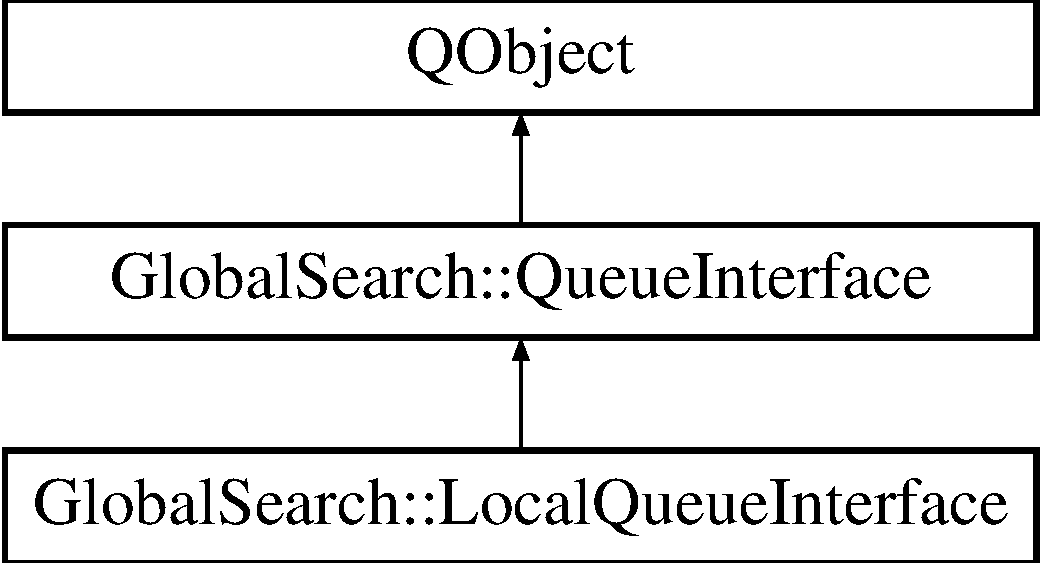
\includegraphics[height=3.000000cm]{classGlobalSearch_1_1QueueInterface}
\end{center}
\end{figure}
\subsection*{Public Types}
\begin{DoxyCompactItemize}
\item 
enum \hyperlink{classGlobalSearch_1_1QueueInterface_a08dcf06d1b99f6333472470490ca9a6d}{Queue\+Status} \{ \\*
\hyperlink{classGlobalSearch_1_1QueueInterface_a08dcf06d1b99f6333472470490ca9a6da4960b69e5e05b425331bba80e5b59e20}{Unknown} = -\/1, 
\hyperlink{classGlobalSearch_1_1QueueInterface_a08dcf06d1b99f6333472470490ca9a6da4be480247388114f3860f7e746df65e9}{Success}, 
\hyperlink{classGlobalSearch_1_1QueueInterface_a08dcf06d1b99f6333472470490ca9a6dabaf3f4a536a56b3a2ac6643de3e4689f}{Error}, 
\hyperlink{classGlobalSearch_1_1QueueInterface_a08dcf06d1b99f6333472470490ca9a6da4c4e184400d3f455f263dc029217fc9a}{Queued}, 
\\*
\hyperlink{classGlobalSearch_1_1QueueInterface_a08dcf06d1b99f6333472470490ca9a6da46d29e0584d720fdb20334913c0a5822}{Running}, 
\hyperlink{classGlobalSearch_1_1QueueInterface_a08dcf06d1b99f6333472470490ca9a6da96ca4ddb429576d197eefe0e6b3a3a98}{Communication\+Error}, 
\hyperlink{classGlobalSearch_1_1QueueInterface_a08dcf06d1b99f6333472470490ca9a6dad54b02ac97bb4a875b105a31489f7aa7}{Started}, 
\hyperlink{classGlobalSearch_1_1QueueInterface_a08dcf06d1b99f6333472470490ca9a6da08ea952b51a67578345517c853e66801}{Pending}
 \}
\end{DoxyCompactItemize}
\subsection*{Public Slots}
\begin{DoxyCompactItemize}
\item 
virtual void \hyperlink{classGlobalSearch_1_1QueueInterface_a6f52e6123a0963a759a18e01804360ac}{read\+Settings} (const Q\+String \&filename=\char`\"{}\char`\"{})
\item 
virtual void \hyperlink{classGlobalSearch_1_1QueueInterface_a2ca92e5132d02e5eda672d2904779a3c}{write\+Settings} (const Q\+String \&filename=\char`\"{}\char`\"{})
\item 
virtual bool \hyperlink{classGlobalSearch_1_1QueueInterface_a4f0c5df9f5945c9c5a64cdf47b7834fa}{write\+Input\+Files} (\hyperlink{classGlobalSearch_1_1Structure}{Structure} $\ast$s) const 
\item 
virtual bool \hyperlink{classGlobalSearch_1_1QueueInterface_a8850904265fa4f397aa37fce9b548829}{write\+Files} (\hyperlink{classGlobalSearch_1_1Structure}{Structure} $\ast$s, const Q\+Hash$<$ Q\+String, Q\+String $>$ \&files) const =0
\item 
virtual bool \hyperlink{classGlobalSearch_1_1QueueInterface_a70a6aa40639e36575a90ffd17c595f55}{start\+Job} (\hyperlink{classGlobalSearch_1_1Structure}{Structure} $\ast$s)=0
\item 
virtual bool \hyperlink{classGlobalSearch_1_1QueueInterface_ab61d5cc09730f42f225571f6865ed383}{stop\+Job} (\hyperlink{classGlobalSearch_1_1Structure}{Structure} $\ast$s)=0
\item 
virtual \hyperlink{classGlobalSearch_1_1QueueInterface_a08dcf06d1b99f6333472470490ca9a6d}{Queue\+Interface\+::\+Queue\+Status} \hyperlink{classGlobalSearch_1_1QueueInterface_a8294808ad1612f2b6fccd932a9d7fd35}{get\+Status} (\hyperlink{classGlobalSearch_1_1Structure}{Structure} $\ast$s) const =0
\item 
virtual bool \hyperlink{classGlobalSearch_1_1QueueInterface_ac3a92214ace255b679951f5a5ef9a11c}{prepare\+For\+Structure\+Update} (\hyperlink{classGlobalSearch_1_1Structure}{Structure} $\ast$s) const =0
\item 
virtual bool \hyperlink{classGlobalSearch_1_1QueueInterface_ab9ea013a587a597749be3efbe035eff8}{check\+If\+File\+Exists} (\hyperlink{classGlobalSearch_1_1Structure}{Structure} $\ast$s, const Q\+String \&filename, bool $\ast$exists)=0
\item 
virtual bool \hyperlink{classGlobalSearch_1_1QueueInterface_ac8af84b05ee61d8c9bb6f1648cc5f221}{fetch\+File} (\hyperlink{classGlobalSearch_1_1Structure}{Structure} $\ast$s, const Q\+String \&filename, Q\+String $\ast$contents) const =0
\item 
virtual bool \hyperlink{classGlobalSearch_1_1QueueInterface_ad3a350e2b2cd0ac746b3c3c22e8606a5}{grep\+File} (\hyperlink{classGlobalSearch_1_1Structure}{Structure} $\ast$s, const Q\+String \&match\+Text, const Q\+String \&filename, Q\+String\+List $\ast$matches=0, int $\ast$exitcode=0, const bool case\+Sensitive=true) const =0
\item 
Q\+String \hyperlink{classGlobalSearch_1_1QueueInterface_a105fbf7ab1565d55cae260269d4be627}{get\+I\+D\+String} () const 
\end{DoxyCompactItemize}
\subsection*{Public Member Functions}
\begin{DoxyCompactItemize}
\item 
\hyperlink{classGlobalSearch_1_1QueueInterface_a77760aeacabb67669a1a32cf3355d472}{Queue\+Interface} (\hyperlink{classGlobalSearch_1_1OptBase}{Opt\+Base} $\ast$parent, const Q\+String \&setting\+File=\char`\"{}\char`\"{})
\item 
virtual \hyperlink{classGlobalSearch_1_1QueueInterface_a3e27228ce5719de17a5fabe8c105d174}{$\sim$\+Queue\+Interface} ()
\item 
virtual bool \hyperlink{classGlobalSearch_1_1QueueInterface_a5da91bc3cd0c30e9a3c7259aada7b5f9}{is\+Ready\+To\+Search} (Q\+String $\ast$err)
\item 
Q\+String\+List \hyperlink{classGlobalSearch_1_1QueueInterface_a1208dba4232727cc026efdf7423f29ad}{get\+Template\+File\+Names} () const 
\item 
bool \hyperlink{group__dialog_gaa78e95fa76777efba3cdfd70d8e3caf9}{has\+Dialog} ()
\item 
virtual Q\+Dialog $\ast$ \hyperlink{group__dialog_ga4457d66b93f0406af1b595659ca25dcf}{dialog} ()
\end{DoxyCompactItemize}
\subsection*{Protected Attributes}
\begin{DoxyCompactItemize}
\item 
\hypertarget{classGlobalSearch_1_1QueueInterface_aadfac830d9d1551ceb3d4c80937c9b9e}{}\hyperlink{classGlobalSearch_1_1OptBase}{Opt\+Base} $\ast$ \hyperlink{classGlobalSearch_1_1QueueInterface_aadfac830d9d1551ceb3d4c80937c9b9e}{m\+\_\+opt}\label{classGlobalSearch_1_1QueueInterface_aadfac830d9d1551ceb3d4c80937c9b9e}

\begin{DoxyCompactList}\small\item\em Cached pointer to the parent \hyperlink{classGlobalSearch_1_1OptBase}{Opt\+Base} class. \end{DoxyCompactList}\item 
\hypertarget{classGlobalSearch_1_1QueueInterface_a695d33f6164f7d83cbe6e0b6d3c5b730}{}Q\+String \hyperlink{classGlobalSearch_1_1QueueInterface_a695d33f6164f7d83cbe6e0b6d3c5b730}{m\+\_\+id\+String}\label{classGlobalSearch_1_1QueueInterface_a695d33f6164f7d83cbe6e0b6d3c5b730}

\begin{DoxyCompactList}\small\item\em String identifying the type of queue interface. \end{DoxyCompactList}\item 
Q\+String\+List \hyperlink{classGlobalSearch_1_1QueueInterface_afbece4079dfba7a2cf11c32153c777a7}{m\+\_\+templates}
\item 
\hypertarget{classGlobalSearch_1_1QueueInterface_a81933da94485f46aec4263172eaf604f}{}bool \hyperlink{classGlobalSearch_1_1QueueInterface_a81933da94485f46aec4263172eaf604f}{m\+\_\+has\+Dialog}\label{classGlobalSearch_1_1QueueInterface_a81933da94485f46aec4263172eaf604f}

\begin{DoxyCompactList}\small\item\em Whether this \hyperlink{classGlobalSearch_1_1QueueInterface}{Queue\+Interface} has a configuration dialog. \end{DoxyCompactList}\item 
\hypertarget{classGlobalSearch_1_1QueueInterface_ae7485212b5aa09c35ec6b1fbfadfeb5d}{}Q\+Dialog $\ast$ \hyperlink{classGlobalSearch_1_1QueueInterface_ae7485212b5aa09c35ec6b1fbfadfeb5d}{m\+\_\+dialog}\label{classGlobalSearch_1_1QueueInterface_ae7485212b5aa09c35ec6b1fbfadfeb5d}

\begin{DoxyCompactList}\small\item\em Pointer to configuration dialog (may be N\+U\+L\+L) \end{DoxyCompactList}\end{DoxyCompactItemize}


\subsection{Detailed Description}
Abstract interface for job submission. 

\begin{DoxyAuthor}{Author}
David C. Lonie
\end{DoxyAuthor}
Do not derive directly from this class. Instead, use Local\+Queue or (more likely) Remote\+Queue.

T\+O\+D\+O detailed description. 

Definition at line 41 of file queueinterface.\+h.



\subsection{Member Enumeration Documentation}
\hypertarget{classGlobalSearch_1_1QueueInterface_a08dcf06d1b99f6333472470490ca9a6d}{}\index{Global\+Search\+::\+Queue\+Interface@{Global\+Search\+::\+Queue\+Interface}!Queue\+Status@{Queue\+Status}}
\index{Queue\+Status@{Queue\+Status}!Global\+Search\+::\+Queue\+Interface@{Global\+Search\+::\+Queue\+Interface}}
\subsubsection[{Queue\+Status}]{\setlength{\rightskip}{0pt plus 5cm}enum {\bf Global\+Search\+::\+Queue\+Interface\+::\+Queue\+Status}}\label{classGlobalSearch_1_1QueueInterface_a08dcf06d1b99f6333472470490ca9a6d}
Possible status for running jobs \begin{DoxySeeAlso}{See also}
\hyperlink{classGlobalSearch_1_1QueueInterface_a8294808ad1612f2b6fccd932a9d7fd35}{get\+Status} 
\end{DoxySeeAlso}
\begin{Desc}
\item[Enumerator]\par
\begin{description}
\index{Unknown@{Unknown}!Global\+Search\+::\+Queue\+Interface@{Global\+Search\+::\+Queue\+Interface}}\index{Global\+Search\+::\+Queue\+Interface@{Global\+Search\+::\+Queue\+Interface}!Unknown@{Unknown}}\item[{\em 
\hypertarget{classGlobalSearch_1_1QueueInterface_a08dcf06d1b99f6333472470490ca9a6da4960b69e5e05b425331bba80e5b59e20}{}Unknown\label{classGlobalSearch_1_1QueueInterface_a08dcf06d1b99f6333472470490ca9a6da4960b69e5e05b425331bba80e5b59e20}
}]Something very bizarre has happened. \index{Success@{Success}!Global\+Search\+::\+Queue\+Interface@{Global\+Search\+::\+Queue\+Interface}}\index{Global\+Search\+::\+Queue\+Interface@{Global\+Search\+::\+Queue\+Interface}!Success@{Success}}\item[{\em 
\hypertarget{classGlobalSearch_1_1QueueInterface_a08dcf06d1b99f6333472470490ca9a6da4be480247388114f3860f7e746df65e9}{}Success\label{classGlobalSearch_1_1QueueInterface_a08dcf06d1b99f6333472470490ca9a6da4be480247388114f3860f7e746df65e9}
}]Job has completed successfully. \index{Error@{Error}!Global\+Search\+::\+Queue\+Interface@{Global\+Search\+::\+Queue\+Interface}}\index{Global\+Search\+::\+Queue\+Interface@{Global\+Search\+::\+Queue\+Interface}!Error@{Error}}\item[{\em 
\hypertarget{classGlobalSearch_1_1QueueInterface_a08dcf06d1b99f6333472470490ca9a6dabaf3f4a536a56b3a2ac6643de3e4689f}{}Error\label{classGlobalSearch_1_1QueueInterface_a08dcf06d1b99f6333472470490ca9a6dabaf3f4a536a56b3a2ac6643de3e4689f}
}]Job finished, but the optimization was unsuccessful. \index{Queued@{Queued}!Global\+Search\+::\+Queue\+Interface@{Global\+Search\+::\+Queue\+Interface}}\index{Global\+Search\+::\+Queue\+Interface@{Global\+Search\+::\+Queue\+Interface}!Queued@{Queued}}\item[{\em 
\hypertarget{classGlobalSearch_1_1QueueInterface_a08dcf06d1b99f6333472470490ca9a6da4c4e184400d3f455f263dc029217fc9a}{}Queued\label{classGlobalSearch_1_1QueueInterface_a08dcf06d1b99f6333472470490ca9a6da4c4e184400d3f455f263dc029217fc9a}
}]Job is queued. \index{Running@{Running}!Global\+Search\+::\+Queue\+Interface@{Global\+Search\+::\+Queue\+Interface}}\index{Global\+Search\+::\+Queue\+Interface@{Global\+Search\+::\+Queue\+Interface}!Running@{Running}}\item[{\em 
\hypertarget{classGlobalSearch_1_1QueueInterface_a08dcf06d1b99f6333472470490ca9a6da46d29e0584d720fdb20334913c0a5822}{}Running\label{classGlobalSearch_1_1QueueInterface_a08dcf06d1b99f6333472470490ca9a6da46d29e0584d720fdb20334913c0a5822}
}]Job is current running. \index{Communication\+Error@{Communication\+Error}!Global\+Search\+::\+Queue\+Interface@{Global\+Search\+::\+Queue\+Interface}}\index{Global\+Search\+::\+Queue\+Interface@{Global\+Search\+::\+Queue\+Interface}!Communication\+Error@{Communication\+Error}}\item[{\em 
\hypertarget{classGlobalSearch_1_1QueueInterface_a08dcf06d1b99f6333472470490ca9a6da96ca4ddb429576d197eefe0e6b3a3a98}{}Communication\+Error\label{classGlobalSearch_1_1QueueInterface_a08dcf06d1b99f6333472470490ca9a6da96ca4ddb429576d197eefe0e6b3a3a98}
}]Communication with a remote server has failed. \index{Started@{Started}!Global\+Search\+::\+Queue\+Interface@{Global\+Search\+::\+Queue\+Interface}}\index{Global\+Search\+::\+Queue\+Interface@{Global\+Search\+::\+Queue\+Interface}!Started@{Started}}\item[{\em 
\hypertarget{classGlobalSearch_1_1QueueInterface_a08dcf06d1b99f6333472470490ca9a6dad54b02ac97bb4a875b105a31489f7aa7}{}Started\label{classGlobalSearch_1_1QueueInterface_a08dcf06d1b99f6333472470490ca9a6dad54b02ac97bb4a875b105a31489f7aa7}
}]Job has appeared in queue, but the \hyperlink{classGlobalSearch_1_1Structure}{Structure} still returns \hyperlink{classGlobalSearch_1_1Structure_a3f1e44cb4f603fe1b3fbc8e813535917a5a0e4ad5830e2c3a9b045da79098b6c7}{Structure\+::\+Submitted} instead of \hyperlink{classGlobalSearch_1_1Structure_a3f1e44cb4f603fe1b3fbc8e813535917a4f451a4c3de6ed294e1c7d06e5b1d24c}{Structure\+::\+In\+Process}. This will be corrected in the next iteration of \hyperlink{classGlobalSearch_1_1QueueManager_a2a85ad6729d9e0eb13782699b6cd5ccd}{Queue\+Manager\+::check\+Running()}. \index{Pending@{Pending}!Global\+Search\+::\+Queue\+Interface@{Global\+Search\+::\+Queue\+Interface}}\index{Global\+Search\+::\+Queue\+Interface@{Global\+Search\+::\+Queue\+Interface}!Pending@{Pending}}\item[{\em 
\hypertarget{classGlobalSearch_1_1QueueInterface_a08dcf06d1b99f6333472470490ca9a6da08ea952b51a67578345517c853e66801}{}Pending\label{classGlobalSearch_1_1QueueInterface_a08dcf06d1b99f6333472470490ca9a6da08ea952b51a67578345517c853e66801}
}]Job has been submitted, but has not appeared in queue. \end{description}
\end{Desc}


Definition at line 65 of file queueinterface.\+h.



\subsection{Constructor \& Destructor Documentation}
\hypertarget{classGlobalSearch_1_1QueueInterface_a77760aeacabb67669a1a32cf3355d472}{}\index{Global\+Search\+::\+Queue\+Interface@{Global\+Search\+::\+Queue\+Interface}!Queue\+Interface@{Queue\+Interface}}
\index{Queue\+Interface@{Queue\+Interface}!Global\+Search\+::\+Queue\+Interface@{Global\+Search\+::\+Queue\+Interface}}
\subsubsection[{Queue\+Interface}]{\setlength{\rightskip}{0pt plus 5cm}Global\+Search\+::\+Queue\+Interface\+::\+Queue\+Interface (
\begin{DoxyParamCaption}
\item[{{\bf Opt\+Base} $\ast$}]{parent, }
\item[{const Q\+String \&}]{setting\+File = {\ttfamily \char`\"{}\char`\"{}}}
\end{DoxyParamCaption}
)\hspace{0.3cm}{\ttfamily [inline]}, {\ttfamily [explicit]}}\label{classGlobalSearch_1_1QueueInterface_a77760aeacabb67669a1a32cf3355d472}
Constructor


\begin{DoxyParams}{Parameters}
{\em parent} & \hyperlink{classGlobalSearch_1_1OptBase}{Opt\+Base} parent \\
\hline
{\em setting\+File} & Filename from which to initialize settings. \\
\hline
\end{DoxyParams}


Definition at line 52 of file queueinterface.\+h.

\hypertarget{classGlobalSearch_1_1QueueInterface_a3e27228ce5719de17a5fabe8c105d174}{}\index{Global\+Search\+::\+Queue\+Interface@{Global\+Search\+::\+Queue\+Interface}!````~Queue\+Interface@{$\sim$\+Queue\+Interface}}
\index{````~Queue\+Interface@{$\sim$\+Queue\+Interface}!Global\+Search\+::\+Queue\+Interface@{Global\+Search\+::\+Queue\+Interface}}
\subsubsection[{$\sim$\+Queue\+Interface}]{\setlength{\rightskip}{0pt plus 5cm}virtual Global\+Search\+::\+Queue\+Interface\+::$\sim$\+Queue\+Interface (
\begin{DoxyParamCaption}
{}
\end{DoxyParamCaption}
)\hspace{0.3cm}{\ttfamily [inline]}, {\ttfamily [virtual]}}\label{classGlobalSearch_1_1QueueInterface_a3e27228ce5719de17a5fabe8c105d174}
Destructor 

Definition at line 59 of file queueinterface.\+h.



\subsection{Member Function Documentation}
\hypertarget{classGlobalSearch_1_1QueueInterface_ab9ea013a587a597749be3efbe035eff8}{}\index{Global\+Search\+::\+Queue\+Interface@{Global\+Search\+::\+Queue\+Interface}!check\+If\+File\+Exists@{check\+If\+File\+Exists}}
\index{check\+If\+File\+Exists@{check\+If\+File\+Exists}!Global\+Search\+::\+Queue\+Interface@{Global\+Search\+::\+Queue\+Interface}}
\subsubsection[{check\+If\+File\+Exists}]{\setlength{\rightskip}{0pt plus 5cm}virtual bool Global\+Search\+::\+Queue\+Interface\+::check\+If\+File\+Exists (
\begin{DoxyParamCaption}
\item[{{\bf Structure} $\ast$}]{s, }
\item[{const Q\+String \&}]{filename, }
\item[{bool $\ast$}]{exists}
\end{DoxyParamCaption}
)\hspace{0.3cm}{\ttfamily [pure virtual]}, {\ttfamily [slot]}}\label{classGlobalSearch_1_1QueueInterface_ab9ea013a587a597749be3efbe035eff8}
Check if the file {\itshape filename} exists in the working directory of \hyperlink{classGlobalSearch_1_1Structure}{Structure} {\itshape s} and store the result in {\itshape exists}.

\begin{DoxyNote}{Note}
This function uses the argument {\itshape exists} to report whether or not the file exists. The return value indicates whether the file check was performed without errors (e.\+g. network errors).
\end{DoxyNote}
\begin{DoxyReturn}{Returns}
True if the test encountered no errors, false otherwise. 
\end{DoxyReturn}


Referenced by Global\+Search\+::\+Optimizer\+::check\+If\+Output\+File\+Exists().

\hypertarget{classGlobalSearch_1_1QueueInterface_ac8af84b05ee61d8c9bb6f1648cc5f221}{}\index{Global\+Search\+::\+Queue\+Interface@{Global\+Search\+::\+Queue\+Interface}!fetch\+File@{fetch\+File}}
\index{fetch\+File@{fetch\+File}!Global\+Search\+::\+Queue\+Interface@{Global\+Search\+::\+Queue\+Interface}}
\subsubsection[{fetch\+File}]{\setlength{\rightskip}{0pt plus 5cm}virtual bool Global\+Search\+::\+Queue\+Interface\+::fetch\+File (
\begin{DoxyParamCaption}
\item[{{\bf Structure} $\ast$}]{s, }
\item[{const Q\+String \&}]{filename, }
\item[{Q\+String $\ast$}]{contents}
\end{DoxyParamCaption}
) const\hspace{0.3cm}{\ttfamily [pure virtual]}, {\ttfamily [slot]}}\label{classGlobalSearch_1_1QueueInterface_ac8af84b05ee61d8c9bb6f1648cc5f221}
Retrieve the contents of the file {\itshape filename} for \hyperlink{classGlobalSearch_1_1Structure}{Structure} {\itshape s} as a Q\+String {\itshape contents}.

\begin{DoxyReturn}{Returns}
True on success, false otherwise. 
\end{DoxyReturn}
\hypertarget{classGlobalSearch_1_1QueueInterface_a105fbf7ab1565d55cae260269d4be627}{}\index{Global\+Search\+::\+Queue\+Interface@{Global\+Search\+::\+Queue\+Interface}!get\+I\+D\+String@{get\+I\+D\+String}}
\index{get\+I\+D\+String@{get\+I\+D\+String}!Global\+Search\+::\+Queue\+Interface@{Global\+Search\+::\+Queue\+Interface}}
\subsubsection[{get\+I\+D\+String}]{\setlength{\rightskip}{0pt plus 5cm}Q\+String Global\+Search\+::\+Queue\+Interface\+::get\+I\+D\+String (
\begin{DoxyParamCaption}
{}
\end{DoxyParamCaption}
) const\hspace{0.3cm}{\ttfamily [inline]}, {\ttfamily [slot]}}\label{classGlobalSearch_1_1QueueInterface_a105fbf7ab1565d55cae260269d4be627}
\begin{DoxyReturn}{Returns}
The name of the queue interface (e.\+g. \char`\"{}\+Local\char`\"{}, \char`\"{}\+P\+B\+S\char`\"{}, etc) 
\end{DoxyReturn}


Definition at line 249 of file queueinterface.\+h.



References m\+\_\+id\+String.



Referenced by Global\+Search\+::\+Optimizer\+::read\+Templates\+From\+Settings(), and Global\+Search\+::\+Optimizer\+::write\+Templates\+To\+Settings().

\hypertarget{classGlobalSearch_1_1QueueInterface_a8294808ad1612f2b6fccd932a9d7fd35}{}\index{Global\+Search\+::\+Queue\+Interface@{Global\+Search\+::\+Queue\+Interface}!get\+Status@{get\+Status}}
\index{get\+Status@{get\+Status}!Global\+Search\+::\+Queue\+Interface@{Global\+Search\+::\+Queue\+Interface}}
\subsubsection[{get\+Status}]{\setlength{\rightskip}{0pt plus 5cm}virtual {\bf Queue\+Interface\+::\+Queue\+Status} Global\+Search\+::\+Queue\+Interface\+::get\+Status (
\begin{DoxyParamCaption}
\item[{{\bf Structure} $\ast$}]{s}
\end{DoxyParamCaption}
) const\hspace{0.3cm}{\ttfamily [pure virtual]}, {\ttfamily [slot]}}\label{classGlobalSearch_1_1QueueInterface_a8294808ad1612f2b6fccd932a9d7fd35}
\begin{DoxyReturn}{Returns}
The queue status of \hyperlink{classGlobalSearch_1_1Structure}{Structure} {\itshape s}. 
\end{DoxyReturn}
\hypertarget{classGlobalSearch_1_1QueueInterface_a1208dba4232727cc026efdf7423f29ad}{}\index{Global\+Search\+::\+Queue\+Interface@{Global\+Search\+::\+Queue\+Interface}!get\+Template\+File\+Names@{get\+Template\+File\+Names}}
\index{get\+Template\+File\+Names@{get\+Template\+File\+Names}!Global\+Search\+::\+Queue\+Interface@{Global\+Search\+::\+Queue\+Interface}}
\subsubsection[{get\+Template\+File\+Names}]{\setlength{\rightskip}{0pt plus 5cm}Q\+String\+List Global\+Search\+::\+Queue\+Interface\+::get\+Template\+File\+Names (
\begin{DoxyParamCaption}
{}
\end{DoxyParamCaption}
) const\hspace{0.3cm}{\ttfamily [inline]}}\label{classGlobalSearch_1_1QueueInterface_a1208dba4232727cc026efdf7423f29ad}
\begin{DoxyReturn}{Returns}
The names of all template files associated with this interface. 
\end{DoxyReturn}


Definition at line 255 of file queueinterface.\+h.



References m\+\_\+templates.



Referenced by Global\+Search\+::\+Abstract\+Edit\+Tab\+::get\+Template\+Names(), and Global\+Search\+::\+Optimizer\+::update\+Queue\+Interface().

\hypertarget{classGlobalSearch_1_1QueueInterface_ad3a350e2b2cd0ac746b3c3c22e8606a5}{}\index{Global\+Search\+::\+Queue\+Interface@{Global\+Search\+::\+Queue\+Interface}!grep\+File@{grep\+File}}
\index{grep\+File@{grep\+File}!Global\+Search\+::\+Queue\+Interface@{Global\+Search\+::\+Queue\+Interface}}
\subsubsection[{grep\+File}]{\setlength{\rightskip}{0pt plus 5cm}virtual bool Global\+Search\+::\+Queue\+Interface\+::grep\+File (
\begin{DoxyParamCaption}
\item[{{\bf Structure} $\ast$}]{s, }
\item[{const Q\+String \&}]{match\+Text, }
\item[{const Q\+String \&}]{filename, }
\item[{Q\+String\+List $\ast$}]{matches = {\ttfamily 0}, }
\item[{int $\ast$}]{exitcode = {\ttfamily 0}, }
\item[{const bool}]{case\+Sensitive = {\ttfamily true}}
\end{DoxyParamCaption}
) const\hspace{0.3cm}{\ttfamily [pure virtual]}, {\ttfamily [slot]}}\label{classGlobalSearch_1_1QueueInterface_ad3a350e2b2cd0ac746b3c3c22e8606a5}
Grep through the file {\itshape filename} in \hyperlink{classGlobalSearch_1_1Structure}{Structure} {\itshape s\textquotesingle{}s} working directory, looking for {\itshape match\+Text}. The list of matches is returned in the Q\+String\+List {\itshape matches} and the exit status is returned as {\itshape exitcode}.

Possible exitcodes\+:
\begin{DoxyItemize}
\item 0\+: Matches were found, execution successful
\item 1\+: No matches found, execution successful
\item 2\+: Execution unsuccessful
\end{DoxyItemize}


\begin{DoxyParams}{Parameters}
{\em s} & \hyperlink{classGlobalSearch_1_1Structure}{Structure} of interest \\
\hline
{\em match\+Text} & Text to match \\
\hline
{\em filename} & Name of file to grep \\
\hline
{\em matches} & List of matches (return) \\
\hline
{\em exitcode} & Exit code of grep (see details) (return) \\
\hline
{\em case\+Sensitive} & If true, match case. Otherwise, perform case-\/insensitive search (e.\+g. grep -\/i) Default is true.\\
\hline
\end{DoxyParams}
\begin{DoxyReturn}{Returns}
True on success, false otherwise.
\end{DoxyReturn}
\begin{DoxyNote}{Note}
There are two types of failure possible here\+: Either the {\itshape exitcode} can be 2 or the function can return false. If the {\itshape exitcode} is 2, then grep failed to execute. If false, then there was a failure in the interface code, likely a communication error with a remote server.

On local queue interface, grep is not actually used and the exit code behavior is emulated. 
\end{DoxyNote}


Referenced by Global\+Search\+::\+Optimizer\+::check\+For\+Successful\+Output().

\hypertarget{classGlobalSearch_1_1QueueInterface_a5da91bc3cd0c30e9a3c7259aada7b5f9}{}\index{Global\+Search\+::\+Queue\+Interface@{Global\+Search\+::\+Queue\+Interface}!is\+Ready\+To\+Search@{is\+Ready\+To\+Search}}
\index{is\+Ready\+To\+Search@{is\+Ready\+To\+Search}!Global\+Search\+::\+Queue\+Interface@{Global\+Search\+::\+Queue\+Interface}}
\subsubsection[{is\+Ready\+To\+Search}]{\setlength{\rightskip}{0pt plus 5cm}virtual bool Global\+Search\+::\+Queue\+Interface\+::is\+Ready\+To\+Search (
\begin{DoxyParamCaption}
\item[{Q\+String $\ast$}]{err}
\end{DoxyParamCaption}
)\hspace{0.3cm}{\ttfamily [inline]}, {\ttfamily [virtual]}}\label{classGlobalSearch_1_1QueueInterface_a5da91bc3cd0c30e9a3c7259aada7b5f9}
Check that all mandatory internal variables are set. Check this before starting a search.


\begin{DoxyParams}{Parameters}
{\em err} & String to be overwritten with an error message\\
\hline
\end{DoxyParams}
\begin{DoxyReturn}{Returns}
true if all variables are initialized, false otherwise. If false, {\itshape err} will be overwritten with a user-\/friendly error message. 
\end{DoxyReturn}


Reimplemented in \hyperlink{classGlobalSearch_1_1LocalQueueInterface_ab414f1b5b47610e45fece054512566ed}{Global\+Search\+::\+Local\+Queue\+Interface}.



Definition at line 97 of file queueinterface.\+h.

\hypertarget{classGlobalSearch_1_1QueueInterface_ac3a92214ace255b679951f5a5ef9a11c}{}\index{Global\+Search\+::\+Queue\+Interface@{Global\+Search\+::\+Queue\+Interface}!prepare\+For\+Structure\+Update@{prepare\+For\+Structure\+Update}}
\index{prepare\+For\+Structure\+Update@{prepare\+For\+Structure\+Update}!Global\+Search\+::\+Queue\+Interface@{Global\+Search\+::\+Queue\+Interface}}
\subsubsection[{prepare\+For\+Structure\+Update}]{\setlength{\rightskip}{0pt plus 5cm}virtual bool Global\+Search\+::\+Queue\+Interface\+::prepare\+For\+Structure\+Update (
\begin{DoxyParamCaption}
\item[{{\bf Structure} $\ast$}]{s}
\end{DoxyParamCaption}
) const\hspace{0.3cm}{\ttfamily [pure virtual]}, {\ttfamily [slot]}}\label{classGlobalSearch_1_1QueueInterface_ac3a92214ace255b679951f5a5ef9a11c}
Perform any work needed before calling \hyperlink{classGlobalSearch_1_1Optimizer_a7e57844e4e6d713c87e6cf29ea03c5e2}{Optimizer\+::update}. This function mainly exists for Remote\+Queue classes to copy files back from the server, but may be used for other purposes. It is guaranteed to be called by \hyperlink{classGlobalSearch_1_1Optimizer}{Optimizer} before updating.


\begin{DoxyParams}{Parameters}
{\em s} & The structure that is to be updated.\\
\hline
\end{DoxyParams}
\begin{DoxyReturn}{Returns}
True on success, false otherwise. 
\end{DoxyReturn}


Referenced by Global\+Search\+::\+Optimizer\+::update().

\hypertarget{classGlobalSearch_1_1QueueInterface_a6f52e6123a0963a759a18e01804360ac}{}\index{Global\+Search\+::\+Queue\+Interface@{Global\+Search\+::\+Queue\+Interface}!read\+Settings@{read\+Settings}}
\index{read\+Settings@{read\+Settings}!Global\+Search\+::\+Queue\+Interface@{Global\+Search\+::\+Queue\+Interface}}
\subsubsection[{read\+Settings}]{\setlength{\rightskip}{0pt plus 5cm}virtual void Global\+Search\+::\+Queue\+Interface\+::read\+Settings (
\begin{DoxyParamCaption}
\item[{const Q\+String \&}]{filename = {\ttfamily \char`\"{}\char`\"{}}}
\end{DoxyParamCaption}
)\hspace{0.3cm}{\ttfamily [inline]}, {\ttfamily [virtual]}, {\ttfamily [slot]}}\label{classGlobalSearch_1_1QueueInterface_a6f52e6123a0963a759a18e01804360ac}
Read optimizer data from file (.scheme or .state). If called without an argument, this function does nothing, i.\+e. it will not read optimizer data from the system config file.


\begin{DoxyParams}{Parameters}
{\em filename} & Scheme or state file to load data from. \\
\hline
\end{DoxyParams}
\begin{DoxySeeAlso}{See also}
\hyperlink{classGlobalSearch_1_1QueueInterface_a2ca92e5132d02e5eda672d2904779a3c}{write\+Settings} 
\end{DoxySeeAlso}


Definition at line 109 of file queueinterface.\+h.

\hypertarget{classGlobalSearch_1_1QueueInterface_a70a6aa40639e36575a90ffd17c595f55}{}\index{Global\+Search\+::\+Queue\+Interface@{Global\+Search\+::\+Queue\+Interface}!start\+Job@{start\+Job}}
\index{start\+Job@{start\+Job}!Global\+Search\+::\+Queue\+Interface@{Global\+Search\+::\+Queue\+Interface}}
\subsubsection[{start\+Job}]{\setlength{\rightskip}{0pt plus 5cm}virtual bool Global\+Search\+::\+Queue\+Interface\+::start\+Job (
\begin{DoxyParamCaption}
\item[{{\bf Structure} $\ast$}]{s}
\end{DoxyParamCaption}
)\hspace{0.3cm}{\ttfamily [pure virtual]}, {\ttfamily [slot]}}\label{classGlobalSearch_1_1QueueInterface_a70a6aa40639e36575a90ffd17c595f55}
Start a job for \hyperlink{classGlobalSearch_1_1Structure}{Structure} {\itshape s}.

\begin{DoxyNote}{Note}
Ensure that write\+Files is called before attempting to start the job.
\end{DoxyNote}
\begin{DoxyReturn}{Returns}
True on success, false otherwise. 
\end{DoxyReturn}


Referenced by Global\+Search\+::\+Queue\+Manager\+::start\+Job().

\hypertarget{classGlobalSearch_1_1QueueInterface_ab61d5cc09730f42f225571f6865ed383}{}\index{Global\+Search\+::\+Queue\+Interface@{Global\+Search\+::\+Queue\+Interface}!stop\+Job@{stop\+Job}}
\index{stop\+Job@{stop\+Job}!Global\+Search\+::\+Queue\+Interface@{Global\+Search\+::\+Queue\+Interface}}
\subsubsection[{stop\+Job}]{\setlength{\rightskip}{0pt plus 5cm}virtual bool Global\+Search\+::\+Queue\+Interface\+::stop\+Job (
\begin{DoxyParamCaption}
\item[{{\bf Structure} $\ast$}]{s}
\end{DoxyParamCaption}
)\hspace{0.3cm}{\ttfamily [pure virtual]}, {\ttfamily [slot]}}\label{classGlobalSearch_1_1QueueInterface_ab61d5cc09730f42f225571f6865ed383}
Stop any currently running jobs for \hyperlink{classGlobalSearch_1_1Structure}{Structure} {\itshape s}.

\begin{DoxyReturn}{Returns}
True on success, false otherwise. 
\end{DoxyReturn}


Referenced by Global\+Search\+::\+Optimizer\+::get\+Interpreted\+Templates(), and Global\+Search\+::\+Queue\+Manager\+::stop\+Job().

\hypertarget{classGlobalSearch_1_1QueueInterface_a8850904265fa4f397aa37fce9b548829}{}\index{Global\+Search\+::\+Queue\+Interface@{Global\+Search\+::\+Queue\+Interface}!write\+Files@{write\+Files}}
\index{write\+Files@{write\+Files}!Global\+Search\+::\+Queue\+Interface@{Global\+Search\+::\+Queue\+Interface}}
\subsubsection[{write\+Files}]{\setlength{\rightskip}{0pt plus 5cm}virtual bool Global\+Search\+::\+Queue\+Interface\+::write\+Files (
\begin{DoxyParamCaption}
\item[{{\bf Structure} $\ast$}]{s, }
\item[{const Q\+Hash$<$ Q\+String, Q\+String $>$ \&}]{files}
\end{DoxyParamCaption}
) const\hspace{0.3cm}{\ttfamily [pure virtual]}, {\ttfamily [slot]}}\label{classGlobalSearch_1_1QueueInterface_a8850904265fa4f397aa37fce9b548829}
Write the provided files in the hash {\itshape files} to the local working directory for \hyperlink{classGlobalSearch_1_1Structure}{Structure} {\itshape s} and (if appropriate) copy them to a remote server.


\begin{DoxyParams}{Parameters}
{\em s} & \hyperlink{classGlobalSearch_1_1Structure}{Structure} of interest \\
\hline
{\em files} & Key\+: filename, Value\+: text.\\
\hline
\end{DoxyParams}
\begin{DoxyNote}{Note}
The filenames in {\itshape files} must not be absolute, but relative to the structure\textquotesingle{}s working directory.
\end{DoxyNote}
\begin{DoxyReturn}{Returns}
True on success, false otherwise. 
\end{DoxyReturn}


Referenced by write\+Input\+Files().

\hypertarget{classGlobalSearch_1_1QueueInterface_a4f0c5df9f5945c9c5a64cdf47b7834fa}{}\index{Global\+Search\+::\+Queue\+Interface@{Global\+Search\+::\+Queue\+Interface}!write\+Input\+Files@{write\+Input\+Files}}
\index{write\+Input\+Files@{write\+Input\+Files}!Global\+Search\+::\+Queue\+Interface@{Global\+Search\+::\+Queue\+Interface}}
\subsubsection[{write\+Input\+Files}]{\setlength{\rightskip}{0pt plus 5cm}bool Global\+Search\+::\+Queue\+Interface\+::write\+Input\+Files (
\begin{DoxyParamCaption}
\item[{{\bf Structure} $\ast$}]{s}
\end{DoxyParamCaption}
) const\hspace{0.3cm}{\ttfamily [virtual]}, {\ttfamily [slot]}}\label{classGlobalSearch_1_1QueueInterface_a4f0c5df9f5945c9c5a64cdf47b7834fa}
Write the input files for \hyperlink{classGlobalSearch_1_1Structure}{Structure} {\itshape s} to the appropriate location.

This function will also construct and write any queue-\/specific files (e.\+g. job.\+pbs for P\+B\+S queues) and copy them to the remote host if using a remote queue.

\begin{DoxyReturn}{Returns}
True on success, false otherwise. 
\end{DoxyReturn}


Definition at line 28 of file queueinterface.\+cpp.



References Global\+Search\+::\+Optimizer\+::get\+Interpreted\+Templates(), m\+\_\+opt, Global\+Search\+::\+Opt\+Base\+::optimizer(), and write\+Files().

\hypertarget{classGlobalSearch_1_1QueueInterface_a2ca92e5132d02e5eda672d2904779a3c}{}\index{Global\+Search\+::\+Queue\+Interface@{Global\+Search\+::\+Queue\+Interface}!write\+Settings@{write\+Settings}}
\index{write\+Settings@{write\+Settings}!Global\+Search\+::\+Queue\+Interface@{Global\+Search\+::\+Queue\+Interface}}
\subsubsection[{write\+Settings}]{\setlength{\rightskip}{0pt plus 5cm}virtual void Global\+Search\+::\+Queue\+Interface\+::write\+Settings (
\begin{DoxyParamCaption}
\item[{const Q\+String \&}]{filename = {\ttfamily \char`\"{}\char`\"{}}}
\end{DoxyParamCaption}
)\hspace{0.3cm}{\ttfamily [inline]}, {\ttfamily [virtual]}, {\ttfamily [slot]}}\label{classGlobalSearch_1_1QueueInterface_a2ca92e5132d02e5eda672d2904779a3c}
Write optimizer data to file (.scheme or .state). If called without an argument, this function does nothing, i.\+e. it will not write optimizer data to the system config file.


\begin{DoxyParams}{Parameters}
{\em filename} & Scheme or state file to write data to. \\
\hline
\end{DoxyParams}
\begin{DoxySeeAlso}{See also}
\hyperlink{classGlobalSearch_1_1QueueInterface_a6f52e6123a0963a759a18e01804360ac}{read\+Settings} 
\end{DoxySeeAlso}


Definition at line 119 of file queueinterface.\+h.



Referenced by Global\+Search\+::\+Optimizer\+::write\+Settings().



\subsection{Member Data Documentation}
\hypertarget{classGlobalSearch_1_1QueueInterface_afbece4079dfba7a2cf11c32153c777a7}{}\index{Global\+Search\+::\+Queue\+Interface@{Global\+Search\+::\+Queue\+Interface}!m\+\_\+templates@{m\+\_\+templates}}
\index{m\+\_\+templates@{m\+\_\+templates}!Global\+Search\+::\+Queue\+Interface@{Global\+Search\+::\+Queue\+Interface}}
\subsubsection[{m\+\_\+templates}]{\setlength{\rightskip}{0pt plus 5cm}Q\+String\+List Global\+Search\+::\+Queue\+Interface\+::m\+\_\+templates\hspace{0.3cm}{\ttfamily [protected]}}\label{classGlobalSearch_1_1QueueInterface_afbece4079dfba7a2cf11c32153c777a7}
Q\+String\+List containing list of all template filenames \begin{DoxyNote}{Note}
templates are actually handled in \hyperlink{classGlobalSearch_1_1Optimizer}{Optimizer} 
\end{DoxyNote}


Definition at line 283 of file queueinterface.\+h.



Referenced by get\+Template\+File\+Names().



The documentation for this class was generated from the following files\+:\begin{DoxyCompactItemize}
\item 
src/globalsearch/queueinterface.\+h\item 
src/globalsearch/queueinterface.\+cpp\end{DoxyCompactItemize}

\hypertarget{classGlobalSearch_1_1QueueManager}{}\section{Global\+Search\+:\+:Queue\+Manager Class Reference}
\label{classGlobalSearch_1_1QueueManager}\index{Global\+Search\+::\+Queue\+Manager@{Global\+Search\+::\+Queue\+Manager}}


The \hyperlink{classGlobalSearch_1_1QueueManager}{Queue\+Manager} monitors the running jobs and updates \hyperlink{classGlobalSearch_1_1Structure}{Structure} status.  




{\ttfamily \#include $<$globalsearch/queuemanager.\+h$>$}

Inheritance diagram for Global\+Search\+:\+:Queue\+Manager\+:\begin{figure}[H]
\begin{center}
\leavevmode
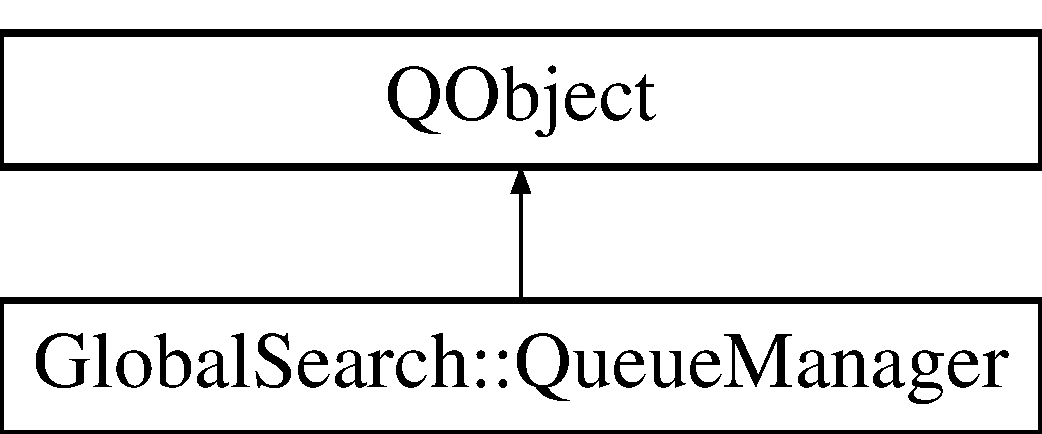
\includegraphics[height=2.000000cm]{classGlobalSearch_1_1QueueManager}
\end{center}
\end{figure}
\subsection*{Public Slots}
\begin{DoxyCompactItemize}
\item 
void \hyperlink{classGlobalSearch_1_1QueueManager_a36c7fd5b33bd74babfd68ee746e5017c}{reset} ()
\item 
void \hyperlink{classGlobalSearch_1_1QueueManager_aa79f26f791ec8315f2ae36d820bfa0ac}{kill\+Structure} (\hyperlink{classGlobalSearch_1_1Structure}{Structure} $\ast$s)
\item 
void \hyperlink{classGlobalSearch_1_1QueueManager_aa010ca43a5ec0c5ce653c4ab5bfebb27}{append\+To\+Job\+Start\+Tracker} (\hyperlink{classGlobalSearch_1_1Structure}{Structure} $\ast$s)
\item 
void \hyperlink{classGlobalSearch_1_1QueueManager_ab04255999ca9a52f471b37141e9e3f6e}{add\+Manual\+Structure\+Request} (int requests=1)
\item 
Q\+List$<$ \hyperlink{classGlobalSearch_1_1Structure}{Structure} $\ast$ $>$ \hyperlink{classGlobalSearch_1_1QueueManager_abb5985273cbb0126bf065acb76c2be51}{get\+All\+Running\+Structures} ()
\item 
Q\+List$<$ \hyperlink{classGlobalSearch_1_1Structure}{Structure} $\ast$ $>$ \hyperlink{classGlobalSearch_1_1QueueManager_a05ab94e45df60fb8c9078fbf81a2d80c}{get\+All\+Optimized\+Structures} ()
\item 
Q\+List$<$ \hyperlink{classGlobalSearch_1_1Structure}{Structure} $\ast$ $>$ \hyperlink{classGlobalSearch_1_1QueueManager_a14ab987c7a7939e27ba84010e9943bdd}{get\+All\+Duplicate\+Structures} ()
\item 
Q\+List$<$ \hyperlink{classGlobalSearch_1_1Structure}{Structure} $\ast$ $>$ \hyperlink{classGlobalSearch_1_1QueueManager_ad77db239019da90a79040b680f2398dc}{get\+All\+Structures} ()
\item 
Q\+List$<$ \hyperlink{classGlobalSearch_1_1Structure}{Structure} $\ast$ $>$ \hyperlink{classGlobalSearch_1_1QueueManager_a11aa65d1cc9c13424a8eac1c08fe9c0b}{lock\+For\+Naming} ()
\item 
void \hyperlink{classGlobalSearch_1_1QueueManager_a5f8012e4b5d002c444bfc486084feec1}{unlock\+For\+Naming} (\hyperlink{classGlobalSearch_1_1Structure}{Structure} $\ast$s=0)
\end{DoxyCompactItemize}
\subsection*{Signals}
\begin{DoxyCompactItemize}
\item 
void \hyperlink{classGlobalSearch_1_1QueueManager_a1453d56d967bc6ddaaca951c5a7d8c8f}{moved\+To\+Q\+M\+Thread} ()
\item 
void \hyperlink{classGlobalSearch_1_1QueueManager_a4309c24054c4752705f1d66d08358c9f}{structure\+Started} (\hyperlink{classGlobalSearch_1_1Structure}{Global\+Search\+::\+Structure} $\ast$s)
\item 
void \hyperlink{classGlobalSearch_1_1QueueManager_a97ce1e692cd752d62ebea8b2c56e1cd2}{structure\+Submitted} (\hyperlink{classGlobalSearch_1_1Structure}{Global\+Search\+::\+Structure} $\ast$s)
\item 
void \hyperlink{classGlobalSearch_1_1QueueManager_ad6e65416801d0cad4086fafb03990273}{structure\+Killed} (\hyperlink{classGlobalSearch_1_1Structure}{Global\+Search\+::\+Structure} $\ast$s)
\item 
void \hyperlink{classGlobalSearch_1_1QueueManager_aaf98cf54afb9751e185a5450c32f4595}{structure\+Updated} (\hyperlink{classGlobalSearch_1_1Structure}{Global\+Search\+::\+Structure} $\ast$s)
\item 
void \hyperlink{classGlobalSearch_1_1QueueManager_a9ce76b6d4be1aaa3e1f04724f9baa03a}{structure\+Finished} (\hyperlink{classGlobalSearch_1_1Structure}{Global\+Search\+::\+Structure} $\ast$s)
\item 
void \hyperlink{classGlobalSearch_1_1QueueManager_a4b50dbd51e53b1d0d5cb93e9d7380c1c}{need\+New\+Structure} ()
\item 
void \hyperlink{classGlobalSearch_1_1QueueManager_af37eb7a9e54e347a81dc3a1e373c8d54}{new\+Status\+Overview} (int optimized, int running, int failing)
\end{DoxyCompactItemize}
\subsection*{Public Member Functions}
\begin{DoxyCompactItemize}
\item 
\hyperlink{classGlobalSearch_1_1QueueManager_a41ab0186ccec173fe9400368ca2573be}{Queue\+Manager} (Q\+Thread $\ast$thread, \hyperlink{classGlobalSearch_1_1OptBase}{Opt\+Base} $\ast$parent)
\item 
virtual \hyperlink{classGlobalSearch_1_1QueueManager_a6eb307bcd037cd493d81dee2eeb87a52}{$\sim$\+Queue\+Manager} ()
\end{DoxyCompactItemize}
\subsection*{Protected Slots}
\begin{DoxyCompactItemize}
\item 
void \hyperlink{classGlobalSearch_1_1QueueManager_a14256e9fd1827889506d8a767c19d55a}{check\+Loop} ()
\item 
void \hyperlink{classGlobalSearch_1_1QueueManager_a01a7a54687dfcf9929e274a0e451e52a}{add\+Structure\+To\+Submission\+Queue} (\hyperlink{classGlobalSearch_1_1Structure}{Global\+Search\+::\+Structure} $\ast$s, int opt\+Step)
\item 
void \hyperlink{classGlobalSearch_1_1QueueManager_a1eb84caa0ddac997149487cffb30074a}{add\+Structure\+To\+Submission\+Queue} (\hyperlink{classGlobalSearch_1_1Structure}{Global\+Search\+::\+Structure} $\ast$s)
\item 
void \hyperlink{classGlobalSearch_1_1QueueManager_a34f54a19ab868ce38fea4d27c27d60d8}{move\+To\+Q\+M\+Thread} ()
\item 
void \hyperlink{classGlobalSearch_1_1QueueManager_a3c2e07f49b09be24271551d85b7f312f}{setup\+Connections} ()
\end{DoxyCompactItemize}
\subsection*{Protected Member Functions}
\begin{DoxyCompactItemize}
\item 
void \hyperlink{classGlobalSearch_1_1QueueManager_a6fba282892d588e57520718d2f42401a}{update\+Queue} ()
\item 
void \hyperlink{classGlobalSearch_1_1QueueManager_a47014fddb8cfd2547899ca272dfb8b0a}{update\+Structure} (\hyperlink{classGlobalSearch_1_1Structure}{Structure} $\ast$s)
\item 
void \hyperlink{classGlobalSearch_1_1QueueManager_a643db68e2525754c897359dfff4dad66}{start\+Job} ()
\item 
void \hyperlink{classGlobalSearch_1_1QueueManager_ab4e0fef123622188942b2a4fe676dbd7}{stop\+Job} (\hyperlink{classGlobalSearch_1_1Structure}{Structure} $\ast$s)
\item 
void \hyperlink{classGlobalSearch_1_1QueueManager_a3c3de93fbb6a3f33d14ce74c541ba690}{check\+Population} ()
\item 
void \hyperlink{classGlobalSearch_1_1QueueManager_a2a85ad6729d9e0eb13782699b6cd5ccd}{check\+Running} ()
\item 
void \hyperlink{classGlobalSearch_1_1QueueManager_aabd2eebaed91b006309adff376cfc22a}{handle\+Optimized\+Structure} (\hyperlink{classGlobalSearch_1_1Structure}{Structure} $\ast$s)
\item 
void \hyperlink{classGlobalSearch_1_1QueueManager_ab9feeb85163af25cd067a5279cccff44}{handle\+Step\+Optimized\+Structure} (\hyperlink{classGlobalSearch_1_1Structure}{Structure} $\ast$s)
\item 
void \hyperlink{classGlobalSearch_1_1QueueManager_a6333f3ba572efd281e6dfd489c01ef8d}{handle\+Waiting\+For\+Optimization\+Structure} (\hyperlink{classGlobalSearch_1_1Structure}{Structure} $\ast$s)
\item 
void \hyperlink{classGlobalSearch_1_1QueueManager_a14667778b10fd542941121f75c01e522}{handle\+In\+Process\+Structure} (\hyperlink{classGlobalSearch_1_1Structure}{Structure} $\ast$s)
\item 
void \hyperlink{classGlobalSearch_1_1QueueManager_afe51c49057d5d0b8fa5ac1272e31fe9f}{handle\+Empty\+Structure} (\hyperlink{classGlobalSearch_1_1Structure}{Structure} $\ast$s)
\item 
void \hyperlink{classGlobalSearch_1_1QueueManager_a82b9d1f1df369bf14c1de84e0b4b5d70}{handle\+Updating\+Structure} (\hyperlink{classGlobalSearch_1_1Structure}{Structure} $\ast$s)
\item 
void \hyperlink{classGlobalSearch_1_1QueueManager_a11c594794b1b96ad8524a88866acac3f}{handle\+Error\+Structure} (\hyperlink{classGlobalSearch_1_1Structure}{Structure} $\ast$s)
\item 
void \hyperlink{classGlobalSearch_1_1QueueManager_a01c36b34d2fc7ca0bf03a929a4da9e4d}{handle\+Submitted\+Structure} (\hyperlink{classGlobalSearch_1_1Structure}{Structure} $\ast$s)
\item 
void \hyperlink{classGlobalSearch_1_1QueueManager_a80e344243b5a701da60d8b7917013fd1}{handle\+Killed\+Structure} (\hyperlink{classGlobalSearch_1_1Structure}{Structure} $\ast$s)
\item 
void \hyperlink{classGlobalSearch_1_1QueueManager_ab715f5753ac932c47facb214573f8b8b}{handle\+Removed\+Structure} (\hyperlink{classGlobalSearch_1_1Structure}{Structure} $\ast$s)
\item 
void \hyperlink{classGlobalSearch_1_1QueueManager_a84149fe85ad675e47950a69d32ad7c6a}{handle\+Duplicate\+Structure} (\hyperlink{classGlobalSearch_1_1Structure}{Structure} $\ast$s)
\item 
void \hyperlink{classGlobalSearch_1_1QueueManager_a81c488f9671a05b9d51eff9c2fc514d6}{handle\+Restart\+Structure} (\hyperlink{classGlobalSearch_1_1Structure}{Structure} $\ast$s)
\end{DoxyCompactItemize}
\subsection*{Protected Attributes}
\begin{DoxyCompactItemize}
\item 
\hypertarget{classGlobalSearch_1_1QueueManager_a73408b74ae38d28709cc86211e569b66}{}\hyperlink{classGlobalSearch_1_1OptBase}{Opt\+Base} $\ast$ \hyperlink{classGlobalSearch_1_1QueueManager_a73408b74ae38d28709cc86211e569b66}{m\+\_\+opt}\label{classGlobalSearch_1_1QueueManager_a73408b74ae38d28709cc86211e569b66}

\begin{DoxyCompactList}\small\item\em Cached pointer to main optbase class. \end{DoxyCompactList}\item 
\hypertarget{classGlobalSearch_1_1QueueManager_aad3c44dad7c196ee965cdf4e1c66322c}{}Q\+Thread $\ast$ \hyperlink{classGlobalSearch_1_1QueueManager_aad3c44dad7c196ee965cdf4e1c66322c}{m\+\_\+thread}\label{classGlobalSearch_1_1QueueManager_aad3c44dad7c196ee965cdf4e1c66322c}

\begin{DoxyCompactList}\small\item\em Pointer to the thread where the queuemanager lives. \end{DoxyCompactList}\item 
\hypertarget{classGlobalSearch_1_1QueueManager_ab41f6210551ab04ed0518cd4f40d8e0d}{}\hyperlink{classGlobalSearch_1_1Tracker}{Tracker} $\ast$ \hyperlink{classGlobalSearch_1_1QueueManager_ab41f6210551ab04ed0518cd4f40d8e0d}{m\+\_\+tracker}\label{classGlobalSearch_1_1QueueManager_ab41f6210551ab04ed0518cd4f40d8e0d}

\begin{DoxyCompactList}\small\item\em Convenience pointer to m\+\_\+opt-\/$>$tracker() \end{DoxyCompactList}\item 
\hypertarget{classGlobalSearch_1_1QueueManager_af081fe2ea7f98693ae5a4cbc4246a812}{}\hyperlink{classGlobalSearch_1_1Tracker}{Tracker} \hyperlink{classGlobalSearch_1_1QueueManager_af081fe2ea7f98693ae5a4cbc4246a812}{m\+\_\+running\+Tracker}\label{classGlobalSearch_1_1QueueManager_af081fe2ea7f98693ae5a4cbc4246a812}

\begin{DoxyCompactList}\small\item\em Tracks which structures are currently running. \end{DoxyCompactList}\item 
\hypertarget{classGlobalSearch_1_1QueueManager_a1d9b17d2b9a12f6641282b9bab327046}{}\hyperlink{classGlobalSearch_1_1Tracker}{Tracker} \hyperlink{classGlobalSearch_1_1QueueManager_a1d9b17d2b9a12f6641282b9bab327046}{m\+\_\+job\+Start\+Tracker}\label{classGlobalSearch_1_1QueueManager_a1d9b17d2b9a12f6641282b9bab327046}

\begin{DoxyCompactList}\small\item\em Tracks which structures are queued to be submitted. \end{DoxyCompactList}\item 
\hyperlink{classGlobalSearch_1_1Tracker}{Tracker} \hyperlink{classGlobalSearch_1_1QueueManager_ab93522c4a198ea3401baf662b00a7ec7}{m\+\_\+new\+Structure\+Tracker}
\item 
\hypertarget{classGlobalSearch_1_1QueueManager_ae8f5365d11d9db4bb8607a909b843cce}{}int \hyperlink{classGlobalSearch_1_1QueueManager_ae8f5365d11d9db4bb8607a909b843cce}{m\+\_\+requested\+Structures}\label{classGlobalSearch_1_1QueueManager_ae8f5365d11d9db4bb8607a909b843cce}

\begin{DoxyCompactList}\small\item\em Number of structure requests pending. \end{DoxyCompactList}\item 
\hypertarget{classGlobalSearch_1_1QueueManager_a33201e78793ede9a0b2bc233e180664c}{}bool \hyperlink{classGlobalSearch_1_1QueueManager_a33201e78793ede9a0b2bc233e180664c}{m\+\_\+is\+Destroying}\label{classGlobalSearch_1_1QueueManager_a33201e78793ede9a0b2bc233e180664c}

\begin{DoxyCompactList}\small\item\em Boolean set to true while the destructor is running. \end{DoxyCompactList}\item 
\hypertarget{classGlobalSearch_1_1QueueManager_a94ba4286ec00cec9516ef9766e4d76a1}{}Q\+Date\+Time $\ast$ \hyperlink{classGlobalSearch_1_1QueueManager_a94ba4286ec00cec9516ef9766e4d76a1}{m\+\_\+last\+Submission\+Time\+Stamp}\label{classGlobalSearch_1_1QueueManager_a94ba4286ec00cec9516ef9766e4d76a1}

\begin{DoxyCompactList}\small\item\em Used to throttle job submissions. \end{DoxyCompactList}\end{DoxyCompactItemize}


\subsection{Detailed Description}
The \hyperlink{classGlobalSearch_1_1QueueManager}{Queue\+Manager} monitors the running jobs and updates \hyperlink{classGlobalSearch_1_1Structure}{Structure} status. 

\begin{DoxyAuthor}{Author}
David C. Lonie
\end{DoxyAuthor}
The \hyperlink{classGlobalSearch_1_1QueueManager}{Queue\+Manager} creates a local queue and monitoring system control the submission of Structures to an optimization engine or queue.

For basic usage, connect the \hyperlink{classGlobalSearch_1_1QueueManager_a4b50dbd51e53b1d0d5cb93e9d7380c1c}{need\+New\+Structure()} signal to slot that will generate a new \hyperlink{classGlobalSearch_1_1Structure}{Structure} and submit it the following way\+: \begin{DoxyVerb}// lockForNaming() returns a list of all structures that the main
// tracker is aware of. It also locks a naming mutex to prevent
// simultaneous naming of Structures, avoiding duplicate
// Structure indices, ID numbers, etc.
QList<Structure*> allStructures = m_queue->lockForNaming();
// Check the Structures in allStructures to determine the next
// available name. The follow code uses a generation and ID number
// for an evolutionary/genetic algorithm. Other methods may only set
// the ID number. (note that the generation number is set already
// in the following example).
Structure *structure;
uint id = 1;
for (int j = 0; j < allStructures.size(); j++) {
  structure = allStructures.at(j);
  structure->lock()->lockForRead();
  if (structure->getGeneration() == generation &&
      structure->getIDNumber() >= id) {
    id = structure->getIDNumber() + 1;
  }
  structure->lock()->unlock();
}

// Assign data to structure (created elsewhere)
QWriteLocker locker (newStructure->lock());
newStructure->setIDNumber(id);
newStructure->setGeneration(generation);
newStructure->setParents(parents);
// Determine, create, and assign paths
QString id_s, gen_s, locpath_s, rempath_s;
id_s.sprintf("%05d",structure->getIDNumber());
gen_s.sprintf("%05d",structure->getGeneration());
locpath_s = filePath + "/" + gen_s + "x" + id_s + "/";
rempath_s = rempath + "/" + gen_s + "x" + id_s + "/";
QDir dir (locpath_s);
if (!dir.exists()) {
  if (!dir.mkpath(locpath_s)) {
    // Output error
  }
}
newStructure->setFileName(locpath_s);
newStructure->setRempath(rempath_s);
newStructure->setCurrentOptStep(1);
newStructure->findSpaceGroup();
// unlockForNaming(Structure*) unlocks the naming mutex and
// begins processing the structure that is passed.
m_queue->unlockForNaming(newStructure);
\end{DoxyVerb}
 \begin{DoxyVerb} Most functions in this class do not need to be called as they are
 automatically called when needed. Check the source if in doubt.\end{DoxyVerb}
 

Definition at line 94 of file queuemanager.\+h.



\subsection{Constructor \& Destructor Documentation}
\hypertarget{classGlobalSearch_1_1QueueManager_a41ab0186ccec173fe9400368ca2573be}{}\index{Global\+Search\+::\+Queue\+Manager@{Global\+Search\+::\+Queue\+Manager}!Queue\+Manager@{Queue\+Manager}}
\index{Queue\+Manager@{Queue\+Manager}!Global\+Search\+::\+Queue\+Manager@{Global\+Search\+::\+Queue\+Manager}}
\subsubsection[{Queue\+Manager}]{\setlength{\rightskip}{0pt plus 5cm}Global\+Search\+::\+Queue\+Manager\+::\+Queue\+Manager (
\begin{DoxyParamCaption}
\item[{Q\+Thread $\ast$}]{thread, }
\item[{{\bf Opt\+Base} $\ast$}]{parent}
\end{DoxyParamCaption}
)\hspace{0.3cm}{\ttfamily [explicit]}}\label{classGlobalSearch_1_1QueueManager_a41ab0186ccec173fe9400368ca2573be}
Constructor.


\begin{DoxyParams}{Parameters}
{\em thread} & A Q\+Thread instance to run in \\
\hline
{\em parent} & The \hyperlink{classGlobalSearch_1_1OptBase}{Opt\+Base} class the \hyperlink{classGlobalSearch_1_1QueueManager}{Queue\+Manager} uses \\
\hline
\end{DoxyParams}


Definition at line 59 of file queuemanager.\+cpp.



References m\+\_\+thread, and move\+To\+Q\+M\+Thread().

\hypertarget{classGlobalSearch_1_1QueueManager_a6eb307bcd037cd493d81dee2eeb87a52}{}\index{Global\+Search\+::\+Queue\+Manager@{Global\+Search\+::\+Queue\+Manager}!````~Queue\+Manager@{$\sim$\+Queue\+Manager}}
\index{````~Queue\+Manager@{$\sim$\+Queue\+Manager}!Global\+Search\+::\+Queue\+Manager@{Global\+Search\+::\+Queue\+Manager}}
\subsubsection[{$\sim$\+Queue\+Manager}]{\setlength{\rightskip}{0pt plus 5cm}Global\+Search\+::\+Queue\+Manager\+::$\sim$\+Queue\+Manager (
\begin{DoxyParamCaption}
{}
\end{DoxyParamCaption}
)\hspace{0.3cm}{\ttfamily [virtual]}}\label{classGlobalSearch_1_1QueueManager_a6eb307bcd037cd493d81dee2eeb87a52}
Destructor. 

Definition at line 73 of file queuemanager.\+cpp.



References m\+\_\+is\+Destroying, m\+\_\+last\+Submission\+Time\+Stamp, and m\+\_\+requested\+Structures.



\subsection{Member Function Documentation}
\hypertarget{classGlobalSearch_1_1QueueManager_ab04255999ca9a52f471b37141e9e3f6e}{}\index{Global\+Search\+::\+Queue\+Manager@{Global\+Search\+::\+Queue\+Manager}!add\+Manual\+Structure\+Request@{add\+Manual\+Structure\+Request}}
\index{add\+Manual\+Structure\+Request@{add\+Manual\+Structure\+Request}!Global\+Search\+::\+Queue\+Manager@{Global\+Search\+::\+Queue\+Manager}}
\subsubsection[{add\+Manual\+Structure\+Request}]{\setlength{\rightskip}{0pt plus 5cm}void Global\+Search\+::\+Queue\+Manager\+::add\+Manual\+Structure\+Request (
\begin{DoxyParamCaption}
\item[{int}]{requests = {\ttfamily 1}}
\end{DoxyParamCaption}
)\hspace{0.3cm}{\ttfamily [slot]}}\label{classGlobalSearch_1_1QueueManager_ab04255999ca9a52f471b37141e9e3f6e}
Add a structure request. This must be called every time a structure is added via \hyperlink{classGlobalSearch_1_1QueueManager_a5f8012e4b5d002c444bfc486084feec1}{unlock\+For\+Naming()}, and must be called first. This will not actually request the structure, it is only used for internal bookkeeping.

\begin{DoxyNote}{Note}
The mutex of m\+\_\+tracker is locked while incrementing the request counter. 
\end{DoxyNote}


Definition at line 1011 of file queuemanager.\+cpp.



References Global\+Search\+::\+Tracker\+::lock\+For\+Write(), m\+\_\+requested\+Structures, and Global\+Search\+::\+Tracker\+::unlock().

\hypertarget{classGlobalSearch_1_1QueueManager_a01a7a54687dfcf9929e274a0e451e52a}{}\index{Global\+Search\+::\+Queue\+Manager@{Global\+Search\+::\+Queue\+Manager}!add\+Structure\+To\+Submission\+Queue@{add\+Structure\+To\+Submission\+Queue}}
\index{add\+Structure\+To\+Submission\+Queue@{add\+Structure\+To\+Submission\+Queue}!Global\+Search\+::\+Queue\+Manager@{Global\+Search\+::\+Queue\+Manager}}
\subsubsection[{add\+Structure\+To\+Submission\+Queue}]{\setlength{\rightskip}{0pt plus 5cm}void Global\+Search\+::\+Queue\+Manager\+::add\+Structure\+To\+Submission\+Queue (
\begin{DoxyParamCaption}
\item[{{\bf Global\+Search\+::\+Structure} $\ast$}]{s, }
\item[{int}]{opt\+Step}
\end{DoxyParamCaption}
)\hspace{0.3cm}{\ttfamily [protected]}, {\ttfamily [slot]}}\label{classGlobalSearch_1_1QueueManager_a01a7a54687dfcf9929e274a0e451e52a}
Writes the input files for the optimization process and queues the \hyperlink{classGlobalSearch_1_1Structure}{Structure} to be submitted for optimization.


\begin{DoxyParams}{Parameters}
{\em s} & The \hyperlink{classGlobalSearch_1_1Structure}{Structure} to be submitted \\
\hline
{\em opt\+Step} & The opt\+Step to perform. s-\/$>$current\+Opt\+Step is used if opt\+Step==0. \\
\hline
\end{DoxyParams}


Definition at line 809 of file queuemanager.\+cpp.



Referenced by add\+Structure\+To\+Submission\+Queue(), and setup\+Connections().

\hypertarget{classGlobalSearch_1_1QueueManager_a1eb84caa0ddac997149487cffb30074a}{}\index{Global\+Search\+::\+Queue\+Manager@{Global\+Search\+::\+Queue\+Manager}!add\+Structure\+To\+Submission\+Queue@{add\+Structure\+To\+Submission\+Queue}}
\index{add\+Structure\+To\+Submission\+Queue@{add\+Structure\+To\+Submission\+Queue}!Global\+Search\+::\+Queue\+Manager@{Global\+Search\+::\+Queue\+Manager}}
\subsubsection[{add\+Structure\+To\+Submission\+Queue}]{\setlength{\rightskip}{0pt plus 5cm}void Global\+Search\+::\+Queue\+Manager\+::add\+Structure\+To\+Submission\+Queue (
\begin{DoxyParamCaption}
\item[{{\bf Global\+Search\+::\+Structure} $\ast$}]{s}
\end{DoxyParamCaption}
)\hspace{0.3cm}{\ttfamily [inline]}, {\ttfamily [protected]}, {\ttfamily [slot]}}\label{classGlobalSearch_1_1QueueManager_a1eb84caa0ddac997149487cffb30074a}
This is an overloaded member function, provided for convenience. It differs from the above function only in what argument(s) it accepts.

Writes the input files for the optimization process and queues the \hyperlink{classGlobalSearch_1_1Structure}{Structure} to be submitted for optimization at its current opt\+Step.


\begin{DoxyParams}{Parameters}
{\em s} & The \hyperlink{classGlobalSearch_1_1Structure}{Structure} to be submitted \\
\hline
\end{DoxyParams}


Definition at line 285 of file queuemanager.\+h.



References add\+Structure\+To\+Submission\+Queue().

\hypertarget{classGlobalSearch_1_1QueueManager_aa010ca43a5ec0c5ce653c4ab5bfebb27}{}\index{Global\+Search\+::\+Queue\+Manager@{Global\+Search\+::\+Queue\+Manager}!append\+To\+Job\+Start\+Tracker@{append\+To\+Job\+Start\+Tracker}}
\index{append\+To\+Job\+Start\+Tracker@{append\+To\+Job\+Start\+Tracker}!Global\+Search\+::\+Queue\+Manager@{Global\+Search\+::\+Queue\+Manager}}
\subsubsection[{append\+To\+Job\+Start\+Tracker}]{\setlength{\rightskip}{0pt plus 5cm}void Global\+Search\+::\+Queue\+Manager\+::append\+To\+Job\+Start\+Tracker (
\begin{DoxyParamCaption}
\item[{{\bf Structure} $\ast$}]{s}
\end{DoxyParamCaption}
)\hspace{0.3cm}{\ttfamily [slot]}}\label{classGlobalSearch_1_1QueueManager_aa010ca43a5ec0c5ce653c4ab5bfebb27}
Appends a \hyperlink{classGlobalSearch_1_1Structure}{Structure} to m\+\_\+job\+Start\+Tracker. This should not be used unless resuming a session, and then only for structures that are marked \hyperlink{classGlobalSearch_1_1Structure_a3f1e44cb4f603fe1b3fbc8e813535917ad4d8f76770421b6ab8d39f60e280a0a0}{Structure\+::\+Waiting\+For\+Optimization}.

All other cases should use prepare\+Structure\+For\+Submission(\+Structure$\ast$)


\begin{DoxyParams}{Parameters}
{\em s} & The \hyperlink{classGlobalSearch_1_1Structure}{Structure} to be appended \\
\hline
\end{DoxyParams}
\begin{DoxySeeAlso}{See also}
prepare\+Structure\+For\+Submission 
\end{DoxySeeAlso}


Definition at line 1018 of file queuemanager.\+cpp.



References Global\+Search\+::\+Tracker\+::append(), Global\+Search\+::\+Tracker\+::lock\+For\+Write(), m\+\_\+job\+Start\+Tracker, and Global\+Search\+::\+Tracker\+::unlock().

\hypertarget{classGlobalSearch_1_1QueueManager_a14256e9fd1827889506d8a767c19d55a}{}\index{Global\+Search\+::\+Queue\+Manager@{Global\+Search\+::\+Queue\+Manager}!check\+Loop@{check\+Loop}}
\index{check\+Loop@{check\+Loop}!Global\+Search\+::\+Queue\+Manager@{Global\+Search\+::\+Queue\+Manager}}
\subsubsection[{check\+Loop}]{\setlength{\rightskip}{0pt plus 5cm}void Global\+Search\+::\+Queue\+Manager\+::check\+Loop (
\begin{DoxyParamCaption}
{}
\end{DoxyParamCaption}
)\hspace{0.3cm}{\ttfamily [protected]}, {\ttfamily [slot]}}\label{classGlobalSearch_1_1QueueManager_a14256e9fd1827889506d8a767c19d55a}
This is called automatically when the \hyperlink{classGlobalSearch_1_1QueueManager}{Queue\+Manager} is started. This function sets up a simple event loop that will run check\+Population and check\+Running regularly. 

Definition at line 188 of file queuemanager.\+cpp.



References check\+Population(), check\+Running(), Global\+Search\+::\+Opt\+Base\+::is\+Starting, m\+\_\+opt, m\+\_\+thread, and Global\+Search\+::\+Opt\+Base\+::read\+Only.



Referenced by setup\+Connections().

\hypertarget{classGlobalSearch_1_1QueueManager_a3c3de93fbb6a3f33d14ce74c541ba690}{}\index{Global\+Search\+::\+Queue\+Manager@{Global\+Search\+::\+Queue\+Manager}!check\+Population@{check\+Population}}
\index{check\+Population@{check\+Population}!Global\+Search\+::\+Queue\+Manager@{Global\+Search\+::\+Queue\+Manager}}
\subsubsection[{check\+Population}]{\setlength{\rightskip}{0pt plus 5cm}void Global\+Search\+::\+Queue\+Manager\+::check\+Population (
\begin{DoxyParamCaption}
{}
\end{DoxyParamCaption}
)\hspace{0.3cm}{\ttfamily [protected]}}\label{classGlobalSearch_1_1QueueManager_a3c3de93fbb6a3f33d14ce74c541ba690}
Check all Structures in the main \hyperlink{classGlobalSearch_1_1Tracker}{Tracker} and assign them to other trackers as needed (running\+Tracker, etc.).

If more structures are needed, they are requested in this function by emitting \hyperlink{classGlobalSearch_1_1QueueManager_a4b50dbd51e53b1d0d5cb93e9d7380c1c}{need\+New\+Structure()}.

This function also submits new structures to the optimization engine if needed.

Also emits new\+Status\+Overview for a summary of the queue\textquotesingle{}s status.

\begin{DoxySeeAlso}{See also}
\hyperlink{classGlobalSearch_1_1QueueManager_af37eb7a9e54e347a81dc3a1e373c8d54}{new\+Status\+Overview} 

\hyperlink{classGlobalSearch_1_1QueueManager_a4b50dbd51e53b1d0d5cb93e9d7380c1c}{need\+New\+Structure} 
\end{DoxySeeAlso}


Definition at line 205 of file queuemanager.\+cpp.



References Global\+Search\+::\+Tracker\+::append(), Global\+Search\+::\+Opt\+Base\+::cont\+Structs, Global\+Search\+::\+Opt\+Base\+::cutoff, Global\+Search\+::\+Structure\+::\+Duplicate, Global\+Search\+::\+Structure\+::get\+Fail\+Count(), Global\+Search\+::\+Structure\+::get\+Status(), Global\+Search\+::\+Structure\+::\+In\+Process, Global\+Search\+::\+Structure\+::\+Killed, Global\+Search\+::\+Opt\+Base\+::limit\+Running\+Jobs, Global\+Search\+::\+Tracker\+::list(), Global\+Search\+::\+Tracker\+::lock\+For\+Read(), Global\+Search\+::\+Tracker\+::lock\+For\+Write(), m\+\_\+job\+Start\+Tracker, m\+\_\+last\+Submission\+Time\+Stamp, m\+\_\+new\+Structure\+Tracker, m\+\_\+opt, m\+\_\+requested\+Structures, m\+\_\+running\+Tracker, need\+New\+Structure(), new\+Status\+Overview(), Global\+Search\+::\+Structure\+::\+Optimized, Global\+Search\+::\+Opt\+Base\+::queue\+Interface(), Global\+Search\+::\+Tracker\+::remove(), Global\+Search\+::\+Structure\+::\+Removed, Global\+Search\+::\+Tracker\+::size(), start\+Job(), Global\+Search\+::\+Structure\+::\+Submitted, Global\+Search\+::\+Opt\+Base\+::testing\+Mode, and Global\+Search\+::\+Tracker\+::unlock().



Referenced by check\+Loop().

\hypertarget{classGlobalSearch_1_1QueueManager_a2a85ad6729d9e0eb13782699b6cd5ccd}{}\index{Global\+Search\+::\+Queue\+Manager@{Global\+Search\+::\+Queue\+Manager}!check\+Running@{check\+Running}}
\index{check\+Running@{check\+Running}!Global\+Search\+::\+Queue\+Manager@{Global\+Search\+::\+Queue\+Manager}}
\subsubsection[{check\+Running}]{\setlength{\rightskip}{0pt plus 5cm}void Global\+Search\+::\+Queue\+Manager\+::check\+Running (
\begin{DoxyParamCaption}
{}
\end{DoxyParamCaption}
)\hspace{0.3cm}{\ttfamily [protected]}}\label{classGlobalSearch_1_1QueueManager_a2a85ad6729d9e0eb13782699b6cd5ccd}
Monitors the Structures in \hyperlink{classGlobalSearch_1_1QueueManager_abb5985273cbb0126bf065acb76c2be51}{get\+All\+Running\+Structures()} and updates their statuses if they\textquotesingle{}ve changed.

\begin{DoxyNote}{Note}
Do note call this function directly; it is called automatically by the check\+Loop function 
\end{DoxyNote}


Definition at line 329 of file queuemanager.\+cpp.



References Global\+Search\+::\+Structure\+::\+Duplicate, Global\+Search\+::\+Structure\+::\+Empty, Global\+Search\+::\+Structure\+::\+Error, get\+All\+Running\+Structures(), Global\+Search\+::\+Structure\+::get\+Status(), handle\+Duplicate\+Structure(), handle\+Empty\+Structure(), handle\+Error\+Structure(), handle\+In\+Process\+Structure(), handle\+Killed\+Structure(), handle\+Removed\+Structure(), handle\+Restart\+Structure(), handle\+Step\+Optimized\+Structure(), handle\+Submitted\+Structure(), handle\+Updating\+Structure(), handle\+Waiting\+For\+Optimization\+Structure(), Global\+Search\+::\+Structure\+::\+In\+Process, Global\+Search\+::\+Structure\+::\+Killed, m\+\_\+thread, Global\+Search\+::\+Structure\+::\+Optimized, Global\+Search\+::\+Structure\+::\+Removed, Global\+Search\+::\+Structure\+::\+Restart, Global\+Search\+::\+Structure\+::\+Step\+Optimized, Global\+Search\+::\+Structure\+::\+Submitted, Global\+Search\+::\+Structure\+::\+Updating, and Global\+Search\+::\+Structure\+::\+Waiting\+For\+Optimization.



Referenced by check\+Loop().

\hypertarget{classGlobalSearch_1_1QueueManager_a14ab987c7a7939e27ba84010e9943bdd}{}\index{Global\+Search\+::\+Queue\+Manager@{Global\+Search\+::\+Queue\+Manager}!get\+All\+Duplicate\+Structures@{get\+All\+Duplicate\+Structures}}
\index{get\+All\+Duplicate\+Structures@{get\+All\+Duplicate\+Structures}!Global\+Search\+::\+Queue\+Manager@{Global\+Search\+::\+Queue\+Manager}}
\subsubsection[{get\+All\+Duplicate\+Structures}]{\setlength{\rightskip}{0pt plus 5cm}Q\+List$<$ {\bf Structure} $\ast$ $>$ Global\+Search\+::\+Queue\+Manager\+::get\+All\+Duplicate\+Structures (
\begin{DoxyParamCaption}
{}
\end{DoxyParamCaption}
)\hspace{0.3cm}{\ttfamily [slot]}}\label{classGlobalSearch_1_1QueueManager_a14ab987c7a7939e27ba84010e9943bdd}
\begin{DoxyReturn}{Returns}
All Structures in m\+\_\+tracker with status \hyperlink{classGlobalSearch_1_1Structure_a3f1e44cb4f603fe1b3fbc8e813535917a1cd89f1eb6cab53ae2bb1b2ad64dfe72}{Structure\+::\+Duplicate}. 
\end{DoxyReturn}


Definition at line 909 of file queuemanager.\+cpp.



References Global\+Search\+::\+Structure\+::\+Duplicate, Global\+Search\+::\+Structure\+::get\+Status(), Global\+Search\+::\+Tracker\+::list(), Global\+Search\+::\+Tracker\+::lock\+For\+Read(), and Global\+Search\+::\+Tracker\+::unlock().

\hypertarget{classGlobalSearch_1_1QueueManager_a05ab94e45df60fb8c9078fbf81a2d80c}{}\index{Global\+Search\+::\+Queue\+Manager@{Global\+Search\+::\+Queue\+Manager}!get\+All\+Optimized\+Structures@{get\+All\+Optimized\+Structures}}
\index{get\+All\+Optimized\+Structures@{get\+All\+Optimized\+Structures}!Global\+Search\+::\+Queue\+Manager@{Global\+Search\+::\+Queue\+Manager}}
\subsubsection[{get\+All\+Optimized\+Structures}]{\setlength{\rightskip}{0pt plus 5cm}Q\+List$<$ {\bf Structure} $\ast$ $>$ Global\+Search\+::\+Queue\+Manager\+::get\+All\+Optimized\+Structures (
\begin{DoxyParamCaption}
{}
\end{DoxyParamCaption}
)\hspace{0.3cm}{\ttfamily [slot]}}\label{classGlobalSearch_1_1QueueManager_a05ab94e45df60fb8c9078fbf81a2d80c}
\begin{DoxyReturn}{Returns}
All Structures in m\+\_\+tracker with status \hyperlink{classGlobalSearch_1_1Structure_a3f1e44cb4f603fe1b3fbc8e813535917a75ed0969285b99dc1e54c654428be5e0}{Structure\+::\+Optimized}. 
\end{DoxyReturn}


Definition at line 893 of file queuemanager.\+cpp.



References Global\+Search\+::\+Structure\+::get\+Status(), Global\+Search\+::\+Tracker\+::list(), Global\+Search\+::\+Tracker\+::lock\+For\+Read(), Global\+Search\+::\+Structure\+::\+Optimized, and Global\+Search\+::\+Tracker\+::unlock().

\hypertarget{classGlobalSearch_1_1QueueManager_abb5985273cbb0126bf065acb76c2be51}{}\index{Global\+Search\+::\+Queue\+Manager@{Global\+Search\+::\+Queue\+Manager}!get\+All\+Running\+Structures@{get\+All\+Running\+Structures}}
\index{get\+All\+Running\+Structures@{get\+All\+Running\+Structures}!Global\+Search\+::\+Queue\+Manager@{Global\+Search\+::\+Queue\+Manager}}
\subsubsection[{get\+All\+Running\+Structures}]{\setlength{\rightskip}{0pt plus 5cm}Q\+List$<$ {\bf Structure} $\ast$ $>$ Global\+Search\+::\+Queue\+Manager\+::get\+All\+Running\+Structures (
\begin{DoxyParamCaption}
{}
\end{DoxyParamCaption}
)\hspace{0.3cm}{\ttfamily [slot]}}\label{classGlobalSearch_1_1QueueManager_abb5985273cbb0126bf065acb76c2be51}
\begin{DoxyReturn}{Returns}
All Structures in m\+\_\+running\+Tracker 
\end{DoxyReturn}


Definition at line 882 of file queuemanager.\+cpp.



References Global\+Search\+::\+Tracker\+::list(), Global\+Search\+::\+Tracker\+::lock\+For\+Read(), m\+\_\+new\+Structure\+Tracker, m\+\_\+running\+Tracker, and Global\+Search\+::\+Tracker\+::unlock().



Referenced by check\+Running().

\hypertarget{classGlobalSearch_1_1QueueManager_ad77db239019da90a79040b680f2398dc}{}\index{Global\+Search\+::\+Queue\+Manager@{Global\+Search\+::\+Queue\+Manager}!get\+All\+Structures@{get\+All\+Structures}}
\index{get\+All\+Structures@{get\+All\+Structures}!Global\+Search\+::\+Queue\+Manager@{Global\+Search\+::\+Queue\+Manager}}
\subsubsection[{get\+All\+Structures}]{\setlength{\rightskip}{0pt plus 5cm}Q\+List$<$ {\bf Structure} $\ast$ $>$ Global\+Search\+::\+Queue\+Manager\+::get\+All\+Structures (
\begin{DoxyParamCaption}
{}
\end{DoxyParamCaption}
)\hspace{0.3cm}{\ttfamily [slot]}}\label{classGlobalSearch_1_1QueueManager_ad77db239019da90a79040b680f2398dc}
\begin{DoxyReturn}{Returns}
All Structures in m\+\_\+tracker and m\+\_\+start\+Pending\+Tracker 
\end{DoxyReturn}


Definition at line 925 of file queuemanager.\+cpp.



References Global\+Search\+::\+Tracker\+::list(), Global\+Search\+::\+Tracker\+::lock\+For\+Read(), m\+\_\+new\+Structure\+Tracker, and Global\+Search\+::\+Tracker\+::unlock().



Referenced by lock\+For\+Naming().

\hypertarget{classGlobalSearch_1_1QueueManager_a84149fe85ad675e47950a69d32ad7c6a}{}\index{Global\+Search\+::\+Queue\+Manager@{Global\+Search\+::\+Queue\+Manager}!handle\+Duplicate\+Structure@{handle\+Duplicate\+Structure}}
\index{handle\+Duplicate\+Structure@{handle\+Duplicate\+Structure}!Global\+Search\+::\+Queue\+Manager@{Global\+Search\+::\+Queue\+Manager}}
\subsubsection[{handle\+Duplicate\+Structure}]{\setlength{\rightskip}{0pt plus 5cm}void Global\+Search\+::\+Queue\+Manager\+::handle\+Duplicate\+Structure (
\begin{DoxyParamCaption}
\item[{{\bf Structure} $\ast$}]{s}
\end{DoxyParamCaption}
)\hspace{0.3cm}{\ttfamily [protected]}}\label{classGlobalSearch_1_1QueueManager_a84149fe85ad675e47950a69d32ad7c6a}
Perform actions on the Duplicate \hyperlink{classGlobalSearch_1_1Structure}{Structure} {\itshape s}.


\begin{DoxyParams}{Parameters}
{\em s} & \hyperlink{classGlobalSearch_1_1Structure}{Structure} of interest \\
\hline
\end{DoxyParams}


Definition at line 713 of file queuemanager.\+cpp.



Referenced by check\+Running().

\hypertarget{classGlobalSearch_1_1QueueManager_afe51c49057d5d0b8fa5ac1272e31fe9f}{}\index{Global\+Search\+::\+Queue\+Manager@{Global\+Search\+::\+Queue\+Manager}!handle\+Empty\+Structure@{handle\+Empty\+Structure}}
\index{handle\+Empty\+Structure@{handle\+Empty\+Structure}!Global\+Search\+::\+Queue\+Manager@{Global\+Search\+::\+Queue\+Manager}}
\subsubsection[{handle\+Empty\+Structure}]{\setlength{\rightskip}{0pt plus 5cm}void Global\+Search\+::\+Queue\+Manager\+::handle\+Empty\+Structure (
\begin{DoxyParamCaption}
\item[{{\bf Structure} $\ast$}]{s}
\end{DoxyParamCaption}
)\hspace{0.3cm}{\ttfamily [protected]}}\label{classGlobalSearch_1_1QueueManager_afe51c49057d5d0b8fa5ac1272e31fe9f}
Perform actions on the Empty \hyperlink{classGlobalSearch_1_1Structure}{Structure} {\itshape s}.


\begin{DoxyParams}{Parameters}
{\em s} & \hyperlink{classGlobalSearch_1_1Structure}{Structure} of interest \\
\hline
\end{DoxyParams}


Definition at line 549 of file queuemanager.\+cpp.



Referenced by check\+Running().

\hypertarget{classGlobalSearch_1_1QueueManager_a11c594794b1b96ad8524a88866acac3f}{}\index{Global\+Search\+::\+Queue\+Manager@{Global\+Search\+::\+Queue\+Manager}!handle\+Error\+Structure@{handle\+Error\+Structure}}
\index{handle\+Error\+Structure@{handle\+Error\+Structure}!Global\+Search\+::\+Queue\+Manager@{Global\+Search\+::\+Queue\+Manager}}
\subsubsection[{handle\+Error\+Structure}]{\setlength{\rightskip}{0pt plus 5cm}void Global\+Search\+::\+Queue\+Manager\+::handle\+Error\+Structure (
\begin{DoxyParamCaption}
\item[{{\bf Structure} $\ast$}]{s}
\end{DoxyParamCaption}
)\hspace{0.3cm}{\ttfamily [protected]}}\label{classGlobalSearch_1_1QueueManager_a11c594794b1b96ad8524a88866acac3f}
Perform actions on the Error\textquotesingle{}d \hyperlink{classGlobalSearch_1_1Structure}{Structure} {\itshape s}.


\begin{DoxyParams}{Parameters}
{\em s} & \hyperlink{classGlobalSearch_1_1Structure}{Structure} of interest \\
\hline
\end{DoxyParams}


Definition at line 559 of file queuemanager.\+cpp.



Referenced by check\+Running().

\hypertarget{classGlobalSearch_1_1QueueManager_a14667778b10fd542941121f75c01e522}{}\index{Global\+Search\+::\+Queue\+Manager@{Global\+Search\+::\+Queue\+Manager}!handle\+In\+Process\+Structure@{handle\+In\+Process\+Structure}}
\index{handle\+In\+Process\+Structure@{handle\+In\+Process\+Structure}!Global\+Search\+::\+Queue\+Manager@{Global\+Search\+::\+Queue\+Manager}}
\subsubsection[{handle\+In\+Process\+Structure}]{\setlength{\rightskip}{0pt plus 5cm}void Global\+Search\+::\+Queue\+Manager\+::handle\+In\+Process\+Structure (
\begin{DoxyParamCaption}
\item[{{\bf Structure} $\ast$}]{s}
\end{DoxyParamCaption}
)\hspace{0.3cm}{\ttfamily [protected]}}\label{classGlobalSearch_1_1QueueManager_a14667778b10fd542941121f75c01e522}
Perform actions on the In\+Process \hyperlink{classGlobalSearch_1_1Structure}{Structure} {\itshape s}.


\begin{DoxyParams}{Parameters}
{\em s} & \hyperlink{classGlobalSearch_1_1Structure}{Structure} of interest \\
\hline
\end{DoxyParams}


Definition at line 416 of file queuemanager.\+cpp.



Referenced by check\+Running().

\hypertarget{classGlobalSearch_1_1QueueManager_a80e344243b5a701da60d8b7917013fd1}{}\index{Global\+Search\+::\+Queue\+Manager@{Global\+Search\+::\+Queue\+Manager}!handle\+Killed\+Structure@{handle\+Killed\+Structure}}
\index{handle\+Killed\+Structure@{handle\+Killed\+Structure}!Global\+Search\+::\+Queue\+Manager@{Global\+Search\+::\+Queue\+Manager}}
\subsubsection[{handle\+Killed\+Structure}]{\setlength{\rightskip}{0pt plus 5cm}void Global\+Search\+::\+Queue\+Manager\+::handle\+Killed\+Structure (
\begin{DoxyParamCaption}
\item[{{\bf Structure} $\ast$}]{s}
\end{DoxyParamCaption}
)\hspace{0.3cm}{\ttfamily [protected]}}\label{classGlobalSearch_1_1QueueManager_a80e344243b5a701da60d8b7917013fd1}
Perform actions on the Killed \hyperlink{classGlobalSearch_1_1Structure}{Structure} {\itshape s}.


\begin{DoxyParams}{Parameters}
{\em s} & \hyperlink{classGlobalSearch_1_1Structure}{Structure} of interest \\
\hline
\end{DoxyParams}


Definition at line 674 of file queuemanager.\+cpp.



Referenced by check\+Running(), and handle\+Removed\+Structure().

\hypertarget{classGlobalSearch_1_1QueueManager_aabd2eebaed91b006309adff376cfc22a}{}\index{Global\+Search\+::\+Queue\+Manager@{Global\+Search\+::\+Queue\+Manager}!handle\+Optimized\+Structure@{handle\+Optimized\+Structure}}
\index{handle\+Optimized\+Structure@{handle\+Optimized\+Structure}!Global\+Search\+::\+Queue\+Manager@{Global\+Search\+::\+Queue\+Manager}}
\subsubsection[{handle\+Optimized\+Structure}]{\setlength{\rightskip}{0pt plus 5cm}void Global\+Search\+::\+Queue\+Manager\+::handle\+Optimized\+Structure (
\begin{DoxyParamCaption}
\item[{{\bf Structure} $\ast$}]{s}
\end{DoxyParamCaption}
)\hspace{0.3cm}{\ttfamily [protected]}}\label{classGlobalSearch_1_1QueueManager_aabd2eebaed91b006309adff376cfc22a}
Perform actions on the Optimized \hyperlink{classGlobalSearch_1_1Structure}{Structure} {\itshape s}.


\begin{DoxyParams}{Parameters}
{\em s} & \hyperlink{classGlobalSearch_1_1Structure}{Structure} of interest \\
\hline
\end{DoxyParams}


Definition at line 462 of file queuemanager.\+cpp.

\hypertarget{classGlobalSearch_1_1QueueManager_ab715f5753ac932c47facb214573f8b8b}{}\index{Global\+Search\+::\+Queue\+Manager@{Global\+Search\+::\+Queue\+Manager}!handle\+Removed\+Structure@{handle\+Removed\+Structure}}
\index{handle\+Removed\+Structure@{handle\+Removed\+Structure}!Global\+Search\+::\+Queue\+Manager@{Global\+Search\+::\+Queue\+Manager}}
\subsubsection[{handle\+Removed\+Structure}]{\setlength{\rightskip}{0pt plus 5cm}void Global\+Search\+::\+Queue\+Manager\+::handle\+Removed\+Structure (
\begin{DoxyParamCaption}
\item[{{\bf Structure} $\ast$}]{s}
\end{DoxyParamCaption}
)\hspace{0.3cm}{\ttfamily [protected]}}\label{classGlobalSearch_1_1QueueManager_ab715f5753ac932c47facb214573f8b8b}
Perform actions on the Removed \hyperlink{classGlobalSearch_1_1Structure}{Structure} {\itshape s}.


\begin{DoxyParams}{Parameters}
{\em s} & \hyperlink{classGlobalSearch_1_1Structure}{Structure} of interest \\
\hline
\end{DoxyParams}


Definition at line 708 of file queuemanager.\+cpp.



References handle\+Killed\+Structure().



Referenced by check\+Running().

\hypertarget{classGlobalSearch_1_1QueueManager_a81c488f9671a05b9d51eff9c2fc514d6}{}\index{Global\+Search\+::\+Queue\+Manager@{Global\+Search\+::\+Queue\+Manager}!handle\+Restart\+Structure@{handle\+Restart\+Structure}}
\index{handle\+Restart\+Structure@{handle\+Restart\+Structure}!Global\+Search\+::\+Queue\+Manager@{Global\+Search\+::\+Queue\+Manager}}
\subsubsection[{handle\+Restart\+Structure}]{\setlength{\rightskip}{0pt plus 5cm}void Global\+Search\+::\+Queue\+Manager\+::handle\+Restart\+Structure (
\begin{DoxyParamCaption}
\item[{{\bf Structure} $\ast$}]{s}
\end{DoxyParamCaption}
)\hspace{0.3cm}{\ttfamily [protected]}}\label{classGlobalSearch_1_1QueueManager_a81c488f9671a05b9d51eff9c2fc514d6}
Perform actions on the Restart\textquotesingle{}ing \hyperlink{classGlobalSearch_1_1Structure}{Structure} {\itshape s}.


\begin{DoxyParams}{Parameters}
{\em s} & \hyperlink{classGlobalSearch_1_1Structure}{Structure} of interest \\
\hline
\end{DoxyParams}


Definition at line 744 of file queuemanager.\+cpp.



Referenced by check\+Running().

\hypertarget{classGlobalSearch_1_1QueueManager_ab9feeb85163af25cd067a5279cccff44}{}\index{Global\+Search\+::\+Queue\+Manager@{Global\+Search\+::\+Queue\+Manager}!handle\+Step\+Optimized\+Structure@{handle\+Step\+Optimized\+Structure}}
\index{handle\+Step\+Optimized\+Structure@{handle\+Step\+Optimized\+Structure}!Global\+Search\+::\+Queue\+Manager@{Global\+Search\+::\+Queue\+Manager}}
\subsubsection[{handle\+Step\+Optimized\+Structure}]{\setlength{\rightskip}{0pt plus 5cm}void Global\+Search\+::\+Queue\+Manager\+::handle\+Step\+Optimized\+Structure (
\begin{DoxyParamCaption}
\item[{{\bf Structure} $\ast$}]{s}
\end{DoxyParamCaption}
)\hspace{0.3cm}{\ttfamily [protected]}}\label{classGlobalSearch_1_1QueueManager_ab9feeb85163af25cd067a5279cccff44}
Perform actions on the Step\+Optimized \hyperlink{classGlobalSearch_1_1Structure}{Structure} {\itshape s}.


\begin{DoxyParams}{Parameters}
{\em s} & \hyperlink{classGlobalSearch_1_1Structure}{Structure} of interest \\
\hline
\end{DoxyParams}


Definition at line 496 of file queuemanager.\+cpp.



Referenced by check\+Running().

\hypertarget{classGlobalSearch_1_1QueueManager_a01c36b34d2fc7ca0bf03a929a4da9e4d}{}\index{Global\+Search\+::\+Queue\+Manager@{Global\+Search\+::\+Queue\+Manager}!handle\+Submitted\+Structure@{handle\+Submitted\+Structure}}
\index{handle\+Submitted\+Structure@{handle\+Submitted\+Structure}!Global\+Search\+::\+Queue\+Manager@{Global\+Search\+::\+Queue\+Manager}}
\subsubsection[{handle\+Submitted\+Structure}]{\setlength{\rightskip}{0pt plus 5cm}void Global\+Search\+::\+Queue\+Manager\+::handle\+Submitted\+Structure (
\begin{DoxyParamCaption}
\item[{{\bf Structure} $\ast$}]{s}
\end{DoxyParamCaption}
)\hspace{0.3cm}{\ttfamily [protected]}}\label{classGlobalSearch_1_1QueueManager_a01c36b34d2fc7ca0bf03a929a4da9e4d}
Perform actions on the Submitted \hyperlink{classGlobalSearch_1_1Structure}{Structure} {\itshape s}.


\begin{DoxyParams}{Parameters}
{\em s} & \hyperlink{classGlobalSearch_1_1Structure}{Structure} of interest \\
\hline
\end{DoxyParams}


Definition at line 626 of file queuemanager.\+cpp.



Referenced by check\+Running().

\hypertarget{classGlobalSearch_1_1QueueManager_a82b9d1f1df369bf14c1de84e0b4b5d70}{}\index{Global\+Search\+::\+Queue\+Manager@{Global\+Search\+::\+Queue\+Manager}!handle\+Updating\+Structure@{handle\+Updating\+Structure}}
\index{handle\+Updating\+Structure@{handle\+Updating\+Structure}!Global\+Search\+::\+Queue\+Manager@{Global\+Search\+::\+Queue\+Manager}}
\subsubsection[{handle\+Updating\+Structure}]{\setlength{\rightskip}{0pt plus 5cm}void Global\+Search\+::\+Queue\+Manager\+::handle\+Updating\+Structure (
\begin{DoxyParamCaption}
\item[{{\bf Structure} $\ast$}]{s}
\end{DoxyParamCaption}
)\hspace{0.3cm}{\ttfamily [protected]}}\label{classGlobalSearch_1_1QueueManager_a82b9d1f1df369bf14c1de84e0b4b5d70}
Perform actions on the Updating \hyperlink{classGlobalSearch_1_1Structure}{Structure} {\itshape s}.


\begin{DoxyParams}{Parameters}
{\em s} & \hyperlink{classGlobalSearch_1_1Structure}{Structure} of interest \\
\hline
\end{DoxyParams}


Definition at line 554 of file queuemanager.\+cpp.



Referenced by check\+Running().

\hypertarget{classGlobalSearch_1_1QueueManager_a6333f3ba572efd281e6dfd489c01ef8d}{}\index{Global\+Search\+::\+Queue\+Manager@{Global\+Search\+::\+Queue\+Manager}!handle\+Waiting\+For\+Optimization\+Structure@{handle\+Waiting\+For\+Optimization\+Structure}}
\index{handle\+Waiting\+For\+Optimization\+Structure@{handle\+Waiting\+For\+Optimization\+Structure}!Global\+Search\+::\+Queue\+Manager@{Global\+Search\+::\+Queue\+Manager}}
\subsubsection[{handle\+Waiting\+For\+Optimization\+Structure}]{\setlength{\rightskip}{0pt plus 5cm}void Global\+Search\+::\+Queue\+Manager\+::handle\+Waiting\+For\+Optimization\+Structure (
\begin{DoxyParamCaption}
\item[{{\bf Structure} $\ast$}]{s}
\end{DoxyParamCaption}
)\hspace{0.3cm}{\ttfamily [protected]}}\label{classGlobalSearch_1_1QueueManager_a6333f3ba572efd281e6dfd489c01ef8d}
Perform actions on the Waiting\+For\+Optimization \hyperlink{classGlobalSearch_1_1Structure}{Structure} {\itshape s}.


\begin{DoxyParams}{Parameters}
{\em s} & \hyperlink{classGlobalSearch_1_1Structure}{Structure} of interest \\
\hline
\end{DoxyParams}


Definition at line 544 of file queuemanager.\+cpp.



Referenced by check\+Running().

\hypertarget{classGlobalSearch_1_1QueueManager_aa79f26f791ec8315f2ae36d820bfa0ac}{}\index{Global\+Search\+::\+Queue\+Manager@{Global\+Search\+::\+Queue\+Manager}!kill\+Structure@{kill\+Structure}}
\index{kill\+Structure@{kill\+Structure}!Global\+Search\+::\+Queue\+Manager@{Global\+Search\+::\+Queue\+Manager}}
\subsubsection[{kill\+Structure}]{\setlength{\rightskip}{0pt plus 5cm}void Global\+Search\+::\+Queue\+Manager\+::kill\+Structure (
\begin{DoxyParamCaption}
\item[{{\bf Structure} $\ast$}]{s}
\end{DoxyParamCaption}
)\hspace{0.3cm}{\ttfamily [slot]}}\label{classGlobalSearch_1_1QueueManager_aa79f26f791ec8315f2ae36d820bfa0ac}
Stops any running optimization processes associated with a structure and sets its status to \hyperlink{classGlobalSearch_1_1Structure_a3f1e44cb4f603fe1b3fbc8e813535917acd16cf0031d5e5b522b61618fd73fdc1}{Structure\+::\+Killed}.

The structure\+Killed signal is emitted as well.


\begin{DoxyParams}{Parameters}
{\em s} & The \hyperlink{classGlobalSearch_1_1Structure}{Structure} to kill. \\
\hline
\end{DoxyParams}
\begin{DoxySeeAlso}{See also}
\hyperlink{classGlobalSearch_1_1QueueManager_ad6e65416801d0cad4086fafb03990273}{structure\+Killed} 
\end{DoxySeeAlso}


Definition at line 791 of file queuemanager.\+cpp.



References Global\+Search\+::\+Structure\+::get\+Status(), Global\+Search\+::\+Structure\+::\+Killed, Global\+Search\+::\+Structure\+::\+Optimized, Global\+Search\+::\+Structure\+::\+Removed, Global\+Search\+::\+Structure\+::set\+Status(), stop\+Job(), Global\+Search\+::\+Structure\+::stop\+Opt\+Timer(), and structure\+Killed().

\hypertarget{classGlobalSearch_1_1QueueManager_a11aa65d1cc9c13424a8eac1c08fe9c0b}{}\index{Global\+Search\+::\+Queue\+Manager@{Global\+Search\+::\+Queue\+Manager}!lock\+For\+Naming@{lock\+For\+Naming}}
\index{lock\+For\+Naming@{lock\+For\+Naming}!Global\+Search\+::\+Queue\+Manager@{Global\+Search\+::\+Queue\+Manager}}
\subsubsection[{lock\+For\+Naming}]{\setlength{\rightskip}{0pt plus 5cm}Q\+List$<$ {\bf Structure} $\ast$ $>$ Global\+Search\+::\+Queue\+Manager\+::lock\+For\+Naming (
\begin{DoxyParamCaption}
{}
\end{DoxyParamCaption}
)\hspace{0.3cm}{\ttfamily [slot]}}\label{classGlobalSearch_1_1QueueManager_a11aa65d1cc9c13424a8eac1c08fe9c0b}
Locks the m\+\_\+tracker and m\+\_\+new\+Structure for reading.

\begin{DoxyReturn}{Returns}
All Structures in \hyperlink{classGlobalSearch_1_1QueueManager_ad77db239019da90a79040b680f2398dc}{get\+All\+Structures()} 
\end{DoxyReturn}


Definition at line 936 of file queuemanager.\+cpp.



References get\+All\+Structures(), and Global\+Search\+::\+Tracker\+::lock\+For\+Read().

\hypertarget{classGlobalSearch_1_1QueueManager_a1453d56d967bc6ddaaca951c5a7d8c8f}{}\index{Global\+Search\+::\+Queue\+Manager@{Global\+Search\+::\+Queue\+Manager}!moved\+To\+Q\+M\+Thread@{moved\+To\+Q\+M\+Thread}}
\index{moved\+To\+Q\+M\+Thread@{moved\+To\+Q\+M\+Thread}!Global\+Search\+::\+Queue\+Manager@{Global\+Search\+::\+Queue\+Manager}}
\subsubsection[{moved\+To\+Q\+M\+Thread}]{\setlength{\rightskip}{0pt plus 5cm}void Global\+Search\+::\+Queue\+Manager\+::moved\+To\+Q\+M\+Thread (
\begin{DoxyParamCaption}
{}
\end{DoxyParamCaption}
)\hspace{0.3cm}{\ttfamily [signal]}}\label{classGlobalSearch_1_1QueueManager_a1453d56d967bc6ddaaca951c5a7d8c8f}
Emitted when the \hyperlink{classGlobalSearch_1_1QueueManager}{Queue\+Manager} has been moved to it\textquotesingle{}s final thread and is ready to accept connections. 

Referenced by move\+To\+Q\+M\+Thread().

\hypertarget{classGlobalSearch_1_1QueueManager_a34f54a19ab868ce38fea4d27c27d60d8}{}\index{Global\+Search\+::\+Queue\+Manager@{Global\+Search\+::\+Queue\+Manager}!move\+To\+Q\+M\+Thread@{move\+To\+Q\+M\+Thread}}
\index{move\+To\+Q\+M\+Thread@{move\+To\+Q\+M\+Thread}!Global\+Search\+::\+Queue\+Manager@{Global\+Search\+::\+Queue\+Manager}}
\subsubsection[{move\+To\+Q\+M\+Thread}]{\setlength{\rightskip}{0pt plus 5cm}void Global\+Search\+::\+Queue\+Manager\+::move\+To\+Q\+M\+Thread (
\begin{DoxyParamCaption}
{}
\end{DoxyParamCaption}
)\hspace{0.3cm}{\ttfamily [protected]}, {\ttfamily [slot]}}\label{classGlobalSearch_1_1QueueManager_a34f54a19ab868ce38fea4d27c27d60d8}
Move {\bfseries this} to the Q\+Thread specified in the constructor and setup connections in that thread\textquotesingle{}s event loop. 

Definition at line 117 of file queuemanager.\+cpp.



References m\+\_\+thread, moved\+To\+Q\+M\+Thread(), and setup\+Connections().



Referenced by Queue\+Manager().

\hypertarget{classGlobalSearch_1_1QueueManager_a4b50dbd51e53b1d0d5cb93e9d7380c1c}{}\index{Global\+Search\+::\+Queue\+Manager@{Global\+Search\+::\+Queue\+Manager}!need\+New\+Structure@{need\+New\+Structure}}
\index{need\+New\+Structure@{need\+New\+Structure}!Global\+Search\+::\+Queue\+Manager@{Global\+Search\+::\+Queue\+Manager}}
\subsubsection[{need\+New\+Structure}]{\setlength{\rightskip}{0pt plus 5cm}void Global\+Search\+::\+Queue\+Manager\+::need\+New\+Structure (
\begin{DoxyParamCaption}
{}
\end{DoxyParamCaption}
)\hspace{0.3cm}{\ttfamily [signal]}}\label{classGlobalSearch_1_1QueueManager_a4b50dbd51e53b1d0d5cb93e9d7380c1c}
Emitted when the number of unoptimized Structures drops below \hyperlink{classGlobalSearch_1_1OptBase_a973fbcff3e2abbc66c19236092439ce1}{Opt\+Base\+::cont\+Structs}. This is connected to \hyperlink{classGlobalSearch_1_1OptBase_a24b6e929232e6b82551c3917bf7dcc1c}{Opt\+Base\+::generate\+New\+Structure()} by default. 

Referenced by check\+Population(), and setup\+Connections().

\hypertarget{classGlobalSearch_1_1QueueManager_af37eb7a9e54e347a81dc3a1e373c8d54}{}\index{Global\+Search\+::\+Queue\+Manager@{Global\+Search\+::\+Queue\+Manager}!new\+Status\+Overview@{new\+Status\+Overview}}
\index{new\+Status\+Overview@{new\+Status\+Overview}!Global\+Search\+::\+Queue\+Manager@{Global\+Search\+::\+Queue\+Manager}}
\subsubsection[{new\+Status\+Overview}]{\setlength{\rightskip}{0pt plus 5cm}void Global\+Search\+::\+Queue\+Manager\+::new\+Status\+Overview (
\begin{DoxyParamCaption}
\item[{int}]{optimized, }
\item[{int}]{running, }
\item[{int}]{failing}
\end{DoxyParamCaption}
)\hspace{0.3cm}{\ttfamily [signal]}}\label{classGlobalSearch_1_1QueueManager_af37eb7a9e54e347a81dc3a1e373c8d54}
Emitted when \hyperlink{classGlobalSearch_1_1QueueManager_a3c3de93fbb6a3f33d14ce74c541ba690}{check\+Population()} is called to provide a short summary of the queuemanager\textquotesingle{}s status.


\begin{DoxyParams}{Parameters}
{\em optimized} & Number of optimized structures \\
\hline
{\em running} & Number of running structures (e.\+g. submitted for optimization) \\
\hline
{\em failing} & Number of structures with a get\+Fail\+Count() $>$ 0 \\
\hline
\end{DoxyParams}


Referenced by check\+Population().

\hypertarget{classGlobalSearch_1_1QueueManager_a36c7fd5b33bd74babfd68ee746e5017c}{}\index{Global\+Search\+::\+Queue\+Manager@{Global\+Search\+::\+Queue\+Manager}!reset@{reset}}
\index{reset@{reset}!Global\+Search\+::\+Queue\+Manager@{Global\+Search\+::\+Queue\+Manager}}
\subsubsection[{reset}]{\setlength{\rightskip}{0pt plus 5cm}void Global\+Search\+::\+Queue\+Manager\+::reset (
\begin{DoxyParamCaption}
{}
\end{DoxyParamCaption}
)\hspace{0.3cm}{\ttfamily [slot]}}\label{classGlobalSearch_1_1QueueManager_a36c7fd5b33bd74babfd68ee746e5017c}
Reset all trackers in tracker\+List 

Definition at line 160 of file queuemanager.\+cpp.



References m\+\_\+job\+Start\+Tracker, m\+\_\+new\+Structure\+Tracker, and m\+\_\+running\+Tracker.



Referenced by Global\+Search\+::\+Opt\+Base\+::reset().

\hypertarget{classGlobalSearch_1_1QueueManager_a3c2e07f49b09be24271551d85b7f312f}{}\index{Global\+Search\+::\+Queue\+Manager@{Global\+Search\+::\+Queue\+Manager}!setup\+Connections@{setup\+Connections}}
\index{setup\+Connections@{setup\+Connections}!Global\+Search\+::\+Queue\+Manager@{Global\+Search\+::\+Queue\+Manager}}
\subsubsection[{setup\+Connections}]{\setlength{\rightskip}{0pt plus 5cm}void Global\+Search\+::\+Queue\+Manager\+::setup\+Connections (
\begin{DoxyParamCaption}
{}
\end{DoxyParamCaption}
)\hspace{0.3cm}{\ttfamily [protected]}, {\ttfamily [slot]}}\label{classGlobalSearch_1_1QueueManager_a3c2e07f49b09be24271551d85b7f312f}
Called by \hyperlink{classGlobalSearch_1_1QueueManager_a34f54a19ab868ce38fea4d27c27d60d8}{move\+To\+Q\+M\+Thread()}, this function installs connections in the owning thread\textquotesingle{}s event loop. 

Definition at line 128 of file queuemanager.\+cpp.



References add\+Structure\+To\+Submission\+Queue(), check\+Loop(), m\+\_\+opt, need\+New\+Structure(), structure\+Finished(), structure\+Killed(), structure\+Started(), structure\+Submitted(), and structure\+Updated().



Referenced by move\+To\+Q\+M\+Thread().

\hypertarget{classGlobalSearch_1_1QueueManager_a643db68e2525754c897359dfff4dad66}{}\index{Global\+Search\+::\+Queue\+Manager@{Global\+Search\+::\+Queue\+Manager}!start\+Job@{start\+Job}}
\index{start\+Job@{start\+Job}!Global\+Search\+::\+Queue\+Manager@{Global\+Search\+::\+Queue\+Manager}}
\subsubsection[{start\+Job}]{\setlength{\rightskip}{0pt plus 5cm}void Global\+Search\+::\+Queue\+Manager\+::start\+Job (
\begin{DoxyParamCaption}
{}
\end{DoxyParamCaption}
)\hspace{0.3cm}{\ttfamily [protected]}}\label{classGlobalSearch_1_1QueueManager_a643db68e2525754c897359dfff4dad66}
Submits the first \hyperlink{classGlobalSearch_1_1Structure}{Structure} in m\+\_\+job\+Start\+Tracker for submission. This should not be called directly, instead call prepare\+Structure\+For\+Submission(\+Structure$\ast$).

\begin{DoxySeeAlso}{See also}
prepare\+Structure\+For\+Submission 
\end{DoxySeeAlso}


Definition at line 852 of file queuemanager.\+cpp.



References Global\+Search\+::\+Structure\+::\+Error, Global\+Search\+::\+Structure\+::get\+Current\+Opt\+Step(), Global\+Search\+::\+Structure\+::get\+I\+D\+String(), m\+\_\+job\+Start\+Tracker, m\+\_\+opt, Global\+Search\+::\+Tracker\+::pop\+First(), Global\+Search\+::\+Opt\+Base\+::queue\+Interface(), Global\+Search\+::\+Structure\+::set\+Status(), Global\+Search\+::\+Queue\+Interface\+::start\+Job(), structure\+Submitted(), Global\+Search\+::\+Structure\+::\+Submitted, and Global\+Search\+::\+Opt\+Base\+::warning().



Referenced by check\+Population().

\hypertarget{classGlobalSearch_1_1QueueManager_ab4e0fef123622188942b2a4fe676dbd7}{}\index{Global\+Search\+::\+Queue\+Manager@{Global\+Search\+::\+Queue\+Manager}!stop\+Job@{stop\+Job}}
\index{stop\+Job@{stop\+Job}!Global\+Search\+::\+Queue\+Manager@{Global\+Search\+::\+Queue\+Manager}}
\subsubsection[{stop\+Job}]{\setlength{\rightskip}{0pt plus 5cm}void Global\+Search\+::\+Queue\+Manager\+::stop\+Job (
\begin{DoxyParamCaption}
\item[{{\bf Structure} $\ast$}]{s}
\end{DoxyParamCaption}
)\hspace{0.3cm}{\ttfamily [protected]}}\label{classGlobalSearch_1_1QueueManager_ab4e0fef123622188942b2a4fe676dbd7}
Kills the optimization process for the indicated \hyperlink{classGlobalSearch_1_1Structure}{Structure}.


\begin{DoxyParams}{Parameters}
{\em s} & The \hyperlink{classGlobalSearch_1_1Structure}{Structure} to stop optimizing. \\
\hline
\end{DoxyParams}


Definition at line 877 of file queuemanager.\+cpp.



References m\+\_\+opt, Global\+Search\+::\+Opt\+Base\+::queue\+Interface(), and Global\+Search\+::\+Queue\+Interface\+::stop\+Job().



Referenced by kill\+Structure().

\hypertarget{classGlobalSearch_1_1QueueManager_a9ce76b6d4be1aaa3e1f04724f9baa03a}{}\index{Global\+Search\+::\+Queue\+Manager@{Global\+Search\+::\+Queue\+Manager}!structure\+Finished@{structure\+Finished}}
\index{structure\+Finished@{structure\+Finished}!Global\+Search\+::\+Queue\+Manager@{Global\+Search\+::\+Queue\+Manager}}
\subsubsection[{structure\+Finished}]{\setlength{\rightskip}{0pt plus 5cm}void Global\+Search\+::\+Queue\+Manager\+::structure\+Finished (
\begin{DoxyParamCaption}
\item[{{\bf Global\+Search\+::\+Structure} $\ast$}]{s}
\end{DoxyParamCaption}
)\hspace{0.3cm}{\ttfamily [signal]}}\label{classGlobalSearch_1_1QueueManager_a9ce76b6d4be1aaa3e1f04724f9baa03a}
Emitted when a \hyperlink{classGlobalSearch_1_1Structure}{Structure} has completed all optimization steps.


\begin{DoxyParams}{Parameters}
{\em s} & The \hyperlink{classGlobalSearch_1_1Structure}{Structure} that has been updated \\
\hline
\end{DoxyParams}


Referenced by setup\+Connections().

\hypertarget{classGlobalSearch_1_1QueueManager_ad6e65416801d0cad4086fafb03990273}{}\index{Global\+Search\+::\+Queue\+Manager@{Global\+Search\+::\+Queue\+Manager}!structure\+Killed@{structure\+Killed}}
\index{structure\+Killed@{structure\+Killed}!Global\+Search\+::\+Queue\+Manager@{Global\+Search\+::\+Queue\+Manager}}
\subsubsection[{structure\+Killed}]{\setlength{\rightskip}{0pt plus 5cm}void Global\+Search\+::\+Queue\+Manager\+::structure\+Killed (
\begin{DoxyParamCaption}
\item[{{\bf Global\+Search\+::\+Structure} $\ast$}]{s}
\end{DoxyParamCaption}
)\hspace{0.3cm}{\ttfamily [signal]}}\label{classGlobalSearch_1_1QueueManager_ad6e65416801d0cad4086fafb03990273}
Emitted when a \hyperlink{classGlobalSearch_1_1Structure}{Structure} has been killed through \hyperlink{classGlobalSearch_1_1QueueManager_aa79f26f791ec8315f2ae36d820bfa0ac}{kill\+Structure(\+Structure$\ast$)} 
\begin{DoxyParams}{Parameters}
{\em s} & The \hyperlink{classGlobalSearch_1_1Structure}{Structure} that has been killed \\
\hline
\end{DoxyParams}
\begin{DoxySeeAlso}{See also}
\hyperlink{classGlobalSearch_1_1QueueManager_aa79f26f791ec8315f2ae36d820bfa0ac}{kill\+Structure} 
\end{DoxySeeAlso}


Referenced by kill\+Structure(), and setup\+Connections().

\hypertarget{classGlobalSearch_1_1QueueManager_a4309c24054c4752705f1d66d08358c9f}{}\index{Global\+Search\+::\+Queue\+Manager@{Global\+Search\+::\+Queue\+Manager}!structure\+Started@{structure\+Started}}
\index{structure\+Started@{structure\+Started}!Global\+Search\+::\+Queue\+Manager@{Global\+Search\+::\+Queue\+Manager}}
\subsubsection[{structure\+Started}]{\setlength{\rightskip}{0pt plus 5cm}void Global\+Search\+::\+Queue\+Manager\+::structure\+Started (
\begin{DoxyParamCaption}
\item[{{\bf Global\+Search\+::\+Structure} $\ast$}]{s}
\end{DoxyParamCaption}
)\hspace{0.3cm}{\ttfamily [signal]}}\label{classGlobalSearch_1_1QueueManager_a4309c24054c4752705f1d66d08358c9f}
Emitted when a \hyperlink{classGlobalSearch_1_1Structure}{Structure} is accepted into the queuemanager (e.\+g. after submission through \hyperlink{classGlobalSearch_1_1QueueManager_a5f8012e4b5d002c444bfc486084feec1}{unlock\+For\+Naming(\+Structure$\ast$)} 
\begin{DoxyParams}{Parameters}
{\em s} & The \hyperlink{classGlobalSearch_1_1Structure}{Structure} that has been accepted \\
\hline
\end{DoxyParams}
\begin{DoxySeeAlso}{See also}
\hyperlink{classGlobalSearch_1_1QueueManager_a11aa65d1cc9c13424a8eac1c08fe9c0b}{lock\+For\+Naming} 

\hyperlink{classGlobalSearch_1_1QueueManager_a5f8012e4b5d002c444bfc486084feec1}{unlock\+For\+Naming} 
\end{DoxySeeAlso}


Referenced by setup\+Connections().

\hypertarget{classGlobalSearch_1_1QueueManager_a97ce1e692cd752d62ebea8b2c56e1cd2}{}\index{Global\+Search\+::\+Queue\+Manager@{Global\+Search\+::\+Queue\+Manager}!structure\+Submitted@{structure\+Submitted}}
\index{structure\+Submitted@{structure\+Submitted}!Global\+Search\+::\+Queue\+Manager@{Global\+Search\+::\+Queue\+Manager}}
\subsubsection[{structure\+Submitted}]{\setlength{\rightskip}{0pt plus 5cm}void Global\+Search\+::\+Queue\+Manager\+::structure\+Submitted (
\begin{DoxyParamCaption}
\item[{{\bf Global\+Search\+::\+Structure} $\ast$}]{s}
\end{DoxyParamCaption}
)\hspace{0.3cm}{\ttfamily [signal]}}\label{classGlobalSearch_1_1QueueManager_a97ce1e692cd752d62ebea8b2c56e1cd2}
Emitted when a \hyperlink{classGlobalSearch_1_1Structure}{Structure} is submitted for optimization 
\begin{DoxyParams}{Parameters}
{\em s} & The \hyperlink{classGlobalSearch_1_1Structure}{Structure} that has been submitted \\
\hline
\end{DoxyParams}


Referenced by setup\+Connections(), and start\+Job().

\hypertarget{classGlobalSearch_1_1QueueManager_aaf98cf54afb9751e185a5450c32f4595}{}\index{Global\+Search\+::\+Queue\+Manager@{Global\+Search\+::\+Queue\+Manager}!structure\+Updated@{structure\+Updated}}
\index{structure\+Updated@{structure\+Updated}!Global\+Search\+::\+Queue\+Manager@{Global\+Search\+::\+Queue\+Manager}}
\subsubsection[{structure\+Updated}]{\setlength{\rightskip}{0pt plus 5cm}void Global\+Search\+::\+Queue\+Manager\+::structure\+Updated (
\begin{DoxyParamCaption}
\item[{{\bf Global\+Search\+::\+Structure} $\ast$}]{s}
\end{DoxyParamCaption}
)\hspace{0.3cm}{\ttfamily [signal]}}\label{classGlobalSearch_1_1QueueManager_aaf98cf54afb9751e185a5450c32f4595}
Emitted when a \hyperlink{classGlobalSearch_1_1Structure}{Structure} has changed status. Useful for updating progress tables, plots, etc 
\begin{DoxyParams}{Parameters}
{\em s} & The \hyperlink{classGlobalSearch_1_1Structure}{Structure} that has been updated \\
\hline
\end{DoxyParams}


Referenced by setup\+Connections().

\hypertarget{classGlobalSearch_1_1QueueManager_a5f8012e4b5d002c444bfc486084feec1}{}\index{Global\+Search\+::\+Queue\+Manager@{Global\+Search\+::\+Queue\+Manager}!unlock\+For\+Naming@{unlock\+For\+Naming}}
\index{unlock\+For\+Naming@{unlock\+For\+Naming}!Global\+Search\+::\+Queue\+Manager@{Global\+Search\+::\+Queue\+Manager}}
\subsubsection[{unlock\+For\+Naming}]{\setlength{\rightskip}{0pt plus 5cm}void Global\+Search\+::\+Queue\+Manager\+::unlock\+For\+Naming (
\begin{DoxyParamCaption}
\item[{{\bf Structure} $\ast$}]{s = {\ttfamily 0}}
\end{DoxyParamCaption}
)\hspace{0.3cm}{\ttfamily [slot]}}\label{classGlobalSearch_1_1QueueManager_a5f8012e4b5d002c444bfc486084feec1}
Unlocks both the main and start\+Pending trackers.


\begin{DoxyParams}{Parameters}
{\em s} & Optional new stucture to be added to the queuemanager and tracker. \\
\hline
\end{DoxyParams}


Definition at line 946 of file queuemanager.\+cpp.



References Global\+Search\+::\+Tracker\+::append(), Global\+Search\+::\+Structure\+::get\+I\+D\+String(), Global\+Search\+::\+Opt\+Base\+::is\+Starting, Global\+Search\+::\+Tracker\+::lock\+For\+Write(), m\+\_\+is\+Destroying, m\+\_\+new\+Structure\+Tracker, m\+\_\+opt, m\+\_\+requested\+Structures, and Global\+Search\+::\+Tracker\+::unlock().

\hypertarget{classGlobalSearch_1_1QueueManager_a6fba282892d588e57520718d2f42401a}{}\index{Global\+Search\+::\+Queue\+Manager@{Global\+Search\+::\+Queue\+Manager}!update\+Queue@{update\+Queue}}
\index{update\+Queue@{update\+Queue}!Global\+Search\+::\+Queue\+Manager@{Global\+Search\+::\+Queue\+Manager}}
\subsubsection[{update\+Queue}]{\setlength{\rightskip}{0pt plus 5cm}void Global\+Search\+::\+Queue\+Manager\+::update\+Queue (
\begin{DoxyParamCaption}
{}
\end{DoxyParamCaption}
)\hspace{0.3cm}{\ttfamily [protected]}}\label{classGlobalSearch_1_1QueueManager_a6fba282892d588e57520718d2f42401a}
Update the data from the remote P\+B\+S queue. \hypertarget{classGlobalSearch_1_1QueueManager_a47014fddb8cfd2547899ca272dfb8b0a}{}\index{Global\+Search\+::\+Queue\+Manager@{Global\+Search\+::\+Queue\+Manager}!update\+Structure@{update\+Structure}}
\index{update\+Structure@{update\+Structure}!Global\+Search\+::\+Queue\+Manager@{Global\+Search\+::\+Queue\+Manager}}
\subsubsection[{update\+Structure}]{\setlength{\rightskip}{0pt plus 5cm}void Global\+Search\+::\+Queue\+Manager\+::update\+Structure (
\begin{DoxyParamCaption}
\item[{{\bf Structure} $\ast$}]{s}
\end{DoxyParamCaption}
)\hspace{0.3cm}{\ttfamily [protected]}}\label{classGlobalSearch_1_1QueueManager_a47014fddb8cfd2547899ca272dfb8b0a}
Called on Structures that are \hyperlink{classGlobalSearch_1_1Structure_a3f1e44cb4f603fe1b3fbc8e813535917ae572101eab4010061be0073888fbee39}{Structure\+::\+Step\+Optimized}, this function will update the \hyperlink{classGlobalSearch_1_1Structure}{Structure} with the results of the optimization and pass it along to prepare\+Structure\+For\+Next\+Opt\+Step.


\begin{DoxyParams}{Parameters}
{\em s} & The step optimized structure \\
\hline
\end{DoxyParams}
\begin{DoxySeeAlso}{See also}
prepare\+Structure\+For\+Next\+Opt\+Step 
\end{DoxySeeAlso}


\subsection{Member Data Documentation}
\hypertarget{classGlobalSearch_1_1QueueManager_ab93522c4a198ea3401baf662b00a7ec7}{}\index{Global\+Search\+::\+Queue\+Manager@{Global\+Search\+::\+Queue\+Manager}!m\+\_\+new\+Structure\+Tracker@{m\+\_\+new\+Structure\+Tracker}}
\index{m\+\_\+new\+Structure\+Tracker@{m\+\_\+new\+Structure\+Tracker}!Global\+Search\+::\+Queue\+Manager@{Global\+Search\+::\+Queue\+Manager}}
\subsubsection[{m\+\_\+new\+Structure\+Tracker}]{\setlength{\rightskip}{0pt plus 5cm}{\bf Tracker} Global\+Search\+::\+Queue\+Manager\+::m\+\_\+new\+Structure\+Tracker\hspace{0.3cm}{\ttfamily [protected]}}\label{classGlobalSearch_1_1QueueManager_ab93522c4a198ea3401baf662b00a7ec7}
Tracks structures that have been returned from m\+\_\+opt but have not yet been accepted into m\+\_\+tracker. 

Definition at line 499 of file queuemanager.\+h.



Referenced by check\+Population(), get\+All\+Running\+Structures(), get\+All\+Structures(), reset(), and unlock\+For\+Naming().



The documentation for this class was generated from the following files\+:\begin{DoxyCompactItemize}
\item 
src/globalsearch/queuemanager.\+h\item 
src/globalsearch/queuemanager.\+cpp\end{DoxyCompactItemize}

\hypertarget{classGlobalSearch_1_1SlottedWaitCondition}{}\section{Global\+Search\+:\+:Slotted\+Wait\+Condition Class Reference}
\label{classGlobalSearch_1_1SlottedWaitCondition}\index{Global\+Search\+::\+Slotted\+Wait\+Condition@{Global\+Search\+::\+Slotted\+Wait\+Condition}}


A wrapper for Q\+Wait\+Condition that has slots for wake\+One and wake\+All. See warning in expanded documentation.  




{\ttfamily \#include $<$globalsearch/slottedwaitcondition.\+h$>$}

Inheritance diagram for Global\+Search\+:\+:Slotted\+Wait\+Condition\+:\begin{figure}[H]
\begin{center}
\leavevmode
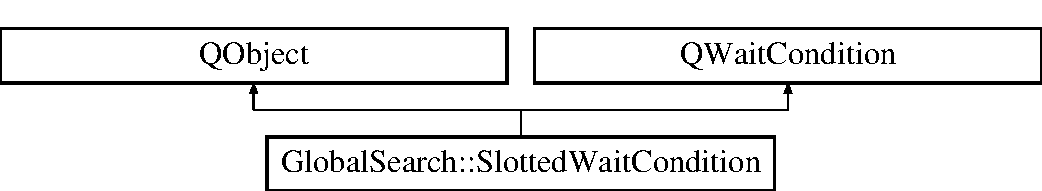
\includegraphics[height=2.000000cm]{classGlobalSearch_1_1SlottedWaitCondition}
\end{center}
\end{figure}
\subsection*{Public Slots}
\begin{DoxyCompactItemize}
\item 
void \hyperlink{classGlobalSearch_1_1SlottedWaitCondition_a26b060dde9c49345da5fe1c8dbd3374c}{wake\+One\+Slot} ()
\item 
void \hyperlink{classGlobalSearch_1_1SlottedWaitCondition_a4024066fe5db52f2e2c9257fcfbb5320}{wake\+All\+Slot} ()
\item 
void \hyperlink{classGlobalSearch_1_1SlottedWaitCondition_afb1ba4315ffa2de59eaf5045d2a4c09f}{prewait\+Lock} ()
\item 
void \hyperlink{classGlobalSearch_1_1SlottedWaitCondition_a3c9f9e3ba7eebdc3cc270445385e334c}{postwait\+Unlock} ()
\end{DoxyCompactItemize}
\subsection*{Public Member Functions}
\begin{DoxyCompactItemize}
\item 
\hyperlink{classGlobalSearch_1_1SlottedWaitCondition_a4fd4c5343242d8961fd893012ba9f54b}{Slotted\+Wait\+Condition} (Q\+Object $\ast$parent)
\item 
virtual \hyperlink{classGlobalSearch_1_1SlottedWaitCondition_a5b504c643c03b6b9e2e30e4a7613f43c}{$\sim$\+Slotted\+Wait\+Condition} ()
\item 
Q\+Mutex $\ast$ \hyperlink{classGlobalSearch_1_1SlottedWaitCondition_af548d9a604d2ec84083e5c92ca1a3849}{mutex} ()
\item 
void \hyperlink{classGlobalSearch_1_1SlottedWaitCondition_a30999486ab4737cda3c4e93f8625ac1f}{wait} (unsigned long timeout)
\end{DoxyCompactItemize}


\subsection{Detailed Description}
A wrapper for Q\+Wait\+Condition that has slots for wake\+One and wake\+All. See warning in expanded documentation. 

\begin{DoxyWarning}{Warning}
Misuse of this class can easily lead to a deadlock. If all calls to the wake$\ast$ slots are made before \hyperlink{classGlobalSearch_1_1SlottedWaitCondition_a30999486ab4737cda3c4e93f8625ac1f}{wait()} is called, the code may hang indefinitely. Ensure that \hyperlink{classGlobalSearch_1_1SlottedWaitCondition_a30999486ab4737cda3c4e93f8625ac1f}{wait()} is not called without setting a timeout to prevent this. For similar reasons, it is recommended that this construct is only used for trivial applications, such as G\+U\+I updates.
\end{DoxyWarning}
This class adds a few new functions to Q\+Wait\+Condition\+:
\begin{DoxyItemize}
\item \hyperlink{classGlobalSearch_1_1SlottedWaitCondition_a26b060dde9c49345da5fe1c8dbd3374c}{wake\+One\+Slot()}\+: A slot that calls Q\+Wait\+Condition\+::wake\+One()
\item \hyperlink{classGlobalSearch_1_1SlottedWaitCondition_a4024066fe5db52f2e2c9257fcfbb5320}{wake\+All\+Slot()}\+: A slot that calls Q\+Wait\+Condition\+::wake\+All()
\item \hyperlink{classGlobalSearch_1_1SlottedWaitCondition_af548d9a604d2ec84083e5c92ca1a3849}{mutex()}\+: Returns a pointer to the internal mutex (see below)
\item \hyperlink{classGlobalSearch_1_1SlottedWaitCondition_afb1ba4315ffa2de59eaf5045d2a4c09f}{prewait\+Lock()}\+: A slot that locks the internal mutex (see below)
\item \hyperlink{classGlobalSearch_1_1SlottedWaitCondition_a3c9f9e3ba7eebdc3cc270445385e334c}{postwait\+Unlock()}\+: A slot that unlocks the internal mutex (see below)
\end{DoxyItemize}

\hyperlink{classGlobalSearch_1_1SlottedWaitCondition}{Slotted\+Wait\+Condition} also includes an internal mutex that can be used for create critical sections before and after calls to \hyperlink{classGlobalSearch_1_1SlottedWaitCondition_a30999486ab4737cda3c4e93f8625ac1f}{wait()}. Normally an external mutex is used for this, but calls to \hyperlink{classGlobalSearch_1_1SlottedWaitCondition_a30999486ab4737cda3c4e93f8625ac1f}{wait()}, \hyperlink{classGlobalSearch_1_1SlottedWaitCondition_afb1ba4315ffa2de59eaf5045d2a4c09f}{prewait\+Lock()}, and \hyperlink{classGlobalSearch_1_1SlottedWaitCondition_a3c9f9e3ba7eebdc3cc270445385e334c}{postwait\+Unlock()} use the internal mutex. Calling \hyperlink{classGlobalSearch_1_1SlottedWaitCondition_af548d9a604d2ec84083e5c92ca1a3849}{mutex()} will return a pointer to this mutex. Typical usage of this wait condition is\+: 
\begin{DoxyCode}
\hyperlink{classGlobalSearch_1_1SlottedWaitCondition_a4fd4c5343242d8961fd893012ba9f54b}{SlottedWaitCondition} slottedWC;
...
connect(sender, SIGNAL(somethingThatFreesSlottedWCsResources()),
        &slottedWC, SLOT(\hyperlink{classGlobalSearch_1_1SlottedWaitCondition_a4024066fe5db52f2e2c9257fcfbb5320}{wakeAllSlot}()));

slottedWC->prewaitLock();
\textcolor{comment}{// Do any work that needs to be peformed in a critical section before waiting}
...

\textcolor{comment}{// Check every 250 milliseconds that we still need to be waiting}
while (someConditionIsTrue) \{
  slottedWC->wait(250);
\}

\textcolor{comment}{// Do any work that needs to be done in a critical section after waking}
...

slottedWC->postwaitUnlock();
\end{DoxyCode}
 \begin{DoxyVerb} @author David C. Lonie\end{DoxyVerb}
 

Definition at line 74 of file slottedwaitcondition.\+h.



\subsection{Constructor \& Destructor Documentation}
\hypertarget{classGlobalSearch_1_1SlottedWaitCondition_a4fd4c5343242d8961fd893012ba9f54b}{}\index{Global\+Search\+::\+Slotted\+Wait\+Condition@{Global\+Search\+::\+Slotted\+Wait\+Condition}!Slotted\+Wait\+Condition@{Slotted\+Wait\+Condition}}
\index{Slotted\+Wait\+Condition@{Slotted\+Wait\+Condition}!Global\+Search\+::\+Slotted\+Wait\+Condition@{Global\+Search\+::\+Slotted\+Wait\+Condition}}
\subsubsection[{Slotted\+Wait\+Condition}]{\setlength{\rightskip}{0pt plus 5cm}Global\+Search\+::\+Slotted\+Wait\+Condition\+::\+Slotted\+Wait\+Condition (
\begin{DoxyParamCaption}
\item[{Q\+Object $\ast$}]{parent}
\end{DoxyParamCaption}
)}\label{classGlobalSearch_1_1SlottedWaitCondition_a4fd4c5343242d8961fd893012ba9f54b}
Constructor.


\begin{DoxyParams}{Parameters}
{\em parent} & Parent for Q\+Object. \\
\hline
\end{DoxyParams}


Definition at line 20 of file slottedwaitcondition.\+cpp.

\hypertarget{classGlobalSearch_1_1SlottedWaitCondition_a5b504c643c03b6b9e2e30e4a7613f43c}{}\index{Global\+Search\+::\+Slotted\+Wait\+Condition@{Global\+Search\+::\+Slotted\+Wait\+Condition}!````~Slotted\+Wait\+Condition@{$\sim$\+Slotted\+Wait\+Condition}}
\index{````~Slotted\+Wait\+Condition@{$\sim$\+Slotted\+Wait\+Condition}!Global\+Search\+::\+Slotted\+Wait\+Condition@{Global\+Search\+::\+Slotted\+Wait\+Condition}}
\subsubsection[{$\sim$\+Slotted\+Wait\+Condition}]{\setlength{\rightskip}{0pt plus 5cm}Global\+Search\+::\+Slotted\+Wait\+Condition\+::$\sim$\+Slotted\+Wait\+Condition (
\begin{DoxyParamCaption}
{}
\end{DoxyParamCaption}
)\hspace{0.3cm}{\ttfamily [virtual]}}\label{classGlobalSearch_1_1SlottedWaitCondition_a5b504c643c03b6b9e2e30e4a7613f43c}
Destructor. 

Definition at line 27 of file slottedwaitcondition.\+cpp.



\subsection{Member Function Documentation}
\hypertarget{classGlobalSearch_1_1SlottedWaitCondition_af548d9a604d2ec84083e5c92ca1a3849}{}\index{Global\+Search\+::\+Slotted\+Wait\+Condition@{Global\+Search\+::\+Slotted\+Wait\+Condition}!mutex@{mutex}}
\index{mutex@{mutex}!Global\+Search\+::\+Slotted\+Wait\+Condition@{Global\+Search\+::\+Slotted\+Wait\+Condition}}
\subsubsection[{mutex}]{\setlength{\rightskip}{0pt plus 5cm}Q\+Mutex$\ast$ Global\+Search\+::\+Slotted\+Wait\+Condition\+::mutex (
\begin{DoxyParamCaption}
{}
\end{DoxyParamCaption}
)\hspace{0.3cm}{\ttfamily [inline]}}\label{classGlobalSearch_1_1SlottedWaitCondition_af548d9a604d2ec84083e5c92ca1a3849}
\begin{DoxyReturn}{Returns}
A pointer to the internal mutex, m\+\_\+mutex. 
\end{DoxyReturn}
\begin{DoxySeeAlso}{See also}
\hyperlink{classGlobalSearch_1_1SlottedWaitCondition_afb1ba4315ffa2de59eaf5045d2a4c09f}{prewait\+Lock} 

\hyperlink{classGlobalSearch_1_1SlottedWaitCondition_a3c9f9e3ba7eebdc3cc270445385e334c}{postwait\+Unlock} 

\hyperlink{classGlobalSearch_1_1SlottedWaitCondition_a30999486ab4737cda3c4e93f8625ac1f}{wait} 
\end{DoxySeeAlso}


Definition at line 108 of file slottedwaitcondition.\+h.

\hypertarget{classGlobalSearch_1_1SlottedWaitCondition_a3c9f9e3ba7eebdc3cc270445385e334c}{}\index{Global\+Search\+::\+Slotted\+Wait\+Condition@{Global\+Search\+::\+Slotted\+Wait\+Condition}!postwait\+Unlock@{postwait\+Unlock}}
\index{postwait\+Unlock@{postwait\+Unlock}!Global\+Search\+::\+Slotted\+Wait\+Condition@{Global\+Search\+::\+Slotted\+Wait\+Condition}}
\subsubsection[{postwait\+Unlock}]{\setlength{\rightskip}{0pt plus 5cm}void Global\+Search\+::\+Slotted\+Wait\+Condition\+::postwait\+Unlock (
\begin{DoxyParamCaption}
{}
\end{DoxyParamCaption}
)\hspace{0.3cm}{\ttfamily [inline]}, {\ttfamily [slot]}}\label{classGlobalSearch_1_1SlottedWaitCondition_a3c9f9e3ba7eebdc3cc270445385e334c}
Unlock the internal mutex, m\+\_\+mutex, to end the critical section after calling \hyperlink{classGlobalSearch_1_1SlottedWaitCondition_a30999486ab4737cda3c4e93f8625ac1f}{wait()}. 

Definition at line 159 of file slottedwaitcondition.\+h.

\hypertarget{classGlobalSearch_1_1SlottedWaitCondition_afb1ba4315ffa2de59eaf5045d2a4c09f}{}\index{Global\+Search\+::\+Slotted\+Wait\+Condition@{Global\+Search\+::\+Slotted\+Wait\+Condition}!prewait\+Lock@{prewait\+Lock}}
\index{prewait\+Lock@{prewait\+Lock}!Global\+Search\+::\+Slotted\+Wait\+Condition@{Global\+Search\+::\+Slotted\+Wait\+Condition}}
\subsubsection[{prewait\+Lock}]{\setlength{\rightskip}{0pt plus 5cm}void Global\+Search\+::\+Slotted\+Wait\+Condition\+::prewait\+Lock (
\begin{DoxyParamCaption}
{}
\end{DoxyParamCaption}
)\hspace{0.3cm}{\ttfamily [inline]}, {\ttfamily [slot]}}\label{classGlobalSearch_1_1SlottedWaitCondition_afb1ba4315ffa2de59eaf5045d2a4c09f}
Lock the internal mutex, m\+\_\+mutex, to create a critical section before calling \hyperlink{classGlobalSearch_1_1SlottedWaitCondition_a30999486ab4737cda3c4e93f8625ac1f}{wait()}. 

Definition at line 153 of file slottedwaitcondition.\+h.

\hypertarget{classGlobalSearch_1_1SlottedWaitCondition_a30999486ab4737cda3c4e93f8625ac1f}{}\index{Global\+Search\+::\+Slotted\+Wait\+Condition@{Global\+Search\+::\+Slotted\+Wait\+Condition}!wait@{wait}}
\index{wait@{wait}!Global\+Search\+::\+Slotted\+Wait\+Condition@{Global\+Search\+::\+Slotted\+Wait\+Condition}}
\subsubsection[{wait}]{\setlength{\rightskip}{0pt plus 5cm}void Global\+Search\+::\+Slotted\+Wait\+Condition\+::wait (
\begin{DoxyParamCaption}
\item[{unsigned long}]{timeout}
\end{DoxyParamCaption}
)\hspace{0.3cm}{\ttfamily [inline]}}\label{classGlobalSearch_1_1SlottedWaitCondition_a30999486ab4737cda3c4e93f8625ac1f}
Wait until woken up by one of\+:
\begin{DoxyItemize}
\item Q\+Wait\+Condition\+::wake\+One()
\item Q\+Wait\+Condition\+::wake\+All()
\item \hyperlink{classGlobalSearch_1_1SlottedWaitCondition_a26b060dde9c49345da5fe1c8dbd3374c}{Slotted\+Wait\+Condition\+::wake\+One\+Slot()}
\item \hyperlink{classGlobalSearch_1_1SlottedWaitCondition_a4024066fe5db52f2e2c9257fcfbb5320}{Slotted\+Wait\+Condition\+::wake\+All\+Slot()}
\end{DoxyItemize}

\begin{DoxyWarning}{Warning}
Misuse of this function can easily lead to a deadlock. If all calls to the wake$\ast$ slots are made before \hyperlink{classGlobalSearch_1_1SlottedWaitCondition_a30999486ab4737cda3c4e93f8625ac1f}{wait()} is called, the code may hang indefinitely. Ensure that \hyperlink{classGlobalSearch_1_1SlottedWaitCondition_a30999486ab4737cda3c4e93f8625ac1f}{wait()} is only called using a reasonable timeout to prevent this. For similar reasons, it is recommended that this construct is only used for trivial applications, such as G\+U\+I updates.
\end{DoxyWarning}

\begin{DoxyParams}{Parameters}
{\em timeout} & Timeout in milliseconds. After this time, the wait condition will wake itself and continue.\\
\hline
\end{DoxyParams}
This function expects the internal mutex, m\+\_\+mutex, to be locked before prior to using being called. This can be accomplished by calling lock() on \hyperlink{classGlobalSearch_1_1SlottedWaitCondition_af548d9a604d2ec84083e5c92ca1a3849}{mutex()} or \hyperlink{classGlobalSearch_1_1SlottedWaitCondition_afb1ba4315ffa2de59eaf5045d2a4c09f}{prewait\+Lock()}. The internal mutex will be locked before returning from this function. The mutex can be unlocked by calling the convenience function \hyperlink{classGlobalSearch_1_1SlottedWaitCondition_a3c9f9e3ba7eebdc3cc270445385e334c}{postwait\+Unlock()}. See class description for example usage. 

Definition at line 135 of file slottedwaitcondition.\+h.

\hypertarget{classGlobalSearch_1_1SlottedWaitCondition_a4024066fe5db52f2e2c9257fcfbb5320}{}\index{Global\+Search\+::\+Slotted\+Wait\+Condition@{Global\+Search\+::\+Slotted\+Wait\+Condition}!wake\+All\+Slot@{wake\+All\+Slot}}
\index{wake\+All\+Slot@{wake\+All\+Slot}!Global\+Search\+::\+Slotted\+Wait\+Condition@{Global\+Search\+::\+Slotted\+Wait\+Condition}}
\subsubsection[{wake\+All\+Slot}]{\setlength{\rightskip}{0pt plus 5cm}void Global\+Search\+::\+Slotted\+Wait\+Condition\+::wake\+All\+Slot (
\begin{DoxyParamCaption}
{}
\end{DoxyParamCaption}
)\hspace{0.3cm}{\ttfamily [inline]}, {\ttfamily [slot]}}\label{classGlobalSearch_1_1SlottedWaitCondition_a4024066fe5db52f2e2c9257fcfbb5320}
Slot that calls Q\+Wait\+Condition\+::wake\+All() 

Definition at line 147 of file slottedwaitcondition.\+h.

\hypertarget{classGlobalSearch_1_1SlottedWaitCondition_a26b060dde9c49345da5fe1c8dbd3374c}{}\index{Global\+Search\+::\+Slotted\+Wait\+Condition@{Global\+Search\+::\+Slotted\+Wait\+Condition}!wake\+One\+Slot@{wake\+One\+Slot}}
\index{wake\+One\+Slot@{wake\+One\+Slot}!Global\+Search\+::\+Slotted\+Wait\+Condition@{Global\+Search\+::\+Slotted\+Wait\+Condition}}
\subsubsection[{wake\+One\+Slot}]{\setlength{\rightskip}{0pt plus 5cm}void Global\+Search\+::\+Slotted\+Wait\+Condition\+::wake\+One\+Slot (
\begin{DoxyParamCaption}
{}
\end{DoxyParamCaption}
)\hspace{0.3cm}{\ttfamily [inline]}, {\ttfamily [slot]}}\label{classGlobalSearch_1_1SlottedWaitCondition_a26b060dde9c49345da5fe1c8dbd3374c}
Slot that calls Q\+Wait\+Condition\+::wake\+One() 

Definition at line 142 of file slottedwaitcondition.\+h.



The documentation for this class was generated from the following files\+:\begin{DoxyCompactItemize}
\item 
src/globalsearch/slottedwaitcondition.\+h\item 
src/globalsearch/slottedwaitcondition.\+cpp\end{DoxyCompactItemize}

\hypertarget{classGlobalSearch_1_1Structure}{\section{Global\-Search\-:\-:Structure Class Reference}
\label{classGlobalSearch_1_1Structure}\index{Global\-Search\-::\-Structure@{Global\-Search\-::\-Structure}}
}


Generic molecule object.  




{\ttfamily \#include $<$globalsearch/structure.\-h$>$}

Inheritance diagram for Global\-Search\-:\-:Structure\-:\begin{figure}[H]
\begin{center}
\leavevmode
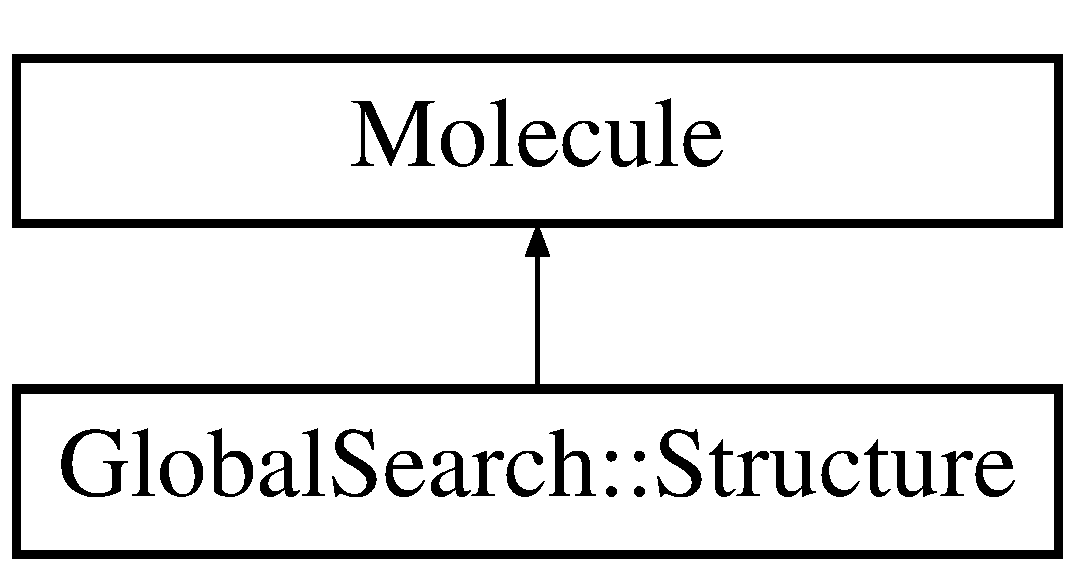
\includegraphics[height=2.000000cm]{classGlobalSearch_1_1Structure}
\end{center}
\end{figure}
\subsection*{Public Types}
\begin{DoxyCompactItemize}
\item 
enum \hyperlink{classGlobalSearch_1_1Structure_a3f1e44cb4f603fe1b3fbc8e813535917}{State} \{ \\*
\hyperlink{classGlobalSearch_1_1Structure_a3f1e44cb4f603fe1b3fbc8e813535917a75ed0969285b99dc1e54c654428be5e0}{Optimized} = 0, 
\hyperlink{classGlobalSearch_1_1Structure_a3f1e44cb4f603fe1b3fbc8e813535917ae572101eab4010061be0073888fbee39}{Step\-Optimized}, 
\hyperlink{classGlobalSearch_1_1Structure_a3f1e44cb4f603fe1b3fbc8e813535917ad4d8f76770421b6ab8d39f60e280a0a0}{Waiting\-For\-Optimization}, 
\hyperlink{classGlobalSearch_1_1Structure_a3f1e44cb4f603fe1b3fbc8e813535917a4f451a4c3de6ed294e1c7d06e5b1d24c}{In\-Process}, 
\\*
\hyperlink{classGlobalSearch_1_1Structure_a3f1e44cb4f603fe1b3fbc8e813535917a1639a0fd1ec7f1bba6cdaf73a2e76582}{Empty}, 
\hyperlink{classGlobalSearch_1_1Structure_a3f1e44cb4f603fe1b3fbc8e813535917ae64ed17fe917f0b8fd679078b5b12447}{Updating}, 
\hyperlink{classGlobalSearch_1_1Structure_a3f1e44cb4f603fe1b3fbc8e813535917a6b33b578b7e228f289720292019a998a}{Error}, 
\hyperlink{classGlobalSearch_1_1Structure_a3f1e44cb4f603fe1b3fbc8e813535917a5a0e4ad5830e2c3a9b045da79098b6c7}{Submitted}, 
\\*
\hyperlink{classGlobalSearch_1_1Structure_a3f1e44cb4f603fe1b3fbc8e813535917acd16cf0031d5e5b522b61618fd73fdc1}{Killed}, 
\hyperlink{classGlobalSearch_1_1Structure_a3f1e44cb4f603fe1b3fbc8e813535917ac5686d195648a0800584c59d034e8be0}{Removed}, 
\hyperlink{classGlobalSearch_1_1Structure_a3f1e44cb4f603fe1b3fbc8e813535917a1cd89f1eb6cab53ae2bb1b2ad64dfe72}{Duplicate}, 
\hyperlink{classGlobalSearch_1_1Structure_a3f1e44cb4f603fe1b3fbc8e813535917a99c42cb7635428e83d759cdae79209ec}{Restart}
 \}
\end{DoxyCompactItemize}
\subsection*{Public Slots}
\begin{DoxyCompactItemize}
\item 
virtual void \hyperlink{classGlobalSearch_1_1Structure_aff5394b9be0fa599c58f906d9a03f9d5}{setup\-Connections} ()
\item 
virtual void \hyperlink{classGlobalSearch_1_1Structure_a36f95cfbd571cce162a4bc59bb468f61}{enable\-Auto\-Histogram\-Generation} (bool)
\item 
virtual void \hyperlink{classGlobalSearch_1_1Structure_aaed562bf0ad4fe7bec1567eb84dbeee2}{request\-Histogram\-Generation} ()
\item 
virtual void \hyperlink{classGlobalSearch_1_1Structure_a57ae57cebf3df177a1363b91383a1c69}{generate\-Default\-Histogram} ()
\item 
virtual void \hyperlink{classGlobalSearch_1_1Structure_a1e30a18add5bd7e217546333262010ad}{structure\-Changed} ()
\item 
static bool \hyperlink{classGlobalSearch_1_1Structure_a92cca2b7d5a566d69dd228d267758c73}{compare\-I\-A\-D\-Distributions} (const std\-::vector$<$ double $>$ \&d, const std\-::vector$<$ double $>$ \&f1, const std\-::vector$<$ double $>$ \&f2, double decay, double smear, double $\ast$error)
\item 
static bool \hyperlink{classGlobalSearch_1_1Structure_a70f9ced5a098560bad9fe97d1bb6361a}{compare\-I\-A\-D\-Distributions} (const Q\-List$<$ double $>$ \&d, const Q\-List$<$ double $>$ \&f1, const Q\-List$<$ double $>$ \&f2, double decay, double smear, double $\ast$error)
\item 
static bool \hyperlink{classGlobalSearch_1_1Structure_aaed919f70884814f824aac01d619f004}{compare\-I\-A\-D\-Distributions} (const Q\-List$<$ Q\-Variant $>$ \&d, const Q\-List$<$ Q\-Variant $>$ \&f1, const Q\-List$<$ Q\-Variant $>$ \&f2, double decay, double smear, double $\ast$error)
\item 
virtual void \hyperlink{classGlobalSearch_1_1Structure_af6da83169c21363c545ef3ee01d891d3}{write\-Settings} (const Q\-String \&filename)
\item 
virtual void \hyperlink{classGlobalSearch_1_1Structure_a352a550ebb2c8e511e3ad400a98b1373}{read\-Settings} (const Q\-String \&filename)
\item 
virtual void \hyperlink{classGlobalSearch_1_1Structure_a29a46bef48b3c9045b6e87ca87c2c6cb}{update\-And\-Skip\-History} (const Q\-List$<$ unsigned int $>$ \&atomic\-Nums, const Q\-List$<$ Eigen\-::\-Vector3d $>$ \&coords, const double energy=0, const double enthalpy=0, const Eigen\-::\-Matrix3d \&cell=Eigen\-::\-Matrix3d\-::\-Zero())
\item 
virtual void \hyperlink{classGlobalSearch_1_1Structure_a9e200fa25c362859fdf2cecfd4cbaf06}{update\-And\-Add\-To\-History} (const Q\-List$<$ unsigned int $>$ \&atomic\-Nums, const Q\-List$<$ Eigen\-::\-Vector3d $>$ \&coords, const double energy=0, const double enthalpy=0, const Eigen\-::\-Matrix3d \&cell=Eigen\-::\-Matrix3d\-::\-Zero())
\item 
virtual void \hyperlink{classGlobalSearch_1_1Structure_ab1f8dc25ec23c06bd8edac7b0f719906}{delete\-From\-History} (unsigned int index)
\item 
virtual void \hyperlink{classGlobalSearch_1_1Structure_aaf7c1811bcc7f591e2f6bccd9e56e18f}{retrieve\-History\-Entry} (unsigned int index, Q\-List$<$ unsigned int $>$ $\ast$atomic\-Nums, Q\-List$<$ Eigen\-::\-Vector3d $>$ $\ast$coords, double $\ast$energy, double $\ast$enthalpy, Eigen\-::\-Matrix3d $\ast$cell)
\item 
virtual unsigned int \hyperlink{classGlobalSearch_1_1Structure_a92fb3f639890b9005c0559fcf843c45c}{size\-Of\-History} ()
\item 
void \hyperlink{classGlobalSearch_1_1Structure_a3f0ef2f62e4467c70044bbf3965b6a26}{set\-Enthalpy} (double enthalpy)
\item 
void \hyperlink{classGlobalSearch_1_1Structure_a4eda6eb8ce8080fae9fe91587039e748}{set\-P\-V} (double pv)
\item 
void \hyperlink{classGlobalSearch_1_1Structure_a947839b5088f6829b81ef7f9f9938b04}{reset\-Enthalpy} ()
\item 
void \hyperlink{classGlobalSearch_1_1Structure_aa3a2350ff9b13a7b84337f66a1d18cf5}{reset\-Energy} ()
\item 
void \hyperlink{classGlobalSearch_1_1Structure_a52962ac4b557250b84d27e90799d18d0}{set\-O\-B\-Energy} (const Q\-String \&ff=Q\-String(\char`\"{}U\-F\-F\char`\"{}))
\item 
void \hyperlink{classGlobalSearch_1_1Structure_a2c7020f0ea0bfb58f37dffc6e5d955be}{set\-Rank} (uint rank)
\item 
void \hyperlink{classGlobalSearch_1_1Structure_adbb752fe62009e8adbb55cc1fdef0de1}{set\-Job\-I\-D} (uint id)
\item 
void \hyperlink{classGlobalSearch_1_1Structure_a2c3d51c041d38d172f3169d8c8d31b45}{set\-Generation} (uint gen)
\item 
void \hyperlink{classGlobalSearch_1_1Structure_a9ecf515564a4063d37ab1d0a8eb14d11}{set\-I\-D\-Number} (uint id)
\item 
void \hyperlink{classGlobalSearch_1_1Structure_a9f25226379d189f1bfd9e4698585c2e9}{set\-Index} (int index)
\item 
void \hyperlink{classGlobalSearch_1_1Structure_a4d833bf522b24a31bfd983ae16e370fe}{set\-Parents} (const Q\-String \&p)
\item 
void \hyperlink{classGlobalSearch_1_1Structure_adc3f7486abf0ad3421d60f6a05f3106e}{set\-Rempath} (const Q\-String \&p)
\item 
void \hyperlink{classGlobalSearch_1_1Structure_aee38b5fe04ee88a4584b181fa8d0fbf9}{set\-Status} (\hyperlink{classGlobalSearch_1_1Structure_a3f1e44cb4f603fe1b3fbc8e813535917}{State} status)
\item 
void \hyperlink{classGlobalSearch_1_1Structure_a3aa37aac76ad5255e51a9113b3d64d40}{set\-Current\-Opt\-Step} (uint i)
\item 
void \hyperlink{classGlobalSearch_1_1Structure_a130a124d8cd7d440d4c902726492e41b}{set\-Fail\-Count} (uint count)
\item 
void \hyperlink{classGlobalSearch_1_1Structure_a27532f25313083bea490b3b6fa84c743}{reset\-Fail\-Count} ()
\item 
void \hyperlink{classGlobalSearch_1_1Structure_ab1ea99315ad11fc88f0941069f169f1a}{add\-Failure} ()
\item 
void \hyperlink{classGlobalSearch_1_1Structure_a59fe04ad733d7a770e3775339d71b8c3}{set\-Duplicate\-String} (const Q\-String \&s)
\item 
void \hyperlink{classGlobalSearch_1_1Structure_a266a812642a92c135ae5c65157d528d6}{set\-Changed\-Since\-Dup\-Checked} (bool b)
\item 
void \hyperlink{classGlobalSearch_1_1Structure_ae623efedfaa8980e5121199eec928298}{start\-Opt\-Timer} ()
\item 
void \hyperlink{classGlobalSearch_1_1Structure_a5f19c86d2e41ec95efd370e87049384f}{stop\-Opt\-Timer} ()
\item 
void \hyperlink{classGlobalSearch_1_1Structure_afc5507175ebfb4da413a5c40a2a8dfb3}{set\-Opt\-Timer\-Start} (const Q\-Date\-Time \&d)
\item 
void \hyperlink{classGlobalSearch_1_1Structure_a9ca3435fd1e634ddd665a5af63abc431}{set\-Opt\-Timer\-End} (const Q\-Date\-Time \&d)
\item 
virtual void \hyperlink{classGlobalSearch_1_1Structure_aa9ede9f516912b34000000caa849689c}{load} (Q\-Text\-Stream \&in)
\end{DoxyCompactItemize}
\subsection*{Public Member Functions}
\begin{DoxyCompactItemize}
\item 
\hyperlink{classGlobalSearch_1_1Structure_ab7e8a0041535442bca879148833831ac}{Structure} (Q\-Object $\ast$parent=0)
\item 
\hyperlink{classGlobalSearch_1_1Structure_ad5f2adb0f379ee6dde14984df3eb73bc}{Structure} (const \hyperlink{classGlobalSearch_1_1Structure}{Structure} \&other)
\item 
\hyperlink{classGlobalSearch_1_1Structure_a2630d5c42da1cd86bd0c3b7d79e69618}{Structure} (const Avogadro\-::\-Molecule \&other)
\item 
virtual \hyperlink{classGlobalSearch_1_1Structure_a29cc3acd03872d7641a2fd76a53e0491}{$\sim$\-Structure} ()
\item 
\hyperlink{classGlobalSearch_1_1Structure}{Structure} \& \hyperlink{classGlobalSearch_1_1Structure_a4b257e8547d62da1c2393c123da994f1}{operator=} (const \hyperlink{classGlobalSearch_1_1Structure}{Structure} \&other)
\item 
\hyperlink{classGlobalSearch_1_1Structure}{Structure} \& \hyperlink{classGlobalSearch_1_1Structure_a22737e6da3810566ad0b8c6b672e1214}{operator=} (const Avogadro\-::\-Molecule \&other)
\item 
\hyperlink{classGlobalSearch_1_1Structure}{Structure} \& \hyperlink{classGlobalSearch_1_1Structure_accb684b9686676fd61164f298460f195}{copy\-Structure} (const \hyperlink{classGlobalSearch_1_1Structure}{Structure} \&other)
\item 
bool \hyperlink{classGlobalSearch_1_1Structure_a6f963ec03dda49caa05f5eb8a9f19c39}{has\-Enthalpy} () const 
\item 
double \hyperlink{classGlobalSearch_1_1Structure_acc6db7487d8bbeacda3868734f4294bd}{get\-Energy} () const 
\item 
double \hyperlink{classGlobalSearch_1_1Structure_a45e5069495574ae2d4b73a1759b7326b}{get\-Enthalpy} () const 
\item 
double \hyperlink{classGlobalSearch_1_1Structure_a66f08d0683f89fa6791b5b7b9838955d}{get\-P\-V} () const 
\item 
uint \hyperlink{classGlobalSearch_1_1Structure_aad467ff9bf423156b7cc8df3a2fb7b13}{get\-Rank} () const 
\item 
uint \hyperlink{classGlobalSearch_1_1Structure_a6d044ecacb068406234a502d30664bea}{get\-Job\-I\-D} () const 
\item 
uint \hyperlink{classGlobalSearch_1_1Structure_a7caa9c46c88ac5711cf9d150bd0dcbd6}{get\-Generation} () const 
\item 
uint \hyperlink{classGlobalSearch_1_1Structure_afc86429da4b4d6673a8c33a58841905d}{get\-I\-D\-Number} () const 
\item 
int \hyperlink{classGlobalSearch_1_1Structure_a73f8f57a695b3bebdea8a8b3d75e4138}{get\-Index} () const 
\item 
Q\-String \hyperlink{classGlobalSearch_1_1Structure_a495b4fd01788d6d10b3d6b138784d52d}{get\-Duplicate\-String} () const 
\item 
Q\-String \hyperlink{classGlobalSearch_1_1Structure_a0b30437b5e6cc5e6f3de9c413aa04847}{get\-Parents} () const 
\item 
Q\-String \hyperlink{classGlobalSearch_1_1Structure_a9294a602bcf48745259368025434b796}{get\-Rempath} () const 
\item 
\hyperlink{classGlobalSearch_1_1Structure_a3f1e44cb4f603fe1b3fbc8e813535917}{State} \hyperlink{classGlobalSearch_1_1Structure_ad67c972a173cddc939e3adabf65dd72b}{get\-Status} () const 
\item 
uint \hyperlink{classGlobalSearch_1_1Structure_a955a416ce3d99e5ecc0a68c23e33824c}{get\-Current\-Opt\-Step} ()
\item 
uint \hyperlink{classGlobalSearch_1_1Structure_a39a044521e91f117be11fcf9a1a562b3}{get\-Fail\-Count} ()
\item 
Q\-Date\-Time \hyperlink{classGlobalSearch_1_1Structure_a17a4bd931cc52643bb89a19c9298fc7f}{get\-Opt\-Timer\-Start} () const 
\item 
Q\-Date\-Time \hyperlink{classGlobalSearch_1_1Structure_a720cde3d4eabbeca51fd41160a89fb70}{get\-Opt\-Timer\-End} () const 
\item 
Q\-String \hyperlink{classGlobalSearch_1_1Structure_a38b039e671cdcae7eab7b976c93255de}{get\-I\-D\-String} () const 
\item 
virtual Q\-String \hyperlink{classGlobalSearch_1_1Structure_a5f4dde0d82dbf949fffd514ccb9fd7ac}{get\-Results\-Header} () const 
\item 
virtual Q\-String \hyperlink{classGlobalSearch_1_1Structure_a28886a7dbbde4d7320ea05aa6c50c2e6}{get\-Results\-Entry} () const 
\item 
virtual bool \hyperlink{classGlobalSearch_1_1Structure_ad5d59a1e8739f9cec4c39ca6d576d22a}{get\-Nearest\-Neighbor\-Distances} (Q\-List$<$ double $>$ $\ast$list) const 
\item 
virtual bool \hyperlink{classGlobalSearch_1_1Structure_adee82bcb74af1c15bb91e5a9aa0e3849}{get\-Shortest\-Interatomic\-Distance} (double \&shortest) const 
\item 
virtual bool \hyperlink{classGlobalSearch_1_1Structure_af90032040343059ebbc91ac294a0a020}{get\-Nearest\-Neighbor\-Distance} (const double x, const double y, const double z, double \&shortest) const 
\item 
virtual bool \hyperlink{classGlobalSearch_1_1Structure_af7280b04c20689040bb7bc69005aef49}{get\-Nearest\-Neighbor\-Distance} (const Avogadro\-::\-Atom $\ast$atom, double \&shortest) const 
\item 
Q\-List$<$ Avogadro\-::\-Atom $\ast$ $>$ \hyperlink{classGlobalSearch_1_1Structure_a741bc226576a6aebdc72573afec08fe2}{get\-Neighbors} (const double x, const double y, const double z, const double cutoff, Q\-List$<$ double $>$ $\ast$distances=0) const 
\item 
Q\-List$<$ Avogadro\-::\-Atom $\ast$ $>$ \hyperlink{classGlobalSearch_1_1Structure_af84f72e94d8961a8804ff38b0c20b785}{get\-Neighbors} (const Avogadro\-::\-Atom $\ast$atom, const double cutoff, Q\-List$<$ double $>$ $\ast$distances=0) const 
\item 
virtual void \hyperlink{classGlobalSearch_1_1Structure_a668fcf6ecb33ad5fd3ef9963dd059ce0}{get\-Default\-Histogram} (Q\-List$<$ double $>$ $\ast$dist, Q\-List$<$ double $>$ $\ast$freq) const 
\item 
virtual void \hyperlink{classGlobalSearch_1_1Structure_a15748e6ccd1971f70dcf24d26a07388f}{get\-Default\-Histogram} (Q\-List$<$ Q\-Variant $>$ $\ast$dist, Q\-List$<$ Q\-Variant $>$ $\ast$freq) const 
\item 
virtual bool \hyperlink{classGlobalSearch_1_1Structure_a18edce7ebc0e1f5d0f939369a737c778}{is\-Histogram\-Generation\-Pending} () const 
\item 
virtual bool \hyperlink{classGlobalSearch_1_1Structure_a39c00be4b7081dea0963a9183c5d8d36}{generate\-I\-A\-D\-Histogram} (Q\-List$<$ double $>$ $\ast$distance, Q\-List$<$ double $>$ $\ast$frequency, double min=0.\-0, double max=10.\-0, double step=0.\-01, Avogadro\-::\-Atom $\ast$atom=0) const 
\item 
virtual bool \hyperlink{classGlobalSearch_1_1Structure_a6009cbdb3990eba689cbdd27aa0305ea}{generate\-I\-A\-D\-Histogram} (Q\-List$<$ Q\-Variant $>$ $\ast$distance, Q\-List$<$ Q\-Variant $>$ $\ast$frequency, double min=0.\-0, double max=10.\-0, double step=0.\-01, Avogadro\-::\-Atom $\ast$atom=0) const 
\item 
virtual bool \hyperlink{classGlobalSearch_1_1Structure_a8e0db651a3a48cd249f13f3ae0ca2b68}{add\-Atom\-Randomly} (uint atomic\-Number, double min\-I\-A\-D=0.\-0, double max\-I\-A\-D=0.\-0, int max\-Attempts=1000, Avogadro\-::\-Atom $\ast$$\ast$atom=0)
\item 
Q\-List$<$ Q\-String $>$ \hyperlink{classGlobalSearch_1_1Structure_ac49455f75d38a9f1779179dad2ba8815}{get\-Symbols} () const 
\item 
Q\-List$<$ uint $>$ \hyperlink{classGlobalSearch_1_1Structure_a447f0dd62f6546809d9b144bd971254f}{get\-Number\-Of\-Atoms\-Alpha} () const 
\item 
Q\-String \hyperlink{classGlobalSearch_1_1Structure_abd1f083a58dad102d0f0b3b3d89da2df}{get\-Opt\-Elapsed} () const 
\item 
virtual Q\-Hash$<$ Q\-String, Q\-Variant $>$ \hyperlink{classGlobalSearch_1_1Structure_afc441f647ad6f72bf415ea06a657220a}{get\-Fingerprint} () const 
\item 
bool \hyperlink{classGlobalSearch_1_1Structure_a30b8895da1515056a968ae9622c54408}{has\-Changed\-Since\-Dup\-Checked} ()
\end{DoxyCompactItemize}
\subsection*{Static Public Member Functions}
\begin{DoxyCompactItemize}
\item 
static void \hyperlink{classGlobalSearch_1_1Structure_a58d72124caf9401902f6a7653e0e7646}{sort\-By\-Enthalpy} (Q\-List$<$ \hyperlink{classGlobalSearch_1_1Structure}{Structure} $\ast$ $>$ $\ast$structures)
\item 
static void \hyperlink{classGlobalSearch_1_1Structure_af258714834ae664a9a563f1f0af4a883}{rank\-By\-Enthalpy} (const Q\-List$<$ \hyperlink{classGlobalSearch_1_1Structure}{Structure} $\ast$ $>$ \&structures)
\item 
static void \hyperlink{classGlobalSearch_1_1Structure_a742dbf63765f00c205657366f7e5efc8}{sort\-And\-Rank\-By\-Enthalpy} (Q\-List$<$ \hyperlink{classGlobalSearch_1_1Structure}{Structure} $\ast$ $>$ $\ast$structures)
\end{DoxyCompactItemize}
\subsection*{Protected Slots}
\begin{DoxyCompactItemize}
\item 
void \hyperlink{classGlobalSearch_1_1Structure_aa38396dff22066272e3b47604c9ac527}{write\-Structure\-Settings} (const Q\-String \&filename)
\item 
void \hyperlink{classGlobalSearch_1_1Structure_abe87722af78ae2e5913aebd7ae91ae6d}{read\-Structure\-Settings} (const Q\-String \&filename)
\end{DoxyCompactItemize}


\subsection{Detailed Description}
Generic molecule object. 

\begin{DoxyAuthor}{Author}
David C. Lonie
\end{DoxyAuthor}
The \hyperlink{classGlobalSearch_1_1Structure}{Structure} class provides a generic data object for storing information about a molecule. It derives from Avogadro\-::\-Molecule, adding new functionality to help with common tasks during a global structure search. 

Definition at line 48 of file structure.\-h.



\subsection{Member Enumeration Documentation}
\hypertarget{classGlobalSearch_1_1Structure_a3f1e44cb4f603fe1b3fbc8e813535917}{\index{Global\-Search\-::\-Structure@{Global\-Search\-::\-Structure}!State@{State}}
\index{State@{State}!GlobalSearch::Structure@{Global\-Search\-::\-Structure}}
\subsubsection[{State}]{\setlength{\rightskip}{0pt plus 5cm}enum {\bf Global\-Search\-::\-Structure\-::\-State}}}\label{classGlobalSearch_1_1Structure_a3f1e44cb4f603fe1b3fbc8e813535917}
Enum containing possible optimization statuses. \begin{DoxySeeAlso}{See Also}
\hyperlink{classGlobalSearch_1_1Structure_aee38b5fe04ee88a4584b181fa8d0fbf9}{set\-Status} 

\hyperlink{classGlobalSearch_1_1Structure_ad67c972a173cddc939e3adabf65dd72b}{get\-Status} 
\end{DoxySeeAlso}
\begin{Desc}
\item[Enumerator]\par
\begin{description}
\index{Optimized@{Optimized}!Global\-Search\-::\-Structure@{Global\-Search\-::\-Structure}}\index{Global\-Search\-::\-Structure@{Global\-Search\-::\-Structure}!Optimized@{Optimized}}\item[{\em 
\hypertarget{classGlobalSearch_1_1Structure_a3f1e44cb4f603fe1b3fbc8e813535917a75ed0969285b99dc1e54c654428be5e0}{Optimized}\label{classGlobalSearch_1_1Structure_a3f1e44cb4f603fe1b3fbc8e813535917a75ed0969285b99dc1e54c654428be5e0}
}]\hyperlink{classGlobalSearch_1_1Structure}{Structure} has completed all optimization steps \index{Step\-Optimized@{Step\-Optimized}!Global\-Search\-::\-Structure@{Global\-Search\-::\-Structure}}\index{Global\-Search\-::\-Structure@{Global\-Search\-::\-Structure}!Step\-Optimized@{Step\-Optimized}}\item[{\em 
\hypertarget{classGlobalSearch_1_1Structure_a3f1e44cb4f603fe1b3fbc8e813535917ae572101eab4010061be0073888fbee39}{Step\-Optimized}\label{classGlobalSearch_1_1Structure_a3f1e44cb4f603fe1b3fbc8e813535917ae572101eab4010061be0073888fbee39}
}]\hyperlink{classGlobalSearch_1_1Structure}{Structure} has completed an optimization step but may still have some to complete. \hyperlink{classGlobalSearch_1_1Structure_a955a416ce3d99e5ecc0a68c23e33824c}{get\-Current\-Opt\-Step()} shows the step that has just completed. \index{Waiting\-For\-Optimization@{Waiting\-For\-Optimization}!Global\-Search\-::\-Structure@{Global\-Search\-::\-Structure}}\index{Global\-Search\-::\-Structure@{Global\-Search\-::\-Structure}!Waiting\-For\-Optimization@{Waiting\-For\-Optimization}}\item[{\em 
\hypertarget{classGlobalSearch_1_1Structure_a3f1e44cb4f603fe1b3fbc8e813535917ad4d8f76770421b6ab8d39f60e280a0a0}{Waiting\-For\-Optimization}\label{classGlobalSearch_1_1Structure_a3f1e44cb4f603fe1b3fbc8e813535917ad4d8f76770421b6ab8d39f60e280a0a0}
}]\hyperlink{classGlobalSearch_1_1Structure}{Structure} is waiting to start an optimization step. \hyperlink{classGlobalSearch_1_1Structure_a955a416ce3d99e5ecc0a68c23e33824c}{get\-Current\-Opt\-Step()} shows the step it will start next. \index{In\-Process@{In\-Process}!Global\-Search\-::\-Structure@{Global\-Search\-::\-Structure}}\index{Global\-Search\-::\-Structure@{Global\-Search\-::\-Structure}!In\-Process@{In\-Process}}\item[{\em 
\hypertarget{classGlobalSearch_1_1Structure_a3f1e44cb4f603fe1b3fbc8e813535917a4f451a4c3de6ed294e1c7d06e5b1d24c}{In\-Process}\label{classGlobalSearch_1_1Structure_a3f1e44cb4f603fe1b3fbc8e813535917a4f451a4c3de6ed294e1c7d06e5b1d24c}
}]\hyperlink{classGlobalSearch_1_1Structure}{Structure} is currently queued or running an optimization step on the P\-B\-S server (if applicable). \index{Empty@{Empty}!Global\-Search\-::\-Structure@{Global\-Search\-::\-Structure}}\index{Global\-Search\-::\-Structure@{Global\-Search\-::\-Structure}!Empty@{Empty}}\item[{\em 
\hypertarget{classGlobalSearch_1_1Structure_a3f1e44cb4f603fe1b3fbc8e813535917a1639a0fd1ec7f1bba6cdaf73a2e76582}{Empty}\label{classGlobalSearch_1_1Structure_a3f1e44cb4f603fe1b3fbc8e813535917a1639a0fd1ec7f1bba6cdaf73a2e76582}
}]\hyperlink{classGlobalSearch_1_1Structure}{Structure} has just been generated, and has not yet been initialized \index{Updating@{Updating}!Global\-Search\-::\-Structure@{Global\-Search\-::\-Structure}}\index{Global\-Search\-::\-Structure@{Global\-Search\-::\-Structure}!Updating@{Updating}}\item[{\em 
\hypertarget{classGlobalSearch_1_1Structure_a3f1e44cb4f603fe1b3fbc8e813535917ae64ed17fe917f0b8fd679078b5b12447}{Updating}\label{classGlobalSearch_1_1Structure_a3f1e44cb4f603fe1b3fbc8e813535917ae64ed17fe917f0b8fd679078b5b12447}
}]The \hyperlink{classGlobalSearch_1_1Structure}{Structure} has completed it's current optimization step, and the results of the calculation are being transferred and applied. \index{Error@{Error}!Global\-Search\-::\-Structure@{Global\-Search\-::\-Structure}}\index{Global\-Search\-::\-Structure@{Global\-Search\-::\-Structure}!Error@{Error}}\item[{\em 
\hypertarget{classGlobalSearch_1_1Structure_a3f1e44cb4f603fe1b3fbc8e813535917a6b33b578b7e228f289720292019a998a}{Error}\label{classGlobalSearch_1_1Structure_a3f1e44cb4f603fe1b3fbc8e813535917a6b33b578b7e228f289720292019a998a}
}]The optimization is failing. \index{Submitted@{Submitted}!Global\-Search\-::\-Structure@{Global\-Search\-::\-Structure}}\index{Global\-Search\-::\-Structure@{Global\-Search\-::\-Structure}!Submitted@{Submitted}}\item[{\em 
\hypertarget{classGlobalSearch_1_1Structure_a3f1e44cb4f603fe1b3fbc8e813535917a5a0e4ad5830e2c3a9b045da79098b6c7}{Submitted}\label{classGlobalSearch_1_1Structure_a3f1e44cb4f603fe1b3fbc8e813535917a5a0e4ad5830e2c3a9b045da79098b6c7}
}]The \hyperlink{classGlobalSearch_1_1Structure}{Structure} has been submitted to the P\-B\-S server, but has not appeared in the queue yet. \index{Killed@{Killed}!Global\-Search\-::\-Structure@{Global\-Search\-::\-Structure}}\index{Global\-Search\-::\-Structure@{Global\-Search\-::\-Structure}!Killed@{Killed}}\item[{\em 
\hypertarget{classGlobalSearch_1_1Structure_a3f1e44cb4f603fe1b3fbc8e813535917acd16cf0031d5e5b522b61618fd73fdc1}{Killed}\label{classGlobalSearch_1_1Structure_a3f1e44cb4f603fe1b3fbc8e813535917acd16cf0031d5e5b522b61618fd73fdc1}
}]The \hyperlink{classGlobalSearch_1_1Structure}{Structure} has been killed before finishing all optimization steps. \index{Removed@{Removed}!Global\-Search\-::\-Structure@{Global\-Search\-::\-Structure}}\index{Global\-Search\-::\-Structure@{Global\-Search\-::\-Structure}!Removed@{Removed}}\item[{\em 
\hypertarget{classGlobalSearch_1_1Structure_a3f1e44cb4f603fe1b3fbc8e813535917ac5686d195648a0800584c59d034e8be0}{Removed}\label{classGlobalSearch_1_1Structure_a3f1e44cb4f603fe1b3fbc8e813535917ac5686d195648a0800584c59d034e8be0}
}]The \hyperlink{classGlobalSearch_1_1Structure}{Structure} has been killed after finishing all optimization steps. \index{Duplicate@{Duplicate}!Global\-Search\-::\-Structure@{Global\-Search\-::\-Structure}}\index{Global\-Search\-::\-Structure@{Global\-Search\-::\-Structure}!Duplicate@{Duplicate}}\item[{\em 
\hypertarget{classGlobalSearch_1_1Structure_a3f1e44cb4f603fe1b3fbc8e813535917a1cd89f1eb6cab53ae2bb1b2ad64dfe72}{Duplicate}\label{classGlobalSearch_1_1Structure_a3f1e44cb4f603fe1b3fbc8e813535917a1cd89f1eb6cab53ae2bb1b2ad64dfe72}
}]The \hyperlink{classGlobalSearch_1_1Structure}{Structure} has been found to be a duplicate of another. The other structure's information can be found in \hyperlink{classGlobalSearch_1_1Structure_a495b4fd01788d6d10b3d6b138784d52d}{get\-Duplicate\-String()}. \index{Restart@{Restart}!Global\-Search\-::\-Structure@{Global\-Search\-::\-Structure}}\index{Global\-Search\-::\-Structure@{Global\-Search\-::\-Structure}!Restart@{Restart}}\item[{\em 
\hypertarget{classGlobalSearch_1_1Structure_a3f1e44cb4f603fe1b3fbc8e813535917a99c42cb7635428e83d759cdae79209ec}{Restart}\label{classGlobalSearch_1_1Structure_a3f1e44cb4f603fe1b3fbc8e813535917a99c42cb7635428e83d759cdae79209ec}
}]The \hyperlink{classGlobalSearch_1_1Structure}{Structure} is about to restart it's current optimization step. \end{description}
\end{Desc}


Definition at line 102 of file structure.\-h.



\subsection{Constructor \& Destructor Documentation}
\hypertarget{classGlobalSearch_1_1Structure_ab7e8a0041535442bca879148833831ac}{\index{Global\-Search\-::\-Structure@{Global\-Search\-::\-Structure}!Structure@{Structure}}
\index{Structure@{Structure}!GlobalSearch::Structure@{Global\-Search\-::\-Structure}}
\subsubsection[{Structure}]{\setlength{\rightskip}{0pt plus 5cm}Global\-Search\-::\-Structure\-::\-Structure (
\begin{DoxyParamCaption}
\item[{Q\-Object $\ast$}]{parent = {\ttfamily 0}}
\end{DoxyParamCaption}
)}}\label{classGlobalSearch_1_1Structure_ab7e8a0041535442bca879148833831ac}
Constructor.


\begin{DoxyParams}{Parameters}
{\em parent} & The object parent. \\
\hline
\end{DoxyParams}


Definition at line 42 of file structure.\-cpp.



References Empty, reset\-Fail\-Count(), and set\-Status().

\hypertarget{classGlobalSearch_1_1Structure_ad5f2adb0f379ee6dde14984df3eb73bc}{\index{Global\-Search\-::\-Structure@{Global\-Search\-::\-Structure}!Structure@{Structure}}
\index{Structure@{Structure}!GlobalSearch::Structure@{Global\-Search\-::\-Structure}}
\subsubsection[{Structure}]{\setlength{\rightskip}{0pt plus 5cm}Global\-Search\-::\-Structure\-::\-Structure (
\begin{DoxyParamCaption}
\item[{const {\bf Structure} \&}]{other}
\end{DoxyParamCaption}
)}}\label{classGlobalSearch_1_1Structure_ad5f2adb0f379ee6dde14984df3eb73bc}
Copy constructor. 

Definition at line 61 of file structure.\-cpp.

\hypertarget{classGlobalSearch_1_1Structure_a2630d5c42da1cd86bd0c3b7d79e69618}{\index{Global\-Search\-::\-Structure@{Global\-Search\-::\-Structure}!Structure@{Structure}}
\index{Structure@{Structure}!GlobalSearch::Structure@{Global\-Search\-::\-Structure}}
\subsubsection[{Structure}]{\setlength{\rightskip}{0pt plus 5cm}Global\-Search\-::\-Structure\-::\-Structure (
\begin{DoxyParamCaption}
\item[{const Avogadro\-::\-Molecule \&}]{other}
\end{DoxyParamCaption}
)}}\label{classGlobalSearch_1_1Structure_a2630d5c42da1cd86bd0c3b7d79e69618}
Explicit copy constructor for Molecules. 

Definition at line 77 of file structure.\-cpp.

\hypertarget{classGlobalSearch_1_1Structure_a29cc3acd03872d7641a2fd76a53e0491}{\index{Global\-Search\-::\-Structure@{Global\-Search\-::\-Structure}!$\sim$\-Structure@{$\sim$\-Structure}}
\index{$\sim$\-Structure@{$\sim$\-Structure}!GlobalSearch::Structure@{Global\-Search\-::\-Structure}}
\subsubsection[{$\sim$\-Structure}]{\setlength{\rightskip}{0pt plus 5cm}Global\-Search\-::\-Structure\-::$\sim$\-Structure (
\begin{DoxyParamCaption}
{}
\end{DoxyParamCaption}
)\hspace{0.3cm}{\ttfamily [virtual]}}}\label{classGlobalSearch_1_1Structure_a29cc3acd03872d7641a2fd76a53e0491}
Destructor. 

Definition at line 189 of file structure.\-cpp.



\subsection{Member Function Documentation}
\hypertarget{classGlobalSearch_1_1Structure_a8e0db651a3a48cd249f13f3ae0ca2b68}{\index{Global\-Search\-::\-Structure@{Global\-Search\-::\-Structure}!add\-Atom\-Randomly@{add\-Atom\-Randomly}}
\index{add\-Atom\-Randomly@{add\-Atom\-Randomly}!GlobalSearch::Structure@{Global\-Search\-::\-Structure}}
\subsubsection[{add\-Atom\-Randomly}]{\setlength{\rightskip}{0pt plus 5cm}bool Global\-Search\-::\-Structure\-::add\-Atom\-Randomly (
\begin{DoxyParamCaption}
\item[{uint}]{atomic\-Number, }
\item[{double}]{min\-I\-A\-D = {\ttfamily 0.0}, }
\item[{double}]{max\-I\-A\-D = {\ttfamily 0.0}, }
\item[{int}]{max\-Attempts = {\ttfamily 1000}, }
\item[{Avogadro\-::\-Atom $\ast$$\ast$}]{atom = {\ttfamily 0}}
\end{DoxyParamCaption}
)\hspace{0.3cm}{\ttfamily [virtual]}}}\label{classGlobalSearch_1_1Structure_a8e0db651a3a48cd249f13f3ae0ca2b68}
Add an atom to a random position in the \hyperlink{classGlobalSearch_1_1Structure}{Structure}. If no other atoms exist in the \hyperlink{classGlobalSearch_1_1Structure}{Structure}, the new atom is placed at (0,0,0).

\begin{DoxyReturn}{Returns}
true if the atom was sucessfully added within the specified interatomic distances.
\end{DoxyReturn}

\begin{DoxyParams}{Parameters}
{\em atomic\-Number} & Atomic number of atom to add.\\
\hline
{\em min\-I\-A\-D} & Smallest interatomic distance allowed (N\-U\-L\-L or omit for no limit)\\
\hline
{\em max\-I\-A\-D} & Largest interatomic distance allowed (N\-U\-L\-L or omit for no limit)\\
\hline
{\em max\-Attempts} & Maximum number of tries before giving up.\\
\hline
{\em atom} & Returns a pointer to the new atom. \\
\hline
\end{DoxyParams}


Definition at line 591 of file structure.\-cpp.



References get\-Nearest\-Neighbor\-Distance().

\hypertarget{classGlobalSearch_1_1Structure_ab1ea99315ad11fc88f0941069f169f1a}{\index{Global\-Search\-::\-Structure@{Global\-Search\-::\-Structure}!add\-Failure@{add\-Failure}}
\index{add\-Failure@{add\-Failure}!GlobalSearch::Structure@{Global\-Search\-::\-Structure}}
\subsubsection[{add\-Failure}]{\setlength{\rightskip}{0pt plus 5cm}void Global\-Search\-::\-Structure\-::add\-Failure (
\begin{DoxyParamCaption}
{}
\end{DoxyParamCaption}
)\hspace{0.3cm}{\ttfamily [inline]}, {\ttfamily [slot]}}}\label{classGlobalSearch_1_1Structure_ab1ea99315ad11fc88f0941069f169f1a}
Increase the number of times this \hyperlink{classGlobalSearch_1_1Structure}{Structure} has failed the current optimization step by one.

\begin{DoxySeeAlso}{See Also}
\hyperlink{classGlobalSearch_1_1Structure_a27532f25313083bea490b3b6fa84c743}{reset\-Fail\-Count} 

\hyperlink{classGlobalSearch_1_1Structure_a130a124d8cd7d440d4c902726492e41b}{set\-Fail\-Count} 

\hyperlink{classGlobalSearch_1_1Structure_a39a044521e91f117be11fcf9a1a562b3}{get\-Fail\-Count} 
\end{DoxySeeAlso}


Definition at line 972 of file structure.\-h.



References get\-Fail\-Count(), and set\-Fail\-Count().

\hypertarget{classGlobalSearch_1_1Structure_a92cca2b7d5a566d69dd228d267758c73}{\index{Global\-Search\-::\-Structure@{Global\-Search\-::\-Structure}!compare\-I\-A\-D\-Distributions@{compare\-I\-A\-D\-Distributions}}
\index{compare\-I\-A\-D\-Distributions@{compare\-I\-A\-D\-Distributions}!GlobalSearch::Structure@{Global\-Search\-::\-Structure}}
\subsubsection[{compare\-I\-A\-D\-Distributions}]{\setlength{\rightskip}{0pt plus 5cm}bool Global\-Search\-::\-Structure\-::compare\-I\-A\-D\-Distributions (
\begin{DoxyParamCaption}
\item[{const std\-::vector$<$ double $>$ \&}]{d, }
\item[{const std\-::vector$<$ double $>$ \&}]{f1, }
\item[{const std\-::vector$<$ double $>$ \&}]{f2, }
\item[{double}]{decay, }
\item[{double}]{smear, }
\item[{double $\ast$}]{error}
\end{DoxyParamCaption}
)\hspace{0.3cm}{\ttfamily [static]}, {\ttfamily [slot]}}}\label{classGlobalSearch_1_1Structure_a92cca2b7d5a566d69dd228d267758c73}
Compare two I\-A\-D histograms.

Given two histograms over the same range with the same step, this function calculates an error value to measure the differences between the two. A boxcar smoothing is performed using a width of \char`\"{}smear\char`\"{}, and an optional weight can be applied. The weight is a standard exponential decay with a halflife of \char`\"{}decay\char`\"{}.


\begin{DoxyParams}{Parameters}
{\em d} & List of distances \\
\hline
{\em f1} & First list of frequencies \\
\hline
{\em f2} & Second list of frequencies \\
\hline
{\em decay} & Exponential decay parameter for lowering weight of large I\-A\-Ds \\
\hline
{\em smear} & Boxcar smoothing width in Angstroms \\
\hline
{\em error} & Return error value\\
\hline
\end{DoxyParams}
\begin{DoxyReturn}{Returns}
Whether or not the operation could be performed. 
\end{DoxyReturn}


Definition at line 966 of file structure.\-cpp.



Referenced by compare\-I\-A\-D\-Distributions().

\hypertarget{classGlobalSearch_1_1Structure_a70f9ced5a098560bad9fe97d1bb6361a}{\index{Global\-Search\-::\-Structure@{Global\-Search\-::\-Structure}!compare\-I\-A\-D\-Distributions@{compare\-I\-A\-D\-Distributions}}
\index{compare\-I\-A\-D\-Distributions@{compare\-I\-A\-D\-Distributions}!GlobalSearch::Structure@{Global\-Search\-::\-Structure}}
\subsubsection[{compare\-I\-A\-D\-Distributions}]{\setlength{\rightskip}{0pt plus 5cm}bool Global\-Search\-::\-Structure\-::compare\-I\-A\-D\-Distributions (
\begin{DoxyParamCaption}
\item[{const Q\-List$<$ double $>$ \&}]{d, }
\item[{const Q\-List$<$ double $>$ \&}]{f1, }
\item[{const Q\-List$<$ double $>$ \&}]{f2, }
\item[{double}]{decay, }
\item[{double}]{smear, }
\item[{double $\ast$}]{error}
\end{DoxyParamCaption}
)\hspace{0.3cm}{\ttfamily [static]}, {\ttfamily [slot]}}}\label{classGlobalSearch_1_1Structure_a70f9ced5a098560bad9fe97d1bb6361a}
Compare two I\-A\-D histograms.

Given two histograms over the same range with the same step, this function calculates an error value to measure the differences between the two. A boxcar smoothing is performed using a width of \char`\"{}smear\char`\"{}, and an optional weight can be applied. The weight is a standard exponential decay with a halflife of \char`\"{}decay\char`\"{}.


\begin{DoxyParams}{Parameters}
{\em d} & List of distances \\
\hline
{\em f1} & First list of frequencies \\
\hline
{\em f2} & Second list of frequencies \\
\hline
{\em decay} & Exponential decay parameter for lowering weight of large I\-A\-Ds \\
\hline
{\em smear} & Boxcar smoothing width in Angstroms \\
\hline
{\em error} & Return error value\\
\hline
\end{DoxyParams}
\begin{DoxyReturn}{Returns}
Whether or not the operation could be performed. 
\end{DoxyReturn}


Definition at line 1037 of file structure.\-cpp.



References compare\-I\-A\-D\-Distributions().

\hypertarget{classGlobalSearch_1_1Structure_aaed919f70884814f824aac01d619f004}{\index{Global\-Search\-::\-Structure@{Global\-Search\-::\-Structure}!compare\-I\-A\-D\-Distributions@{compare\-I\-A\-D\-Distributions}}
\index{compare\-I\-A\-D\-Distributions@{compare\-I\-A\-D\-Distributions}!GlobalSearch::Structure@{Global\-Search\-::\-Structure}}
\subsubsection[{compare\-I\-A\-D\-Distributions}]{\setlength{\rightskip}{0pt plus 5cm}bool Global\-Search\-::\-Structure\-::compare\-I\-A\-D\-Distributions (
\begin{DoxyParamCaption}
\item[{const Q\-List$<$ Q\-Variant $>$ \&}]{d, }
\item[{const Q\-List$<$ Q\-Variant $>$ \&}]{f1, }
\item[{const Q\-List$<$ Q\-Variant $>$ \&}]{f2, }
\item[{double}]{decay, }
\item[{double}]{smear, }
\item[{double $\ast$}]{error}
\end{DoxyParamCaption}
)\hspace{0.3cm}{\ttfamily [static]}, {\ttfamily [slot]}}}\label{classGlobalSearch_1_1Structure_aaed919f70884814f824aac01d619f004}
Compare two I\-A\-D histograms.

Given two histograms over the same range with the same step, this function calculates an error value to measure the differences between the two. A boxcar smoothing is performed using a width of \char`\"{}smear\char`\"{}, and an optional weight can be applied. The weight is a standard exponential decay with a halflife of \char`\"{}decay\char`\"{}.


\begin{DoxyParams}{Parameters}
{\em d} & List of distances \\
\hline
{\em f1} & First list of frequencies \\
\hline
{\em f2} & Second list of frequencies \\
\hline
{\em decay} & Exponential decay parameter for lowering weight of large I\-A\-Ds \\
\hline
{\em smear} & Boxcar smoothing width in Angstroms \\
\hline
{\em error} & Return error value\\
\hline
\end{DoxyParams}
\begin{DoxyReturn}{Returns}
Whether or not the operation could be performed. 
\end{DoxyReturn}


Definition at line 1058 of file structure.\-cpp.



References compare\-I\-A\-D\-Distributions().

\hypertarget{classGlobalSearch_1_1Structure_accb684b9686676fd61164f298460f195}{\index{Global\-Search\-::\-Structure@{Global\-Search\-::\-Structure}!copy\-Structure@{copy\-Structure}}
\index{copy\-Structure@{copy\-Structure}!GlobalSearch::Structure@{Global\-Search\-::\-Structure}}
\subsubsection[{copy\-Structure}]{\setlength{\rightskip}{0pt plus 5cm}{\bf Structure} \& Global\-Search\-::\-Structure\-::copy\-Structure (
\begin{DoxyParamCaption}
\item[{const {\bf Structure} \&}]{other}
\end{DoxyParamCaption}
)}}\label{classGlobalSearch_1_1Structure_accb684b9686676fd61164f298460f195}
Only update this structure's atoms, bonds, and residue information from {\itshape other}. \begin{DoxySeeAlso}{See Also}
operator= 
\end{DoxySeeAlso}


Definition at line 225 of file structure.\-cpp.



Referenced by operator=().

\hypertarget{classGlobalSearch_1_1Structure_ab1f8dc25ec23c06bd8edac7b0f719906}{\index{Global\-Search\-::\-Structure@{Global\-Search\-::\-Structure}!delete\-From\-History@{delete\-From\-History}}
\index{delete\-From\-History@{delete\-From\-History}!GlobalSearch::Structure@{Global\-Search\-::\-Structure}}
\subsubsection[{delete\-From\-History}]{\setlength{\rightskip}{0pt plus 5cm}void Global\-Search\-::\-Structure\-::delete\-From\-History (
\begin{DoxyParamCaption}
\item[{unsigned int}]{index}
\end{DoxyParamCaption}
)\hspace{0.3cm}{\ttfamily [virtual]}, {\ttfamily [slot]}}}\label{classGlobalSearch_1_1Structure_ab1f8dc25ec23c06bd8edac7b0f719906}

\begin{DoxyParams}{Parameters}
{\em index} & Index of entry to remove from structure's history. \\
\hline
\end{DoxyParams}


Definition at line 552 of file structure.\-cpp.



References size\-Of\-History().

\hypertarget{classGlobalSearch_1_1Structure_a36f95cfbd571cce162a4bc59bb468f61}{\index{Global\-Search\-::\-Structure@{Global\-Search\-::\-Structure}!enable\-Auto\-Histogram\-Generation@{enable\-Auto\-Histogram\-Generation}}
\index{enable\-Auto\-Histogram\-Generation@{enable\-Auto\-Histogram\-Generation}!GlobalSearch::Structure@{Global\-Search\-::\-Structure}}
\subsubsection[{enable\-Auto\-Histogram\-Generation}]{\setlength{\rightskip}{0pt plus 5cm}void Global\-Search\-::\-Structure\-::enable\-Auto\-Histogram\-Generation (
\begin{DoxyParamCaption}
\item[{bool}]{b}
\end{DoxyParamCaption}
)\hspace{0.3cm}{\ttfamily [virtual]}, {\ttfamily [slot]}}}\label{classGlobalSearch_1_1Structure_a36f95cfbd571cce162a4bc59bb468f61}
Set whether the default histogram generation should be performed (default is off) 

Definition at line 132 of file structure.\-cpp.



References request\-Histogram\-Generation().

\hypertarget{classGlobalSearch_1_1Structure_a57ae57cebf3df177a1363b91383a1c69}{\index{Global\-Search\-::\-Structure@{Global\-Search\-::\-Structure}!generate\-Default\-Histogram@{generate\-Default\-Histogram}}
\index{generate\-Default\-Histogram@{generate\-Default\-Histogram}!GlobalSearch::Structure@{Global\-Search\-::\-Structure}}
\subsubsection[{generate\-Default\-Histogram}]{\setlength{\rightskip}{0pt plus 5cm}void Global\-Search\-::\-Structure\-::generate\-Default\-Histogram (
\begin{DoxyParamCaption}
{}
\end{DoxyParamCaption}
)\hspace{0.3cm}{\ttfamily [virtual]}, {\ttfamily [slot]}}}\label{classGlobalSearch_1_1Structure_a57ae57cebf3df177a1363b91383a1c69}
Generate default histogram data (0\-:10 A, 0.\-01 A step) \begin{DoxySeeAlso}{See Also}
\hyperlink{classGlobalSearch_1_1Structure_a18edce7ebc0e1f5d0f939369a737c778}{is\-Histogram\-Generation\-Pending()} 

\hyperlink{classGlobalSearch_1_1Structure_a668fcf6ecb33ad5fd3ef9963dd059ce0}{get\-Default\-Histogram()} 
\end{DoxySeeAlso}


Definition at line 801 of file structure.\-cpp.



References generate\-I\-A\-D\-Histogram().



Referenced by request\-Histogram\-Generation().

\hypertarget{classGlobalSearch_1_1Structure_a39c00be4b7081dea0963a9183c5d8d36}{\index{Global\-Search\-::\-Structure@{Global\-Search\-::\-Structure}!generate\-I\-A\-D\-Histogram@{generate\-I\-A\-D\-Histogram}}
\index{generate\-I\-A\-D\-Histogram@{generate\-I\-A\-D\-Histogram}!GlobalSearch::Structure@{Global\-Search\-::\-Structure}}
\subsubsection[{generate\-I\-A\-D\-Histogram}]{\setlength{\rightskip}{0pt plus 5cm}bool Global\-Search\-::\-Structure\-::generate\-I\-A\-D\-Histogram (
\begin{DoxyParamCaption}
\item[{Q\-List$<$ double $>$ $\ast$}]{distance, }
\item[{Q\-List$<$ double $>$ $\ast$}]{frequency, }
\item[{double}]{min = {\ttfamily 0.0}, }
\item[{double}]{max = {\ttfamily 10.0}, }
\item[{double}]{step = {\ttfamily 0.01}, }
\item[{Avogadro\-::\-Atom $\ast$}]{atom = {\ttfamily 0}}
\end{DoxyParamCaption}
) const\hspace{0.3cm}{\ttfamily [virtual]}}}\label{classGlobalSearch_1_1Structure_a39c00be4b7081dea0963a9183c5d8d36}
Generate data for a histogram of the distances between all atoms, or between one atom and all others.

If the parameter atom is specified, the resulting data will represent the distance distribution between that atom and all others. If omitted (or N\-U\-L\-L), a histogram of all interatomic distances is calculated.

Useful for estimating the coordination number of an atom from a plot.

\begin{DoxyWarning}{Warning}
This algorithm is not thoroughly tested and should not be relied upon. It is merely an estimation.
\end{DoxyWarning}
\begin{DoxyReturn}{Returns}
true if the operation makes sense for this \hyperlink{classGlobalSearch_1_1Structure}{Structure}, false otherwise (i.\-e. fewer than one atom present)
\end{DoxyReturn}

\begin{DoxyParams}{Parameters}
{\em distance} & List of distance values for the histogram bins.\\
\hline
{\em frequency} & Number of Atoms within the corresponding distance bin.\\
\hline
{\em min} & Value of starting histogram distance. \\
\hline
{\em max} & Value of ending histogram distance. \\
\hline
{\em step} & Increment between bins. \\
\hline
{\em atom} & Optional\-: Atom to calculate distances from.\\
\hline
\end{DoxyParams}
\begin{DoxySeeAlso}{See Also}
\hyperlink{classGlobalSearch_1_1Structure_adee82bcb74af1c15bb91e5a9aa0e3849}{get\-Shortest\-Interatomic\-Distance} 

\hyperlink{classGlobalSearch_1_1Structure_aaed562bf0ad4fe7bec1567eb84dbeee2}{request\-Histogram\-Generation} 

\hyperlink{classGlobalSearch_1_1Structure_af90032040343059ebbc91ac294a0a020}{get\-Nearest\-Neighbor\-Distance} 
\end{DoxySeeAlso}


Definition at line 823 of file structure.\-cpp.



Referenced by generate\-Default\-Histogram().

\hypertarget{classGlobalSearch_1_1Structure_a6009cbdb3990eba689cbdd27aa0305ea}{\index{Global\-Search\-::\-Structure@{Global\-Search\-::\-Structure}!generate\-I\-A\-D\-Histogram@{generate\-I\-A\-D\-Histogram}}
\index{generate\-I\-A\-D\-Histogram@{generate\-I\-A\-D\-Histogram}!GlobalSearch::Structure@{Global\-Search\-::\-Structure}}
\subsubsection[{generate\-I\-A\-D\-Histogram}]{\setlength{\rightskip}{0pt plus 5cm}bool Global\-Search\-::\-Structure\-::generate\-I\-A\-D\-Histogram (
\begin{DoxyParamCaption}
\item[{Q\-List$<$ Q\-Variant $>$ $\ast$}]{distance, }
\item[{Q\-List$<$ Q\-Variant $>$ $\ast$}]{frequency, }
\item[{double}]{min = {\ttfamily 0.0}, }
\item[{double}]{max = {\ttfamily 10.0}, }
\item[{double}]{step = {\ttfamily 0.01}, }
\item[{Avogadro\-::\-Atom $\ast$}]{atom = {\ttfamily 0}}
\end{DoxyParamCaption}
) const\hspace{0.3cm}{\ttfamily [virtual]}}}\label{classGlobalSearch_1_1Structure_a6009cbdb3990eba689cbdd27aa0305ea}
Generate data for a histogram of the distances between all atoms, or between one atom and all others.

If the parameter atom is specified, the resulting data will represent the distance distribution between that atom and all others. If omitted (or N\-U\-L\-L), a histogram of all interatomic distances is calculated.

Useful for estimating the coordination number of an atom from a plot.

\begin{DoxyWarning}{Warning}
This algorithm is not thoroughly tested and should not be relied upon. It is merely an estimation.
\end{DoxyWarning}
\begin{DoxyReturn}{Returns}
true if the operation makes sense for this \hyperlink{classGlobalSearch_1_1Structure}{Structure}, false otherwise (i.\-e. fewer than one atom present)
\end{DoxyReturn}

\begin{DoxyParams}{Parameters}
{\em distance} & List of distance values for the histogram bins.\\
\hline
{\em frequency} & Number of Atoms within the corresponding distance bin.\\
\hline
{\em min} & Value of starting histogram distance. \\
\hline
{\em max} & Value of ending histogram distance. \\
\hline
{\em step} & Increment between bins. \\
\hline
{\em atom} & Optional\-: Atom to calculate distances from.\\
\hline
\end{DoxyParams}
\begin{DoxySeeAlso}{See Also}
\hyperlink{classGlobalSearch_1_1Structure_adee82bcb74af1c15bb91e5a9aa0e3849}{get\-Shortest\-Interatomic\-Distance} 

\hyperlink{classGlobalSearch_1_1Structure_aaed562bf0ad4fe7bec1567eb84dbeee2}{request\-Histogram\-Generation} 

\hyperlink{classGlobalSearch_1_1Structure_af90032040343059ebbc91ac294a0a020}{get\-Nearest\-Neighbor\-Distance} 
\end{DoxySeeAlso}


Definition at line 897 of file structure.\-cpp.

\hypertarget{classGlobalSearch_1_1Structure_a955a416ce3d99e5ecc0a68c23e33824c}{\index{Global\-Search\-::\-Structure@{Global\-Search\-::\-Structure}!get\-Current\-Opt\-Step@{get\-Current\-Opt\-Step}}
\index{get\-Current\-Opt\-Step@{get\-Current\-Opt\-Step}!GlobalSearch::Structure@{Global\-Search\-::\-Structure}}
\subsubsection[{get\-Current\-Opt\-Step}]{\setlength{\rightskip}{0pt plus 5cm}uint Global\-Search\-::\-Structure\-::get\-Current\-Opt\-Step (
\begin{DoxyParamCaption}
{}
\end{DoxyParamCaption}
)\hspace{0.3cm}{\ttfamily [inline]}}}\label{classGlobalSearch_1_1Structure_a955a416ce3d99e5ecc0a68c23e33824c}
\begin{DoxyReturn}{Returns}
The current optimization step of the \hyperlink{classGlobalSearch_1_1Structure}{Structure}. 
\end{DoxyReturn}
\begin{DoxySeeAlso}{See Also}
\hyperlink{classGlobalSearch_1_1Structure_a3aa37aac76ad5255e51a9113b3d64d40}{set\-Current\-Opt\-Step} 
\end{DoxySeeAlso}


Definition at line 279 of file structure.\-h.



Referenced by Global\-Search\-::\-Optimizer\-::get\-Interpreted\-Templates(), Global\-Search\-::\-Opt\-Base\-::interpret\-Keyword\-\_\-base(), Global\-Search\-::\-Queue\-Manager\-::start\-Job(), and write\-Structure\-Settings().

\hypertarget{classGlobalSearch_1_1Structure_a668fcf6ecb33ad5fd3ef9963dd059ce0}{\index{Global\-Search\-::\-Structure@{Global\-Search\-::\-Structure}!get\-Default\-Histogram@{get\-Default\-Histogram}}
\index{get\-Default\-Histogram@{get\-Default\-Histogram}!GlobalSearch::Structure@{Global\-Search\-::\-Structure}}
\subsubsection[{get\-Default\-Histogram}]{\setlength{\rightskip}{0pt plus 5cm}void Global\-Search\-::\-Structure\-::get\-Default\-Histogram (
\begin{DoxyParamCaption}
\item[{Q\-List$<$ double $>$ $\ast$}]{dist, }
\item[{Q\-List$<$ double $>$ $\ast$}]{freq}
\end{DoxyParamCaption}
) const\hspace{0.3cm}{\ttfamily [virtual]}}}\label{classGlobalSearch_1_1Structure_a668fcf6ecb33ad5fd3ef9963dd059ce0}
Get the default histogram data. 

Definition at line 807 of file structure.\-cpp.

\hypertarget{classGlobalSearch_1_1Structure_a15748e6ccd1971f70dcf24d26a07388f}{\index{Global\-Search\-::\-Structure@{Global\-Search\-::\-Structure}!get\-Default\-Histogram@{get\-Default\-Histogram}}
\index{get\-Default\-Histogram@{get\-Default\-Histogram}!GlobalSearch::Structure@{Global\-Search\-::\-Structure}}
\subsubsection[{get\-Default\-Histogram}]{\setlength{\rightskip}{0pt plus 5cm}void Global\-Search\-::\-Structure\-::get\-Default\-Histogram (
\begin{DoxyParamCaption}
\item[{Q\-List$<$ Q\-Variant $>$ $\ast$}]{dist, }
\item[{Q\-List$<$ Q\-Variant $>$ $\ast$}]{freq}
\end{DoxyParamCaption}
) const\hspace{0.3cm}{\ttfamily [virtual]}}}\label{classGlobalSearch_1_1Structure_a15748e6ccd1971f70dcf24d26a07388f}
Get the default histogram data. 

Definition at line 817 of file structure.\-cpp.

\hypertarget{classGlobalSearch_1_1Structure_a495b4fd01788d6d10b3d6b138784d52d}{\index{Global\-Search\-::\-Structure@{Global\-Search\-::\-Structure}!get\-Duplicate\-String@{get\-Duplicate\-String}}
\index{get\-Duplicate\-String@{get\-Duplicate\-String}!GlobalSearch::Structure@{Global\-Search\-::\-Structure}}
\subsubsection[{get\-Duplicate\-String}]{\setlength{\rightskip}{0pt plus 5cm}Q\-String Global\-Search\-::\-Structure\-::get\-Duplicate\-String (
\begin{DoxyParamCaption}
{}
\end{DoxyParamCaption}
) const\hspace{0.3cm}{\ttfamily [inline]}}}\label{classGlobalSearch_1_1Structure_a495b4fd01788d6d10b3d6b138784d52d}
\begin{DoxyReturn}{Returns}
A string naming the \hyperlink{classGlobalSearch_1_1Structure}{Structure} that this \hyperlink{classGlobalSearch_1_1Structure}{Structure} is a duplicate of. 
\end{DoxyReturn}
\begin{DoxySeeAlso}{See Also}
\hyperlink{classGlobalSearch_1_1Structure_a59fe04ad733d7a770e3775339d71b8c3}{set\-Duplicate\-String} 
\end{DoxySeeAlso}


Definition at line 257 of file structure.\-h.

\hypertarget{classGlobalSearch_1_1Structure_acc6db7487d8bbeacda3868734f4294bd}{\index{Global\-Search\-::\-Structure@{Global\-Search\-::\-Structure}!get\-Energy@{get\-Energy}}
\index{get\-Energy@{get\-Energy}!GlobalSearch::Structure@{Global\-Search\-::\-Structure}}
\subsubsection[{get\-Energy}]{\setlength{\rightskip}{0pt plus 5cm}double Global\-Search\-::\-Structure\-::get\-Energy (
\begin{DoxyParamCaption}
{}
\end{DoxyParamCaption}
) const\hspace{0.3cm}{\ttfamily [inline]}}}\label{classGlobalSearch_1_1Structure_acc6db7487d8bbeacda3868734f4294bd}
Return the energy value of the first conformer in e\-V. This is a convenience function.

\begin{DoxyNote}{Note}
The energies of the other conformers are still available using energy(int). Be aware that energy(int) returns kcal/mol. The multiplicative factor E\-V\-\_\-\-T\-O\-\_\-\-K\-C\-A\-L\-\_\-\-P\-E\-R\-\_\-\-M\-O\-L has been defined to aid conversion.
\end{DoxyNote}
\begin{DoxyReturn}{Returns}
The energy of the first conformer in e\-V. 
\end{DoxyReturn}
\begin{DoxySeeAlso}{See Also}
\hyperlink{classGlobalSearch_1_1Structure_a3f0ef2f62e4467c70044bbf3965b6a26}{set\-Enthalpy} 

\hyperlink{classGlobalSearch_1_1Structure_a6f963ec03dda49caa05f5eb8a9f19c39}{has\-Enthalpy} 

\hyperlink{classGlobalSearch_1_1Structure_a4eda6eb8ce8080fae9fe91587039e748}{set\-P\-V} 

\hyperlink{classGlobalSearch_1_1Structure_a66f08d0683f89fa6791b5b7b9838955d}{get\-P\-V} 

set\-Energy 

\hyperlink{classGlobalSearch_1_1Structure_acc6db7487d8bbeacda3868734f4294bd}{get\-Energy} 
\end{DoxySeeAlso}


Definition at line 170 of file structure.\-h.



Referenced by get\-Enthalpy().

\hypertarget{classGlobalSearch_1_1Structure_a45e5069495574ae2d4b73a1759b7326b}{\index{Global\-Search\-::\-Structure@{Global\-Search\-::\-Structure}!get\-Enthalpy@{get\-Enthalpy}}
\index{get\-Enthalpy@{get\-Enthalpy}!GlobalSearch::Structure@{Global\-Search\-::\-Structure}}
\subsubsection[{get\-Enthalpy}]{\setlength{\rightskip}{0pt plus 5cm}double Global\-Search\-::\-Structure\-::get\-Enthalpy (
\begin{DoxyParamCaption}
{}
\end{DoxyParamCaption}
) const\hspace{0.3cm}{\ttfamily [inline]}}}\label{classGlobalSearch_1_1Structure_a45e5069495574ae2d4b73a1759b7326b}
Return the enthalpy value of the first conformer in e\-V.

\begin{DoxyNote}{Note}
If the enthalpy is not set but the energy is set, this function assumes that the system is at zero-\/pressure and returns the energy.
\end{DoxyNote}
\begin{DoxyReturn}{Returns}
The enthalpy of the first conformer in e\-V. 
\end{DoxyReturn}
\begin{DoxySeeAlso}{See Also}
\hyperlink{classGlobalSearch_1_1Structure_a3f0ef2f62e4467c70044bbf3965b6a26}{set\-Enthalpy} 

\hyperlink{classGlobalSearch_1_1Structure_a6f963ec03dda49caa05f5eb8a9f19c39}{has\-Enthalpy} 

\hyperlink{classGlobalSearch_1_1Structure_a4eda6eb8ce8080fae9fe91587039e748}{set\-P\-V} 

\hyperlink{classGlobalSearch_1_1Structure_a66f08d0683f89fa6791b5b7b9838955d}{get\-P\-V} 

set\-Energy 

\hyperlink{classGlobalSearch_1_1Structure_acc6db7487d8bbeacda3868734f4294bd}{get\-Energy} 
\end{DoxySeeAlso}


Definition at line 186 of file structure.\-h.



References get\-Energy().



Referenced by get\-Fingerprint(), Global\-Search\-::\-Opt\-Base\-::get\-Probability\-List(), get\-Results\-Entry(), rank\-By\-Enthalpy(), and sort\-By\-Enthalpy().

\hypertarget{classGlobalSearch_1_1Structure_a39a044521e91f117be11fcf9a1a562b3}{\index{Global\-Search\-::\-Structure@{Global\-Search\-::\-Structure}!get\-Fail\-Count@{get\-Fail\-Count}}
\index{get\-Fail\-Count@{get\-Fail\-Count}!GlobalSearch::Structure@{Global\-Search\-::\-Structure}}
\subsubsection[{get\-Fail\-Count}]{\setlength{\rightskip}{0pt plus 5cm}uint Global\-Search\-::\-Structure\-::get\-Fail\-Count (
\begin{DoxyParamCaption}
{}
\end{DoxyParamCaption}
)\hspace{0.3cm}{\ttfamily [inline]}}}\label{classGlobalSearch_1_1Structure_a39a044521e91f117be11fcf9a1a562b3}
\begin{DoxyReturn}{Returns}
The number of times this \hyperlink{classGlobalSearch_1_1Structure}{Structure} has failed the current optimization step. 
\end{DoxyReturn}
\begin{DoxySeeAlso}{See Also}
\hyperlink{classGlobalSearch_1_1Structure_a130a124d8cd7d440d4c902726492e41b}{set\-Fail\-Count} 

\hyperlink{classGlobalSearch_1_1Structure_ab1ea99315ad11fc88f0941069f169f1a}{add\-Failure} 

\hyperlink{classGlobalSearch_1_1Structure_a27532f25313083bea490b3b6fa84c743}{reset\-Fail\-Count} 
\end{DoxySeeAlso}


Definition at line 287 of file structure.\-h.



Referenced by add\-Failure(), Global\-Search\-::\-Queue\-Manager\-::check\-Population(), and write\-Structure\-Settings().

\hypertarget{classGlobalSearch_1_1Structure_afc441f647ad6f72bf415ea06a657220a}{\index{Global\-Search\-::\-Structure@{Global\-Search\-::\-Structure}!get\-Fingerprint@{get\-Fingerprint}}
\index{get\-Fingerprint@{get\-Fingerprint}!GlobalSearch::Structure@{Global\-Search\-::\-Structure}}
\subsubsection[{get\-Fingerprint}]{\setlength{\rightskip}{0pt plus 5cm}Q\-Hash$<$ Q\-String, Q\-Variant $>$ Global\-Search\-::\-Structure\-::get\-Fingerprint (
\begin{DoxyParamCaption}
{}
\end{DoxyParamCaption}
) const\hspace{0.3cm}{\ttfamily [virtual]}}}\label{classGlobalSearch_1_1Structure_afc441f647ad6f72bf415ea06a657220a}
A \char`\"{}fingerprint\char`\"{} hash of the structure. Returns \char`\"{}enthalpy\char`\"{} key with the enthalpy value as a double wrapped in a Q\-Variant. May be extended in derived classes.

Used for checking if two Structures are similar enough to be marked as duplicates.

\begin{DoxyReturn}{Returns}
A hash of key/value pairs containing data that is representative of the \hyperlink{classGlobalSearch_1_1Structure}{Structure}. 
\end{DoxyReturn}


Definition at line 1181 of file structure.\-cpp.



References get\-Enthalpy().

\hypertarget{classGlobalSearch_1_1Structure_a7caa9c46c88ac5711cf9d150bd0dcbd6}{\index{Global\-Search\-::\-Structure@{Global\-Search\-::\-Structure}!get\-Generation@{get\-Generation}}
\index{get\-Generation@{get\-Generation}!GlobalSearch::Structure@{Global\-Search\-::\-Structure}}
\subsubsection[{get\-Generation}]{\setlength{\rightskip}{0pt plus 5cm}uint Global\-Search\-::\-Structure\-::get\-Generation (
\begin{DoxyParamCaption}
{}
\end{DoxyParamCaption}
) const\hspace{0.3cm}{\ttfamily [inline]}}}\label{classGlobalSearch_1_1Structure_a7caa9c46c88ac5711cf9d150bd0dcbd6}
Returns the generation number of the structure. Only useful for genetic/evolutionary algorithms. \begin{DoxyReturn}{Returns}
Generation number 
\end{DoxyReturn}
\begin{DoxySeeAlso}{See Also}
\hyperlink{classGlobalSearch_1_1Structure_a2c3d51c041d38d172f3169d8c8d31b45}{set\-Generation} 

\hyperlink{classGlobalSearch_1_1Structure_afc86429da4b4d6673a8c33a58841905d}{get\-I\-D\-Number} 

\hyperlink{classGlobalSearch_1_1Structure_a73f8f57a695b3bebdea8a8b3d75e4138}{get\-Index} 

\hyperlink{classGlobalSearch_1_1Structure_a9ecf515564a4063d37ab1d0a8eb14d11}{set\-I\-D\-Number} 

\hyperlink{classGlobalSearch_1_1Structure_a9f25226379d189f1bfd9e4698585c2e9}{set\-Index} 

\hyperlink{classGlobalSearch_1_1Structure_a38b039e671cdcae7eab7b976c93255de}{get\-I\-D\-String} 
\end{DoxySeeAlso}


Definition at line 224 of file structure.\-h.



Referenced by get\-I\-D\-String(), get\-Results\-Entry(), Global\-Search\-::\-Opt\-Base\-::interpret\-Keyword\-\_\-base(), and write\-Structure\-Settings().

\hypertarget{classGlobalSearch_1_1Structure_afc86429da4b4d6673a8c33a58841905d}{\index{Global\-Search\-::\-Structure@{Global\-Search\-::\-Structure}!get\-I\-D\-Number@{get\-I\-D\-Number}}
\index{get\-I\-D\-Number@{get\-I\-D\-Number}!GlobalSearch::Structure@{Global\-Search\-::\-Structure}}
\subsubsection[{get\-I\-D\-Number}]{\setlength{\rightskip}{0pt plus 5cm}uint Global\-Search\-::\-Structure\-::get\-I\-D\-Number (
\begin{DoxyParamCaption}
{}
\end{DoxyParamCaption}
) const\hspace{0.3cm}{\ttfamily [inline]}}}\label{classGlobalSearch_1_1Structure_afc86429da4b4d6673a8c33a58841905d}
Returns an I\-D number associated with the \hyperlink{classGlobalSearch_1_1Structure}{Structure}.

\begin{DoxyNote}{Note}
If a generation number is used as well, this may not be unique. 
\end{DoxyNote}
\begin{DoxyReturn}{Returns}
Identification number 
\end{DoxyReturn}
\begin{DoxySeeAlso}{See Also}
\hyperlink{classGlobalSearch_1_1Structure_a2c3d51c041d38d172f3169d8c8d31b45}{set\-Generation} 

\hyperlink{classGlobalSearch_1_1Structure_a7caa9c46c88ac5711cf9d150bd0dcbd6}{get\-Generation} 

\hyperlink{classGlobalSearch_1_1Structure_a73f8f57a695b3bebdea8a8b3d75e4138}{get\-Index} 

\hyperlink{classGlobalSearch_1_1Structure_a9ecf515564a4063d37ab1d0a8eb14d11}{set\-I\-D\-Number} 

\hyperlink{classGlobalSearch_1_1Structure_a9f25226379d189f1bfd9e4698585c2e9}{set\-Index} 

\hyperlink{classGlobalSearch_1_1Structure_a38b039e671cdcae7eab7b976c93255de}{get\-I\-D\-String} 
\end{DoxySeeAlso}


Definition at line 238 of file structure.\-h.



Referenced by get\-I\-D\-String(), get\-Results\-Entry(), Global\-Search\-::\-Opt\-Base\-::interpret\-Keyword\-\_\-base(), and write\-Structure\-Settings().

\hypertarget{classGlobalSearch_1_1Structure_a38b039e671cdcae7eab7b976c93255de}{\index{Global\-Search\-::\-Structure@{Global\-Search\-::\-Structure}!get\-I\-D\-String@{get\-I\-D\-String}}
\index{get\-I\-D\-String@{get\-I\-D\-String}!GlobalSearch::Structure@{Global\-Search\-::\-Structure}}
\subsubsection[{get\-I\-D\-String}]{\setlength{\rightskip}{0pt plus 5cm}Q\-String Global\-Search\-::\-Structure\-::get\-I\-D\-String (
\begin{DoxyParamCaption}
{}
\end{DoxyParamCaption}
) const\hspace{0.3cm}{\ttfamily [inline]}}}\label{classGlobalSearch_1_1Structure_a38b039e671cdcae7eab7b976c93255de}
Returns a unique identification string. Defaults to \mbox{[}generation\mbox{]}x\mbox{[}I\-D\-Number\mbox{]}. Handy for debugging/error output. \begin{DoxyReturn}{Returns}
Unique identification string. 
\end{DoxyReturn}
\begin{DoxySeeAlso}{See Also}
\hyperlink{classGlobalSearch_1_1Structure_a2c3d51c041d38d172f3169d8c8d31b45}{set\-Generation} 

\hyperlink{classGlobalSearch_1_1Structure_a7caa9c46c88ac5711cf9d150bd0dcbd6}{get\-Generation} 

\hyperlink{classGlobalSearch_1_1Structure_a9f25226379d189f1bfd9e4698585c2e9}{set\-Index} 

\hyperlink{classGlobalSearch_1_1Structure_a73f8f57a695b3bebdea8a8b3d75e4138}{get\-Index} 

\hyperlink{classGlobalSearch_1_1Structure_a9ecf515564a4063d37ab1d0a8eb14d11}{set\-I\-D\-Number} 

\hyperlink{classGlobalSearch_1_1Structure_afc86429da4b4d6673a8c33a58841905d}{get\-I\-D\-Number} 
\end{DoxySeeAlso}


Definition at line 319 of file structure.\-h.



References get\-Generation(), and get\-I\-D\-Number().



Referenced by Global\-Search\-::\-Optimizer\-::get\-Interpreted\-Templates(), Global\-Search\-::\-Local\-Queue\-Interface\-::get\-Status(), Global\-Search\-::\-Optimizer\-::read(), Global\-Search\-::\-Local\-Queue\-Interface\-::start\-Job(), Global\-Search\-::\-Queue\-Manager\-::start\-Job(), Global\-Search\-::\-Queue\-Manager\-::unlock\-For\-Naming(), and Global\-Search\-::\-Optimizer\-::update().

\hypertarget{classGlobalSearch_1_1Structure_a73f8f57a695b3bebdea8a8b3d75e4138}{\index{Global\-Search\-::\-Structure@{Global\-Search\-::\-Structure}!get\-Index@{get\-Index}}
\index{get\-Index@{get\-Index}!GlobalSearch::Structure@{Global\-Search\-::\-Structure}}
\subsubsection[{get\-Index}]{\setlength{\rightskip}{0pt plus 5cm}int Global\-Search\-::\-Structure\-::get\-Index (
\begin{DoxyParamCaption}
{}
\end{DoxyParamCaption}
) const\hspace{0.3cm}{\ttfamily [inline]}}}\label{classGlobalSearch_1_1Structure_a73f8f57a695b3bebdea8a8b3d75e4138}
Returns a unique I\-D number associated with the \hyperlink{classGlobalSearch_1_1Structure}{Structure}. This is typically assigned in order of introduction to a tracker.

\begin{DoxyReturn}{Returns}
Unique identification number 
\end{DoxyReturn}
\begin{DoxySeeAlso}{See Also}
\hyperlink{classGlobalSearch_1_1Structure_a2c3d51c041d38d172f3169d8c8d31b45}{set\-Generation} 

\hyperlink{classGlobalSearch_1_1Structure_a7caa9c46c88ac5711cf9d150bd0dcbd6}{get\-Generation} 

\hyperlink{classGlobalSearch_1_1Structure_a73f8f57a695b3bebdea8a8b3d75e4138}{get\-Index} 

\hyperlink{classGlobalSearch_1_1Structure_a9ecf515564a4063d37ab1d0a8eb14d11}{set\-I\-D\-Number} 

\hyperlink{classGlobalSearch_1_1Structure_afc86429da4b4d6673a8c33a58841905d}{get\-I\-D\-Number} 

\hyperlink{classGlobalSearch_1_1Structure_a38b039e671cdcae7eab7b976c93255de}{get\-I\-D\-String} 
\end{DoxySeeAlso}


Definition at line 251 of file structure.\-h.



Referenced by write\-Structure\-Settings().

\hypertarget{classGlobalSearch_1_1Structure_a6d044ecacb068406234a502d30664bea}{\index{Global\-Search\-::\-Structure@{Global\-Search\-::\-Structure}!get\-Job\-I\-D@{get\-Job\-I\-D}}
\index{get\-Job\-I\-D@{get\-Job\-I\-D}!GlobalSearch::Structure@{Global\-Search\-::\-Structure}}
\subsubsection[{get\-Job\-I\-D}]{\setlength{\rightskip}{0pt plus 5cm}uint Global\-Search\-::\-Structure\-::get\-Job\-I\-D (
\begin{DoxyParamCaption}
{}
\end{DoxyParamCaption}
) const\hspace{0.3cm}{\ttfamily [inline]}}}\label{classGlobalSearch_1_1Structure_a6d044ecacb068406234a502d30664bea}
Returns the Job I\-D of the \hyperlink{classGlobalSearch_1_1Structure}{Structure}'s current running optimization. Returns zero is not running. \begin{DoxyReturn}{Returns}
Job I\-D of the structure's optimization process. 
\end{DoxyReturn}
\begin{DoxySeeAlso}{See Also}
\hyperlink{classGlobalSearch_1_1Structure_adbb752fe62009e8adbb55cc1fdef0de1}{set\-Job\-I\-D} 
\end{DoxySeeAlso}


Definition at line 212 of file structure.\-h.



Referenced by Global\-Search\-::\-Local\-Queue\-Interface\-::get\-Status(), Global\-Search\-::\-Local\-Queue\-Interface\-::start\-Job(), Global\-Search\-::\-Local\-Queue\-Interface\-::stop\-Job(), and write\-Structure\-Settings().

\hypertarget{classGlobalSearch_1_1Structure_af90032040343059ebbc91ac294a0a020}{\index{Global\-Search\-::\-Structure@{Global\-Search\-::\-Structure}!get\-Nearest\-Neighbor\-Distance@{get\-Nearest\-Neighbor\-Distance}}
\index{get\-Nearest\-Neighbor\-Distance@{get\-Nearest\-Neighbor\-Distance}!GlobalSearch::Structure@{Global\-Search\-::\-Structure}}
\subsubsection[{get\-Nearest\-Neighbor\-Distance}]{\setlength{\rightskip}{0pt plus 5cm}bool Global\-Search\-::\-Structure\-::get\-Nearest\-Neighbor\-Distance (
\begin{DoxyParamCaption}
\item[{const double}]{x, }
\item[{const double}]{y, }
\item[{const double}]{z, }
\item[{double \&}]{shortest}
\end{DoxyParamCaption}
) const\hspace{0.3cm}{\ttfamily [virtual]}}}\label{classGlobalSearch_1_1Structure_af90032040343059ebbc91ac294a0a020}
Find the distance to the nearest atom from a specified point.

Useful for checking if an atom will be too close to another atom before adding it.

\begin{DoxyReturn}{Returns}
true if the operation makes sense for this \hyperlink{classGlobalSearch_1_1Structure}{Structure}, false otherwise (i.\-e. fewer than one atom present)
\end{DoxyReturn}

\begin{DoxyParams}{Parameters}
{\em x} & Cartesian coordinate \\
\hline
{\em y} & Cartesian coordinate \\
\hline
{\em z} & Cartesian coordinate \\
\hline
{\em shortest} & An empty double to be overwritten with the nearest neighbor distance. \\
\hline
\end{DoxyParams}
\begin{DoxySeeAlso}{See Also}
\hyperlink{classGlobalSearch_1_1Structure_adee82bcb74af1c15bb91e5a9aa0e3849}{get\-Shortest\-Interatomic\-Distance} 

get\-Nearest\-Neighbor\-Histogram 

\hyperlink{classGlobalSearch_1_1Structure_a741bc226576a6aebdc72573afec08fe2}{get\-Neighbors} 
\end{DoxySeeAlso}


Definition at line 722 of file structure.\-cpp.



Referenced by add\-Atom\-Randomly(), get\-Nearest\-Neighbor\-Distance(), and get\-Nearest\-Neighbor\-Distances().

\hypertarget{classGlobalSearch_1_1Structure_af7280b04c20689040bb7bc69005aef49}{\index{Global\-Search\-::\-Structure@{Global\-Search\-::\-Structure}!get\-Nearest\-Neighbor\-Distance@{get\-Nearest\-Neighbor\-Distance}}
\index{get\-Nearest\-Neighbor\-Distance@{get\-Nearest\-Neighbor\-Distance}!GlobalSearch::Structure@{Global\-Search\-::\-Structure}}
\subsubsection[{get\-Nearest\-Neighbor\-Distance}]{\setlength{\rightskip}{0pt plus 5cm}bool Global\-Search\-::\-Structure\-::get\-Nearest\-Neighbor\-Distance (
\begin{DoxyParamCaption}
\item[{const Avogadro\-::\-Atom $\ast$}]{atom, }
\item[{double \&}]{shortest}
\end{DoxyParamCaption}
) const\hspace{0.3cm}{\ttfamily [virtual]}}}\label{classGlobalSearch_1_1Structure_af7280b04c20689040bb7bc69005aef49}
Find the nearest neighbor distance of a specified atom.

\begin{DoxyReturn}{Returns}
true if the operation makes sense for this \hyperlink{classGlobalSearch_1_1Structure}{Structure}, false otherwise (i.\-e. fewer than one atom present)
\end{DoxyReturn}

\begin{DoxyParams}{Parameters}
{\em atom} & Atom of interest \\
\hline
{\em shortest} & An empty double to be overwritten with the nearest neighbor distance. \\
\hline
\end{DoxyParams}
\begin{DoxySeeAlso}{See Also}
\hyperlink{classGlobalSearch_1_1Structure_adee82bcb74af1c15bb91e5a9aa0e3849}{get\-Shortest\-Interatomic\-Distance} 

get\-Nearest\-Neighbor\-Histogram 

\hyperlink{classGlobalSearch_1_1Structure_a741bc226576a6aebdc72573afec08fe2}{get\-Neighbors} 
\end{DoxySeeAlso}


Definition at line 748 of file structure.\-cpp.



References get\-Nearest\-Neighbor\-Distance().

\hypertarget{classGlobalSearch_1_1Structure_ad5d59a1e8739f9cec4c39ca6d576d22a}{\index{Global\-Search\-::\-Structure@{Global\-Search\-::\-Structure}!get\-Nearest\-Neighbor\-Distances@{get\-Nearest\-Neighbor\-Distances}}
\index{get\-Nearest\-Neighbor\-Distances@{get\-Nearest\-Neighbor\-Distances}!GlobalSearch::Structure@{Global\-Search\-::\-Structure}}
\subsubsection[{get\-Nearest\-Neighbor\-Distances}]{\setlength{\rightskip}{0pt plus 5cm}bool Global\-Search\-::\-Structure\-::get\-Nearest\-Neighbor\-Distances (
\begin{DoxyParamCaption}
\item[{Q\-List$<$ double $>$ $\ast$}]{list}
\end{DoxyParamCaption}
) const\hspace{0.3cm}{\ttfamily [virtual]}}}\label{classGlobalSearch_1_1Structure_ad5d59a1e8739f9cec4c39ca6d576d22a}
Find the smallest separation between all atoms in the \hyperlink{classGlobalSearch_1_1Structure}{Structure}.

\begin{DoxyReturn}{Returns}
true if the operation makes sense for this \hyperlink{classGlobalSearch_1_1Structure}{Structure}, false otherwise (i.\-e. fewer than two atoms present)
\end{DoxyReturn}

\begin{DoxyParams}{Parameters}
{\em list} & list of distances in Angstrom \\
\hline
\end{DoxyParams}
\begin{DoxySeeAlso}{See Also}
\hyperlink{classGlobalSearch_1_1Structure_af90032040343059ebbc91ac294a0a020}{get\-Nearest\-Neighbor\-Distance} 

get\-Nearest\-Neighbor\-Histogram 

\hyperlink{classGlobalSearch_1_1Structure_a741bc226576a6aebdc72573afec08fe2}{get\-Neighbors} 
\end{DoxySeeAlso}


Definition at line 677 of file structure.\-cpp.



References get\-Nearest\-Neighbor\-Distance().

\hypertarget{classGlobalSearch_1_1Structure_a741bc226576a6aebdc72573afec08fe2}{\index{Global\-Search\-::\-Structure@{Global\-Search\-::\-Structure}!get\-Neighbors@{get\-Neighbors}}
\index{get\-Neighbors@{get\-Neighbors}!GlobalSearch::Structure@{Global\-Search\-::\-Structure}}
\subsubsection[{get\-Neighbors}]{\setlength{\rightskip}{0pt plus 5cm}Q\-List$<$ Atom $\ast$ $>$ Global\-Search\-::\-Structure\-::get\-Neighbors (
\begin{DoxyParamCaption}
\item[{const double}]{x, }
\item[{const double}]{y, }
\item[{const double}]{z, }
\item[{const double}]{cutoff, }
\item[{Q\-List$<$ double $>$ $\ast$}]{distances = {\ttfamily 0}}
\end{DoxyParamCaption}
) const}}\label{classGlobalSearch_1_1Structure_a741bc226576a6aebdc72573afec08fe2}
\begin{DoxyReturn}{Returns}
a list of all atoms within {\itshape cutoff} of ({\itshape x},{\itshape y},{\itshape z}) and, optionally, their {\itshape distances}. 
\end{DoxyReturn}


Definition at line 757 of file structure.\-cpp.



Referenced by get\-Neighbors().

\hypertarget{classGlobalSearch_1_1Structure_af84f72e94d8961a8804ff38b0c20b785}{\index{Global\-Search\-::\-Structure@{Global\-Search\-::\-Structure}!get\-Neighbors@{get\-Neighbors}}
\index{get\-Neighbors@{get\-Neighbors}!GlobalSearch::Structure@{Global\-Search\-::\-Structure}}
\subsubsection[{get\-Neighbors}]{\setlength{\rightskip}{0pt plus 5cm}Q\-List$<$ Atom $\ast$ $>$ Global\-Search\-::\-Structure\-::get\-Neighbors (
\begin{DoxyParamCaption}
\item[{const Avogadro\-::\-Atom $\ast$}]{atom, }
\item[{const double}]{cutoff, }
\item[{Q\-List$<$ double $>$ $\ast$}]{distances = {\ttfamily 0}}
\end{DoxyParamCaption}
) const}}\label{classGlobalSearch_1_1Structure_af84f72e94d8961a8804ff38b0c20b785}
This is an overloaded member function, provided for convenience. It differs from the above function only in what argument(s) it accepts.

\begin{DoxyReturn}{Returns}
a list of all atoms within {\itshape cutoff} of {\itshape atom} and, optionally, their {\itshape distances}. 
\end{DoxyReturn}


Definition at line 782 of file structure.\-cpp.



References get\-Neighbors().

\hypertarget{classGlobalSearch_1_1Structure_a447f0dd62f6546809d9b144bd971254f}{\index{Global\-Search\-::\-Structure@{Global\-Search\-::\-Structure}!get\-Number\-Of\-Atoms\-Alpha@{get\-Number\-Of\-Atoms\-Alpha}}
\index{get\-Number\-Of\-Atoms\-Alpha@{get\-Number\-Of\-Atoms\-Alpha}!GlobalSearch::Structure@{Global\-Search\-::\-Structure}}
\subsubsection[{get\-Number\-Of\-Atoms\-Alpha}]{\setlength{\rightskip}{0pt plus 5cm}Q\-List$<$ uint $>$ Global\-Search\-::\-Structure\-::get\-Number\-Of\-Atoms\-Alpha (
\begin{DoxyParamCaption}
{}
\end{DoxyParamCaption}
) const}}\label{classGlobalSearch_1_1Structure_a447f0dd62f6546809d9b144bd971254f}
\begin{DoxyReturn}{Returns}
A list of the number of species present that corresponds to the symbols listed in \hyperlink{classGlobalSearch_1_1Structure_ac49455f75d38a9f1779179dad2ba8815}{get\-Symbols()}. 
\end{DoxyReturn}
\begin{DoxySeeAlso}{See Also}
\hyperlink{classGlobalSearch_1_1Structure_ac49455f75d38a9f1779179dad2ba8815}{get\-Symbols} 
\end{DoxySeeAlso}


Definition at line 1095 of file structure.\-cpp.



References get\-Symbols().

\hypertarget{classGlobalSearch_1_1Structure_abd1f083a58dad102d0f0b3b3d89da2df}{\index{Global\-Search\-::\-Structure@{Global\-Search\-::\-Structure}!get\-Opt\-Elapsed@{get\-Opt\-Elapsed}}
\index{get\-Opt\-Elapsed@{get\-Opt\-Elapsed}!GlobalSearch::Structure@{Global\-Search\-::\-Structure}}
\subsubsection[{get\-Opt\-Elapsed}]{\setlength{\rightskip}{0pt plus 5cm}Q\-String Global\-Search\-::\-Structure\-::get\-Opt\-Elapsed (
\begin{DoxyParamCaption}
{}
\end{DoxyParamCaption}
) const}}\label{classGlobalSearch_1_1Structure_abd1f083a58dad102d0f0b3b3d89da2df}
\begin{DoxyReturn}{Returns}
A string formated \char`\"{}\-H\-H\-:\-M\-M\-:\-S\-S\char`\"{} indicating the amount of time spent in the current optimization step
\end{DoxyReturn}
\begin{DoxySeeAlso}{See Also}
\hyperlink{classGlobalSearch_1_1Structure_afc5507175ebfb4da413a5c40a2a8dfb3}{set\-Opt\-Timer\-Start} 

\hyperlink{classGlobalSearch_1_1Structure_a17a4bd931cc52643bb89a19c9298fc7f}{get\-Opt\-Timer\-Start} 

\hyperlink{classGlobalSearch_1_1Structure_a9ca3435fd1e634ddd665a5af63abc431}{set\-Opt\-Timer\-End} 

\hyperlink{classGlobalSearch_1_1Structure_a720cde3d4eabbeca51fd41160a89fb70}{get\-Opt\-Timer\-End} 

\hyperlink{classGlobalSearch_1_1Structure_ae623efedfaa8980e5121199eec928298}{start\-Opt\-Timer} 

\hyperlink{classGlobalSearch_1_1Structure_a5f19c86d2e41ec95efd370e87049384f}{stop\-Opt\-Timer} 
\end{DoxySeeAlso}


Definition at line 1115 of file structure.\-cpp.

\hypertarget{classGlobalSearch_1_1Structure_a720cde3d4eabbeca51fd41160a89fb70}{\index{Global\-Search\-::\-Structure@{Global\-Search\-::\-Structure}!get\-Opt\-Timer\-End@{get\-Opt\-Timer\-End}}
\index{get\-Opt\-Timer\-End@{get\-Opt\-Timer\-End}!GlobalSearch::Structure@{Global\-Search\-::\-Structure}}
\subsubsection[{get\-Opt\-Timer\-End}]{\setlength{\rightskip}{0pt plus 5cm}Q\-Date\-Time Global\-Search\-::\-Structure\-::get\-Opt\-Timer\-End (
\begin{DoxyParamCaption}
{}
\end{DoxyParamCaption}
) const\hspace{0.3cm}{\ttfamily [inline]}}}\label{classGlobalSearch_1_1Structure_a720cde3d4eabbeca51fd41160a89fb70}
\begin{DoxyReturn}{Returns}
The time that the current optimization step ended. 
\end{DoxyReturn}
\begin{DoxySeeAlso}{See Also}
\hyperlink{classGlobalSearch_1_1Structure_a17a4bd931cc52643bb89a19c9298fc7f}{get\-Opt\-Timer\-Start} 

\hyperlink{classGlobalSearch_1_1Structure_ae623efedfaa8980e5121199eec928298}{start\-Opt\-Timer} 

\hyperlink{classGlobalSearch_1_1Structure_a5f19c86d2e41ec95efd370e87049384f}{stop\-Opt\-Timer} 

\hyperlink{classGlobalSearch_1_1Structure_afc5507175ebfb4da413a5c40a2a8dfb3}{set\-Opt\-Timer\-Start} 

\hyperlink{classGlobalSearch_1_1Structure_a9ca3435fd1e634ddd665a5af63abc431}{set\-Opt\-Timer\-End} 

\hyperlink{classGlobalSearch_1_1Structure_abd1f083a58dad102d0f0b3b3d89da2df}{get\-Opt\-Elapsed} 
\end{DoxySeeAlso}


Definition at line 307 of file structure.\-h.



Referenced by write\-Structure\-Settings().

\hypertarget{classGlobalSearch_1_1Structure_a17a4bd931cc52643bb89a19c9298fc7f}{\index{Global\-Search\-::\-Structure@{Global\-Search\-::\-Structure}!get\-Opt\-Timer\-Start@{get\-Opt\-Timer\-Start}}
\index{get\-Opt\-Timer\-Start@{get\-Opt\-Timer\-Start}!GlobalSearch::Structure@{Global\-Search\-::\-Structure}}
\subsubsection[{get\-Opt\-Timer\-Start}]{\setlength{\rightskip}{0pt plus 5cm}Q\-Date\-Time Global\-Search\-::\-Structure\-::get\-Opt\-Timer\-Start (
\begin{DoxyParamCaption}
{}
\end{DoxyParamCaption}
) const\hspace{0.3cm}{\ttfamily [inline]}}}\label{classGlobalSearch_1_1Structure_a17a4bd931cc52643bb89a19c9298fc7f}
\begin{DoxyReturn}{Returns}
The time that the current optimization step started. 
\end{DoxyReturn}
\begin{DoxySeeAlso}{See Also}
\hyperlink{classGlobalSearch_1_1Structure_a720cde3d4eabbeca51fd41160a89fb70}{get\-Opt\-Timer\-End} 

\hyperlink{classGlobalSearch_1_1Structure_ae623efedfaa8980e5121199eec928298}{start\-Opt\-Timer} 

\hyperlink{classGlobalSearch_1_1Structure_a5f19c86d2e41ec95efd370e87049384f}{stop\-Opt\-Timer} 

\hyperlink{classGlobalSearch_1_1Structure_afc5507175ebfb4da413a5c40a2a8dfb3}{set\-Opt\-Timer\-Start} 

\hyperlink{classGlobalSearch_1_1Structure_a9ca3435fd1e634ddd665a5af63abc431}{set\-Opt\-Timer\-End} 

\hyperlink{classGlobalSearch_1_1Structure_abd1f083a58dad102d0f0b3b3d89da2df}{get\-Opt\-Elapsed} 
\end{DoxySeeAlso}


Definition at line 297 of file structure.\-h.



Referenced by write\-Structure\-Settings().

\hypertarget{classGlobalSearch_1_1Structure_a0b30437b5e6cc5e6f3de9c413aa04847}{\index{Global\-Search\-::\-Structure@{Global\-Search\-::\-Structure}!get\-Parents@{get\-Parents}}
\index{get\-Parents@{get\-Parents}!GlobalSearch::Structure@{Global\-Search\-::\-Structure}}
\subsubsection[{get\-Parents}]{\setlength{\rightskip}{0pt plus 5cm}Q\-String Global\-Search\-::\-Structure\-::get\-Parents (
\begin{DoxyParamCaption}
{}
\end{DoxyParamCaption}
) const\hspace{0.3cm}{\ttfamily [inline]}}}\label{classGlobalSearch_1_1Structure_a0b30437b5e6cc5e6f3de9c413aa04847}
\begin{DoxyReturn}{Returns}
a string describing the ancestory of the \hyperlink{classGlobalSearch_1_1Structure}{Structure}. 
\end{DoxyReturn}
\begin{DoxySeeAlso}{See Also}
\hyperlink{classGlobalSearch_1_1Structure_a4d833bf522b24a31bfd983ae16e370fe}{set\-Parents} 
\end{DoxySeeAlso}


Definition at line 262 of file structure.\-h.



Referenced by write\-Structure\-Settings().

\hypertarget{classGlobalSearch_1_1Structure_a66f08d0683f89fa6791b5b7b9838955d}{\index{Global\-Search\-::\-Structure@{Global\-Search\-::\-Structure}!get\-P\-V@{get\-P\-V}}
\index{get\-P\-V@{get\-P\-V}!GlobalSearch::Structure@{Global\-Search\-::\-Structure}}
\subsubsection[{get\-P\-V}]{\setlength{\rightskip}{0pt plus 5cm}double Global\-Search\-::\-Structure\-::get\-P\-V (
\begin{DoxyParamCaption}
{}
\end{DoxyParamCaption}
) const\hspace{0.3cm}{\ttfamily [inline]}}}\label{classGlobalSearch_1_1Structure_a66f08d0683f89fa6791b5b7b9838955d}
Returns the value P\-V term from an enthalpy calculation (H = U
\begin{DoxyItemize}
\item P\-V) in e\-V.
\end{DoxyItemize}

\begin{DoxyReturn}{Returns}
The P\-V term in e\-V. 
\end{DoxyReturn}
\begin{DoxySeeAlso}{See Also}
\hyperlink{classGlobalSearch_1_1Structure_a45e5069495574ae2d4b73a1759b7326b}{get\-Enthalpy} 

\hyperlink{classGlobalSearch_1_1Structure_a3f0ef2f62e4467c70044bbf3965b6a26}{set\-Enthalpy} 

\hyperlink{classGlobalSearch_1_1Structure_a6f963ec03dda49caa05f5eb8a9f19c39}{has\-Enthalpy} 

\hyperlink{classGlobalSearch_1_1Structure_a4eda6eb8ce8080fae9fe91587039e748}{set\-P\-V} 

set\-Energy 

\hyperlink{classGlobalSearch_1_1Structure_acc6db7487d8bbeacda3868734f4294bd}{get\-Energy} 
\end{DoxySeeAlso}


Definition at line 199 of file structure.\-h.

\hypertarget{classGlobalSearch_1_1Structure_aad467ff9bf423156b7cc8df3a2fb7b13}{\index{Global\-Search\-::\-Structure@{Global\-Search\-::\-Structure}!get\-Rank@{get\-Rank}}
\index{get\-Rank@{get\-Rank}!GlobalSearch::Structure@{Global\-Search\-::\-Structure}}
\subsubsection[{get\-Rank}]{\setlength{\rightskip}{0pt plus 5cm}uint Global\-Search\-::\-Structure\-::get\-Rank (
\begin{DoxyParamCaption}
{}
\end{DoxyParamCaption}
) const\hspace{0.3cm}{\ttfamily [inline]}}}\label{classGlobalSearch_1_1Structure_aad467ff9bf423156b7cc8df3a2fb7b13}
Returns an energetic ranking set by \hyperlink{classGlobalSearch_1_1Structure_a2c7020f0ea0bfb58f37dffc6e5d955be}{set\-Rank(uint)}. \begin{DoxyReturn}{Returns}
the energetic ranking. 
\end{DoxyReturn}
\begin{DoxySeeAlso}{See Also}
\hyperlink{classGlobalSearch_1_1Structure_a2c7020f0ea0bfb58f37dffc6e5d955be}{set\-Rank} 
\end{DoxySeeAlso}


Definition at line 205 of file structure.\-h.



Referenced by get\-Results\-Entry(), and write\-Structure\-Settings().

\hypertarget{classGlobalSearch_1_1Structure_a9294a602bcf48745259368025434b796}{\index{Global\-Search\-::\-Structure@{Global\-Search\-::\-Structure}!get\-Rempath@{get\-Rempath}}
\index{get\-Rempath@{get\-Rempath}!GlobalSearch::Structure@{Global\-Search\-::\-Structure}}
\subsubsection[{get\-Rempath}]{\setlength{\rightskip}{0pt plus 5cm}Q\-String Global\-Search\-::\-Structure\-::get\-Rempath (
\begin{DoxyParamCaption}
{}
\end{DoxyParamCaption}
) const\hspace{0.3cm}{\ttfamily [inline]}}}\label{classGlobalSearch_1_1Structure_a9294a602bcf48745259368025434b796}
\begin{DoxyReturn}{Returns}
The path on the remote server to write this \hyperlink{classGlobalSearch_1_1Structure}{Structure} for optimization. 
\end{DoxyReturn}
\begin{DoxySeeAlso}{See Also}
\hyperlink{classGlobalSearch_1_1Structure_adc3f7486abf0ad3421d60f6a05f3106e}{set\-Rempath} 
\end{DoxySeeAlso}


Definition at line 268 of file structure.\-h.



Referenced by Global\-Search\-::\-Opt\-Base\-::interpret\-Keyword\-\_\-base(), and write\-Structure\-Settings().

\hypertarget{classGlobalSearch_1_1Structure_a28886a7dbbde4d7320ea05aa6c50c2e6}{\index{Global\-Search\-::\-Structure@{Global\-Search\-::\-Structure}!get\-Results\-Entry@{get\-Results\-Entry}}
\index{get\-Results\-Entry@{get\-Results\-Entry}!GlobalSearch::Structure@{Global\-Search\-::\-Structure}}
\subsubsection[{get\-Results\-Entry}]{\setlength{\rightskip}{0pt plus 5cm}Q\-String Global\-Search\-::\-Structure\-::get\-Results\-Entry (
\begin{DoxyParamCaption}
{}
\end{DoxyParamCaption}
) const\hspace{0.3cm}{\ttfamily [virtual]}}}\label{classGlobalSearch_1_1Structure_a28886a7dbbde4d7320ea05aa6c50c2e6}
\begin{DoxyReturn}{Returns}
A structure-\/specific entry for a results printout 
\end{DoxyReturn}
\begin{DoxySeeAlso}{See Also}
\hyperlink{classGlobalSearch_1_1Structure_a5f4dde0d82dbf949fffd514ccb9fd7ac}{get\-Results\-Header} 

\hyperlink{classGlobalSearch_1_1OptBase_abfacbe5ffa9d69db4e27bf6db2ad62f7}{Opt\-Base\-::save} 
\end{DoxySeeAlso}


Definition at line 642 of file structure.\-cpp.



References Duplicate, Empty, Error, get\-Enthalpy(), get\-Generation(), get\-I\-D\-Number(), get\-Rank(), get\-Status(), In\-Process, Killed, Optimized, Removed, Step\-Optimized, Submitted, Updating, and Waiting\-For\-Optimization.



Referenced by Global\-Search\-::\-Opt\-Base\-::save().

\hypertarget{classGlobalSearch_1_1Structure_a5f4dde0d82dbf949fffd514ccb9fd7ac}{\index{Global\-Search\-::\-Structure@{Global\-Search\-::\-Structure}!get\-Results\-Header@{get\-Results\-Header}}
\index{get\-Results\-Header@{get\-Results\-Header}!GlobalSearch::Structure@{Global\-Search\-::\-Structure}}
\subsubsection[{get\-Results\-Header}]{\setlength{\rightskip}{0pt plus 5cm}virtual Q\-String Global\-Search\-::\-Structure\-::get\-Results\-Header (
\begin{DoxyParamCaption}
{}
\end{DoxyParamCaption}
) const\hspace{0.3cm}{\ttfamily [inline]}, {\ttfamily [virtual]}}}\label{classGlobalSearch_1_1Structure_a5f4dde0d82dbf949fffd514ccb9fd7ac}
\begin{DoxyReturn}{Returns}
A header line for a results printout 
\end{DoxyReturn}
\begin{DoxySeeAlso}{See Also}
\hyperlink{classGlobalSearch_1_1Structure_a28886a7dbbde4d7320ea05aa6c50c2e6}{get\-Results\-Entry} 

\hyperlink{classGlobalSearch_1_1OptBase_abfacbe5ffa9d69db4e27bf6db2ad62f7}{Opt\-Base\-::save} 
\end{DoxySeeAlso}


Definition at line 326 of file structure.\-h.

\hypertarget{classGlobalSearch_1_1Structure_adee82bcb74af1c15bb91e5a9aa0e3849}{\index{Global\-Search\-::\-Structure@{Global\-Search\-::\-Structure}!get\-Shortest\-Interatomic\-Distance@{get\-Shortest\-Interatomic\-Distance}}
\index{get\-Shortest\-Interatomic\-Distance@{get\-Shortest\-Interatomic\-Distance}!GlobalSearch::Structure@{Global\-Search\-::\-Structure}}
\subsubsection[{get\-Shortest\-Interatomic\-Distance}]{\setlength{\rightskip}{0pt plus 5cm}bool Global\-Search\-::\-Structure\-::get\-Shortest\-Interatomic\-Distance (
\begin{DoxyParamCaption}
\item[{double \&}]{shortest}
\end{DoxyParamCaption}
) const\hspace{0.3cm}{\ttfamily [virtual]}}}\label{classGlobalSearch_1_1Structure_adee82bcb74af1c15bb91e5a9aa0e3849}
Return a list of nearest neighbor distances for each atom in the \hyperlink{classGlobalSearch_1_1Structure}{Structure}

\begin{DoxyReturn}{Returns}
true if the operation makes sense for this \hyperlink{classGlobalSearch_1_1Structure}{Structure}, false otherwise (i.\-e. fewer than two atoms present)
\end{DoxyReturn}

\begin{DoxyParams}{Parameters}
{\em shortest} & An empty double to be overwritten with the shortest interatomic distance. \\
\hline
\end{DoxyParams}
\begin{DoxySeeAlso}{See Also}
\hyperlink{classGlobalSearch_1_1Structure_af90032040343059ebbc91ac294a0a020}{get\-Nearest\-Neighbor\-Distance} 

get\-Nearest\-Neighbor\-Histogram 

\hyperlink{classGlobalSearch_1_1Structure_a741bc226576a6aebdc72573afec08fe2}{get\-Neighbors} 
\end{DoxySeeAlso}


Definition at line 696 of file structure.\-cpp.

\hypertarget{classGlobalSearch_1_1Structure_ad67c972a173cddc939e3adabf65dd72b}{\index{Global\-Search\-::\-Structure@{Global\-Search\-::\-Structure}!get\-Status@{get\-Status}}
\index{get\-Status@{get\-Status}!GlobalSearch::Structure@{Global\-Search\-::\-Structure}}
\subsubsection[{get\-Status}]{\setlength{\rightskip}{0pt plus 5cm}{\bf State} Global\-Search\-::\-Structure\-::get\-Status (
\begin{DoxyParamCaption}
{}
\end{DoxyParamCaption}
) const\hspace{0.3cm}{\ttfamily [inline]}}}\label{classGlobalSearch_1_1Structure_ad67c972a173cddc939e3adabf65dd72b}
\begin{DoxyReturn}{Returns}
The current status of the \hyperlink{classGlobalSearch_1_1Structure}{Structure}. 
\end{DoxyReturn}
\begin{DoxySeeAlso}{See Also}
\hyperlink{classGlobalSearch_1_1Structure_aee38b5fe04ee88a4584b181fa8d0fbf9}{set\-Status} 

\hyperlink{classGlobalSearch_1_1Structure_a3f1e44cb4f603fe1b3fbc8e813535917}{State} 
\end{DoxySeeAlso}


Definition at line 274 of file structure.\-h.



Referenced by Global\-Search\-::\-Queue\-Manager\-::check\-Population(), Global\-Search\-::\-Queue\-Manager\-::check\-Running(), Global\-Search\-::\-Queue\-Manager\-::get\-All\-Duplicate\-Structures(), Global\-Search\-::\-Queue\-Manager\-::get\-All\-Optimized\-Structures(), get\-Results\-Entry(), Global\-Search\-::\-Local\-Queue\-Interface\-::get\-Status(), Global\-Search\-::\-Queue\-Manager\-::kill\-Structure(), and write\-Structure\-Settings().

\hypertarget{classGlobalSearch_1_1Structure_ac49455f75d38a9f1779179dad2ba8815}{\index{Global\-Search\-::\-Structure@{Global\-Search\-::\-Structure}!get\-Symbols@{get\-Symbols}}
\index{get\-Symbols@{get\-Symbols}!GlobalSearch::Structure@{Global\-Search\-::\-Structure}}
\subsubsection[{get\-Symbols}]{\setlength{\rightskip}{0pt plus 5cm}Q\-List$<$ Q\-String $>$ Global\-Search\-::\-Structure\-::get\-Symbols (
\begin{DoxyParamCaption}
{}
\end{DoxyParamCaption}
) const}}\label{classGlobalSearch_1_1Structure_ac49455f75d38a9f1779179dad2ba8815}
\begin{DoxyReturn}{Returns}
An alphabetized list of the atomic symbols for the atomic species present in the \hyperlink{classGlobalSearch_1_1Structure}{Structure}. 
\end{DoxyReturn}
\begin{DoxySeeAlso}{See Also}
\hyperlink{classGlobalSearch_1_1Structure_a447f0dd62f6546809d9b144bd971254f}{get\-Number\-Of\-Atoms\-Alpha} 
\end{DoxySeeAlso}


Definition at line 1079 of file structure.\-cpp.



Referenced by get\-Number\-Of\-Atoms\-Alpha(), and Global\-Search\-::\-Opt\-Base\-::interpret\-Keyword\-\_\-base().

\hypertarget{classGlobalSearch_1_1Structure_a30b8895da1515056a968ae9622c54408}{\index{Global\-Search\-::\-Structure@{Global\-Search\-::\-Structure}!has\-Changed\-Since\-Dup\-Checked@{has\-Changed\-Since\-Dup\-Checked}}
\index{has\-Changed\-Since\-Dup\-Checked@{has\-Changed\-Since\-Dup\-Checked}!GlobalSearch::Structure@{Global\-Search\-::\-Structure}}
\subsubsection[{has\-Changed\-Since\-Dup\-Checked}]{\setlength{\rightskip}{0pt plus 5cm}bool Global\-Search\-::\-Structure\-::has\-Changed\-Since\-Dup\-Checked (
\begin{DoxyParamCaption}
{}
\end{DoxyParamCaption}
)\hspace{0.3cm}{\ttfamily [inline]}}}\label{classGlobalSearch_1_1Structure_a30b8895da1515056a968ae9622c54408}
\hyperlink{classGlobalSearch_1_1Structure}{Structure} can track if it has changed since it was last checked in a duplicate finding routine. This is useful for cutting down on the number of comparisons needed.

Must call \hyperlink{classGlobalSearch_1_1Structure_aff5394b9be0fa599c58f906d9a03f9d5}{setup\-Connections()} before using this function. \begin{DoxySeeAlso}{See Also}
\hyperlink{classGlobalSearch_1_1Structure_a266a812642a92c135ae5c65157d528d6}{set\-Changed\-Since\-Dup\-Checked()} 
\end{DoxySeeAlso}


Definition at line 586 of file structure.\-h.

\hypertarget{classGlobalSearch_1_1Structure_a6f963ec03dda49caa05f5eb8a9f19c39}{\index{Global\-Search\-::\-Structure@{Global\-Search\-::\-Structure}!has\-Enthalpy@{has\-Enthalpy}}
\index{has\-Enthalpy@{has\-Enthalpy}!GlobalSearch::Structure@{Global\-Search\-::\-Structure}}
\subsubsection[{has\-Enthalpy}]{\setlength{\rightskip}{0pt plus 5cm}bool Global\-Search\-::\-Structure\-::has\-Enthalpy (
\begin{DoxyParamCaption}
{}
\end{DoxyParamCaption}
) const\hspace{0.3cm}{\ttfamily [inline]}}}\label{classGlobalSearch_1_1Structure_a6f963ec03dda49caa05f5eb8a9f19c39}
Whether the \hyperlink{classGlobalSearch_1_1Structure}{Structure} has an enthalpy value set. \begin{DoxyReturn}{Returns}
true if enthalpy has been set, false otherwise 
\end{DoxyReturn}
\begin{DoxySeeAlso}{See Also}
\hyperlink{classGlobalSearch_1_1Structure_a3f0ef2f62e4467c70044bbf3965b6a26}{set\-Enthalpy} 

\hyperlink{classGlobalSearch_1_1Structure_a45e5069495574ae2d4b73a1759b7326b}{get\-Enthalpy} 

\hyperlink{classGlobalSearch_1_1Structure_a4eda6eb8ce8080fae9fe91587039e748}{set\-P\-V} 

\hyperlink{classGlobalSearch_1_1Structure_a66f08d0683f89fa6791b5b7b9838955d}{get\-P\-V} 

set\-Energy 

\hyperlink{classGlobalSearch_1_1Structure_acc6db7487d8bbeacda3868734f4294bd}{get\-Energy} 
\end{DoxySeeAlso}


Definition at line 152 of file structure.\-h.

\hypertarget{classGlobalSearch_1_1Structure_a18edce7ebc0e1f5d0f939369a737c778}{\index{Global\-Search\-::\-Structure@{Global\-Search\-::\-Structure}!is\-Histogram\-Generation\-Pending@{is\-Histogram\-Generation\-Pending}}
\index{is\-Histogram\-Generation\-Pending@{is\-Histogram\-Generation\-Pending}!GlobalSearch::Structure@{Global\-Search\-::\-Structure}}
\subsubsection[{is\-Histogram\-Generation\-Pending}]{\setlength{\rightskip}{0pt plus 5cm}virtual bool Global\-Search\-::\-Structure\-::is\-Histogram\-Generation\-Pending (
\begin{DoxyParamCaption}
{}
\end{DoxyParamCaption}
) const\hspace{0.3cm}{\ttfamily [inline]}, {\ttfamily [virtual]}}}\label{classGlobalSearch_1_1Structure_a18edce7ebc0e1f5d0f939369a737c778}
\begin{DoxyReturn}{Returns}
True is histogram generation is pending. 
\end{DoxyReturn}


Definition at line 436 of file structure.\-h.

\hypertarget{classGlobalSearch_1_1Structure_aa9ede9f516912b34000000caa849689c}{\index{Global\-Search\-::\-Structure@{Global\-Search\-::\-Structure}!load@{load}}
\index{load@{load}!GlobalSearch::Structure@{Global\-Search\-::\-Structure}}
\subsubsection[{load}]{\setlength{\rightskip}{0pt plus 5cm}void Global\-Search\-::\-Structure\-::load (
\begin{DoxyParamCaption}
\item[{Q\-Text\-Stream \&}]{in}
\end{DoxyParamCaption}
)\hspace{0.3cm}{\ttfamily [virtual]}, {\ttfamily [slot]}}}\label{classGlobalSearch_1_1Structure_aa9ede9f516912b34000000caa849689c}
Load data into \hyperlink{classGlobalSearch_1_1Structure}{Structure}. \begin{DoxyAttention}{Attention}
Do not use this function in new code, as it has been replaced by read\-Settings. Old code should be rewritten to use read\-Settings as well. 
\end{DoxyAttention}
\begin{DoxyRefDesc}{Deprecated}
\item[\hyperlink{deprecated__deprecated000001}{Deprecated}]Use read\-Settings instead, and call this only as a backup for outdates .state files 
\begin{DoxyParams}{Parameters}
{\em in} & Q\-Text\-Stream containing load data. \\
\hline
\end{DoxyParams}
\begin{DoxySeeAlso}{See Also}
\hyperlink{classGlobalSearch_1_1Structure_a352a550ebb2c8e511e3ad400a98b1373}{read\-Settings} 
\end{DoxySeeAlso}
\end{DoxyRefDesc}


Definition at line 1130 of file structure.\-cpp.



References In\-Process, set\-Current\-Opt\-Step(), set\-Fail\-Count(), set\-Generation(), set\-I\-D\-Number(), set\-Index(), set\-Job\-I\-D(), set\-Opt\-Timer\-End(), set\-Opt\-Timer\-Start(), set\-Parents(), set\-Rank(), set\-Rempath(), and set\-Status().



Referenced by read\-Structure\-Settings().

\hypertarget{classGlobalSearch_1_1Structure_a4b257e8547d62da1c2393c123da994f1}{\index{Global\-Search\-::\-Structure@{Global\-Search\-::\-Structure}!operator=@{operator=}}
\index{operator=@{operator=}!GlobalSearch::Structure@{Global\-Search\-::\-Structure}}
\subsubsection[{operator=}]{\setlength{\rightskip}{0pt plus 5cm}{\bf Structure} \& Global\-Search\-::\-Structure\-::operator= (
\begin{DoxyParamCaption}
\item[{const {\bf Structure} \&}]{other}
\end{DoxyParamCaption}
)}}\label{classGlobalSearch_1_1Structure_a4b257e8547d62da1c2393c123da994f1}
Assignment operator. Makes a new structure with all \hyperlink{classGlobalSearch_1_1Structure}{Structure} specific information copied from {\itshape other}. \begin{DoxySeeAlso}{See Also}
\hyperlink{classGlobalSearch_1_1Structure_accb684b9686676fd61164f298460f195}{copy\-Structure} 
\end{DoxySeeAlso}


Definition at line 193 of file structure.\-cpp.



References copy\-Structure().

\hypertarget{classGlobalSearch_1_1Structure_a22737e6da3810566ad0b8c6b672e1214}{\index{Global\-Search\-::\-Structure@{Global\-Search\-::\-Structure}!operator=@{operator=}}
\index{operator=@{operator=}!GlobalSearch::Structure@{Global\-Search\-::\-Structure}}
\subsubsection[{operator=}]{\setlength{\rightskip}{0pt plus 5cm}{\bf Structure} \& Global\-Search\-::\-Structure\-::operator= (
\begin{DoxyParamCaption}
\item[{const Avogadro\-::\-Molecule \&}]{other}
\end{DoxyParamCaption}
)}}\label{classGlobalSearch_1_1Structure_a22737e6da3810566ad0b8c6b672e1214}
Assignment operator. Makes a new structure with all Molecule specific information copied from {\itshape other}. \begin{DoxySeeAlso}{See Also}
\hyperlink{classGlobalSearch_1_1Structure_accb684b9686676fd61164f298460f195}{copy\-Structure} 
\end{DoxySeeAlso}


Definition at line 219 of file structure.\-cpp.

\hypertarget{classGlobalSearch_1_1Structure_af258714834ae664a9a563f1f0af4a883}{\index{Global\-Search\-::\-Structure@{Global\-Search\-::\-Structure}!rank\-By\-Enthalpy@{rank\-By\-Enthalpy}}
\index{rank\-By\-Enthalpy@{rank\-By\-Enthalpy}!GlobalSearch::Structure@{Global\-Search\-::\-Structure}}
\subsubsection[{rank\-By\-Enthalpy}]{\setlength{\rightskip}{0pt plus 5cm}void Global\-Search\-::\-Structure\-::rank\-By\-Enthalpy (
\begin{DoxyParamCaption}
\item[{const Q\-List$<$ {\bf Structure} $\ast$ $>$ \&}]{structures}
\end{DoxyParamCaption}
)\hspace{0.3cm}{\ttfamily [static]}}}\label{classGlobalSearch_1_1Structure_af258714834ae664a9a563f1f0af4a883}
Rank the listed structures by their enthalpies


\begin{DoxyParams}{Parameters}
{\em structures} & List of structures to assign ranks \\
\hline
\end{DoxyParams}
\begin{DoxySeeAlso}{See Also}
sort\-Enthalpies 

\hyperlink{classGlobalSearch_1_1Structure_a742dbf63765f00c205657366f7e5efc8}{sort\-And\-Rank\-By\-Enthalpy} 

\hyperlink{classGlobalSearch_1_1Structure_a2c7020f0ea0bfb58f37dffc6e5d955be}{set\-Rank} 

\hyperlink{classGlobalSearch_1_1Structure_aad467ff9bf423156b7cc8df3a2fb7b13}{get\-Rank} 
\end{DoxySeeAlso}


Definition at line 1226 of file structure.\-cpp.



References get\-Enthalpy().

\hypertarget{classGlobalSearch_1_1Structure_a352a550ebb2c8e511e3ad400a98b1373}{\index{Global\-Search\-::\-Structure@{Global\-Search\-::\-Structure}!read\-Settings@{read\-Settings}}
\index{read\-Settings@{read\-Settings}!GlobalSearch::Structure@{Global\-Search\-::\-Structure}}
\subsubsection[{read\-Settings}]{\setlength{\rightskip}{0pt plus 5cm}virtual void Global\-Search\-::\-Structure\-::read\-Settings (
\begin{DoxyParamCaption}
\item[{const Q\-String \&}]{filename}
\end{DoxyParamCaption}
)\hspace{0.3cm}{\ttfamily [inline]}, {\ttfamily [virtual]}, {\ttfamily [slot]}}}\label{classGlobalSearch_1_1Structure_a352a550ebb2c8e511e3ad400a98b1373}
Read supplementary data about this \hyperlink{classGlobalSearch_1_1Structure}{Structure} from a file. All data that is not stored in the Open\-Babel-\/readable optimizer output file should be read here.

If reimplementing this in a derived class, call read\-Structure\-Settings(filename) to read inherited data. 
\begin{DoxyParams}{Parameters}
{\em filename} & Filename to read data from. \\
\hline
\end{DoxyParams}
\begin{DoxySeeAlso}{See Also}
\hyperlink{classGlobalSearch_1_1Structure_abe87722af78ae2e5913aebd7ae91ae6d}{read\-Structure\-Settings} 

\hyperlink{classGlobalSearch_1_1Structure_af6da83169c21363c545ef3ee01d891d3}{write\-Settings} 
\end{DoxySeeAlso}


Definition at line 758 of file structure.\-h.



References read\-Structure\-Settings().

\hypertarget{classGlobalSearch_1_1Structure_abe87722af78ae2e5913aebd7ae91ae6d}{\index{Global\-Search\-::\-Structure@{Global\-Search\-::\-Structure}!read\-Structure\-Settings@{read\-Structure\-Settings}}
\index{read\-Structure\-Settings@{read\-Structure\-Settings}!GlobalSearch::Structure@{Global\-Search\-::\-Structure}}
\subsubsection[{read\-Structure\-Settings}]{\setlength{\rightskip}{0pt plus 5cm}void Global\-Search\-::\-Structure\-::read\-Structure\-Settings (
\begin{DoxyParamCaption}
\item[{const Q\-String \&}]{filename}
\end{DoxyParamCaption}
)\hspace{0.3cm}{\ttfamily [protected]}, {\ttfamily [slot]}}}\label{classGlobalSearch_1_1Structure_abe87722af78ae2e5913aebd7ae91ae6d}
Read data concerning the \hyperlink{classGlobalSearch_1_1Structure}{Structure} class from a file. 
\begin{DoxyParams}{Parameters}
{\em filename} & Filename to read data from. \\
\hline
\end{DoxyParams}
\begin{DoxySeeAlso}{See Also}
\hyperlink{classGlobalSearch_1_1Structure_af6da83169c21363c545ef3ee01d891d3}{write\-Settings} 

\hyperlink{classGlobalSearch_1_1Structure_a352a550ebb2c8e511e3ad400a98b1373}{read\-Settings} 
\end{DoxySeeAlso}


Definition at line 326 of file structure.\-cpp.



References load(), set\-Current\-Opt\-Step(), set\-Fail\-Count(), set\-Generation(), set\-I\-D\-Number(), set\-Index(), set\-Job\-I\-D(), set\-Opt\-Timer\-End(), set\-Opt\-Timer\-Start(), set\-Parents(), set\-Rank(), set\-Rempath(), and set\-Status().



Referenced by read\-Settings().

\hypertarget{classGlobalSearch_1_1Structure_aaed562bf0ad4fe7bec1567eb84dbeee2}{\index{Global\-Search\-::\-Structure@{Global\-Search\-::\-Structure}!request\-Histogram\-Generation@{request\-Histogram\-Generation}}
\index{request\-Histogram\-Generation@{request\-Histogram\-Generation}!GlobalSearch::Structure@{Global\-Search\-::\-Structure}}
\subsubsection[{request\-Histogram\-Generation}]{\setlength{\rightskip}{0pt plus 5cm}void Global\-Search\-::\-Structure\-::request\-Histogram\-Generation (
\begin{DoxyParamCaption}
{}
\end{DoxyParamCaption}
)\hspace{0.3cm}{\ttfamily [virtual]}, {\ttfamily [slot]}}}\label{classGlobalSearch_1_1Structure_aaed562bf0ad4fe7bec1567eb84dbeee2}
Request that histogram data be regenerated. This is connected to Molecule\-::update() and calls \hyperlink{classGlobalSearch_1_1Structure_a57ae57cebf3df177a1363b91383a1c69}{generate\-Default\-Histogram()}. This function is throttled to only run every 250 ms. 

Definition at line 792 of file structure.\-cpp.



References generate\-Default\-Histogram().



Referenced by enable\-Auto\-Histogram\-Generation().

\hypertarget{classGlobalSearch_1_1Structure_aa3a2350ff9b13a7b84337f66a1d18cf5}{\index{Global\-Search\-::\-Structure@{Global\-Search\-::\-Structure}!reset\-Energy@{reset\-Energy}}
\index{reset\-Energy@{reset\-Energy}!GlobalSearch::Structure@{Global\-Search\-::\-Structure}}
\subsubsection[{reset\-Energy}]{\setlength{\rightskip}{0pt plus 5cm}void Global\-Search\-::\-Structure\-::reset\-Energy (
\begin{DoxyParamCaption}
{}
\end{DoxyParamCaption}
)\hspace{0.3cm}{\ttfamily [inline]}, {\ttfamily [slot]}}}\label{classGlobalSearch_1_1Structure_aa3a2350ff9b13a7b84337f66a1d18cf5}
Reset the \hyperlink{classGlobalSearch_1_1Structure}{Structure}'s energy to zero \begin{DoxySeeAlso}{See Also}
set\-Energy 

\hyperlink{classGlobalSearch_1_1Structure_acc6db7487d8bbeacda3868734f4294bd}{get\-Energy} 
\end{DoxySeeAlso}


Definition at line 865 of file structure.\-h.

\hypertarget{classGlobalSearch_1_1Structure_a947839b5088f6829b81ef7f9f9938b04}{\index{Global\-Search\-::\-Structure@{Global\-Search\-::\-Structure}!reset\-Enthalpy@{reset\-Enthalpy}}
\index{reset\-Enthalpy@{reset\-Enthalpy}!GlobalSearch::Structure@{Global\-Search\-::\-Structure}}
\subsubsection[{reset\-Enthalpy}]{\setlength{\rightskip}{0pt plus 5cm}void Global\-Search\-::\-Structure\-::reset\-Enthalpy (
\begin{DoxyParamCaption}
{}
\end{DoxyParamCaption}
)\hspace{0.3cm}{\ttfamily [inline]}, {\ttfamily [slot]}}}\label{classGlobalSearch_1_1Structure_a947839b5088f6829b81ef7f9f9938b04}
Reset the \hyperlink{classGlobalSearch_1_1Structure}{Structure}'s enthalpy and P\-V term to zero and clear \hyperlink{classGlobalSearch_1_1Structure_a6f963ec03dda49caa05f5eb8a9f19c39}{has\-Enthalpy()} \begin{DoxySeeAlso}{See Also}
\hyperlink{classGlobalSearch_1_1Structure_a3f0ef2f62e4467c70044bbf3965b6a26}{set\-Enthalpy} 

\hyperlink{classGlobalSearch_1_1Structure_a45e5069495574ae2d4b73a1759b7326b}{get\-Enthalpy} 

\hyperlink{classGlobalSearch_1_1Structure_a6f963ec03dda49caa05f5eb8a9f19c39}{has\-Enthalpy} 

\hyperlink{classGlobalSearch_1_1Structure_a4eda6eb8ce8080fae9fe91587039e748}{set\-P\-V} 

\hyperlink{classGlobalSearch_1_1Structure_a66f08d0683f89fa6791b5b7b9838955d}{get\-P\-V} 
\end{DoxySeeAlso}


Definition at line 859 of file structure.\-h.

\hypertarget{classGlobalSearch_1_1Structure_a27532f25313083bea490b3b6fa84c743}{\index{Global\-Search\-::\-Structure@{Global\-Search\-::\-Structure}!reset\-Fail\-Count@{reset\-Fail\-Count}}
\index{reset\-Fail\-Count@{reset\-Fail\-Count}!GlobalSearch::Structure@{Global\-Search\-::\-Structure}}
\subsubsection[{reset\-Fail\-Count}]{\setlength{\rightskip}{0pt plus 5cm}void Global\-Search\-::\-Structure\-::reset\-Fail\-Count (
\begin{DoxyParamCaption}
{}
\end{DoxyParamCaption}
)\hspace{0.3cm}{\ttfamily [inline]}, {\ttfamily [slot]}}}\label{classGlobalSearch_1_1Structure_a27532f25313083bea490b3b6fa84c743}
Reset the number of times this \hyperlink{classGlobalSearch_1_1Structure}{Structure} has failed the current optimization step.

\begin{DoxySeeAlso}{See Also}
\hyperlink{classGlobalSearch_1_1Structure_ab1ea99315ad11fc88f0941069f169f1a}{add\-Failure} 

\hyperlink{classGlobalSearch_1_1Structure_a130a124d8cd7d440d4c902726492e41b}{set\-Fail\-Count} 

\hyperlink{classGlobalSearch_1_1Structure_a39a044521e91f117be11fcf9a1a562b3}{get\-Fail\-Count} 
\end{DoxySeeAlso}


Definition at line 963 of file structure.\-h.



References set\-Fail\-Count().



Referenced by Structure().

\hypertarget{classGlobalSearch_1_1Structure_aaf7c1811bcc7f591e2f6bccd9e56e18f}{\index{Global\-Search\-::\-Structure@{Global\-Search\-::\-Structure}!retrieve\-History\-Entry@{retrieve\-History\-Entry}}
\index{retrieve\-History\-Entry@{retrieve\-History\-Entry}!GlobalSearch::Structure@{Global\-Search\-::\-Structure}}
\subsubsection[{retrieve\-History\-Entry}]{\setlength{\rightskip}{0pt plus 5cm}void Global\-Search\-::\-Structure\-::retrieve\-History\-Entry (
\begin{DoxyParamCaption}
\item[{unsigned int}]{index, }
\item[{Q\-List$<$ unsigned int $>$ $\ast$}]{atomic\-Nums, }
\item[{Q\-List$<$ Eigen\-::\-Vector3d $>$ $\ast$}]{coords, }
\item[{double $\ast$}]{energy, }
\item[{double $\ast$}]{enthalpy, }
\item[{Eigen\-::\-Matrix3d $\ast$}]{cell}
\end{DoxyParamCaption}
)\hspace{0.3cm}{\ttfamily [virtual]}, {\ttfamily [slot]}}}\label{classGlobalSearch_1_1Structure_aaf7c1811bcc7f591e2f6bccd9e56e18f}
This function is used to retrieve data from the structure's history. All non-\/zero pointers will be modified to contain the information at the specified index of the history.


\begin{DoxyParams}{Parameters}
{\em index} & Entry in history to return\\
\hline
{\em atomic\-Nums} & Pointer to a list that will be filled with atomic numbers. Can be zero if this is not needed.\\
\hline
{\em coords} & Pointer to a list that will be filled with cartesian atomic coordinates. Can be zero if this is not needed.\\
\hline
{\em energy} & Pointer to a double that will contain the entry's energy in e\-V. Can be zero if this is not needed.\\
\hline
{\em enthalpy} & Pointer to a double that will contain the entry's enthalpy in e\-V. Can be zero if this is not needed.\\
\hline
{\em cell} & Pointer to an Eigen\-::\-Matrix3f filled with the unit cell vectors (row vectors). Can be zero if this is not needed.\\
\hline
\end{DoxyParams}
\begin{DoxyNote}{Note}
If the system is not periodic, the cell matrix will be a zero matrix. Use Eigen\-::\-Matrix3d\-::is\-Zero() to test for a valid cell. 
\end{DoxyNote}


Definition at line 563 of file structure.\-cpp.



References size\-Of\-History().

\hypertarget{classGlobalSearch_1_1Structure_a266a812642a92c135ae5c65157d528d6}{\index{Global\-Search\-::\-Structure@{Global\-Search\-::\-Structure}!set\-Changed\-Since\-Dup\-Checked@{set\-Changed\-Since\-Dup\-Checked}}
\index{set\-Changed\-Since\-Dup\-Checked@{set\-Changed\-Since\-Dup\-Checked}!GlobalSearch::Structure@{Global\-Search\-::\-Structure}}
\subsubsection[{set\-Changed\-Since\-Dup\-Checked}]{\setlength{\rightskip}{0pt plus 5cm}void Global\-Search\-::\-Structure\-::set\-Changed\-Since\-Dup\-Checked (
\begin{DoxyParamCaption}
\item[{bool}]{b}
\end{DoxyParamCaption}
)\hspace{0.3cm}{\ttfamily [inline]}, {\ttfamily [slot]}}}\label{classGlobalSearch_1_1Structure_a266a812642a92c135ae5c65157d528d6}
\hyperlink{classGlobalSearch_1_1Structure}{Structure} can track if it has changed since it was last checked in a duplicate finding routine. This is useful for cutting down on the number of comparisons needed.

Must call \hyperlink{classGlobalSearch_1_1Structure_aff5394b9be0fa599c58f906d9a03f9d5}{setup\-Connections()} before using this function. \begin{DoxySeeAlso}{See Also}
\hyperlink{classGlobalSearch_1_1Structure_a30b8895da1515056a968ae9622c54408}{has\-Changed\-Since\-Dup\-Checked()} 
\end{DoxySeeAlso}


Definition at line 988 of file structure.\-h.

\hypertarget{classGlobalSearch_1_1Structure_a3aa37aac76ad5255e51a9113b3d64d40}{\index{Global\-Search\-::\-Structure@{Global\-Search\-::\-Structure}!set\-Current\-Opt\-Step@{set\-Current\-Opt\-Step}}
\index{set\-Current\-Opt\-Step@{set\-Current\-Opt\-Step}!GlobalSearch::Structure@{Global\-Search\-::\-Structure}}
\subsubsection[{set\-Current\-Opt\-Step}]{\setlength{\rightskip}{0pt plus 5cm}void Global\-Search\-::\-Structure\-::set\-Current\-Opt\-Step (
\begin{DoxyParamCaption}
\item[{uint}]{i}
\end{DoxyParamCaption}
)\hspace{0.3cm}{\ttfamily [inline]}, {\ttfamily [slot]}}}\label{classGlobalSearch_1_1Structure_a3aa37aac76ad5255e51a9113b3d64d40}

\begin{DoxyParams}{Parameters}
{\em i} & The current optimization step of the \hyperlink{classGlobalSearch_1_1Structure}{Structure}. \\
\hline
\end{DoxyParams}
\begin{DoxySeeAlso}{See Also}
\hyperlink{classGlobalSearch_1_1Structure_a955a416ce3d99e5ecc0a68c23e33824c}{get\-Current\-Opt\-Step} 
\end{DoxySeeAlso}


Definition at line 946 of file structure.\-h.



Referenced by load(), and read\-Structure\-Settings().

\hypertarget{classGlobalSearch_1_1Structure_a59fe04ad733d7a770e3775339d71b8c3}{\index{Global\-Search\-::\-Structure@{Global\-Search\-::\-Structure}!set\-Duplicate\-String@{set\-Duplicate\-String}}
\index{set\-Duplicate\-String@{set\-Duplicate\-String}!GlobalSearch::Structure@{Global\-Search\-::\-Structure}}
\subsubsection[{set\-Duplicate\-String}]{\setlength{\rightskip}{0pt plus 5cm}void Global\-Search\-::\-Structure\-::set\-Duplicate\-String (
\begin{DoxyParamCaption}
\item[{const Q\-String \&}]{s}
\end{DoxyParamCaption}
)\hspace{0.3cm}{\ttfamily [inline]}, {\ttfamily [slot]}}}\label{classGlobalSearch_1_1Structure_a59fe04ad733d7a770e3775339d71b8c3}

\begin{DoxyParams}{Parameters}
{\em s} & A string naming the \hyperlink{classGlobalSearch_1_1Structure}{Structure} that this \hyperlink{classGlobalSearch_1_1Structure}{Structure} is a duplicate of. \\
\hline
\end{DoxyParams}
\begin{DoxySeeAlso}{See Also}
\hyperlink{classGlobalSearch_1_1Structure_a495b4fd01788d6d10b3d6b138784d52d}{get\-Duplicate\-String} 
\end{DoxySeeAlso}


Definition at line 978 of file structure.\-h.

\hypertarget{classGlobalSearch_1_1Structure_a3f0ef2f62e4467c70044bbf3965b6a26}{\index{Global\-Search\-::\-Structure@{Global\-Search\-::\-Structure}!set\-Enthalpy@{set\-Enthalpy}}
\index{set\-Enthalpy@{set\-Enthalpy}!GlobalSearch::Structure@{Global\-Search\-::\-Structure}}
\subsubsection[{set\-Enthalpy}]{\setlength{\rightskip}{0pt plus 5cm}void Global\-Search\-::\-Structure\-::set\-Enthalpy (
\begin{DoxyParamCaption}
\item[{double}]{enthalpy}
\end{DoxyParamCaption}
)\hspace{0.3cm}{\ttfamily [inline]}, {\ttfamily [slot]}}}\label{classGlobalSearch_1_1Structure_a3f0ef2f62e4467c70044bbf3965b6a26}
Set the enthalpy of the \hyperlink{classGlobalSearch_1_1Structure}{Structure}. 
\begin{DoxyParams}{Parameters}
{\em enthalpy} & The \hyperlink{classGlobalSearch_1_1Structure}{Structure}'s enthalpy \\
\hline
\end{DoxyParams}
\begin{DoxySeeAlso}{See Also}
\hyperlink{classGlobalSearch_1_1Structure_a45e5069495574ae2d4b73a1759b7326b}{get\-Enthalpy} 
\end{DoxySeeAlso}


Definition at line 843 of file structure.\-h.

\hypertarget{classGlobalSearch_1_1Structure_a130a124d8cd7d440d4c902726492e41b}{\index{Global\-Search\-::\-Structure@{Global\-Search\-::\-Structure}!set\-Fail\-Count@{set\-Fail\-Count}}
\index{set\-Fail\-Count@{set\-Fail\-Count}!GlobalSearch::Structure@{Global\-Search\-::\-Structure}}
\subsubsection[{set\-Fail\-Count}]{\setlength{\rightskip}{0pt plus 5cm}void Global\-Search\-::\-Structure\-::set\-Fail\-Count (
\begin{DoxyParamCaption}
\item[{uint}]{count}
\end{DoxyParamCaption}
)\hspace{0.3cm}{\ttfamily [inline]}, {\ttfamily [slot]}}}\label{classGlobalSearch_1_1Structure_a130a124d8cd7d440d4c902726492e41b}

\begin{DoxyParams}{Parameters}
{\em count} & The number of times this \hyperlink{classGlobalSearch_1_1Structure}{Structure} has failed the current optimization step. \\
\hline
\end{DoxyParams}
\begin{DoxySeeAlso}{See Also}
\hyperlink{classGlobalSearch_1_1Structure_ab1ea99315ad11fc88f0941069f169f1a}{add\-Failure} 

\hyperlink{classGlobalSearch_1_1Structure_a39a044521e91f117be11fcf9a1a562b3}{get\-Fail\-Count} 

\hyperlink{classGlobalSearch_1_1Structure_a27532f25313083bea490b3b6fa84c743}{reset\-Fail\-Count} 
\end{DoxySeeAlso}


Definition at line 954 of file structure.\-h.



Referenced by add\-Failure(), load(), read\-Structure\-Settings(), and reset\-Fail\-Count().

\hypertarget{classGlobalSearch_1_1Structure_a2c3d51c041d38d172f3169d8c8d31b45}{\index{Global\-Search\-::\-Structure@{Global\-Search\-::\-Structure}!set\-Generation@{set\-Generation}}
\index{set\-Generation@{set\-Generation}!GlobalSearch::Structure@{Global\-Search\-::\-Structure}}
\subsubsection[{set\-Generation}]{\setlength{\rightskip}{0pt plus 5cm}void Global\-Search\-::\-Structure\-::set\-Generation (
\begin{DoxyParamCaption}
\item[{uint}]{gen}
\end{DoxyParamCaption}
)\hspace{0.3cm}{\ttfamily [inline]}, {\ttfamily [slot]}}}\label{classGlobalSearch_1_1Structure_a2c3d51c041d38d172f3169d8c8d31b45}
Set the generation number of the \hyperlink{classGlobalSearch_1_1Structure}{Structure}. 
\begin{DoxyParams}{Parameters}
{\em gen} & The generation number. \\
\hline
\end{DoxyParams}
\begin{DoxySeeAlso}{See Also}
\hyperlink{classGlobalSearch_1_1Structure_a2c3d51c041d38d172f3169d8c8d31b45}{set\-Generation} 

\hyperlink{classGlobalSearch_1_1Structure_a7caa9c46c88ac5711cf9d150bd0dcbd6}{get\-Generation} 

\hyperlink{classGlobalSearch_1_1Structure_a9f25226379d189f1bfd9e4698585c2e9}{set\-Index} 

\hyperlink{classGlobalSearch_1_1Structure_a73f8f57a695b3bebdea8a8b3d75e4138}{get\-Index} 

\hyperlink{classGlobalSearch_1_1Structure_a9ecf515564a4063d37ab1d0a8eb14d11}{set\-I\-D\-Number} 

\hyperlink{classGlobalSearch_1_1Structure_afc86429da4b4d6673a8c33a58841905d}{get\-I\-D\-Number} 

\hyperlink{classGlobalSearch_1_1Structure_a38b039e671cdcae7eab7b976c93255de}{get\-I\-D\-String} 
\end{DoxySeeAlso}


Definition at line 895 of file structure.\-h.



Referenced by load(), and read\-Structure\-Settings().

\hypertarget{classGlobalSearch_1_1Structure_a9ecf515564a4063d37ab1d0a8eb14d11}{\index{Global\-Search\-::\-Structure@{Global\-Search\-::\-Structure}!set\-I\-D\-Number@{set\-I\-D\-Number}}
\index{set\-I\-D\-Number@{set\-I\-D\-Number}!GlobalSearch::Structure@{Global\-Search\-::\-Structure}}
\subsubsection[{set\-I\-D\-Number}]{\setlength{\rightskip}{0pt plus 5cm}void Global\-Search\-::\-Structure\-::set\-I\-D\-Number (
\begin{DoxyParamCaption}
\item[{uint}]{id}
\end{DoxyParamCaption}
)\hspace{0.3cm}{\ttfamily [inline]}, {\ttfamily [slot]}}}\label{classGlobalSearch_1_1Structure_a9ecf515564a4063d37ab1d0a8eb14d11}
Set the I\-D number associated with the \hyperlink{classGlobalSearch_1_1Structure}{Structure}.

\begin{DoxyNote}{Note}
If a generation number is used as well, this may not be unique. 
\end{DoxyNote}
\begin{DoxyReturn}{Returns}
Identification number 
\end{DoxyReturn}
\begin{DoxySeeAlso}{See Also}
\hyperlink{classGlobalSearch_1_1Structure_a2c3d51c041d38d172f3169d8c8d31b45}{set\-Generation} 

\hyperlink{classGlobalSearch_1_1Structure_a7caa9c46c88ac5711cf9d150bd0dcbd6}{get\-Generation} 

\hyperlink{classGlobalSearch_1_1Structure_a9f25226379d189f1bfd9e4698585c2e9}{set\-Index} 

\hyperlink{classGlobalSearch_1_1Structure_a73f8f57a695b3bebdea8a8b3d75e4138}{get\-Index} 

\hyperlink{classGlobalSearch_1_1Structure_afc86429da4b4d6673a8c33a58841905d}{get\-I\-D\-Number} 

\hyperlink{classGlobalSearch_1_1Structure_a38b039e671cdcae7eab7b976c93255de}{get\-I\-D\-String} 
\end{DoxySeeAlso}


Definition at line 909 of file structure.\-h.



Referenced by load(), and read\-Structure\-Settings().

\hypertarget{classGlobalSearch_1_1Structure_a9f25226379d189f1bfd9e4698585c2e9}{\index{Global\-Search\-::\-Structure@{Global\-Search\-::\-Structure}!set\-Index@{set\-Index}}
\index{set\-Index@{set\-Index}!GlobalSearch::Structure@{Global\-Search\-::\-Structure}}
\subsubsection[{set\-Index}]{\setlength{\rightskip}{0pt plus 5cm}void Global\-Search\-::\-Structure\-::set\-Index (
\begin{DoxyParamCaption}
\item[{int}]{index}
\end{DoxyParamCaption}
)\hspace{0.3cm}{\ttfamily [inline]}, {\ttfamily [slot]}}}\label{classGlobalSearch_1_1Structure_a9f25226379d189f1bfd9e4698585c2e9}
Set a unique I\-D number associated with the \hyperlink{classGlobalSearch_1_1Structure}{Structure}. This is typically assigned in order of introduction to a tracker.

\begin{DoxyNote}{Note}
If a generation number is used as well, this may not be unique. 
\end{DoxyNote}

\begin{DoxyParams}{Parameters}
{\em index} & Identification number \\
\hline
\end{DoxyParams}
\begin{DoxySeeAlso}{See Also}
\hyperlink{classGlobalSearch_1_1Structure_a2c3d51c041d38d172f3169d8c8d31b45}{set\-Generation} 

\hyperlink{classGlobalSearch_1_1Structure_a7caa9c46c88ac5711cf9d150bd0dcbd6}{get\-Generation} 

\hyperlink{classGlobalSearch_1_1Structure_a73f8f57a695b3bebdea8a8b3d75e4138}{get\-Index} 

\hyperlink{classGlobalSearch_1_1Structure_a9ecf515564a4063d37ab1d0a8eb14d11}{set\-I\-D\-Number} 

\hyperlink{classGlobalSearch_1_1Structure_afc86429da4b4d6673a8c33a58841905d}{get\-I\-D\-Number} 

\hyperlink{classGlobalSearch_1_1Structure_a38b039e671cdcae7eab7b976c93255de}{get\-I\-D\-String} 
\end{DoxySeeAlso}


Definition at line 924 of file structure.\-h.



Referenced by load(), read\-Structure\-Settings(), and Global\-Search\-::\-Opt\-Base\-::save().

\hypertarget{classGlobalSearch_1_1Structure_adbb752fe62009e8adbb55cc1fdef0de1}{\index{Global\-Search\-::\-Structure@{Global\-Search\-::\-Structure}!set\-Job\-I\-D@{set\-Job\-I\-D}}
\index{set\-Job\-I\-D@{set\-Job\-I\-D}!GlobalSearch::Structure@{Global\-Search\-::\-Structure}}
\subsubsection[{set\-Job\-I\-D}]{\setlength{\rightskip}{0pt plus 5cm}void Global\-Search\-::\-Structure\-::set\-Job\-I\-D (
\begin{DoxyParamCaption}
\item[{uint}]{id}
\end{DoxyParamCaption}
)\hspace{0.3cm}{\ttfamily [inline]}, {\ttfamily [slot]}}}\label{classGlobalSearch_1_1Structure_adbb752fe62009e8adbb55cc1fdef0de1}
Set the Job I\-D of the current optimization process. 
\begin{DoxyParams}{Parameters}
{\em id} & The current optimization process's Job I\-D. \\
\hline
\end{DoxyParams}
\begin{DoxySeeAlso}{See Also}
\hyperlink{classGlobalSearch_1_1Structure_a6d044ecacb068406234a502d30664bea}{get\-Job\-I\-D} 
\end{DoxySeeAlso}


Definition at line 883 of file structure.\-h.



Referenced by load(), read\-Structure\-Settings(), Global\-Search\-::\-Local\-Queue\-Interface\-::start\-Job(), Global\-Search\-::\-Local\-Queue\-Interface\-::stop\-Job(), and Global\-Search\-::\-Optimizer\-::update().

\hypertarget{classGlobalSearch_1_1Structure_a52962ac4b557250b84d27e90799d18d0}{\index{Global\-Search\-::\-Structure@{Global\-Search\-::\-Structure}!set\-O\-B\-Energy@{set\-O\-B\-Energy}}
\index{set\-O\-B\-Energy@{set\-O\-B\-Energy}!GlobalSearch::Structure@{Global\-Search\-::\-Structure}}
\subsubsection[{set\-O\-B\-Energy}]{\setlength{\rightskip}{0pt plus 5cm}void Global\-Search\-::\-Structure\-::set\-O\-B\-Energy (
\begin{DoxyParamCaption}
\item[{const Q\-String \&}]{ff = {\ttfamily QString(\char`\"{}UFF\char`\"{})}}
\end{DoxyParamCaption}
)\hspace{0.3cm}{\ttfamily [slot]}}}\label{classGlobalSearch_1_1Structure_a52962ac4b557250b84d27e90799d18d0}
Determine and set the energy using a forcefield method from Open\-Babel. 
\begin{DoxyParams}{Parameters}
{\em ff} & A string identifying the forcefield to use (default\-: U\-F\-F). \\
\hline
\end{DoxyParams}


Definition at line 629 of file structure.\-cpp.

\hypertarget{classGlobalSearch_1_1Structure_a9ca3435fd1e634ddd665a5af63abc431}{\index{Global\-Search\-::\-Structure@{Global\-Search\-::\-Structure}!set\-Opt\-Timer\-End@{set\-Opt\-Timer\-End}}
\index{set\-Opt\-Timer\-End@{set\-Opt\-Timer\-End}!GlobalSearch::Structure@{Global\-Search\-::\-Structure}}
\subsubsection[{set\-Opt\-Timer\-End}]{\setlength{\rightskip}{0pt plus 5cm}void Global\-Search\-::\-Structure\-::set\-Opt\-Timer\-End (
\begin{DoxyParamCaption}
\item[{const Q\-Date\-Time \&}]{d}
\end{DoxyParamCaption}
)\hspace{0.3cm}{\ttfamily [inline]}, {\ttfamily [slot]}}}\label{classGlobalSearch_1_1Structure_a9ca3435fd1e634ddd665a5af63abc431}

\begin{DoxyParams}{Parameters}
{\em d} & The time that the current optimization process stopped.\\
\hline
\end{DoxyParams}
\begin{DoxySeeAlso}{See Also}
\hyperlink{classGlobalSearch_1_1Structure_afc5507175ebfb4da413a5c40a2a8dfb3}{set\-Opt\-Timer\-Start} 

\hyperlink{classGlobalSearch_1_1Structure_a17a4bd931cc52643bb89a19c9298fc7f}{get\-Opt\-Timer\-Start} 

\hyperlink{classGlobalSearch_1_1Structure_a720cde3d4eabbeca51fd41160a89fb70}{get\-Opt\-Timer\-End} 

\hyperlink{classGlobalSearch_1_1Structure_ae623efedfaa8980e5121199eec928298}{start\-Opt\-Timer} 

\hyperlink{classGlobalSearch_1_1Structure_a5f19c86d2e41ec95efd370e87049384f}{stop\-Opt\-Timer} 

\hyperlink{classGlobalSearch_1_1Structure_abd1f083a58dad102d0f0b3b3d89da2df}{get\-Opt\-Elapsed} 
\end{DoxySeeAlso}


Definition at line 1038 of file structure.\-h.



Referenced by load(), and read\-Structure\-Settings().

\hypertarget{classGlobalSearch_1_1Structure_afc5507175ebfb4da413a5c40a2a8dfb3}{\index{Global\-Search\-::\-Structure@{Global\-Search\-::\-Structure}!set\-Opt\-Timer\-Start@{set\-Opt\-Timer\-Start}}
\index{set\-Opt\-Timer\-Start@{set\-Opt\-Timer\-Start}!GlobalSearch::Structure@{Global\-Search\-::\-Structure}}
\subsubsection[{set\-Opt\-Timer\-Start}]{\setlength{\rightskip}{0pt plus 5cm}void Global\-Search\-::\-Structure\-::set\-Opt\-Timer\-Start (
\begin{DoxyParamCaption}
\item[{const Q\-Date\-Time \&}]{d}
\end{DoxyParamCaption}
)\hspace{0.3cm}{\ttfamily [inline]}, {\ttfamily [slot]}}}\label{classGlobalSearch_1_1Structure_afc5507175ebfb4da413a5c40a2a8dfb3}

\begin{DoxyParams}{Parameters}
{\em d} & The time that the current optimization process started.\\
\hline
\end{DoxyParams}
\begin{DoxySeeAlso}{See Also}
\hyperlink{classGlobalSearch_1_1Structure_a17a4bd931cc52643bb89a19c9298fc7f}{get\-Opt\-Timer\-Start} 

\hyperlink{classGlobalSearch_1_1Structure_a9ca3435fd1e634ddd665a5af63abc431}{set\-Opt\-Timer\-End} 

\hyperlink{classGlobalSearch_1_1Structure_a720cde3d4eabbeca51fd41160a89fb70}{get\-Opt\-Timer\-End} 

\hyperlink{classGlobalSearch_1_1Structure_ae623efedfaa8980e5121199eec928298}{start\-Opt\-Timer} 

\hyperlink{classGlobalSearch_1_1Structure_a5f19c86d2e41ec95efd370e87049384f}{stop\-Opt\-Timer} 

\hyperlink{classGlobalSearch_1_1Structure_abd1f083a58dad102d0f0b3b3d89da2df}{get\-Opt\-Elapsed} 
\end{DoxySeeAlso}


Definition at line 1026 of file structure.\-h.



Referenced by load(), and read\-Structure\-Settings().

\hypertarget{classGlobalSearch_1_1Structure_a4d833bf522b24a31bfd983ae16e370fe}{\index{Global\-Search\-::\-Structure@{Global\-Search\-::\-Structure}!set\-Parents@{set\-Parents}}
\index{set\-Parents@{set\-Parents}!GlobalSearch::Structure@{Global\-Search\-::\-Structure}}
\subsubsection[{set\-Parents}]{\setlength{\rightskip}{0pt plus 5cm}void Global\-Search\-::\-Structure\-::set\-Parents (
\begin{DoxyParamCaption}
\item[{const Q\-String \&}]{p}
\end{DoxyParamCaption}
)\hspace{0.3cm}{\ttfamily [inline]}, {\ttfamily [slot]}}}\label{classGlobalSearch_1_1Structure_a4d833bf522b24a31bfd983ae16e370fe}

\begin{DoxyParams}{Parameters}
{\em p} & A string describing the ancestory of the \hyperlink{classGlobalSearch_1_1Structure}{Structure}. \\
\hline
\end{DoxyParams}
\begin{DoxySeeAlso}{See Also}
\hyperlink{classGlobalSearch_1_1Structure_a0b30437b5e6cc5e6f3de9c413aa04847}{get\-Parents} 
\end{DoxySeeAlso}


Definition at line 929 of file structure.\-h.



Referenced by load(), and read\-Structure\-Settings().

\hypertarget{classGlobalSearch_1_1Structure_a4eda6eb8ce8080fae9fe91587039e748}{\index{Global\-Search\-::\-Structure@{Global\-Search\-::\-Structure}!set\-P\-V@{set\-P\-V}}
\index{set\-P\-V@{set\-P\-V}!GlobalSearch::Structure@{Global\-Search\-::\-Structure}}
\subsubsection[{set\-P\-V}]{\setlength{\rightskip}{0pt plus 5cm}void Global\-Search\-::\-Structure\-::set\-P\-V (
\begin{DoxyParamCaption}
\item[{double}]{pv}
\end{DoxyParamCaption}
)\hspace{0.3cm}{\ttfamily [inline]}, {\ttfamily [slot]}}}\label{classGlobalSearch_1_1Structure_a4eda6eb8ce8080fae9fe91587039e748}
Set the P\-V term of the \hyperlink{classGlobalSearch_1_1Structure}{Structure}'s enthalpy (see \hyperlink{classGlobalSearch_1_1Structure_a66f08d0683f89fa6791b5b7b9838955d}{get\-P\-V()}). 
\begin{DoxyParams}{Parameters}
{\em pv} & The P\-V term \\
\hline
\end{DoxyParams}
\begin{DoxySeeAlso}{See Also}
\hyperlink{classGlobalSearch_1_1Structure_a66f08d0683f89fa6791b5b7b9838955d}{get\-P\-V} 
\end{DoxySeeAlso}


Definition at line 849 of file structure.\-h.

\hypertarget{classGlobalSearch_1_1Structure_a2c7020f0ea0bfb58f37dffc6e5d955be}{\index{Global\-Search\-::\-Structure@{Global\-Search\-::\-Structure}!set\-Rank@{set\-Rank}}
\index{set\-Rank@{set\-Rank}!GlobalSearch::Structure@{Global\-Search\-::\-Structure}}
\subsubsection[{set\-Rank}]{\setlength{\rightskip}{0pt plus 5cm}void Global\-Search\-::\-Structure\-::set\-Rank (
\begin{DoxyParamCaption}
\item[{uint}]{rank}
\end{DoxyParamCaption}
)\hspace{0.3cm}{\ttfamily [inline]}, {\ttfamily [slot]}}}\label{classGlobalSearch_1_1Structure_a2c7020f0ea0bfb58f37dffc6e5d955be}
Set the \hyperlink{classGlobalSearch_1_1Structure}{Structure}'s energetic ranking. 
\begin{DoxyParams}{Parameters}
{\em rank} & The \hyperlink{classGlobalSearch_1_1Structure}{Structure}'s energetic ranking. \\
\hline
\end{DoxyParams}
\begin{DoxySeeAlso}{See Also}
\hyperlink{classGlobalSearch_1_1Structure_aad467ff9bf423156b7cc8df3a2fb7b13}{get\-Rank} 
\end{DoxySeeAlso}


Definition at line 877 of file structure.\-h.



Referenced by load(), and read\-Structure\-Settings().

\hypertarget{classGlobalSearch_1_1Structure_adc3f7486abf0ad3421d60f6a05f3106e}{\index{Global\-Search\-::\-Structure@{Global\-Search\-::\-Structure}!set\-Rempath@{set\-Rempath}}
\index{set\-Rempath@{set\-Rempath}!GlobalSearch::Structure@{Global\-Search\-::\-Structure}}
\subsubsection[{set\-Rempath}]{\setlength{\rightskip}{0pt plus 5cm}void Global\-Search\-::\-Structure\-::set\-Rempath (
\begin{DoxyParamCaption}
\item[{const Q\-String \&}]{p}
\end{DoxyParamCaption}
)\hspace{0.3cm}{\ttfamily [inline]}, {\ttfamily [slot]}}}\label{classGlobalSearch_1_1Structure_adc3f7486abf0ad3421d60f6a05f3106e}

\begin{DoxyParams}{Parameters}
{\em p} & The path on the remote server to write this \hyperlink{classGlobalSearch_1_1Structure}{Structure} for optimization. \\
\hline
\end{DoxyParams}
\begin{DoxySeeAlso}{See Also}
\hyperlink{classGlobalSearch_1_1Structure_a9294a602bcf48745259368025434b796}{get\-Rempath} 
\end{DoxySeeAlso}


Definition at line 935 of file structure.\-h.



Referenced by load(), and read\-Structure\-Settings().

\hypertarget{classGlobalSearch_1_1Structure_aee38b5fe04ee88a4584b181fa8d0fbf9}{\index{Global\-Search\-::\-Structure@{Global\-Search\-::\-Structure}!set\-Status@{set\-Status}}
\index{set\-Status@{set\-Status}!GlobalSearch::Structure@{Global\-Search\-::\-Structure}}
\subsubsection[{set\-Status}]{\setlength{\rightskip}{0pt plus 5cm}void Global\-Search\-::\-Structure\-::set\-Status (
\begin{DoxyParamCaption}
\item[{{\bf State}}]{status}
\end{DoxyParamCaption}
)\hspace{0.3cm}{\ttfamily [inline]}, {\ttfamily [slot]}}}\label{classGlobalSearch_1_1Structure_aee38b5fe04ee88a4584b181fa8d0fbf9}

\begin{DoxyParams}{Parameters}
{\em status} & The current status of the \hyperlink{classGlobalSearch_1_1Structure}{Structure}. \\
\hline
\end{DoxyParams}
\begin{DoxySeeAlso}{See Also}
\hyperlink{classGlobalSearch_1_1Structure_ad67c972a173cddc939e3adabf65dd72b}{get\-Status} 

\hyperlink{classGlobalSearch_1_1Structure_a3f1e44cb4f603fe1b3fbc8e813535917}{State} 
\end{DoxySeeAlso}


Definition at line 941 of file structure.\-h.



Referenced by Global\-Search\-::\-Queue\-Manager\-::kill\-Structure(), load(), read\-Structure\-Settings(), Global\-Search\-::\-Queue\-Manager\-::start\-Job(), and Structure().

\hypertarget{classGlobalSearch_1_1Structure_aff5394b9be0fa599c58f906d9a03f9d5}{\index{Global\-Search\-::\-Structure@{Global\-Search\-::\-Structure}!setup\-Connections@{setup\-Connections}}
\index{setup\-Connections@{setup\-Connections}!GlobalSearch::Structure@{Global\-Search\-::\-Structure}}
\subsubsection[{setup\-Connections}]{\setlength{\rightskip}{0pt plus 5cm}void Global\-Search\-::\-Structure\-::setup\-Connections (
\begin{DoxyParamCaption}
{}
\end{DoxyParamCaption}
)\hspace{0.3cm}{\ttfamily [virtual]}, {\ttfamily [slot]}}}\label{classGlobalSearch_1_1Structure_aff5394b9be0fa599c58f906d9a03f9d5}
Connect slots/signals within the molecule. This must be called A\-F\-T\-E\-R moving the \hyperlink{classGlobalSearch_1_1Structure}{Structure} to it's final thread. 

Definition at line 93 of file structure.\-cpp.



References structure\-Changed().

\hypertarget{classGlobalSearch_1_1Structure_a92fb3f639890b9005c0559fcf843c45c}{\index{Global\-Search\-::\-Structure@{Global\-Search\-::\-Structure}!size\-Of\-History@{size\-Of\-History}}
\index{size\-Of\-History@{size\-Of\-History}!GlobalSearch::Structure@{Global\-Search\-::\-Structure}}
\subsubsection[{size\-Of\-History}]{\setlength{\rightskip}{0pt plus 5cm}virtual unsigned int Global\-Search\-::\-Structure\-::size\-Of\-History (
\begin{DoxyParamCaption}
{}
\end{DoxyParamCaption}
)\hspace{0.3cm}{\ttfamily [inline]}, {\ttfamily [virtual]}, {\ttfamily [slot]}}}\label{classGlobalSearch_1_1Structure_a92fb3f639890b9005c0559fcf843c45c}
\begin{DoxyReturn}{Returns}
Number of history entries available 
\end{DoxyReturn}


Definition at line 837 of file structure.\-h.



Referenced by delete\-From\-History(), and retrieve\-History\-Entry().

\hypertarget{classGlobalSearch_1_1Structure_a742dbf63765f00c205657366f7e5efc8}{\index{Global\-Search\-::\-Structure@{Global\-Search\-::\-Structure}!sort\-And\-Rank\-By\-Enthalpy@{sort\-And\-Rank\-By\-Enthalpy}}
\index{sort\-And\-Rank\-By\-Enthalpy@{sort\-And\-Rank\-By\-Enthalpy}!GlobalSearch::Structure@{Global\-Search\-::\-Structure}}
\subsubsection[{sort\-And\-Rank\-By\-Enthalpy}]{\setlength{\rightskip}{0pt plus 5cm}void Global\-Search\-::\-Structure\-::sort\-And\-Rank\-By\-Enthalpy (
\begin{DoxyParamCaption}
\item[{Q\-List$<$ {\bf Structure} $\ast$ $>$ $\ast$}]{structures}
\end{DoxyParamCaption}
)\hspace{0.3cm}{\ttfamily [static]}}}\label{classGlobalSearch_1_1Structure_a742dbf63765f00c205657366f7e5efc8}
Sort and rank the listed structures by their enthalpies


\begin{DoxyParams}{Parameters}
{\em structures} & List of structures to sort and assign rank \\
\hline
\end{DoxyParams}
\begin{DoxySeeAlso}{See Also}
\hyperlink{classGlobalSearch_1_1Structure_a58d72124caf9401902f6a7653e0e7646}{sort\-By\-Enthalpy} 

rank\-Enthalpies 

\hyperlink{classGlobalSearch_1_1Structure_a2c7020f0ea0bfb58f37dffc6e5d955be}{set\-Rank} 

\hyperlink{classGlobalSearch_1_1Structure_aad467ff9bf423156b7cc8df3a2fb7b13}{get\-Rank} 
\end{DoxySeeAlso}


Definition at line 1260 of file structure.\-cpp.



References sort\-By\-Enthalpy().



Referenced by Global\-Search\-::\-Opt\-Base\-::save().

\hypertarget{classGlobalSearch_1_1Structure_a58d72124caf9401902f6a7653e0e7646}{\index{Global\-Search\-::\-Structure@{Global\-Search\-::\-Structure}!sort\-By\-Enthalpy@{sort\-By\-Enthalpy}}
\index{sort\-By\-Enthalpy@{sort\-By\-Enthalpy}!GlobalSearch::Structure@{Global\-Search\-::\-Structure}}
\subsubsection[{sort\-By\-Enthalpy}]{\setlength{\rightskip}{0pt plus 5cm}void Global\-Search\-::\-Structure\-::sort\-By\-Enthalpy (
\begin{DoxyParamCaption}
\item[{Q\-List$<$ {\bf Structure} $\ast$ $>$ $\ast$}]{structures}
\end{DoxyParamCaption}
)\hspace{0.3cm}{\ttfamily [static]}}}\label{classGlobalSearch_1_1Structure_a58d72124caf9401902f6a7653e0e7646}
Sort the listed structures by their enthalpies


\begin{DoxyParams}{Parameters}
{\em structures} & List of structures to sort \\
\hline
\end{DoxyParams}
\begin{DoxySeeAlso}{See Also}
rank\-Enthalpies 

\hyperlink{classGlobalSearch_1_1Structure_a742dbf63765f00c205657366f7e5efc8}{sort\-And\-Rank\-By\-Enthalpy} 
\end{DoxySeeAlso}


Definition at line 1188 of file structure.\-cpp.



References get\-Enthalpy().



Referenced by sort\-And\-Rank\-By\-Enthalpy().

\hypertarget{classGlobalSearch_1_1Structure_ae623efedfaa8980e5121199eec928298}{\index{Global\-Search\-::\-Structure@{Global\-Search\-::\-Structure}!start\-Opt\-Timer@{start\-Opt\-Timer}}
\index{start\-Opt\-Timer@{start\-Opt\-Timer}!GlobalSearch::Structure@{Global\-Search\-::\-Structure}}
\subsubsection[{start\-Opt\-Timer}]{\setlength{\rightskip}{0pt plus 5cm}void Global\-Search\-::\-Structure\-::start\-Opt\-Timer (
\begin{DoxyParamCaption}
{}
\end{DoxyParamCaption}
)\hspace{0.3cm}{\ttfamily [inline]}, {\ttfamily [slot]}}}\label{classGlobalSearch_1_1Structure_ae623efedfaa8980e5121199eec928298}
Record the current time as when the current optimization process started.

\begin{DoxySeeAlso}{See Also}
\hyperlink{classGlobalSearch_1_1Structure_afc5507175ebfb4da413a5c40a2a8dfb3}{set\-Opt\-Timer\-Start} 

\hyperlink{classGlobalSearch_1_1Structure_a17a4bd931cc52643bb89a19c9298fc7f}{get\-Opt\-Timer\-Start} 

\hyperlink{classGlobalSearch_1_1Structure_a9ca3435fd1e634ddd665a5af63abc431}{set\-Opt\-Timer\-End} 

\hyperlink{classGlobalSearch_1_1Structure_a720cde3d4eabbeca51fd41160a89fb70}{get\-Opt\-Timer\-End} 

\hyperlink{classGlobalSearch_1_1Structure_a5f19c86d2e41ec95efd370e87049384f}{stop\-Opt\-Timer} 

\hyperlink{classGlobalSearch_1_1Structure_abd1f083a58dad102d0f0b3b3d89da2df}{get\-Opt\-Elapsed} 
\end{DoxySeeAlso}


Definition at line 1000 of file structure.\-h.



Referenced by Global\-Search\-::\-Local\-Queue\-Interface\-::start\-Job().

\hypertarget{classGlobalSearch_1_1Structure_a5f19c86d2e41ec95efd370e87049384f}{\index{Global\-Search\-::\-Structure@{Global\-Search\-::\-Structure}!stop\-Opt\-Timer@{stop\-Opt\-Timer}}
\index{stop\-Opt\-Timer@{stop\-Opt\-Timer}!GlobalSearch::Structure@{Global\-Search\-::\-Structure}}
\subsubsection[{stop\-Opt\-Timer}]{\setlength{\rightskip}{0pt plus 5cm}void Global\-Search\-::\-Structure\-::stop\-Opt\-Timer (
\begin{DoxyParamCaption}
{}
\end{DoxyParamCaption}
)\hspace{0.3cm}{\ttfamily [inline]}, {\ttfamily [slot]}}}\label{classGlobalSearch_1_1Structure_a5f19c86d2e41ec95efd370e87049384f}
Record the current time as when the current optimization process stopped.

\begin{DoxySeeAlso}{See Also}
\hyperlink{classGlobalSearch_1_1Structure_afc5507175ebfb4da413a5c40a2a8dfb3}{set\-Opt\-Timer\-Start} 

\hyperlink{classGlobalSearch_1_1Structure_a17a4bd931cc52643bb89a19c9298fc7f}{get\-Opt\-Timer\-Start} 

\hyperlink{classGlobalSearch_1_1Structure_a9ca3435fd1e634ddd665a5af63abc431}{set\-Opt\-Timer\-End} 

\hyperlink{classGlobalSearch_1_1Structure_a720cde3d4eabbeca51fd41160a89fb70}{get\-Opt\-Timer\-End} 

\hyperlink{classGlobalSearch_1_1Structure_ae623efedfaa8980e5121199eec928298}{start\-Opt\-Timer} 

\hyperlink{classGlobalSearch_1_1Structure_abd1f083a58dad102d0f0b3b3d89da2df}{get\-Opt\-Elapsed} 
\end{DoxySeeAlso}


Definition at line 1013 of file structure.\-h.



Referenced by Global\-Search\-::\-Queue\-Manager\-::kill\-Structure(), Global\-Search\-::\-Local\-Queue\-Interface\-::stop\-Job(), and Global\-Search\-::\-Optimizer\-::update().

\hypertarget{classGlobalSearch_1_1Structure_a1e30a18add5bd7e217546333262010ad}{\index{Global\-Search\-::\-Structure@{Global\-Search\-::\-Structure}!structure\-Changed@{structure\-Changed}}
\index{structure\-Changed@{structure\-Changed}!GlobalSearch::Structure@{Global\-Search\-::\-Structure}}
\subsubsection[{structure\-Changed}]{\setlength{\rightskip}{0pt plus 5cm}void Global\-Search\-::\-Structure\-::structure\-Changed (
\begin{DoxyParamCaption}
{}
\end{DoxyParamCaption}
)\hspace{0.3cm}{\ttfamily [virtual]}, {\ttfamily [slot]}}}\label{classGlobalSearch_1_1Structure_a1e30a18add5bd7e217546333262010ad}
After calling \hyperlink{classGlobalSearch_1_1Structure_aff5394b9be0fa599c58f906d9a03f9d5}{setup\-Connections()}, this will be called when the structure is update, atoms moved, added, etc... 

Definition at line 446 of file structure.\-cpp.



Referenced by setup\-Connections().

\hypertarget{classGlobalSearch_1_1Structure_a9e200fa25c362859fdf2cecfd4cbaf06}{\index{Global\-Search\-::\-Structure@{Global\-Search\-::\-Structure}!update\-And\-Add\-To\-History@{update\-And\-Add\-To\-History}}
\index{update\-And\-Add\-To\-History@{update\-And\-Add\-To\-History}!GlobalSearch::Structure@{Global\-Search\-::\-Structure}}
\subsubsection[{update\-And\-Add\-To\-History}]{\setlength{\rightskip}{0pt plus 5cm}void Global\-Search\-::\-Structure\-::update\-And\-Add\-To\-History (
\begin{DoxyParamCaption}
\item[{const Q\-List$<$ unsigned int $>$ \&}]{atomic\-Nums, }
\item[{const Q\-List$<$ Eigen\-::\-Vector3d $>$ \&}]{coords, }
\item[{const double}]{energy = {\ttfamily 0}, }
\item[{const double}]{enthalpy = {\ttfamily 0}, }
\item[{const Eigen\-::\-Matrix3d \&}]{cell = {\ttfamily Eigen\-:\-:Matrix3d\-:\-:Zero()}}
\end{DoxyParamCaption}
)\hspace{0.3cm}{\ttfamily [virtual]}, {\ttfamily [slot]}}}\label{classGlobalSearch_1_1Structure_a9e200fa25c362859fdf2cecfd4cbaf06}
Update the coordinates, enthalpy and/or energy, and optionally unit cell of the structure, appending the data to the structure's history.


\begin{DoxyParams}{Parameters}
{\em atomic\-Nums} & List of atomic numbers \\
\hline
{\em coords} & List of cartesian coordinates \\
\hline
{\em energy} & in e\-V \\
\hline
{\em enthalpy} & in e\-V \\
\hline
{\em cell} & Matrix of cell vectors (row vectors) \\
\hline
\end{DoxyParams}


Definition at line 498 of file structure.\-cpp.



Referenced by Global\-Search\-::\-Optimizer\-::read().

\hypertarget{classGlobalSearch_1_1Structure_a29a46bef48b3c9045b6e87ca87c2c6cb}{\index{Global\-Search\-::\-Structure@{Global\-Search\-::\-Structure}!update\-And\-Skip\-History@{update\-And\-Skip\-History}}
\index{update\-And\-Skip\-History@{update\-And\-Skip\-History}!GlobalSearch::Structure@{Global\-Search\-::\-Structure}}
\subsubsection[{update\-And\-Skip\-History}]{\setlength{\rightskip}{0pt plus 5cm}void Global\-Search\-::\-Structure\-::update\-And\-Skip\-History (
\begin{DoxyParamCaption}
\item[{const Q\-List$<$ unsigned int $>$ \&}]{atomic\-Nums, }
\item[{const Q\-List$<$ Eigen\-::\-Vector3d $>$ \&}]{coords, }
\item[{const double}]{energy = {\ttfamily 0}, }
\item[{const double}]{enthalpy = {\ttfamily 0}, }
\item[{const Eigen\-::\-Matrix3d \&}]{cell = {\ttfamily Eigen\-:\-:Matrix3d\-:\-:Zero()}}
\end{DoxyParamCaption}
)\hspace{0.3cm}{\ttfamily [virtual]}, {\ttfamily [slot]}}}\label{classGlobalSearch_1_1Structure_a29a46bef48b3c9045b6e87ca87c2c6cb}
Update the coordinates, enthalpy and/or energy, and optionally unit cell of the structure, without adding the data to the structure's history.


\begin{DoxyParams}{Parameters}
{\em atomic\-Nums} & List of atomic numbers \\
\hline
{\em coords} & List of cartesian coordinates \\
\hline
{\em energy} & in e\-V \\
\hline
{\em enthalpy} & in e\-V \\
\hline
{\em cell} & Matrix of cell vectors (row vectors) \\
\hline
\end{DoxyParams}


Definition at line 451 of file structure.\-cpp.



Referenced by Global\-Search\-::\-Optimizer\-::read().

\hypertarget{classGlobalSearch_1_1Structure_af6da83169c21363c545ef3ee01d891d3}{\index{Global\-Search\-::\-Structure@{Global\-Search\-::\-Structure}!write\-Settings@{write\-Settings}}
\index{write\-Settings@{write\-Settings}!GlobalSearch::Structure@{Global\-Search\-::\-Structure}}
\subsubsection[{write\-Settings}]{\setlength{\rightskip}{0pt plus 5cm}virtual void Global\-Search\-::\-Structure\-::write\-Settings (
\begin{DoxyParamCaption}
\item[{const Q\-String \&}]{filename}
\end{DoxyParamCaption}
)\hspace{0.3cm}{\ttfamily [inline]}, {\ttfamily [virtual]}, {\ttfamily [slot]}}}\label{classGlobalSearch_1_1Structure_af6da83169c21363c545ef3ee01d891d3}
Write supplementary data about this \hyperlink{classGlobalSearch_1_1Structure}{Structure} to a file. All data that is not stored in the Open\-Babel-\/readable optimizer output file should be written here.

If reimplementing this in a derived class, call write\-Structure\-Settings(filename) to write inherited data. 
\begin{DoxyParams}{Parameters}
{\em filename} & Filename to write data to. \\
\hline
\end{DoxyParams}
\begin{DoxySeeAlso}{See Also}
\hyperlink{classGlobalSearch_1_1Structure_aa38396dff22066272e3b47604c9ac527}{write\-Structure\-Settings} 

\hyperlink{classGlobalSearch_1_1Structure_a352a550ebb2c8e511e3ad400a98b1373}{read\-Settings} 
\end{DoxySeeAlso}


Definition at line 744 of file structure.\-h.



References write\-Structure\-Settings().



Referenced by Global\-Search\-::\-Opt\-Base\-::save().

\hypertarget{classGlobalSearch_1_1Structure_aa38396dff22066272e3b47604c9ac527}{\index{Global\-Search\-::\-Structure@{Global\-Search\-::\-Structure}!write\-Structure\-Settings@{write\-Structure\-Settings}}
\index{write\-Structure\-Settings@{write\-Structure\-Settings}!GlobalSearch::Structure@{Global\-Search\-::\-Structure}}
\subsubsection[{write\-Structure\-Settings}]{\setlength{\rightskip}{0pt plus 5cm}void Global\-Search\-::\-Structure\-::write\-Structure\-Settings (
\begin{DoxyParamCaption}
\item[{const Q\-String \&}]{filename}
\end{DoxyParamCaption}
)\hspace{0.3cm}{\ttfamily [protected]}, {\ttfamily [slot]}}}\label{classGlobalSearch_1_1Structure_aa38396dff22066272e3b47604c9ac527}
Write data from the \hyperlink{classGlobalSearch_1_1Structure}{Structure} class to a file. 
\begin{DoxyParams}{Parameters}
{\em filename} & Filename to write data to. \\
\hline
\end{DoxyParams}
\begin{DoxySeeAlso}{See Also}
\hyperlink{classGlobalSearch_1_1Structure_af6da83169c21363c545ef3ee01d891d3}{write\-Settings} 

\hyperlink{classGlobalSearch_1_1Structure_a352a550ebb2c8e511e3ad400a98b1373}{read\-Settings} 
\end{DoxySeeAlso}


Definition at line 237 of file structure.\-cpp.



References get\-Current\-Opt\-Step(), get\-Fail\-Count(), get\-Generation(), get\-I\-D\-Number(), get\-Index(), get\-Job\-I\-D(), get\-Opt\-Timer\-End(), get\-Opt\-Timer\-Start(), get\-Parents(), get\-Rank(), get\-Rempath(), and get\-Status().



Referenced by write\-Settings().



The documentation for this class was generated from the following files\-:\begin{DoxyCompactItemize}
\item 
src/globalsearch/structure.\-h\item 
src/globalsearch/structure.\-cpp\end{DoxyCompactItemize}

\hypertarget{classGlobalSearch_1_1Tracker}{}\section{Global\+Search\+:\+:Tracker Class Reference}
\label{classGlobalSearch_1_1Tracker}\index{Global\+Search\+::\+Tracker@{Global\+Search\+::\+Tracker}}


The \hyperlink{classGlobalSearch_1_1Tracker}{Tracker} contains a thread-\/safe list of unique Structures.  




{\ttfamily \#include $<$globalsearch/tracker.\+h$>$}

Inheritance diagram for Global\+Search\+:\+:Tracker\+:\begin{figure}[H]
\begin{center}
\leavevmode
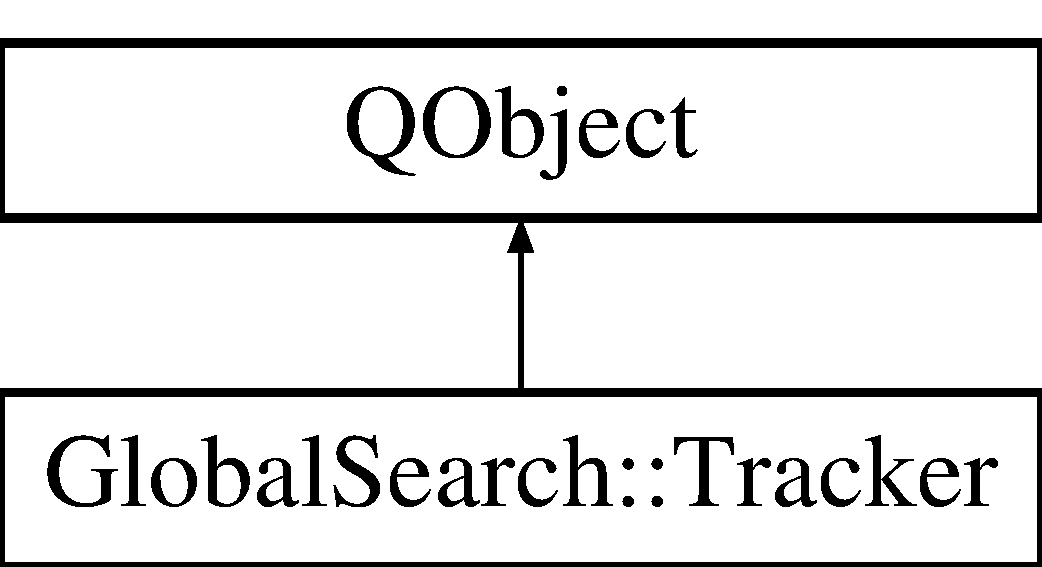
\includegraphics[height=2.000000cm]{classGlobalSearch_1_1Tracker}
\end{center}
\end{figure}
\subsection*{Signals}
\begin{DoxyCompactItemize}
\item 
void \hyperlink{classGlobalSearch_1_1Tracker_ab52b21fb3c4af98fe959bb904f6d029d}{new\+Structure\+Added} (\hyperlink{classGlobalSearch_1_1Structure}{Global\+Search\+::\+Structure} $\ast$s)
\item 
void \hyperlink{classGlobalSearch_1_1Tracker_aa678a5cf9b95b57c51ae19dd6a116613}{structure\+Count\+Changed} (int c)
\end{DoxyCompactItemize}
\subsection*{Public Member Functions}
\begin{DoxyCompactItemize}
\item 
\hyperlink{classGlobalSearch_1_1Tracker_ae61188a8f66c57cc303a823da6130f25}{Tracker} (Q\+Object $\ast$parent=0)
\item 
virtual \hyperlink{classGlobalSearch_1_1Tracker_a231c0a58d7023188e0b9118924fac506}{$\sim$\+Tracker} ()
\item 
void \hyperlink{classGlobalSearch_1_1Tracker_afa0bbd85ec04527c7919a29746e235e4}{lock\+For\+Read} ()
\item 
void \hyperlink{classGlobalSearch_1_1Tracker_aba8064ec469694aa7207b734ac075fad}{lock\+For\+Write} ()
\item 
void \hyperlink{classGlobalSearch_1_1Tracker_a3c30e04b28dd39ddeff887d3bf4e812a}{unlock} ()
\item 
Q\+Read\+Write\+Lock $\ast$ \hyperlink{classGlobalSearch_1_1Tracker_a4aa19e3357f6803957c5646c4bb8f530}{rw\+Lock} ()
\item 
Q\+List$<$ \hyperlink{classGlobalSearch_1_1Structure}{Structure} $\ast$ $>$ $\ast$ \hyperlink{classGlobalSearch_1_1Tracker_a2d8fc282ef5d400a48f5afb931eeba8b}{list} ()
\item 
\hyperlink{classGlobalSearch_1_1Structure}{Structure} $\ast$ \hyperlink{classGlobalSearch_1_1Tracker_ab1457df5dea634a1f9b482cab0c8edb0}{at} (int i)
\item 
bool \hyperlink{classGlobalSearch_1_1Tracker_aebafa2ceea4e665f2660917eb18eb4b5}{append} (Q\+List$<$ \hyperlink{classGlobalSearch_1_1Structure}{Structure} $\ast$ $>$ s)
\item 
bool \hyperlink{classGlobalSearch_1_1Tracker_a1b1705061e58e92e1650e91cb44a07f6}{append} (\hyperlink{classGlobalSearch_1_1Structure}{Structure} $\ast$s)
\item 
bool \hyperlink{classGlobalSearch_1_1Tracker_a7e022f8bd6943c5eb0651f81ce369793}{pop\+First} (\hyperlink{classGlobalSearch_1_1Structure}{Structure} $\ast$\&s)
\item 
bool \hyperlink{classGlobalSearch_1_1Tracker_ad8a31bd3a5185e88157b3a61fdf48a27}{remove} (\hyperlink{classGlobalSearch_1_1Structure}{Structure} $\ast$s)
\item 
bool \hyperlink{classGlobalSearch_1_1Tracker_aa6feecde63a4483355a3672e1dd137dc}{contains} (\hyperlink{classGlobalSearch_1_1Structure}{Structure} $\ast$s)
\item 
int \hyperlink{classGlobalSearch_1_1Tracker_a3670df88ce17cde7984de8cf72ed189b}{size} ()
\item 
void \hyperlink{classGlobalSearch_1_1Tracker_a585a3720623c0df6f793e7b1b8fc586b}{reset} ()
\item 
void \hyperlink{classGlobalSearch_1_1Tracker_a29171b414ff3092c73113565e838bcc1}{delete\+All\+Structures} ()
\end{DoxyCompactItemize}


\subsection{Detailed Description}
The \hyperlink{classGlobalSearch_1_1Tracker}{Tracker} contains a thread-\/safe list of unique Structures. 

\begin{DoxyAuthor}{Author}
David C. Lonie
\end{DoxyAuthor}
In simplest terms, the \hyperlink{classGlobalSearch_1_1Tracker}{Tracker} class is a list of Structures. It provides convenience functions and signals to facilitate access.

The \hyperlink{classGlobalSearch_1_1Tracker}{Tracker} can be used for storage of all Structures generated in a search, or as a F\+I\+F\+O buffer for pending operations by using the \hyperlink{classGlobalSearch_1_1Tracker_aebafa2ceea4e665f2660917eb18eb4b5}{append()} and \hyperlink{classGlobalSearch_1_1Tracker_a7e022f8bd6943c5eb0651f81ce369793}{pop\+First()} functions.

If you wish to not use the convenience functions, it is possible to access the list of Structures through \hyperlink{classGlobalSearch_1_1Tracker_a2d8fc282ef5d400a48f5afb931eeba8b}{list()} and the mutex through \hyperlink{classGlobalSearch_1_1Tracker_a4aa19e3357f6803957c5646c4bb8f530}{rw\+Lock()}, \hyperlink{classGlobalSearch_1_1Tracker_afa0bbd85ec04527c7919a29746e235e4}{lock\+For\+Read()}, \hyperlink{classGlobalSearch_1_1Tracker_aba8064ec469694aa7207b734ac075fad}{lock\+For\+Write()}, and \hyperlink{classGlobalSearch_1_1Tracker_a3c30e04b28dd39ddeff887d3bf4e812a}{unlock()}. 

Definition at line 43 of file tracker.\+h.



\subsection{Constructor \& Destructor Documentation}
\hypertarget{classGlobalSearch_1_1Tracker_ae61188a8f66c57cc303a823da6130f25}{}\index{Global\+Search\+::\+Tracker@{Global\+Search\+::\+Tracker}!Tracker@{Tracker}}
\index{Tracker@{Tracker}!Global\+Search\+::\+Tracker@{Global\+Search\+::\+Tracker}}
\subsubsection[{Tracker}]{\setlength{\rightskip}{0pt plus 5cm}Global\+Search\+::\+Tracker\+::\+Tracker (
\begin{DoxyParamCaption}
\item[{Q\+Object $\ast$}]{parent = {\ttfamily 0}}
\end{DoxyParamCaption}
)}\label{classGlobalSearch_1_1Tracker_ae61188a8f66c57cc303a823da6130f25}
Constructor.


\begin{DoxyParams}{Parameters}
{\em parent} & The object parent. \\
\hline
\end{DoxyParams}


Definition at line 30 of file tracker.\+cpp.

\hypertarget{classGlobalSearch_1_1Tracker_a231c0a58d7023188e0b9118924fac506}{}\index{Global\+Search\+::\+Tracker@{Global\+Search\+::\+Tracker}!````~Tracker@{$\sim$\+Tracker}}
\index{````~Tracker@{$\sim$\+Tracker}!Global\+Search\+::\+Tracker@{Global\+Search\+::\+Tracker}}
\subsubsection[{$\sim$\+Tracker}]{\setlength{\rightskip}{0pt plus 5cm}Global\+Search\+::\+Tracker\+::$\sim$\+Tracker (
\begin{DoxyParamCaption}
{}
\end{DoxyParamCaption}
)\hspace{0.3cm}{\ttfamily [virtual]}}\label{classGlobalSearch_1_1Tracker_a231c0a58d7023188e0b9118924fac506}
Destructor. 

Definition at line 35 of file tracker.\+cpp.



References lock\+For\+Write().



\subsection{Member Function Documentation}
\hypertarget{classGlobalSearch_1_1Tracker_aebafa2ceea4e665f2660917eb18eb4b5}{}\index{Global\+Search\+::\+Tracker@{Global\+Search\+::\+Tracker}!append@{append}}
\index{append@{append}!Global\+Search\+::\+Tracker@{Global\+Search\+::\+Tracker}}
\subsubsection[{append}]{\setlength{\rightskip}{0pt plus 5cm}bool Global\+Search\+::\+Tracker\+::append (
\begin{DoxyParamCaption}
\item[{Q\+List$<$ {\bf Structure} $\ast$ $>$}]{s}
\end{DoxyParamCaption}
)}\label{classGlobalSearch_1_1Tracker_aebafa2ceea4e665f2660917eb18eb4b5}

\begin{DoxyParams}{Parameters}
{\em s} & A list of Structures to append to the \hyperlink{classGlobalSearch_1_1Tracker}{Tracker}\\
\hline
\end{DoxyParams}
\begin{DoxyReturn}{Returns}
true if all Structures were not contained in the list, false if any were already present. 
\end{DoxyReturn}
\begin{DoxyNote}{Note}
If the \hyperlink{classGlobalSearch_1_1Structure}{Structure} is already present, it will not be added again. 

The Structures are compared using pointer values 
\end{DoxyNote}


Definition at line 40 of file tracker.\+cpp.



Referenced by Global\+Search\+::\+Queue\+Manager\+::append\+To\+Job\+Start\+Tracker(), Global\+Search\+::\+Queue\+Manager\+::check\+Population(), and Global\+Search\+::\+Queue\+Manager\+::unlock\+For\+Naming().

\hypertarget{classGlobalSearch_1_1Tracker_a1b1705061e58e92e1650e91cb44a07f6}{}\index{Global\+Search\+::\+Tracker@{Global\+Search\+::\+Tracker}!append@{append}}
\index{append@{append}!Global\+Search\+::\+Tracker@{Global\+Search\+::\+Tracker}}
\subsubsection[{append}]{\setlength{\rightskip}{0pt plus 5cm}bool Global\+Search\+::\+Tracker\+::append (
\begin{DoxyParamCaption}
\item[{{\bf Structure} $\ast$}]{s}
\end{DoxyParamCaption}
)}\label{classGlobalSearch_1_1Tracker_a1b1705061e58e92e1650e91cb44a07f6}

\begin{DoxyParams}{Parameters}
{\em s} & A Structures to append to the \hyperlink{classGlobalSearch_1_1Tracker}{Tracker}\\
\hline
\end{DoxyParams}
\begin{DoxyReturn}{Returns}
true if the \hyperlink{classGlobalSearch_1_1Structure}{Structure} was not contained in the list, false if it were already present.
\end{DoxyReturn}
\begin{DoxyNote}{Note}
If the \hyperlink{classGlobalSearch_1_1Structure}{Structure} is already present, it will not be added again.

The Structures are compared using pointer values 
\end{DoxyNote}


Definition at line 49 of file tracker.\+cpp.



References new\+Structure\+Added(), and structure\+Count\+Changed().

\hypertarget{classGlobalSearch_1_1Tracker_ab1457df5dea634a1f9b482cab0c8edb0}{}\index{Global\+Search\+::\+Tracker@{Global\+Search\+::\+Tracker}!at@{at}}
\index{at@{at}!Global\+Search\+::\+Tracker@{Global\+Search\+::\+Tracker}}
\subsubsection[{at}]{\setlength{\rightskip}{0pt plus 5cm}{\bf Structure}$\ast$ Global\+Search\+::\+Tracker\+::at (
\begin{DoxyParamCaption}
\item[{int}]{i}
\end{DoxyParamCaption}
)\hspace{0.3cm}{\ttfamily [inline]}}\label{classGlobalSearch_1_1Tracker_ab1457df5dea634a1f9b482cab0c8edb0}

\begin{DoxyParams}{Parameters}
{\em i} & The index of the \hyperlink{classGlobalSearch_1_1Structure}{Structure} desired \\
\hline
\end{DoxyParams}
\begin{DoxyReturn}{Returns}
A pointer to the \hyperlink{classGlobalSearch_1_1Structure}{Structure} at index i 
\end{DoxyReturn}


Definition at line 90 of file tracker.\+h.

\hypertarget{classGlobalSearch_1_1Tracker_aa6feecde63a4483355a3672e1dd137dc}{}\index{Global\+Search\+::\+Tracker@{Global\+Search\+::\+Tracker}!contains@{contains}}
\index{contains@{contains}!Global\+Search\+::\+Tracker@{Global\+Search\+::\+Tracker}}
\subsubsection[{contains}]{\setlength{\rightskip}{0pt plus 5cm}bool Global\+Search\+::\+Tracker\+::contains (
\begin{DoxyParamCaption}
\item[{{\bf Structure} $\ast$}]{s}
\end{DoxyParamCaption}
)}\label{classGlobalSearch_1_1Tracker_aa6feecde63a4483355a3672e1dd137dc}
Test if a \hyperlink{classGlobalSearch_1_1Structure}{Structure} is in the \hyperlink{classGlobalSearch_1_1Tracker}{Tracker}\textquotesingle{}s list.


\begin{DoxyParams}{Parameters}
{\em s} & The \hyperlink{classGlobalSearch_1_1Structure}{Structure} to check.\\
\hline
\end{DoxyParams}
\begin{DoxyReturn}{Returns}
True if operation was successful, false if not (i.\+e. \hyperlink{classGlobalSearch_1_1Structure}{Structure} was not in list). 
\end{DoxyReturn}


Definition at line 76 of file tracker.\+cpp.

\hypertarget{classGlobalSearch_1_1Tracker_a29171b414ff3092c73113565e838bcc1}{}\index{Global\+Search\+::\+Tracker@{Global\+Search\+::\+Tracker}!delete\+All\+Structures@{delete\+All\+Structures}}
\index{delete\+All\+Structures@{delete\+All\+Structures}!Global\+Search\+::\+Tracker@{Global\+Search\+::\+Tracker}}
\subsubsection[{delete\+All\+Structures}]{\setlength{\rightskip}{0pt plus 5cm}void Global\+Search\+::\+Tracker\+::delete\+All\+Structures (
\begin{DoxyParamCaption}
{}
\end{DoxyParamCaption}
)}\label{classGlobalSearch_1_1Tracker_a29171b414ff3092c73113565e838bcc1}
Remove and delete from memory all Structures from the list. 

Definition at line 90 of file tracker.\+cpp.



References structure\+Count\+Changed().



Referenced by Global\+Search\+::\+Opt\+Base\+::reset(), and Global\+Search\+::\+Abstract\+Dialog\+::resume\+Session\+\_\+().

\hypertarget{classGlobalSearch_1_1Tracker_a2d8fc282ef5d400a48f5afb931eeba8b}{}\index{Global\+Search\+::\+Tracker@{Global\+Search\+::\+Tracker}!list@{list}}
\index{list@{list}!Global\+Search\+::\+Tracker@{Global\+Search\+::\+Tracker}}
\subsubsection[{list}]{\setlength{\rightskip}{0pt plus 5cm}Q\+List$<${\bf Structure}$\ast$$>$$\ast$ Global\+Search\+::\+Tracker\+::list (
\begin{DoxyParamCaption}
{}
\end{DoxyParamCaption}
)\hspace{0.3cm}{\ttfamily [inline]}}\label{classGlobalSearch_1_1Tracker_a2d8fc282ef5d400a48f5afb931eeba8b}
\begin{DoxyReturn}{Returns}
The \hyperlink{classGlobalSearch_1_1Tracker}{Tracker}\textquotesingle{}s \hyperlink{classGlobalSearch_1_1Structure}{Structure} list 
\end{DoxyReturn}


Definition at line 84 of file tracker.\+h.



Referenced by Global\+Search\+::\+Queue\+Manager\+::check\+Population(), Global\+Search\+::\+Queue\+Manager\+::get\+All\+Duplicate\+Structures(), Global\+Search\+::\+Queue\+Manager\+::get\+All\+Optimized\+Structures(), Global\+Search\+::\+Queue\+Manager\+::get\+All\+Running\+Structures(), Global\+Search\+::\+Queue\+Manager\+::get\+All\+Structures(), and Global\+Search\+::\+Opt\+Base\+::save().

\hypertarget{classGlobalSearch_1_1Tracker_afa0bbd85ec04527c7919a29746e235e4}{}\index{Global\+Search\+::\+Tracker@{Global\+Search\+::\+Tracker}!lock\+For\+Read@{lock\+For\+Read}}
\index{lock\+For\+Read@{lock\+For\+Read}!Global\+Search\+::\+Tracker@{Global\+Search\+::\+Tracker}}
\subsubsection[{lock\+For\+Read}]{\setlength{\rightskip}{0pt plus 5cm}void Global\+Search\+::\+Tracker\+::lock\+For\+Read (
\begin{DoxyParamCaption}
{}
\end{DoxyParamCaption}
)\hspace{0.3cm}{\ttfamily [inline]}}\label{classGlobalSearch_1_1Tracker_afa0bbd85ec04527c7919a29746e235e4}
Sets a read lock on the \hyperlink{classGlobalSearch_1_1Tracker}{Tracker}\textquotesingle{}s mutex. 

Definition at line 64 of file tracker.\+h.



Referenced by Global\+Search\+::\+Queue\+Manager\+::check\+Population(), Global\+Search\+::\+Queue\+Manager\+::get\+All\+Duplicate\+Structures(), Global\+Search\+::\+Queue\+Manager\+::get\+All\+Optimized\+Structures(), Global\+Search\+::\+Queue\+Manager\+::get\+All\+Running\+Structures(), Global\+Search\+::\+Queue\+Manager\+::get\+All\+Structures(), and Global\+Search\+::\+Queue\+Manager\+::lock\+For\+Naming().

\hypertarget{classGlobalSearch_1_1Tracker_aba8064ec469694aa7207b734ac075fad}{}\index{Global\+Search\+::\+Tracker@{Global\+Search\+::\+Tracker}!lock\+For\+Write@{lock\+For\+Write}}
\index{lock\+For\+Write@{lock\+For\+Write}!Global\+Search\+::\+Tracker@{Global\+Search\+::\+Tracker}}
\subsubsection[{lock\+For\+Write}]{\setlength{\rightskip}{0pt plus 5cm}void Global\+Search\+::\+Tracker\+::lock\+For\+Write (
\begin{DoxyParamCaption}
{}
\end{DoxyParamCaption}
)\hspace{0.3cm}{\ttfamily [inline]}}\label{classGlobalSearch_1_1Tracker_aba8064ec469694aa7207b734ac075fad}
Sets a write lock on the \hyperlink{classGlobalSearch_1_1Tracker}{Tracker}\textquotesingle{}s mutex. 

Definition at line 69 of file tracker.\+h.



Referenced by Global\+Search\+::\+Queue\+Manager\+::add\+Manual\+Structure\+Request(), Global\+Search\+::\+Queue\+Manager\+::append\+To\+Job\+Start\+Tracker(), Global\+Search\+::\+Queue\+Manager\+::check\+Population(), Global\+Search\+::\+Opt\+Base\+::reset(), Global\+Search\+::\+Abstract\+Dialog\+::resume\+Session\+\_\+(), Global\+Search\+::\+Queue\+Manager\+::unlock\+For\+Naming(), and $\sim$\+Tracker().

\hypertarget{classGlobalSearch_1_1Tracker_ab52b21fb3c4af98fe959bb904f6d029d}{}\index{Global\+Search\+::\+Tracker@{Global\+Search\+::\+Tracker}!new\+Structure\+Added@{new\+Structure\+Added}}
\index{new\+Structure\+Added@{new\+Structure\+Added}!Global\+Search\+::\+Tracker@{Global\+Search\+::\+Tracker}}
\subsubsection[{new\+Structure\+Added}]{\setlength{\rightskip}{0pt plus 5cm}void Global\+Search\+::\+Tracker\+::new\+Structure\+Added (
\begin{DoxyParamCaption}
\item[{{\bf Global\+Search\+::\+Structure} $\ast$}]{s}
\end{DoxyParamCaption}
)\hspace{0.3cm}{\ttfamily [signal]}}\label{classGlobalSearch_1_1Tracker_ab52b21fb3c4af98fe959bb904f6d029d}
Signal emitted when a new \hyperlink{classGlobalSearch_1_1Structure}{Structure} is added to the \hyperlink{classGlobalSearch_1_1Tracker}{Tracker}. 
\begin{DoxyParams}{Parameters}
{\em s} & A Pointer to the new \hyperlink{classGlobalSearch_1_1Structure}{Structure}. \\
\hline
\end{DoxyParams}


Referenced by append().

\hypertarget{classGlobalSearch_1_1Tracker_a7e022f8bd6943c5eb0651f81ce369793}{}\index{Global\+Search\+::\+Tracker@{Global\+Search\+::\+Tracker}!pop\+First@{pop\+First}}
\index{pop\+First@{pop\+First}!Global\+Search\+::\+Tracker@{Global\+Search\+::\+Tracker}}
\subsubsection[{pop\+First}]{\setlength{\rightskip}{0pt plus 5cm}bool Global\+Search\+::\+Tracker\+::pop\+First (
\begin{DoxyParamCaption}
\item[{{\bf Structure} $\ast$\&}]{s}
\end{DoxyParamCaption}
)}\label{classGlobalSearch_1_1Tracker_a7e022f8bd6943c5eb0651f81ce369793}
Remove and return the first \hyperlink{classGlobalSearch_1_1Structure}{Structure} in the \hyperlink{classGlobalSearch_1_1Tracker}{Tracker}\textquotesingle{}s list. Useful for creating a F\+I\+F\+O buffer.


\begin{DoxyParams}{Parameters}
{\em s} & Becomes the \hyperlink{classGlobalSearch_1_1Structure}{Structure} at index 0 of the \hyperlink{classGlobalSearch_1_1Tracker}{Tracker}\textquotesingle{}s list.\\
\hline
\end{DoxyParams}
\begin{DoxyReturn}{Returns}
True if operation was successful, false if not (i.\+e. the list is empty). 
\end{DoxyReturn}


Definition at line 59 of file tracker.\+cpp.



References structure\+Count\+Changed().



Referenced by Global\+Search\+::\+Queue\+Manager\+::start\+Job().

\hypertarget{classGlobalSearch_1_1Tracker_ad8a31bd3a5185e88157b3a61fdf48a27}{}\index{Global\+Search\+::\+Tracker@{Global\+Search\+::\+Tracker}!remove@{remove}}
\index{remove@{remove}!Global\+Search\+::\+Tracker@{Global\+Search\+::\+Tracker}}
\subsubsection[{remove}]{\setlength{\rightskip}{0pt plus 5cm}bool Global\+Search\+::\+Tracker\+::remove (
\begin{DoxyParamCaption}
\item[{{\bf Structure} $\ast$}]{s}
\end{DoxyParamCaption}
)}\label{classGlobalSearch_1_1Tracker_ad8a31bd3a5185e88157b3a61fdf48a27}
Remove a \hyperlink{classGlobalSearch_1_1Structure}{Structure} in the \hyperlink{classGlobalSearch_1_1Tracker}{Tracker}\textquotesingle{}s list.


\begin{DoxyParams}{Parameters}
{\em s} & The \hyperlink{classGlobalSearch_1_1Structure}{Structure} to remove.\\
\hline
\end{DoxyParams}
\begin{DoxyReturn}{Returns}
True if operation was successful, false if not (i.\+e. \hyperlink{classGlobalSearch_1_1Structure}{Structure} was not in list). 
\end{DoxyReturn}
\begin{DoxyNote}{Note}
This does not delete the \hyperlink{classGlobalSearch_1_1Structure}{Structure} from memory. 
\end{DoxyNote}


Definition at line 68 of file tracker.\+cpp.



References structure\+Count\+Changed().



Referenced by Global\+Search\+::\+Queue\+Manager\+::check\+Population().

\hypertarget{classGlobalSearch_1_1Tracker_a585a3720623c0df6f793e7b1b8fc586b}{}\index{Global\+Search\+::\+Tracker@{Global\+Search\+::\+Tracker}!reset@{reset}}
\index{reset@{reset}!Global\+Search\+::\+Tracker@{Global\+Search\+::\+Tracker}}
\subsubsection[{reset}]{\setlength{\rightskip}{0pt plus 5cm}void Global\+Search\+::\+Tracker\+::reset (
\begin{DoxyParamCaption}
{}
\end{DoxyParamCaption}
)}\label{classGlobalSearch_1_1Tracker_a585a3720623c0df6f793e7b1b8fc586b}
Remove all Structures from the list. \begin{DoxyNote}{Note}
This does not delete the Structures from memory. 
\end{DoxyNote}


Definition at line 85 of file tracker.\+cpp.



References structure\+Count\+Changed().



Referenced by Global\+Search\+::\+Opt\+Base\+::reset().

\hypertarget{classGlobalSearch_1_1Tracker_a4aa19e3357f6803957c5646c4bb8f530}{}\index{Global\+Search\+::\+Tracker@{Global\+Search\+::\+Tracker}!rw\+Lock@{rw\+Lock}}
\index{rw\+Lock@{rw\+Lock}!Global\+Search\+::\+Tracker@{Global\+Search\+::\+Tracker}}
\subsubsection[{rw\+Lock}]{\setlength{\rightskip}{0pt plus 5cm}Q\+Read\+Write\+Lock$\ast$ Global\+Search\+::\+Tracker\+::rw\+Lock (
\begin{DoxyParamCaption}
{}
\end{DoxyParamCaption}
)\hspace{0.3cm}{\ttfamily [inline]}}\label{classGlobalSearch_1_1Tracker_a4aa19e3357f6803957c5646c4bb8f530}
\begin{DoxyReturn}{Returns}
The \hyperlink{classGlobalSearch_1_1Tracker}{Tracker}\textquotesingle{}s read-\/write mutex 
\end{DoxyReturn}


Definition at line 79 of file tracker.\+h.



Referenced by Global\+Search\+::\+Opt\+Base\+::save().

\hypertarget{classGlobalSearch_1_1Tracker_a3670df88ce17cde7984de8cf72ed189b}{}\index{Global\+Search\+::\+Tracker@{Global\+Search\+::\+Tracker}!size@{size}}
\index{size@{size}!Global\+Search\+::\+Tracker@{Global\+Search\+::\+Tracker}}
\subsubsection[{size}]{\setlength{\rightskip}{0pt plus 5cm}int Global\+Search\+::\+Tracker\+::size (
\begin{DoxyParamCaption}
{}
\end{DoxyParamCaption}
)}\label{classGlobalSearch_1_1Tracker_a3670df88ce17cde7984de8cf72ed189b}
\begin{DoxyReturn}{Returns}
The number of Structures in the \hyperlink{classGlobalSearch_1_1Tracker}{Tracker}\textquotesingle{}s list. 
\end{DoxyReturn}


Definition at line 81 of file tracker.\+cpp.



Referenced by Global\+Search\+::\+Queue\+Manager\+::check\+Population().

\hypertarget{classGlobalSearch_1_1Tracker_aa678a5cf9b95b57c51ae19dd6a116613}{}\index{Global\+Search\+::\+Tracker@{Global\+Search\+::\+Tracker}!structure\+Count\+Changed@{structure\+Count\+Changed}}
\index{structure\+Count\+Changed@{structure\+Count\+Changed}!Global\+Search\+::\+Tracker@{Global\+Search\+::\+Tracker}}
\subsubsection[{structure\+Count\+Changed}]{\setlength{\rightskip}{0pt plus 5cm}void Global\+Search\+::\+Tracker\+::structure\+Count\+Changed (
\begin{DoxyParamCaption}
\item[{int}]{c}
\end{DoxyParamCaption}
)\hspace{0.3cm}{\ttfamily [signal]}}\label{classGlobalSearch_1_1Tracker_aa678a5cf9b95b57c51ae19dd6a116613}
Signal emitted when then number of Structures in the \hyperlink{classGlobalSearch_1_1Tracker}{Tracker} changes. 
\begin{DoxyParams}{Parameters}
{\em c} & The number of new \hyperlink{classGlobalSearch_1_1Structure}{Structure} in the \hyperlink{classGlobalSearch_1_1Tracker}{Tracker}. \\
\hline
\end{DoxyParams}


Referenced by append(), delete\+All\+Structures(), pop\+First(), remove(), and reset().

\hypertarget{classGlobalSearch_1_1Tracker_a3c30e04b28dd39ddeff887d3bf4e812a}{}\index{Global\+Search\+::\+Tracker@{Global\+Search\+::\+Tracker}!unlock@{unlock}}
\index{unlock@{unlock}!Global\+Search\+::\+Tracker@{Global\+Search\+::\+Tracker}}
\subsubsection[{unlock}]{\setlength{\rightskip}{0pt plus 5cm}void Global\+Search\+::\+Tracker\+::unlock (
\begin{DoxyParamCaption}
{}
\end{DoxyParamCaption}
)\hspace{0.3cm}{\ttfamily [inline]}}\label{classGlobalSearch_1_1Tracker_a3c30e04b28dd39ddeff887d3bf4e812a}
Unlock the \hyperlink{classGlobalSearch_1_1Tracker}{Tracker}\textquotesingle{}s mutex. 

Definition at line 74 of file tracker.\+h.



Referenced by Global\+Search\+::\+Queue\+Manager\+::add\+Manual\+Structure\+Request(), Global\+Search\+::\+Queue\+Manager\+::append\+To\+Job\+Start\+Tracker(), Global\+Search\+::\+Queue\+Manager\+::check\+Population(), Global\+Search\+::\+Queue\+Manager\+::get\+All\+Duplicate\+Structures(), Global\+Search\+::\+Queue\+Manager\+::get\+All\+Optimized\+Structures(), Global\+Search\+::\+Queue\+Manager\+::get\+All\+Running\+Structures(), Global\+Search\+::\+Queue\+Manager\+::get\+All\+Structures(), Global\+Search\+::\+Opt\+Base\+::reset(), Global\+Search\+::\+Abstract\+Dialog\+::resume\+Session\+\_\+(), and Global\+Search\+::\+Queue\+Manager\+::unlock\+For\+Naming().



The documentation for this class was generated from the following files\+:\begin{DoxyCompactItemize}
\item 
src/globalsearch/tracker.\+h\item 
src/globalsearch/tracker.\+cpp\end{DoxyCompactItemize}

%--- End generated contents ---

% Index
\newpage
\phantomsection
\addcontentsline{toc}{chapter}{Index}
\printindex

\end{document}
